% Options for packages loaded elsewhere
% Options for packages loaded elsewhere
\PassOptionsToPackage{unicode}{hyperref}
\PassOptionsToPackage{hyphens}{url}
\PassOptionsToPackage{dvipsnames,svgnames,x11names}{xcolor}
%
\documentclass[
  a4paper,
]{memoir}
\usepackage{xcolor}
\usepackage{amsmath,amssymb}
\setcounter{secnumdepth}{5}
\usepackage{iftex}
\ifPDFTeX
  \usepackage[T1]{fontenc}
  \usepackage[utf8]{inputenc}
  \usepackage{textcomp} % provide euro and other symbols
\else % if luatex or xetex
  \usepackage{unicode-math} % this also loads fontspec
  \defaultfontfeatures{Scale=MatchLowercase}
  \defaultfontfeatures[\rmfamily]{Ligatures=TeX,Scale=1}
\fi
\usepackage{lmodern}
\ifPDFTeX\else
  % xetex/luatex font selection
  \setmainfont[]{Roboto}
  \setsansfont[]{Clancy}
\fi
% Use upquote if available, for straight quotes in verbatim environments
\IfFileExists{upquote.sty}{\usepackage{upquote}}{}
\IfFileExists{microtype.sty}{% use microtype if available
  \usepackage[]{microtype}
  \UseMicrotypeSet[protrusion]{basicmath} % disable protrusion for tt fonts
}{}
\makeatletter
\@ifundefined{KOMAClassName}{% if non-KOMA class
  \IfFileExists{parskip.sty}{%
    \usepackage{parskip}
  }{% else
    \setlength{\parindent}{0pt}
    \setlength{\parskip}{6pt plus 2pt minus 1pt}}
}{% if KOMA class
  \KOMAoptions{parskip=half}}
\makeatother
% Make \paragraph and \subparagraph free-standing
\makeatletter
\ifx\paragraph\undefined\else
  \let\oldparagraph\paragraph
  \renewcommand{\paragraph}{
    \@ifstar
      \xxxParagraphStar
      \xxxParagraphNoStar
  }
  \newcommand{\xxxParagraphStar}[1]{\oldparagraph*{#1}\mbox{}}
  \newcommand{\xxxParagraphNoStar}[1]{\oldparagraph{#1}\mbox{}}
\fi
\ifx\subparagraph\undefined\else
  \let\oldsubparagraph\subparagraph
  \renewcommand{\subparagraph}{
    \@ifstar
      \xxxSubParagraphStar
      \xxxSubParagraphNoStar
  }
  \newcommand{\xxxSubParagraphStar}[1]{\oldsubparagraph*{#1}\mbox{}}
  \newcommand{\xxxSubParagraphNoStar}[1]{\oldsubparagraph{#1}\mbox{}}
\fi
\makeatother

\usepackage{color}
\usepackage{fancyvrb}
\newcommand{\VerbBar}{|}
\newcommand{\VERB}{\Verb[commandchars=\\\{\}]}
\DefineVerbatimEnvironment{Highlighting}{Verbatim}{commandchars=\\\{\}}
% Add ',fontsize=\small' for more characters per line
\usepackage{framed}
\definecolor{shadecolor}{RGB}{255,255,255}
\newenvironment{Shaded}{\begin{snugshade}}{\end{snugshade}}
\newcommand{\AlertTok}[1]{\textcolor[rgb]{0.00,0.00,0.00}{#1}}
\newcommand{\AnnotationTok}[1]{\textcolor[rgb]{0.00,0.00,0.00}{\textit{#1}}}
\newcommand{\AttributeTok}[1]{\textcolor[rgb]{0.00,0.00,0.00}{#1}}
\newcommand{\BaseNTok}[1]{\textcolor[rgb]{0.00,0.00,0.00}{#1}}
\newcommand{\BuiltInTok}[1]{\textcolor[rgb]{0.00,0.00,0.00}{#1}}
\newcommand{\CharTok}[1]{\textcolor[rgb]{0.00,0.00,0.00}{#1}}
\newcommand{\CommentTok}[1]{\textcolor[rgb]{0.00,0.00,0.00}{\textit{#1}}}
\newcommand{\CommentVarTok}[1]{\textcolor[rgb]{0.00,0.00,0.00}{\textit{#1}}}
\newcommand{\ConstantTok}[1]{\textcolor[rgb]{0.00,0.00,0.00}{#1}}
\newcommand{\ControlFlowTok}[1]{\textcolor[rgb]{0.00,0.00,0.00}{#1}}
\newcommand{\DataTypeTok}[1]{\textcolor[rgb]{0.00,0.00,0.00}{#1}}
\newcommand{\DecValTok}[1]{\textcolor[rgb]{0.00,0.00,0.00}{#1}}
\newcommand{\DocumentationTok}[1]{\textcolor[rgb]{0.00,0.00,0.00}{\textit{#1}}}
\newcommand{\ErrorTok}[1]{\textcolor[rgb]{0.00,0.00,0.00}{#1}}
\newcommand{\ExtensionTok}[1]{\textcolor[rgb]{0.00,0.00,0.00}{#1}}
\newcommand{\FloatTok}[1]{\textcolor[rgb]{0.00,0.00,0.00}{#1}}
\newcommand{\FunctionTok}[1]{\textcolor[rgb]{0.00,0.00,0.00}{#1}}
\newcommand{\ImportTok}[1]{\textcolor[rgb]{0.00,0.00,0.00}{#1}}
\newcommand{\InformationTok}[1]{\textcolor[rgb]{0.00,0.00,0.00}{\textit{#1}}}
\newcommand{\KeywordTok}[1]{\textcolor[rgb]{0.00,0.00,0.00}{#1}}
\newcommand{\NormalTok}[1]{\textcolor[rgb]{0.00,0.00,0.00}{#1}}
\newcommand{\OperatorTok}[1]{\textcolor[rgb]{0.00,0.00,0.00}{#1}}
\newcommand{\OtherTok}[1]{\textcolor[rgb]{0.00,0.00,0.00}{#1}}
\newcommand{\PreprocessorTok}[1]{\textcolor[rgb]{0.00,0.00,0.00}{#1}}
\newcommand{\RegionMarkerTok}[1]{\textcolor[rgb]{0.00,0.00,0.00}{#1}}
\newcommand{\SpecialCharTok}[1]{\textcolor[rgb]{0.00,0.00,0.00}{#1}}
\newcommand{\SpecialStringTok}[1]{\textcolor[rgb]{0.00,0.00,0.00}{#1}}
\newcommand{\StringTok}[1]{\textcolor[rgb]{0.00,0.00,0.00}{#1}}
\newcommand{\VariableTok}[1]{\textcolor[rgb]{0.00,0.00,0.00}{#1}}
\newcommand{\VerbatimStringTok}[1]{\textcolor[rgb]{0.00,0.00,0.00}{#1}}
\newcommand{\WarningTok}[1]{\textcolor[rgb]{0.00,0.00,0.00}{\textit{#1}}}

\usepackage{longtable,booktabs,array}
\newcounter{none} % for unnumbered tables
\usepackage{calc} % for calculating minipage widths
% Correct order of tables after \paragraph or \subparagraph
\usepackage{etoolbox}
\makeatletter
\patchcmd\longtable{\par}{\if@noskipsec\mbox{}\fi\par}{}{}
\makeatother
% Allow footnotes in longtable head/foot
\IfFileExists{footnotehyper.sty}{\usepackage{footnotehyper}}{\usepackage{footnote}}
\makesavenoteenv{longtable}
\usepackage{graphicx}
\makeatletter
\newsavebox\pandoc@box
\newcommand*\pandocbounded[1]{% scales image to fit in text height/width
  \sbox\pandoc@box{#1}%
  \Gscale@div\@tempa{\textheight}{\dimexpr\ht\pandoc@box+\dp\pandoc@box\relax}%
  \Gscale@div\@tempb{\linewidth}{\wd\pandoc@box}%
  \ifdim\@tempb\p@<\@tempa\p@\let\@tempa\@tempb\fi% select the smaller of both
  \ifdim\@tempa\p@<\p@\scalebox{\@tempa}{\usebox\pandoc@box}%
  \else\usebox{\pandoc@box}%
  \fi%
}
% Set default figure placement to htbp
\def\fps@figure{htbp}
\makeatother


% definitions for citeproc citations
\NewDocumentCommand\citeproctext{}{}
\NewDocumentCommand\citeproc{mm}{%
  \begingroup\def\citeproctext{#2}\cite{#1}\endgroup}
\makeatletter
 % allow citations to break across lines
 \let\@cite@ofmt\@firstofone
 % avoid brackets around text for \cite:
 \def\@biblabel#1{}
 \def\@cite#1#2{{#1\if@tempswa , #2\fi}}
\makeatother
\newlength{\cslhangindent}
\setlength{\cslhangindent}{1.5em}
\newlength{\csllabelwidth}
\setlength{\csllabelwidth}{3em}
\newenvironment{CSLReferences}[2] % #1 hanging-indent, #2 entry-spacing
 {\begin{list}{}{%
  \setlength{\itemindent}{0pt}
  \setlength{\leftmargin}{0pt}
  \setlength{\parsep}{0pt}
  % turn on hanging indent if param 1 is 1
  \ifodd #1
   \setlength{\leftmargin}{\cslhangindent}
   \setlength{\itemindent}{-1\cslhangindent}
  \fi
  % set entry spacing
  \setlength{\itemsep}{#2\baselineskip}}}
 {\end{list}}
\usepackage{calc}
\newcommand{\CSLBlock}[1]{\hfill\break\parbox[t]{\linewidth}{\strut\ignorespaces#1\strut}}
\newcommand{\CSLLeftMargin}[1]{\parbox[t]{\csllabelwidth}{\strut#1\strut}}
\newcommand{\CSLRightInline}[1]{\parbox[t]{\linewidth - \csllabelwidth}{\strut#1\strut}}
\newcommand{\CSLIndent}[1]{\hspace{\cslhangindent}#1}



\setlength{\emergencystretch}{3em} % prevent overfull lines

\providecommand{\tightlist}{%
  \setlength{\itemsep}{0pt}\setlength{\parskip}{0pt}}



 


\usepackage{booktabs}
\usepackage{float}

\floatstyle{boxed}
\newfloat{program}{thp}{lop}
\floatname{program}{Output}

\usepackage[section]{placeins}
% See https://tex.stackexchange.com/questions/279/how-do-i-ensure-that-figures-appear-in-the-section-theyre-associated-with

% \nonzeroparskip
% % Used to create spacing between paragraphs
% % See https://tex.stackexchange.com/questions/651036/change-line-spacing-along-the-document-in-memoir-class

\usepackage{pdfpages}

\renewcommand{\chaptername}{Module}
\renewcommand*{\chapnamefont}{\normalfont\HUGE\bfseries\sffamily}
\renewcommand*{\chapnumfont}{\normalfont\HUGE\bfseries\sffamily}
\renewcommand*{\chaptitlefont}{\normalfont\HUGE\bfseries\sffamily}

\setsecheadstyle{\sffamily}% Set \section style
\setsubsecheadstyle{\sffamily}% Set \subsection style
\setsubsubsecheadstyle{\sffamily}% Set \subsubsection style

\setlrmarginsandblock{3.5cm}{2.5cm}{*}
\setulmarginsandblock{2.5cm}{*}{1}
\checkandfixthelayout 

\raggedright
\raggedbottom

\nonzeroparskip
\setlength{\parindent}{0pt}


% https://tex.stackexchange.com/questions/61033/setting-toc-depth-not-working
% https://tex.stackexchange.com/questions/3327/turn-on-subsection-numbering-in-memoir
\setcounter{secnumdepth}{3}
\usepackage{float}
\usepackage{tabularray}
\usepackage[normalem]{ulem}
\usepackage{graphicx}
\usepackage{rotating}
\UseTblrLibrary{siunitx}
\NewTableCommand{\tinytableDefineColor}[3]{\definecolor{#1}{#2}{#3}}
\newcommand{\tinytableTabularrayUnderline}[1]{\underline{#1}}
\newcommand{\tinytableTabularrayStrikeout}[1]{\sout{#1}}
\usepackage{fontspec}
\usepackage{multirow}
\usepackage{multicol}
\usepackage{colortbl}
\usepackage{ulem}
\usepackage{hhline}
\newlength\Oldarrayrulewidth
\newlength\Oldtabcolsep
\usepackage{longtable}
\usepackage{array}
\usepackage{hyperref}
\usepackage{wrapfig}
\makeatletter
\@ifpackageloaded{tcolorbox}{}{\usepackage[skins,breakable]{tcolorbox}}
\@ifpackageloaded{fontawesome5}{}{\usepackage{fontawesome5}}
\definecolor{quarto-callout-color}{HTML}{909090}
\definecolor{quarto-callout-note-color}{HTML}{0758E5}
\definecolor{quarto-callout-important-color}{HTML}{CC1914}
\definecolor{quarto-callout-warning-color}{HTML}{EB9113}
\definecolor{quarto-callout-tip-color}{HTML}{00A047}
\definecolor{quarto-callout-caution-color}{HTML}{FC5300}
\definecolor{quarto-callout-color-frame}{HTML}{acacac}
\definecolor{quarto-callout-note-color-frame}{HTML}{4582ec}
\definecolor{quarto-callout-important-color-frame}{HTML}{d9534f}
\definecolor{quarto-callout-warning-color-frame}{HTML}{f0ad4e}
\definecolor{quarto-callout-tip-color-frame}{HTML}{02b875}
\definecolor{quarto-callout-caution-color-frame}{HTML}{fd7e14}
\makeatother
\makeatletter
\@ifpackageloaded{bookmark}{}{\usepackage{bookmark}}
\makeatother
\makeatletter
\@ifpackageloaded{caption}{}{\usepackage{caption}}
\AtBeginDocument{%
\ifdefined\contentsname
  \renewcommand*\contentsname{Table of contents}
\else
  \newcommand\contentsname{Table of contents}
\fi
\ifdefined\listfigurename
  \renewcommand*\listfigurename{List of Figures}
\else
  \newcommand\listfigurename{List of Figures}
\fi
\ifdefined\listtablename
  \renewcommand*\listtablename{List of Tables}
\else
  \newcommand\listtablename{List of Tables}
\fi
\ifdefined\figurename
  \renewcommand*\figurename{Figure}
\else
  \newcommand\figurename{Figure}
\fi
\ifdefined\tablename
  \renewcommand*\tablename{Table}
\else
  \newcommand\tablename{Table}
\fi
}
\@ifpackageloaded{float}{}{\usepackage{float}}
\floatstyle{ruled}
\@ifundefined{c@chapter}{\newfloat{codelisting}{h}{lop}}{\newfloat{codelisting}{h}{lop}[chapter]}
\floatname{codelisting}{Listing}
\newcommand*\listoflistings{\listof{codelisting}{List of Listings}}
\makeatother
\makeatletter
\makeatother
\makeatletter
\@ifpackageloaded{caption}{}{\usepackage{caption}}
\@ifpackageloaded{subcaption}{}{\usepackage{subcaption}}
\makeatother
\usepackage{bookmark}
\IfFileExists{xurl.sty}{\usepackage{xurl}}{} % add URL line breaks if available
\urlstyle{same}
\hypersetup{
  pdftitle={PHCM9795: Foundations of Biostatistics},
  pdfauthor={Timothy Dobbins},
  colorlinks=true,
  linkcolor={blue},
  filecolor={Maroon},
  citecolor={Blue},
  urlcolor={Blue},
  pdfcreator={LaTeX via pandoc}}


\title{PHCM9795: Foundations of Biostatistics}
\author{Timothy Dobbins}
\date{14 July, 2026}
\begin{document}
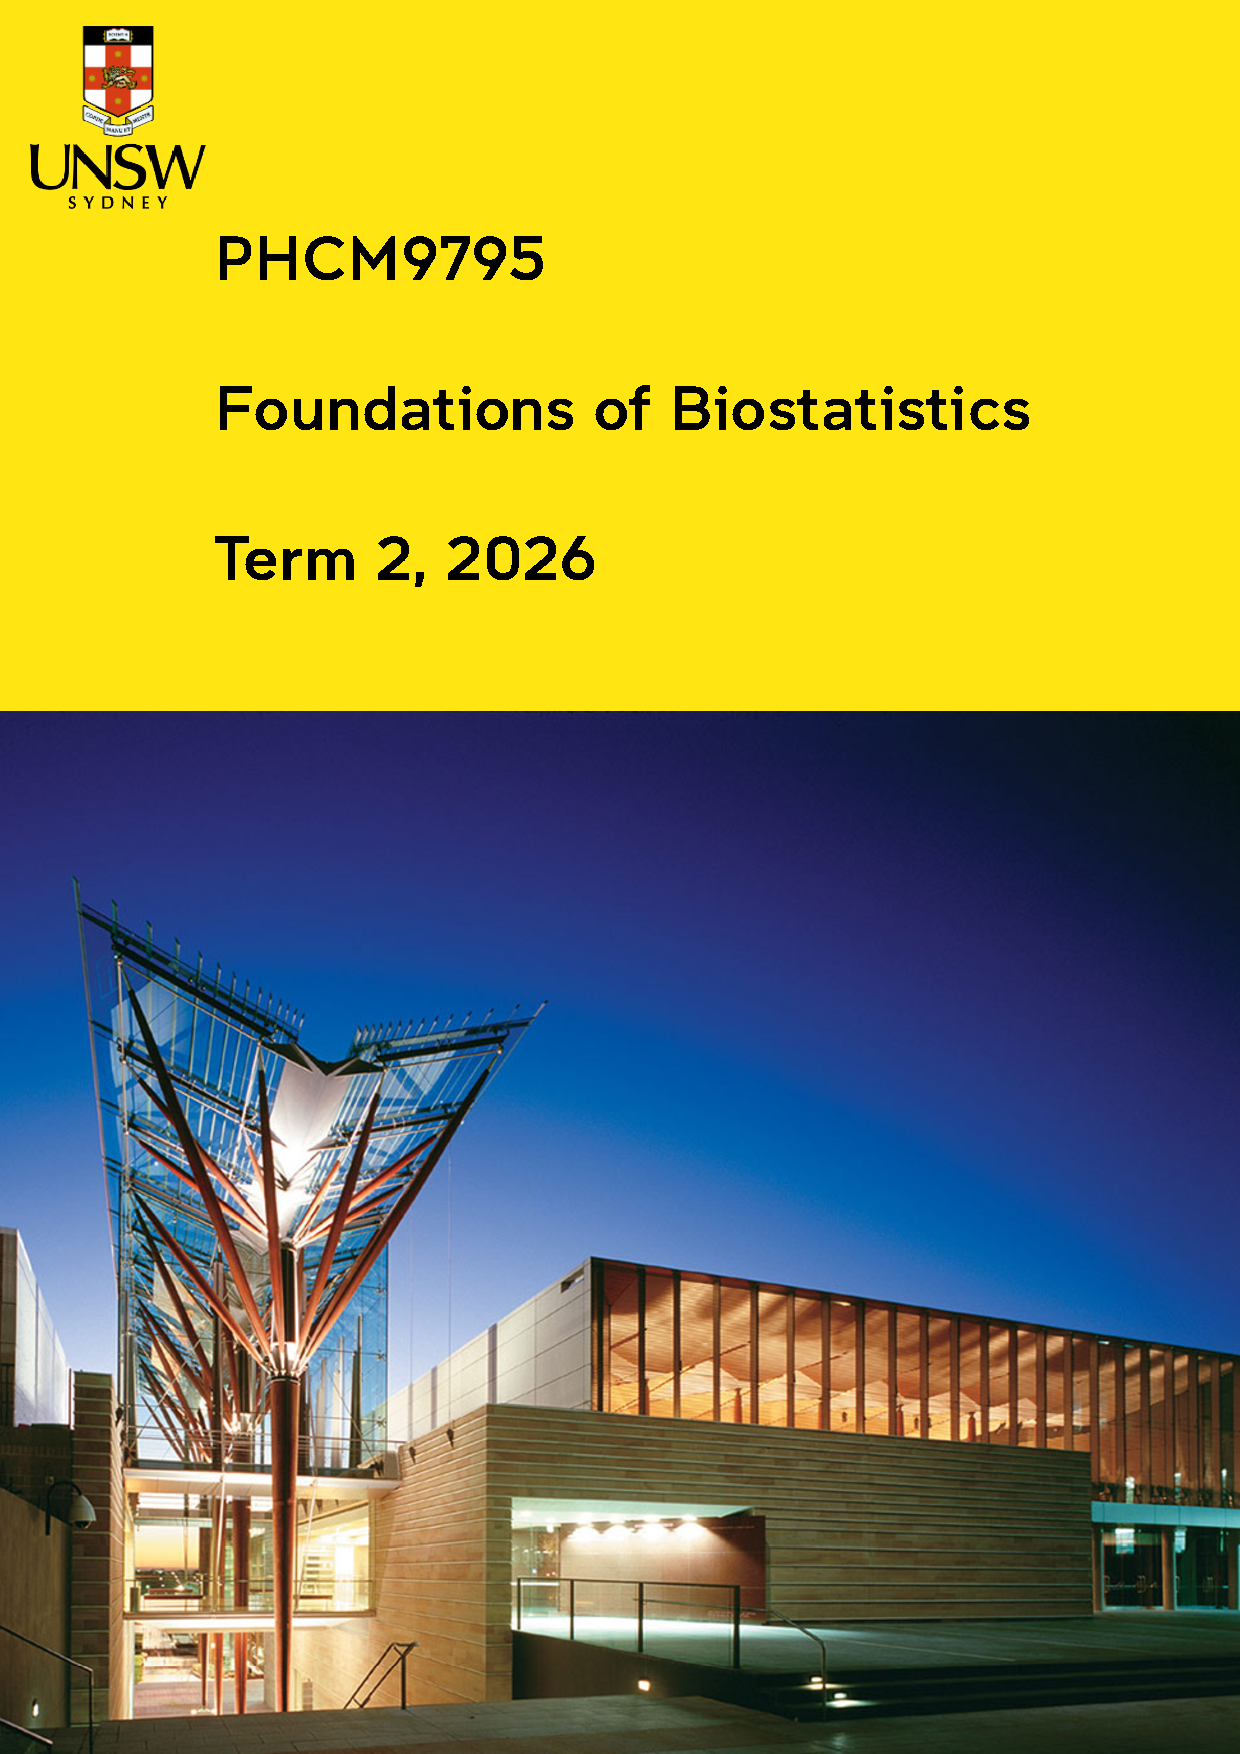
\includepdf[pages=-]{TitlePage2026.pdf}
\clearpage
\frontmatter
\tableofcontents*
\clearpage
\mainmatter

\mainmatter
\bookmarksetup{startatroot}

\chapter*{Course introduction}\label{course-introduction}
\addcontentsline{toc}{chapter}{Course introduction}

\markboth{Course introduction}{Course introduction}

\section*{Welcome}\label{welcome}
\addcontentsline{toc}{section}{Welcome}

\markright{Welcome}

This introductory course in biostatistics aims to provide students with
core biostatistical skills to analyse and present quantitative data from
different study types. These are essential skills required in your
degree and throughout your career.

We hope you enjoy the course and will value your feedback and comment
throughout the course.

\section*{Course information}\label{course-information}
\addcontentsline{toc}{section}{Course information}

\markright{Course information}

Biostatistics is a foundational discipline needed for the analysis and
interpretation of quantitative information and its application to
population health policy and practice.

This course is central to becoming a population health practitioner as
the concepts and techniques developed in the course are fundamental to
your studies and practice in population health. In this course you will
develop an understanding of, and skills in, the core concepts of
biostatistics that are necessary for analysis and interpretation of
population health data and health literature.

In designing this course, we provide a learning sequence that will allow
you to obtain the required graduate capabilities identified for your
program. This course is taught with an emphasis on formulating a
hypothesis and quantifying the evidence in relation to a specific
research question. You will have the opportunity to analyse data from
different study types commonly seen in population health research.

The course will allow those of you who have covered some of this
material in your undergraduate and other professional education to
consolidate your knowledge and skills. Students exposed to biostatistics
for the first time may find the course challenging at times. Based on
student feedback, the key to success in this course is to devote time to
it every week. We recommend that you spend an average of 10-15 hours per
week on the course, including the time spent reading the course notes
and readings, listening to lectures, and working through learning
activities and completing your assessments. Please use the resources
provided to assist you, including online support.

\section*{Course aim}\label{course-aim}
\addcontentsline{toc}{section}{Course aim}

\markright{Course aim}

This course aims to provide students with the core biostatistical skills
to apply appropriate statistical techniques to analyse and present
population health data.

\section*{Learning outcomes}\label{learning-outcomes}
\addcontentsline{toc}{section}{Learning outcomes}

\markright{Learning outcomes}

On successful completion of this course, you will be able to:

\begin{enumerate}
\def\labelenumi{\arabic{enumi}.}
\tightlist
\item
  Summarise and visualise data using statistical software.
\item
  Demonstrate an understanding of statistical inference by interpreting
  p-values and confidence intervals.
\item
  Apply appropriate statistical tests for different types of variables
  given a research question, and interpret computer output of these
  tests appropriately.
\item
  Determine the appropriate sample size when planning a research study.
\item
  Present and interpret statistical findings appropriate for a
  population health audience.
\end{enumerate}

\section*{Suggested reference}\label{suggested-reference}
\addcontentsline{toc}{section}{Suggested reference}

\markright{Suggested reference}

UNSW Sydney, School of Population Health. PHCM9795: Foundations of
Biostatistics Course Notes. UNSW Sydney, 2026.

\section*{Change log}\label{change-log}
\addcontentsline{toc}{section}{Change log}

\markright{Change log}

27 July

\begin{itemize}
\tightlist
\item
  corrected the t-test in Section 9.2 to use a Welch's t-test
\end{itemize}

14 July

\begin{itemize}
\tightlist
\item
  fixed the ordering of the categories in Table 7.5
\end{itemize}

9 June 2026

\begin{itemize}
\tightlist
\item
  updated the address of the Binomial Distribution applet (Module 2) and
  the Normal Distribution applet (Module 3)
\item
  clarified the instructions for Activity 2.5
\end{itemize}

1 June 2026

\begin{itemize}
\tightlist
\item
  Section 1.15 - corrected typo: ``We could use \emph{similar}
  syntax\ldots{}'' Also, the code
  \texttt{sample\$weight\_clean\ =\ ifelse(sample\$weight==700.2,\ NA,\ sample\$weight)}
  should be correctly written as
  \texttt{sample\$weight\_clean\ =\ ifelse(sample\$weight==700.2,\ 70.2,\ sample\$weight)}.
\end{itemize}

\bookmarksetup{startatroot}

\chapter{Introduction to biostatistics and data
fundamentals}\label{introduction-to-biostatistics-and-data-fundamentals}

\section*{Learning objectives}\label{learning-objectives}
\addcontentsline{toc}{section}{Learning objectives}

\markright{Learning objectives}

By the end of this module, you will be able to:

\begin{itemize}
\tightlist
\item
  Understand the difference between descriptive and inferential
  statistics
\item
  Distinguish between different types of variables
\item
  Present and report continuous data numerically and graphically
\item
  Compute summary statistics to describe the centre and spread of data
\end{itemize}

\section*{Optional readings}\label{optional-readings}
\addcontentsline{toc}{section}{Optional readings}

\markright{Optional readings}

Kirkwood and Sterne (2001); Chapters 2, 3 and 4.
\href{http://er1.library.unsw.edu.au/er/cgi-bin/eraccess.cgi?url=https://ebookcentral.proquest.com/lib/unsw/detail.action?docID=624728}{{[}UNSW
Library Link{]}}

Bland (2015); Chapter 4.
\href{http://er1.library.unsw.edu.au/er/cgi-bin/eraccess.cgi?url=https://ebookcentral.proquest.com/lib/unsw/detail.action?docID=5891730}{{[}UNSW
Library Link{]}}

\section{An introduction to
statistics}\label{an-introduction-to-statistics}

The dictionary of statistics (Upton and Cook, 2008) defines statistics
simply as: ``The science of collecting, displaying, and analysing
data.''

Statistics is a branch of mathematics, and there are two main divisions
within the field of statistics: mathematical statistics and applied
statistics. Mathematical statistics deals with development of new
methods of statistical inference and requires detailed knowledge of
abstract mathematics for its implementation. Applied statistics applies
the methods of mathematical statistics to specific subject areas, such
as business, psychology, medicine and sociology.

Biostatistics can be considered as the ``application of statistical
techniques to the medical and health fields''. However, biostatistics
sometimes overlaps with mathematical statistics. For instance, given a
certain biostatistical problem, if the standard methods do not apply
then existing methods must be modified to develop a new method.

\subsection{Scope of Biostatistics}\label{scope-of-biostatistics}

Research is essential in the practice of health care. Biostatistical
knowledge helps health professionals in deciding whether to prescribe a
new drug for the treatment of a disease or to advise a patient to give
up drinking alcohol. To practice evidence-based healthcare, health
professionals must keep abreast of the latest research, which requires
understanding how the studies were designed, how data were collected and
analysed, and how the results were interpreted. In clinical medicine,
biostatistical methods are used to determine the accuracy of a
measurement, the efficacy of a drug in treating a disease, in comparing
different measurement techniques, assessing diagnostic tests,
determining normal values, estimating prognosis and monitoring patients.
Public health professionals are concerned about the administration of
medical services or ensuring that an intervention program reduces
exposure to certain risk factors for disease such as life-style factors
(e.g.~smoking, obesity) or environmental contaminants. Knowledge of
biostatistics helps determine them make decisions by understanding, from
research findings, whether the prevalence of a disease is increasing or
whether there is a causal association between an environmental factor
and a disease.

The value of biostatistics is to transform (sometimes vast amounts of)
data into meaningful information, that can be used to solve problems,
and then be translated into practice (i.e.~to inform public health
policy and decision making). When undertaking research having a
biostatistician as part of a multidisciplinary team from the outset,
together with scientists, clinicians, epidemiologists, healthcare
specialists is vital, to ensure the validity of the research being
undertaken and that information is interpreted appropriately.

\section{What are data?}\label{what-are-data}

According to the Australian Bureau of Statistics, ``data are
measurements or observations that are collected as a source of
information''.\footnote{https://www.abs.gov.au/statistics/understanding-statistics/statistical-terms-and-concepts/data}
Note that technically, the word \emph{data} is a plural noun. This may
sound a little odd, but it means that we say ``data are \ldots{}'' when
discussing a set of measurements.

Other definitions that we use in this course are:

\begin{itemize}
\tightlist
\item
  \textbf{observation}, (or \textbf{record}, or \textbf{unit record}):
  one individual in the population being studied
\item
  \textbf{variable}: a characteristic of an individual being measured.
  For example, height, weight, eye colour, income, country of birth are
  all types of variables.
\item
  \textbf{dataset}: the complete collection of all observations
\end{itemize}

\subsection{Types of variables}\label{types-of-variables}

We can categorise variables into two main types: numeric or categorical.

\textbf{Numerical variables} (also called quantitative variables)
comprise data that must be represented by a number, which can be either
measured or counted.

\textbf{Continuous} variables can take any value within a defined range.

For example, age, height, weight or blood pressure, are continuous
variables because we can make any divisions we want on them, and they
can be measured as small as the instrument allows. As an illustration,
if two people have the same blood pressure measured to the nearest
millimetre of mercury, we may get a difference between them if the blood
pressure is measured to the nearest tenth of millimetre. If they are
still the same (to the nearest tenth of a millimetre), we can measure
them with even finer gradations until we can see a difference.

\textbf{Discrete} variables can only take one of a distinct set of
values (usually whole numbers). For discrete variables, observations are
based on a quantity where both ordering and magnitude are important,
such that numbers represent actual measurable quantities rather than
mere labels.

For example, the number of cancer cases in a specified area emerging
over a certain period, the number of motorbike accidents in Sydney, the
number of times a woman has given birth, the number of beds in a
hospital are all discrete variables. Notice that a natural ordering
exists among the data points, that is, a hospital with 100 beds has more
beds than a hospital with 75 beds. Moreover, a difference between 40 and
50 beds is the same as the difference between 80 and 90 beds.

\textbf{Categorical variables} comprise data that describe a `quality'
or `characteristic'. Categorical variables, sometimes called qualitative
variables, do not have measurable numeric values. Categorical variables
can be nominal or ordinal.

A \textbf{nominal} variable consists of unordered categories. For
example, gender, race, ethnic group, religion, eye colour etc. Both the
order and magnitude of a nominal variable are unimportant.

If a nominal variable takes on one of two distinct categories, such as
black or white then it is called a \textbf{binary} or dichotomous
variable. Other examples would be smoker or non-smoker; exposed to
arsenic or not exposed.

A nominal variable can also have more than two categories, such as blood
group, with categories of: Group A, Group B, Group AB and Group O.

\textbf{Ordinal} variables consist of ordered categories where
differences between categories are important, such as socioeconomic
status (low, medium, high) or student evaluation rating could be
classified according to their level of satisfaction: (highly satisfied,
satisfied and unsatisfied). Here a natural order exists among the
categories.

Note that categorical variables are often stored in data sets using
numbers to represent categories. However, this is for convenience only,
and these variable must not be analysed as if they were numeric
variables.

\section{Descriptive and inferential
statistics}\label{descriptive-and-inferential-statistics}

When analysing a set of data, it is important to consider the aims of
the analysis and whether these are \emph{descriptive} or
\emph{inferential}. Essentially, descriptive statistics summarise data
from a single sample or population, and present a ``snap-shot'' of those
data. Inferential statistics use sample data to make statements about
larger populations.

\subsection{Descriptive statistics}\label{descriptive-statistics}

Descriptive statistics provide a `picture' of the characteristics of a
population, such as the average age, or the proportion of people born in
Australia. Two common examples of descriptive statistics are reports
summarising a nation's birth statistics, and death statistics.

\subsubsection{Births}\label{births}

The Australian Institute of Health and Welfare produces comprehensive
reports on the characteristics of Australia's mothers and babies using
the most recent year of data from the National Perinatal Data
Collection. The National Perinatal Data Collection comprises \emph{all
registered births} in Australia.

The most recent report, published in 2024, summarises Australian births
from 2022. (Australian Institute of Health and Welfare (2024)).

One headline from the report is that ``More First Nations mothers are
accessing antenatal care in the first trimester (up from 51\% in 2013 to
71\% in 2022)''. The report presents further descriptive statistics,
such as the average maternal age (31.2 years) and the proportion of
women giving birth by caesarean (39\%).

\subsubsection{Deaths}\label{deaths}

In another example, consider characteristics of all deaths in Australia
in 2023 (Australian Bureau of Statistics (2024)).

\begin{quote}
``COVID-19 was the ninth leading cause of death in 2023, after ranking
third in 2022.''
\end{quote}

The report presents the leading causes of death in 2023:

\begin{quote}
``The leading cause of death was ischaemic heart disease, accounting for
9.2\% of deaths. The gap between ischaemic heart disease and dementia
(the second leading cause of death) has continued to narrow over time,
with only 237 deaths separating the top two leading causes in 2023.''
\end{quote}

The top five causes of death are also presented as a graph, enabling a
simple comparison of the changes in rates of death between 2014 and
2023.

\begin{figure}

\centering{

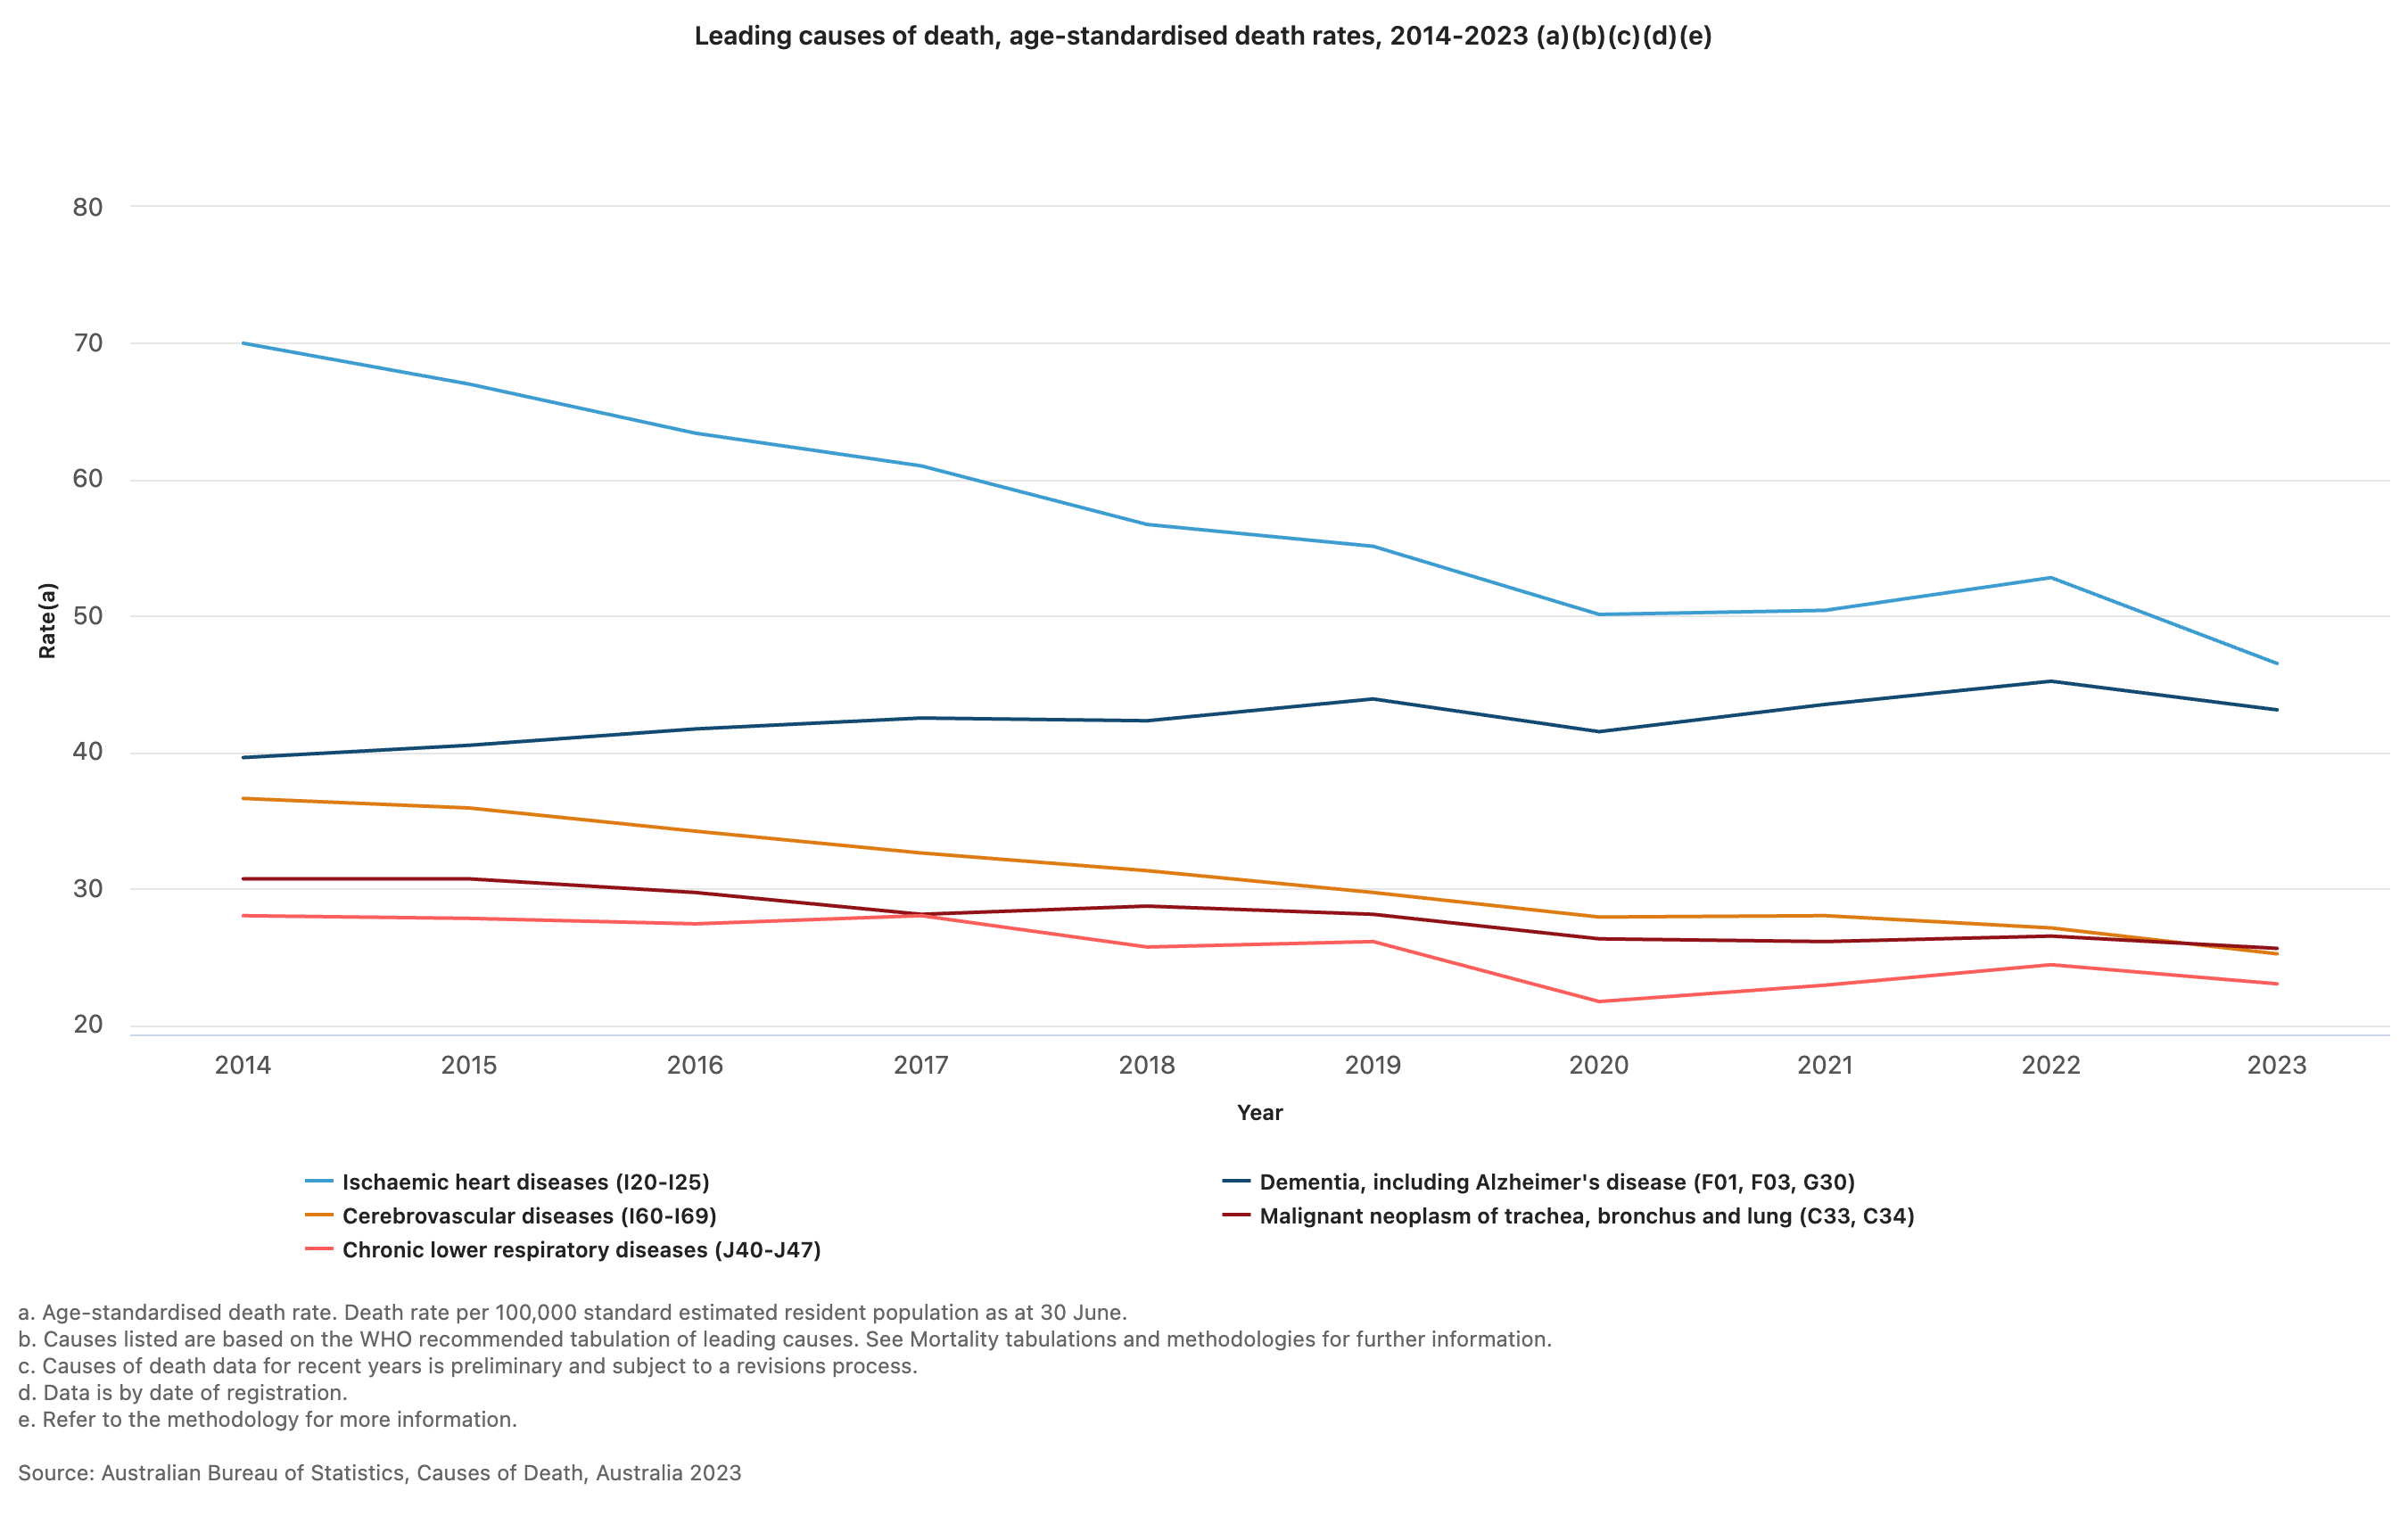
\includegraphics[width=1\linewidth,height=\textheight,keepaspectratio,alt={Line chart showing the top five causes of death in Australia from 2014 to 2023, with age-standardised death rates changing over time.}]{img/mod01/cause-death.png}

}

\caption{\label{fig-1-1}Leading causes of death, age-standardised death
rates, 2014-2023}

\end{figure}%

\subsection{Inferential statistics}\label{inferential-statistics}

Inferential statistics use data collected from a sample to make
conclusions (inferences) about the whole population from which the
sample was drawn. For example, the Australian Institute of Health and
Welfare's \textbf{Australia's health} reports (eg Australian Institute
of Health and Welfare (2025)) use a representative sample to make
estimates of the health of the whole of Australia. We will revisit
\emph{inferential statistics} in later modules.

\section{Summarising continuous data}\label{summarising-continuous-data}

In the first two Modules, we will focus on ways to summarise and present
data. We will see that the choice of presentation will depend on the
type of variable being summarised. In this Module, we will focus on
continuous variables, and will focus on categorical data in Module 2.

\subsection{Summarising a single continuous variable
numerically}\label{summarising-a-single-continuous-variable-numerically}

When summarising continuous data numerically, there are two things we
want to know:

\begin{enumerate}
\def\labelenumi{\arabic{enumi}.}
\tightlist
\item
  What is the average value? And,
\item
  How variable (or spread out) are the data?
\end{enumerate}

We will use a sample of 35 ages (in whole years) to illustrate how to
calculate the average value and measures of variability:

59 41 44 43 31 47 53 59 35 60 54 61 67 52 43 46 39 69 50 64 57 39 54 50
51 31 48 49 70 44 60 51 37 53 34

\subsubsection{Measures of central
tendency}\label{sec-measures-of-central-tendency}

\subsubsection{Mean}\label{mean}

The most commonly used measure of the central tendency of the data is
the mean, calculated as the sum of all the values divided by the number
of values:

\[\bar{x} = \frac{\sum x}{n}\]

From the age example: \(\bar{x}\) = 1745/35 = 49.9. Thus, the mean age
of this sample is 49.9 years.

\subsubsection{Median}\label{median}

Another measure of central tendency is the median. The median is the
middle value of the data, the value at which half of the measurements
lie above it and half of the measurements lie below it.

To estimate the median, the data are ordered from the lowest to highest
values, and the middle value is used. If the middle value is between two
data points (if there are an even number of observations), the median is
an average of the two values.

Using our example, we could rank the ages from smallest to largest, and
locate the middle value (which has been bolded):

31 31 34 35 37 39 39 41 43 43 44 44 46 47 48 49 50 \textbf{50} 51 51 52
53 53 54 54 57 59 59 60 60 61 64 67 69 70

Here, the median age is 50 years.

Note that, in practice, the median is usually calculated by software
automatically, and there is no need to rank our data.

\subsubsection{Describing the spread of the
data}\label{describing-the-spread-of-the-data}

In addition to measuring the centre of the data, we also need an
estimate of the variability, or spread, of the data points.

\subsubsection{Range}\label{range}

The absolute measure of the spread of the data is the range, that is the
difference between the highest and lowest values in the dataset.

Range = highest data value -- lowest data value

Using the age example, Range = 70 - 31 = 39 years.

The range is most usefully reported as the actual lowest and highest
values e.g.~Range: 31 to 70 years.

The range is not always ideal as it only describes the extreme values,
without considering how the bulk of the data is distributed between
them.

\subsubsection{Variance and standard
deviation}\label{variance-and-standard-deviation}

More useful statistics to describe the spread of the data around a mean
value are the variance and standard deviation. These measures of
variability depend on the difference between individual observations and
the mean value (deviations). If all values are equal to the mean there
would be no variability at all, all deviations would be zero; conversely
large deviations indicate greater variability.

One way of combining deviations in a single measure is to first square
the deviations and then average the squares. Squaring is done because we
are equally interested in negative deviations and positive deviations;
if we averaged without squaring, negative and positive deviations would
`cancel out'. This measure is called the variance of the set of
observations. It is `the average squared deviation from the mean'.
Because the variance is in `square' units and not in the units of the
measurement, a second measure is derived by taking the square root of
the variance. This is the standard deviation (SD), and is the most
commonly used measure of variability in practice, as it is a more
intuitive interpretation since it is in the same units as the units of
measurement.

The formula for the variance of a sample (\(s^2\)) is:

\[ s^2 = \frac{\sum(x - \bar{x})^2}{n-1} \]

Note that the deviations are first squared before they are summed to
remove the negative values; once summed they are divided by the sample
size minus 1.

The sample standard deviation is the square root of the of the sample
variance:

\[s = \sqrt{s^2}\] For the age example, we would calculate the sample
variance using statistical software. The sample standard deviation is
estimated as: \(s = 10.47 \text{ years}\).

Characteristics of the standard deviation:

\begin{itemize}
\tightlist
\item
  It is affected by every measurement
\item
  It is in the same units as the measurements
\item
  It can be converted to measures of precision (standard error and 95\%
  confidence intervals) (Module 3)
\end{itemize}

\subsubsection{Interquartile range}\label{interquartile-range}

The inter-quartile range (IQR) describes the range of measurements in
the central 50\% of values lie. This is estimated by calculating the
values that cut the data at the bottom 25\% and top 25\%. The IQR is the
preferred measure of spread when the median has been used to describe
central tendency.

In the age example, the IQR is estimated as 43 to 58 years.

\subsubsection{Population values: mean, variance and standard
deviation}\label{population-values-mean-variance-and-standard-deviation}

The examples above show how the sample mean, range, variance and
standard deviation are calculated from the sample of ages from 35
people. If we had information on the age of the \emph{entire} population
that the sample was drawn from, we could calculate all the summary
statistics described above (for the sample) for the population.

The equation for calculating the population mean is the same as that of
sample mean, though now we denote the population mean as \(\mu\):

\[ \mu = \frac{\sum{x}}{N} \]

Where \(\sum{x}\) represents the sum of the values in the population,
and \(N\) represents the total number of measurements in the population.

To calculate the population variance (\(\sigma^2\)) and standard
deviation(\(\sigma\)), we use a slightly modified version of the
equation for \(s^2\):

\[ \sigma^2 = \frac{\sum(x - \mu)^2}{N} \]

with a population standard deviation of: \(\sigma = \sqrt{\sigma^2}\).

In practice, we rarely have the information for the entire population to
be able to calculate the population mean and standard deviation.
Theoretically, however, these statistics are important for two main
purposes:

\begin{enumerate}
\def\labelenumi{\arabic{enumi}.}
\tightlist
\item
  the characteristics of the normal distribution (the most important
  probability distribution discussed in later modules) are defined by
  the population mean and standard deviation;
\item
  while calculating sample sizes (discussed in later modules) we need
  information about the population standard deviation, which is usually
  obtained from the existing literature.
\end{enumerate}

\subsection{Summarising a single continuous variable
graphically}\label{summarising-a-single-continuous-variable-graphically}

As well as calculating measures of central tendency and spread to
describe the characteristics of the data, a graphical plot can be
helpful to better understand the characteristics and distribution of the
measurements obtained. \emph{Histograms, density plots} and \emph{box
plots} are excellent ways to display continuous data graphically.

\subsubsection{Frequency histograms}\label{frequency-histograms}

A frequency histogram is a plot of the number of observations that fall
within defined ranges of non-overlapping intervals (called bins).
Examples of frequency histograms are given in Figure~\ref{fig-hist-1}.

\begin{figure}

\centering{

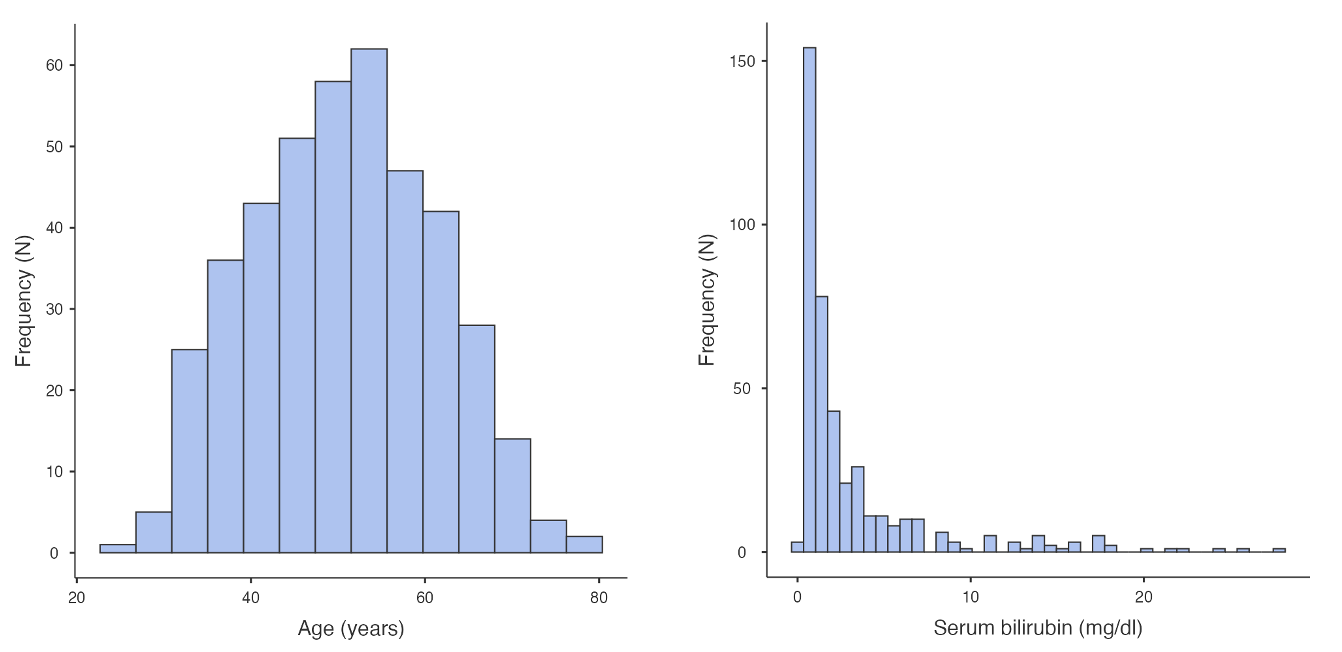
\includegraphics[width=1\linewidth,height=\textheight,keepaspectratio,alt={Two histograms shown side by side, one for age with a roughly symmetric distribution and one for serum bilirubin with a strong right skew.}]{img/mod01/hist-symmetric-skewed.png}

}

\caption{\label{fig-hist-1}Histograms of age and serum bilirubin from
PBC data}

\end{figure}%

Some features of a frequency histogram:

\begin{itemize}
\tightlist
\item
  The area under each rectangle is proportional to the frequency
\item
  The rectangles are drawn without gaps between them (that is, the
  rectangles touch)
\item
  The data are `binned' into discrete intervals (usually of equal width)
\end{itemize}

A slight variation on the frequency histogram is the \textbf{density
histogram}, which plots the density on the y-axis. The density is a
technical term, which is similar to the relative frequency, but is
scaled so that the sum of the area of the bars is equal to 1.

Both the frequency and density histograms are useful for understanding
how the data is distributed across the range of values. Taller bars
indicate regions where the data is more densely concentrated, while
shorter bars represent areas with fewer data points.

\subsubsection{Density plot}\label{density-plot}

A density plot can be thought of as a smoothed version of a density
histogram. Like histograms, density plots show areas where there are a
lot of observations and areas where there are relatively few
observations. Figure~\ref{fig-dens-1} illustrates example density plots
for the same data as plotted in Figure~\ref{fig-hist-1}.

\begin{figure}

\centering{

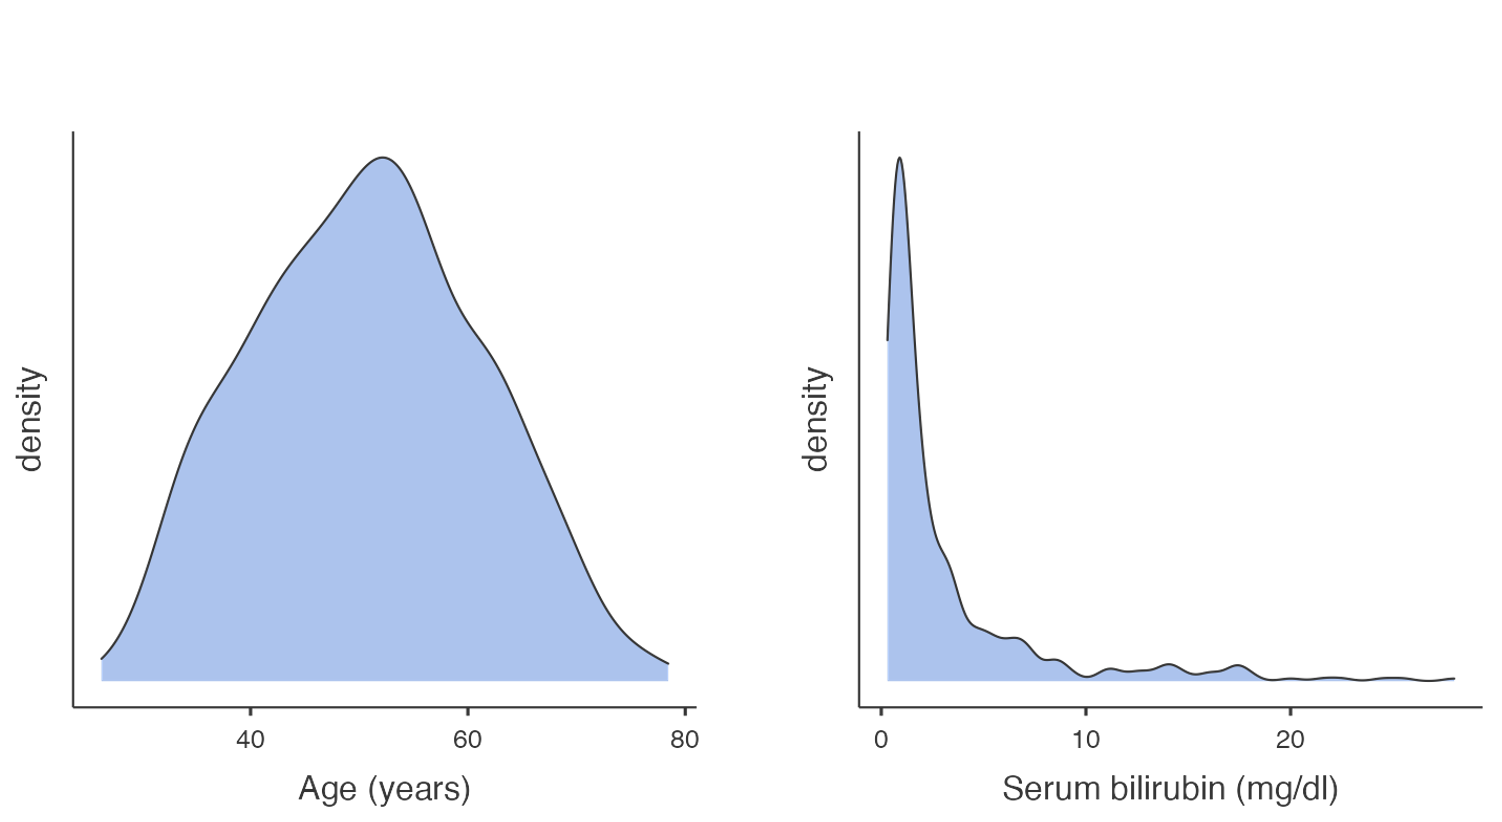
\includegraphics[width=1\linewidth,height=\textheight,keepaspectratio,alt={Two density plots comparing a roughly symmetric age distribution with a highly right-skewed serum bilirubin distribution.}]{img/mod01/dens-symmetric-skewed.png}

}

\caption{\label{fig-dens-1}Density plots of age (left) and serum
bilirubin (right) from a sample of data}

\end{figure}%

Like histograms, density plots allow you to see the overall shape of a
distribution. They are most useful when there are only a small number of
observations being plotted. When plotting small datasets, the shape of a
histogram can depend on how the bins are defined. This is less of an
issue if a density plot is used.

\subsubsection{Boxplots}\label{boxplots}

Another way to inspect the distribution of data is by using a box plot.
In a box plot:

\begin{itemize}
\tightlist
\item
  the line across the box shows the median value
\item
  the limits of the box show the 25-75\% range (i.e.~the inter-quartile
  range (IQR) where the middle 50\% of the data lie)
\item
  the bars (or whiskers) indicate the most extreme values (highest and
  lowest) that fall within 1.5 times the interquartile range from each
  end of the box

  \begin{itemize}
  \tightlist
  \item
    the upper whisker is the highest value falling within 75th
    percentile plus 1.5 × IQR
  \item
    the lower whisker is the lowest value falling within 25th percentile
    minus 1.5 × IQR
  \end{itemize}
\item
  any values in the dataset lying outside the whiskers are plotted
  individually, often labelled by the row number of the observation.
\end{itemize}

Figure~\ref{fig-box-1} presents two example boxplots for age and serum
bilirubin.

\begin{figure}

\centering{

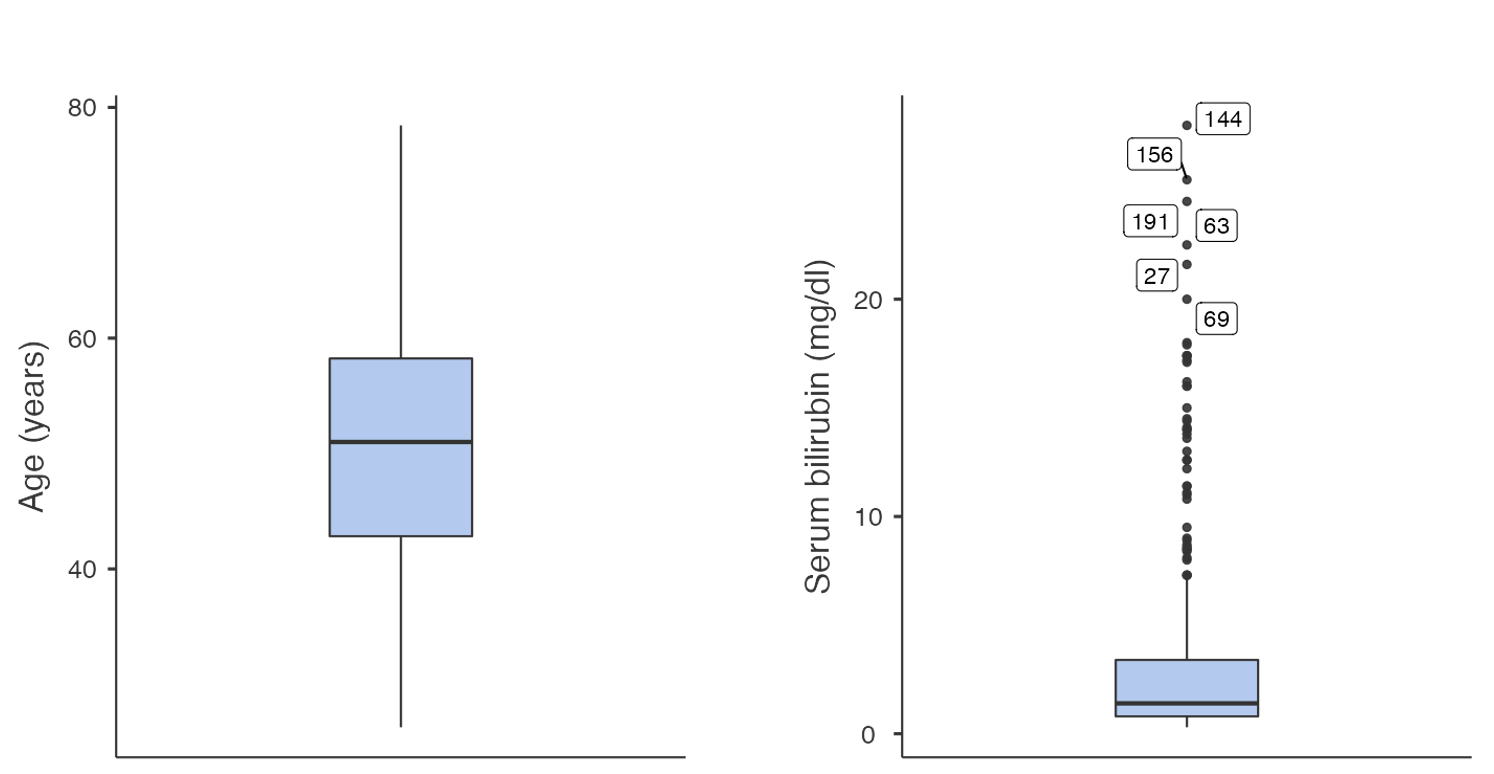
\includegraphics[width=1\linewidth,height=\textheight,keepaspectratio,alt={Two boxplots comparing age and serum bilirubin, with serum bilirubin showing a longer upper tail and more extreme values.}]{img/mod01/boxp-symmetric-skewed.png}

}

\caption{\label{fig-box-1}Box plot of age and serum bilirubin from PBC
study data}

\end{figure}%

\subsection{The shape of a
distribution}\label{the-shape-of-a-distribution}

Histograms and density plots allow us to consider the shape of a
distribution, and in particular, whether a distribution is
\emph{symmetric} or \emph{skewed}.

In a histogram, if the rectangles fall in a roughly symmetric shape
around a single midpoint, we say that the distribution is symmetric.
Similarly, if a density plot looks roughly symmetric around a single
point, the distribution is symmetric.

If the histogram or density plot has a longer tail to the right, then
the data are said to be positively skewed (or skewed to the right); if
the histogram or density plot has an extended tail to the left, then the
data are negatively skewed (or skewed to the left).

\begin{quote}
The skewness of a distribution is defined by the location of the longer
tail in a histogram or density plot, not the location of the peak of the
data.
\end{quote}

From Figure~\ref{fig-hist-1} and Figure~\ref{fig-dens-1}, we can see
that the distribution for age is roughly symmetric, while the
distribution for serum bilirubin is highly positively skewed (or skewed
to the right).

While it is technically possible to determine the shape of a
distribution using a boxplot, a histogram or density plot gives a more
complete illustration of a distribution and would be the preferred
method of assessing shape.

\subsection{Which measure of central tendency to
use}\label{which-measure-of-central-tendency-to-use}

We introduced the mean and median in
Section~\ref{sec-measures-of-central-tendency} as measures of central
tendency. We need to assess the shape of a distribution to answer which
is the more appropriate measure to use.

If a distribution is symmetric, the mean and median will be
approximately equal. However, the mean is the preferred measure of
central tendency as it makes use of every data point, and has more
useful mathematical properties.

The mean is not a good measure of central tendency for skewed
distributions, as the calculation will be influenced by the observations
in the tail of the distribution. The median is the preferred statistic
for describing central tendency in a skewed distribution.

If the data exhibits a symmetric distribution, we use the standard
deviation as the measure of spread. Otherwise, the interquartile range
is preferred.

\section{Exploratory data analysis for continuous
data}\label{sec-eda-cts}

Before conducting any formal analysis, it is good practice to undertake
exploratory data analysis. This analysis step gives you a high-level
overview of your data: what do your data look like, what are the main
features, what shape is the distribution, and are there any unusual
values.

Exploring continuous data is best done by examining plots: specifically
density plots and boxplots. Density plots are useful in determining the
shape of a distribution, to help you decide what summary measures to
use, and what type of analysis to conduct. Boxplots can be useful in
identifying any unusual points - often called outliers.Outliers can be
problematic and the decision to include them or omit them from further
analyses can be difficult.

After detecting any outliers or extreme values, \textbf{do not
automatically exclude them from the analysis}. First, it is important to
check the original data collection form or questionnaire to rule out the
possibility of a data entry error. If the outlier is not a data entry
error, it is then important to decide whether the observation is
biologically possible. This step will usually need to be answered by a
topic expert. If the outlier is biologically possible, it must be
included in the analysis. Only if the outlier is biologically impossible
should it be set to missing.

\newpage{}

\bookmarksetup{startatroot}

\chapter*{An introduction to jamovi}\label{an-introduction-to-jamovi}
\addcontentsline{toc}{chapter}{An introduction to jamovi}

\markboth{An introduction to jamovi}{An introduction to jamovi}

\section{An introduction to jamovi}\label{an-introduction-to-jamovi-1}

\section*{Learning outcomes}\label{learning-outcomes-1}
\addcontentsline{toc}{section}{Learning outcomes}

\markright{Learning outcomes}

By the end of these notes, you will be able to:

\begin{itemize}
\tightlist
\item
  navigate the jamovi interface
\item
  input and import data into jamovi
\item
  use jamovi menus to summarise data
\item
  perform basic data transformations
\item
  assign variable and value labels
\item
  understand the difference between saving data and saving jamovi output
\item
  copy jamovi output to a standard word processing package
\end{itemize}

\section{Introduction}\label{introduction}

From the \href{https://www.jamovi.org/}{jamovi website}:

\begin{quote}
jamovi is a new ``3rd generation'' statistical spreadsheet. Designed
from the ground up to be easy to use, jamovi is a compelling alternative
to costly statistical products such as SPSS and SAS.
\end{quote}

\begin{quote}
jamovi is built on top of the R statistical language, giving you access
to the best the statistics community has to offer. Would you like the R
code for your analyses? jamovi can provide that too.
\end{quote}

\begin{quote}
jamovi will always be free and open - that's one of our core values -
because jamovi is made by the scientific community, for the scientific
community.
\end{quote}

The notes provided in this course will cover the basics of using jamovi:
there is much more to jamovi than we will cover in this course.

\section{Part 1: An introduction to
jamovi}\label{part-1-an-introduction-to-jamovi}

In this very brief section, we will introduce jamovi by calculating the
average of six ages. Open the jamovi package in the usual way (note that
while jamovi is available for Windows, MacOS and linux, most of the
screenshots in these notes will be based on the macOS version.)

\section{Installing jamovi}\label{installing-jamovi}

jamovi can be downloaded for no cost at
\url{https://www.jamovi.org/download.html} for Windows, macOS and linux.
I recommend downloading the ``current'' release (not the ``solid''
release). At the time of writing, Version 2.7.24 is the appropriate
version to use. Download and install jamovi in the usual way.

\section{A simple jamovi analysis}\label{a-simple-jamovi-analysis}

When you first open jamovi, it will look something like the following.

\pandocbounded{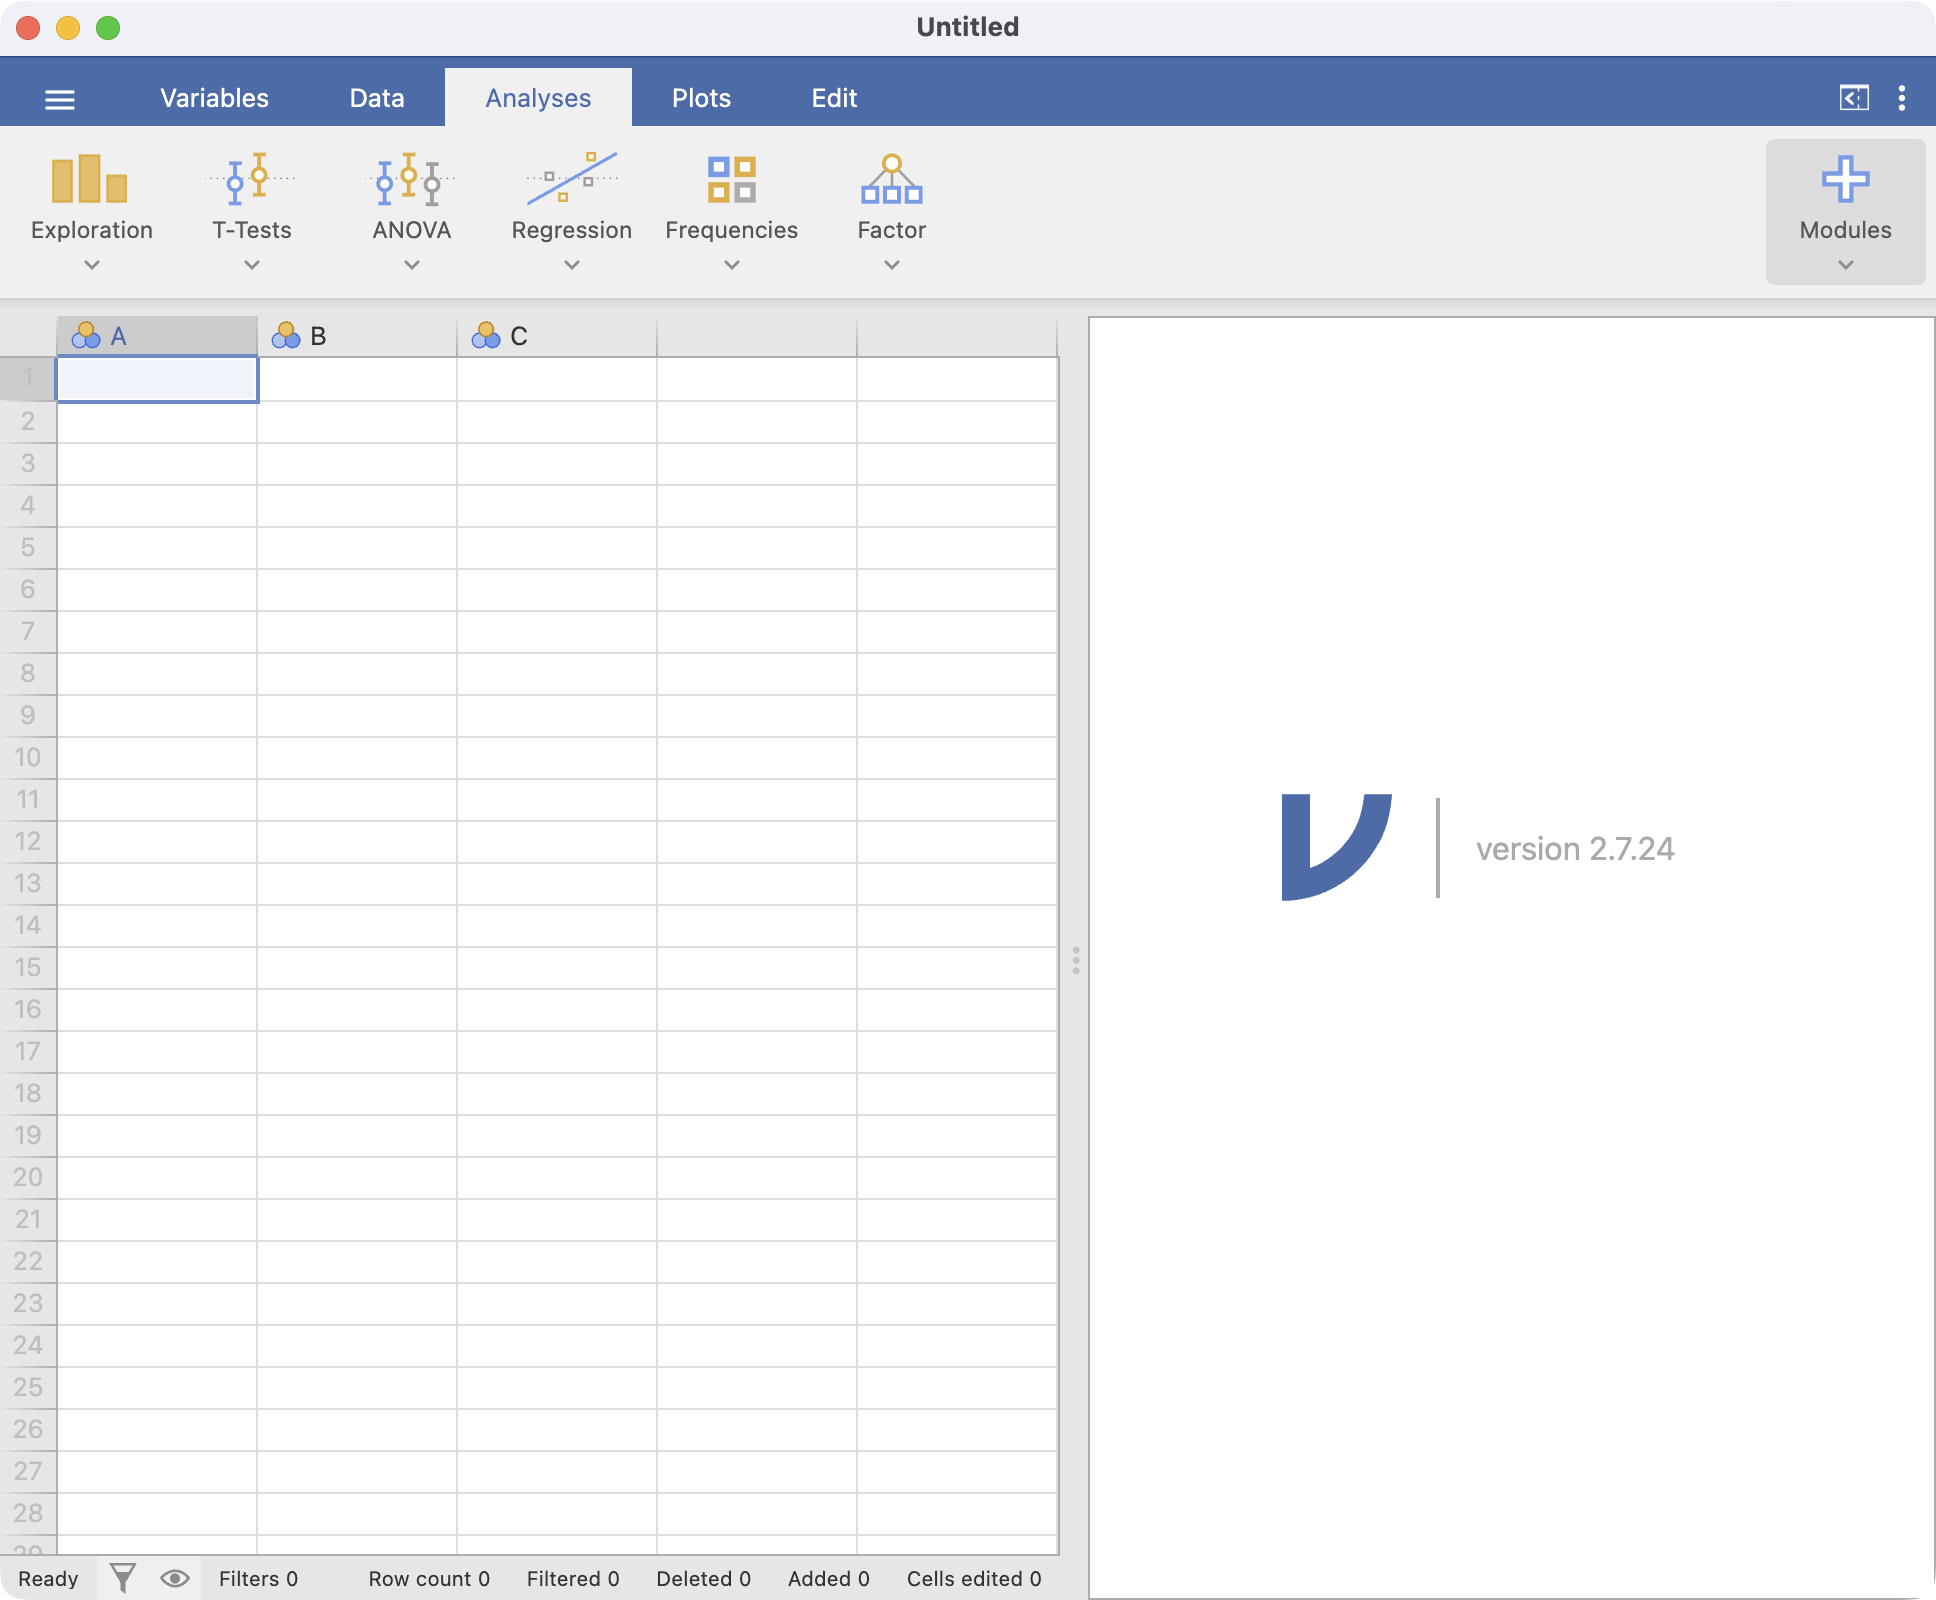
\includegraphics[keepaspectratio]{img/mod01/jamovi/simple-01.png}}
On the left-hand side of the window is the spreadsheet view, and the
right is where results of statistical analyses will appear. The
\textbf{spreadsheet} is where data can be entered or changed.

\begin{tcolorbox}[enhanced jigsaw, arc=.35mm, bottomrule=.15mm, bottomtitle=1mm, breakable, colback=white, colbacktitle=quarto-callout-note-color!10!white, colframe=quarto-callout-note-color-frame, coltitle=black, left=2mm, leftrule=.75mm, opacityback=0, opacitybacktitle=0.6, rightrule=.15mm, title={TASK}, titlerule=0mm, toprule=.15mm, toptitle=1mm]

Enter the following six ages into jamovi, starting at the top-left cell,
by typing each number and then hitting Enter:

\texttt{20\ 25\ 23\ 29\ 21\ 27}

If you make a mistake, simply click the incorrect cell, and enter the
correct value.

\end{tcolorbox}

Your screen should look like this:

\pandocbounded{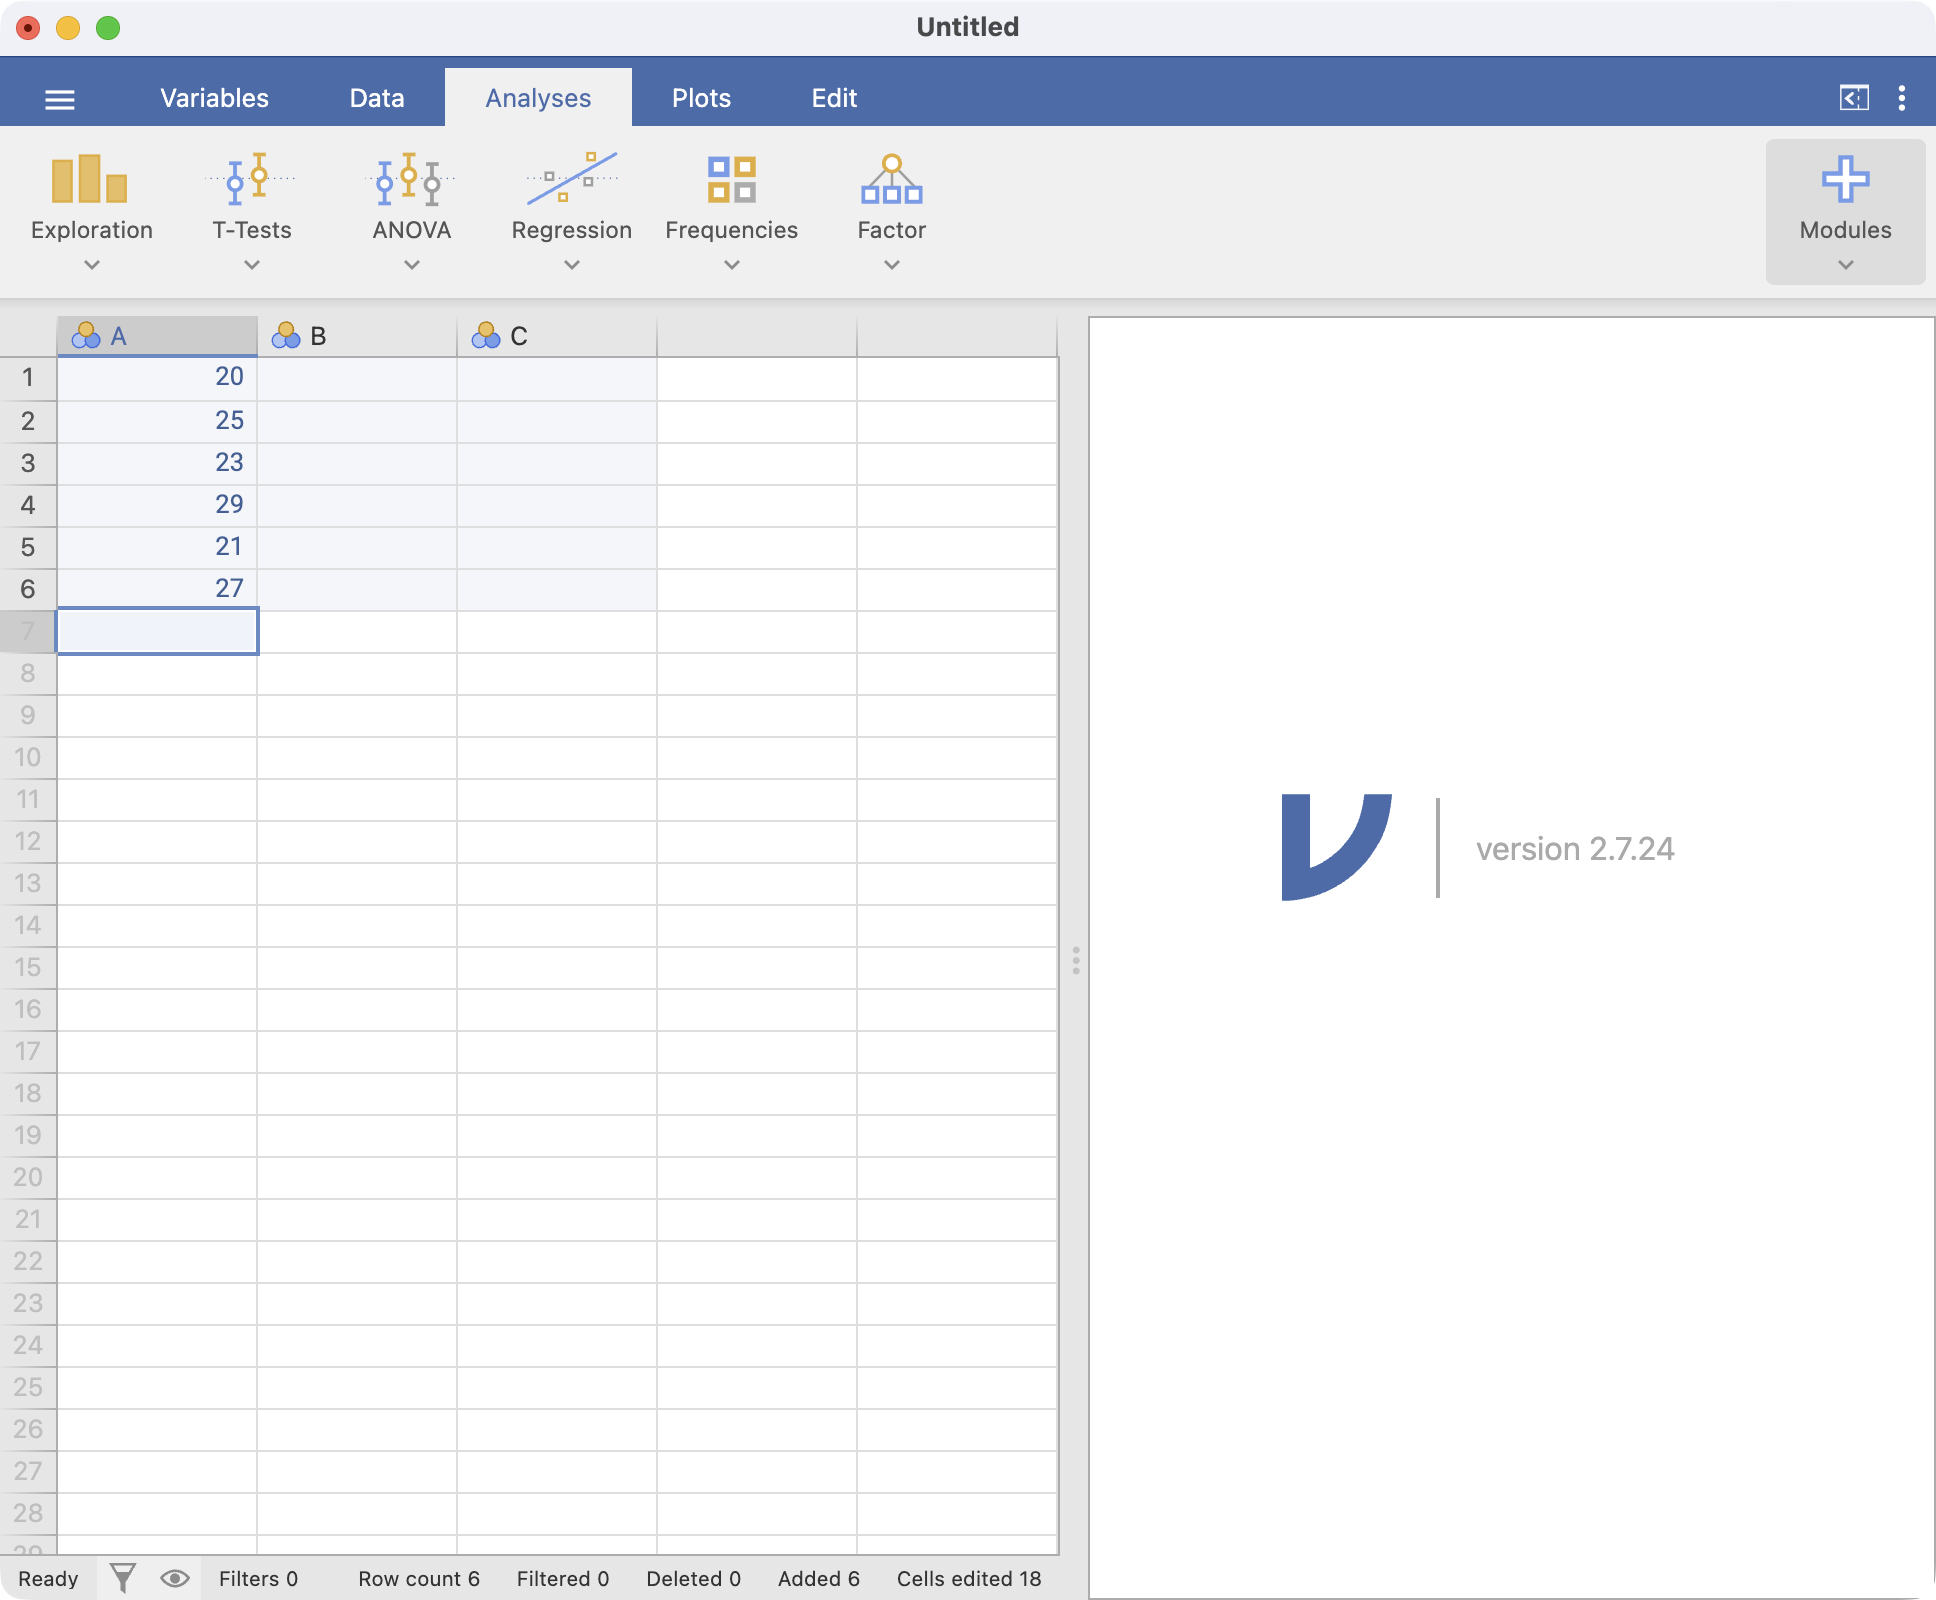
\includegraphics[keepaspectratio]{img/mod01/jamovi/simple-02.png}}

There are two things to note here:

\begin{enumerate}
\def\labelenumi{\arabic{enumi}.}
\tightlist
\item
  Data in jamovi are entered down a column: columns represent variables,
  and rows represent observations. So our six observations of age are
  entered in one column.
\item
  jamovi has given the name of \texttt{A} to our column of ages.
\end{enumerate}

Let's rename our variable from \texttt{A} to \texttt{Age\ (years)}.
There are a number of ways of doing this: here we will click the
\textbf{Data} tab (at the top of the window) which allows us to change
aspects of our dataset, and then click \textbf{Setup}. By default, the
first column is selected - you can choose any column simply by clicking
it.

\pandocbounded{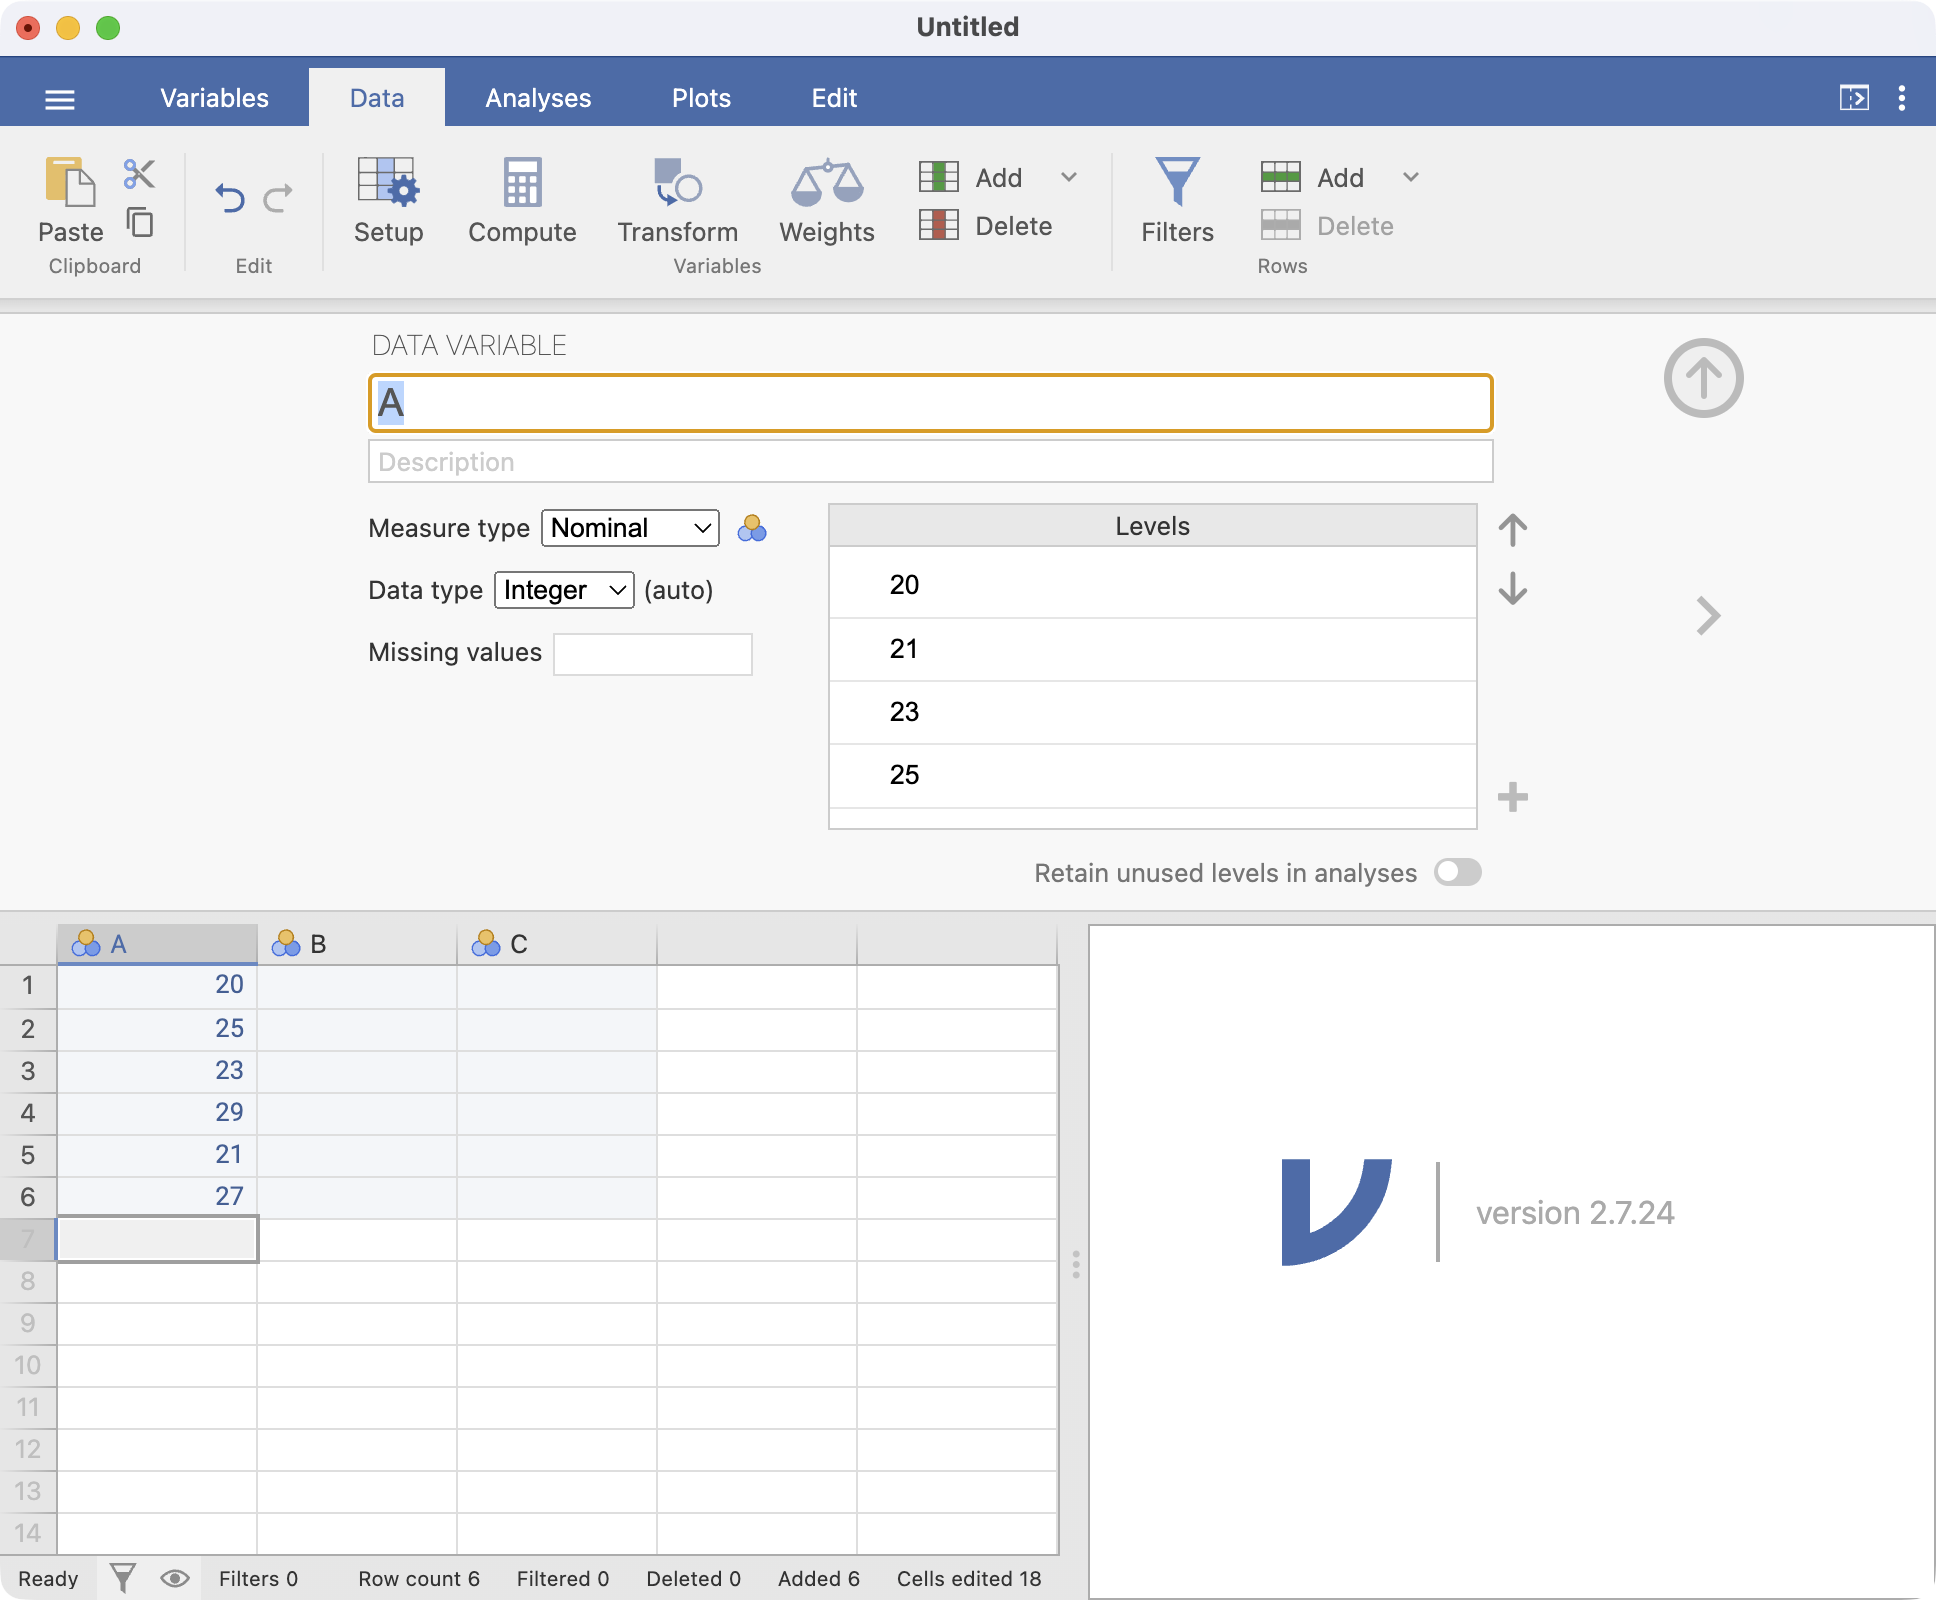
\includegraphics[keepaspectratio]{img/mod01/jamovi/variables-01.png}}

In this window, you can change many variable properties, such as
variable names and variable types. To change the variable name, click
the name of the variable, currently \texttt{A}, at the top of the
window. Replace \texttt{A} with \texttt{Age\ (years)}:

\pandocbounded{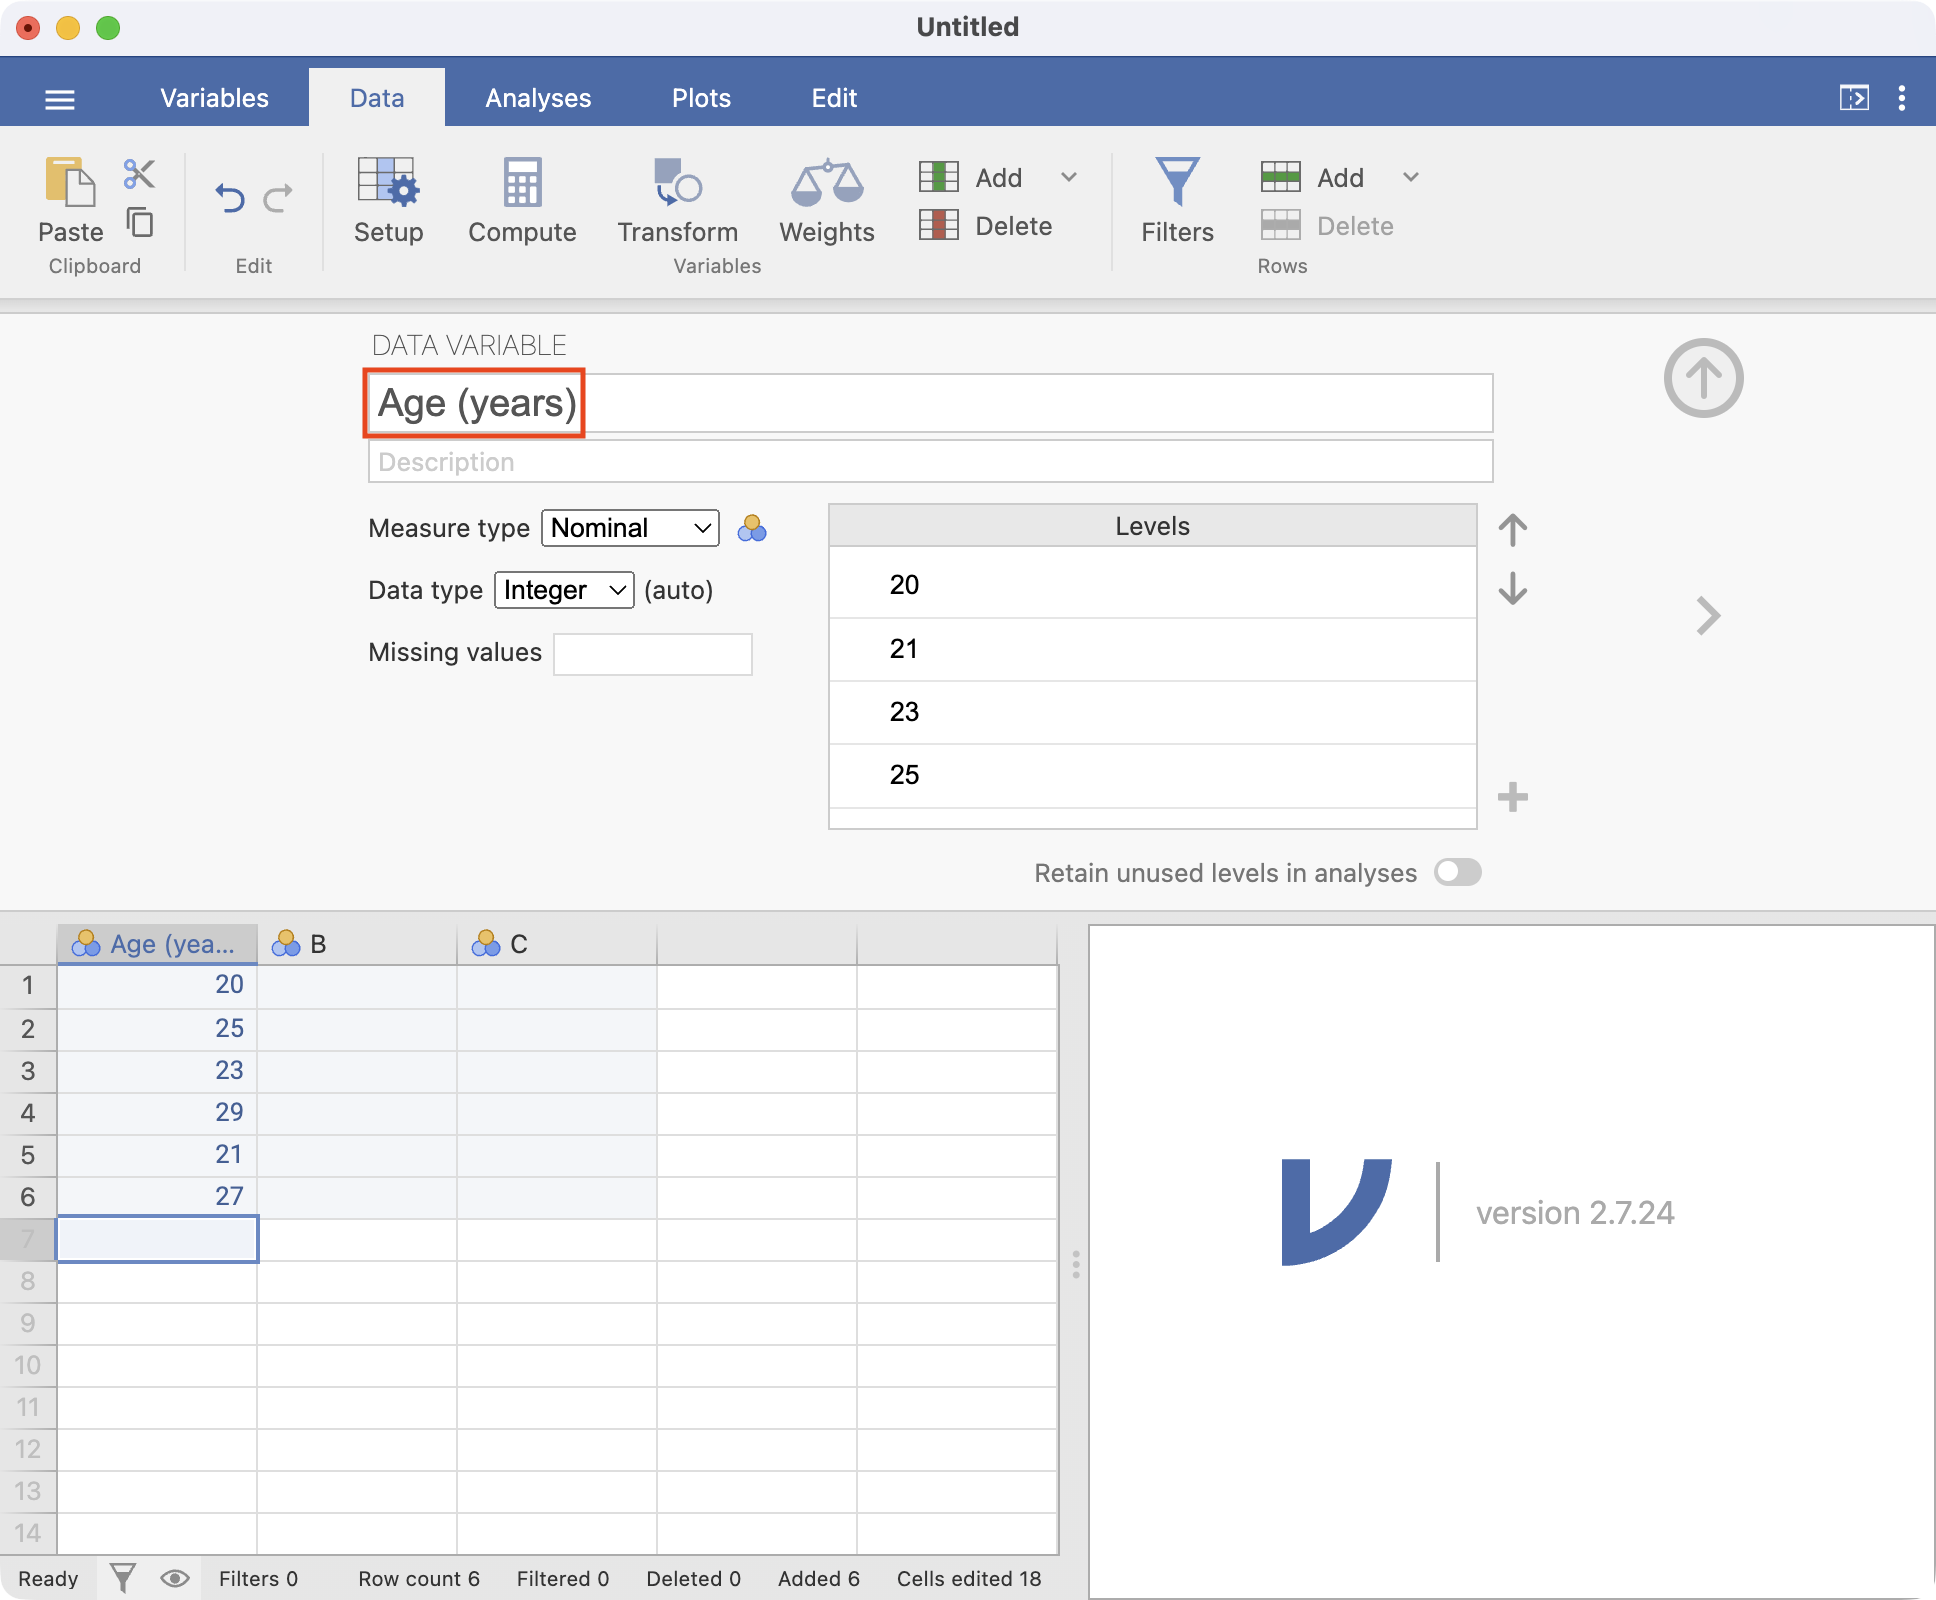
\includegraphics[keepaspectratio]{img/mod01/jamovi/variables-02.png}}

Note that jamovi has assumed these data are \emph{Nominal} data; this
can be changed to \emph{Continuous} by choosing the appropriate item in
the \textbf{Measure type} drop-down menu:

\pandocbounded{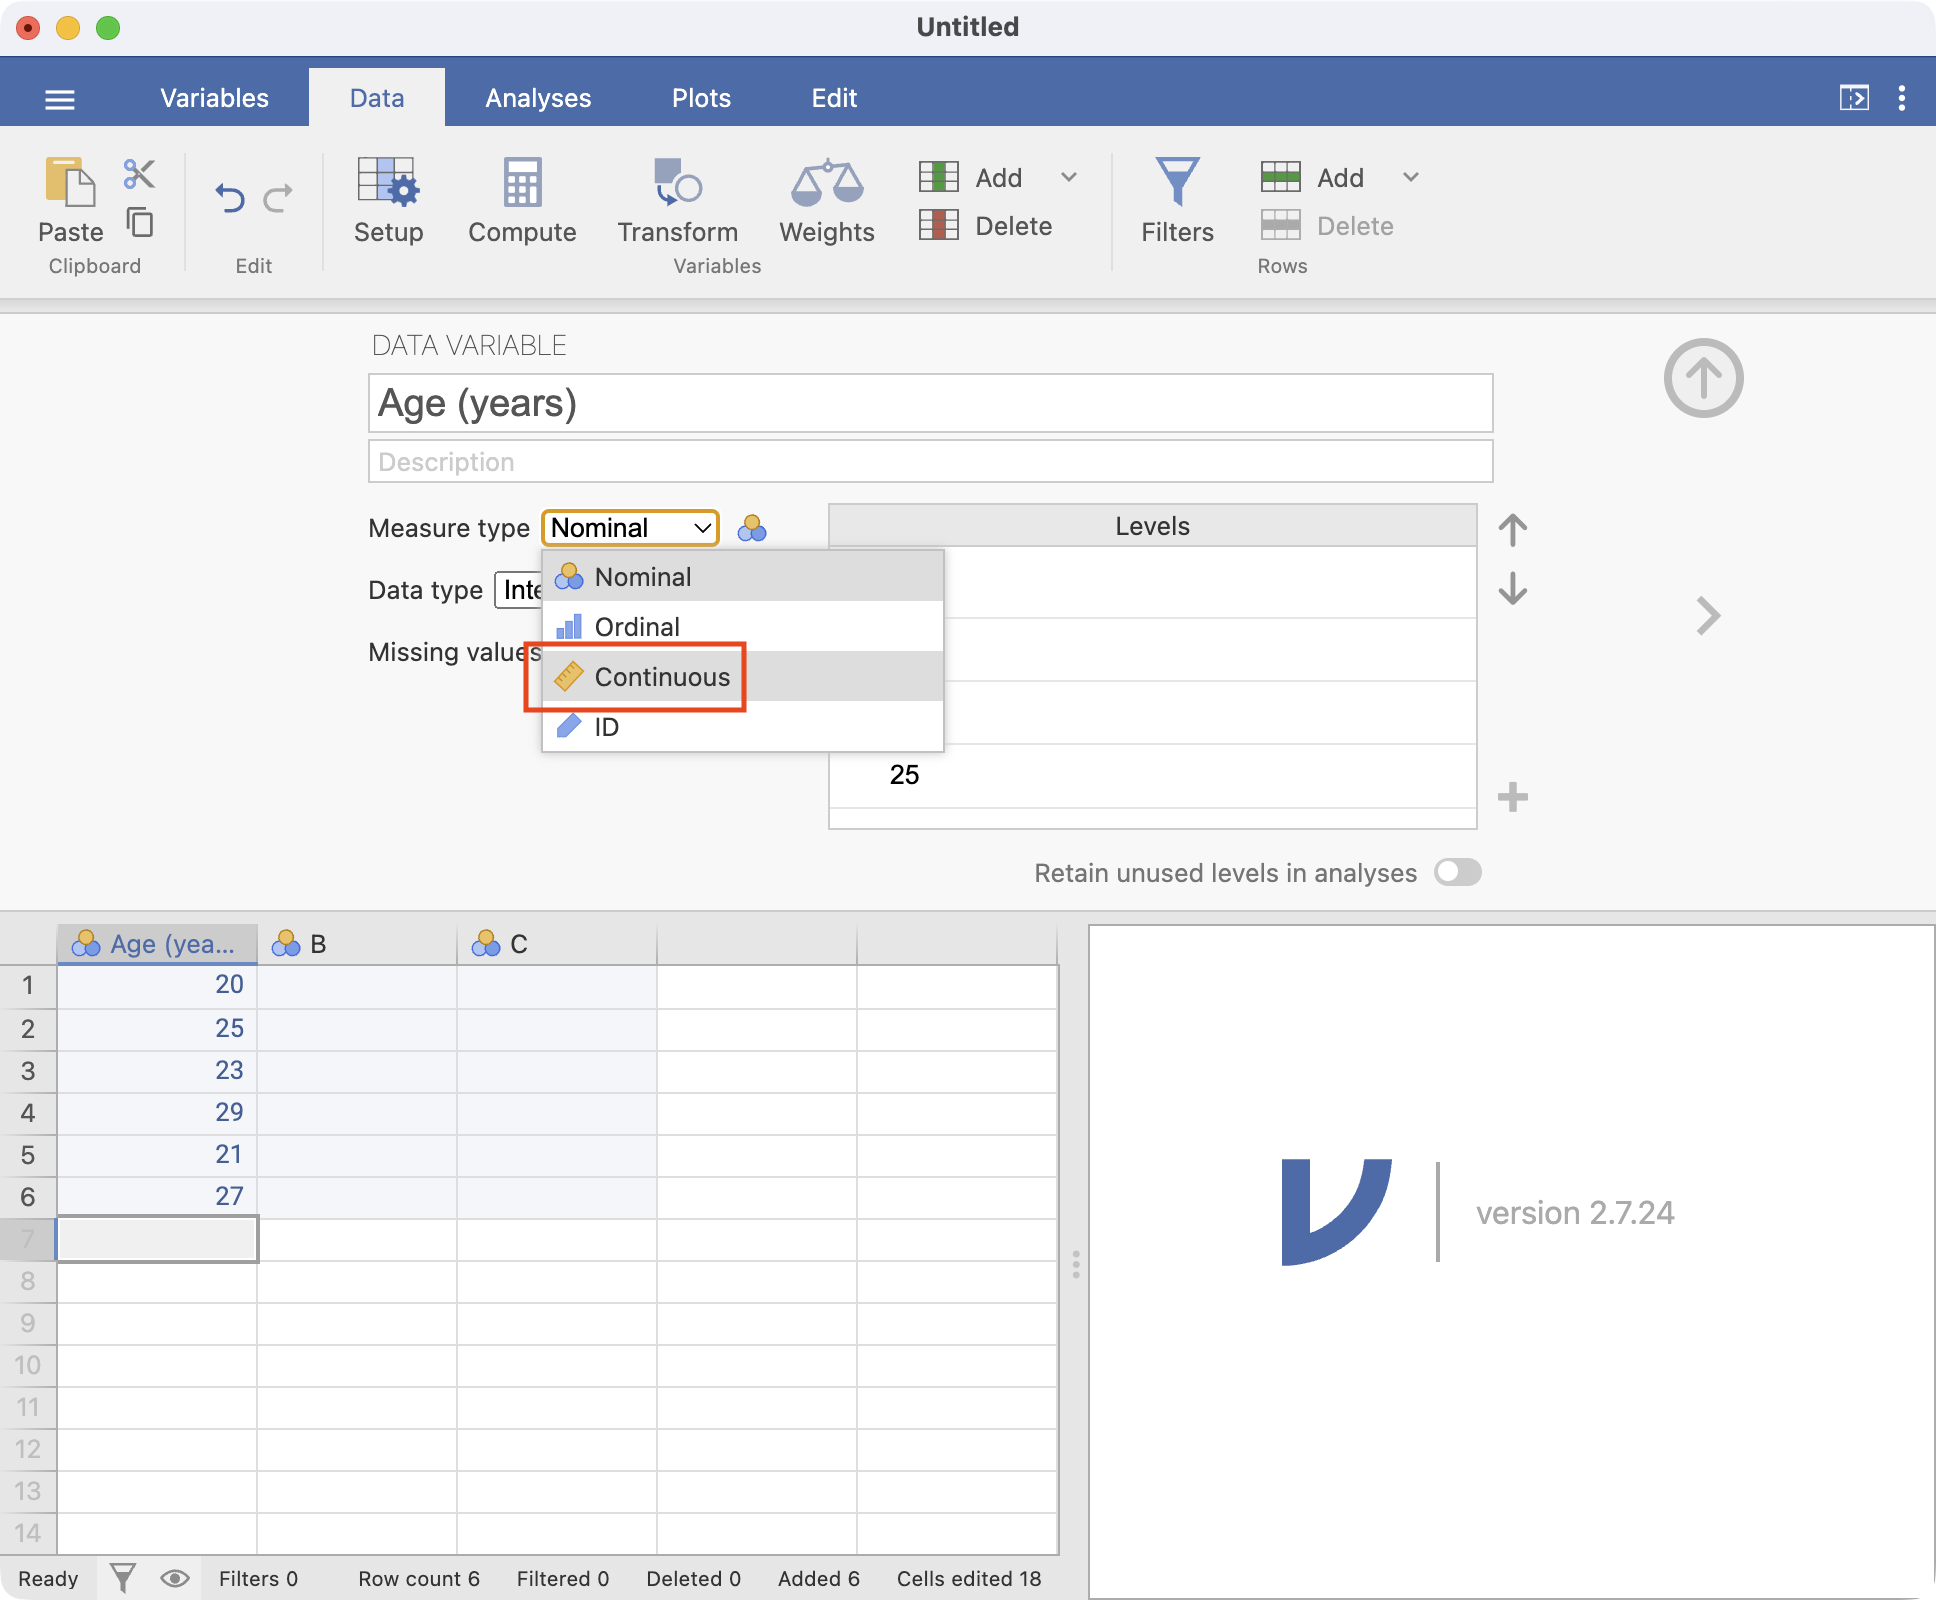
\includegraphics[keepaspectratio]{img/mod01/jamovi/variables-03.png}}

Once you have finished naming all your variables, you can click the
\textbf{Up} arrow to close the Setup tab to view the spreadsheet again.

jamovi is \emph{very} flexible with its naming convention, and allows
variable names that many other statistical packages would not allow.
Often, the only way to get publication quality graphs or tables is to
name your variables as completely as you can. However, I would recommend
the following conventions when choosing variable names in jamovi:

\begin{itemize}
\tightlist
\item
  try to keep your variable names relatively short;
\item
  variable names should start with a letter;
\item
  variable names are case-sensitive (so age, Age and AGE could represent
  three different variables)
\end{itemize}

\begin{tcolorbox}[enhanced jigsaw, arc=.35mm, bottomrule=.15mm, bottomtitle=1mm, breakable, colback=white, colbacktitle=quarto-callout-note-color!10!white, colframe=quarto-callout-note-color-frame, coltitle=black, left=2mm, leftrule=.75mm, opacityback=0, opacitybacktitle=0.6, rightrule=.15mm, title={TASK}, titlerule=0mm, toprule=.15mm, toptitle=1mm]

Rename the variable \texttt{A} with the name \texttt{Age\ (years)}, and
define age as a \emph{Continuous} variable.

\end{tcolorbox}

Now that we have entered our six ages, let's calculate the mean age.
Choose \textbf{Analyses \textgreater{} Exploration \textgreater{}
Descriptives}. The \textbf{Descriptives} dialog box will appear. Move
the variable \texttt{Age} into the \textbf{Variables} box by clicking
\texttt{Age\ (years)} and then clicking the right-arrow icon. The window
should appear as:

\pandocbounded{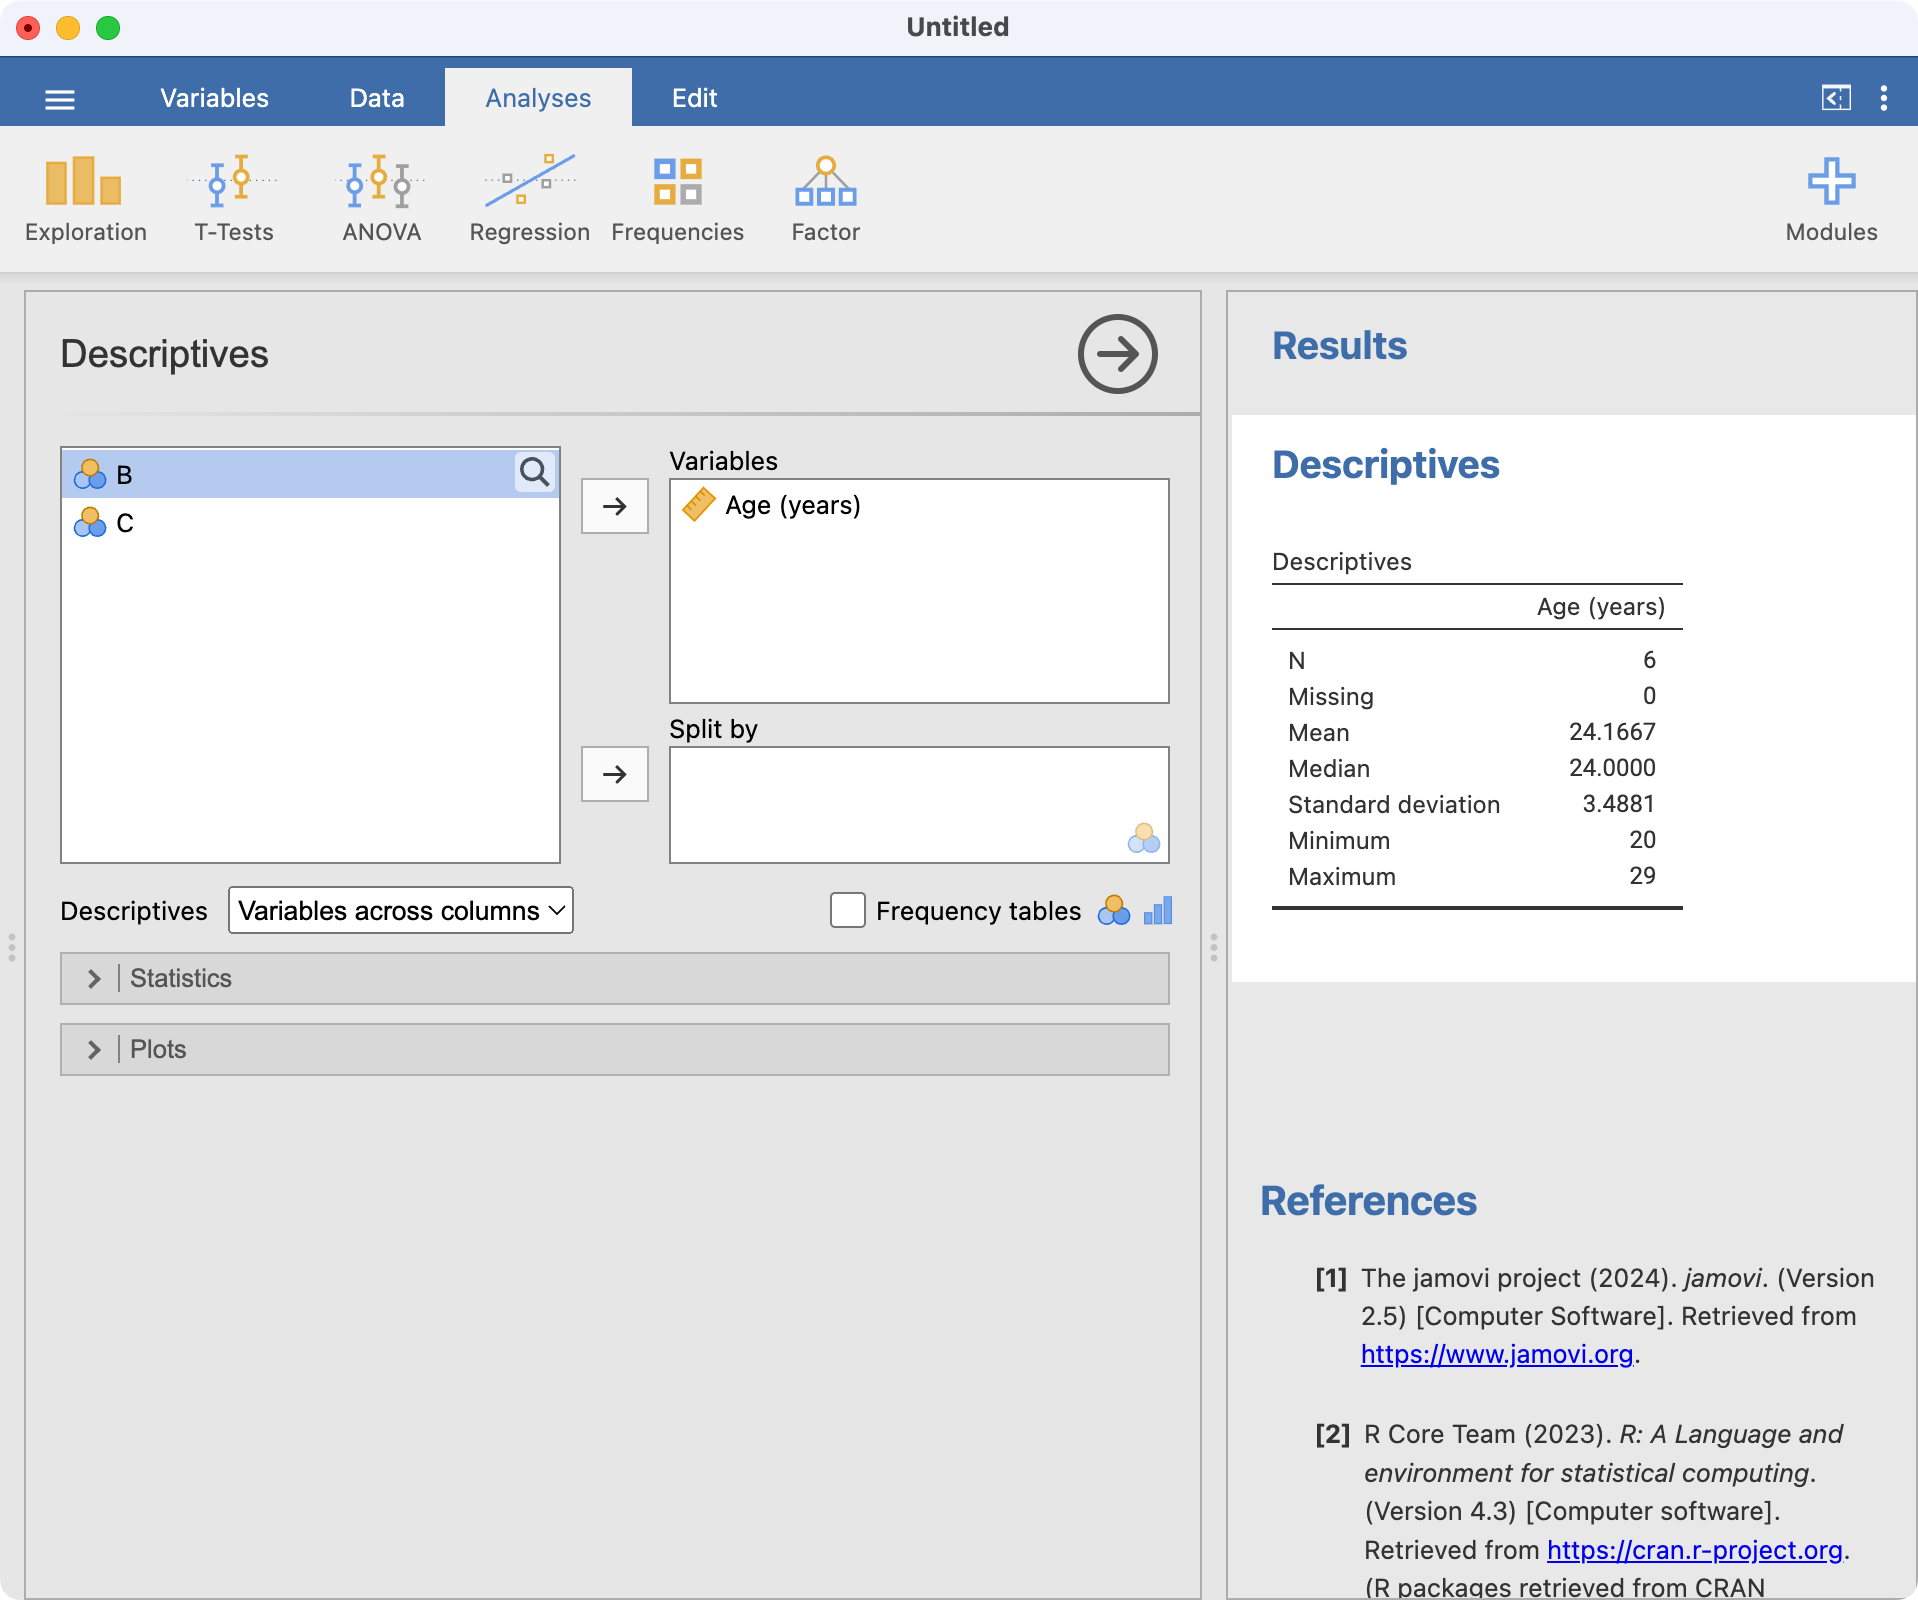
\includegraphics[keepaspectratio]{img/mod01/jamovi/simple-03.png}}

You can see the results of the analysis in the right-hand pane.

\begin{tcolorbox}[enhanced jigsaw, arc=.35mm, bottomrule=.15mm, bottomtitle=1mm, breakable, colback=white, colbacktitle=quarto-callout-note-color!10!white, colframe=quarto-callout-note-color-frame, coltitle=black, left=2mm, leftrule=.75mm, opacityback=0, opacitybacktitle=0.6, rightrule=.15mm, title={TASK}, titlerule=0mm, toprule=.15mm, toptitle=1mm]

Calculate summary statisitics for \texttt{Age\ (years)} and confirm:
there are 6 observations, with a mean age of 24.2 years, a standard
deviation of 3.49 years, a minimum of 20 and a maximum of 29 years.

\end{tcolorbox}

\subsection{The jamovi environment}\label{the-jamovi-environment}

Now that we have seen a simple example of how to use jamovi, let's
describe the jamovi environment. There are two main views in jamovi: the
\textbf{Spreadsheet} view, available by clicking the \textbf{Data} tab,
and the \textbf{Analysis} view, available by clicking the
\textbf{Analyses} tab. We will tend to use these two tabs through the
course.

The unique thing about jamovi is that \emph{all analyses are updated
whenever the data are changed in the spreadsheet}. While this can be
convinient, \emph{care must be taken not to make any unintended changes
to your data while in the spreadsheet view.}

jamovi also has a way of opening and saving data, using the three lines
in the upper-left corner:
\pandocbounded{
\includegraphics[keepaspectratio]{img/mod01/jamovi/three-lines.png}}.
This collection of commands lets you open data, save data and export
data and output.

\begin{tcolorbox}[enhanced jigsaw, arc=.35mm, bottomrule=.15mm, bottomtitle=1mm, breakable, colback=white, colbacktitle=quarto-callout-tip-color!10!white, colframe=quarto-callout-tip-color-frame, coltitle=black, left=2mm, leftrule=.75mm, opacityback=0, opacitybacktitle=0.6, rightrule=.15mm, title=\textcolor{quarto-callout-tip-color}{\faLightbulb}\hspace{0.5em}{Tip}, titlerule=0mm, toprule=.15mm, toptitle=1mm]

The \textbf{Special Import} command is hardly ever used. You should use
\textbf{Open} to open all types of data in jamovi.

\end{tcolorbox}

\section{Part 2: Obtaining summary statistics for continuous
data}\label{part-2-obtaining-summary-statistics-for-continuous-data}

In this exercise (spanning Modules 1 and 2), we will analyse data to
complete a descriptive table from a research study. The data come from a
study in primary biliary cirrhosis, a condition of the liver, from
Therneau and Grambsch (2010), Modeling Survival Data: Extending the Cox
Model. By the end of this exercise, we will have completed some of
Table~\ref{tbl-jamovi-t1}.

\begin{table}[h]

\caption{\label{tbl-jamovi-t1}Summary of 418 participants from the PBC
study (Therneau and Grambsch, 2000)}

\centering{

\centering
\begin{talltblr}[         %% tabularray outer open
entry=none,label=none,
note{}={* aspartate aminotransferase},
]                     %% tabularray outer close
{                     %% tabularray inner open
colspec={Q[]Q[]Q[]},
hline{2}={1-3}{solid, black, 0.05em},
hline{1}={1-3}{solid, black, 0.08em},
hline{14}={1-3}{solid, black, 0.08em},
}                     %% tabularray inner close
Characteristic &   & Summary \\
Age (years) &   & Mean (SD) or Median [IQR] \\
Sex & Male & n (\%) \\
& Female & n (\%) \\
AST* (U/ml) &   & Mean (SD) or Median [IQR] \\
Serum bilirubin &   & Mean (SD) or Median [IQR] \\
Stage & I & n (\%) \\
& II & n (\%) \\
& III & n (\%) \\
& IIIV & n (\%) \\
Vital status at study end & Alive: no transplant & n (\%) \\
& Alive: transplant & n (\%) \\
& Deceased & n (\%) \\
\end{talltblr}

}

\end{table}%

\begin{tcolorbox}[enhanced jigsaw, arc=.35mm, bottomrule=.15mm, bottomtitle=1mm, breakable, colback=white, colbacktitle=quarto-callout-note-color!10!white, colframe=quarto-callout-note-color-frame, coltitle=black, left=2mm, leftrule=.75mm, opacityback=0, opacitybacktitle=0.6, rightrule=.15mm, title={TASK}, titlerule=0mm, toprule=.15mm, toptitle=1mm]

Download the table shell, saved as \texttt{PBC\ Table1.docx}, and the
information file called \texttt{mod01\_pbc\_info.txt}.

\end{tcolorbox}

\subsection{Opening a data file}\label{opening-a-data-file}

Typing data directly into jamovi is not common; we usually open data
that have been saved as a file. jamovi can open many types of files,
including text (txt), comma separated (csv), Microsoft Excel (xlsx), R
(rds), Stata (dta) and more. Here, we will open a dataset that has been
stored as an R data file (which has the \texttt{.rds} suffix).

\begin{tcolorbox}[enhanced jigsaw, arc=.35mm, bottomrule=.15mm, bottomtitle=1mm, breakable, colback=white, colbacktitle=quarto-callout-note-color!10!white, colframe=quarto-callout-note-color-frame, coltitle=black, left=2mm, leftrule=.75mm, opacityback=0, opacitybacktitle=0.6, rightrule=.15mm, title={TASK}, titlerule=0mm, toprule=.15mm, toptitle=1mm]

Load the sample data set called \texttt{mod01\_pbc.rds} into jamovi
using the following steps:

\begin{enumerate}
\def\labelenumi{\arabic{enumi}.}
\item
  Locate the data set called \texttt{mod01\_pbc.rds}. Click the file to
  download it, and then save it in a folder you will be able to locate
  later - for example, your OneDrive folder.
\item
  In jamovi, click the three-bar icon, then choose \textbf{Open}. jamovi
  usually searches in the most recently used folder, so most times you
  will need to \textbf{click Browse}. Browse to where you stored the
  dataset and click \textbf{Open}.
\end{enumerate}

Confirm that there are 418 rows by examining the \textbf{Row count} at
the bottom of the screen.

Examine the \texttt{pbc\_info.txt} file for a description of each
variable.

\end{tcolorbox}

\subsection{Assigning meaningful variable
names}\label{assigning-meaningful-variable-names}

As we saw earlier, jamovi has can allow quite useful variable names,
which will appear when creating output. For example, the variable
entered as bili could be named \texttt{Serum\ bilirubin\ (mg/dl)}.

\begin{tcolorbox}[enhanced jigsaw, arc=.35mm, bottomrule=.15mm, bottomtitle=1mm, breakable, colback=white, colbacktitle=quarto-callout-note-color!10!white, colframe=quarto-callout-note-color-frame, coltitle=black, left=2mm, leftrule=.75mm, opacityback=0, opacitybacktitle=0.6, rightrule=.15mm, title={TASK}, titlerule=0mm, toprule=.15mm, toptitle=1mm]

Assign meaningful variable names to the variables used in Table 1. You
should to refer to the file \texttt{pbc\_info.txt} to determine what
each variable represents.

\end{tcolorbox}

\subsection{Summarising continuous
variables}\label{summarising-continuous-variables}

As we saw in Part 1, continuous variables can be summarised using
\textbf{Analyses \textgreater{} Exploration}. There are three continuous
variables that we would like to summarise: age, AST and serum bilirubin.
Each of these can be listed in the \textbf{Exploration} dialog box, as
shown below. The summaries are calculated automatically:

\pandocbounded{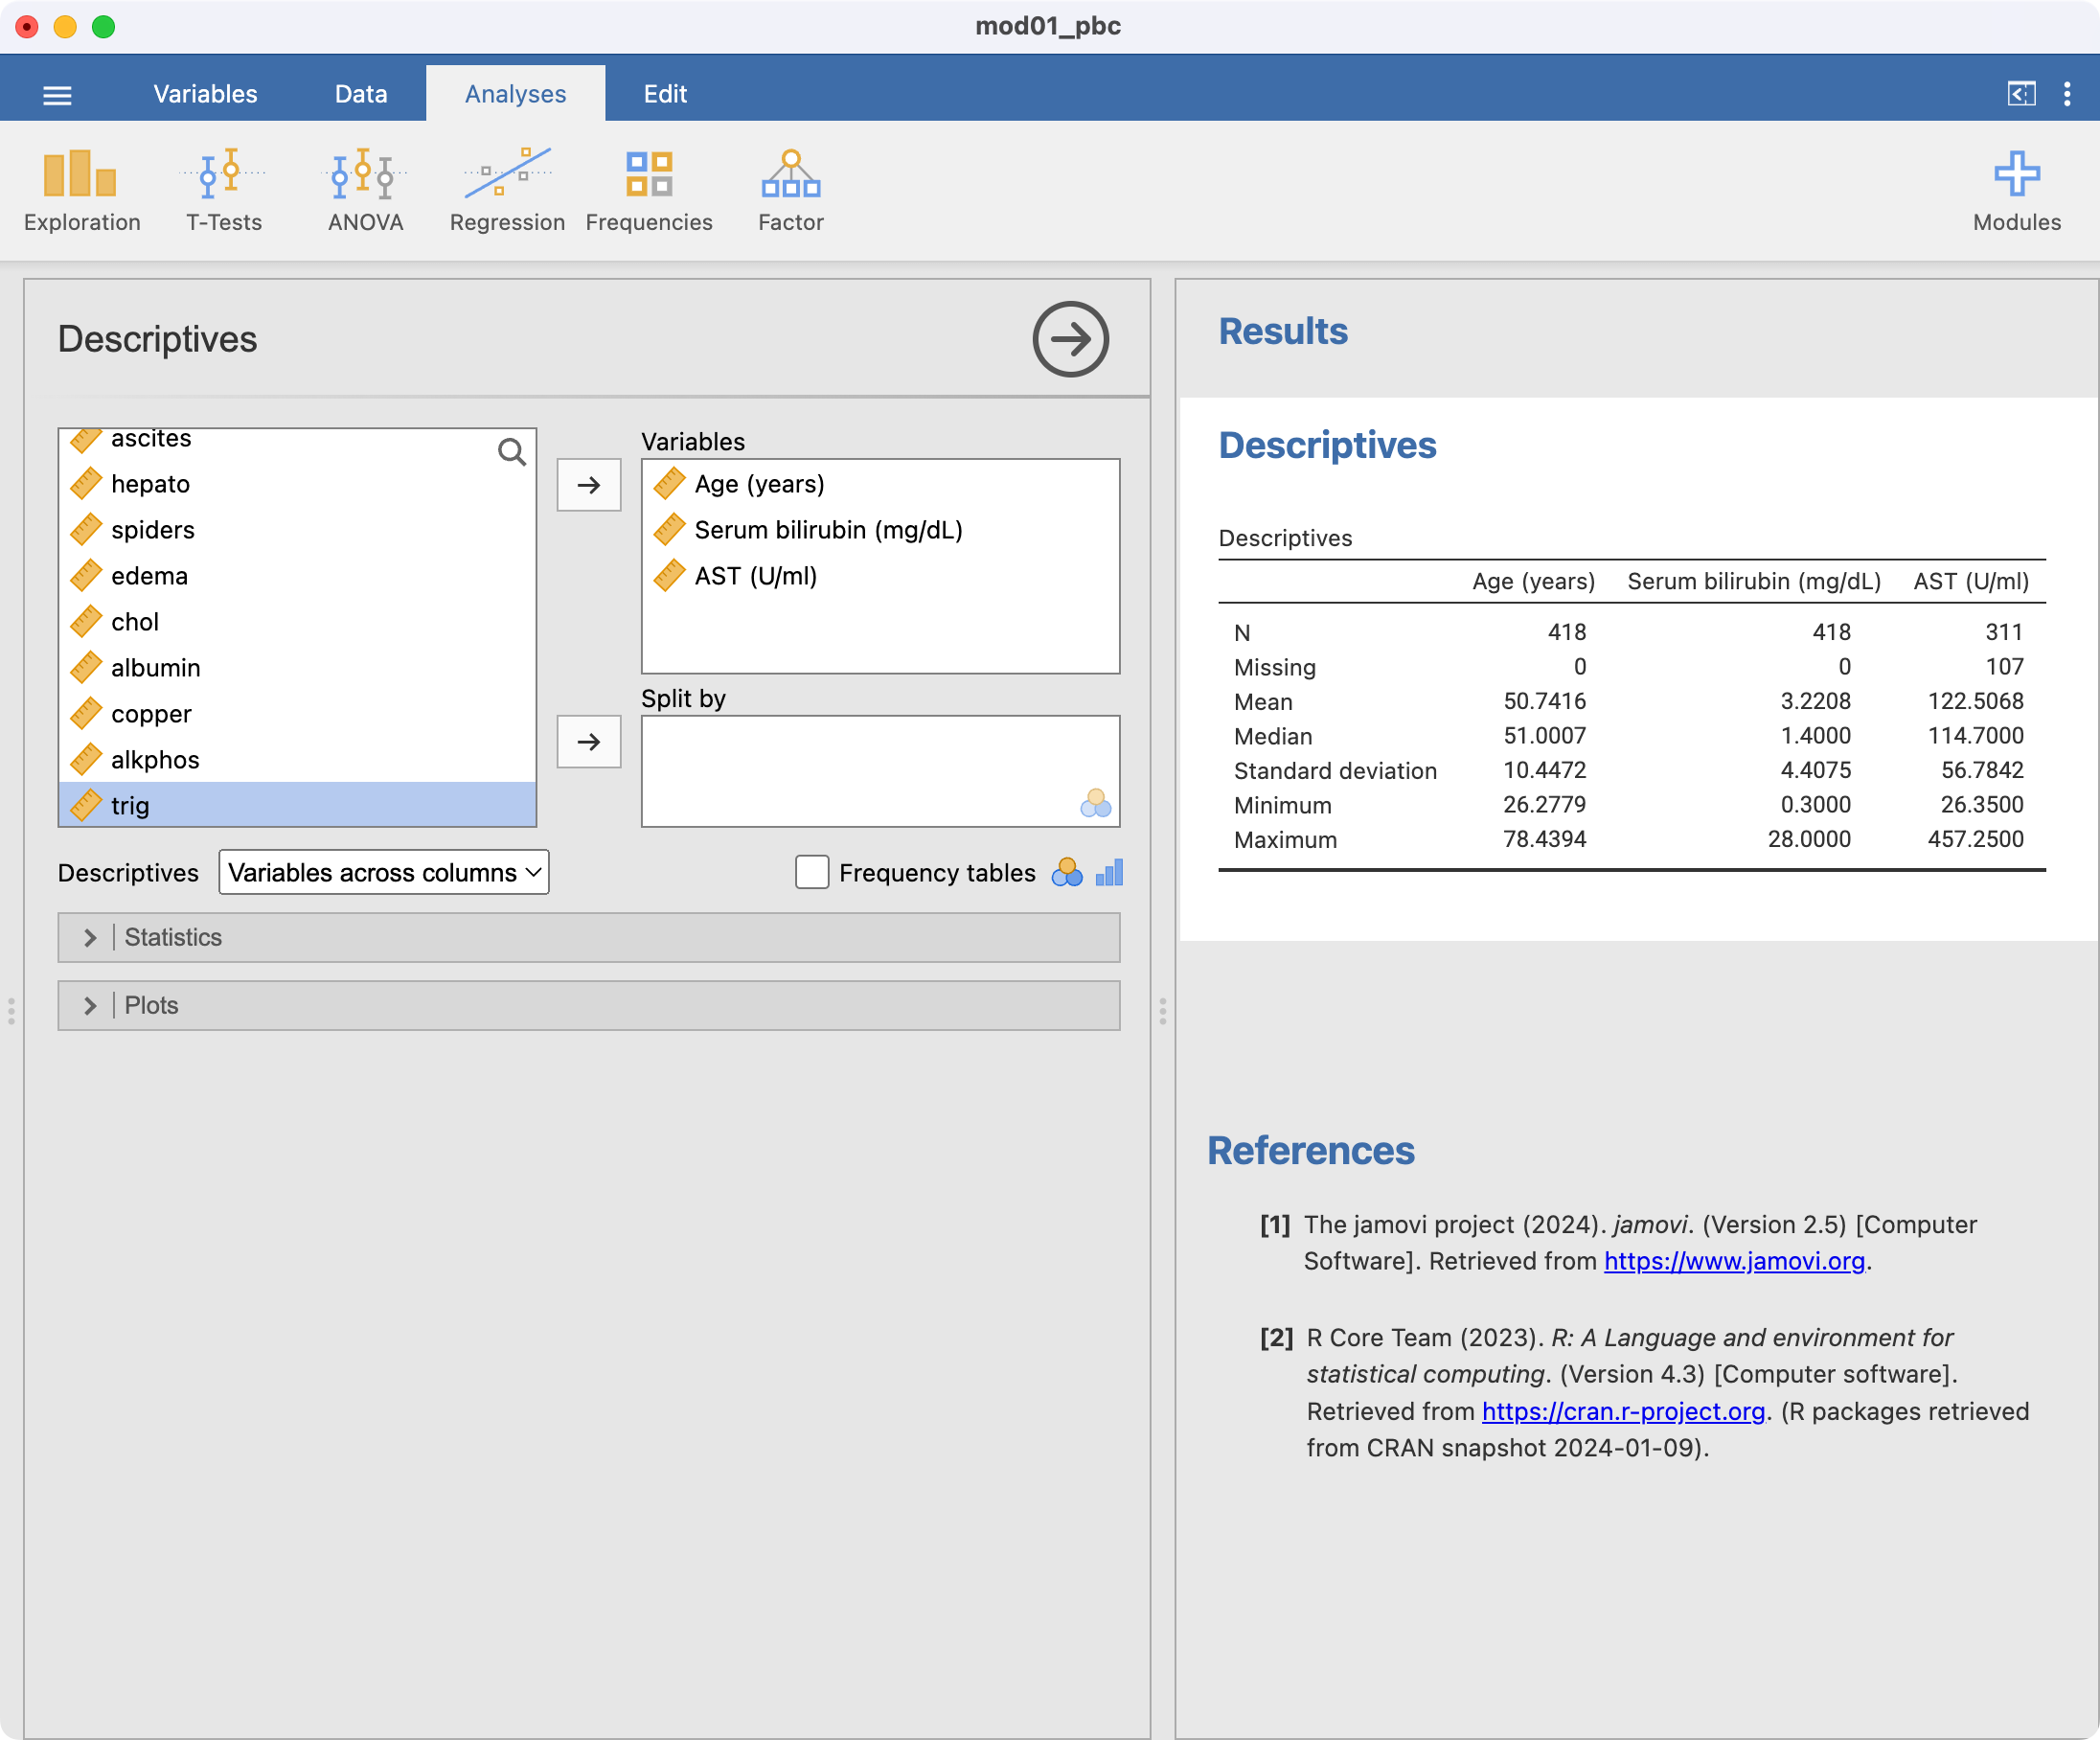
\includegraphics[keepaspectratio]{img/mod01/jamovi/summ-01.png}}

By default, the exploration command presents the number of observations,
the number of missing observations, the mean, median, standard
deviation, minimum and maximum. We may be interested in obtaining the
interquartile range as well, so we select the \textbf{Statistics} arrow,
and choose \textbf{Percentiles}:

\pandocbounded{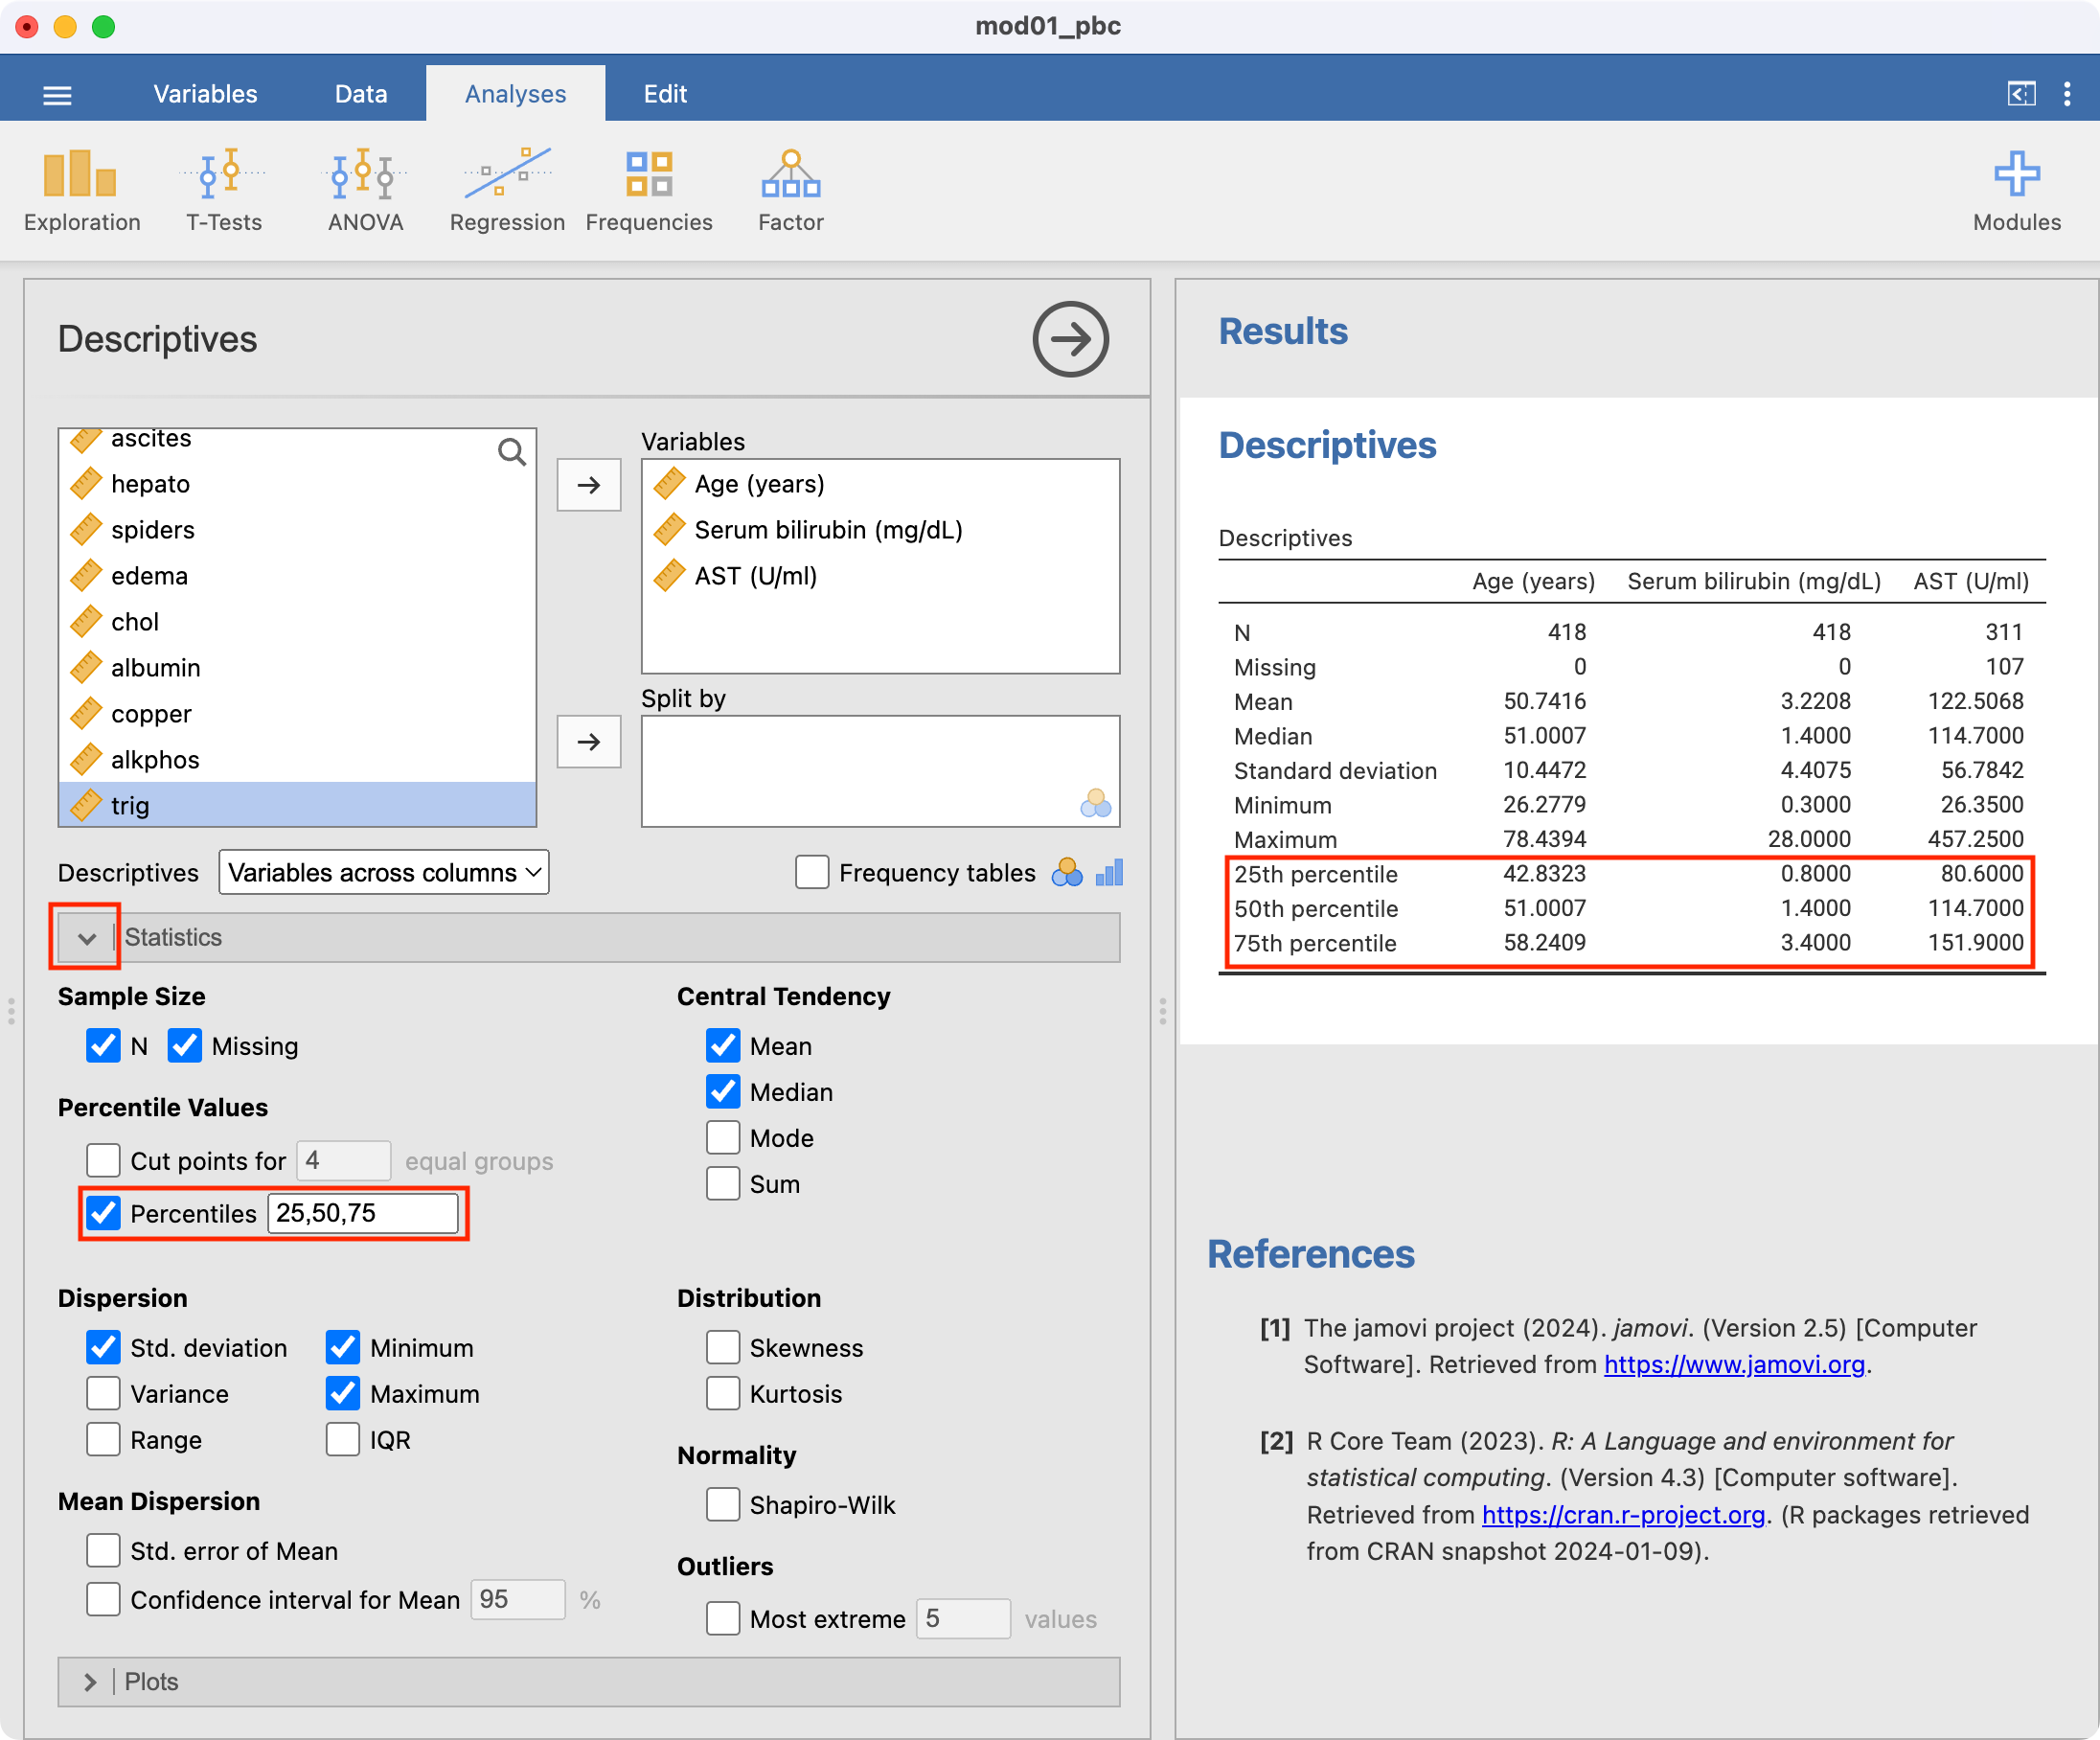
\includegraphics[keepaspectratio]{img/mod01/jamovi/summ-02.png}}

For each of our three continuous variables, we need to decide whether to
present the mean and standard deviation, or the median and interquartile
range. This decision can be made after examining a density plot (and
perhaps a boxplot) for each variable.

\subsection{Producing a density plot}\label{producing-a-density-plot}

To produce a density plot, click the arrow next to \textbf{Plots} and
choose \textbf{Density}. Plots will be produced for each variable listed
in the \textbf{Variables} box. The density plots will be produced one
after another, but they have been presented horizontally here:

\pandocbounded{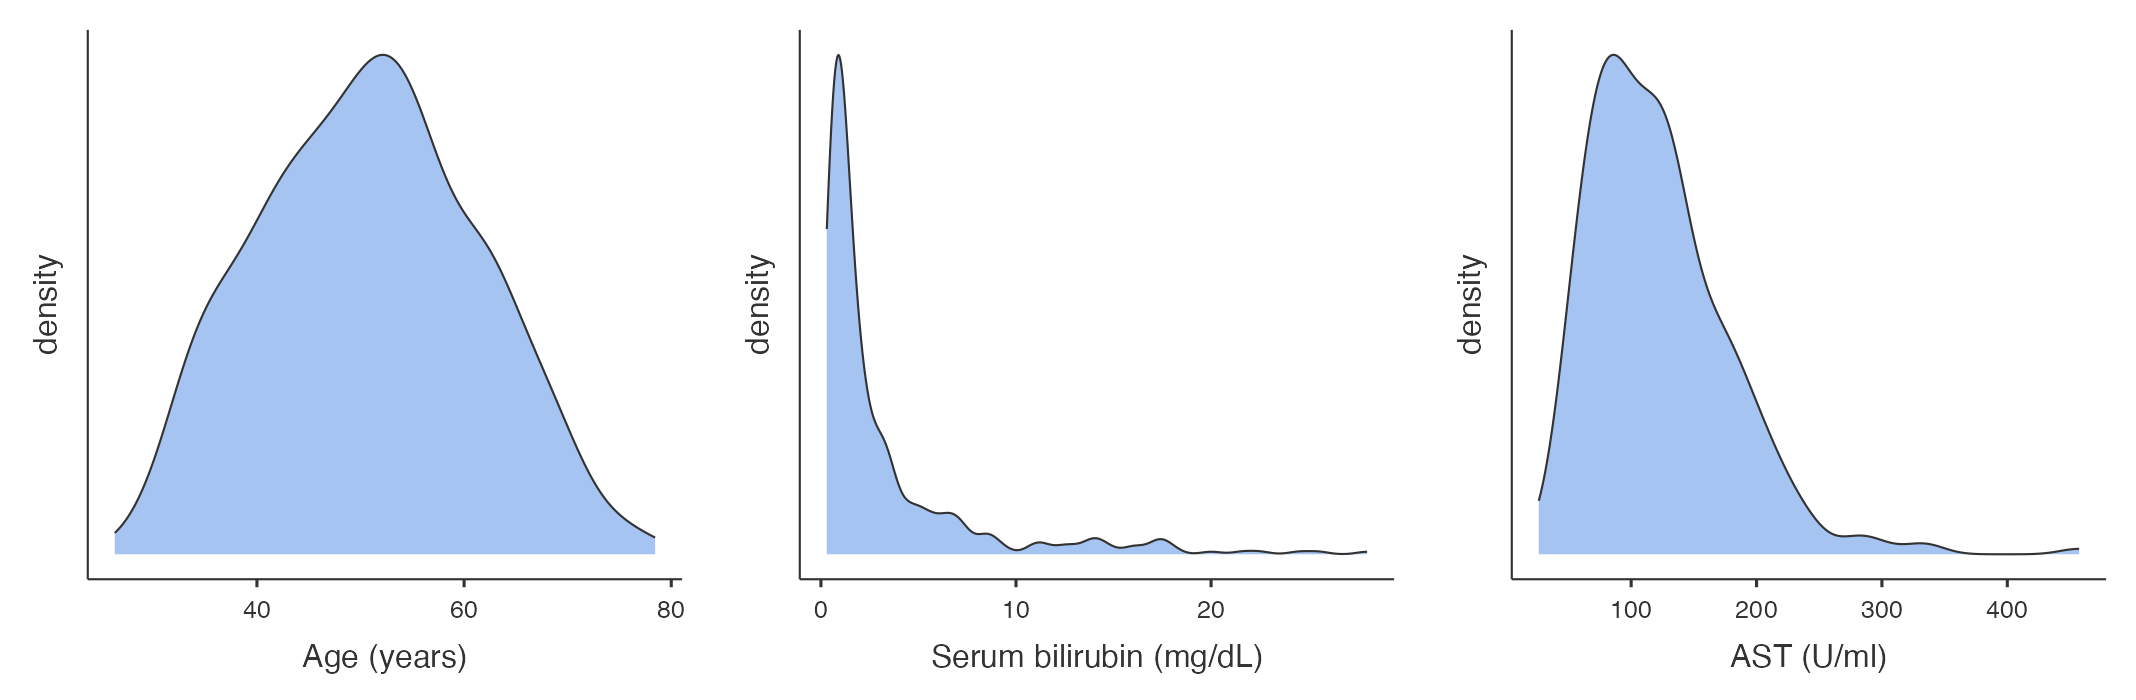
\includegraphics[keepaspectratio]{img/mod01/jamovi/densplot-all.png}}

\subsection{Producing a boxplot}\label{producing-a-boxplot}

Producing boxplots is done by ticking the \textbf{Box plot} box. By
default, jamovi labels each of the points that it considers to be an
outlier with its row number; this can be turned off if desired.

\begin{tcolorbox}[enhanced jigsaw, arc=.35mm, bottomrule=.15mm, bottomtitle=1mm, breakable, colback=white, colbacktitle=quarto-callout-note-color!10!white, colframe=quarto-callout-note-color-frame, coltitle=black, left=2mm, leftrule=.75mm, opacityback=0, opacitybacktitle=0.6, rightrule=.15mm, title={TASK}, titlerule=0mm, toprule=.15mm, toptitle=1mm]

Obtain density plots and boxplots for age, AST and bilirubin.

Based on these plots, decide whether the mean or the median is the
appropriate summary to use for each variable.

\end{tcolorbox}

\subsection{Saving your work from
jamovi}\label{saving-your-work-from-jamovi}

Now that you have made some changes to the pbc data and conducted some
analyses, it is good practice to save your work. jamovi uses its own
file format to save \textbf{both data and output}, using files with .omv
suffix. All changes to your data will be saved, as well as all existing
output. However, work saved by jamovi will only be able to be opened by
jamovi - you will not easily be able to share your data or your output
with colleagues who do not have jamovi. To save a jamovi session, choose
\textbf{Save} in the three-lines tab.

If you want to share work with colleagues who do not have jamovi, you
can use \textbf{Export} to save your data in another file format
(recognising that variable and value labels will not be exported), or
save your output as a \texttt{pdf} or \texttt{html} file.

\subsection{Copying output from
jamovi}\label{copying-output-from-jamovi}

An easy way to share output between your colleagues is to copy the
output into a word processor package (e.g.~Microsoft Word). To copy
output from jamovi, you can \textbf{right-click}\footnote{\textbf{Windows}

  \begin{itemize}
  \tightlist
  \item
    Click the right mouse button to open a context menu
  \item
    Shows options relevant to what you clicked on (copy, export, add
    note)
  \end{itemize}

  \textbf{Mac}

  \begin{itemize}
  \tightlist
  \item
    Two-button mouse: Press right button
  \item
    One-button mouse/trackpad: Hold Control (Ctrl) while clicking
  \item
    Functions the same as Windows - shows context-specific options
  \end{itemize}} the output with your mouse, and choose \textbf{Export}.
This will copy the output as plain text for pasting into a Word
document. If you select a single table for copying, you can also
\textbf{Copy table} or \textbf{Copy table as HTML}. Whichever way you
copy output into Word, you will need to make sure your output conforms
with all style guides required for your final publication.

\begin{tcolorbox}[enhanced jigsaw, arc=.35mm, bottomrule=.15mm, bottomtitle=1mm, breakable, colback=white, colbacktitle=quarto-callout-note-color!10!white, colframe=quarto-callout-note-color-frame, coltitle=black, left=2mm, leftrule=.75mm, opacityback=0, opacitybacktitle=0.6, rightrule=.15mm, title={TASK}, titlerule=0mm, toprule=.15mm, toptitle=1mm]

Complete Table 1 for continuous variables using the output generated in
this exercise. You should decide on whether to present continuous
variables by their means or medians, and present the most appropriate
measure of spread. Include footnotes to indicate if any variables
contain missing observations.

\end{tcolorbox}

\section{Setting a value to missing}\label{setting-a-value-to-missing}

As we saw in Section~\ref{sec-eda-cts}, it is important to explore our
data to identify any unusual observations. If an error is found, the
best method for correcting the error is to go back to the original data
e.g.~the hard copy questionnaire, to obtain the original value, entering
the correct value into jamovi. If the original data is not available or
the original data is also incorrect, the erroneous value is often
excluded from the dataset.

Consider a sample dataset: \texttt{mod01\_weight\_1000.rds}, which
contains the weights of 1000 people. A density plot and a boxplot should
be examined before we start analysing these data:

\begin{figure}

\begin{minipage}[t]{0.50\linewidth}

\raisebox{-\height}{

\pandocbounded{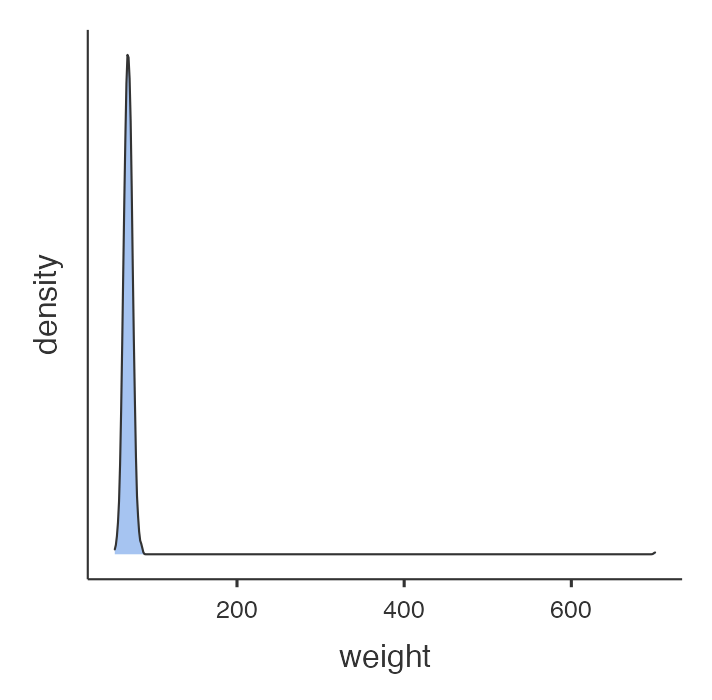
\includegraphics[keepaspectratio]{img/mod01/jamovi/densplot-weight.png}}

}

\end{minipage}%
%
\begin{minipage}[t]{0.50\linewidth}

\raisebox{-\height}{

\pandocbounded{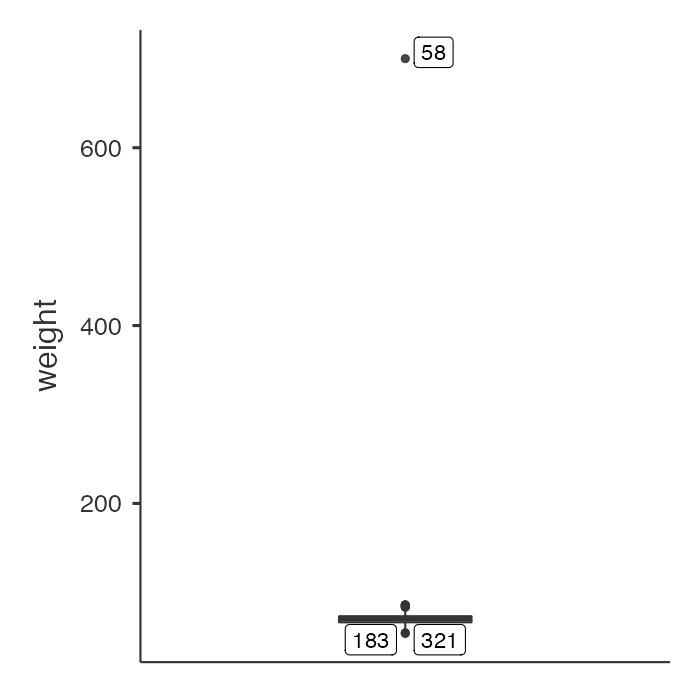
\includegraphics[keepaspectratio]{img/mod01/jamovi/boxplot-weight.png}}

}

\end{minipage}%

\end{figure}%

There is a clear outlying point shown in the boxplot. Although not
obvious, the same point is shown in the density plot as a small blip
around 700kg. Obviously this point is unusual, and we should
investigate. You will need to decide if any usual values are a data
entry error or are biologically plausible. If an extreme value or
``outlier'', is biologically plausible, it should be included in all
analyses.

Notice the boxed number in the boxplot: this is the record number in
jamovi's spreadsheet. Click \textbf{Data} to view the spreadsheet, and
scroll to record number 58:

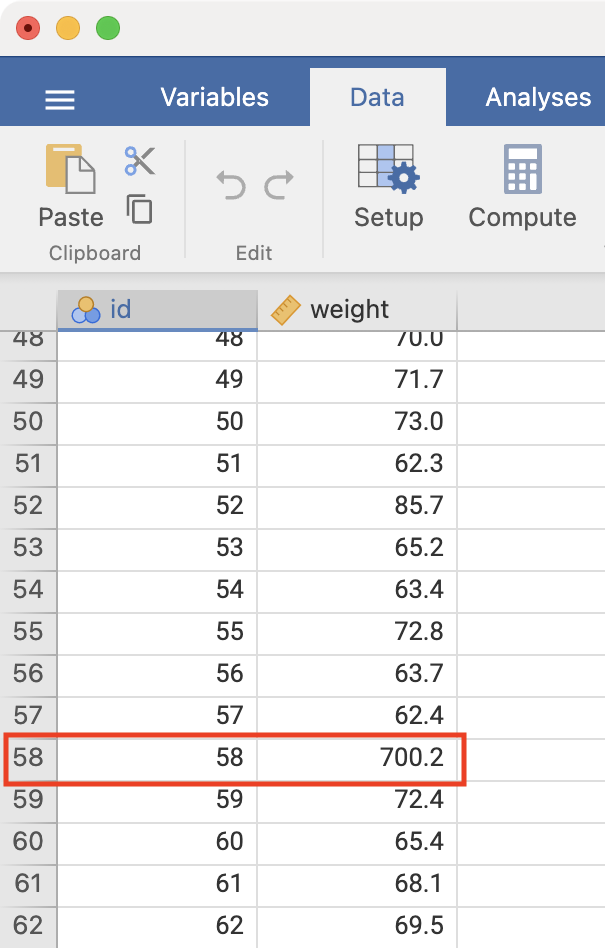
\includegraphics[width=0.4\linewidth,height=\textheight,keepaspectratio]{img/mod01/jamovi/outlier.png}

We see that there is a very high value of 700.2kg. A value as high as
700kg is likely to be a data entry error (e.g.~error in entering an
extra zero) and is not a plausible weight value. Here, \textbf{you
should check your original data}.

If you do not have access to the original data, it would be safest to
set this value as missing. You do change this in jamovi by clicking the
datapoint and pressing \textbf{Delete} or \textbf{Backspace}. This has
set this weight to missing.

\textbf{Note:} if an extreme value lies within the range of biological
possibility it should not be set to missing.

The same process could be used to replace the incorrect value with the
correct value. For example, if you do source the original medical
records, you might find that the original weight was recorded in medical
records as 70.2kg. We could use the same process to replace 700.2 by
70.2 by entering the correct value in the cell.

Once you have checked your data for errors, you are ready to start
analysing your data.

\begin{tcolorbox}[enhanced jigsaw, arc=.35mm, bottomrule=.15mm, bottomtitle=1mm, breakable, colback=white, colbacktitle=quarto-callout-important-color!10!white, colframe=quarto-callout-important-color-frame, coltitle=black, left=2mm, leftrule=.75mm, opacityback=0, opacitybacktitle=0.6, rightrule=.15mm, title=\textcolor{quarto-callout-important-color}{\faExclamation}\hspace{0.5em}{Important}, titlerule=0mm, toprule=.15mm, toptitle=1mm]

Whenever you start changing data in jamovi, you should \textbf{always
keep an original, unedited copy of your data.} You can do this using
\textbf{Save As} to save your edited work, leaving the original data
unchanged.

\end{tcolorbox}

\newpage{}

\bookmarksetup{startatroot}

\chapter*{An introduction to R and
RStudio}\label{an-introduction-to-r-and-rstudio}
\addcontentsline{toc}{chapter}{An introduction to R and RStudio}

\markboth{An introduction to R and RStudio}{An introduction to R and
RStudio}

\section*{Learning outcomes}\label{learning-outcomes-2}
\addcontentsline{toc}{section}{Learning outcomes}

\markright{Learning outcomes}

By the end of this Module, you will be able to:

\begin{itemize}
\tightlist
\item
  understand the difference between R and RStudio
\item
  navigate the RStudio interface
\item
  input and import data into R
\item
  use R to summarise data
\item
  perform basic data transformations
\item
  understand the difference between saving R data and saving R output
\item
  copy R output to a standard word processing package
\end{itemize}

\section{Part 1: An introduction to
R}\label{part-1-an-introduction-to-r}

``R is a language and environment for statistical computing and
graphics.'' \href{https://www.r-project.org/about.html}{Link}. It is an
open-source programming language, used mainly for statistics (including
biostatistics) and data science.

The aim of these notes is to introduce the R language within the RStudio
environment, and to introduce the commands and procedures that are
directly relevant to this course. There is so much more to R than we can
cover in these notes. Relevant information will be provided throughout
the course, and we will provide further references that you can explore
if you are interested.

\subsection{R vs RStudio}\label{r-vs-rstudio}

At its heart, R is a programming language. When you install R on your
computer, you are installing the language and its resources, as well as
a very basic interface for using R. You can write and run R code using
the basic R app, but it's not recommended.

RStudio is an ``Integrated Development Environment'' that runs R while
also providing useful tools to help you write code and analyse data. You
can think of R as an engine which does the work, and RStudio as a car
that uses the engine, but also provides useful tools like GPS navigation
and reversing cameras that help you drive.

Note: even though we recommend that you use RStudio, you still need
install R. \textbf{RStudio will not run without R installed.}

In summary, we recommend you use RStudio to write R code.

\subsection{Installing R and RStudio}\label{installing-r-and-rstudio}

\subsubsection{To install R on your
computer}\label{to-install-r-on-your-computer}

\begin{enumerate}
\def\labelenumi{\arabic{enumi}.}
\item
  Download the R installer from:

  \begin{enumerate}
  \def\labelenumii{\alph{enumii}.}
  \tightlist
  \item
    for Windows: \url{https://cran.r-project.org/bin/windows/base/}
  \item
    for MacOS: \url{https://cran.r-project.org/bin/macosx/}
  \end{enumerate}
\item
  Install R by running the installer and following the installation
  instructions. The default settings are fine.
\item
  Open the R program. You should see a screen similar to below:
\end{enumerate}

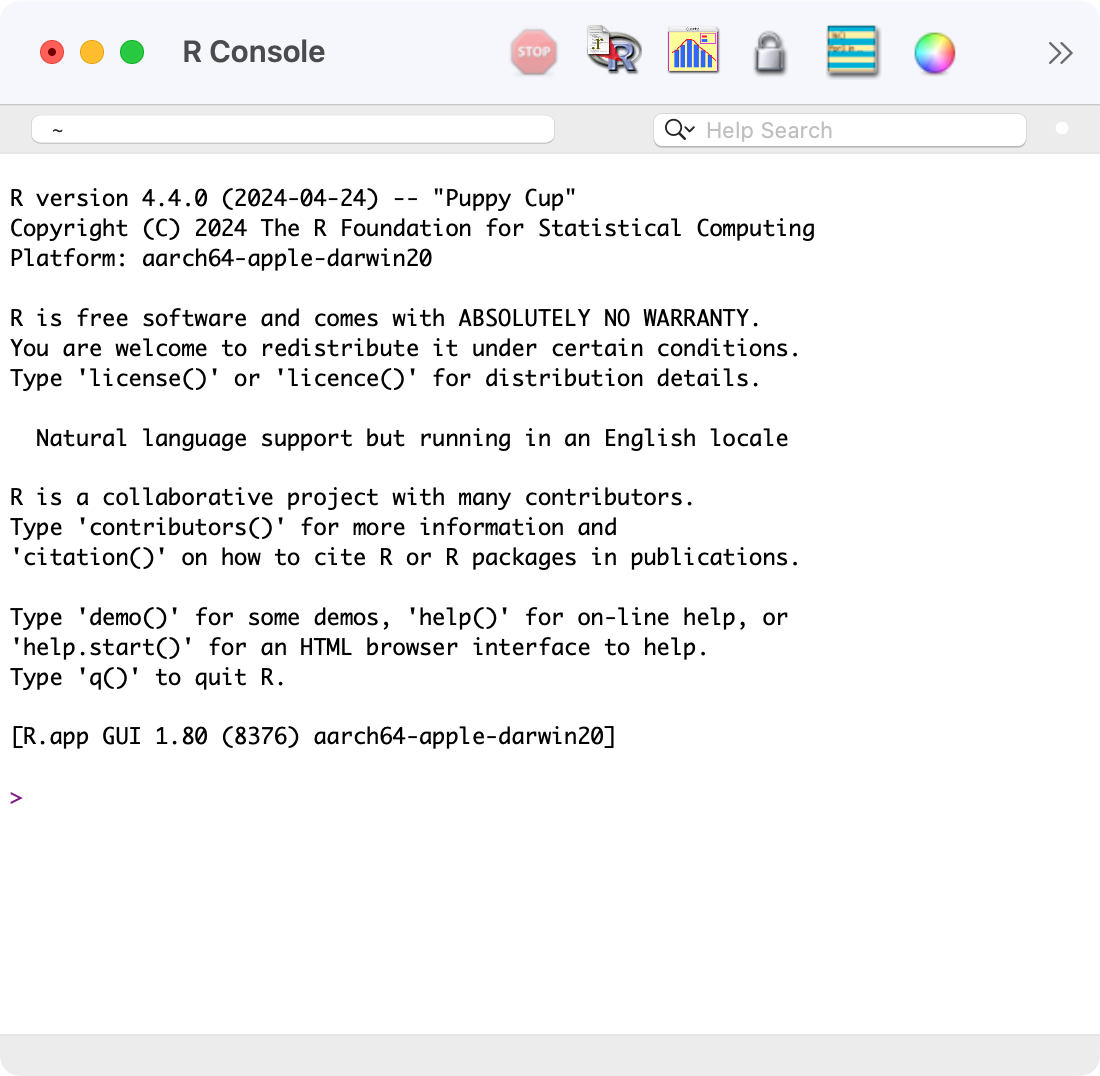
\includegraphics[width=0.8\linewidth,height=\textheight,keepaspectratio]{img/mod01/R-screenshot.png}

Near the bottom of the R screen, you will find the ``\textgreater{}''
symbol which represents R's command line; this is where you can type
your R commands for processing. If you type \texttt{1\ +\ 2} into the
command line and then hit enter you should get:

\texttt{{[}1{]}\ 3}

This is R performing your calculation, with the \texttt{{[}1{]}}
indicating that the solution to \texttt{1\ +\ 2} is a single number (the
number 3).

At this point, close R - we will not interact with R like this in the
future. You can close R by typing \texttt{quit()} at the command prompt,
followed by the return key, or in the usual way of closing an
application in your operating system. There is no need to save anything
here if prompted.

\subsubsection{To install RStudio on your
computer}\label{to-install-rstudio-on-your-computer}

\begin{enumerate}
\def\labelenumi{\arabic{enumi}.}
\tightlist
\item
  Make sure you have already installed R, and verified that it is
  working.
\item
  Download the RStudio desktop installer at:
  \url{https://posit.co/download/rstudio-desktop/}. The website should
  detect your operating system and link to the appropriate installer for
  your computer.
\item
  Install RStudio by running the installer and following the
  installation instructions. The default settings are fine.
\item
  Open RStudio, which will appear similar to the screenshot below:
\end{enumerate}

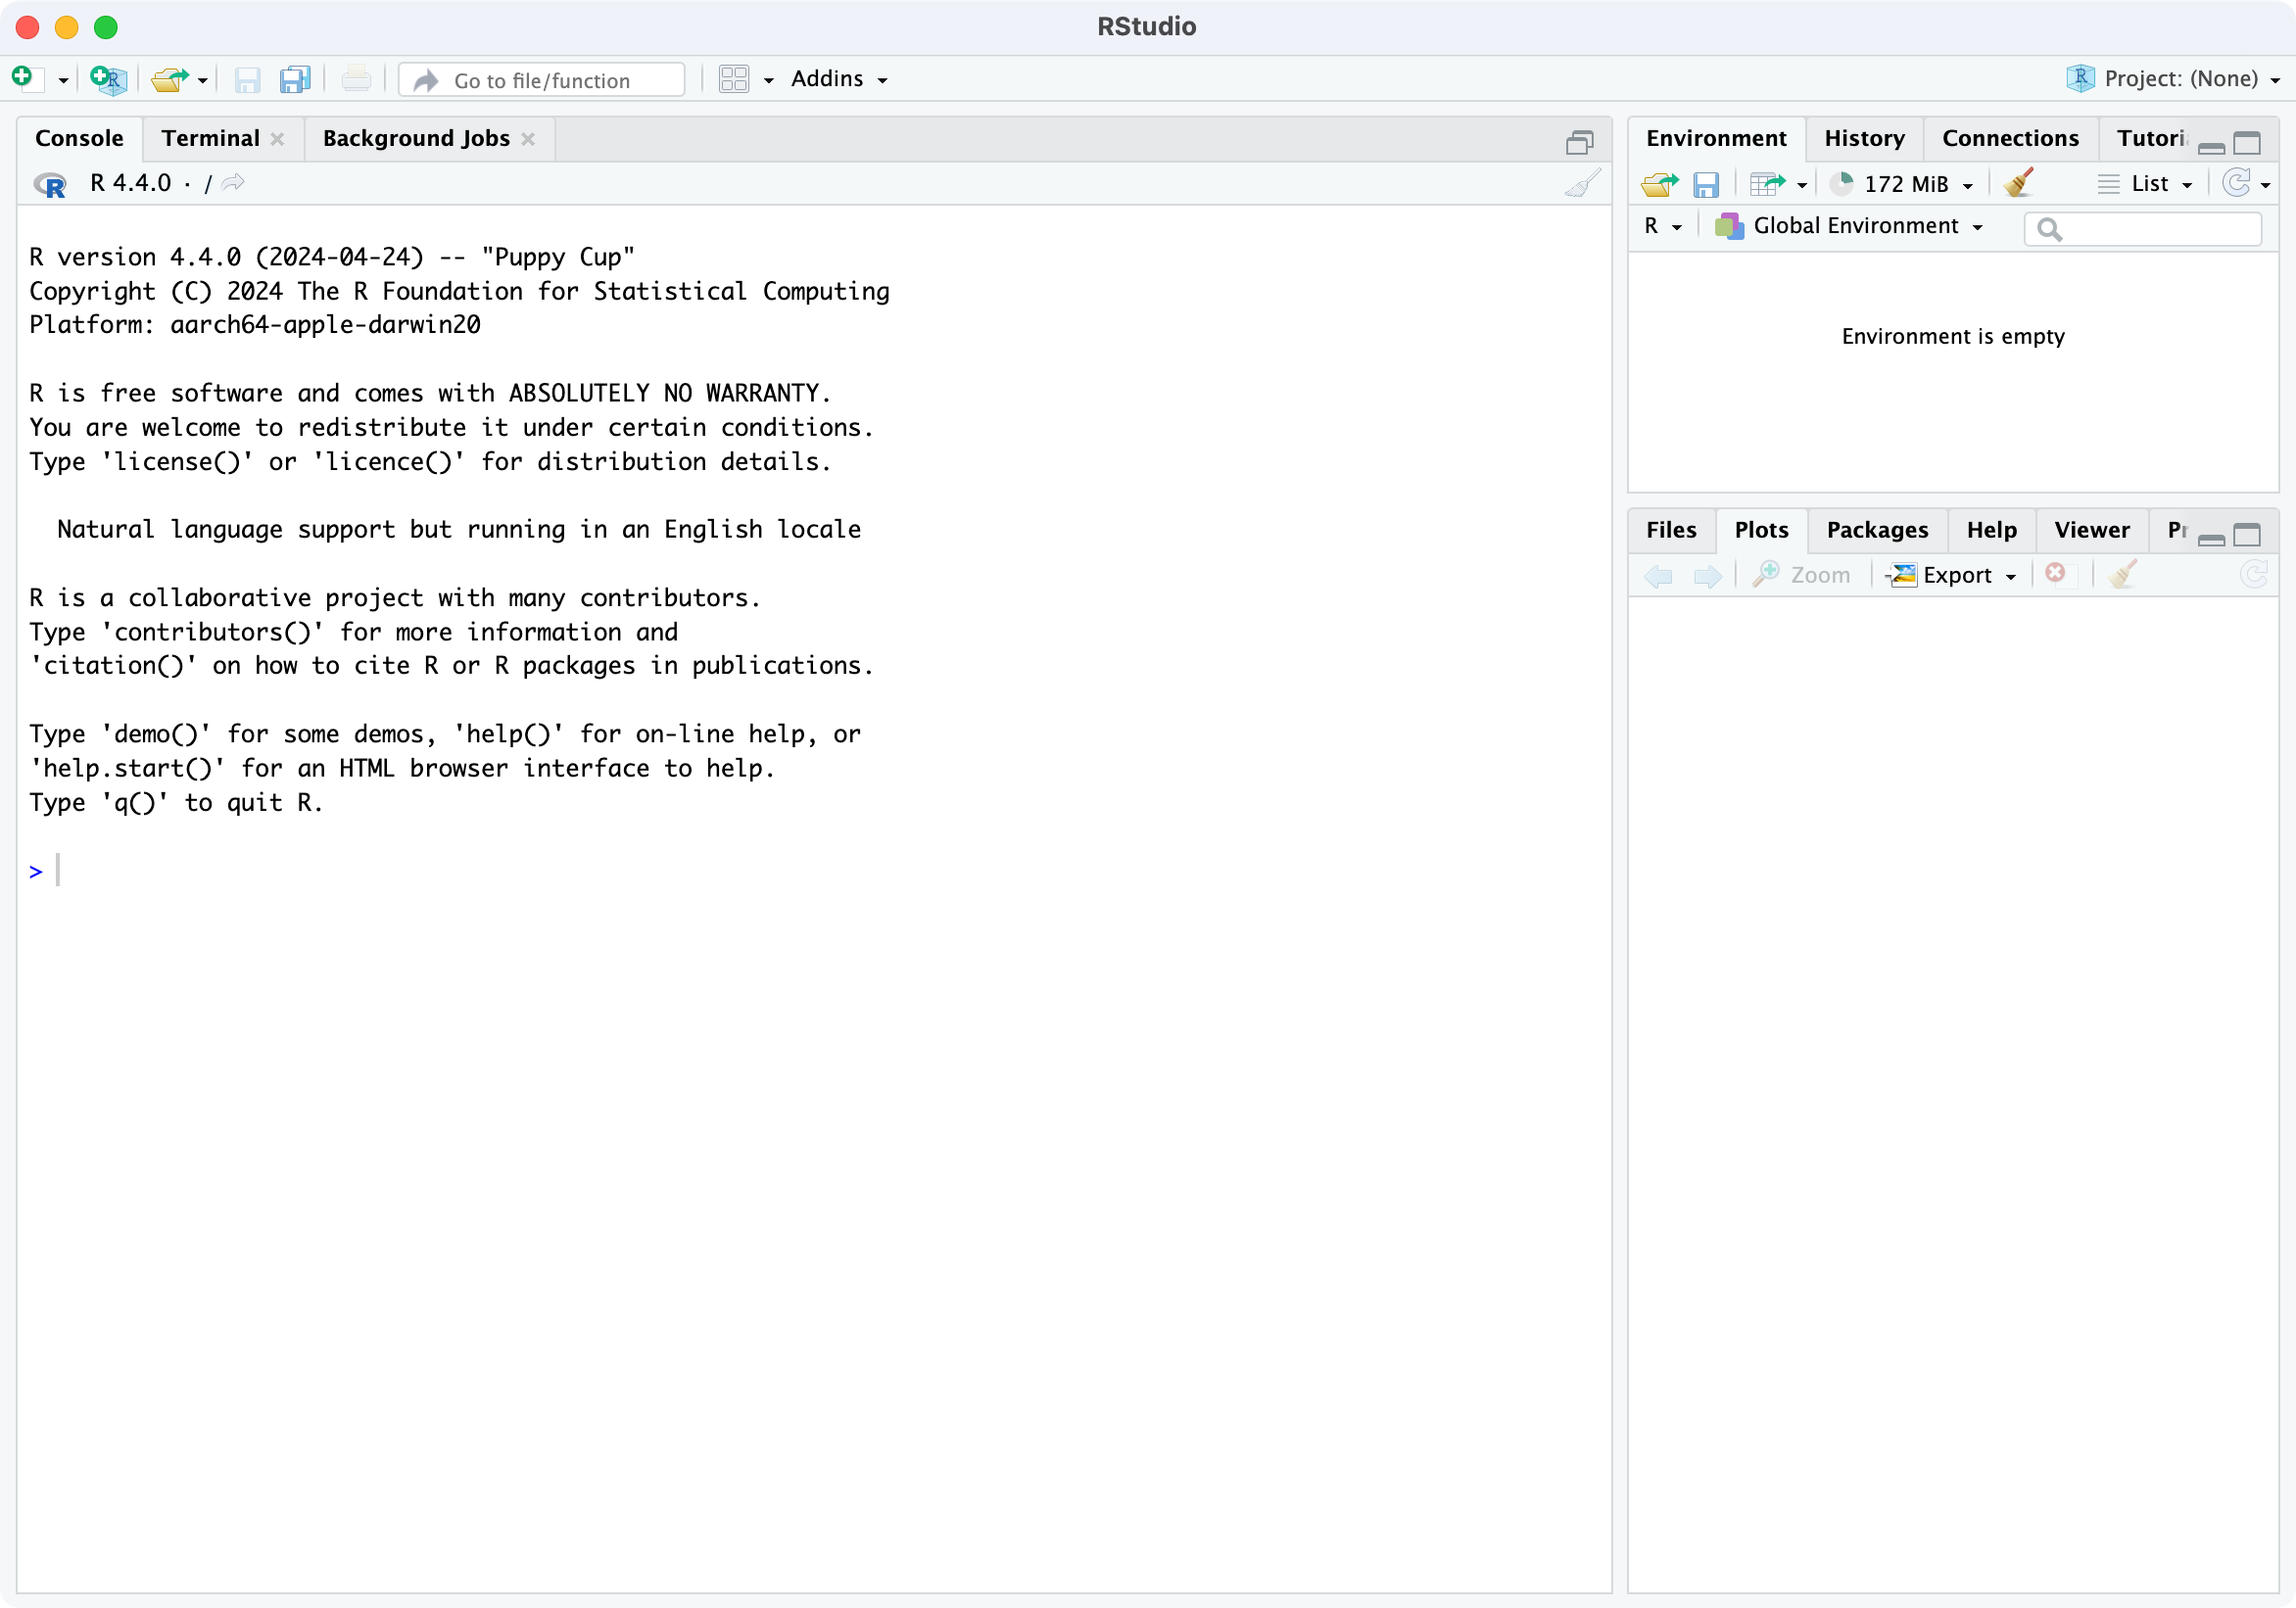
\includegraphics[width=1\linewidth,height=\textheight,keepaspectratio]{img/mod01/RStudio-screenshot-01.png}

Locate the R's command line symbol ``\textgreater{}'' at the bottom of
the left-hand panel. Type \texttt{1\ +\ 2} into the command line and hit
enter, and you will see:

\texttt{{[}1{]}\ 3}

This confirms that RStudio is running correctly, and can use the R
language to correctly calculate the sum between 1 and 2!

RStudio currently comprises three window panes, and we will discuss
these later.

\begin{tcolorbox}[enhanced jigsaw, arc=.35mm, bottomrule=.15mm, bottomtitle=1mm, breakable, colback=white, colbacktitle=quarto-callout-note-color!10!white, colframe=quarto-callout-note-color-frame, coltitle=black, left=2mm, leftrule=.75mm, opacityback=0, opacitybacktitle=0.6, rightrule=.15mm, title={TASK}, titlerule=0mm, toprule=.15mm, toptitle=1mm]

Install R and RStudio and confirm they are both working correctly.

\end{tcolorbox}

\subsection{Recommended setup}\label{recommended-setup}

I will provide a recommended setup for R and RStudio in this section.
You are free to use alternative workflows and setup, but this setup
works well in practice.

\subsubsection{RStudio preferences}\label{rstudio-preferences}

By default, RStudio will retain data, scripts and other objects when you
quit your RStudio session. Relying on this can cause headaches, so I
recommend that you set up RStudio so that it does not preserve your
workspace between sessions. Open the RStudio options:

\begin{itemize}
\item
  Mac: \textbf{Edit \textgreater{} Settings}
\item
  Windows: \textbf{Tools \textgreater{} Global Options}
\end{itemize}

Make sure you are in the \textbf{General} pane, and \textbf{untick
``Restore .RData into workplace at startup''}, and choose:
``\textbf{Save workspace to .RData on exit:} \textbf{Never''}.

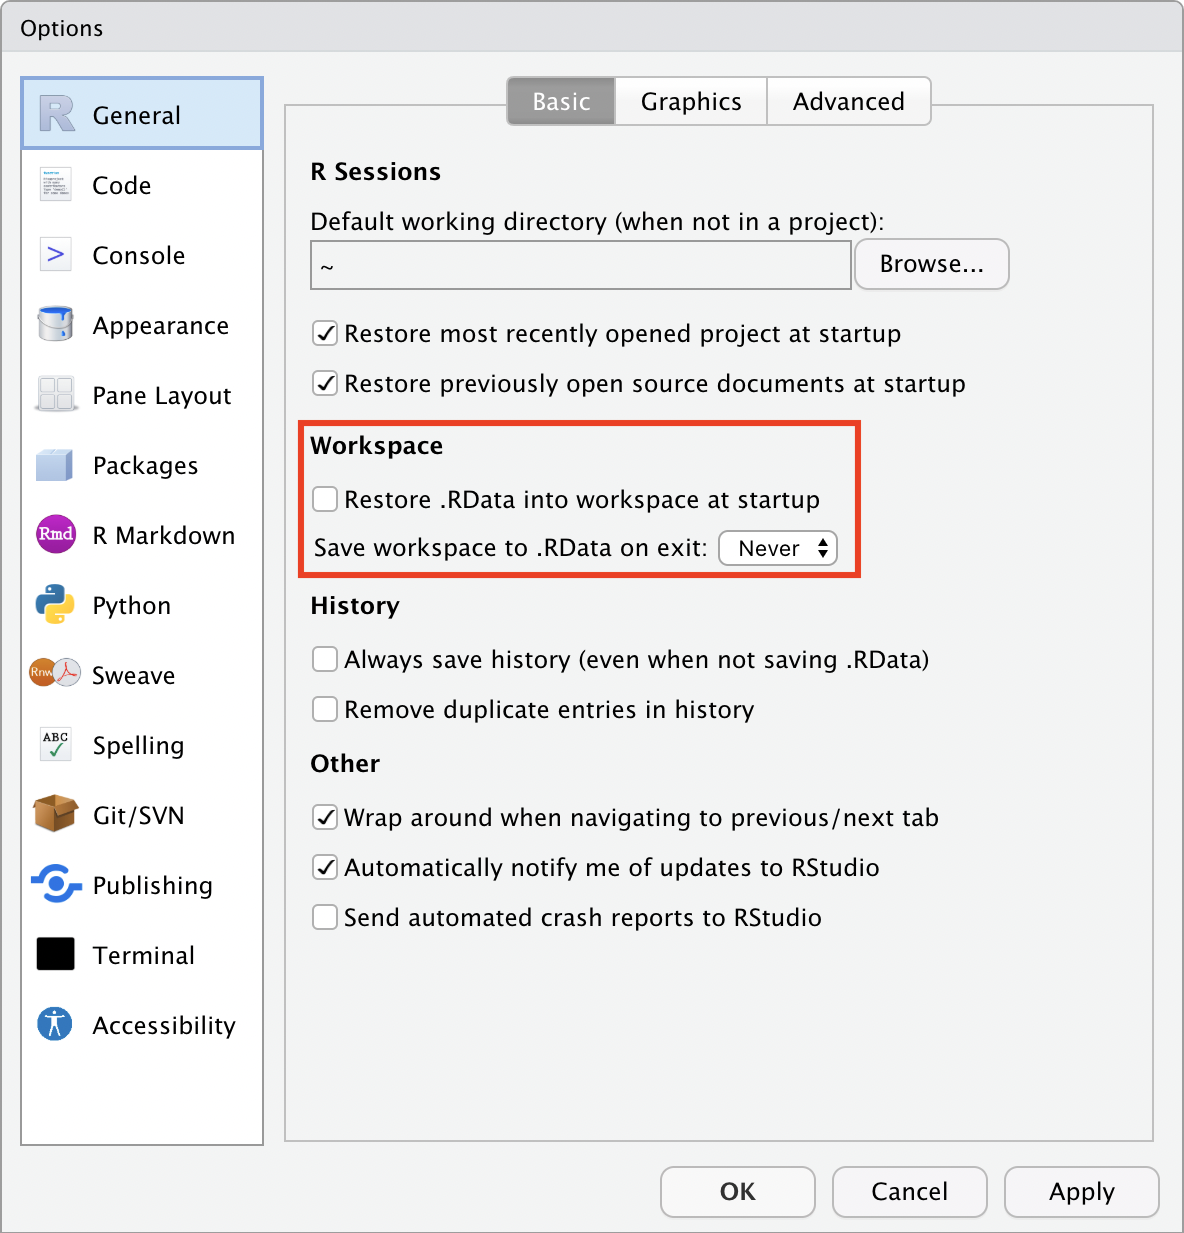
\includegraphics[width=0.75\linewidth,height=\textheight,keepaspectratio]{img/mod01/RStudio-preferences.png}

\subsubsection{Set up a project}\label{set-up-a-project}

A project in RStudio is a folder that RStudio recognises as a place to
store R scripts, data files, figures that are common to an analysis
project. Setting up a folder allows much more simple navigation and
specification of data files and output. More detail can be found in
Chapter 8 of the excellent text:
\href{https://r4ds.had.co.nz/workflow-projects.html}{R for Data
Science}. Using projects is not necessary, but I recommend working with
projects from day one.

We will create a project called \textbf{PHCM9795} to store all the data
you will use and scripts that you will write in this course. First,
think about where you want to store your project folder: this could be
somewhere in your \emph{Documents} folder.

Step 1: Choose \textbf{File \textgreater{} New Project\ldots{}} in
RStudio to open the \textbf{Create Project} dialog box. Click the first
option to create a project in a \textbf{New directory}:

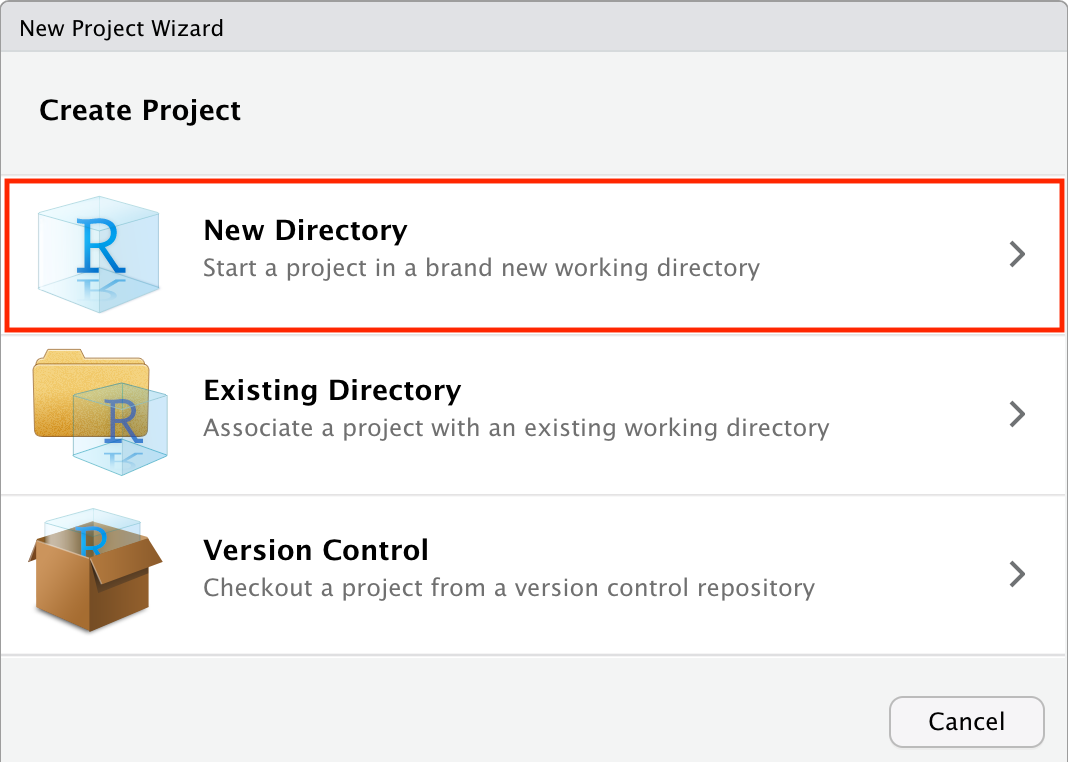
\includegraphics[width=0.75\linewidth,height=\textheight,keepaspectratio]{img/mod01/NewProject-1.png}

Step 2: Click the first option: \textbf{New Project}:

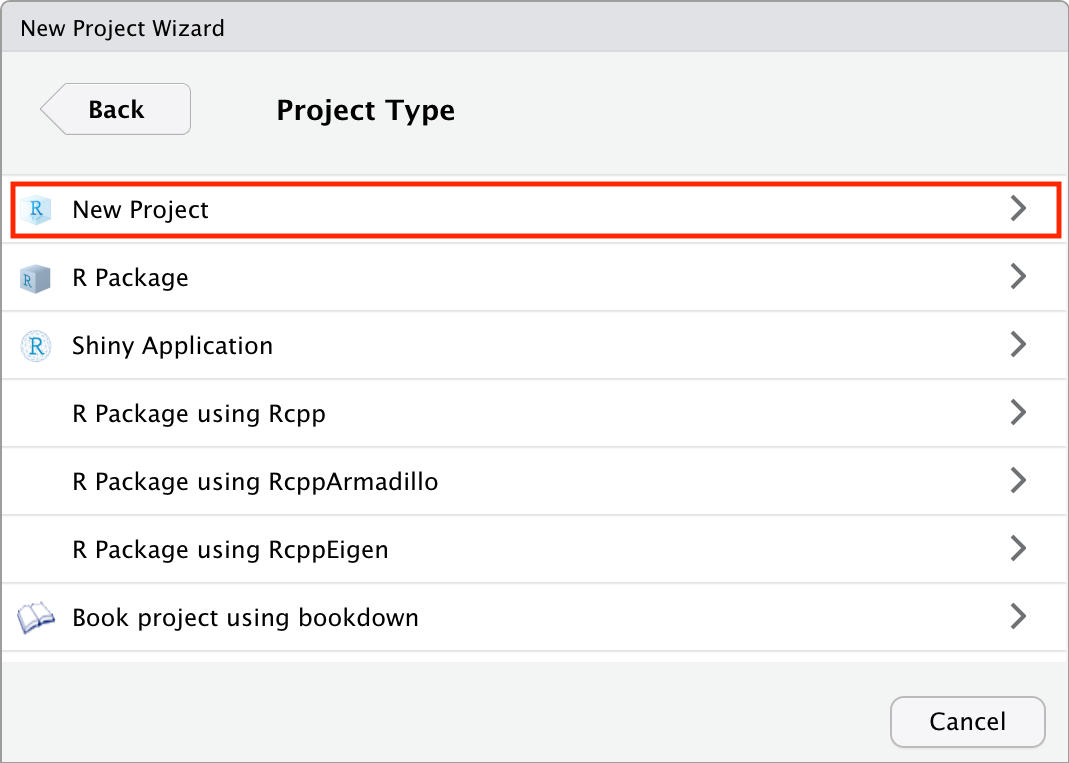
\includegraphics[width=0.75\linewidth,height=\textheight,keepaspectratio]{img/mod01/NewProject-2.png}

Step 3: Give the project a name, by typing PHCM9795 in the ``Directory
name'', and choose where you want to store the project by clicking the
\textbf{Browse} button. Finally, click \textbf{Create} to create your
project.

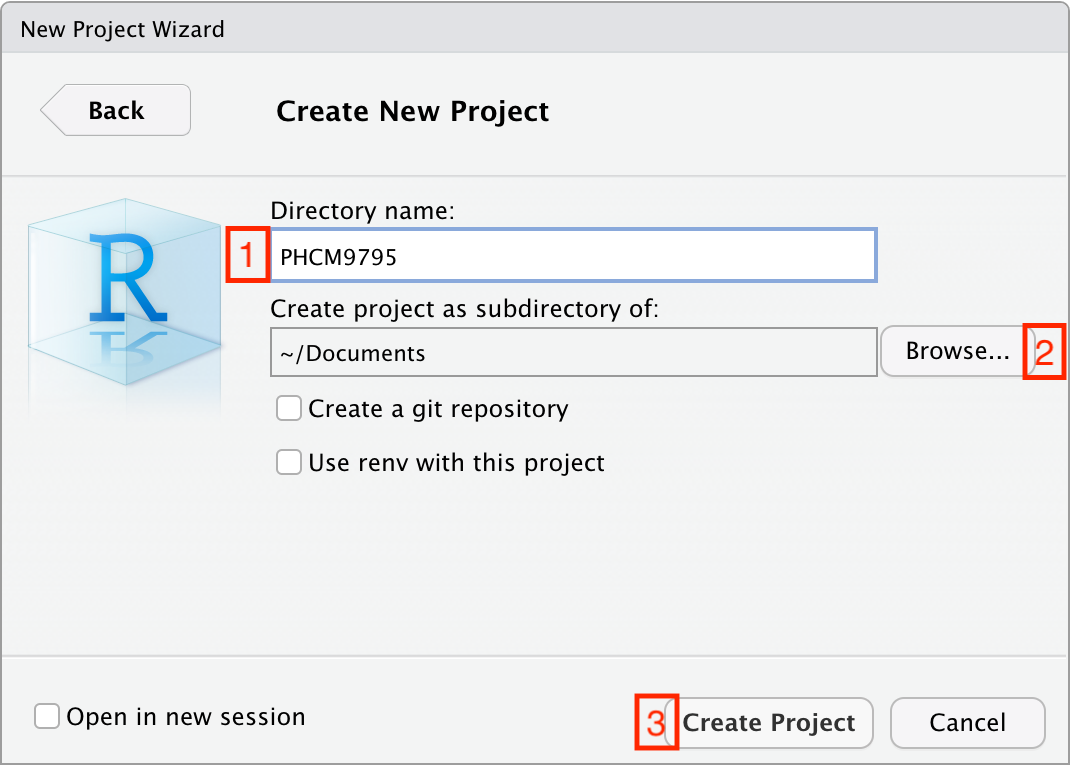
\includegraphics[width=0.75\linewidth,height=\textheight,keepaspectratio]{img/mod01/NewProject-3.png}

You will now have a new folder in your directory, which contains only
one file: PHCM9795.Rproj, and the two right-hand panes of RStudio will
appear as below:

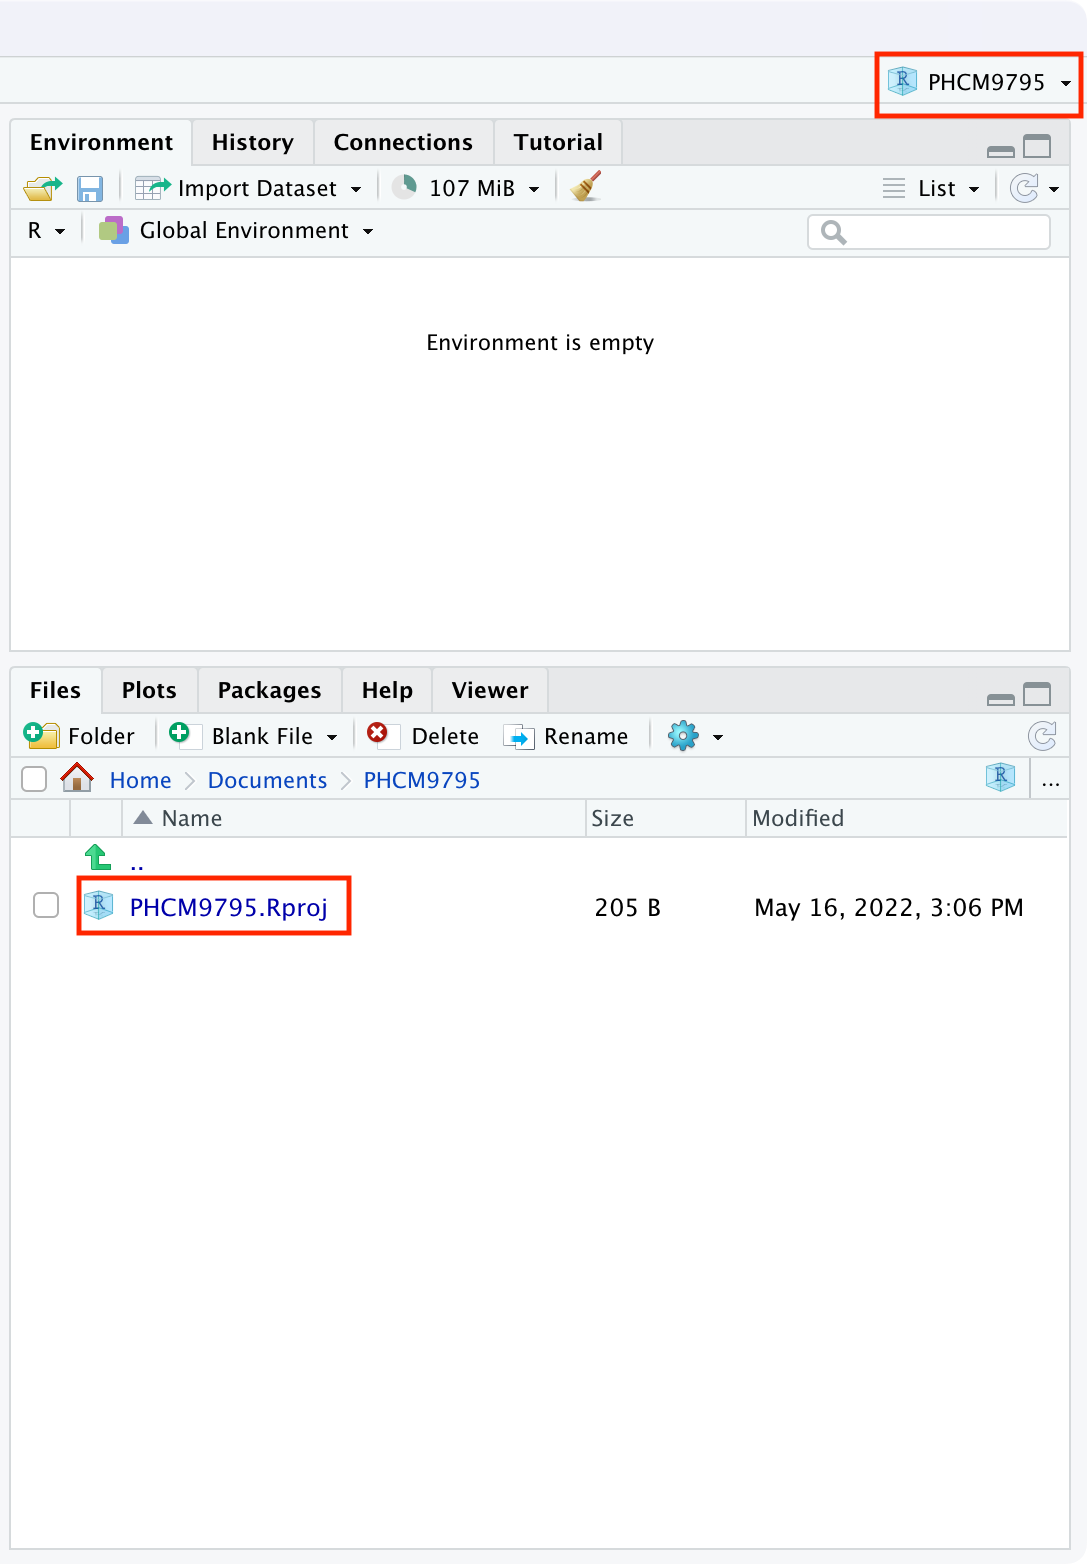
\includegraphics[width=0.75\linewidth,height=\textheight,keepaspectratio]{img/mod01/NewProject-4.png}

\begin{tcolorbox}[enhanced jigsaw, arc=.35mm, bottomrule=.15mm, bottomtitle=1mm, breakable, colback=white, colbacktitle=quarto-callout-note-color!10!white, colframe=quarto-callout-note-color-frame, coltitle=black, left=2mm, leftrule=.75mm, opacityback=0, opacitybacktitle=0.6, rightrule=.15mm, title={TASK}, titlerule=0mm, toprule=.15mm, toptitle=1mm]

Create a new project called PHCM9795. Store it in a folder that you will
remember, so that you can store all your R work in the same folder over
the term.

\end{tcolorbox}

The top-right menu bar is showing that you are working within the
PHCM9795 project, and the bottom-right window is showing the contents of
that window: the single PHCM9795.Rproj file. We will add some more files
to this project later.

\subsection{A simple R analysis}\label{sec-simpleR}

In this very brief section, we will introduce R by calculating the
average of six ages.

To begin, open a new R Script by choosing \textbf{File \textgreater{}
New file \textgreater{} R Script} . A script (or a program) is a
collection of commands that are sequentially processed by R. You can
also type Ctrl+Shift+N in Windows, or Command+Shift+N in MacOS to open a
new script in RStudio, or click the \textbf{New File} button at the top
of the RStudio window.

You should now see four window panes, as below. In the top-left window,
type the following (replacing my name with yours, and including today's
date):

\begin{Shaded}
\begin{Highlighting}[]
\CommentTok{\# Author: Timothy Dobbins}
\CommentTok{\# Date: 5 April 2024}
\CommentTok{\# Purpose: My first R script}

\NormalTok{age }\OtherTok{\textless{}{-}} \FunctionTok{c}\NormalTok{(}\DecValTok{20}\NormalTok{, }\DecValTok{25}\NormalTok{, }\DecValTok{23}\NormalTok{, }\DecValTok{29}\NormalTok{, }\DecValTok{21}\NormalTok{, }\DecValTok{27}\NormalTok{)}
\FunctionTok{summary}\NormalTok{(age)}
\end{Highlighting}
\end{Shaded}

\textbf{Note: R is case-sensitive}, so you should enter the text exactly
as written in these notes.

Your screen should look like:

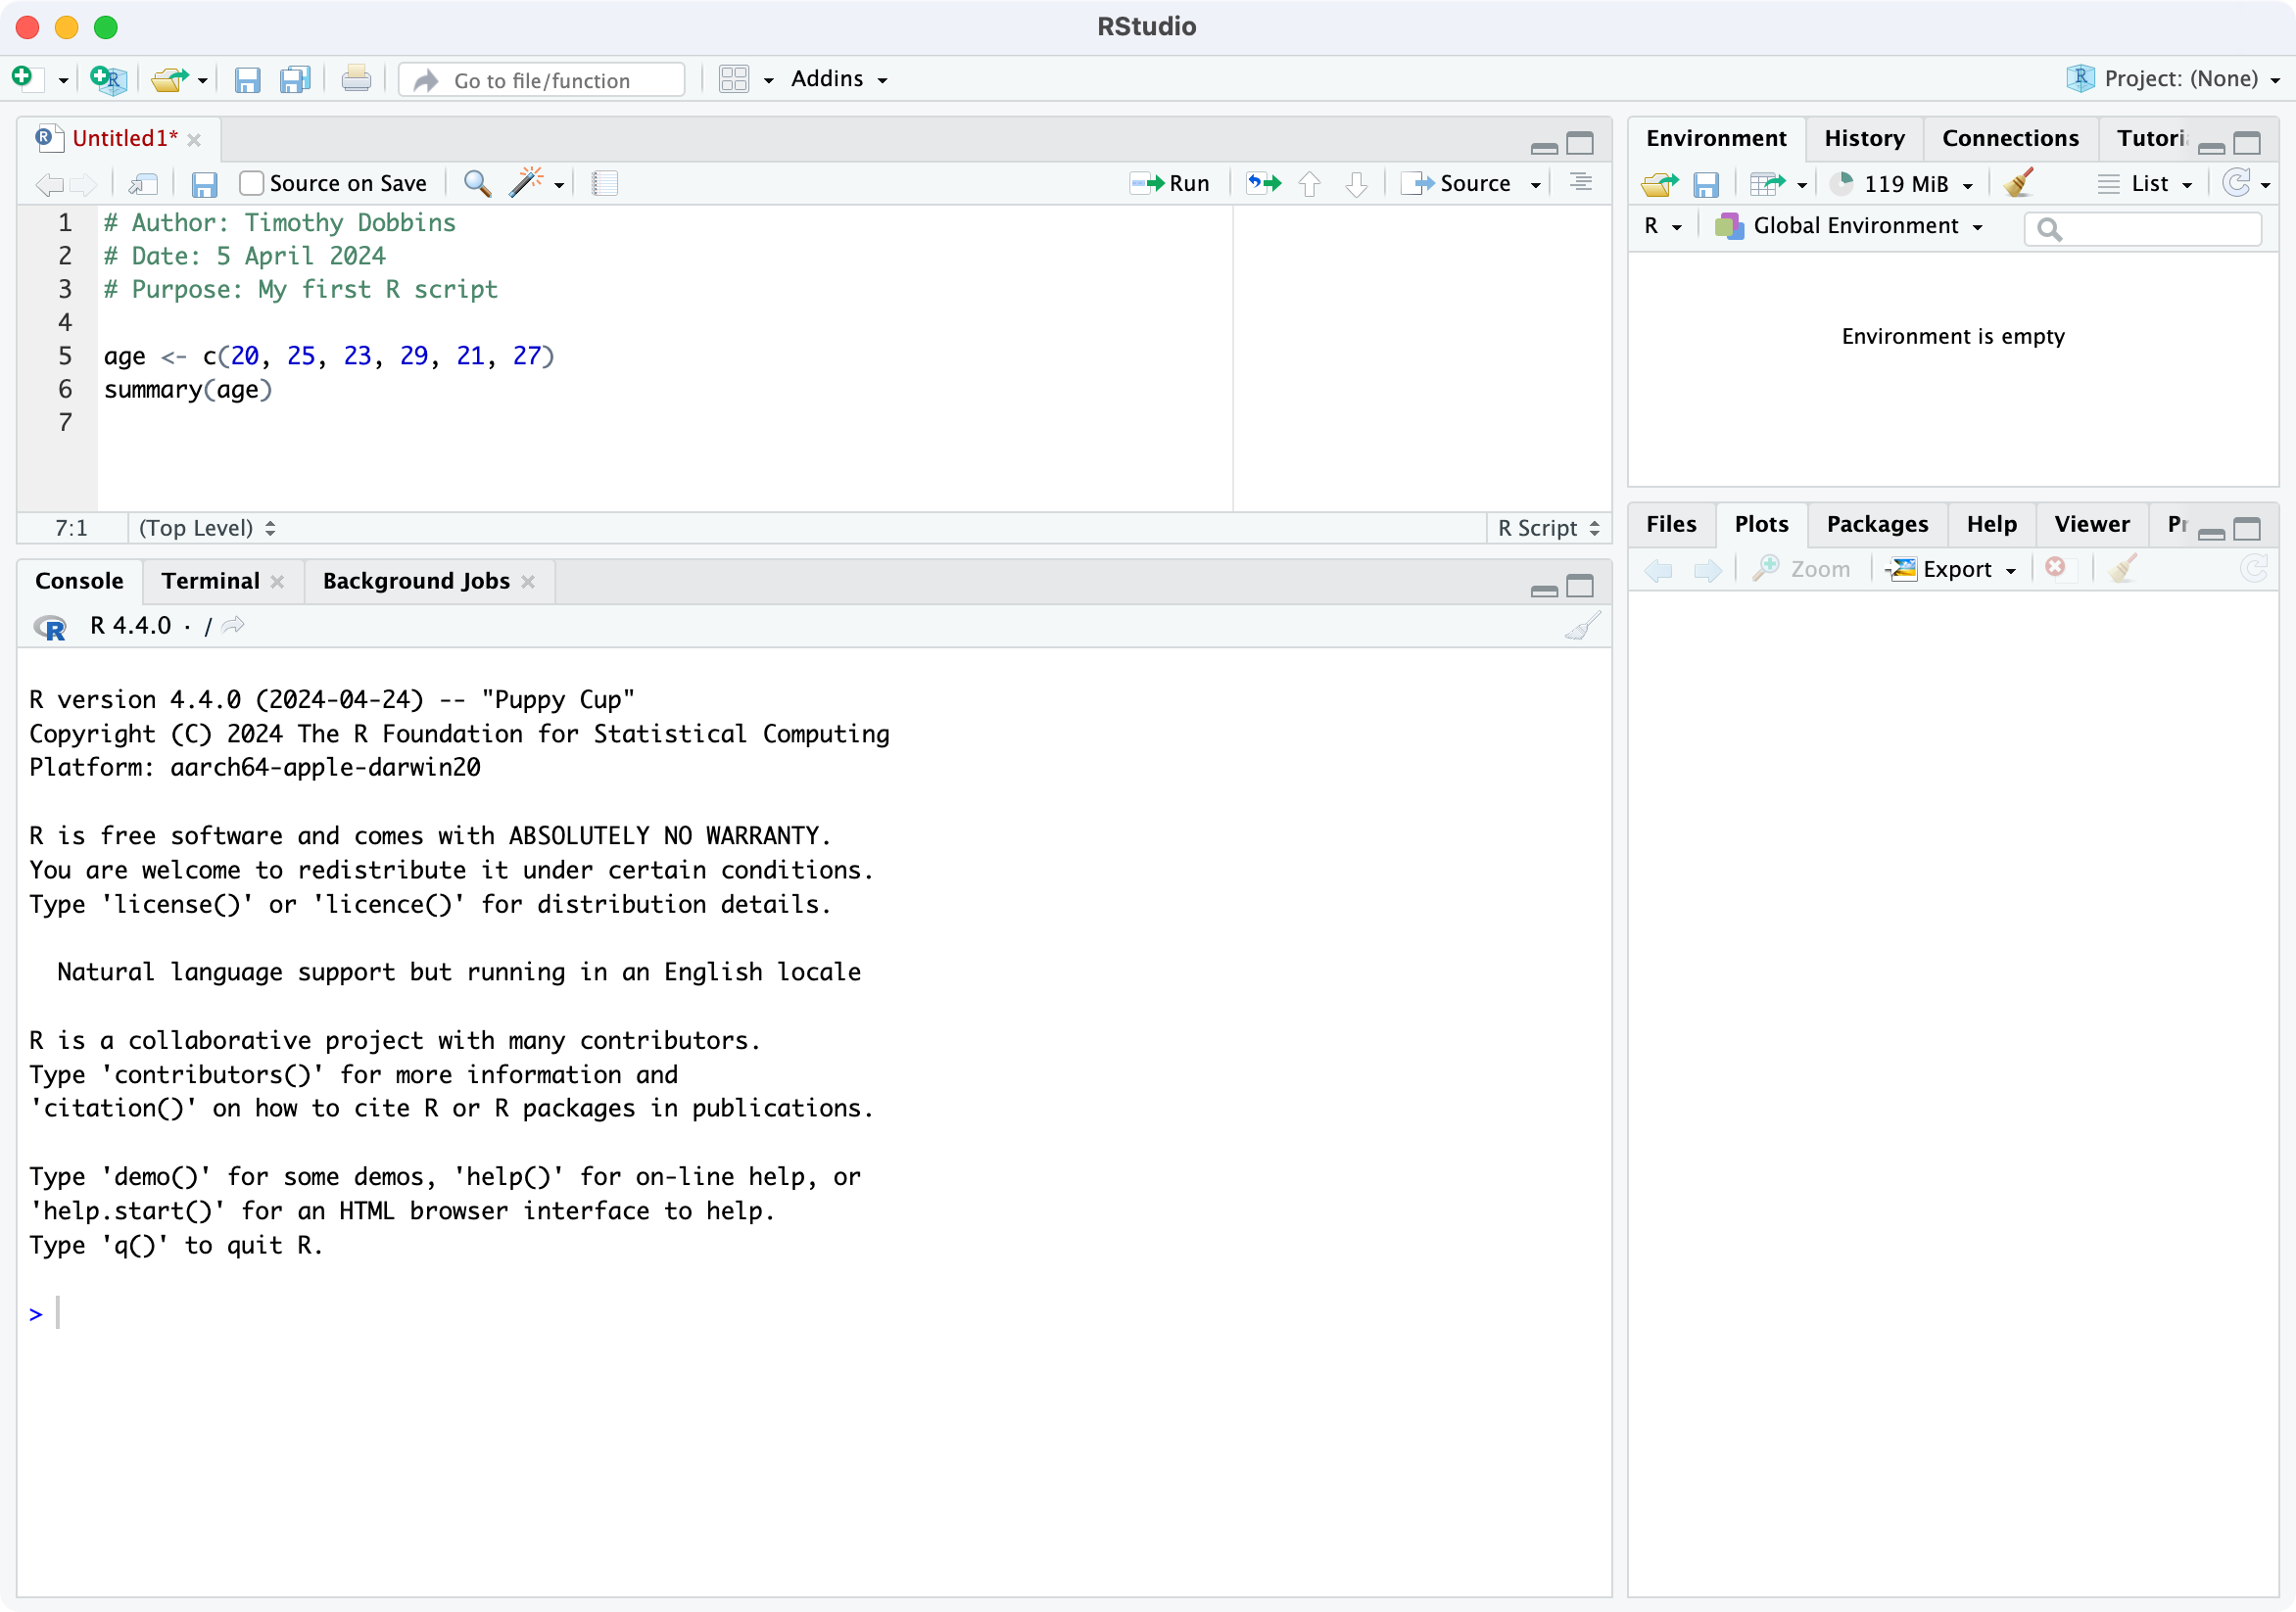
\includegraphics[width=1\linewidth,height=\textheight,keepaspectratio]{img/mod01/RStudio-screenshot-02.png}

To run your script, choose \textbf{Code \textgreater{} Run Region
\textgreater{} Run All} from the menu bar. You will see your code appear
in the bottom-left window, with the following output:

\begin{Shaded}
\begin{Highlighting}[]
\SpecialCharTok{\textgreater{}} \CommentTok{\# Author: Timothy Dobbins}
\ErrorTok{\textgreater{}} \CommentTok{\# Date: 5 April 2024}
\ErrorTok{\textgreater{}} \CommentTok{\# Purpose: My first R script}
\ErrorTok{\textgreater{}}
\ErrorTok{\textgreater{}}\NormalTok{ age }\OtherTok{\textless{}{-}} \FunctionTok{c}\NormalTok{(}\DecValTok{20}\NormalTok{, }\DecValTok{25}\NormalTok{, }\DecValTok{23}\NormalTok{, }\DecValTok{29}\NormalTok{, }\DecValTok{21}\NormalTok{, }\DecValTok{27}\NormalTok{)}

\SpecialCharTok{\textgreater{}} \FunctionTok{summary}\NormalTok{(age)}
\NormalTok{   Min. }\DecValTok{1}\NormalTok{st Qu.  Median    Mean }\DecValTok{3}\NormalTok{rd Qu.    Max.}
  \FloatTok{20.00}   \FloatTok{21.50}   \FloatTok{24.00}   \FloatTok{24.17}   \FloatTok{26.50}   \FloatTok{29.00}
\end{Highlighting}
\end{Shaded}

We will explain the key parts of this script later, but for now, you
have entered six ages and calculated the mean age (along with five other
summary statistics).

\begin{tcolorbox}[enhanced jigsaw, arc=.35mm, bottomrule=.15mm, bottomtitle=1mm, breakable, colback=white, colbacktitle=quarto-callout-note-color!10!white, colframe=quarto-callout-note-color-frame, coltitle=black, left=2mm, leftrule=.75mm, opacityback=0, opacitybacktitle=0.6, rightrule=.15mm, title={TASK}, titlerule=0mm, toprule=.15mm, toptitle=1mm]

Type the code above into the top-left window, and run the script.

Save your script within the PHCM9795 project by using \textbf{File
\textgreater{} Save As}, using the name \texttt{my\_first\_analysis.R}.

\end{tcolorbox}

\subsection{The RStudio environment}\label{the-rstudio-environment}

Now that we have seen a simple example of how to use R within RStudio,
let's describe the RStudio environment. Let's assume that you have just
run your first R script, and you have four windows as below:

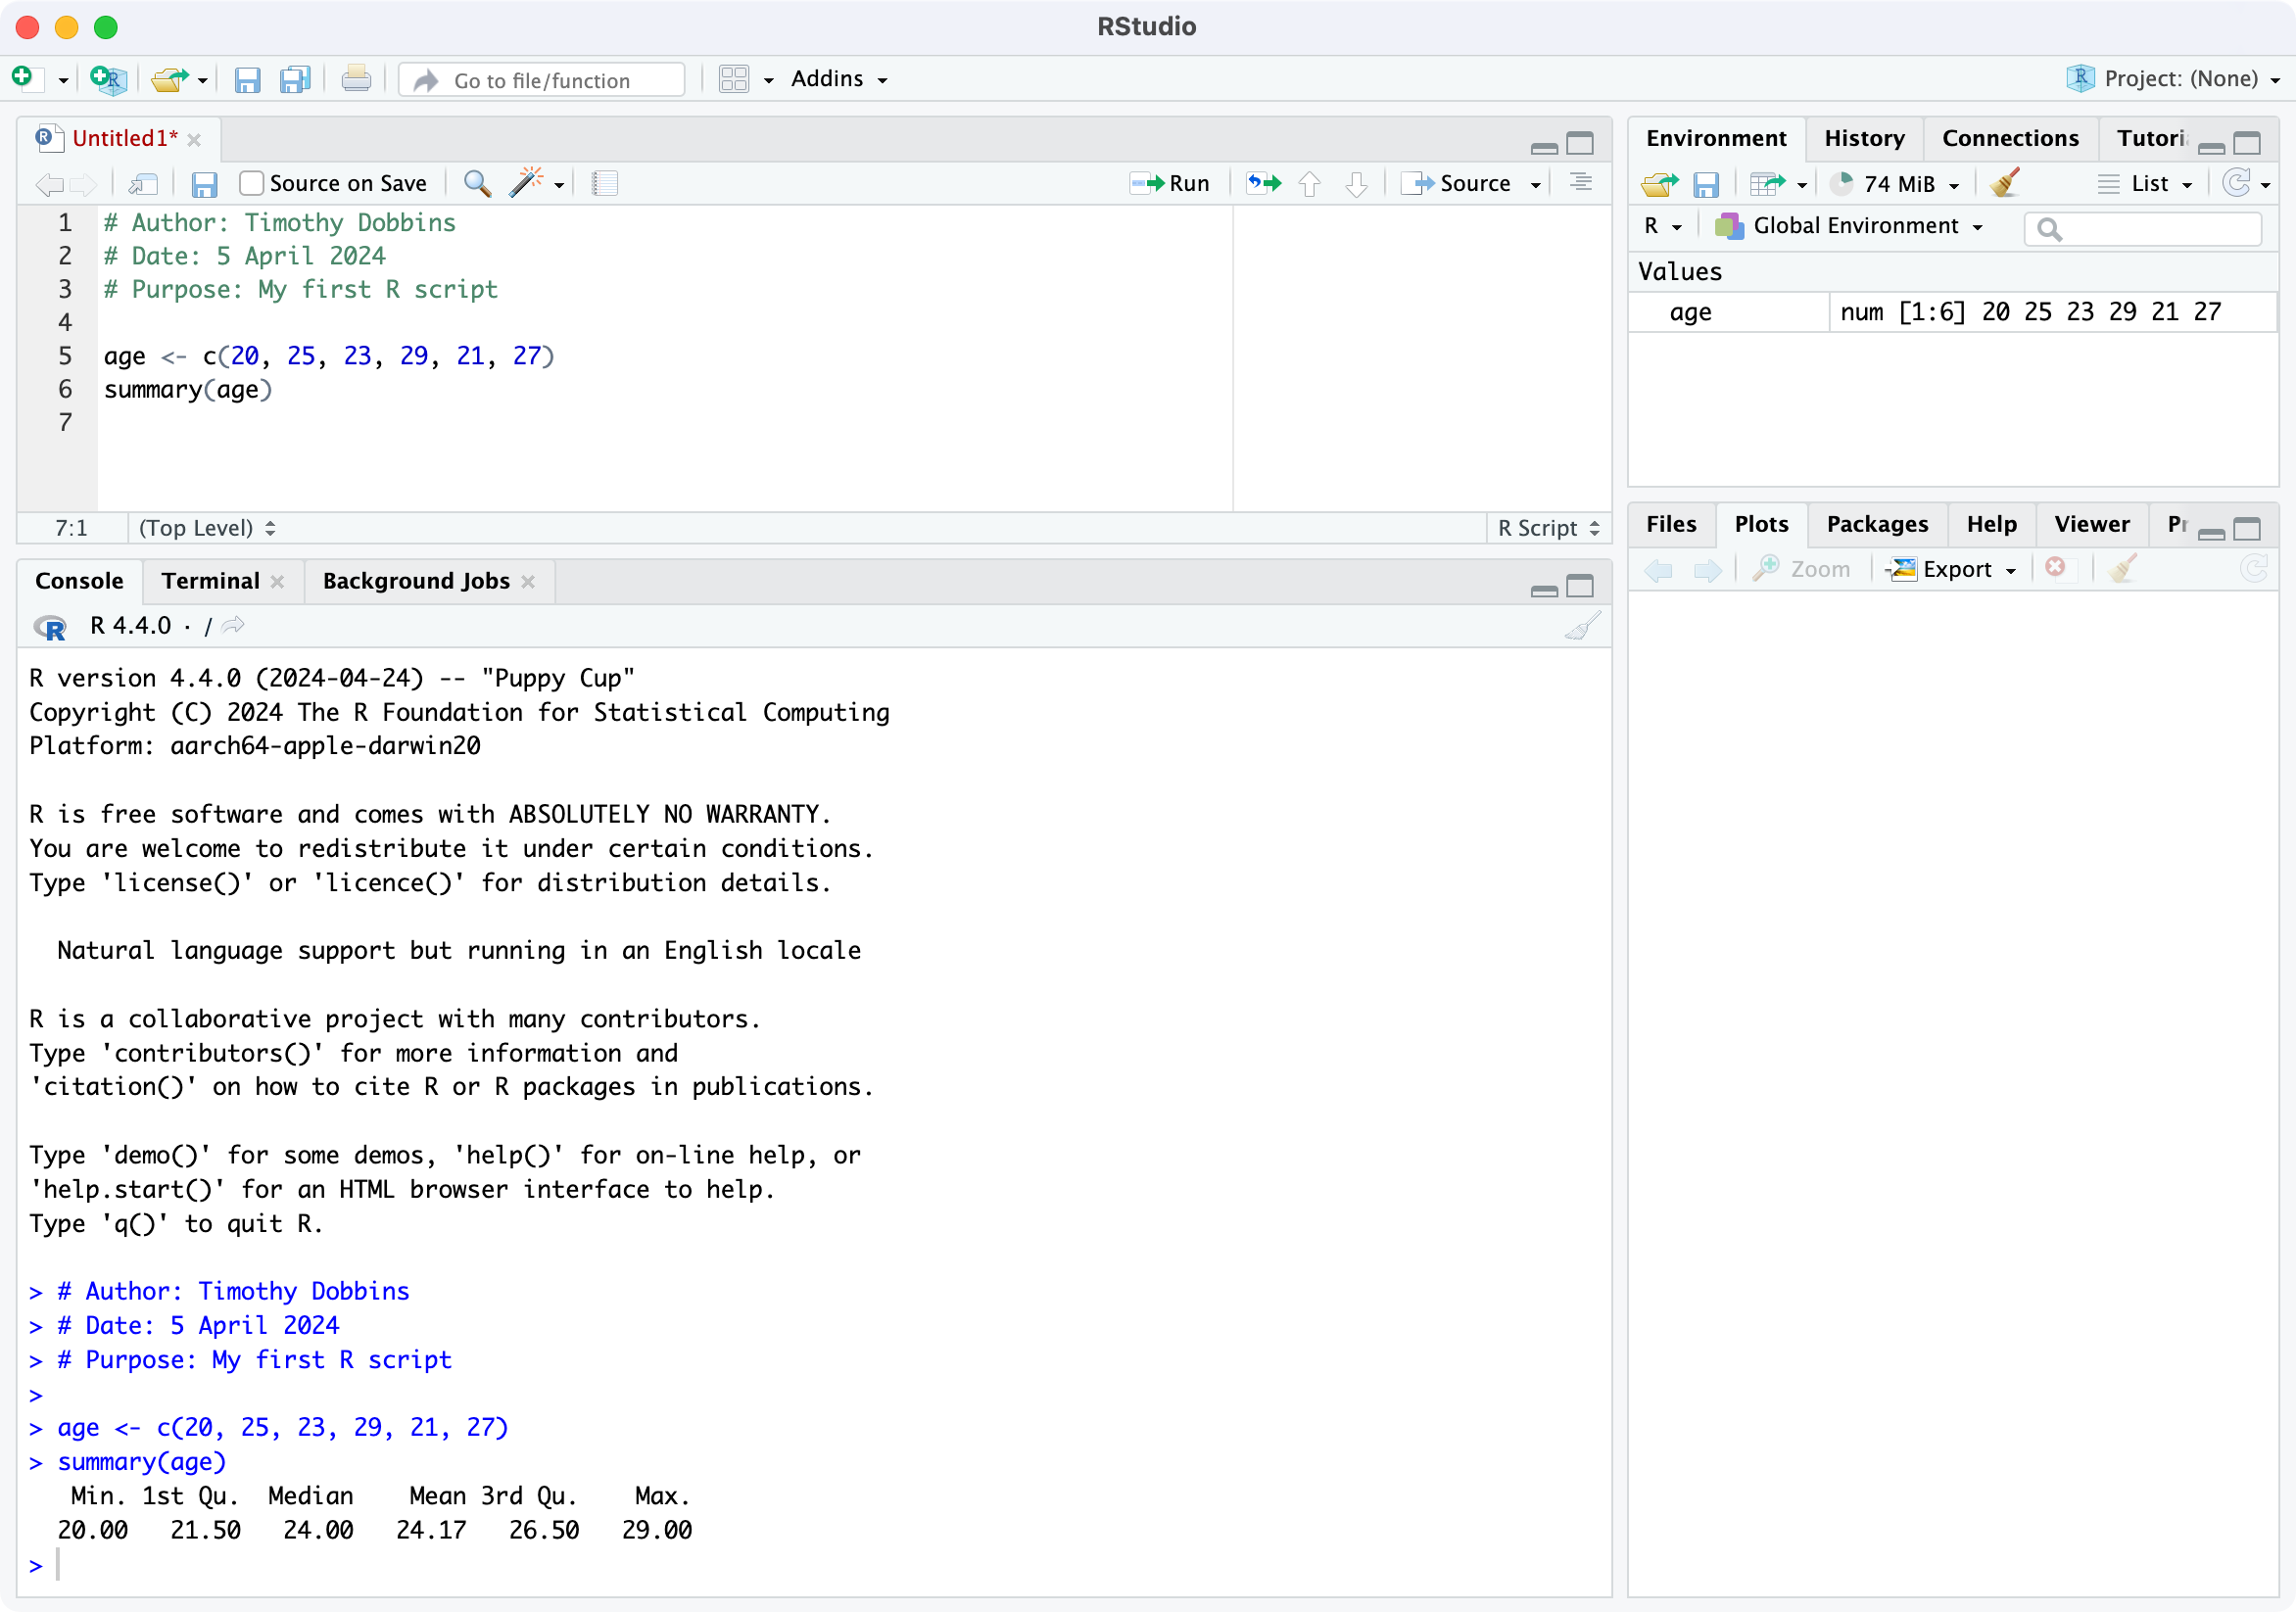
\includegraphics[width=1\linewidth,height=\textheight,keepaspectratio]{img/mod01/RStudio-screenshot-03.png}

The top-left window is call the \textbf{Source} window, and is where you
write and edit your R scripts. Scripts can be saved by clicking
\textbf{File \textgreater{} Save As} or by clicking on the symbol of a
floppy disk at the top of the script. The file will have an extension of
.R, for example script.R. Remember to give your script a meaningful
title and remember to periodically save as you go.

Notice the tab at the top of the Source window which includes the name
of the current file. The name of the script will be black when it has
been saved, and will change to red if you have any unsaved changes.

The \textbf{Console} window, at the bottom left, contains the command
line which is indicated with the symbol \textgreater. You can type
commands here, but anything executed directly from the console is not
saved and therefore is lost when the session ends (when you exit
RStudio). You should always run your commands from a script file which
you can save and use again later. When you run commands from a script,
the output and any notes/errors are shown in the console. The Terminal
and Jobs tabs will not be used in this course.

The \textbf{Environment} window at the top-right shows a list of objects
that have been created during your session. When you close your RStudio
session these objects will disappear. We will not use the History or
Connections tabs in this course.

The bottom right corner contains some useful tabs, in particular the
\textbf{Help} tab. When you are troubleshooting errors or learning how
to use a function, the Help tab should be the first place you visit.
Here you can search the help documents for all the packages you have
installed. Whenever you create plots in R, these will be shown in the
\textbf{Plots} tab. The \textbf{Packages} tab contains a list of
installed packages and indicates which ones are currently in use (we
will learn about packages later). Packages which are loaded, i.e.~in
use, are indicated with a tick. Some packages are in use by default when
you begin a new session. You can access information about a package by
clicking on its name. The \textbf{Files} tab provides a shortcut to
access your files. The Viewer tab will not be used in this course.

\subsection{Some R basics}\label{some-r-basics}

While we use R as a statistics package, R is a programming language. In
order to use R effectively, we need to define some basics.

\subsubsection{Scripts}\label{scripts}

While R can be run completely from the command line, issuing commands
one-by-one, it is most commonly run using \textbf{scripts}. A script is
simply a list of commands that are processed in order. The simple
analysis we conducted earlier is a very simple script. Some things to
know about R scripts:

\begin{itemize}
\item
  anything appearing after a \# is a comment, and is ignored by R. The
  first three lines of our script are there for ourselves (either as
  writers of code, or readers of code). I include comments at the
  beginning of each of my scripts to describe:

  \begin{itemize}
  \item
    who wrote the script (useful if someone else uses your script and
    wants to ask questions about it);
  \item
    when the script was written;
  \item
    what the script does. This last point may seem odd, but it's useful
    to describe what this script does, and why it might differ to other
    scripts being used in the analysis. This is particularly useful if
    your scripts become long and complex.
  \end{itemize}
\item
  \textbf{R is case-sensitive}. So \texttt{age}, \texttt{AGE} and
  \texttt{Age} could refer to three separate variables (please don't do
  this!)
\item
  use blank lines and comments to separate sections of your script
\end{itemize}

\subsubsection{Objects}\label{objects}

If you do some reading about R, you may learn that R is based on
\textbf{objects} and \textbf{functions}. We can think of objects as the
`nouns' of R, and functions as the `verbs'. When we enter data, or
import data into R, we are asking R to create \textbf{objects} from our
data. These objects can be manipulated and transformed by
\textbf{functions}, to obtain useful insights from our data.

Objects in R are created using the \textbf{assignment operator}. The
most common form of the assignment operator looks like an arrow:
\texttt{\textless{}-} and is typed as the \texttt{\textless{}} and
\texttt{-} symbols. The simplest way of reading \texttt{\textless{}-} is
as the words ``is defined as''. Note that it possible to use
\texttt{-\textgreater{}} and even \texttt{=} as assignment operators,
but their use is less frequent.

We created an object earlier, called \texttt{age}, which comprised six
values. Let's see another example:

\begin{Shaded}
\begin{Highlighting}[]
\NormalTok{x }\OtherTok{\textless{}{-}} \DecValTok{42}
\end{Highlighting}
\end{Shaded}

This command creates a new object called \texttt{x}, which is defined as
the number 42 (or in words, ``\texttt{x} is defined as 42''). Running
this command gives no output in the console, but the new object appears
in the top-right \textbf{Environment} panel. We can view the object in
the console by typing its name:

\begin{Shaded}
\begin{Highlighting}[]
\CommentTok{\# Print the object x}
\NormalTok{x}
\end{Highlighting}
\end{Shaded}

\begin{verbatim}
[1] 42
\end{verbatim}

Now we see the contents of \texttt{x} in the console.

This example is rather trivial, and we rarely assign objects of just one
value.

\subsubsection{Data structures}\label{sec-data-structures}

There are two main structures we will use to work with data in this
course: \textbf{vectors} and \textbf{data frames}. A \textbf{vector} is
a combination of data values, all of the same type. For example, our six
ages that we entered earlier is a vector. You could think of a vector as
a column of data (even though R prints vectors as rows!) And
technically, even an object with only one value is a vector, a vector of
size 1.

The easiest way of creating a vector in R is by using the \texttt{c()}
function, where c stands for `combine'. In our previous Simple Analysis
in R (Section~\ref{sec-simpleR}), we wrote the command:

\begin{Shaded}
\begin{Highlighting}[]
\NormalTok{age }\OtherTok{\textless{}{-}} \FunctionTok{c}\NormalTok{(}\DecValTok{20}\NormalTok{, }\DecValTok{25}\NormalTok{, }\DecValTok{23}\NormalTok{, }\DecValTok{29}\NormalTok{, }\DecValTok{21}\NormalTok{, }\DecValTok{27}\NormalTok{)}
\end{Highlighting}
\end{Shaded}

This command created a new object called \texttt{age}, and
\emph{combined} the six values of age into one vector.

Just as having a vector of size 1 is unusual, having just one column of
data to analyse is also pretty unusual. The other structure we will
describe here is a \textbf{data frame} which is essentially a collection
of vectors, each of the same size. You could think of a data frame as
being like a spreadsheet, with columns representing variables, and rows
representing observations.

There are other structures in R, such as matrices and lists, which we
won't discuss in this course. You may also come across the term
\textbf{tibble}, which is a type of data frame.

\subsubsection{Functions}\label{functions}

As the `verbs' of R, functions transform objects. Functions can
transform your data into summary statistics, graphical summaries or
analysis results. For example, we used the \texttt{summary()} function
to display summary statistics for our six ages.

R functions are specified by their arguments (or inputs). The arguments
that can be supplied for each function can be inspected by examining the
help notes for that function. To obtain help for a function, we can
submit \texttt{help(summary)} (or equivalently \texttt{?summary}) in the
console, or we can use the \textbf{Help} tab in the bottom-right window
of RStudio. For example, the first part of the help notes for
\texttt{summary} appear as:

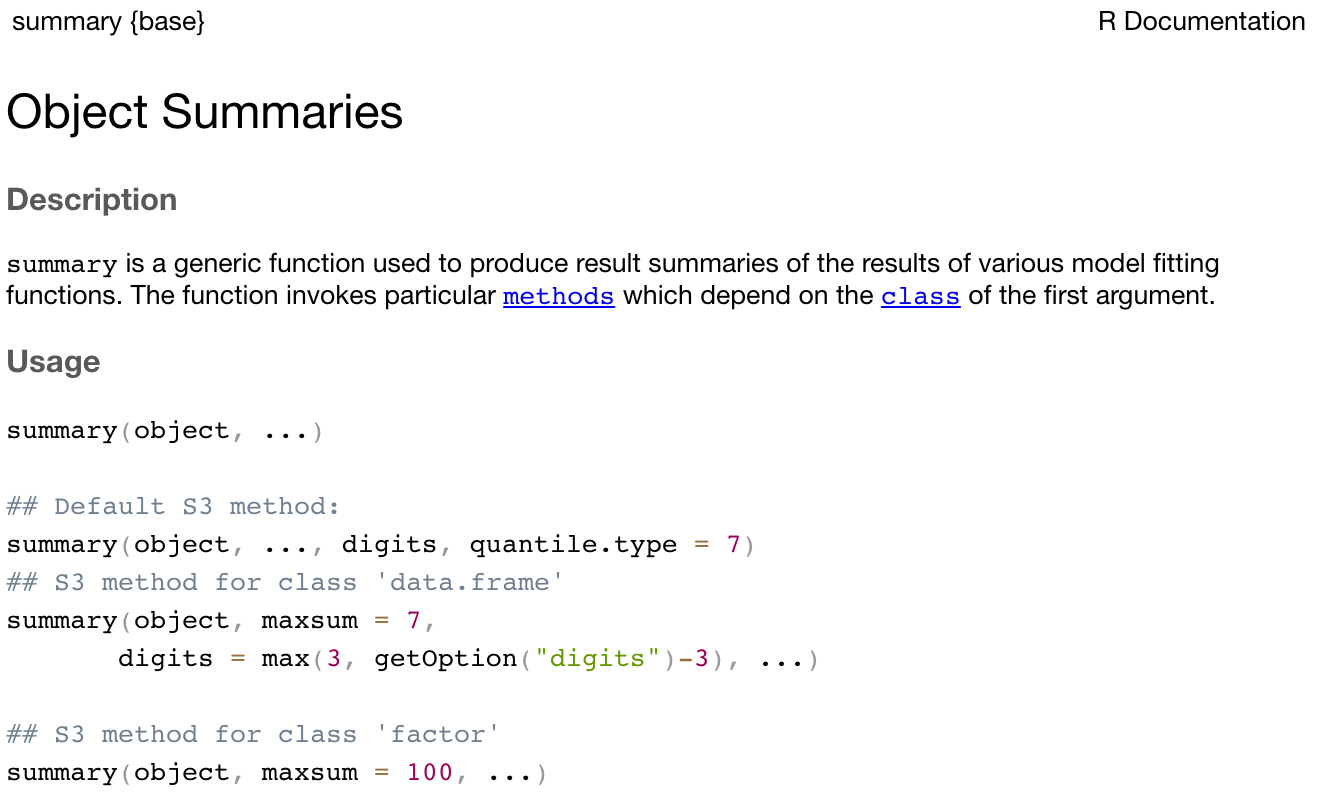
\includegraphics[width=0.8\linewidth,height=\textheight,keepaspectratio]{img/mod01/help-1.png}

The help notes in R can be quite cryptic, but the \textbf{Usage} section
details what inputs should be specified for the function to run. Here,
\texttt{summary} requires an object to be specified. In our case, we
specified \texttt{age}, which is our object defined as the vector of six
ages.

Most help pages also include some examples of how you might use the
function. These can be found at the very bottom of the help page.

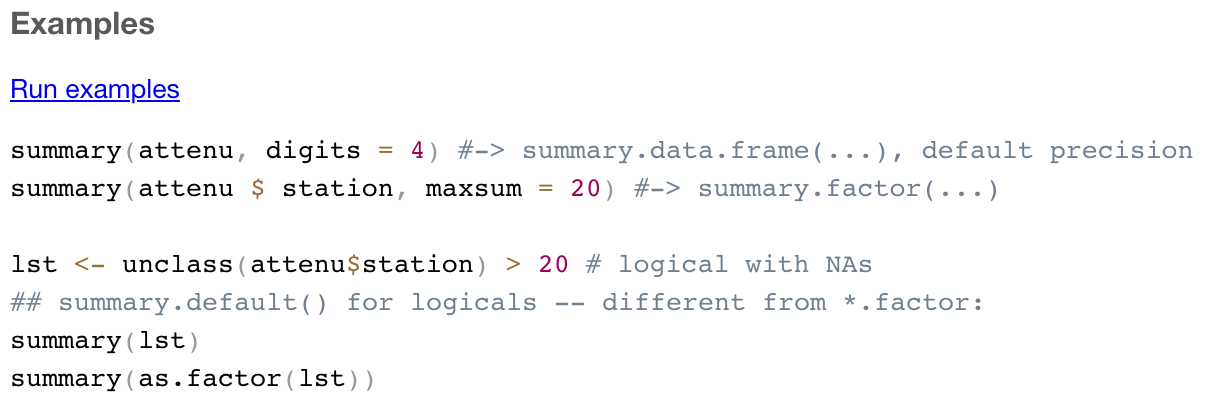
\includegraphics[width=0.8\linewidth,height=\textheight,keepaspectratio]{img/mod01/help-2.png}

The \texttt{summary()} function is quite simple, in that it only
requires one input, the object to be summarised. More complex functions
might require a number of inputs. For example, the help notes for the
\texttt{descriptives()} function in the \texttt{jmv} package show a
large number of inputs can be specified. Instructions for installing the
\texttt{jmv} package will be provided later, this help-screen is
included for illustration only.

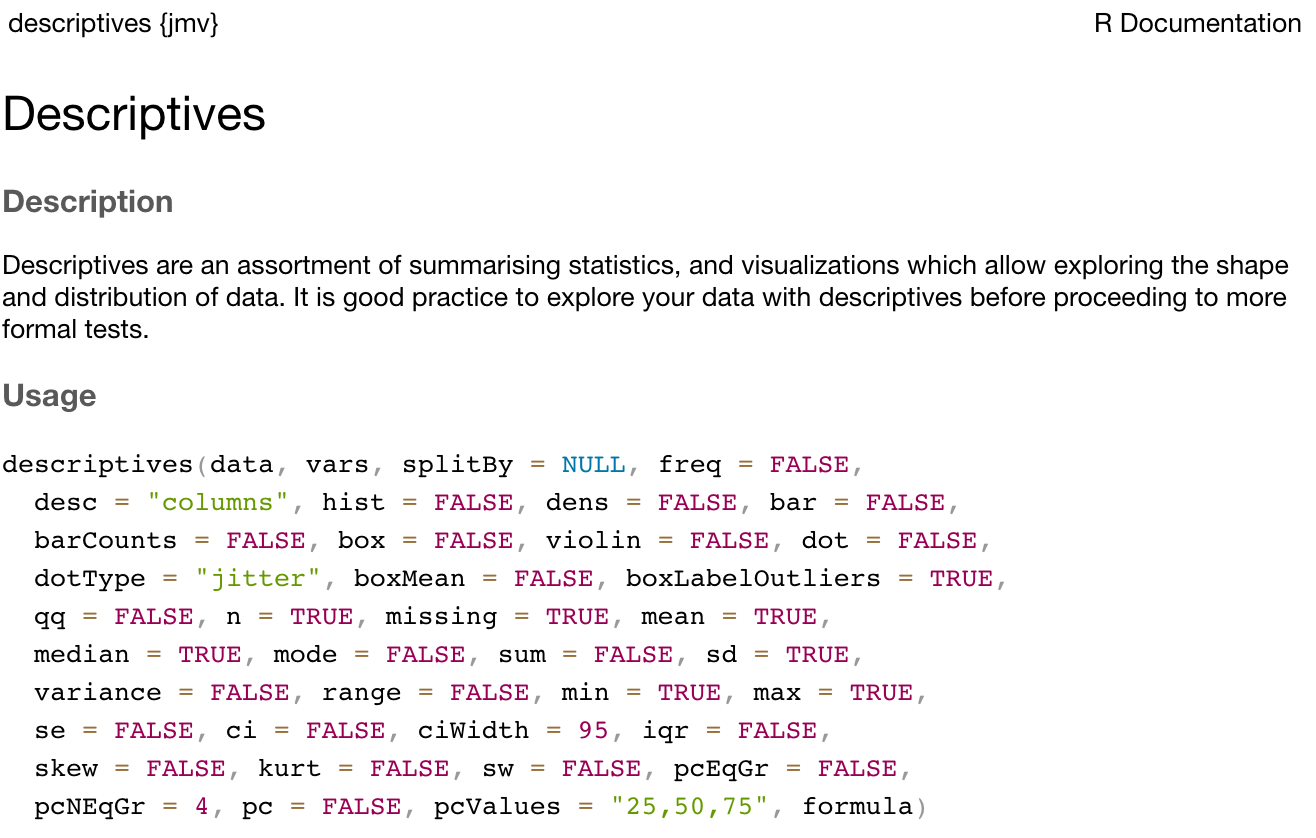
\includegraphics[width=0.8\linewidth,height=\textheight,keepaspectratio]{img/mod01/help-3.png}

There are two things to note here. First, notice that the first two
inputs are listed with no \texttt{=} symbol, but all other inputs are
listed with \texttt{=} symbols (with values provided after the
\texttt{=} symbol). This means that everything apart from \texttt{data}
and \texttt{vars} have \textbf{default} values. We are free to not
specify values for these inputs if we are happy with the defaults
provided. For example, by default the variance is not calculated (as
\texttt{variance\ =\ FALSE}). To obtain the variance as well as the
standard deviation, we can change this default to
\texttt{variance\ =\ TRUE}:

\begin{Shaded}
\begin{Highlighting}[]
\CommentTok{\# Only the standard deviation is provided as the measure of variability}
\FunctionTok{descriptives}\NormalTok{(}\AttributeTok{data =}\NormalTok{ pbc, }\AttributeTok{vars =}\NormalTok{ age)}

\CommentTok{\# Additionally request the variance to be calculated}
\FunctionTok{descriptives}\NormalTok{(}\AttributeTok{data =}\NormalTok{ pbc, }\AttributeTok{vars =}\NormalTok{ age, }\AttributeTok{variance =} \ConstantTok{TRUE}\NormalTok{)}
\end{Highlighting}
\end{Shaded}

Second, for functions with multiple inputs, we can specify the input
name and its value, or we can ignore the input name and specify just the
input values \textbf{in the order listed in the Usage section}. So the
following are equivalent:

\begin{Shaded}
\begin{Highlighting}[]
\CommentTok{\# We can specify that the dataset to be summarised is pbc,}
\CommentTok{\#   and the variable to summarise is age:}
\FunctionTok{descriptives}\NormalTok{(}\AttributeTok{data =}\NormalTok{ pbc, }\AttributeTok{vars =}\NormalTok{ age)}

\CommentTok{\# We can omit the input name, as long as we keep the inputs in the correct order {-}}
\CommentTok{\#   that is, dataset first, variable second:}
\FunctionTok{descriptives}\NormalTok{(pbc, age)}

\CommentTok{\# We can change the order of the inputs, as long as we specify the input name:}
\FunctionTok{descriptives}\NormalTok{(}\AttributeTok{vars =}\NormalTok{ age, }\AttributeTok{data =}\NormalTok{ pbc)}
\end{Highlighting}
\end{Shaded}

In this course, we will usually provide all the input names, even when
they are not required. As you become more familiar with R, you will
start to use the shortcut method.

\subsubsection{The curse of
inconsistency}\label{the-curse-of-inconsistency}

As R is an open-source project, many people have contributed to its
development. This has led to a frustrating part of R: some functions
require a single object to be specified, but some require you to specify
a data frame and select variables for analysis. Let's see an example.

The help for \texttt{summary()} specifies the usage as:
\texttt{summary(object,\ ...)}. This means we need to specify a single
object to be summarised. An object could be a single column of data
(i.e.~a vector), or it could be a data frame. If we have a data frame
called \texttt{pbc} which contains many variables, the command
\texttt{summary(pbc)} would summarise every variable in the data frame.

What if we only wanted to summarise the age of the participants in the
data frame? To select a single variable from a data frame, we can use
the following syntax: \texttt{dataframe\$variable}. So to summarise just
age from this data frame, we would use: \texttt{summary(pbc\$age)}.

Compare this with the \texttt{descriptives()} function in the
\texttt{jmv} package. We saw earlier that the two required inputs for
\texttt{descriptives()} are \texttt{data} (the data frame to be
analysed) and \texttt{vars} (the variables to be analysed). So to
summarise \texttt{age} from the \texttt{pbc} data frame, we would
specify \texttt{descriptives(data=pbc,\ vars=age)}.

This inconsistency will seem maddening at first, and will continue to be
maddening! Reading the \textbf{usage} section of the help pages is a
useful way to determine whether you should specify an object (like
\texttt{pbc\$age}) or a data frame and a list of variables.

\subsection{Packages}\label{packages}

A \textbf{package} is a collection of functions, documentation (and
sometimes datasets) that extend the capabilities of R. Packages have
been written by R users to be freely distributed and used by others. R
packages can be obtained from many sources, but the most common source
is CRAN: the Comprehensive R Archive Network.

A useful way of thinking about R is that R is like a smartphone, with
packages being like apps which are downloaded from CRAN (similar to an
app-store). When you first install R, it comes with a basic set of
packages (apps) installed. You can do a lot of things with these basic
packages, but sometimes you might want to do things differently, or you
may want to perform some analyses that can't be done using the default
packages. In these cases, you can install a package.

Like installing an app on a smartphone, you only need to \emph{install}
a package once. But each time you want to use the package, you need to
\emph{load} the package into R.

\subsubsection{How to install a package}\label{how-to-install-a-package}

There are a couple of ways to install a package. You can use the
\texttt{install.packages()} function if you know the exact name of the
package. Let's use an example of installing the \texttt{skimr} package,
which gives a very nice, high-level overview of any data frame. We can
install \texttt{skimr} by typing the following into the console:

\begin{Shaded}
\begin{Highlighting}[]
\FunctionTok{install.packages}\NormalTok{(}\StringTok{"skimr"}\NormalTok{)}
\end{Highlighting}
\end{Shaded}

Note the use of the quotation marks.

Alternatively, RStudio offers a graphical way of installing packages
that can be accessed via \textbf{Tools \textgreater{} Install Packages},
or via the \textbf{Install} button at the top of the \textbf{Packages}
tab in the bottom-right window. You can begin typing the name of the
package in the dialog box that appears, and RStudio will use predictive
text to offer possible packages:

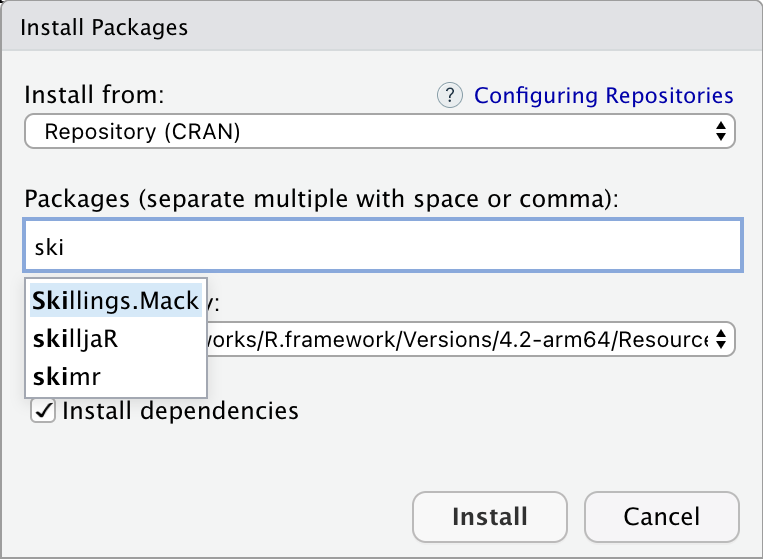
\includegraphics[width=0.6\linewidth,height=\textheight,keepaspectratio]{img/mod01/install-packages.png}

While writing code is usually the recommended way to use R, installing
packages is an exception. Using \textbf{Tools \textgreater{} Install
Packages} is perfectly fine, because you only need to install a package
once.

\subsubsection{How to load a package}\label{how-to-load-a-package}

When you begin a new session in RStudio, i.e.~when you open RStudio,
only certain core packages are automatically loaded. You can use the
\texttt{library()} function to load a package that has previously been
installed. For example, now that we have installed \texttt{skimr}, we
need to load it before we can use it:

\begin{Shaded}
\begin{Highlighting}[]
\FunctionTok{library}\NormalTok{(skimr)}
\end{Highlighting}
\end{Shaded}

Note that quotation marks are not required for the \texttt{library()}
function (although they can be included if you really like quotation
marks!). Another example of R's inconsistency!!!

\begin{tcolorbox}[enhanced jigsaw, arc=.35mm, bottomrule=.15mm, bottomtitle=1mm, breakable, colback=white, colbacktitle=quarto-callout-note-color!10!white, colframe=quarto-callout-note-color-frame, coltitle=black, left=2mm, leftrule=.75mm, opacityback=0, opacitybacktitle=0.6, rightrule=.15mm, title={TASK}, titlerule=0mm, toprule=.15mm, toptitle=1mm]

Install the packages \texttt{jmv} and \texttt{skimr} using \textbf{Tools
\textgreater{} Install packages}, or by typing into the console:

\texttt{install.packages("jmv")}

\texttt{install.packages("skimr")}

\end{tcolorbox}

\subsubsection{Installing vs loading
packages}\label{installing-vs-loading-packages}

Package installation:

\begin{itemize}
\tightlist
\item
  use the \texttt{install.packages()} function (note the `s') or
  \textbf{Tools \textgreater{} Install packages}
\item
  the package name must be surrounded by quotation marks
\item
  only needs to be done once
\end{itemize}

Package loading:

\begin{itemize}
\tightlist
\item
  use the \texttt{library()} function
\item
  the package name does not need to be surrounded by quotation marks
\item
  must be done for each R session
\end{itemize}

\subsection{What is this thing called the
tidyverse?}\label{what-is-this-thing-called-the-tidyverse}

If you have done much reading about R, you may have come across the
tidyverse:

\begin{quote}
``The tidyverse is an opinionated collection of R packages designed for
data science. All packages share an underlying design philosophy,
grammar, and data structures.'' \url{https://www.tidyverse.org/}
\end{quote}

Packages in the tidyverse have been designed with a goal to make using R
more consistent by defining a ``grammar'' to manipulate data, examine
data and draw conclusions from data. The tidyverse is a powerful set of
packages, and we will use only a small part of its capabilities.

More information about the tidyverse can be found using freely available
resources such as:
\href{https://jhudatascience.org/tidyversecourse/}{Tidyverse Skills for
Data Science} and \href{https://r4ds.had.co.nz/}{R for Data Science}.

\section{Part 2: Obtaining summary statistics for continuous
data}\label{part-2-obtaining-summary-statistics-for-continuous-data-1}

In this exercise (spanning Modules 1 and 2), we will analyse data to
complete a descriptive table from a research study. The data come from a
study in primary biliary cirrhosis, a condition of the liver, from
Modeling Survival Data: Extending the Cox Model by Therneau and Grambsch
(2010). By the end of this exercise, we will have completed some of
Table~\ref{tbl-r-t1}.

\begin{table}[h]

\caption{\label{tbl-r-t1}Summary of 418 participants from the PBC study
(Therneau and Grambsch, 2000)}

\centering{

\centering
\begin{talltblr}[         %% tabularray outer open
entry=none,label=none,
note{}={* aspartate aminotransferase},
]                     %% tabularray outer close
{                     %% tabularray inner open
colspec={Q[]Q[]Q[]},
hline{2}={1-3}{solid, black, 0.05em},
hline{1}={1-3}{solid, black, 0.08em},
hline{14}={1-3}{solid, black, 0.08em},
}                     %% tabularray inner close
Characteristic &   & Summary \\
Age (years) &   & Mean (SD) or Median [IQR] \\
Sex & Male & n (\%) \\
& Female & n (\%) \\
AST* (U/ml) &   & Mean (SD) or Median [IQR] \\
Serum bilirubin &   & Mean (SD) or Median [IQR] \\
Stage & I & n (\%) \\
& II & n (\%) \\
& III & n (\%) \\
& IIIV & n (\%) \\
Vital status at study end & Alive: no transplant & n (\%) \\
& Alive: transplant & n (\%) \\
& Deceased & n (\%) \\
\end{talltblr}

}

\end{table}%

This table is available in \texttt{Table1.docx}.

\begin{tcolorbox}[enhanced jigsaw, arc=.35mm, bottomrule=.15mm, bottomtitle=1mm, breakable, colback=white, colbacktitle=quarto-callout-note-color!10!white, colframe=quarto-callout-note-color-frame, coltitle=black, left=2mm, leftrule=.75mm, opacityback=0, opacitybacktitle=0.6, rightrule=.15mm, title={TASK}, titlerule=0mm, toprule=.15mm, toptitle=1mm]

Download the table shell, saved as \texttt{PBC\ Table1.docx}, and the
information file called \texttt{mod01\_pbc\_info.txt}.

\end{tcolorbox}

\subsection{Set up your data}\label{set-up-your-data}

We created a project in the previous step. We will now create a folder
to store all the data for this course. Storing the data within the
project makes life much easier!

Create a new folder by clicking the \textbf{New Folder} icon in the
\textbf{Files} tab at the bottom-right:

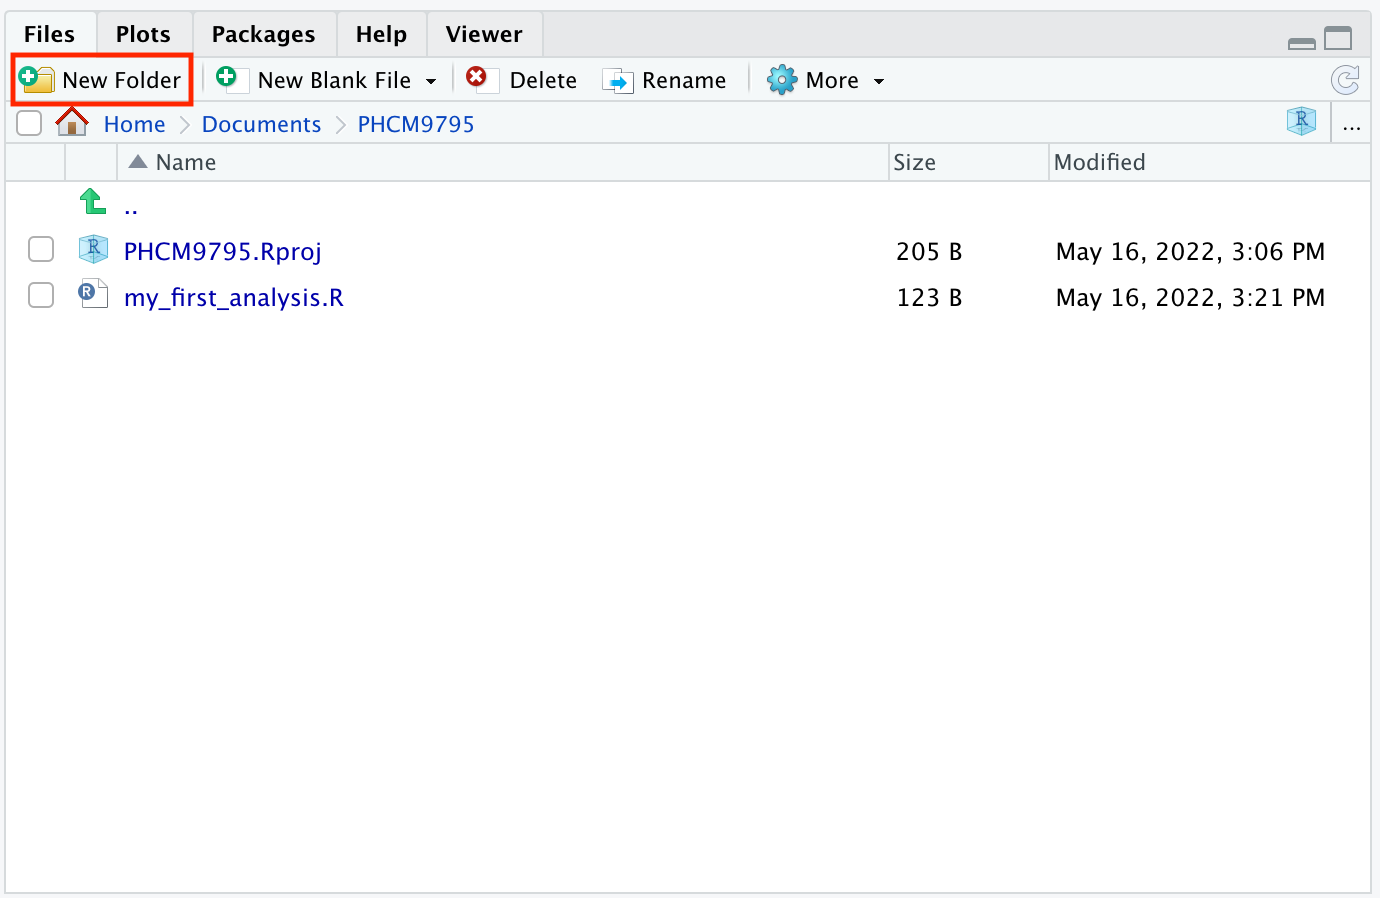
\includegraphics[width=0.75\linewidth,height=\textheight,keepaspectratio]{img/mod01/NewFolder-1.png}

Call the new folder \textbf{data}.

Click on this folder to open it, and then create two new folders:
\textbf{activities} and \textbf{examples}.

Download the ``Data sets: for learning activities'', and use Windows
Explorer or MacOS Finder to save these data sets in \textbf{activities}.
Save the ``Data sets: example data from course notes'' into the
\textbf{examples} folder.

Your \textbf{activities} folder should look like:

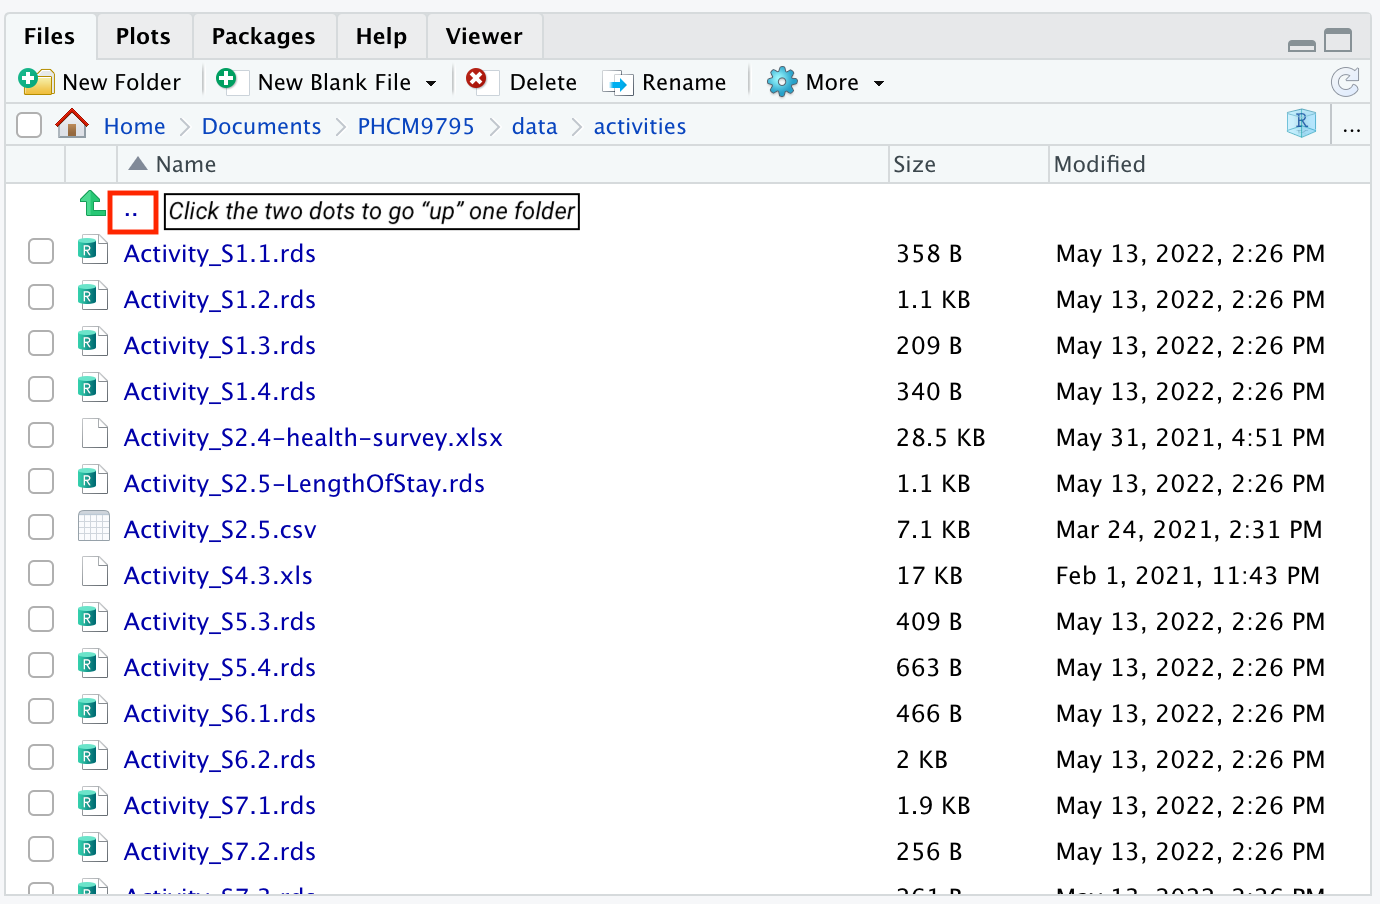
\includegraphics[width=0.75\linewidth,height=\textheight,keepaspectratio]{img/mod01/data-folder.png}

Click the two dots next to the up-arrow at the top of the folder
contents to move back up the folder structure. Note that you need to
click the dots, and not the up-facing green arrow!

\subsection{Reading a data file}\label{reading-a-data-file}

Typing data directly into R is not common; we usually read data that
have been previously saved. In this example, we will read an
\texttt{.rds} file using the \texttt{readRDS()} function, which has only
one input: the location of the file.

\begin{tcolorbox}[enhanced jigsaw, arc=.35mm, bottomrule=.15mm, bottomtitle=1mm, breakable, colback=white, colbacktitle=quarto-callout-note-color!10!white, colframe=quarto-callout-note-color-frame, coltitle=black, left=2mm, leftrule=.75mm, opacityback=0, opacitybacktitle=0.6, rightrule=.15mm, title={TASK}, titlerule=0mm, toprule=.15mm, toptitle=1mm]

1 - Confirm that the \texttt{mod01\_pdc.rds} file is in the
\texttt{activities} sub-folder within the \texttt{data} folder (as per
the previous steps).

2 - Load the \texttt{skimr} package, and use the \texttt{readRDS()}
function to read the file into R, assigning it to a data frame called
\texttt{pbc}. Because we set up our project, we can locate our data
easily by telling R to use the file:
\texttt{"data/activities/mod01\_pdc.rds"}, which translates as: the file
\texttt{mod01\_pdc.rds} which is located in the \texttt{activities}
sub-folder within the \texttt{data} folder.

\begin{Shaded}
\begin{Highlighting}[]
\FunctionTok{library}\NormalTok{(skimr)}

\NormalTok{pbc }\OtherTok{\textless{}{-}} \FunctionTok{readRDS}\NormalTok{(}\StringTok{"data/activities/mod01\_pbc.rds"}\NormalTok{)}
\end{Highlighting}
\end{Shaded}

3 - We can now use the \texttt{summary()} function to examine the pbc
dataset:

\begin{Shaded}
\begin{Highlighting}[]
\FunctionTok{summary}\NormalTok{(pbc)}
\end{Highlighting}
\end{Shaded}

\begin{verbatim}
       id             time          status            trt       
 Min.   :  1.0   Min.   :  41   Min.   :0.0000   Min.   :1.000  
 1st Qu.:105.2   1st Qu.:1093   1st Qu.:0.0000   1st Qu.:1.000  
 Median :209.5   Median :1730   Median :0.0000   Median :1.000  
 Mean   :209.5   Mean   :1918   Mean   :0.8301   Mean   :1.494  
 3rd Qu.:313.8   3rd Qu.:2614   3rd Qu.:2.0000   3rd Qu.:2.000  
 Max.   :418.0   Max.   :4795   Max.   :2.0000   Max.   :2.000  
                                                 NAs    :106    
      age             sex           ascites            hepato      
 Min.   :26.28   Min.   :1.000   Min.   :0.00000   Min.   :0.0000  
 1st Qu.:42.83   1st Qu.:2.000   1st Qu.:0.00000   1st Qu.:0.0000  
 Median :51.00   Median :2.000   Median :0.00000   Median :1.0000  
 Mean   :50.74   Mean   :1.895   Mean   :0.07692   Mean   :0.5128  
 3rd Qu.:58.24   3rd Qu.:2.000   3rd Qu.:0.00000   3rd Qu.:1.0000  
 Max.   :78.44   Max.   :2.000   Max.   :1.00000   Max.   :1.0000  
                                 NAs    :106       NAs    :106     
    spiders           edema             bili             chol       
 Min.   :0.0000   Min.   :0.0000   Min.   : 0.300   Min.   : 120.0  
 1st Qu.:0.0000   1st Qu.:0.0000   1st Qu.: 0.800   1st Qu.: 249.5  
 Median :0.0000   Median :0.0000   Median : 1.400   Median : 309.5  
 Mean   :0.2885   Mean   :0.1005   Mean   : 3.221   Mean   : 369.5  
 3rd Qu.:1.0000   3rd Qu.:0.0000   3rd Qu.: 3.400   3rd Qu.: 400.0  
 Max.   :1.0000   Max.   :1.0000   Max.   :28.000   Max.   :1775.0  
 NAs    :106                                        NAs    :134     
    albumin          copper          alkphos             ast        
 Min.   :1.960   Min.   :  4.00   Min.   :  289.0   Min.   : 26.35  
 1st Qu.:3.243   1st Qu.: 41.25   1st Qu.:  871.5   1st Qu.: 80.60  
 Median :3.530   Median : 73.00   Median : 1259.0   Median :114.70  
 Mean   :3.497   Mean   : 97.65   Mean   : 1982.7   Mean   :122.56  
 3rd Qu.:3.770   3rd Qu.:123.00   3rd Qu.: 1980.0   3rd Qu.:151.90  
 Max.   :4.640   Max.   :588.00   Max.   :13862.4   Max.   :457.25  
                 NAs    :108      NAs    :106       NAs    :106     
      trig           platelet        protime          stage      
 Min.   : 33.00   Min.   : 62.0   Min.   : 9.00   Min.   :1.000  
 1st Qu.: 84.25   1st Qu.:188.5   1st Qu.:10.00   1st Qu.:2.000  
 Median :108.00   Median :251.0   Median :10.60   Median :3.000  
 Mean   :124.70   Mean   :257.0   Mean   :10.73   Mean   :3.024  
 3rd Qu.:151.00   3rd Qu.:318.0   3rd Qu.:11.10   3rd Qu.:4.000  
 Max.   :598.00   Max.   :721.0   Max.   :18.00   Max.   :4.000  
 NAs    :136      NAs    :11      NAs    :2       NAs    :6      
\end{verbatim}

An alternative to the \texttt{summary()} function is the \texttt{skim()}
function in the \texttt{skimr} package, which produces summary
statistics as well as rudimentary histograms:

\begin{Shaded}
\begin{Highlighting}[]
\FunctionTok{skim}\NormalTok{(pbc)}
\end{Highlighting}
\end{Shaded}

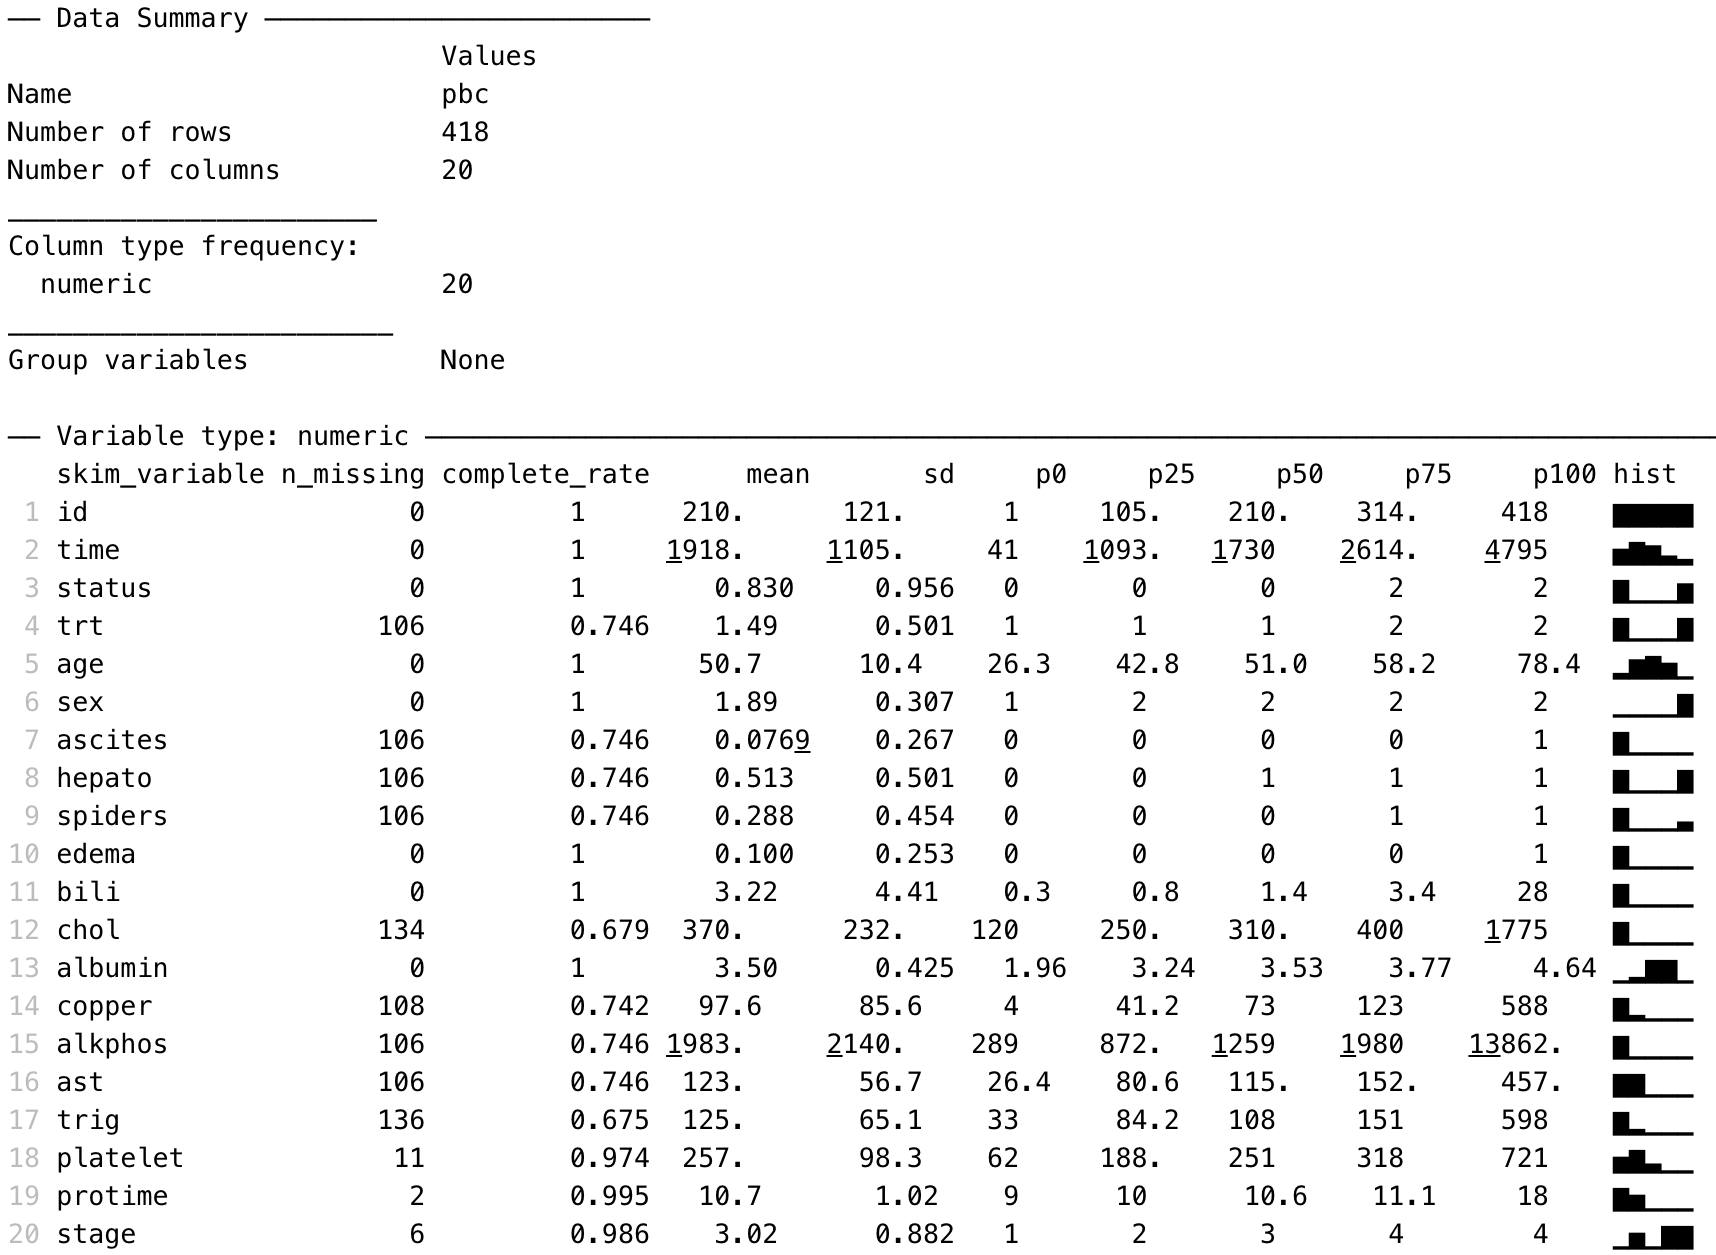
\includegraphics[width=0.9\linewidth,height=\textheight,keepaspectratio]{img/mod01/skim-pbc.png}

\end{tcolorbox}

The \texttt{summary()} and \texttt{skim()} functions are useful to give
a quick overview of a dataset: how many variables are included, how
variables are coded, which variables contain missing data and a crude
histogram showing the distribution of numeric variables.

\subsection{Summarising continuous
variables}\label{summarising-continuous-variables-1}

One of the most flexible functions for summarising continuous variables
is the \texttt{descriptives()} function from the \texttt{jmv} package.
The function is specified as \texttt{descriptives(data=,\ vars=)} where:

\begin{itemize}
\tightlist
\item
  \texttt{data} specifies the dataframe to be analysed
\item
  \texttt{vars} specifies the variable(s) of interest, with multiple
  variables combined using the \texttt{c()} function
\end{itemize}

We can summarise the three continuous variables in the pbc data: age,
AST and serum bilirubin, as shown below.

\begin{Shaded}
\begin{Highlighting}[]
\FunctionTok{library}\NormalTok{(jmv)}

\FunctionTok{descriptives}\NormalTok{(}\AttributeTok{data =}\NormalTok{ pbc, }\AttributeTok{vars =} \FunctionTok{c}\NormalTok{(age, ast, bili))}
\end{Highlighting}
\end{Shaded}

\begin{verbatim}

 DESCRIPTIVES

 Descriptives                                                
 ─────────────────────────────────────────────────────────── 
                         age         ast         bili        
 ─────────────────────────────────────────────────────────── 
   N                          418         312          418   
   Missing                      0         106            0   
   Mean                  50.74155    122.5563     3.220813   
   Median                51.00068    114.7000     1.400000   
   Standard deviation    10.44721    56.69952     4.407506   
   Minimum               26.27789    26.35000    0.3000000   
   Maximum               78.43943    457.2500     28.00000   
 ─────────────────────────────────────────────────────────── 
\end{verbatim}

By default, the \texttt{descriptives} function presents the mean,
median, standard deviation, minimum and maximum. We can request
additional statistics, such as the quartiles (which are called the
percentiles, or pc, in the descriptives function):

\begin{Shaded}
\begin{Highlighting}[]
\FunctionTok{descriptives}\NormalTok{(}\AttributeTok{data =}\NormalTok{ pbc, }\AttributeTok{vars =} \FunctionTok{c}\NormalTok{(age, ast, bili), }\AttributeTok{pc =} \ConstantTok{TRUE}\NormalTok{)}
\end{Highlighting}
\end{Shaded}

\begin{verbatim}

 DESCRIPTIVES

 Descriptives                                                
 ─────────────────────────────────────────────────────────── 
                         age         ast         bili        
 ─────────────────────────────────────────────────────────── 
   N                          418         312          418   
   Missing                      0         106            0   
   Mean                  50.74155    122.5563     3.220813   
   Median                51.00068    114.7000     1.400000   
   Standard deviation    10.44721    56.69952     4.407506   
   Minimum               26.27789    26.35000    0.3000000   
   Maximum               78.43943    457.2500     28.00000   
   25th percentile       42.83231    80.60000    0.8000000   
   50th percentile       51.00068    114.7000     1.400000   
   75th percentile       58.24093    151.9000     3.400000   
 ─────────────────────────────────────────────────────────── 
\end{verbatim}

\subsection{Producing a density plot}\label{producing-a-density-plot-1}

We can add \texttt{dens=TRUE} to the \texttt{descriptives} function to
produce a density plot for each listed variable:

\begin{Shaded}
\begin{Highlighting}[]
\FunctionTok{descriptives}\NormalTok{(}\AttributeTok{data =}\NormalTok{ pbc, }\AttributeTok{vars =} \FunctionTok{c}\NormalTok{(age, ast, bili), }\AttributeTok{pc =} \ConstantTok{TRUE}\NormalTok{, }\AttributeTok{dens =} \ConstantTok{TRUE}\NormalTok{)}
\end{Highlighting}
\end{Shaded}

\begin{verbatim}

 DESCRIPTIVES

 Descriptives                                                
 ─────────────────────────────────────────────────────────── 
                         age         ast         bili        
 ─────────────────────────────────────────────────────────── 
   N                          418         312          418   
   Missing                      0         106            0   
   Mean                  50.74155    122.5563     3.220813   
   Median                51.00068    114.7000     1.400000   
   Standard deviation    10.44721    56.69952     4.407506   
   Minimum               26.27789    26.35000    0.3000000   
   Maximum               78.43943    457.2500     28.00000   
   25th percentile       42.83231    80.60000    0.8000000   
   50th percentile       51.00068    114.7000     1.400000   
   75th percentile       58.24093    151.9000     3.400000   
 ─────────────────────────────────────────────────────────── 
\end{verbatim}

\pandocbounded{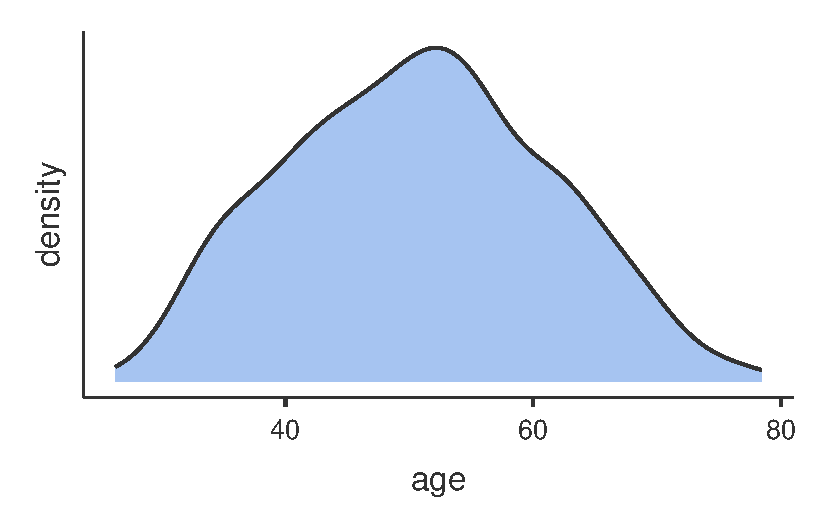
\includegraphics[keepaspectratio]{01-intro_files/figure-pdf/unnamed-chunk-32-1.pdf}}

\pandocbounded{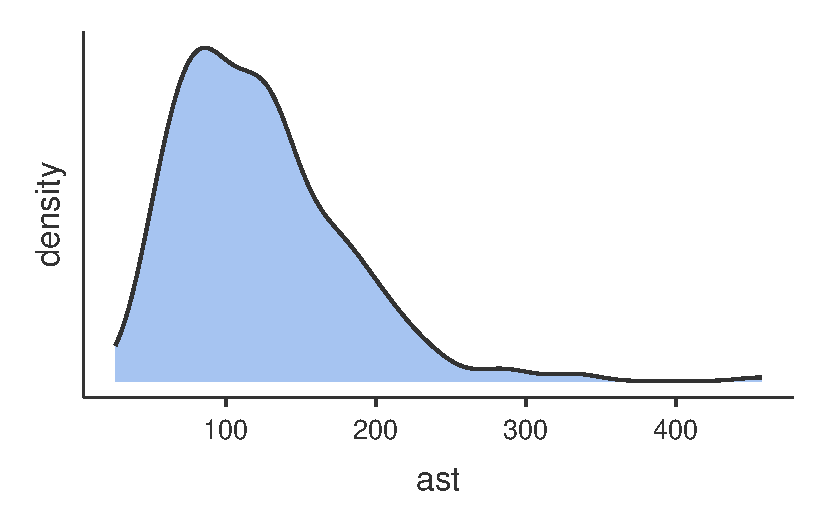
\includegraphics[keepaspectratio]{01-intro_files/figure-pdf/unnamed-chunk-32-2.pdf}}

\pandocbounded{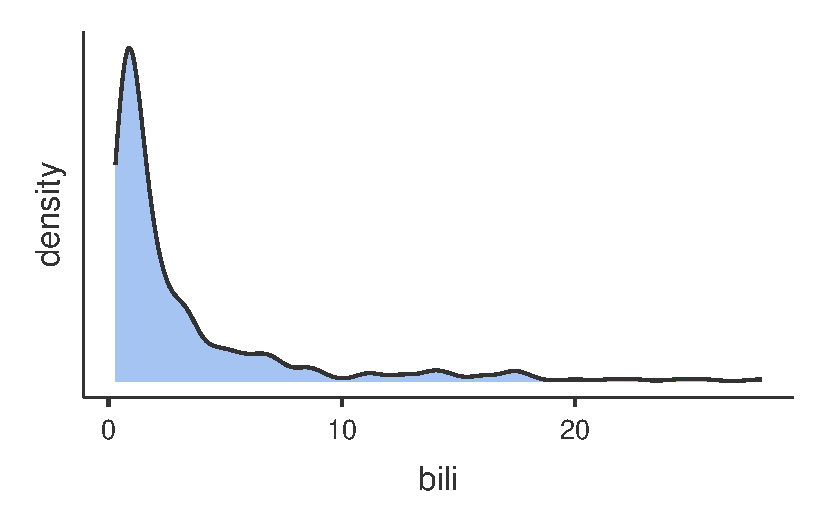
\includegraphics[keepaspectratio]{01-intro_files/figure-pdf/unnamed-chunk-32-3.pdf}}

Note that the density plots are plotted separately in the \textbf{Plot}
window. They can be viewed using the arrows at the top of the
\textbf{Plot} window:

\pandocbounded{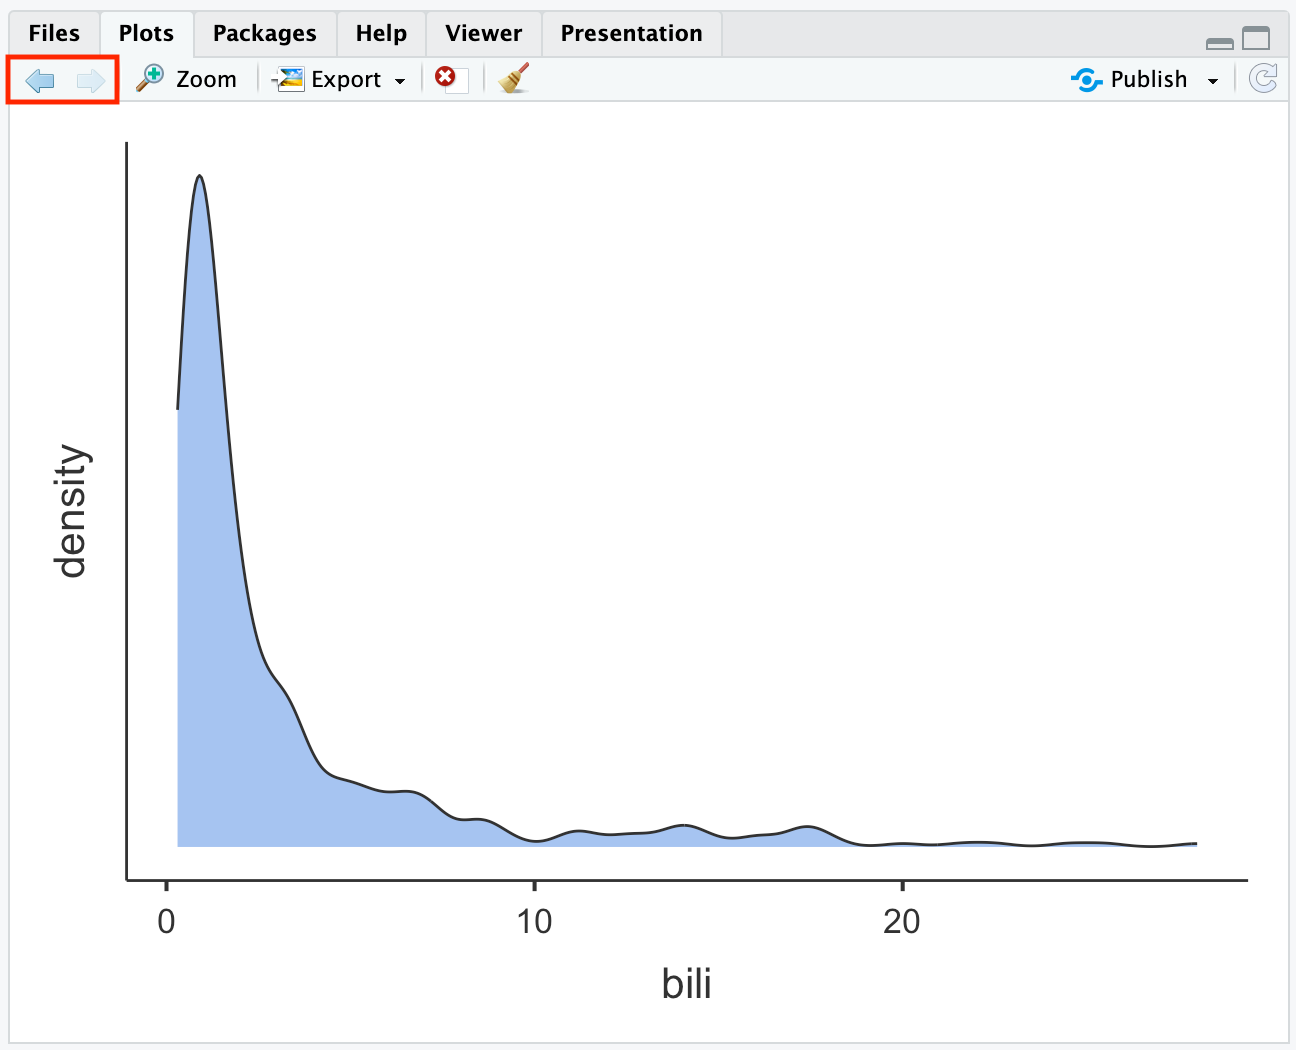
\includegraphics[keepaspectratio]{img/mod01/r-dens-01.png}}

A more flexible way of constructing a density plot is by using the
plot() function within R, using the syntax:
\texttt{plot(density(dataframe\$variable))}, which plots the
\texttt{variable} from the \texttt{dataframe}. For example, the default
density plot for the \texttt{age} column of the \texttt{pbc} data:

\begin{Shaded}
\begin{Highlighting}[]
\FunctionTok{plot}\NormalTok{(}\FunctionTok{density}\NormalTok{(pbc}\SpecialCharTok{$}\NormalTok{age))}
\end{Highlighting}
\end{Shaded}

\pandocbounded{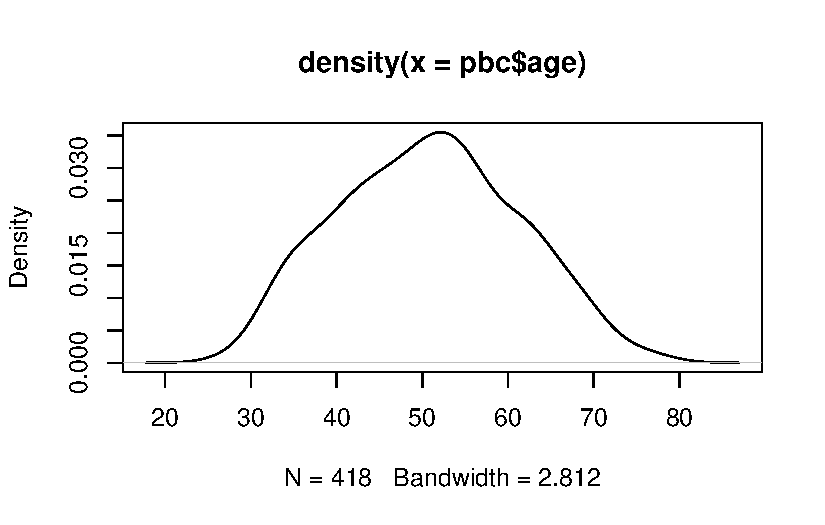
\includegraphics[keepaspectratio]{01-intro_files/figure-pdf/unnamed-chunk-33-1.pdf}}

This plot can be improved by using \texttt{xlab="\ "} and
\texttt{main="\ "} to assign labels for the x-axis and overall title
respectively:

\begin{Shaded}
\begin{Highlighting}[]
\FunctionTok{plot}\NormalTok{(}
  \FunctionTok{density}\NormalTok{(pbc}\SpecialCharTok{$}\NormalTok{age),}
  \AttributeTok{xlab =} \StringTok{"Age in years"}\NormalTok{,}
  \AttributeTok{main =} \StringTok{"Density plot of participant age from pbc study data"}
\NormalTok{)}
\end{Highlighting}
\end{Shaded}

\pandocbounded{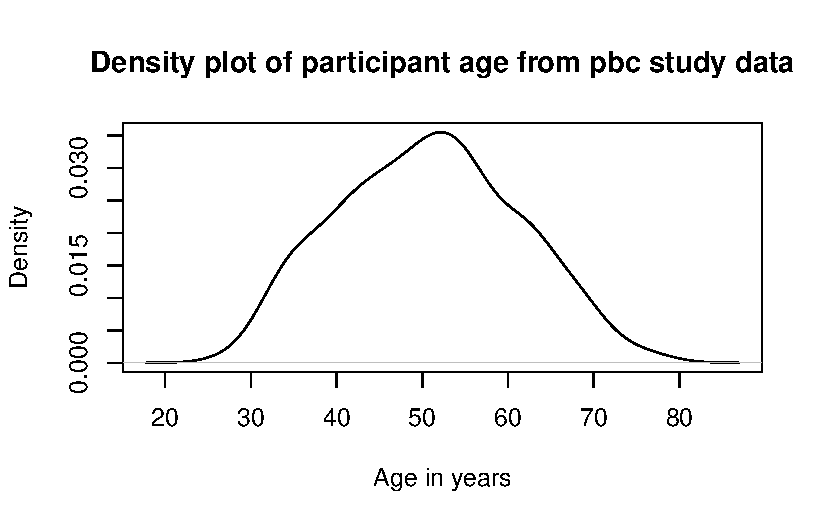
\includegraphics[keepaspectratio]{01-intro_files/figure-pdf/unnamed-chunk-34-1.pdf}}

\begin{tcolorbox}[enhanced jigsaw, arc=.35mm, bottomrule=.15mm, bottomtitle=1mm, breakable, colback=white, colbacktitle=quarto-callout-warning-color!10!white, colframe=quarto-callout-warning-color-frame, coltitle=black, left=2mm, leftrule=.75mm, opacityback=0, opacitybacktitle=0.6, rightrule=.15mm, title=\textcolor{quarto-callout-warning-color}{\faExclamationTriangle}\hspace{0.5em}{Note}, titlerule=0mm, toprule=.15mm, toptitle=1mm]

The \texttt{density()} function requires the analysis variable to
contain no missing values, and will give an error if there are any
missing values. We can use the option \texttt{na.rm=TRUE} to request
that the density function ignore any missing values. For example:

\begin{verbatim}
plot(density(pbc$ast, na.rm=TRUE),
     xlab="AST (U/mL)",
     main="Density plot of aspartate aminotransferase from pbc study data")
\end{verbatim}

\end{tcolorbox}

\subsection{Producing a boxplot}\label{producing-a-boxplot-1}

Like the density plot, boxplots can be requested in the
\texttt{descriptives} function by using \texttt{box=TRUE}.

The \texttt{boxplot} function is an alternative, more flexible function,
again specifying the dataframe to use and the variable to be plotted as
\texttt{dataframe\$variable}. Labels can be applied in the same way as
the histogram:

\begin{Shaded}
\begin{Highlighting}[]
\FunctionTok{boxplot}\NormalTok{(}
\NormalTok{  pbc}\SpecialCharTok{$}\NormalTok{age,}
  \AttributeTok{xlab =} \StringTok{"Age (years)"}\NormalTok{,}
  \AttributeTok{main =} \StringTok{"Boxplot of participant age from pbc study data"}
\NormalTok{)}
\end{Highlighting}
\end{Shaded}

\pandocbounded{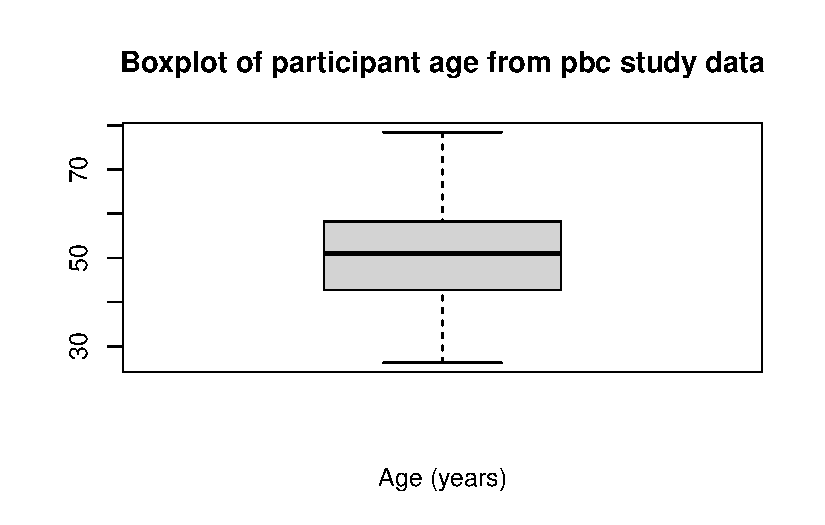
\includegraphics[keepaspectratio]{01-intro_files/figure-pdf/unnamed-chunk-35-1.pdf}}

\begin{tcolorbox}[enhanced jigsaw, arc=.35mm, bottomrule=.15mm, bottomtitle=1mm, breakable, colback=white, colbacktitle=quarto-callout-note-color!10!white, colframe=quarto-callout-note-color-frame, coltitle=black, left=2mm, leftrule=.75mm, opacityback=0, opacitybacktitle=0.6, rightrule=.15mm, title={TASK}, titlerule=0mm, toprule=.15mm, toptitle=1mm]

Obtain density plots and boxplots for age, AST and bilirubin.

Based on these plots, decide whether the mean or the median is the
appropriate summary to use for each variable.

\end{tcolorbox}

\subsection{Saving data in R}\label{saving-data-in-r}

There are many ways to save data from R, depending on the type of file
you want to save. The recommendation for this course is to save your
data using the \texttt{.rds} format, using the \texttt{saveRDS()}
function, which takes two inputs: \texttt{saveRDS(object,\ file)}. Here,
\texttt{object} is the R object to be saved (usually a data frame), and
\texttt{file} is the location for the file to be saved (file name and
path, including the \texttt{.rds} suffix).

It is not necessary to save our PBC data, as we have made only minor
changes to the data that can be replicated by rerunning our script. If
you had made major changes and wanted to save your data, you could use:

\texttt{saveRDS(pbc,\ file="pbc\_revised.rds")}

\subsection{Copying output from R}\label{copying-output-from-r}

It is important to note that saving your data or your script in R will
not save your output. The easiest way to retain the output of your
analyses is to copy the output from the Console into a word processor
package (e.g.~Microsoft Word) before closing R.

Unfortunately, by default, R is not ideal for creating publication
quality tables. There are many packages that will help in this process,
such as R Markdown, huxtable, gt and gtsummary, but their use is beyond
the scope of this course. \href{https://rmd4sci.njtierney.com/}{R
Markdown for Scientists} provides an excellent introduction to R
Markdown.

\begin{tcolorbox}[enhanced jigsaw, arc=.35mm, bottomrule=.15mm, bottomtitle=1mm, breakable, colback=white, colbacktitle=quarto-callout-note-color!10!white, colframe=quarto-callout-note-color-frame, coltitle=black, left=2mm, leftrule=.75mm, opacityback=0, opacitybacktitle=0.6, rightrule=.15mm, title={TASK}, titlerule=0mm, toprule=.15mm, toptitle=1mm]

Complete Table 1 for continuous variables using the output generated in
this exercise. You should decide on whether to present continuous
variables by their means or medians, and present the most appropriate
measure of spread. Include footnotes to indicate if any variables
contain missing observations.

\end{tcolorbox}

\section{Setting a value to missing}\label{setting-a-value-to-missing-1}

As we saw in Section~\ref{sec-eda-cts}, it is important to explore our
data to identify any unusual observations. If an error is found, the
best method for correcting the error is to go back to the original data
e.g.~the hard copy questionnaire, to obtain the original value, entering
the correct value into R. If the original data is not available or the
original data is also incorrect, the erroneous value is often excluded
from the dataset.

Consider a sample dataset: \texttt{mod01\_weight\_1000.rds}, which
contains the weights of 1000 people. A density plot and a boxplot should
be examined before we start analysing these data:

\pandocbounded{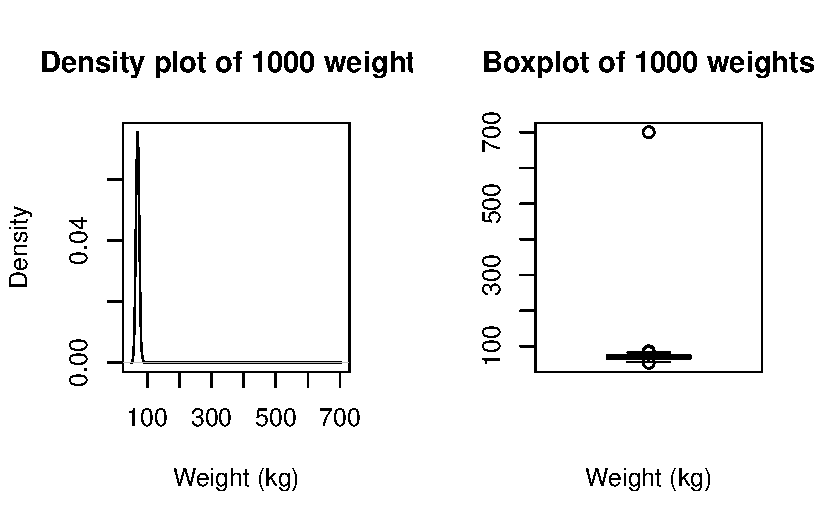
\includegraphics[keepaspectratio]{01-intro_files/figure-pdf/unnamed-chunk-36-1.pdf}}

There is a clear outlying point shown in the boxplot. Although not
obvious, the same point is shown in the density plot as a small blip
around 700kg. Obviously this point is unusual, and we should
investigate.

We can view any outlying observations in the dataset using the
\texttt{subset} function. You will need to decide if these values are a
data entry error or are biologically plausible. If an extreme value or
``outlier'', is biologically plausible, it should be included in all
analyses.

For example, to list any observations from the \texttt{sample} dataset
with a weight larger than 200:

\begin{Shaded}
\begin{Highlighting}[]
\FunctionTok{subset}\NormalTok{(sample, weight }\SpecialCharTok{\textgreater{}} \DecValTok{200}\NormalTok{)}
\end{Highlighting}
\end{Shaded}

\begin{verbatim}
   id weight
58 58  700.2
\end{verbatim}

We see that there is a very high value of 700.2kg. A value as high as
700kg is likely to be a data entry error (e.g.~error in entering an
extra zero) and is not a plausible weight value. Here, \textbf{you
should check your original data}.

If you do not have access to the original data, it would be safest to
set this value as missing. You do change this in R by using an
\texttt{ifelse} statement to recode the incorrect weight of 700.2kg into
a missing value. \textbf{A missing value in R is represented by NA}.

The form of the \texttt{ifelse} statement is as follows:
\texttt{ifelse(test,\ value\_if\_true,\ value\_if\_false)}

We will write code to:

\begin{itemize}
\tightlist
\item
  create a new column (called \texttt{weight\_clean}) in the
  \texttt{sample} dataframe (i.e.~\texttt{sample\$weight\_clean})
\item
  test whether \texttt{weight} is equal to 700.2

  \begin{itemize}
  \tightlist
  \item
    if this is true, we will assign \texttt{weight\_clean} to be NA
  \item
    otherwise \texttt{weight\_clean} will equal the value of
    \texttt{weight}
  \end{itemize}
\end{itemize}

Putting it all together:

\begin{Shaded}
\begin{Highlighting}[]
\NormalTok{sample}\SpecialCharTok{$}\NormalTok{weight\_clean }\OtherTok{=} \FunctionTok{ifelse}\NormalTok{(sample}\SpecialCharTok{$}\NormalTok{weight }\SpecialCharTok{==} \FloatTok{700.2}\NormalTok{, }\ConstantTok{NA}\NormalTok{, sample}\SpecialCharTok{$}\NormalTok{weight)}
\end{Highlighting}
\end{Shaded}

\textbf{Note:} if an extreme value lies within the range of biological
possibility it should not be set to missing.

The same syntax could be used to replace the incorrect value with the
correct value. For example, if you do source the original medical
records, you might find that the original weight was recorded in medical
records as 70.2kg. We could use simlar syntax to replace 700.2 by 70.2:
\texttt{sample\$weight\_clean\ =\ ifelse(sample\$weight==700.2,\ 70.2,\ sample\$weight)}

Once you have checked your data for errors, you are ready to start
analysing your data.

\subsection{What on earth: == ?}\label{what-on-earth}

In R, the test of equality is denoted by two equal signs: \texttt{==}.
So we would use \texttt{==} to test whether an observation is equal to a
certain value. Let's see an example:

\begin{Shaded}
\begin{Highlighting}[]
\CommentTok{\# Test whether 6 is equal to 6}
\DecValTok{6} \SpecialCharTok{==} \DecValTok{6}
\end{Highlighting}
\end{Shaded}

\begin{verbatim}
[1] TRUE
\end{verbatim}

\begin{Shaded}
\begin{Highlighting}[]
\CommentTok{\# Test whether 6 is equal to 42}
\DecValTok{6} \SpecialCharTok{==} \DecValTok{42}
\end{Highlighting}
\end{Shaded}

\begin{verbatim}
[1] FALSE
\end{verbatim}

You can read the \texttt{==} as ``is equal to''. So the code
\texttt{sample\$weight\ ==\ 700.2} is read as: ``is the value of weight
from the data frame sample equal to 700.2?''. In our \texttt{ifelse}
statement above, if this condition is true, we replace \texttt{weight}
by 70.2; if it is false, we leave weight as is.

\newpage{}

\bookmarksetup{startatroot}

\chapter*{Activities}\label{activities}
\addcontentsline{toc}{chapter}{Activities}

\markboth{Activities}{Activities}

\subsection*{Activity 1.1}\label{activity-1.1}
\addcontentsline{toc}{subsection}{Activity 1.1}

25 participants were enrolled in a 3-week weight loss program.
Table~\ref{tbl-wt-loss} presents the weight loss (in grams) of the
participants.

\begin{table}[H]

\caption{\label{tbl-wt-loss}Weight loss (g) for 25 participants}

\centering{

\centering
\begin{tblr}[         %% tabularray outer open
]                     %% tabularray outer close
{                     %% tabularray inner open
colspec={Q[]Q[]Q[]Q[]Q[]},
hline{1}={1-5}{solid, black, 0.08em},
hline{6}={1-5}{solid, black, 0.08em},
}                     %% tabularray inner close
255 & 198 & 283 & 312 & 283 \\
57 & 85 & 312 & 142 & 113 \\
227 & 283 & 255 & 340 & 142 \\
113 & 312 & 227 & 85 & 170 \\
255 & 198 & 113 & 227 & 255 \\
\end{tblr}

}

\end{table}%

\begin{enumerate}
\def\labelenumi{\alph{enumi})}
\tightlist
\item
  These data have been saved as \texttt{Activity\_1.1.rds}. Read the
  data into your software package.
\item
  What type of data are these?
\item
  Construct an appropriate graph to display the distribution of
  participants' weight loss. Provide appropriate labels for the axes and
  give the graph an appropriate title.
\end{enumerate}

\subsection*{Activity 1.2}\label{activity-1.2}
\addcontentsline{toc}{subsection}{Activity 1.2}

Which of the following statements are true? The more dispersed, or
spread out, a set of observations are:

\begin{enumerate}
\def\labelenumi{\alph{enumi})}
\tightlist
\item
  The smaller the mean value
\item
  The larger the standard deviation
\item
  The smaller the variance
\end{enumerate}

\subsection*{Activity 1.3}\label{activity-1.3}
\addcontentsline{toc}{subsection}{Activity 1.3}

A study was conducted to investigate the general health of undergraduate
students at Australian universities. A random selection of 218 UNSW
undergradute students from UNSW were enrolled, and their diastolic blood
pressures are provided in the dataset \texttt{Activity\_1.3.csv}.
Compute the mean, median, range and standard deviation of diastolic
blood pressure.

\subsection*{Activity 1.4}\label{activity-1.4}
\addcontentsline{toc}{subsection}{Activity 1.4}

The ages of 100 study participants have been saved as
\texttt{Activity\_1.4.rds}. Estimate the:

\begin{enumerate}
\def\labelenumi{\alph{enumi}.}
\tightlist
\item
  mean and median;
\item
  standard deviation and interquartile range;
\item
  range.
\end{enumerate}

Plot the data. Is there anything unusual about the ages? What do you
think is a possible explanation for this?

A clean version of the data have been saved as
\texttt{Activity\_1.4\_clean.rds}. Recalculate the summary statistics
and recreate the plots using the clean data.

Based on this exercise, what is your advice on coding unusual or missing
values in data?

\bookmarksetup{startatroot}

\chapter{Categorical data, presentation guidelines and probability
distributions}\label{categorical-data-presentation-guidelines-and-probability-distributions}

\section*{Learning objectives}\label{learning-objectives-1}
\addcontentsline{toc}{section}{Learning objectives}

\markright{Learning objectives}

By the end of this module you will be able to:

\begin{itemize}
\tightlist
\item
  Present and report categorical data numerically and graphically
\item
  Describe the concept of probability
\item
  Describe the characteristics of a binomial distribution
\item
  Compute probabilities from a binomial distribution using statistical
  software
\end{itemize}

\section*{Optional readings}\label{optional-readings-1}
\addcontentsline{toc}{section}{Optional readings}

\markright{Optional readings}

Kirkwood and Sterne (2001); Chapters 3, 14 and 15.
\href{http://er1.library.unsw.edu.au/er/cgi-bin/eraccess.cgi?url=https://ebookcentral.proquest.com/lib/unsw/detail.action?docID=624728}{{[}UNSW
Library Link{]}}

Bland (2015); Chapters 5 and 6.
\href{http://er1.library.unsw.edu.au/er/cgi-bin/eraccess.cgi?url=https://ebookcentral.proquest.com/lib/unsw/detail.action?docID=5891730}{{[}UNSW
Library Link{]}}

Graphics and statistics for cardiology: designing effective tables for
presentation and publication, Boers (2018,
\href{https://er1.library.unsw.edu.au/er/cgi-bin/eraccess.cgi?url=http://dx.doi.org/10.1136/heartjnl-2017-311581}{UNSW
Library Link})

Guidelines for Reporting of Figures and Tables for Clinical Research in
Urology, Vickers et al. (2020,
\href{https://er1.library.unsw.edu.au/er/cgi-bin/eraccess.cgi?url=http://dx.doi.org/10.1016/j.eururo.2020.04.048}{UNSW
Library Link})

\section{Introduction}\label{introduction-1}

In Module 1, we saw how to summarise continuous data numerically and
graphically. In this module, we will show how to summarise categorical
data numerically and graphically. We will also introduce the concept of
probability which underpins the theoretical basis of statistics, and
then introduce the concept of probability distributions. We will present
the binomial distribution, which calculates the probability of observing
a certain number of events from multiple observations.

\section{Summarising a single categorical variable
numerically}\label{summarising-a-single-categorical-variable-numerically}

Categorical data are best summarised using a frequency table, where each
category is summarised by its frequency: the count of the number of
individuals in each category. The \textbf{relative frequency} (the
frequency expressed as a proportion or percentage of the total
frequency) is usually included give further insight.

\begin{table}[h]

\caption{\label{tbl-1-sex}Sex of participants in PBC study}

\centering{

\centering
\begin{tblr}[         %% tabularray outer open
]                     %% tabularray outer close
{                     %% tabularray inner open
colspec={Q[]Q[]Q[]},
hline{2}={1-3}{solid, black, 0.05em},
hline{1}={1-3}{solid, black, 0.08em},
hline{4}={1-3}{solid, black, 0.08em},
column{2-3}={}{halign=c},
column{1}={}{halign=l},
}                     %% tabularray inner close
Sex & Frequency & Relative frequency (\%) \\
Male & 44 & 10.5 \\
Female & 374 & 89.5 \\
\end{tblr}

}

\end{table}%

It is sometimes useful to present the cumulative relative frequency,
which shows the relative frequency of individuals in a certain category
or below (for example, Table~\ref{tbl-1-stage}).

\begin{table}[h]

\caption{\label{tbl-1-stage}Stage of disease for participants in PBC
study}

\centering{

\centering
\begin{tblr}[         %% tabularray outer open
]                     %% tabularray outer close
{                     %% tabularray inner open
colspec={Q[]Q[]Q[]Q[]},
hline{2}={1-4}{solid, black, 0.05em},
hline{1}={1-4}{solid, black, 0.08em},
hline{6}={1-4}{solid, black, 0.08em},
column{2-4}={}{halign=c},
column{1}={}{halign=l},
}                     %% tabularray inner close
Stage of disease & Frequency & Relative frequency (\%) & Cumulative relative frequency (\%) \\
Stage 1 & 21 & 5.1 & 5.1 \\
Stage 2 & 92 & 22.3 & 27.4 \\
Stage 3 & 155 & 37.6 & 65.0 \\
Stage 4 & 144 & 35.0 & 100.0 \\
\end{tblr}

}

\end{table}%

From Table~\ref{tbl-1-stage}, we can see that 65.0\% of participants had
Stage 3 disease or lower.

\section{Summarising a single categorical variable
graphically}\label{summarising-a-single-categorical-variable-graphically}

A categorical variable is best summarised graphically using a
\textbf{bar chart}. For example, we can present the distribution of
Stage of Disease graphically using a bar graph (Figure~\ref{fig-bar-1}).
Bar graphs, which are suitable for plotting discrete or categorical
variables, are defined by the fact that the bars do not touch.

\begin{figure}[H]

\centering{

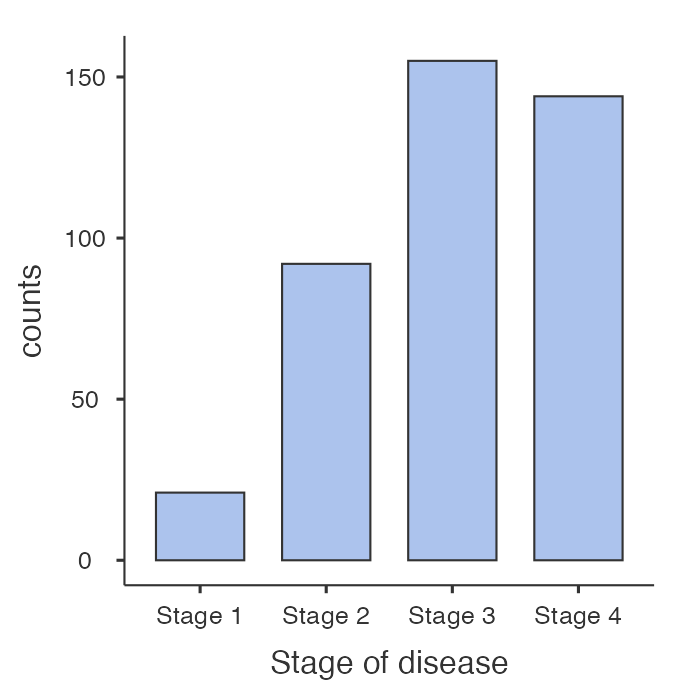
\includegraphics[width=0.75\linewidth,height=\textheight,keepaspectratio]{img/mod01/pbc-bar.png}

}

\caption{\label{fig-bar-1}Bar graph of stage of disease from PBC study}

\end{figure}%

Pie charts can be an alternative way to summarise a categorical variable
graphically, however their use is not recommended for the following
reasons:

\begin{itemize}
\tightlist
\item
  Not ideal when there are many categories to compare
\item
  The use of percentages is not appropriate when the sample size is
  small
\item
  Can be misleading by using different size pies, different rotations
  and different colours to draw attention to specific groups
\item
  3D and exploding bar charts further distort the effect of perspective
  and may confuse the reader
\end{itemize}

Pie charts will not be discussed further in this course.

\section{Exploratory data analysis for categorical
data}\label{sec-eda-cat}

As with continuous data, it is good practice to undertake exploratory
data analysis before formally analysing categorical data. You should
take a moment and examine a frequency table for categorical variables,
to ensure all recorded values are within scope.

\section{Summarising two categorical variables
numerically}\label{summarising-two-categorical-variables-numerically}

So far, we have discussed one-way frequency tables, that is, tables that
summarise one variable. We can summarise more than two categorical
variables in a table -- called a cross tabulation, or a two-way
(summarising two variables) table.

Using our PBC data, we can summarise the two categorical variables: sex
and stage of disease. The two-way table of frequencies is shown in
Table~\ref{tbl-1-sex-stage-freq}.

\begin{table}[h]

\caption{\label{tbl-1-sex-stage-freq}Frequency of participants by sex
and stage of disease*}

\centering{

\centering
\begin{talltblr}[         %% tabularray outer open
entry=none,label=none,
note{}={* Stage of disease was missing for 6 participants},
]                     %% tabularray outer close
{                     %% tabularray inner open
colspec={Q[]Q[]Q[]Q[]Q[]Q[]Q[]},
hline{2}={1-7}{solid, black, 0.05em},
hline{1}={1-7}{solid, black, 0.08em},
hline{5}={1-7}{solid, black, 0.08em},
column{1-2}={}{halign=l},
column{3-7}={}{halign=r},
}                     %% tabularray inner close
Sex &   & Stage 1 & Stage 2 & Stage 3 & Stage 4 & All \\
Male & Count & 3 & 8 & 16 & 17 & 44 \\
Female & Count & 18 & 84 & 139 & 127 & 374 \\
All & Count & 21 & 92 & 155 & 144 & 418 \\
\end{talltblr}

}

\end{table}%

We can add percentages to two-way tables as either \emph{column} or
\emph{row} percents. Using Table~\ref{tbl-1-sex-stage-freq} as an
example, column percents represent the relative frequencies of sex
within each stage (Table~\ref{tbl-1-sex-stage-col}).

\begin{table}[h]

\caption{\label{tbl-1-sex-stage-col}Frequency of participants by sex and
stage of disease*, including column percents}

\centering{

\centering
\begin{talltblr}[         %% tabularray outer open
entry=none,label=none,
note{}={* Stage of disease was missing for 6 participants},
]                     %% tabularray outer close
{                     %% tabularray inner open
colspec={Q[]Q[]Q[]Q[]Q[]Q[]},
hline{2}={1-6}{solid, black, 0.05em},
hline{1}={1-6}{solid, black, 0.08em},
hline{8}={1-6}{solid, black, 0.08em},
}                     %% tabularray inner close
Sex &   & Stage 1 & Stage 2 & Stage 3 & Stage 4 \\
Male & Count & 3 & 8 & 16 & 17 \\
& Column percent & 14.3 & 8.7 & 10.3 & 11.8 \\
Female & Count & 18 & 84 & 139 & 127 \\
& Column percent & 85.7 & 91.3 & 89.7 & 88.2 \\
All & Count & 21 & 92 & 155 & 144 \\
& Column percent & 100.0 & 100.0 & 100.0 & 100.0 \\
\end{talltblr}

}

\end{table}%

Conversely, row percents represent the relative frequencies of stage
within each sex (Table~\ref{tbl-1-sex-stage-row}).

\begin{table}[h]

\caption{\label{tbl-1-sex-stage-row}Frequency of participants by sex and
stage of disease*, including row percents}

\centering{

\centering
\begin{talltblr}[         %% tabularray outer open
entry=none,label=none,
note{}={* Stage of disease was missing for 6 participants},
]                     %% tabularray outer close
{                     %% tabularray inner open
colspec={Q[]Q[]Q[]Q[]Q[]Q[]Q[]},
hline{2}={1-7}{solid, black, 0.05em},
hline{1}={1-7}{solid, black, 0.08em},
hline{8}={1-7}{solid, black, 0.08em},
}                     %% tabularray inner close
Sex &   & Stage 1 & Stage 2 & Stage 3 & Stage 4 & All \\
Male & Count & 3 & 8 & 16 & 17 & 44 \\
& Row percent & 6.8 & 18.2 & 36.4 & 38.6 & 100.0 \\
Female & Count & 18 & 84 & 139 & 127 & 374 \\
& Row percent & 4.8 & 22.5 & 37.2 & 34.0 & 100.0 \\
All & Count & 21 & 92 & 155 & 144 & 418 \\
& Row percent & 5.0 & 22.0 & 37.1 & 34.4 & 100.0 \\
\end{talltblr}

}

\end{table}%

\newpage

\subsection{Tables containing more than two
variables}\label{tables-containing-more-than-two-variables}

It is possible to construct multi-way tables that summarise more than
two categorical variables in a single table. However, tables can become
complex when more than two variables are incorporated, and you may need
to present the information as two tables or incorporate additional rows
and columns.

In Figure~\ref{fig-1-2}, characteristics of the sample of prisoners from
the NPHDC were presented. This table contains information about sex, age
group and Indigenous status from different groups of prisoners; prison
entrants, discharges, and prisoners in custody. This type of condensed
information is often found in reports and journal articles giving
demographic information, by different groups considered in the study.

\begin{figure}

\centering{

\pandocbounded{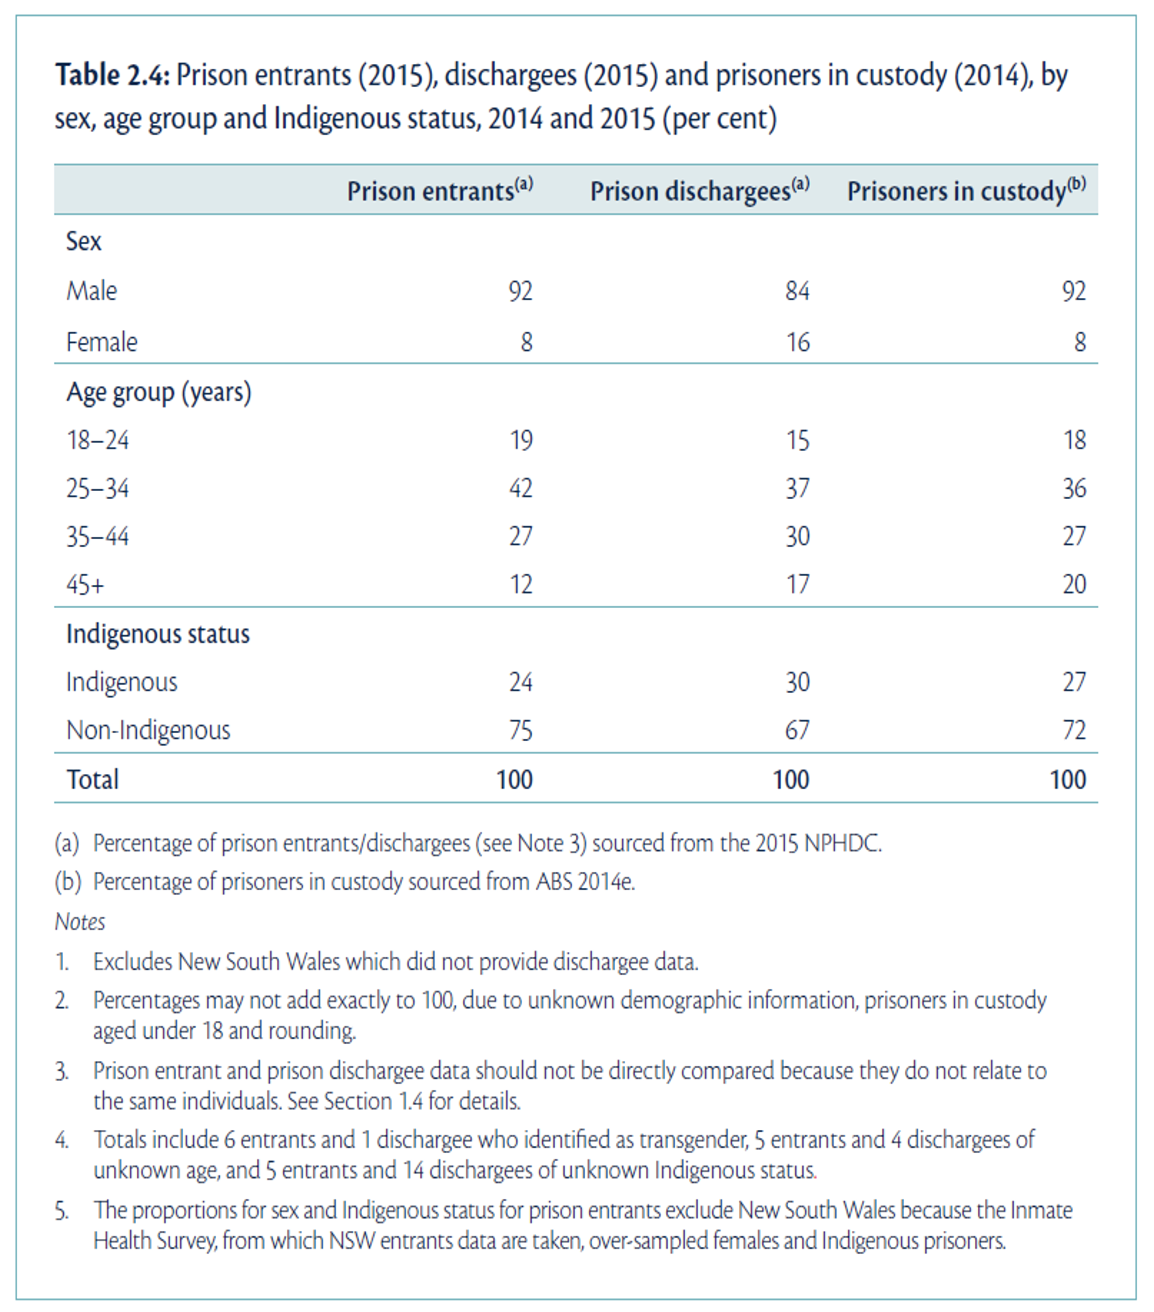
\includegraphics[keepaspectratio]{img/mod01/prisoner-health.png}}

}

\caption{\label{fig-1-2}}

\end{figure}%

We might also consider a table containing further pieces of information.
The table presented in Figure~\ref{fig-prison-education} (from the
health of Australia's prisoners 2015 report) compares prison entrants
and the general community by three variables: age group, Indigenous
status, and highest level of completed education.

Can you see any issues with the presentation of this table?

\begin{figure}[H]

\centering{

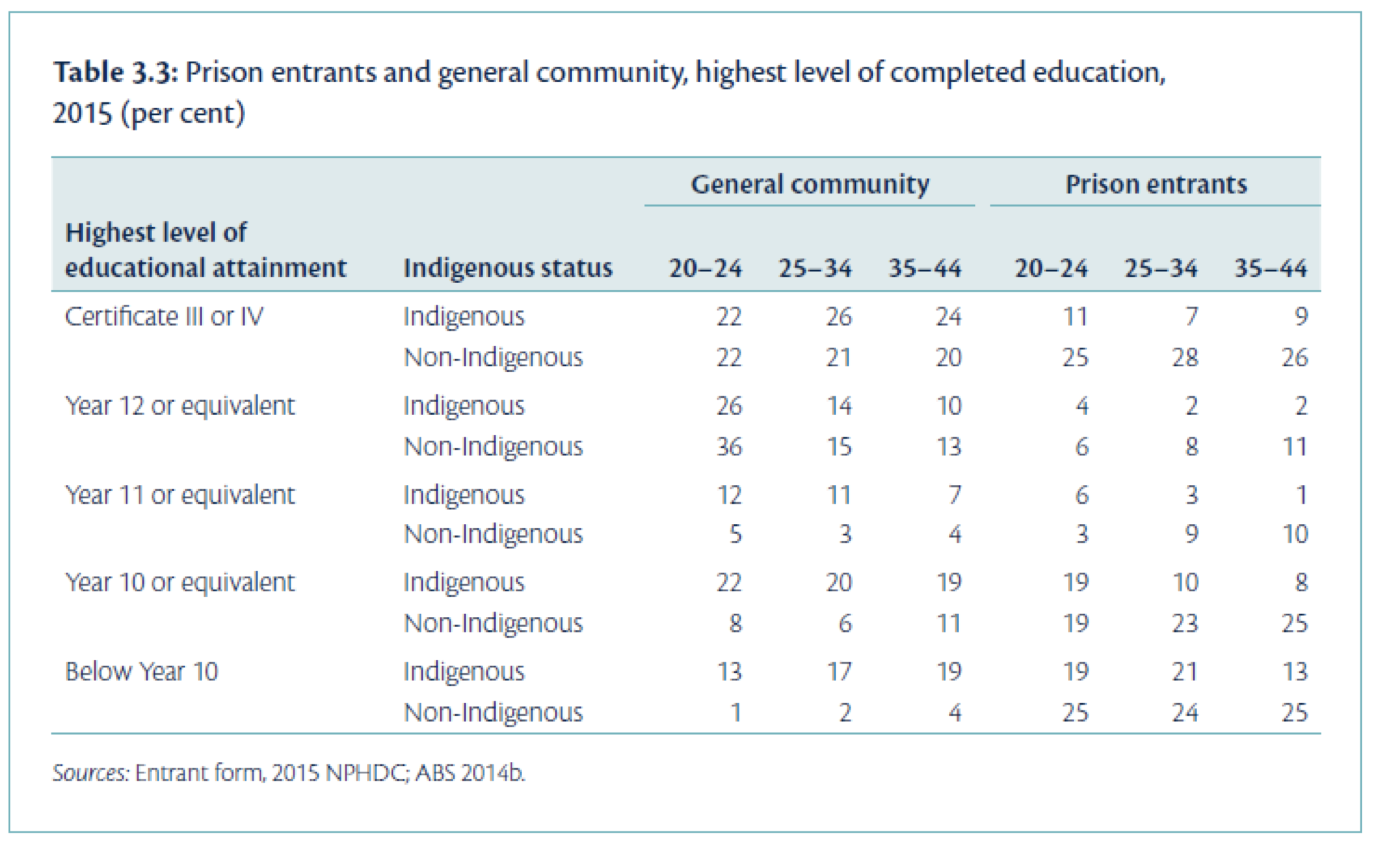
\includegraphics[width=0.66\linewidth,height=\textheight,keepaspectratio]{img/mod01/prisoner-education.png}

}

\caption{\label{fig-prison-education}Highest level of completed
education in prison entrants and the general community}

\end{figure}%

Source: Australian Institute of Health and Welfare 2015. The health of
Australia's prisoners 2015. Cat. no. PHE 207. Canberra: AIHW.

Some issues in this table:

\begin{itemize}
\tightlist
\item
  The title of the table does not contain full information about the
  variables in the table;
\item
  It is unclear how the percentages were calculated (which groupings
  added to 100\%);
\item
  The ages are not labelled as such, thus without reading the text in
  report it is unclear that these are age groupings.
\end{itemize}

\section{Summarising two categorical variables
graphically}\label{sec-two-catvar-graph}

Information from more than one variable can be presented as clustered or
multiple bar chart (bars side-by-side) (Figure~\ref{fig-bar-2}). This
type of graph is useful when examining changes in the categories
separately, but also comparing the grouping variable between the main
bar variable. Here we can see that Stage 3 and Stage 4 disease is the
most common for both males and females, but there are many more females
within each stage of disease.

\begin{figure}[H]

\centering{

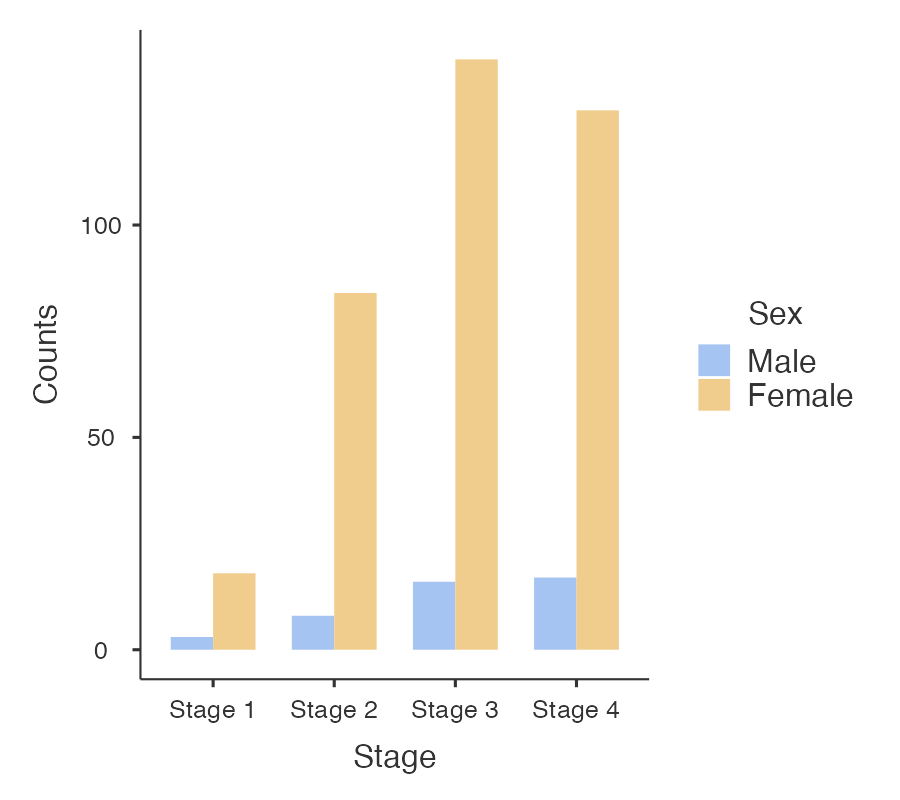
\includegraphics[width=0.75\linewidth,height=\textheight,keepaspectratio]{img/mod02/pbc-bar-stage-sex.png}

}

\caption{\label{fig-bar-2}Bar graph of stage of disease by sex from PBC
study}

\end{figure}%

An alternative bar graph is a stacked or composite bar graph, which
retains the overall height for each category, but differentiates the
bars by another variable (Figure~\ref{fig-bar-3}).

\begin{figure}[H]

\centering{

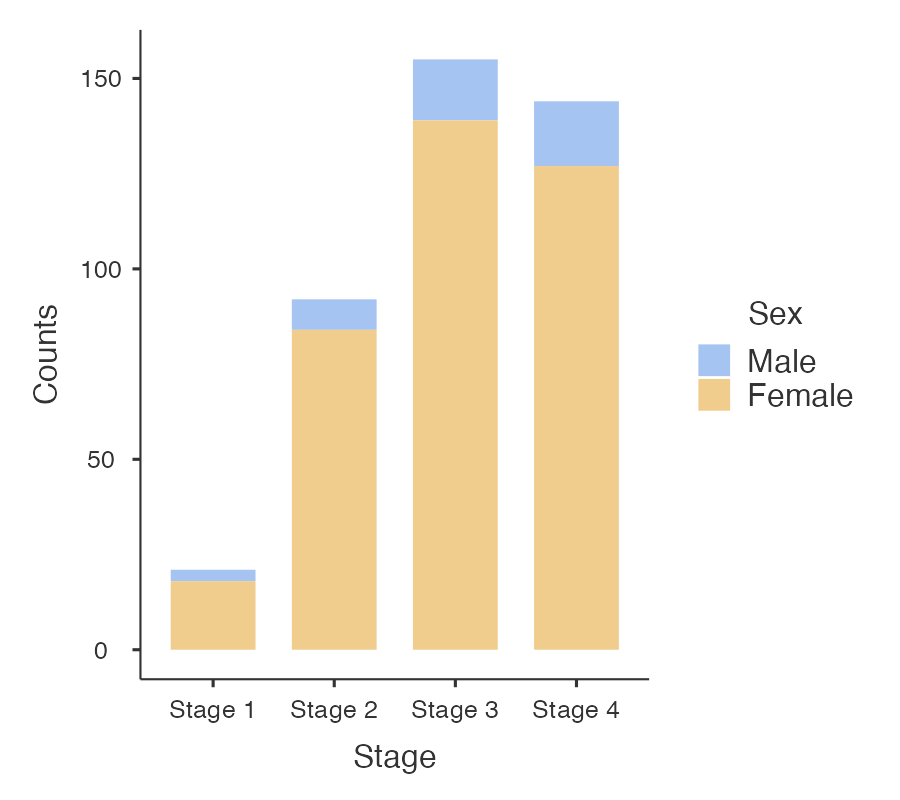
\includegraphics[width=0.75\linewidth,height=\textheight,keepaspectratio]{img/mod02/pbc-bar-stage-sex-stacked.png}

}

\caption{\label{fig-bar-3}Stacked bar graph of stage of disease by sex
from PBC study}

\end{figure}%

Finally, a stacked relative bar chart (Figure~\ref{fig-bar-4}) displays
the proportion of grouping variable for each bar, where each overall bar
represents 100\%. These graphs allow the reader to compare the
proportions between categories. We can easily see from
Figure~\ref{fig-bar-4} that the distribution of sex is similar across
each stage of disease.

\begin{figure}[H]

\centering{

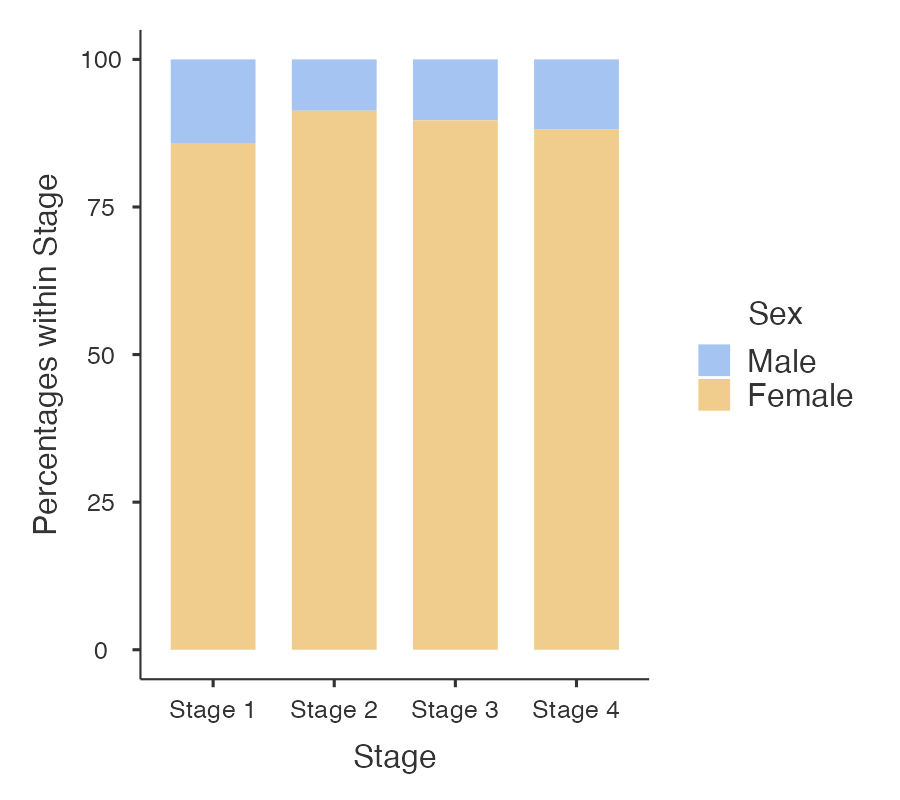
\includegraphics[width=0.75\linewidth,height=\textheight,keepaspectratio]{img/mod02/pbc-bar-stage-sex-stacked-relative.png}

}

\caption{\label{fig-bar-4}Relative frequency of sex within stage of
disease from PBC study}

\end{figure}%

\section{Presentation guidelines}\label{presentation-guidelines}

\subsection{Guidelines for presenting summary
statistics}\label{guidelines-for-presenting-summary-statistics}

When reporting summary statistics, it is important not to present
results with too many decimal places. Doing so implies that your data
have a higher level of precision than they do. For example, presenting a
mean blood pressure of 100.2487 mmHg implies that blood pressure can be
measured accurately to at least three decimal places.

There are a number of guidelines that have been written to help in the
presentation of numerical data. Many of these guidelines are based on
the number of decimal places, while others are based on the number of
significant figures. Briefly, the number of significant figures are
``the number of digits from the first non-zero digit to the last
meaningful digit, irrespective of the position of the decimal point.
Thus, 1.002, 10.02, 100200 (if this number is expressed to the nearest
100) all have four significant digits.'' Armitage et al. (2013)

A summary of these guidelines that will be used in this course appear in
Table~\ref{tbl-1-pres}.

\newpage{}

\begin{table}

\caption{\label{tbl-1-pres}Guidelines for presentation of statistical
results}

\centering{

\centering
\begin{talltblr}[         %% tabularray outer open
entry=none,label=none,
note{}={Sources: Altman (1990), Cole (2015), Assel et al. (2019)},
]                     %% tabularray outer close
{                     %% tabularray inner open
width={1\linewidth},
colspec={X[0.29]X[0.71]},
hline{2}={1-2}{solid, black, 0.05em},
hline{1}={1-2}{solid, black, 0.08em},
hline{17}={1-2}{solid, black, 0.08em},
}                     %% tabularray inner close
Summary statistic & Guideline (reference) \\
Mean & It is usually appropriate to quote the mean to one extra decimal place compared with the raw data. (Altman) \\
Median, Interquartile range, Range & As medians, interquartile ranges and ranges are based on individual data points, these values should be presented with the same precision as the original data. \\
Percentage & Percentages do not need to be given with more than one decimal place at most. When the sample size is less than 100, no decimal places should be given. (Altman) \\
Probability & It is acceptable to present probabilities to 2 or 3 decimal places. If the probability is presented as a percentage, present the percentage with 0 or 1 decimal place. \\
Standard deviation & The standard deviation should usually be given to the same accuracy as the mean, or with one extra decimal place. (Altman) \\
Standard error & As per standard deviation \\
Confidence interval & Use the same rule as for the corresponding effect size (be it mean, percentage, mean difference, regression coefficient, correlation coefficient or risk ratio) (Cole) \\
Test statistic & Test statistics should not be presented with more than two decimal places. \\
Degrees of freedom & Most degrees of freedom are whole numbers, and should be presented as such. If a test statistic has degrees of freedom with decimal places (the Welch t-statistic for example), present only one decimal place. \\
P-value & Report P-values to a single significant figure unless the P-value is close to 0.05 (say, 0.01 to 0.2), in which case, report two significant figures. Do not report `not significant` for P-values of 0.05 or higher. Very low P-values can be reported as P < 0.001 or P < 0.0001. A P-value can indeed be 1, although some investigators prefer to report this as >0.9. (Based on Assel) \\
Difference in means & As for the estimated means \\
Difference in proportions & As for the estimated proportions \\
Odds ratio / Relative risk & Hazard and odds ratios are normally reported to two decimal places, although this can be avoided for high odds ratios (Assel) \\
Correlation coefficient & One or two decimal places, or more when very close to ±1   (Cole) \\
Regression coefficient & Use one more significant figure than the underlying data   (adapted from Cole) \\
\end{talltblr}

}

\end{table}%

\subsection{Table presentation
guidelines}\label{table-presentation-guidelines}

Consider the following guidelines for the appropriate presentation of
tables in scientific journals and reports (Woodward, 2013).

\begin{enumerate}
\def\labelenumi{\arabic{enumi}.}
\tightlist
\item
  Each table (and figure) should be self-explanatory, i.e.~the reader
  should be able to understand it without reference to the text in the
  body of the report.

  \begin{itemize}
  \tightlist
  \item
    This can be achieved by using complete, meaningful labels for the
    rows and columns and giving a complete, meaningful title.
  \item
    Footnotes can be used to enhance the explanation.
  \end{itemize}
\item
  Units of the variables (and if needed, method of calculation or
  derivation) should be given and missing records should be noted
  (e.g.~in a footnote).
\item
  A table should be visually uncluttered.

  \begin{itemize}
  \tightlist
  \item
    Avoid use of vertical lines.
  \item
    Horizontal lines should not be used in every single row, but they
    can be used to group parts of the table.
  \item
    Sensible use of white space also helps enormously; use equal spacing
    except where large spaces are left to separate distinct parts of the
    table.
  \item
    Different typefaces (or fonts) may be used to provide
    discrimination, e.g.~use of bold type and/or italics.
  \end{itemize}
\item
  The rows and columns of each table should be arranged in a natural
  order to help interpretation. For instance, when rows are ordered by
  the size of the numbers they contain for a nominal variable, it is
  immediately obvious where relatively big and small contributions come
  from.
\item
  Tables should have a consistent appearance throughout the report so
  that the paper is easy to follow (and also for an aesthetic
  appearance). Conventions for labelling and ordering should be the same
  (for both tables as well as figures) for ease of comparison of
  different tables (and figures).
\item
  Consider if there is a particular table orientation that makes a table
  easier to read.
\end{enumerate}

Given the different possible formats of tables and their complexity,
some further guidelines are given in the following excellent references:

\begin{itemize}
\tightlist
\item
  Graphics and statistics for cardiology: designing effective tables for
  presentation and publication, Boers (2018)
\item
  Guidelines for Reporting of Figures and Tables for Clinical Research
  in Urology, Vickers et al. (2020)
\end{itemize}

\subsection{Graphical presentation
guidelines}\label{graphical-presentation-guidelines}

Consider the following guidelines for the appropriate presentation of
graphs in scientific journals and reports (Woodward, 2013).

\begin{itemize}
\tightlist
\item
  Figures should be self-explanatory and have consistent appearance
  through the report.
\item
  A title should give complete information. Note that figure titles are
  usually placed below the figure, whereas for tables titles are given
  above the table.
\item
  Axes should be labelled appropriately
\item
  Units of the variables should be given in the labelling of the axes.
  Use footnotes to indicate any calculation or derivation of variables
  and to indicate missing values
\item
  If the Y-axis has a natural origin, it should be included, or
  emphasised if it is not included.
\item
  If graphs are being compared, the Y-axis should be the same across the
  graphs to enable fair comparison
\item
  Columns of bar charts should be separated by a space
\item
  Three dimensional graphs should be avoided unless the third dimension
  adds additional information
\end{itemize}

\section{Probability}\label{probability}

Probability is defined as:

\begin{quote}
the chance of an event occurring, where an event is the result of an
observation or experiment, or the description of some potential outcome.
\end{quote}

Probabilities range from 0 (where the event will never occur) to 1
(where the event will always occur). For example, tossing a coin is an
experiment; one event is the coin landing with head up, while the other
event is the coin landing tails up. The set of all possible outcomes in
an experiment is called the sample space. For example, by tossing a coin
you can get either a head or a tail (called mutually exclusive events);
and by rolling a die you can get any of the six sides. Thus, for a die
the sampling space is: S = \{1, 2, 3, 4, 5, 6\}

With a fair (unbiased) die, the probability of each outcome occurring is
1/6 and its probability distribution is simply a probability of 1/6 for
each of the six numbers on a die.

\subsection{Additive law of
probability}\label{additive-law-of-probability}

How do we work out the probability that one roll of a die will turn out
to be a 3 or a 6? To do that, we first need to work out whether the
events (3 or 6 on the roll of a die) are mutually exclusive. Events are
mutually exclusive if they are events which cannot occur at the same
time. For example, rolling a die once and getting a 3 and 6 are mutually
exclusive events (you can roll one or the other but not both in a single
roll).

To obtain the probability of one or the other of two mutually exclusive
events occurring, the sum of the probabilities of each is taken. For
example, the probability of the roll of a die being a 3 or a 6 is the
sum of the probability of the die being 3 (i.e.~1/6) and the probability
of the die being 6 (also 1/6). With a fair die:

Probability of a die roll being 3 or 6 = \(1/6 + 1/6 = 1/3\)

Another way of putting it is:

P(die roll =3 or die roll =6) = P(die roll=3) + P(die roll=6) =
\(1/6 + 1/6 = 1/3\)

\subsubsection*{Example: Additive law for mutually exclusive
events}\label{example-additive-law-for-mutually-exclusive-events}
\addcontentsline{toc}{subsubsection}{Example: Additive law for mutually
exclusive events}

Consider that blood type can be organised into the ABO system (blood
types A, B, AB or O) An individual may only have one blood type.

Using the information from
https://www.donateblood.com.au/learn/about-blood let's consider the ABO
blood type system. The frequency distribution (prevalence) of the ABO
blood type system in the population represents the probability of each
of the outcomes. If we consider all possible blood type outcomes, then
the total of the probabilities will sum to 1 (100\%).

\begin{table}[h]

\caption{\label{tbl-2-1}Frequency of blood types}

\centering{

\centering
\begin{tblr}[         %% tabularray outer open
]                     %% tabularray outer close
{                     %% tabularray inner open
colspec={Q[]Q[]Q[]},
hline{2}={1-3}{solid, black, 0.05em},
hline{1}={1-3}{solid, black, 0.08em},
hline{7}={1-3}{solid, black, 0.08em},
}                     %% tabularray inner close
Blood Type & \% of population & Probability \\
A & 38\% & 0.38 \\
B & 10\% & 0.10 \\
AB & 3\% & 0.03 \\
O & 49\% & 0.49 \\
Total & 100\% & 1.00 \\
\end{tblr}

}

\end{table}%

In this example we consider: What is the probability that an individual
will have either blood group O or A?

Since blood type is mutually exclusive, the probability that either one
or the other occurs is the sum of the individual probabilities. These
are mutually exclusive events so we can say P(O or A) = P(O) + P(A)

Thus, the answer is: P(Blood type O) + P(Blood type A) = 0.49 + 0.38 =
0.87

\subsection{Multiplicative law of
probability}\label{multiplicative-law-of-probability}

The additive law of probability lets us consider the probability of
different outcomes in a single experiment. The multiplicative law lets
us consider the probability of multiple events occurring in a particular
order. For example: if I roll a die twice, what is the probability of
rolling a 3 and \emph{then} a 6?

These events are independent: the probability of rolling a 6 on the
second roll is not affected by the first roll.

The multiplicative law of probability states:

\begin{quote}
If A and B are independent, then P(A and B) = P(A) \(\times\) P(B).
\end{quote}

So, the probability of rolling a 3 and then a 6 is: P(3 and 6) =
\(1/6 \times 1/6 = 1/36\).

Note here that the order matters -- we are considering the probability
of rolling a 3 and then a 6, not the probability of rolling a 6 and then
a 3.

\section{Probability distributions}\label{probability-distributions}

\begin{quote}
A probability distribution is a table or a function that provides the
probabilities of all possible outcomes for a random event.
\end{quote}

For example, the probability distribution for a single coin toss is
straightforward: the probability of obtaining a head is 0.5, and the
probability of obtaining a tail is 0.5, and this can be summarised in
Table~\ref{tbl-coin}.

\begin{table}[h]

\caption{\label{tbl-coin}Probability distribution for a single coin
toss}

\centering{

\centering
\begin{tblr}[         %% tabularray outer open
]                     %% tabularray outer close
{                     %% tabularray inner open
colspec={Q[]Q[]},
hline{2}={1-2}{solid, black, 0.05em},
hline{1}={1-2}{solid, black, 0.08em},
hline{4}={1-2}{solid, black, 0.08em},
}                     %% tabularray inner close
Coin face & Probability \\
Heads & 0.5 \\
Tails & 0.5 \\
\end{tblr}

}

\end{table}%

Similarly, the probability distribution for a single roll of a die is
straightforward: each face has a probability of 1/6
(Table~\ref{tbl-die}).

\begin{table}[h]

\caption{\label{tbl-die}Probability distributions for a single roll of a
die}

\centering{

\centering
\begin{tblr}[         %% tabularray outer open
]                     %% tabularray outer close
{                     %% tabularray inner open
colspec={Q[]Q[]},
hline{2}={1-2}{solid, black, 0.05em},
hline{1}={1-2}{solid, black, 0.08em},
hline{8}={1-2}{solid, black, 0.08em},
}                     %% tabularray inner close
Face of a die & Probability \\
1 & 1/6 \\
2 & 1/6 \\
3 & 1/6 \\
4 & 1/6 \\
5 & 1/6 \\
6 & 1/6 \\
\end{tblr}

}

\end{table}%

Things become more complicated when we consider multiple coin-tosses, or
rolls of a die. These series of events can be summarised by considering
the number of times a certain outcome is observed. For example, the
probability of obtaining three heads from five coin tosses.

Probability distributions can be used in two main ways:

\begin{enumerate}
\def\labelenumi{\arabic{enumi}.}
\tightlist
\item
  To calculate the probability of an event occurring. This seems trivial
  for the coin-toss and die-roll examples above. However, we can
  consider more complex events, as below.
\item
  To understand the behaviour of a sample statistic. We will see in
  Modules 3 and 4 that we can assume the mean of a sample follows a
  probability distribution. We can obtain useful information about the
  sample mean by using properties of the probability distribution.
\end{enumerate}

\section{Discrete random variables and their probability
distributions}\label{discrete-random-variables-and-their-probability-distributions}

Rather than thinking of random events, we often use the term
\emph{random variable} to describe a quantity that can have different
values determined by chance.

A \emph{discrete random variable} is a random variable that can take on
only countable values (that is, non-negative whole numbers). An example
of a discrete random variable is the number of heads observed in a
series of coin tosses.

A discrete random variable can be summarised by listing all the possible
values that the variable can take. As defined earlier, a table, formula
or graph that presents these possible values, and their associated
probabilities, is called a probability distribution.

Example: let's consider the number of heads in a series of three coin
tosses. We might observe 0 heads, or 1 head, or 2, or 3 heads. If we let
X denote the number of heads in a series of three coin tosses, then
possible values of X are 0, 1, 2 or 3.

We write the probability of observing x heads as P(X=x). So P(X=0) is
the probability that the three tosses has no heads. Similarly, P(X=1) is
the probability of observing one head.

The possible combinations for three coin tosses are as follows:

\begin{table}[h]

\caption{\label{tbl-2-3toss}The number of heads from three coin tosses}

\centering{

\centering
\begin{tblr}[         %% tabularray outer open
]                     %% tabularray outer close
{                     %% tabularray inner open
colspec={Q[]Q[]},
hline{2}={1-2}{solid, black, 0.05em},
hline{1}={1-2}{solid, black, 0.08em},
hline{10}={1-2}{solid, black, 0.08em},
hline{3}={1-2}{solid, black, 0.1em},
hline{6}={1-2}{solid, black, 0.1em},
hline{9}={1-2}{solid, black, 0.1em},
}                     %% tabularray inner close
Pattern & Number of heads \\
Tail, Tail, Tail & 0 \\
Head, Tail, Tail &   \\
Tail, Head, Tail & 1 \\
Tail, Tail, Head &   \\
Head, Head, Tail &   \\
Head, Tail, Head & 2 \\
Tail, Head, Head &   \\
Head, Head, Head & 3 \\
\end{tblr}

}

\end{table}%

There are eight possible outcomes from three coin tosses (permutations).
If we assume an equal chance of observing a head or a tail, each
permutation above is equally likely, and so has a probability of 1/8.

If we consider the possibility of observing just one head out of the
three tosses, this can happen in three ways (HTT, THT, TTH). So the
probability of observing one head is calculated using the additive law:
P(X=1) = \(\tfrac{1}{8} + \tfrac{1}{8} + \tfrac{1}{8} = \tfrac{3}{8}\).

Therefore, the probability distribution for X, the number of heads from
three coin tosses, is as follows:

\begin{table}[h]

\caption{\label{tbl-2-4}Probability distribution for the number of heads
from three coin tosses}

\centering{

\centering
\begin{tblr}[         %% tabularray outer open
]                     %% tabularray outer close
{                     %% tabularray inner open
colspec={Q[]Q[]},
hline{2}={1-2}{solid, black, 0.05em},
hline{1}={1-2}{solid, black, 0.08em},
hline{6}={1-2}{solid, black, 0.08em},
}                     %% tabularray inner close
x (number of heads observed) & P(X=x) \\
0 & 1/8 \\
1 & 1/8 + 1/8 + 1/8 = 3/8 \\
2 & 1/8 + 1/8 + 1/8 = 3/8 \\
3 & 1/8 \\
\end{tblr}

}

\end{table}%

Note that the probabilities sum to 1.

The above example was based on a coin toss, where flipping a head or a
tail is equally likely (both have probabilities of 0.5). Let's consider
a case where the probability of an event is not equal to 0.5: having
blood type A.

From Table~\ref{tbl-2-1}, the probability that a person has Type A blood
is 0.38, and therefore, the probability that a person does not have Type
A blood is 0.62 (1--0.38). If we considered taking a random sample of
three people, the probability that all three would have Type A blood is
0.38 × 0.38 × 0.38 (using the multiplicative rule above) -- and there is
only one way this could happen.

The number of ways two people out of three could have Type A blood is 3,
and each permutation is listed in Table~\ref{tbl-2-5}. The probability
of observing each of the three patterns is the same, and can be
calculated using the multiplicative rule: 0.38 × 0.38 × 0.62 = 0.0895.

\begin{table}[h]

\caption{\label{tbl-2-5}Combinations and probabilities of Type A blood
in three people}

\centering{

\centering
\begin{tblr}[         %% tabularray outer open
]                     %% tabularray outer close
{                     %% tabularray inner open
colspec={Q[]Q[]Q[]Q[]},
hline{2}={1-4}{solid, black, 0.05em},
hline{1}={1-4}{solid, black, 0.08em},
hline{10}={1-4}{solid, black, 0.08em},
hline{3}={1-4}{solid, black, 0.1em},
hline{6}={1-4}{solid, black, 0.1em},
hline{9}={1-4}{solid, black, 0.1em},
}                     %% tabularray inner close
Person 1 & Person 2 & Person 3 & Probability \\
A & A & A & 0.38 × 0.38 × 0.38 = 0.0549 \\
A & A & Not A & 0.38 × 0.38 × 0.62 = 0.0895 \\
A & Not A & A & 0.38 × 0.62 × 0.38 = 0.0895 \\
Not A & A & A & 0.62 × 0.38 × 0.38 = 0.0895 \\
A & Not A & Not A & 0.38 × 0.62 × 0.62 = 0.1461 \\
Not A & A & Not A & 0.62 × 0.38 × 0.62 = 0.1461 \\
Not A & Not A & A & 0.62 × 0.62 × 0.38 = 0.1461 \\
Not A & Not A & Not A & 0.62 × 0.62 × 0.62 = 0.2383 \\
\end{tblr}

}

\end{table}%

Table~\ref{tbl-2-6} gives the probability of each of the blood type
combinations we could observe in three people. The probability of
observing a certain number of people (say, k) with Type A blood from a
sample of three people can be calculated by summing the combinations:

\begin{table}[h]

\caption{\label{tbl-2-6}Probabilities of observing numbers of people
with Type A blood in a sample of three people}

\centering{

\centering
\begin{tblr}[         %% tabularray outer open
]                     %% tabularray outer close
{                     %% tabularray inner open
colspec={Q[]Q[]},
hline{2}={1-2}{solid, black, 0.05em},
hline{1}={1-2}{solid, black, 0.08em},
hline{6}={1-2}{solid, black, 0.08em},
}                     %% tabularray inner close
Number of people with Type A blood & Probability of each pattern \\
3 & 0.0549 \\
2 & 0.0895 + 0.0895 + 0.0895 = 0.2689 \\
1 & 0.1461 + 0.1461 + 0.1461 = 0.4382 \\
0 & 0.2383 \\
\end{tblr}

}

\end{table}%

\section{Binomial distribution}\label{binomial-distribution}

The above are examples of the binomial distribution. The binomial
distribution is used when we have a collection of random events, where
each random event is binary (e.g.~Heads vs Tails, Type A blood vs Not
Type A blood, Infected vs Not infected). The binomial distribution
calculates (in general terms):

\begin{itemize}
\tightlist
\item
  the probability of observing k successes
\item
  from a collection of n trials
\item
  where the probability of a success in one trial is p.
\end{itemize}

The terms used here can be defined as:

\begin{itemize}
\tightlist
\item
  a success is simply an event of interest from a binary random event.
  In the coin-toss example, ``success'' was tossing a Head. In the blood
  type example, we were only interested in whether someone was Type A or
  not Type A, so ``success'' was a blood of Type A. We tend to use the
  word ``success'' to mean ``an event of interest'', and ``failure'' as
  ``an event not of interest''.
\item
  the number of trials refers to the number of random events observed.
  In both examples, we observed three events (three coin tosses, three
  people).
\item
  the probability of a success (p) simply refers to the probability of
  the event of interest. In the coin toss example, this was the
  probability of tossing a Heads (=0.5); for the blood-type example,
  this was the probability of having Type A blood (0.38).
\end{itemize}

Putting all this together, we say that we have a binomial experiment. To
satisfy the assumptions of a binomial distribution, our experiment must
satisfy the following criteria:

\begin{enumerate}
\def\labelenumi{\arabic{enumi}.}
\tightlist
\item
  The experiment consists of fixed number (n) of trials.
\item
  The result of each trial falls into only one of two categories -- the
  event occurred (``success'') or the event did not occur (``failure'').
\item
  The probability, p, of the event occurring remains constant for each
  trial.
\item
  Each trial of the experiment is independent of the other trials.
\end{enumerate}

We have shown in the examples above how we can calculate the
probabilities for small experiments (n=3). Once n becomes large,
constructing such probability distribution tables becomes difficult. The
general formula for calculating the probability of observing k successes
from n trials, where each trial has a probability of success of p is
given by:

\[ P(X=k) = \frac{n!}{k! (n-k)!} \times p^k \times (1-p)^{n-k} \]

where
\(n! = n \times (n-1) \times (n-2) \times \dots \times 2 \times 1\).

\textbf{Note that this formula is almost never calculated by hand.}
Instructions for calculating binomial probabilities are given in the
jamovi and R notes at the end of this Module.

\subsubsection*{Worked example}\label{worked-example}
\addcontentsline{toc}{subsubsection}{Worked example}

A population-based survey conducted by the AIHW (2008) of a random
sample of the Australian population estimated that in 2007, 19.8\% of
the Australian population were current smokers.

\begin{enumerate}
\def\labelenumi{\alph{enumi})}
\tightlist
\item
  From a random sample of 6 people from the Australian population in
  2007, what is the probability that 3 of them will be smokers?
\item
  What is the probability that among the six persons, at least 4 will be
  smokers?
\item
  What is the probability that at most, 2 will be smokers?
\end{enumerate}

\subsubsection*{Solution}\label{solution}
\addcontentsline{toc}{subsubsection}{Solution}

\begin{enumerate}
\def\labelenumi{\alph{enumi})}
\tightlist
\item
  Calculating this single binomial probability is best done using
  software.
\end{enumerate}

We can use the \href{https://mabognar.github.io/apps/bin.html}{applet}
to calculate this, or use the \texttt{dbinom} function in R with x=3,
size=6, and prob=0.198. This gives an answer of 0.08.

\begin{enumerate}
\def\labelenumi{\alph{enumi})}
\setcounter{enumi}{1}
\tightlist
\item
  In common language, getting ``at least 4'' smokers means getting 4, 5
  or 6 smokers. Since these are mutually exclusive events, we can apply
  the additive law to find the probability of getting at least 4
  smokers:
\end{enumerate}

\[ P(X \ge 4) = P(X=4) + P(X=5) + P(X=6) \] Using the same binomial
probability functions as in the previous question, we could calculate

\begin{itemize}
\tightlist
\item
  P(X=4) = 0.0148
\item
  P(X=5) = 0.00146
\item
  P(X=6) = 0.0000603
\end{itemize}

Answer: \(P(X \ge 4) = 0.0148 + 0.00146 + 0.0000603 = 0.016\)

We can use the \href{https://mabognar.github.io/apps/bin.html}{applet}
to calculate this, or in R we can use the \texttt{pbinom} function with
the \texttt{lower.tail=FALSE} option.

\begin{enumerate}
\def\labelenumi{\alph{enumi})}
\setcounter{enumi}{2}
\tightlist
\item
  Observing at most two means observing 0, 1 or 2 smokers. Therefore,
  the probability of observing at most 2 smokers is:
\end{enumerate}

\begin{itemize}
\tightlist
\item
  P(X \(\le\) 2) = P(X=0) + P(X=1) + P(X=2)
\item
  P(X=0) = 0.266
\item
  P(X=1) = 0.394
\item
  P(X=2) = 0.243
\end{itemize}

Answer: P(X \(\le\) 2) = 0.266+0.394+0.243=0.903

Again, we can use the
\href{https://mabognar.github.io/apps/bin.html}{applet} to calculate
this, or use the \texttt{pbinom} function in R.

\newpage{}

\bookmarksetup{startatroot}

\chapter*{jamovi notes}\label{jamovi-notes}
\addcontentsline{toc}{chapter}{jamovi notes}

\markboth{jamovi notes}{jamovi notes}

\section{Producing a one-way frequency
table}\label{producing-a-one-way-frequency-table}

The simplest way to summarise categorical variables is with a one-way
frequency table. These are constructed using \textbf{Analyses
\textgreater{} Exploration}. We will illustrate this by summarising the
variable \texttt{sex} from the \texttt{pbc.rds} data from the previous
module.

\pandocbounded{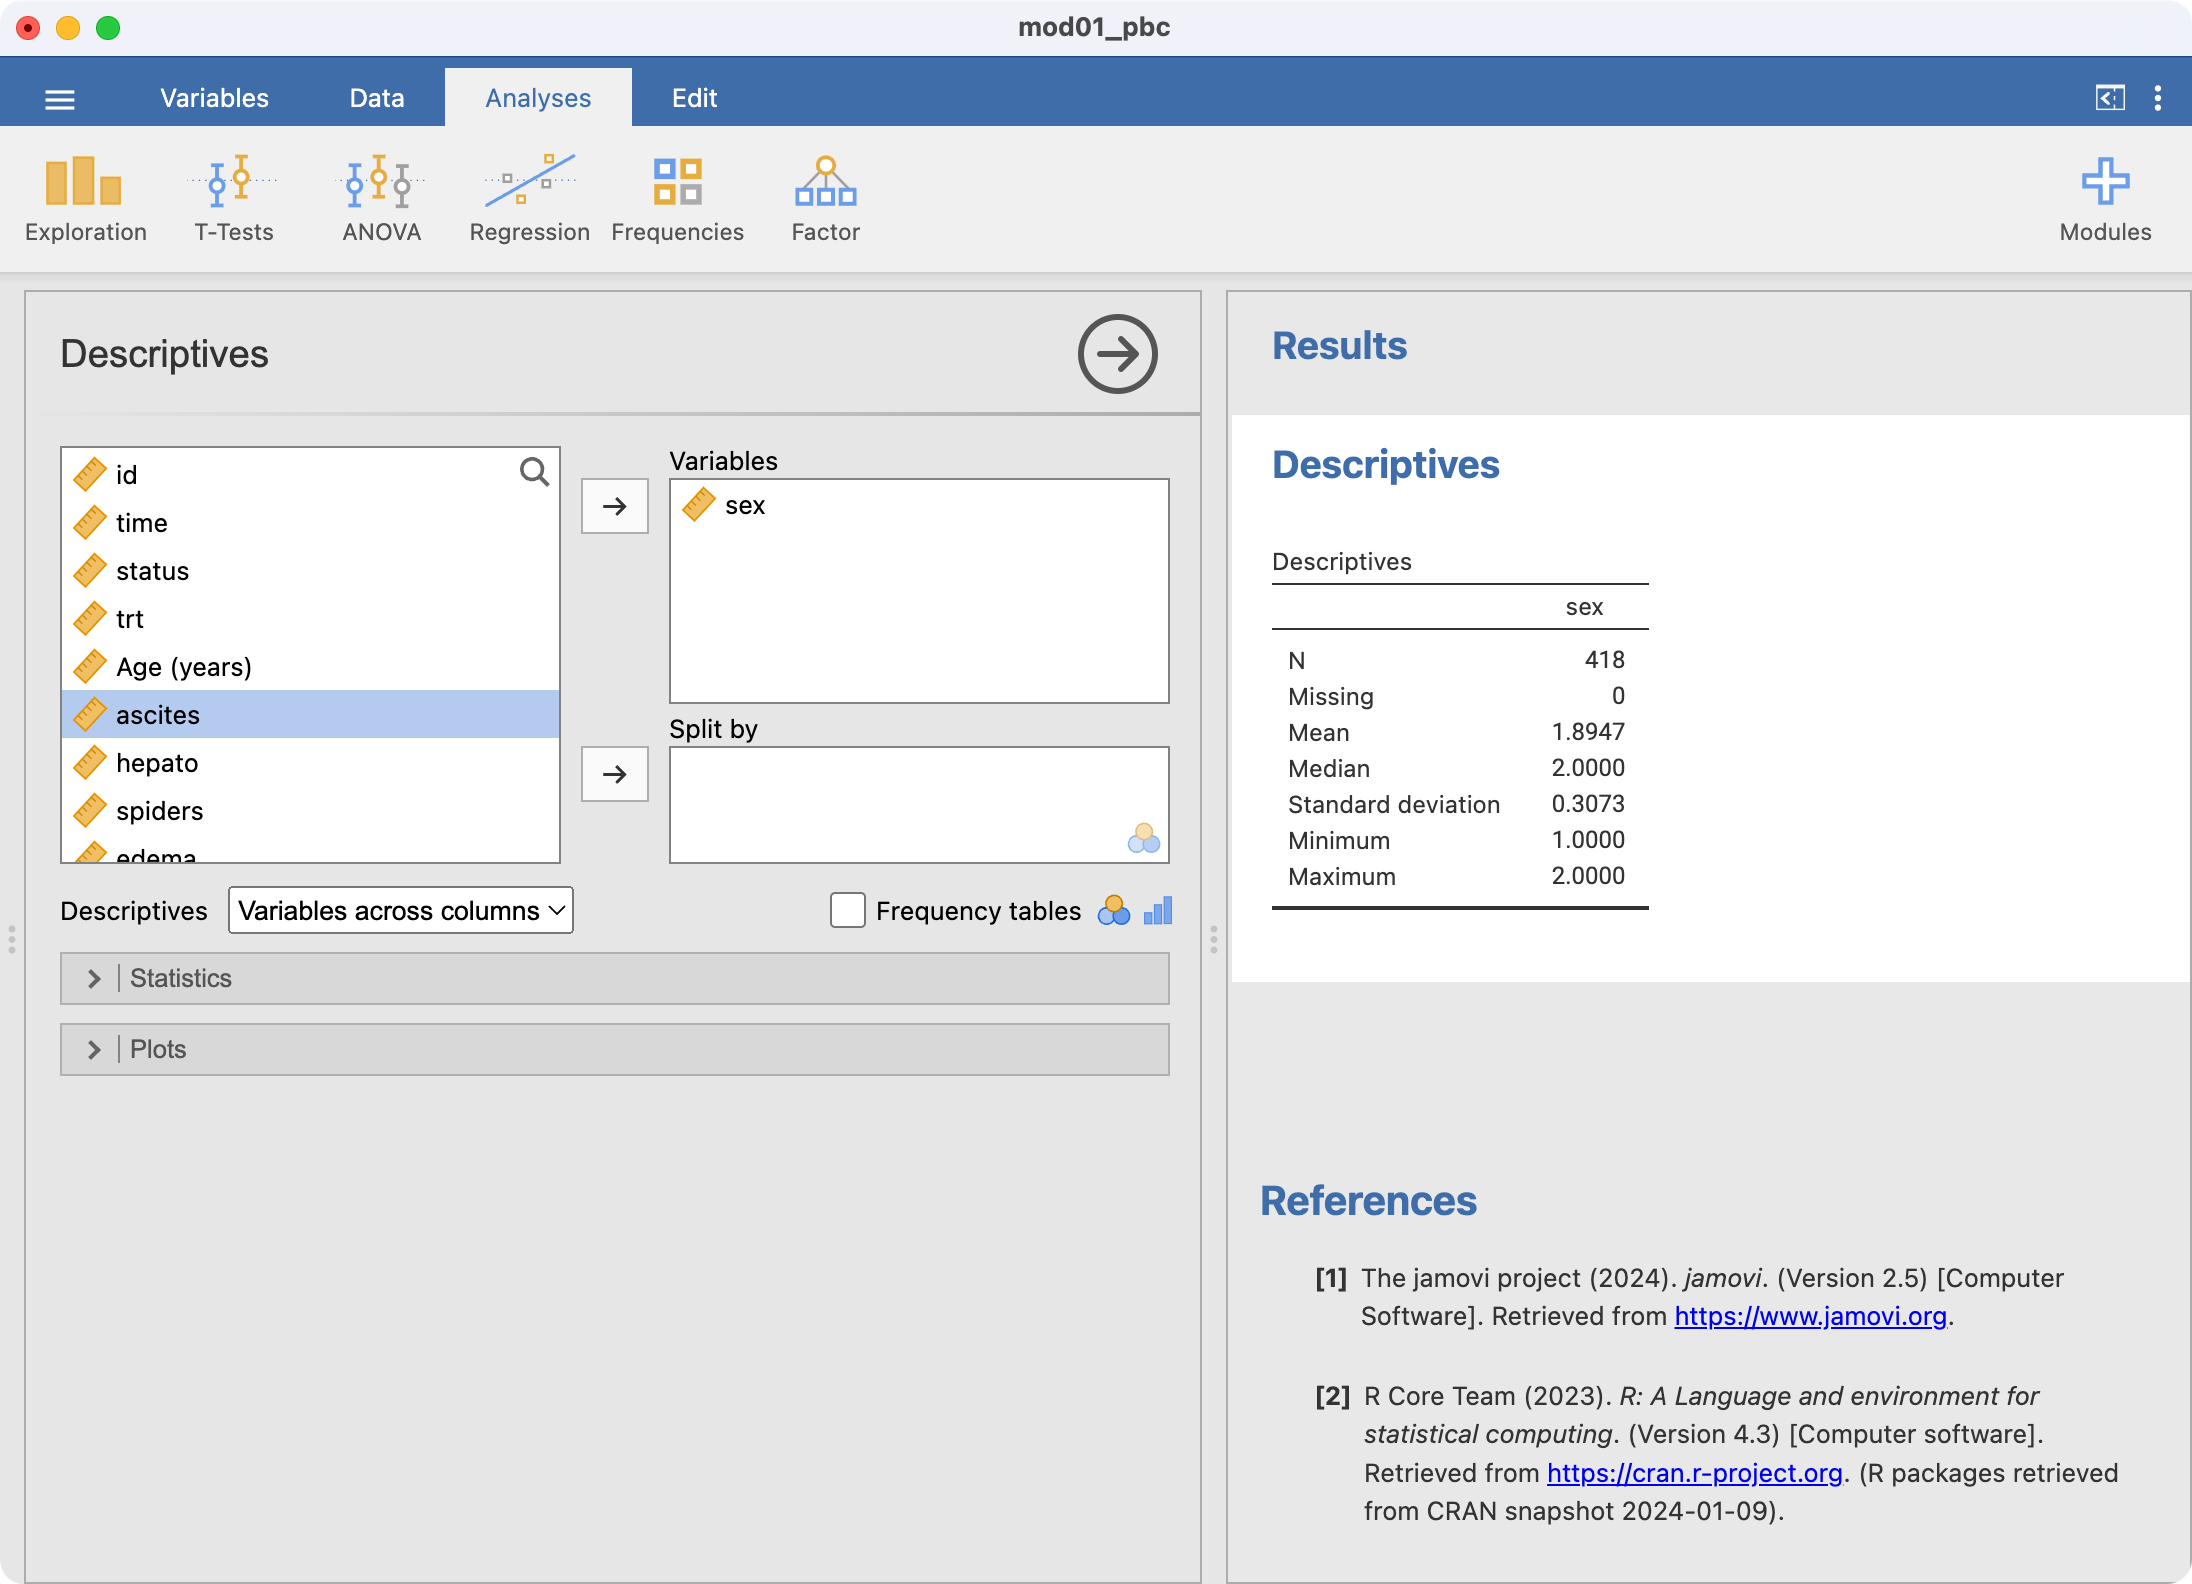
\includegraphics[keepaspectratio]{img/mod02/jamovi/mod02-onefreq01.png}}

jamovi has summarised \texttt{sex} here, just as we asked it to, however
it has analysed \texttt{sex} as if it was a continuous variable. This is
incorrect: \texttt{sex} is a categorical variable. This can be corrected
by defining \texttt{sex} to be categorical within \textbf{Data
\textgreater{} Setup}:

\begin{enumerate}
\def\labelenumi{\arabic{enumi}.}
\tightlist
\item
  Select \texttt{sex}, then choose \textbf{Nominal} as the Measure type.
  jamovi now lists the levels of \texttt{sex} as 1 and 2. These should
  be replaced by the categories they represent.
\item
  From the \texttt{mod01\_pbc\_info.txt} file, we see that 1 represents
  Male, and 2 represents Female. These labels can be added by typing in
  the appropriate cell. The completed screen should look like this:
\end{enumerate}

\pandocbounded{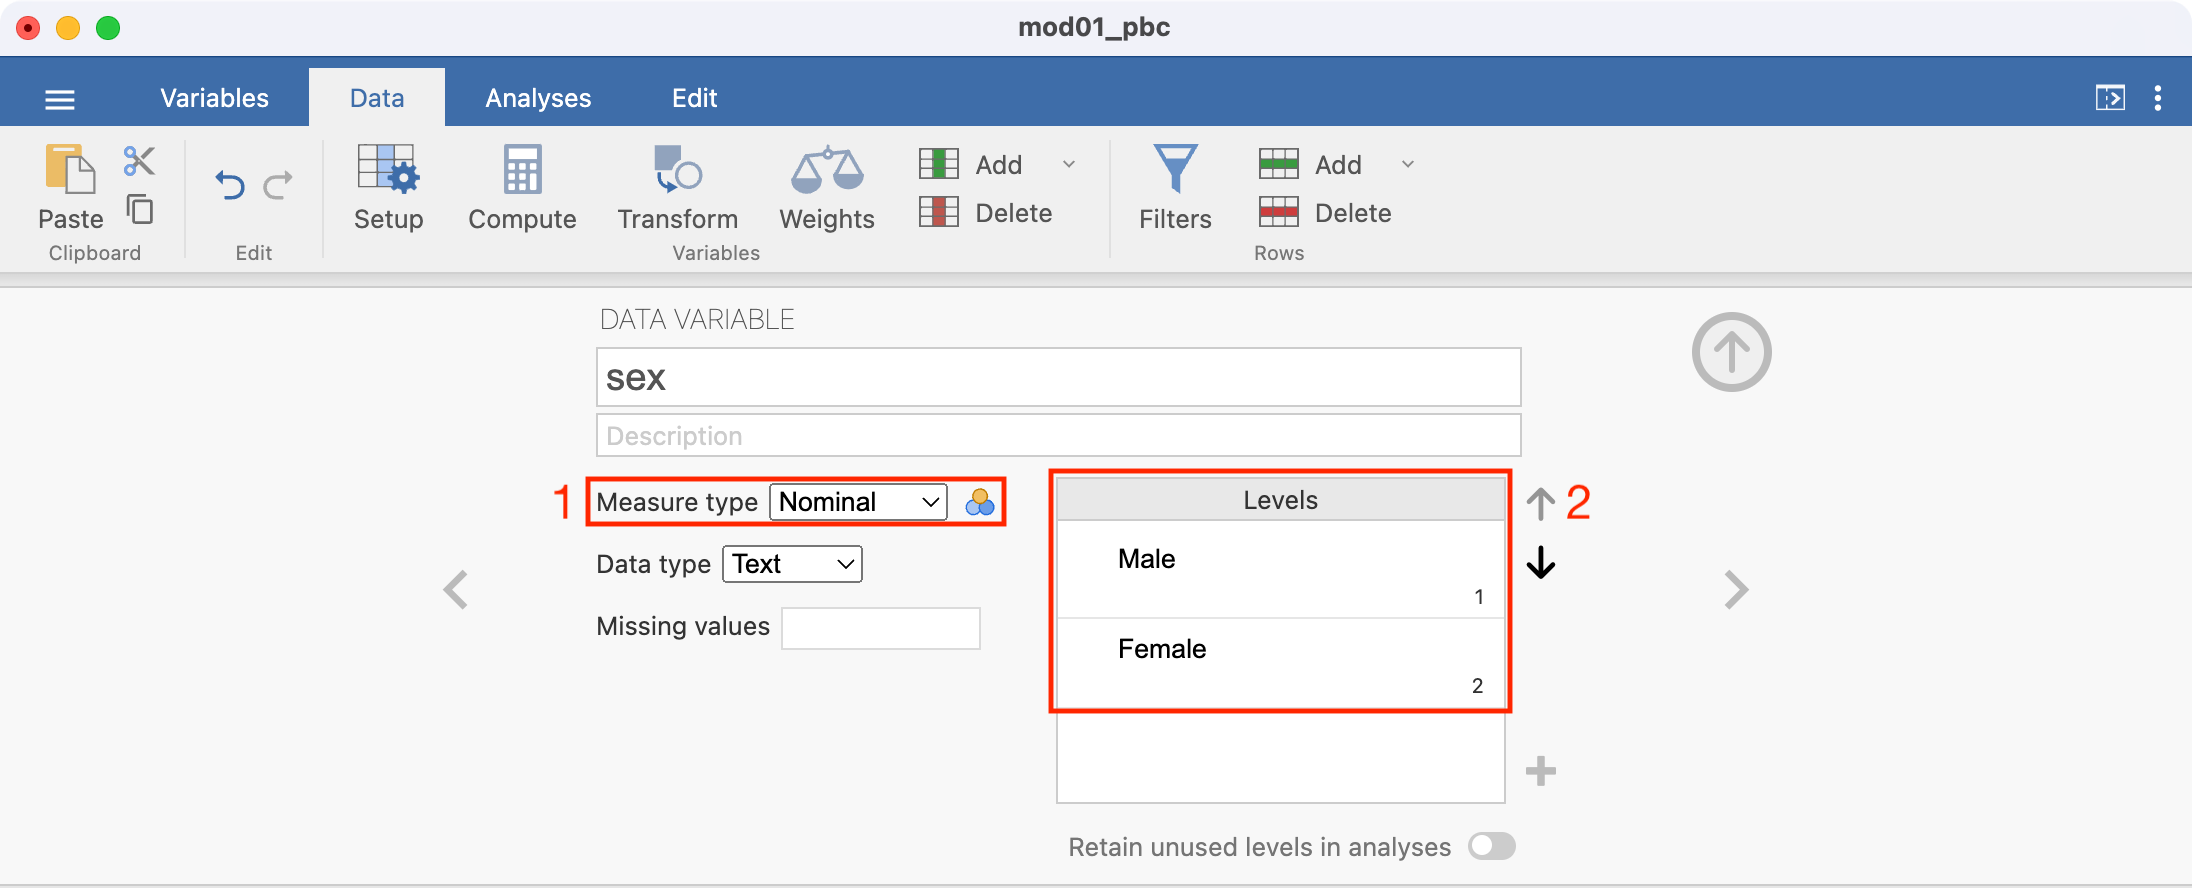
\includegraphics[keepaspectratio]{img/mod02/jamovi/mod02-onefreq02.png}}

Clicking back to the original summary of sex shows that jamovi is no
longer treating \texttt{sex} as a continuous variable, but there is
little output in the summary:

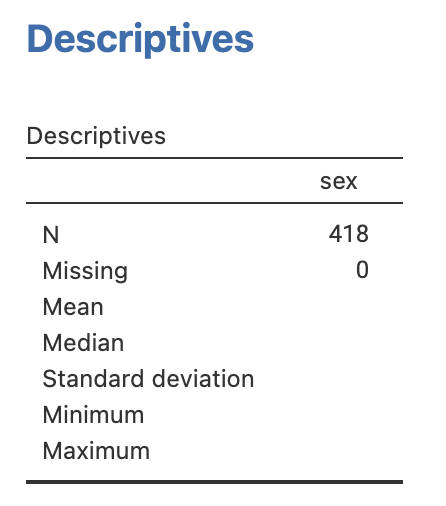
\includegraphics[width=0.3\linewidth,height=\textheight,keepaspectratio]{img/mod02/jamovi/mod02-onefreq03.png}

Click \textbf{Frequency tables} in the main Descriptives window to
request the one-way frequency table:

\pandocbounded{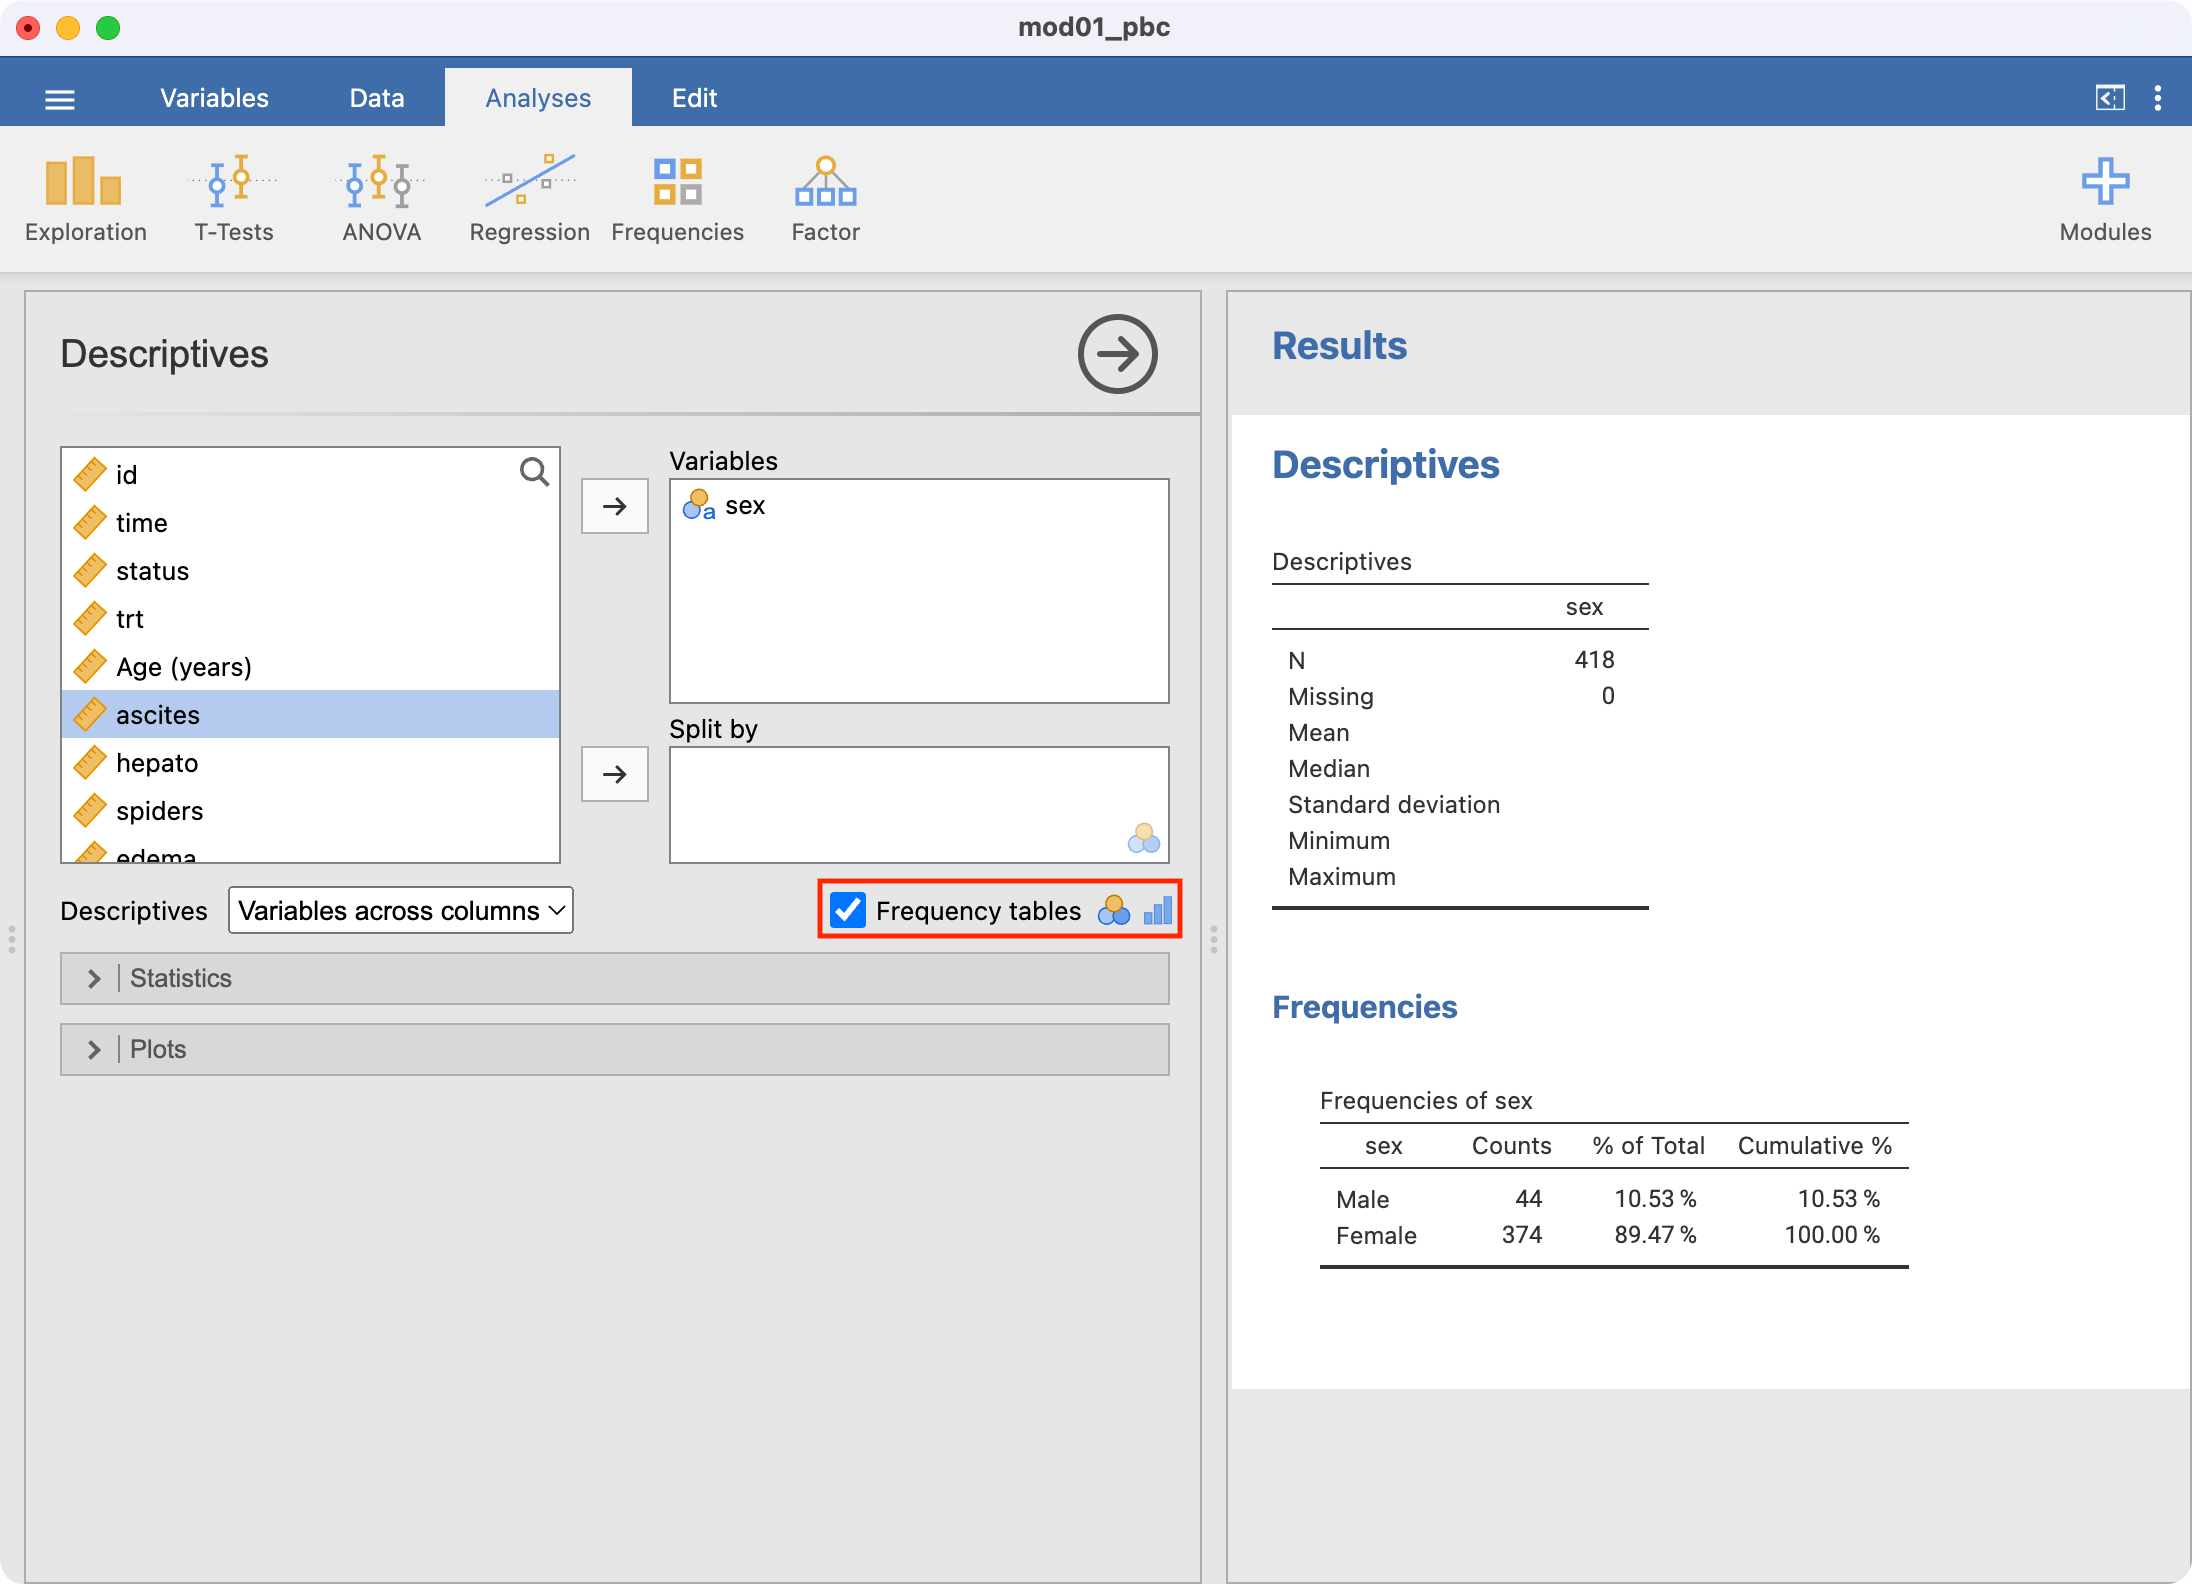
\includegraphics[keepaspectratio]{img/mod02/jamovi/mod02-onefreq04.png}}

\section{Producing a two-way frequency
table}\label{producing-a-two-way-frequency-table}

Two-way tables are constructed using \textbf{Analyses \textgreater{}
Frequencies \textgreater{} Contingency Tables \textgreater{} Independent
Samples}. Note that \textbf{both variables must be defined as Nominal or
Ordinal variables}. As an example, to produce a two-way table of disease
stage by sex:

\pandocbounded{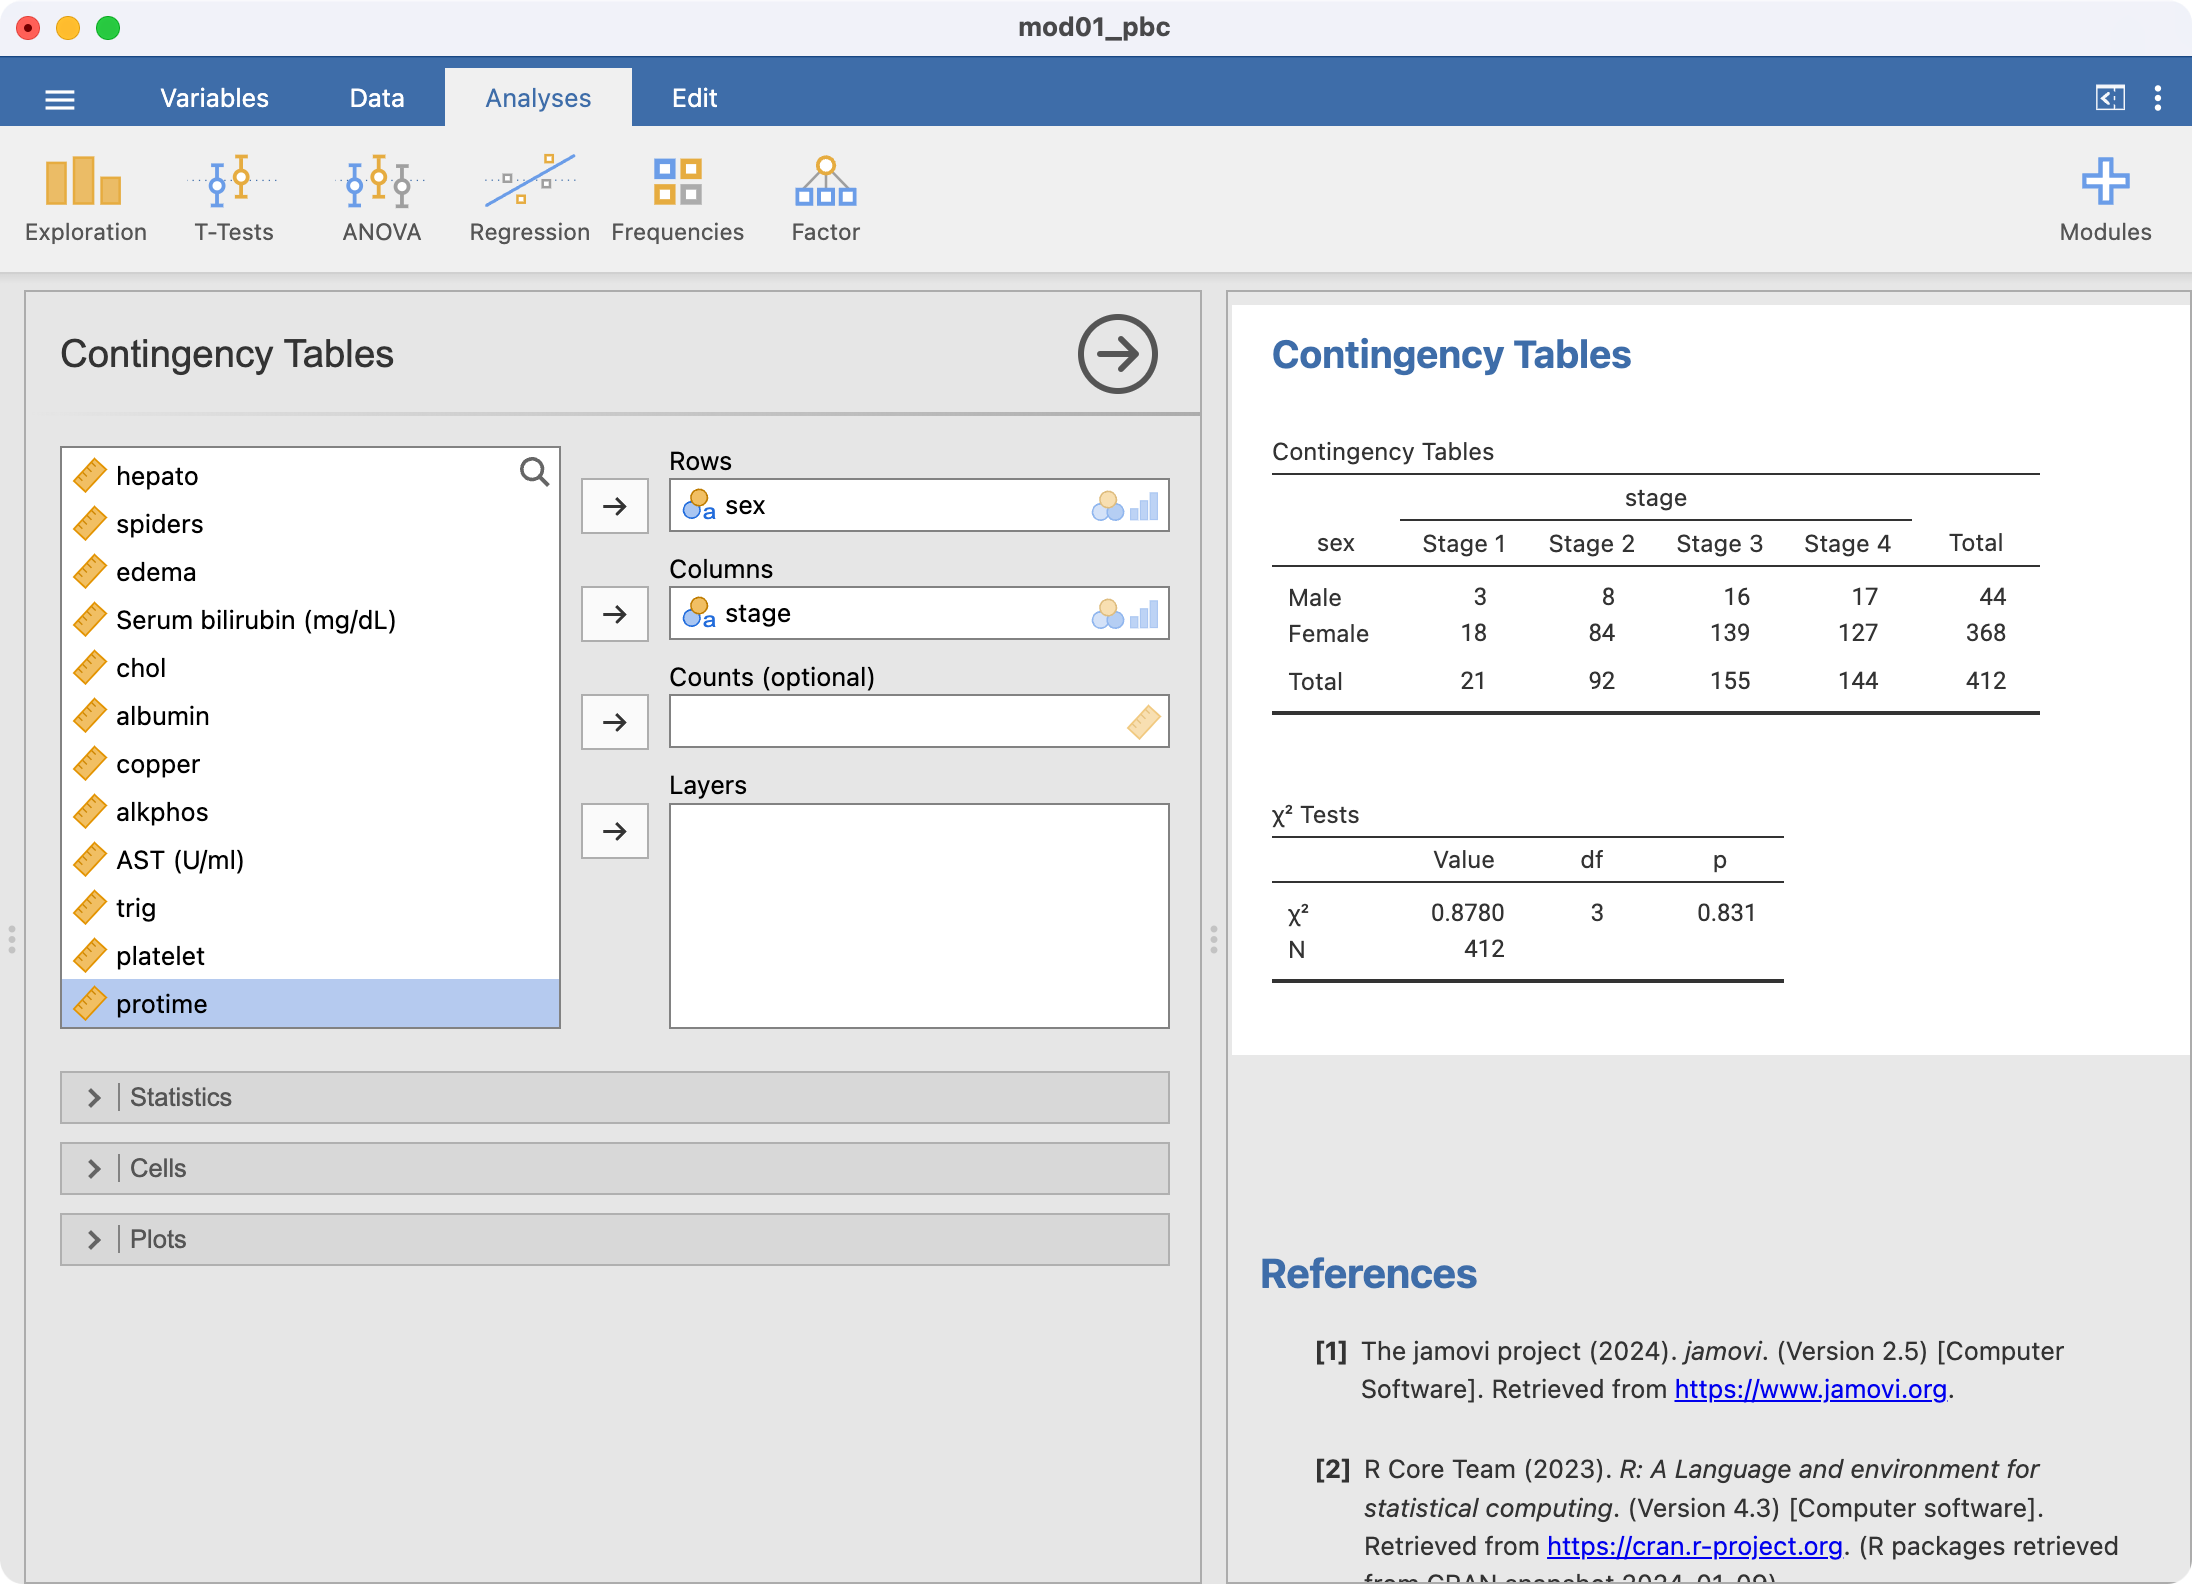
\includegraphics[keepaspectratio]{img/mod02/jamovi/mod02-twofreq01.png}}

\textbf{Ignore the output labelled χ\textsuperscript{2} tests for now.}

Row or column percents can be requested in the \textbf{Cells} section.
For example, to calculate the proportion of males within each stage of
disease, we would request column percents:

\pandocbounded{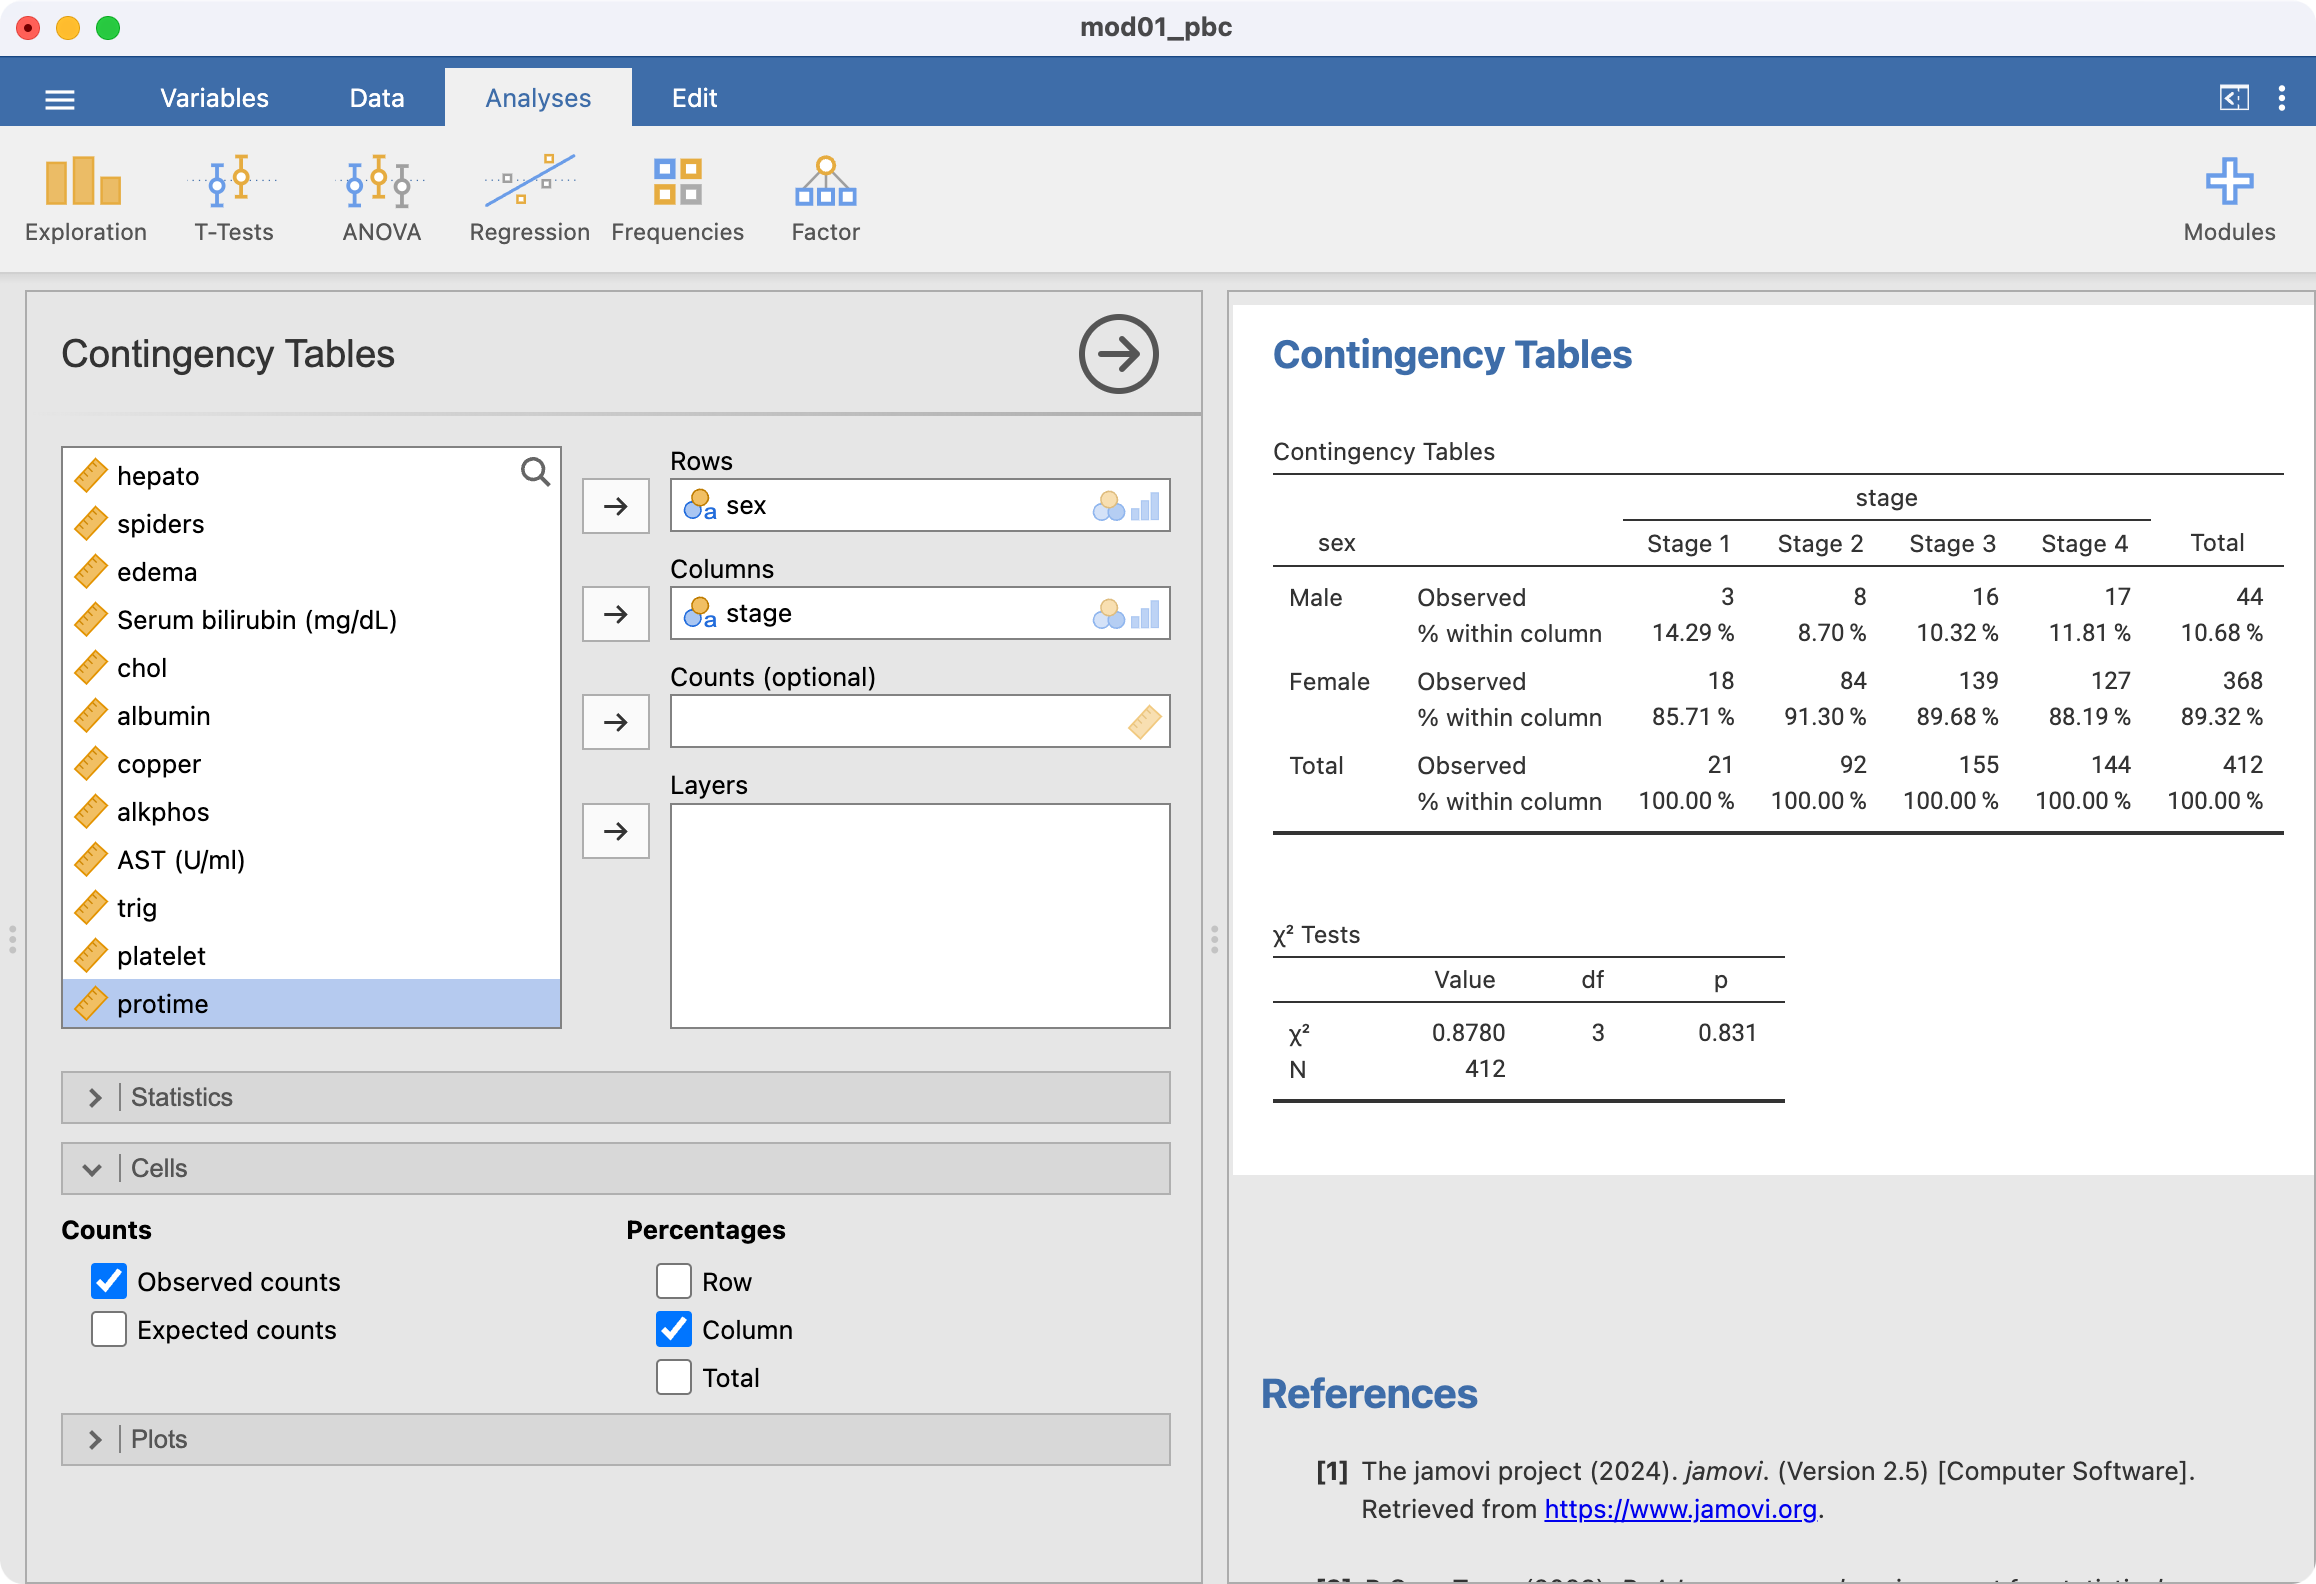
\includegraphics[keepaspectratio]{img/mod02/jamovi/mod02-twofreq02.png}}

\section{Creating bar charts for one categorical
variable}\label{creating-bar-charts-for-one-categorical-variable}

Here we will create the bar chart shown in Figure~\ref{fig-bar-1} using
the \texttt{mod01\_pbc.rds} dataset. The x-axis of this graph will be
the stage of disease, and the y-axis will show the number of
participants in each category.

Bar charts are created in the \textbf{Exploration} tab. We can summarise
\texttt{stage}, and request a \textbf{Frequency table} in the usual way.
To request a bar chart as well, tick \textbf{Bar plot} within the
\textbf{Plots} section:

\pandocbounded{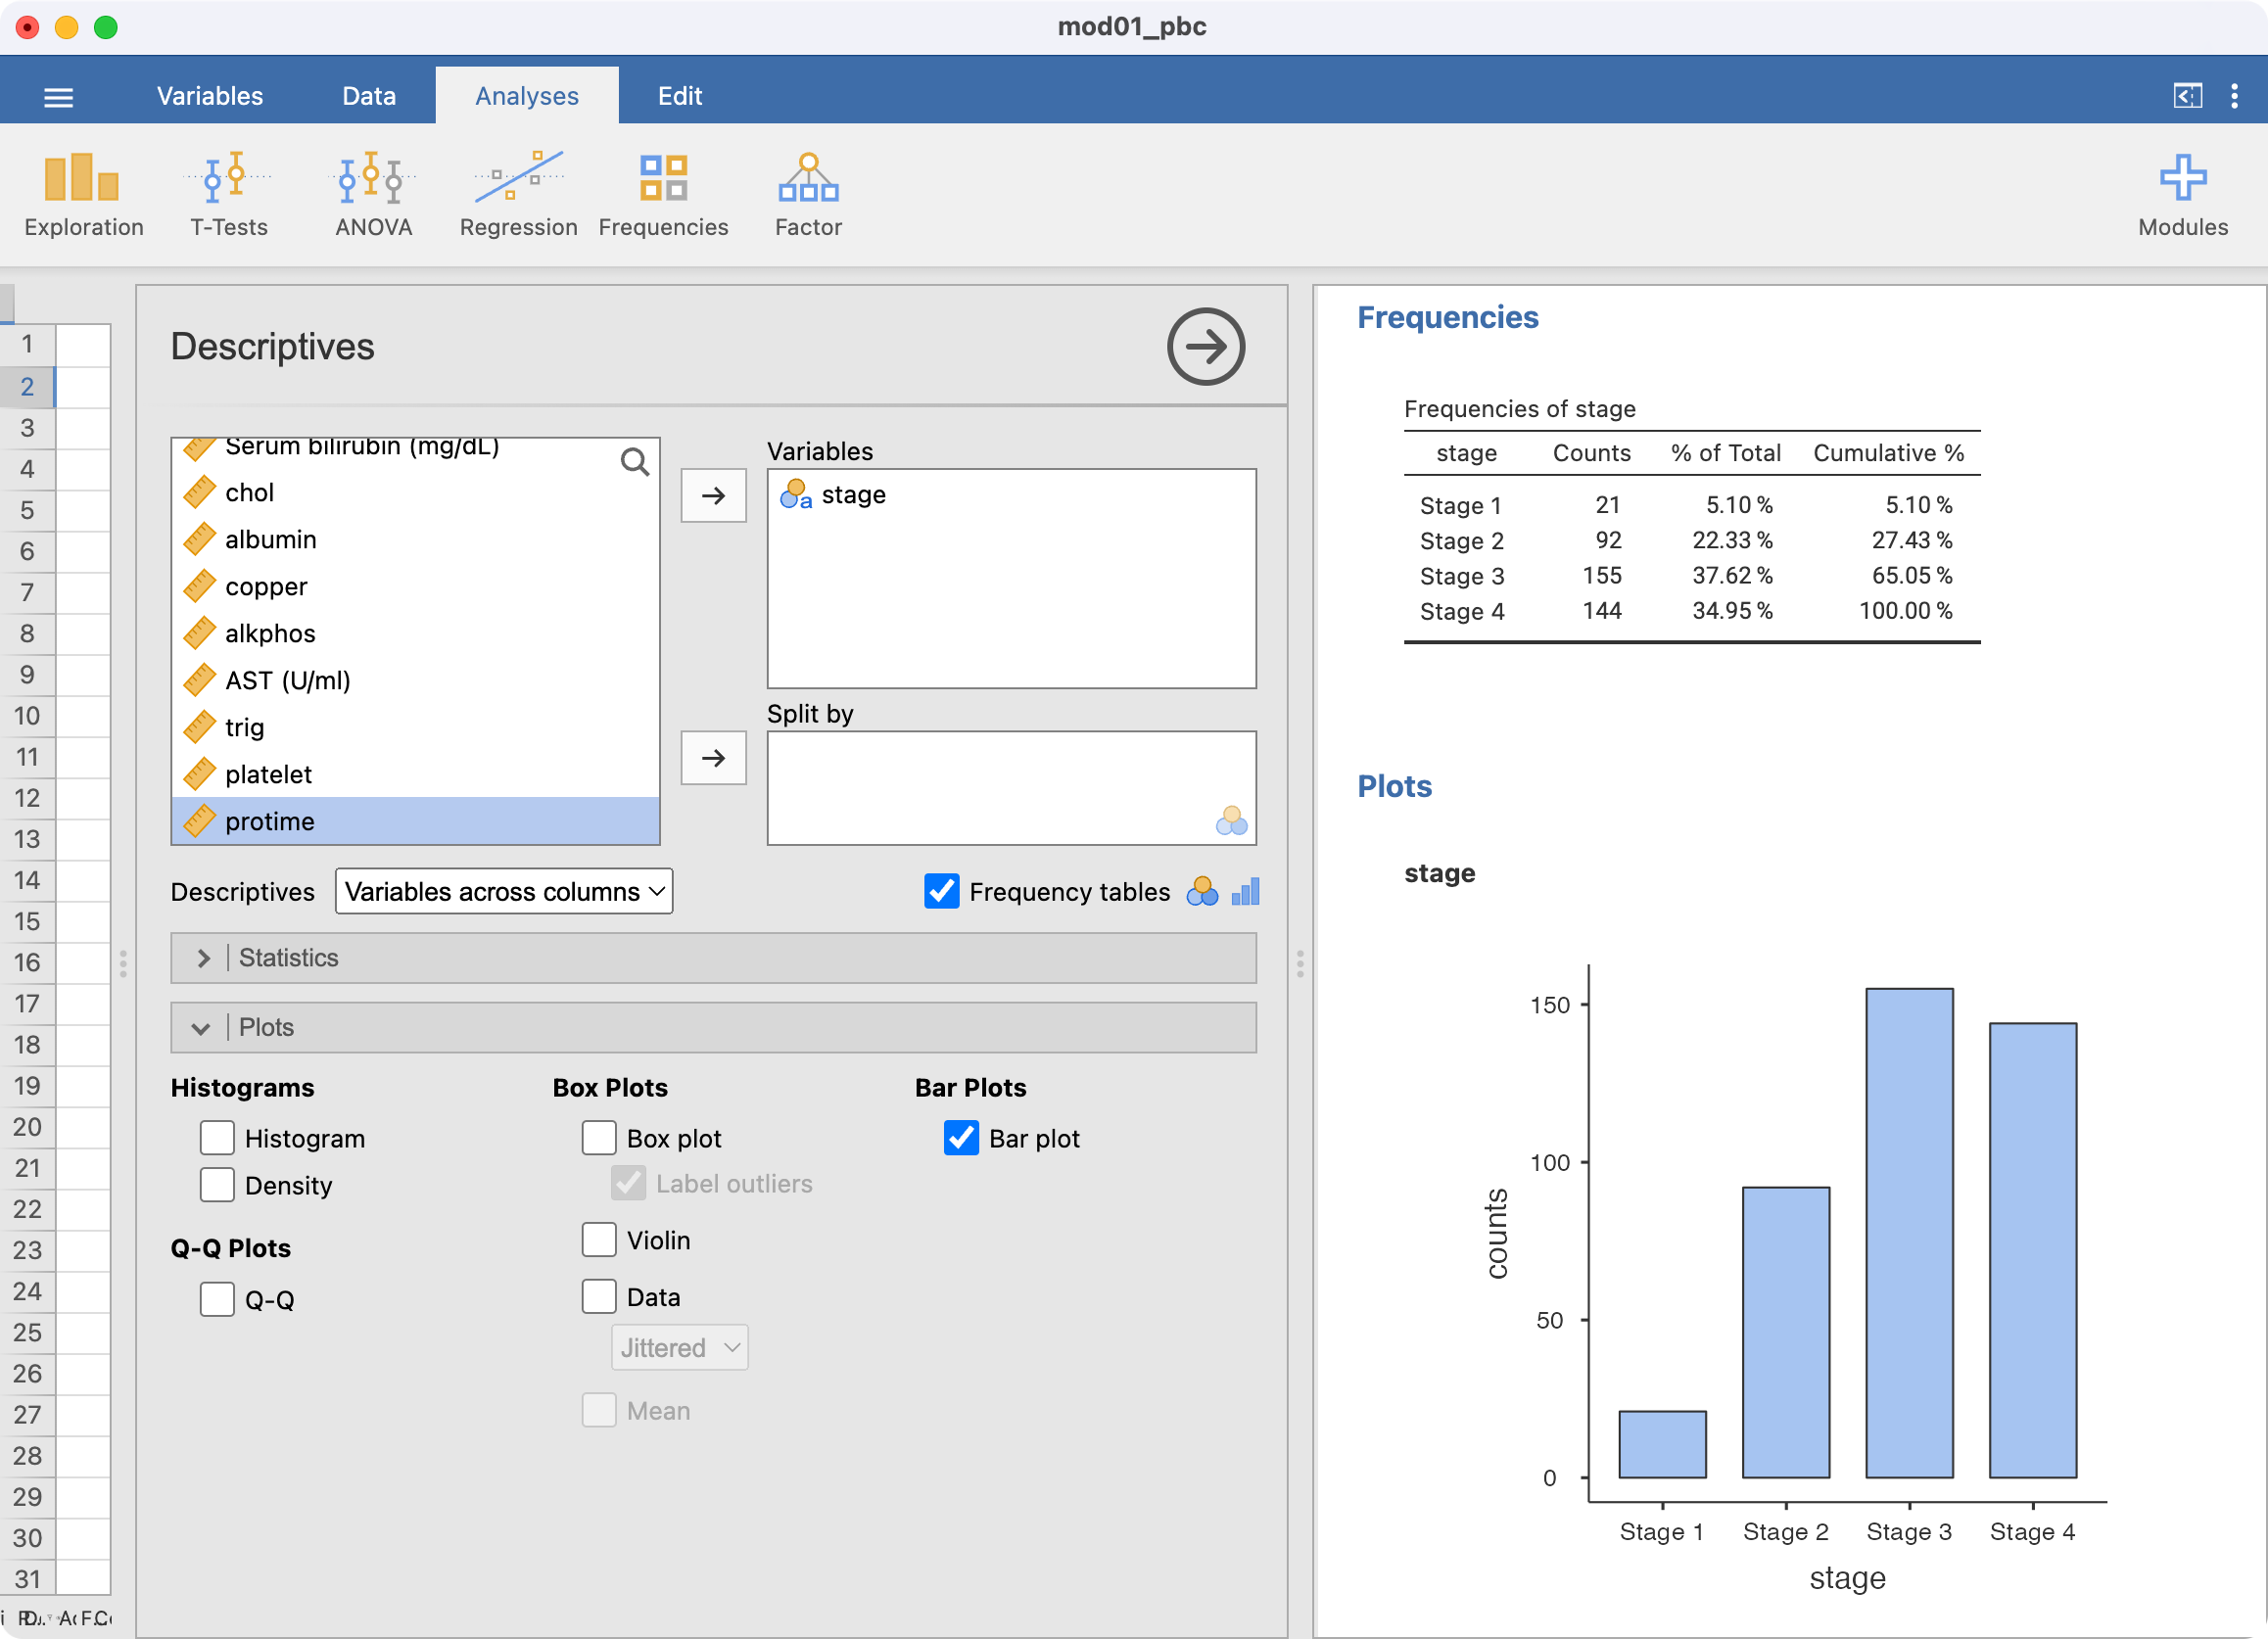
\includegraphics[keepaspectratio]{img/mod02/jamovi/mod02-barchart01.png}}

\section{Creating bar charts for two categorical
variables}\label{creating-bar-charts-for-two-categorical-variables}

\subsection{Option 1: Using Contingency Tables
command}\label{option-1-using-contingency-tables-command}

Creating a \textbf{clustered bar chart} as shown in
Figure~\ref{fig-bar-2} can be done using \textbf{Analyses \textgreater{}
Frequencies \textgreater{} Contingency Tables \textgreater{} Independent
Samples}. First create the cross-tab of interest, for example, Stage by
Sex. Choose \textbf{Plots \textgreater{} Bar Plot}, and ensure the Bar
Type is selected as \textbf{Side by side}. Choose the X-axis as required
- here we want to see stage on the x-axis, so we choose the x-axis to be
columns (this may need to be adjusted according to how your table has
been set up):

\pandocbounded{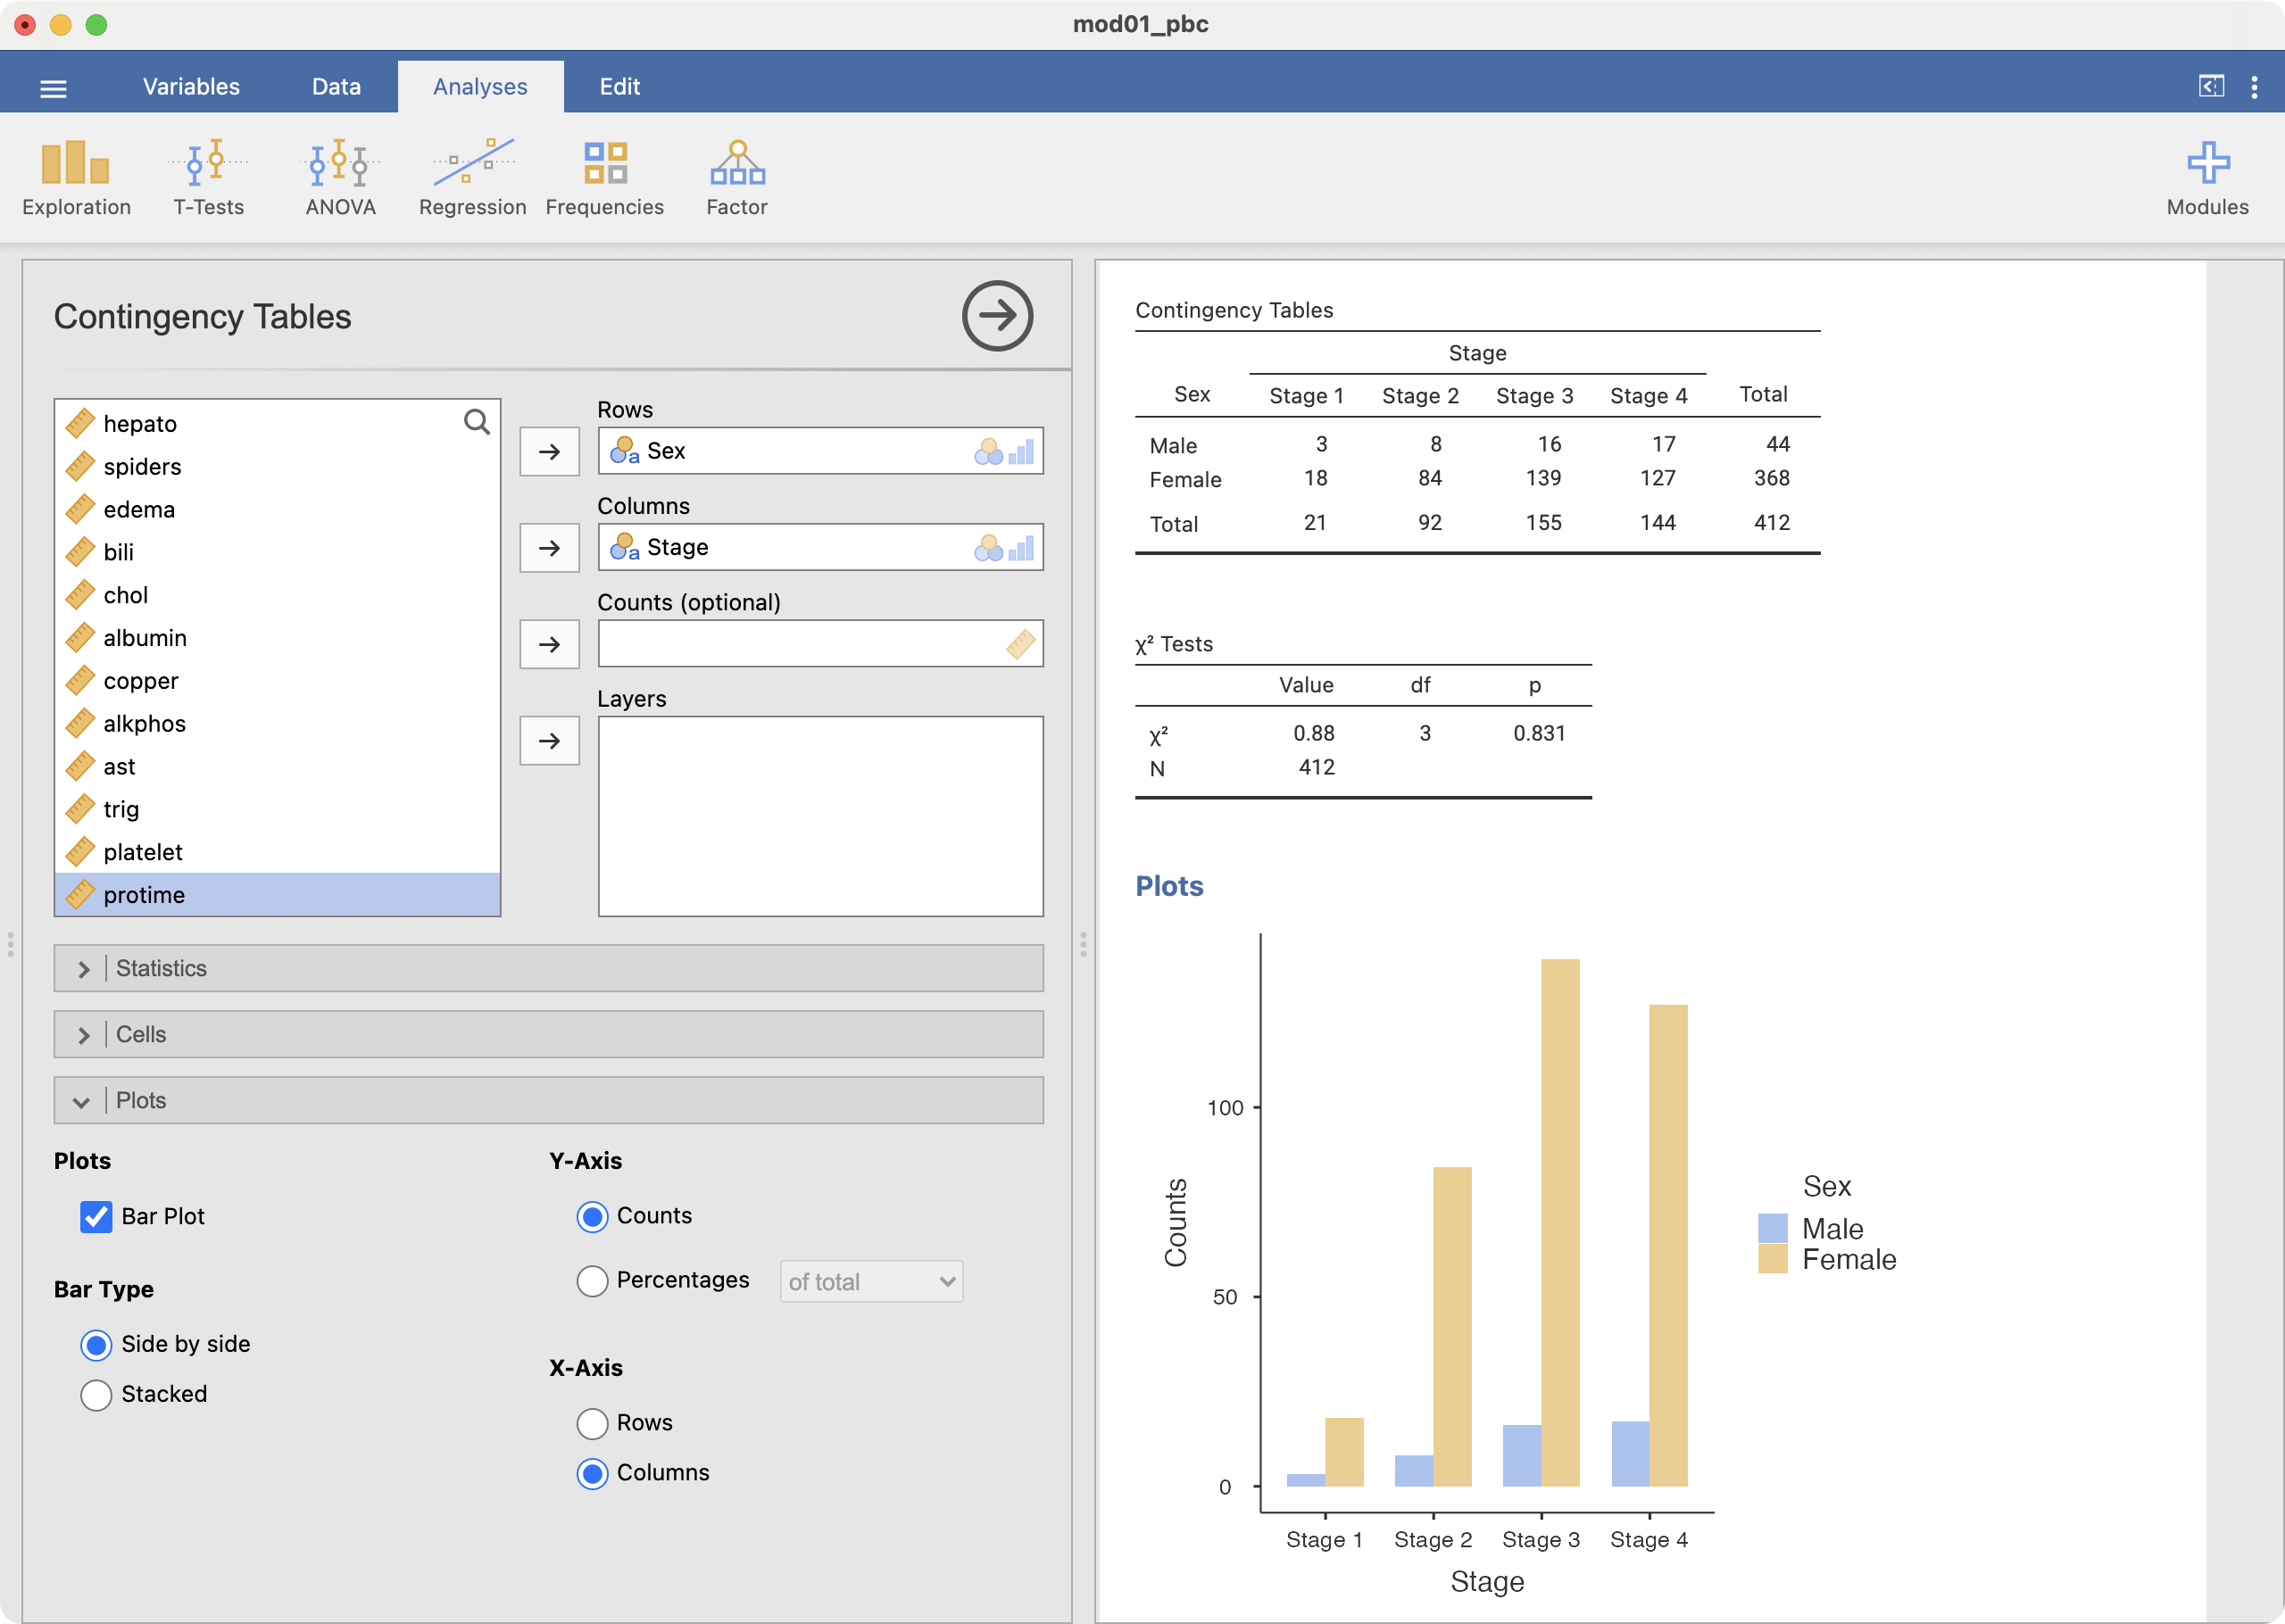
\includegraphics[keepaspectratio]{img/mod02/jamovi/mod02-clustered.png}}
To create a \textbf{stacked bar chart} (as in Figure~\ref{fig-bar-3}),
choose the Bar Type to be \textbf{Stacked}:

\pandocbounded{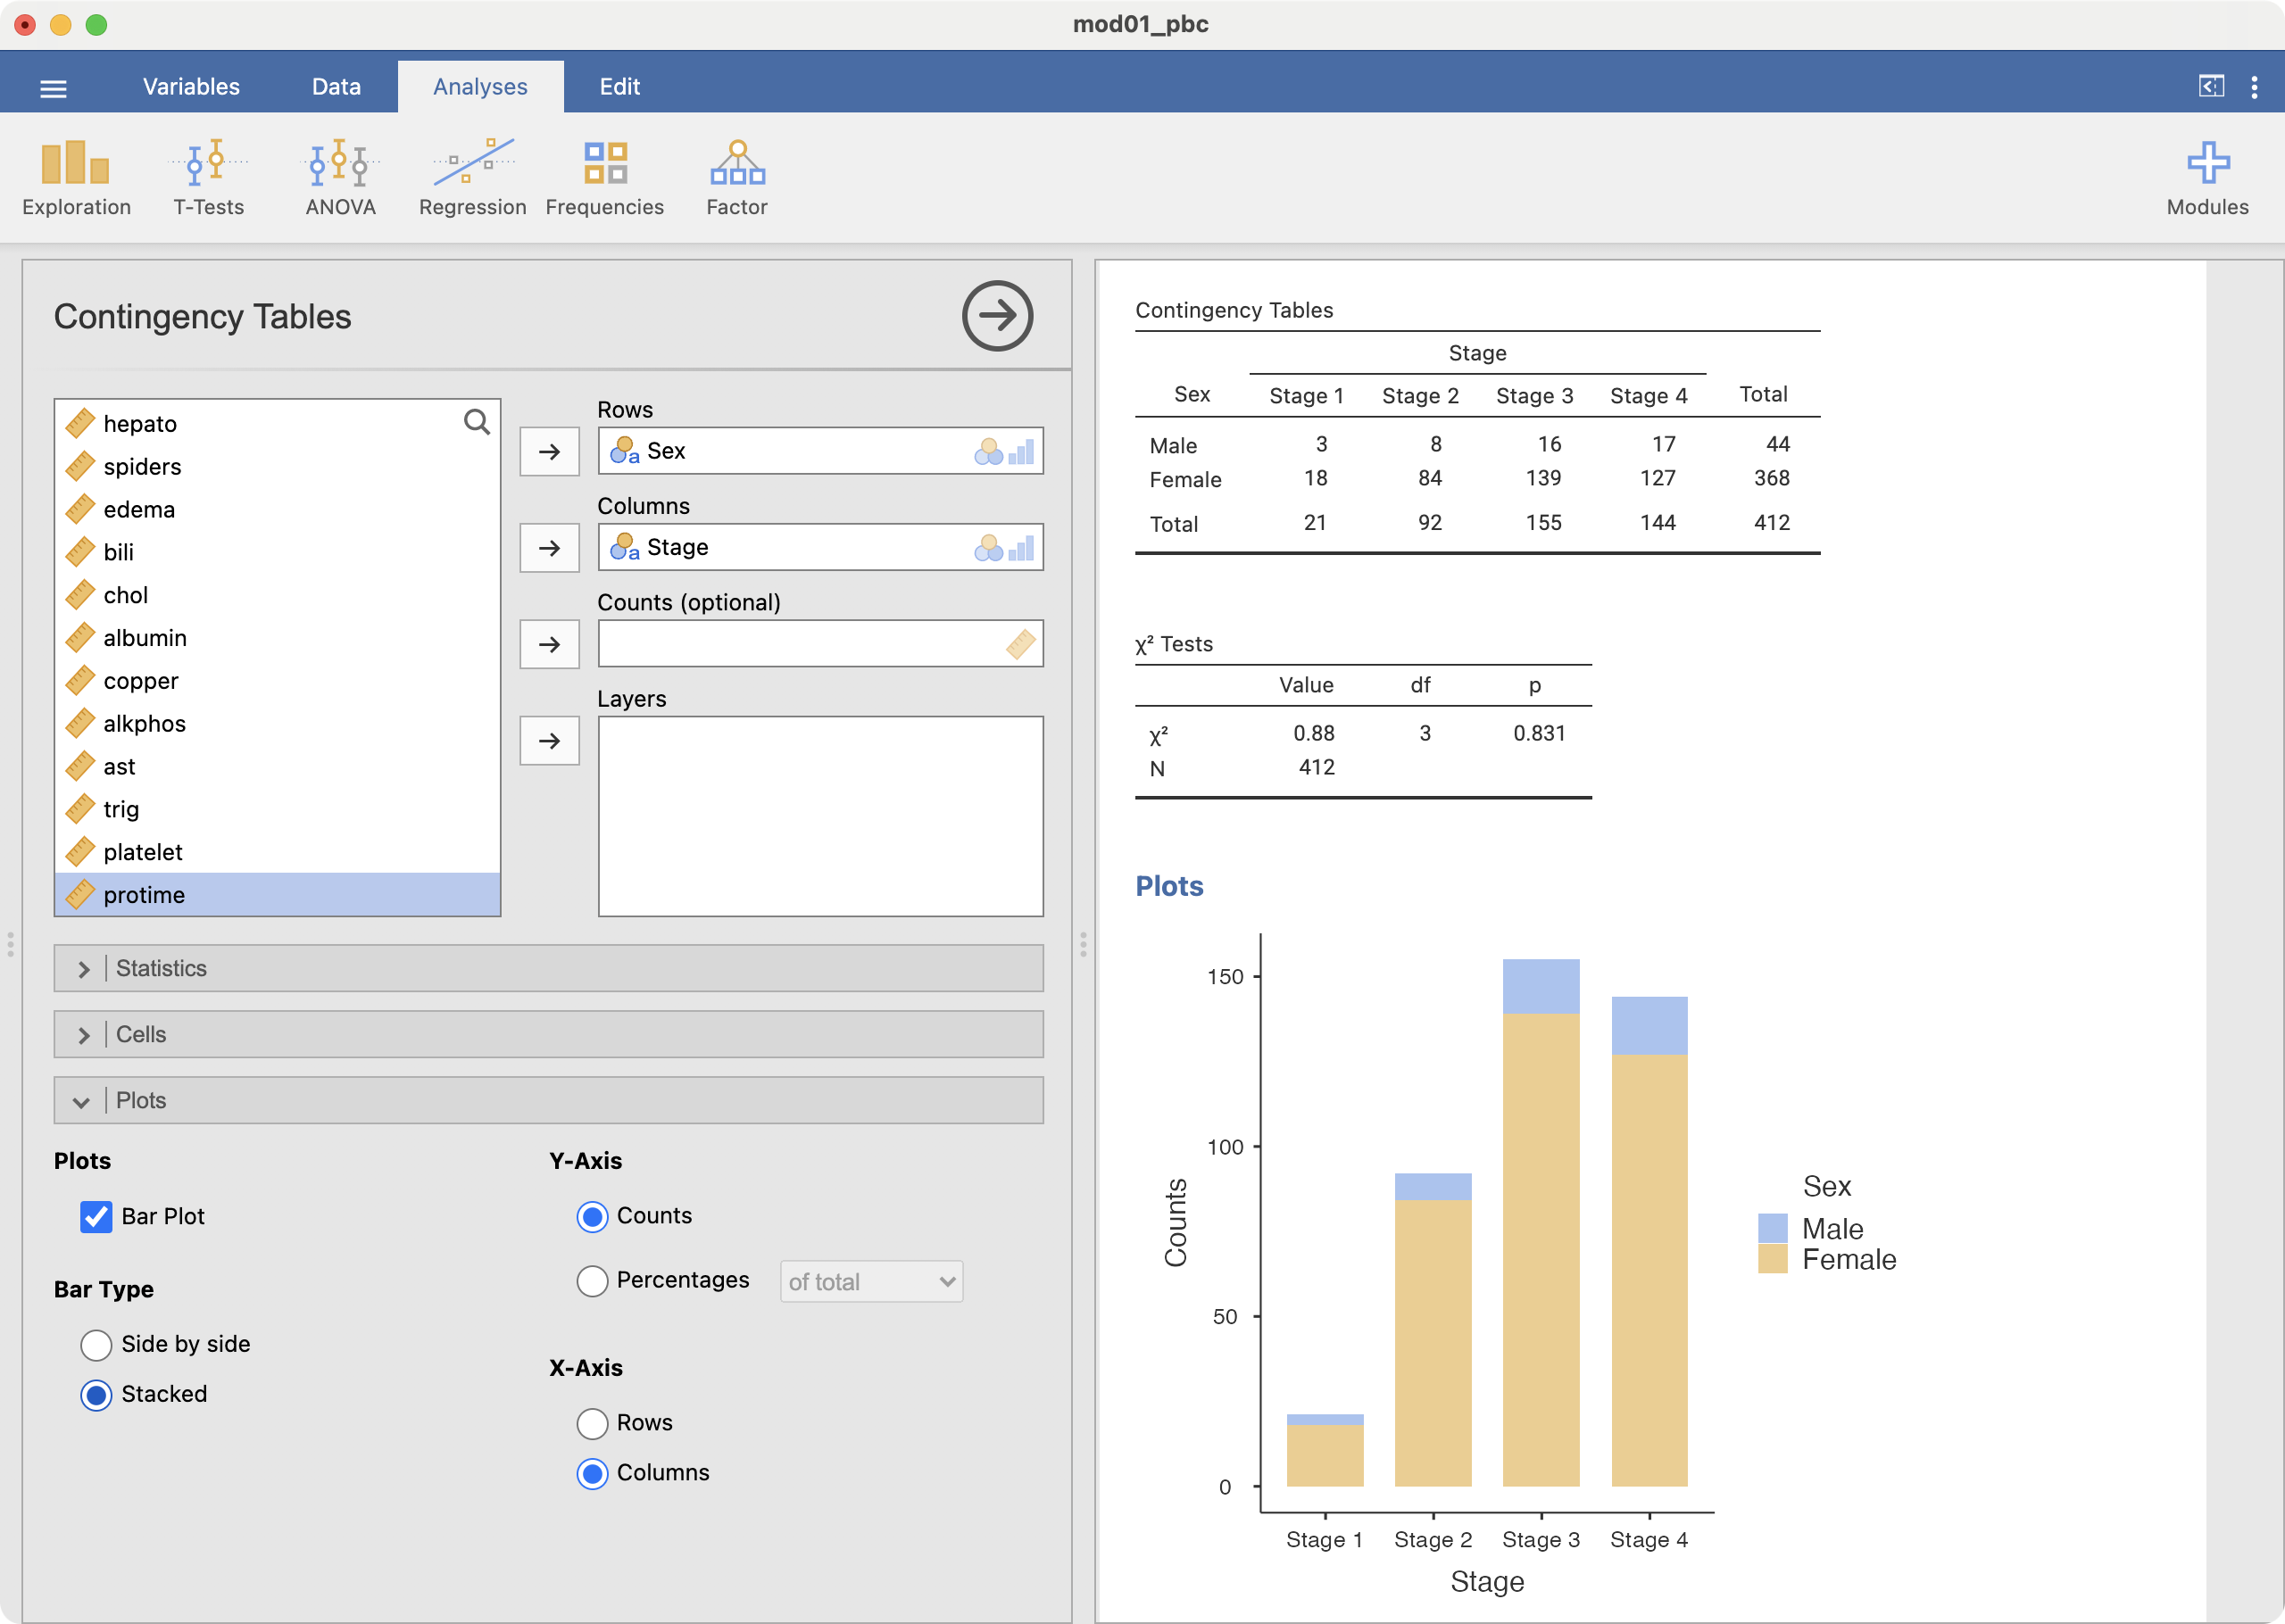
\includegraphics[keepaspectratio]{img/mod02/jamovi/mod02-stacked.png}}

Finally, to create a \textbf{stacked relative bar chart} (as in
Figure~\ref{fig-bar-4}), choose the Y-axis to be \textbf{Percentages
within column}:

\pandocbounded{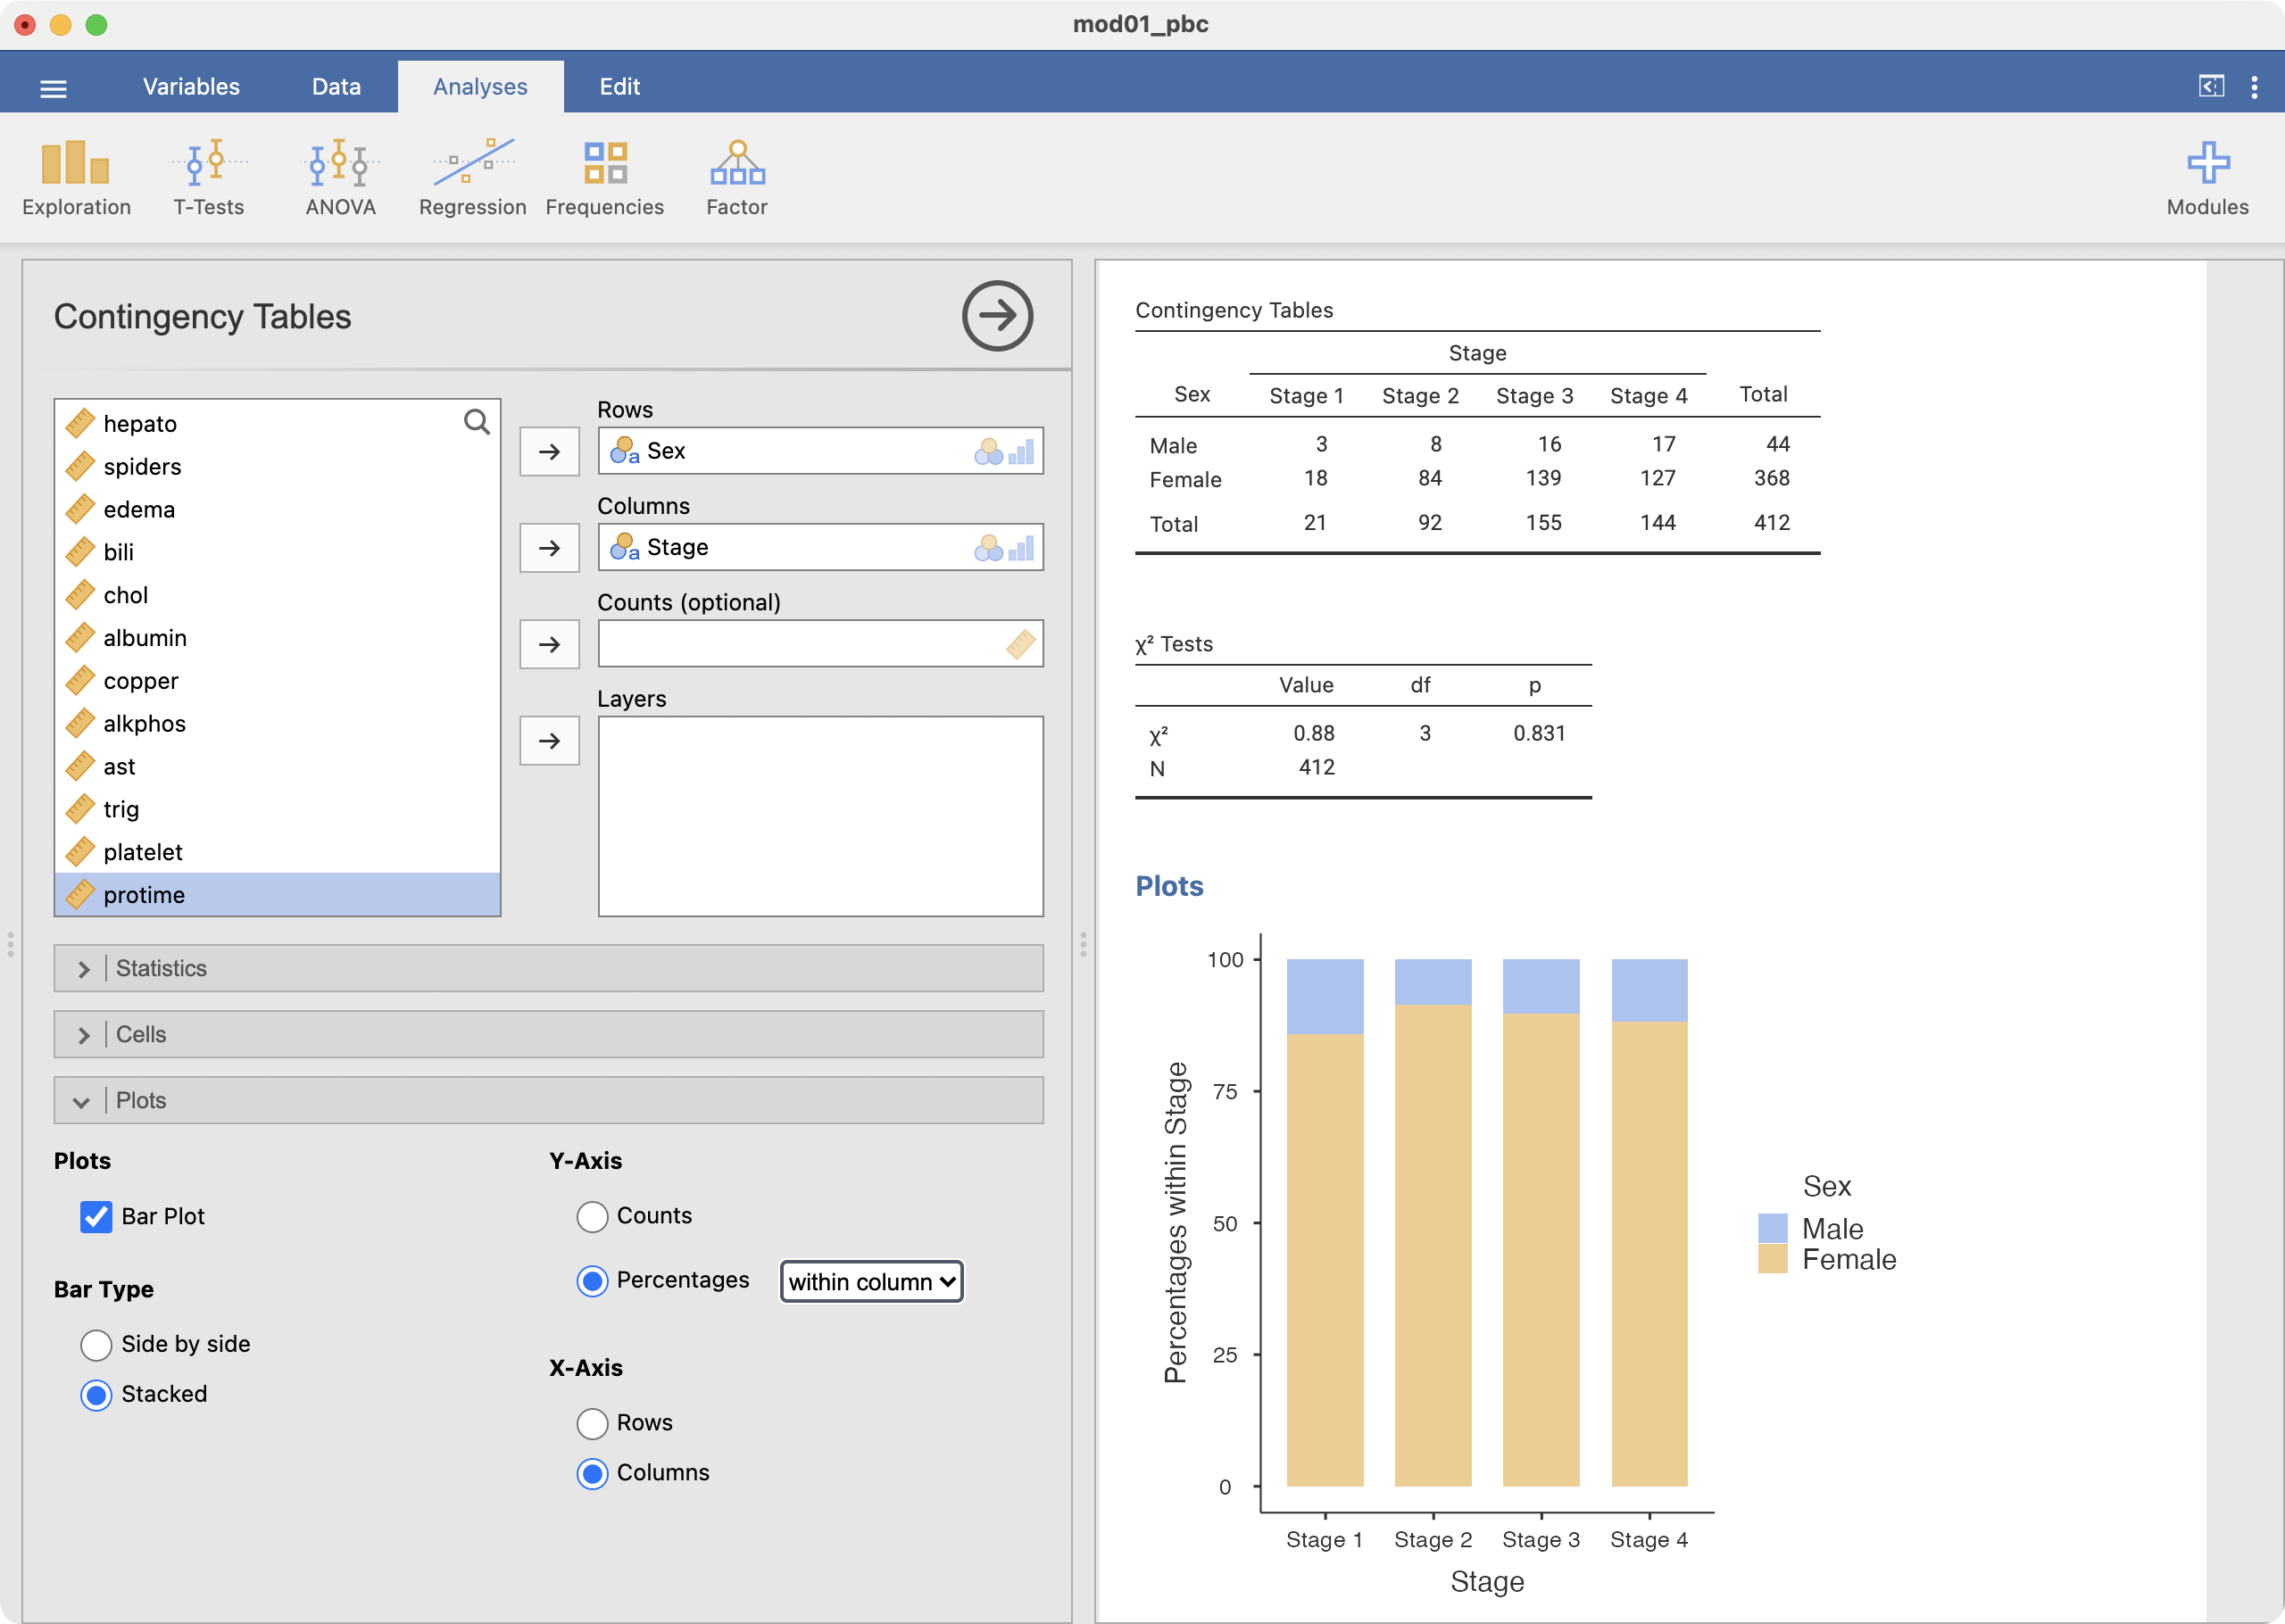
\includegraphics[keepaspectratio]{img/mod02/jamovi/mod02-stacked-rel.png}}

\subsection{Option 2: Using Survey Plots
command}\label{option-2-using-survey-plots-command}

An alternative way of producing barcharts is via a Module called
\textbf{surveymv} that we add to jamovi. To install the module, click
the \textbf{Analyses} tab, and click the large \textbf{+} at the
top-right of the window. Choose \textbf{jamovi library}:

\pandocbounded{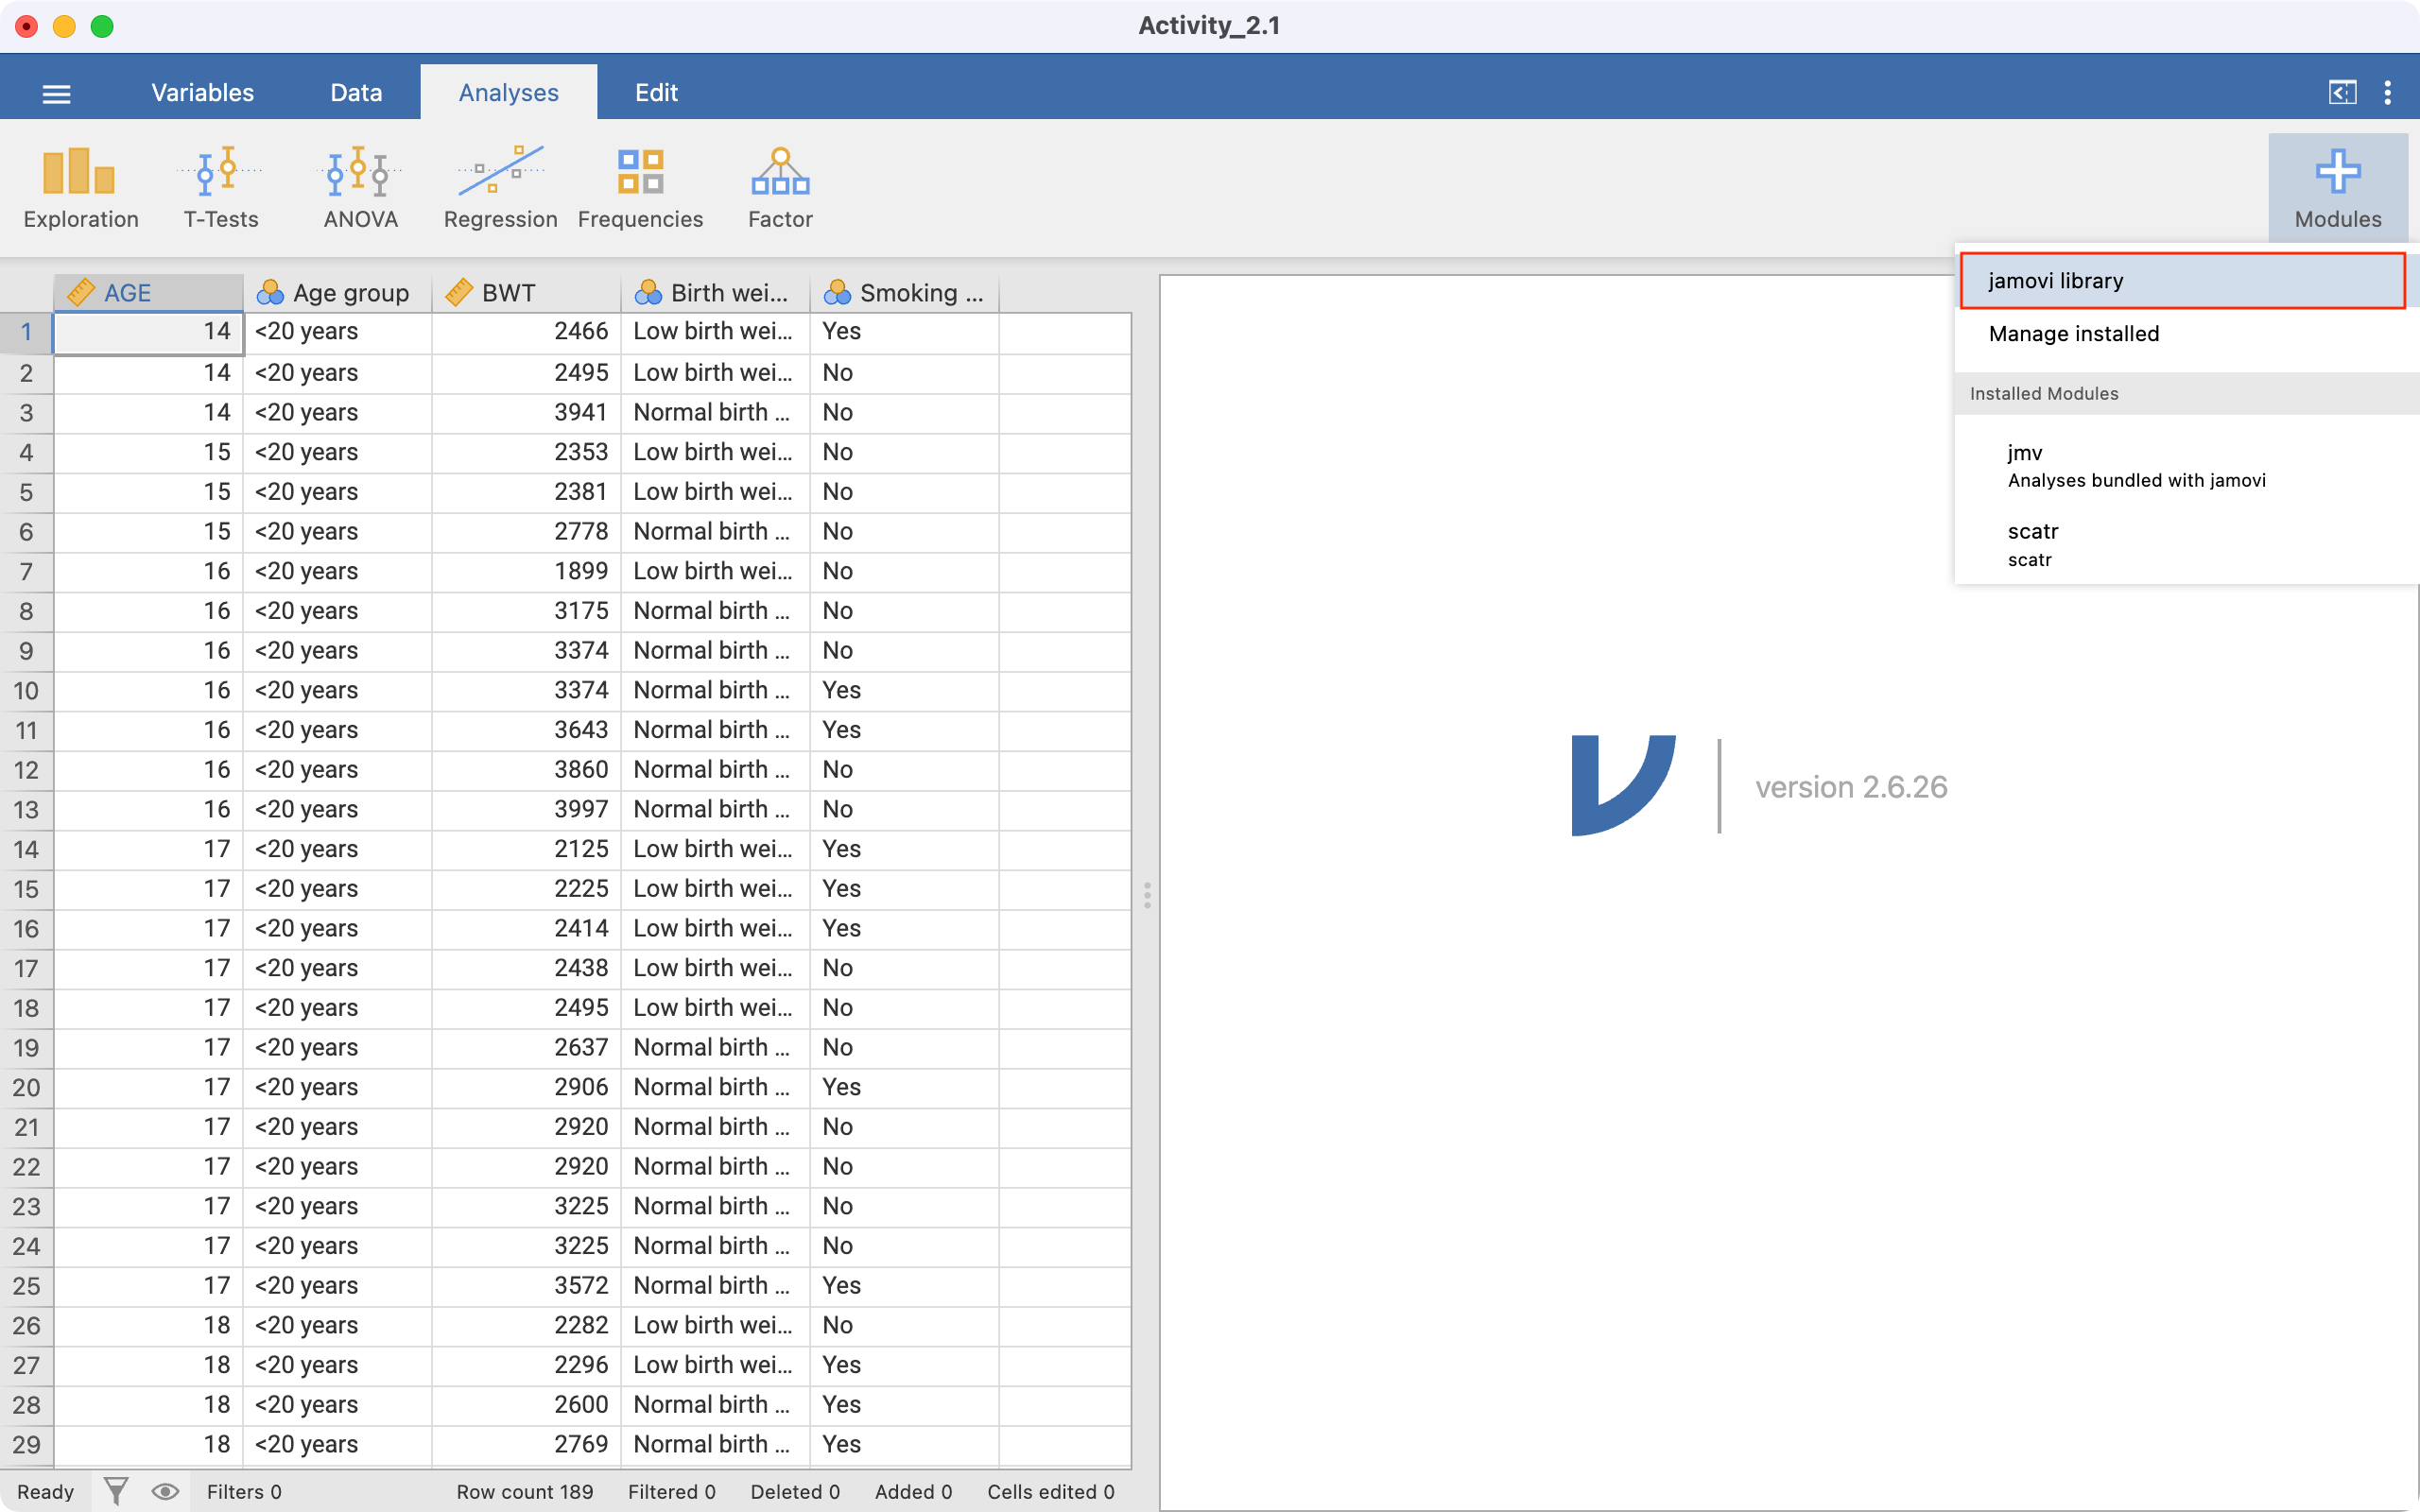
\includegraphics[keepaspectratio]{img/mod02/jamovi/act2.1.2.png}}

Click \textbf{Available} and search for \texttt{surveymv}, then click
install:

\pandocbounded{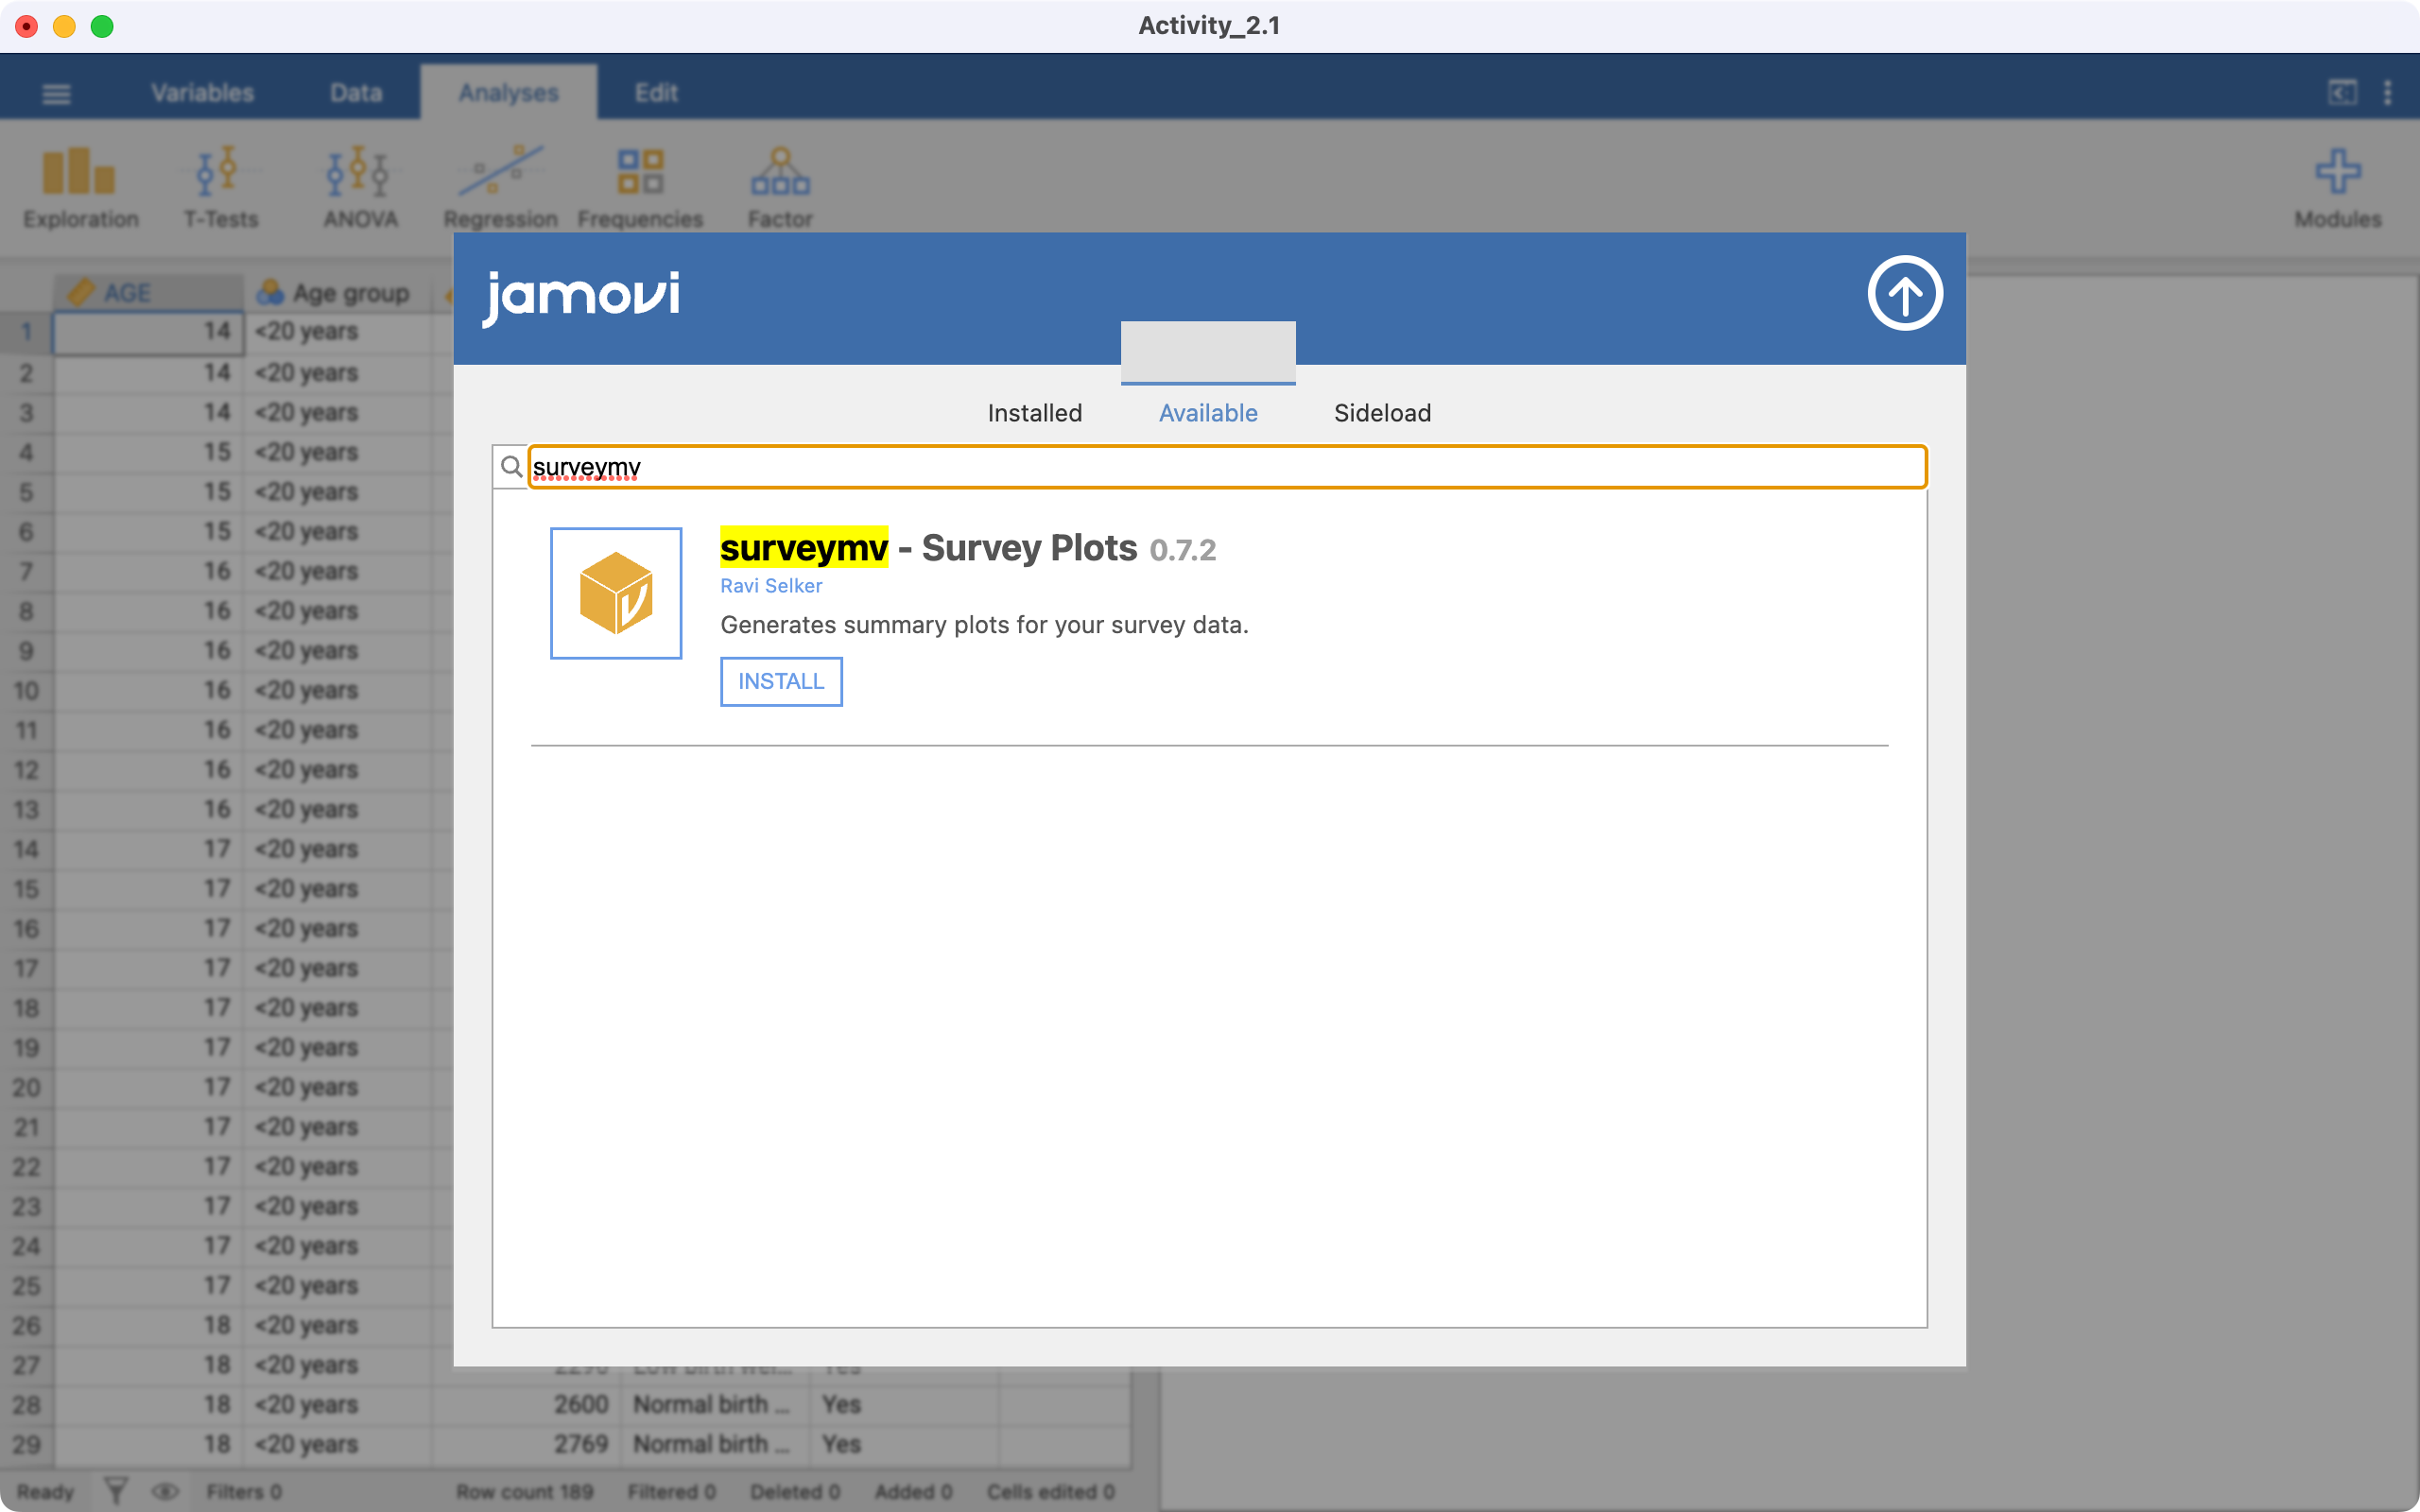
\includegraphics[keepaspectratio]{img/mod02/jamovi/act2.1.3.png}}

The module has now been installed. To run the module, click the up-arrow
to return to the \textbf{Analyses} tab, click the large \textbf{+} and
choose \textbf{surveymv \textgreater{} Survey Plots}:

\pandocbounded{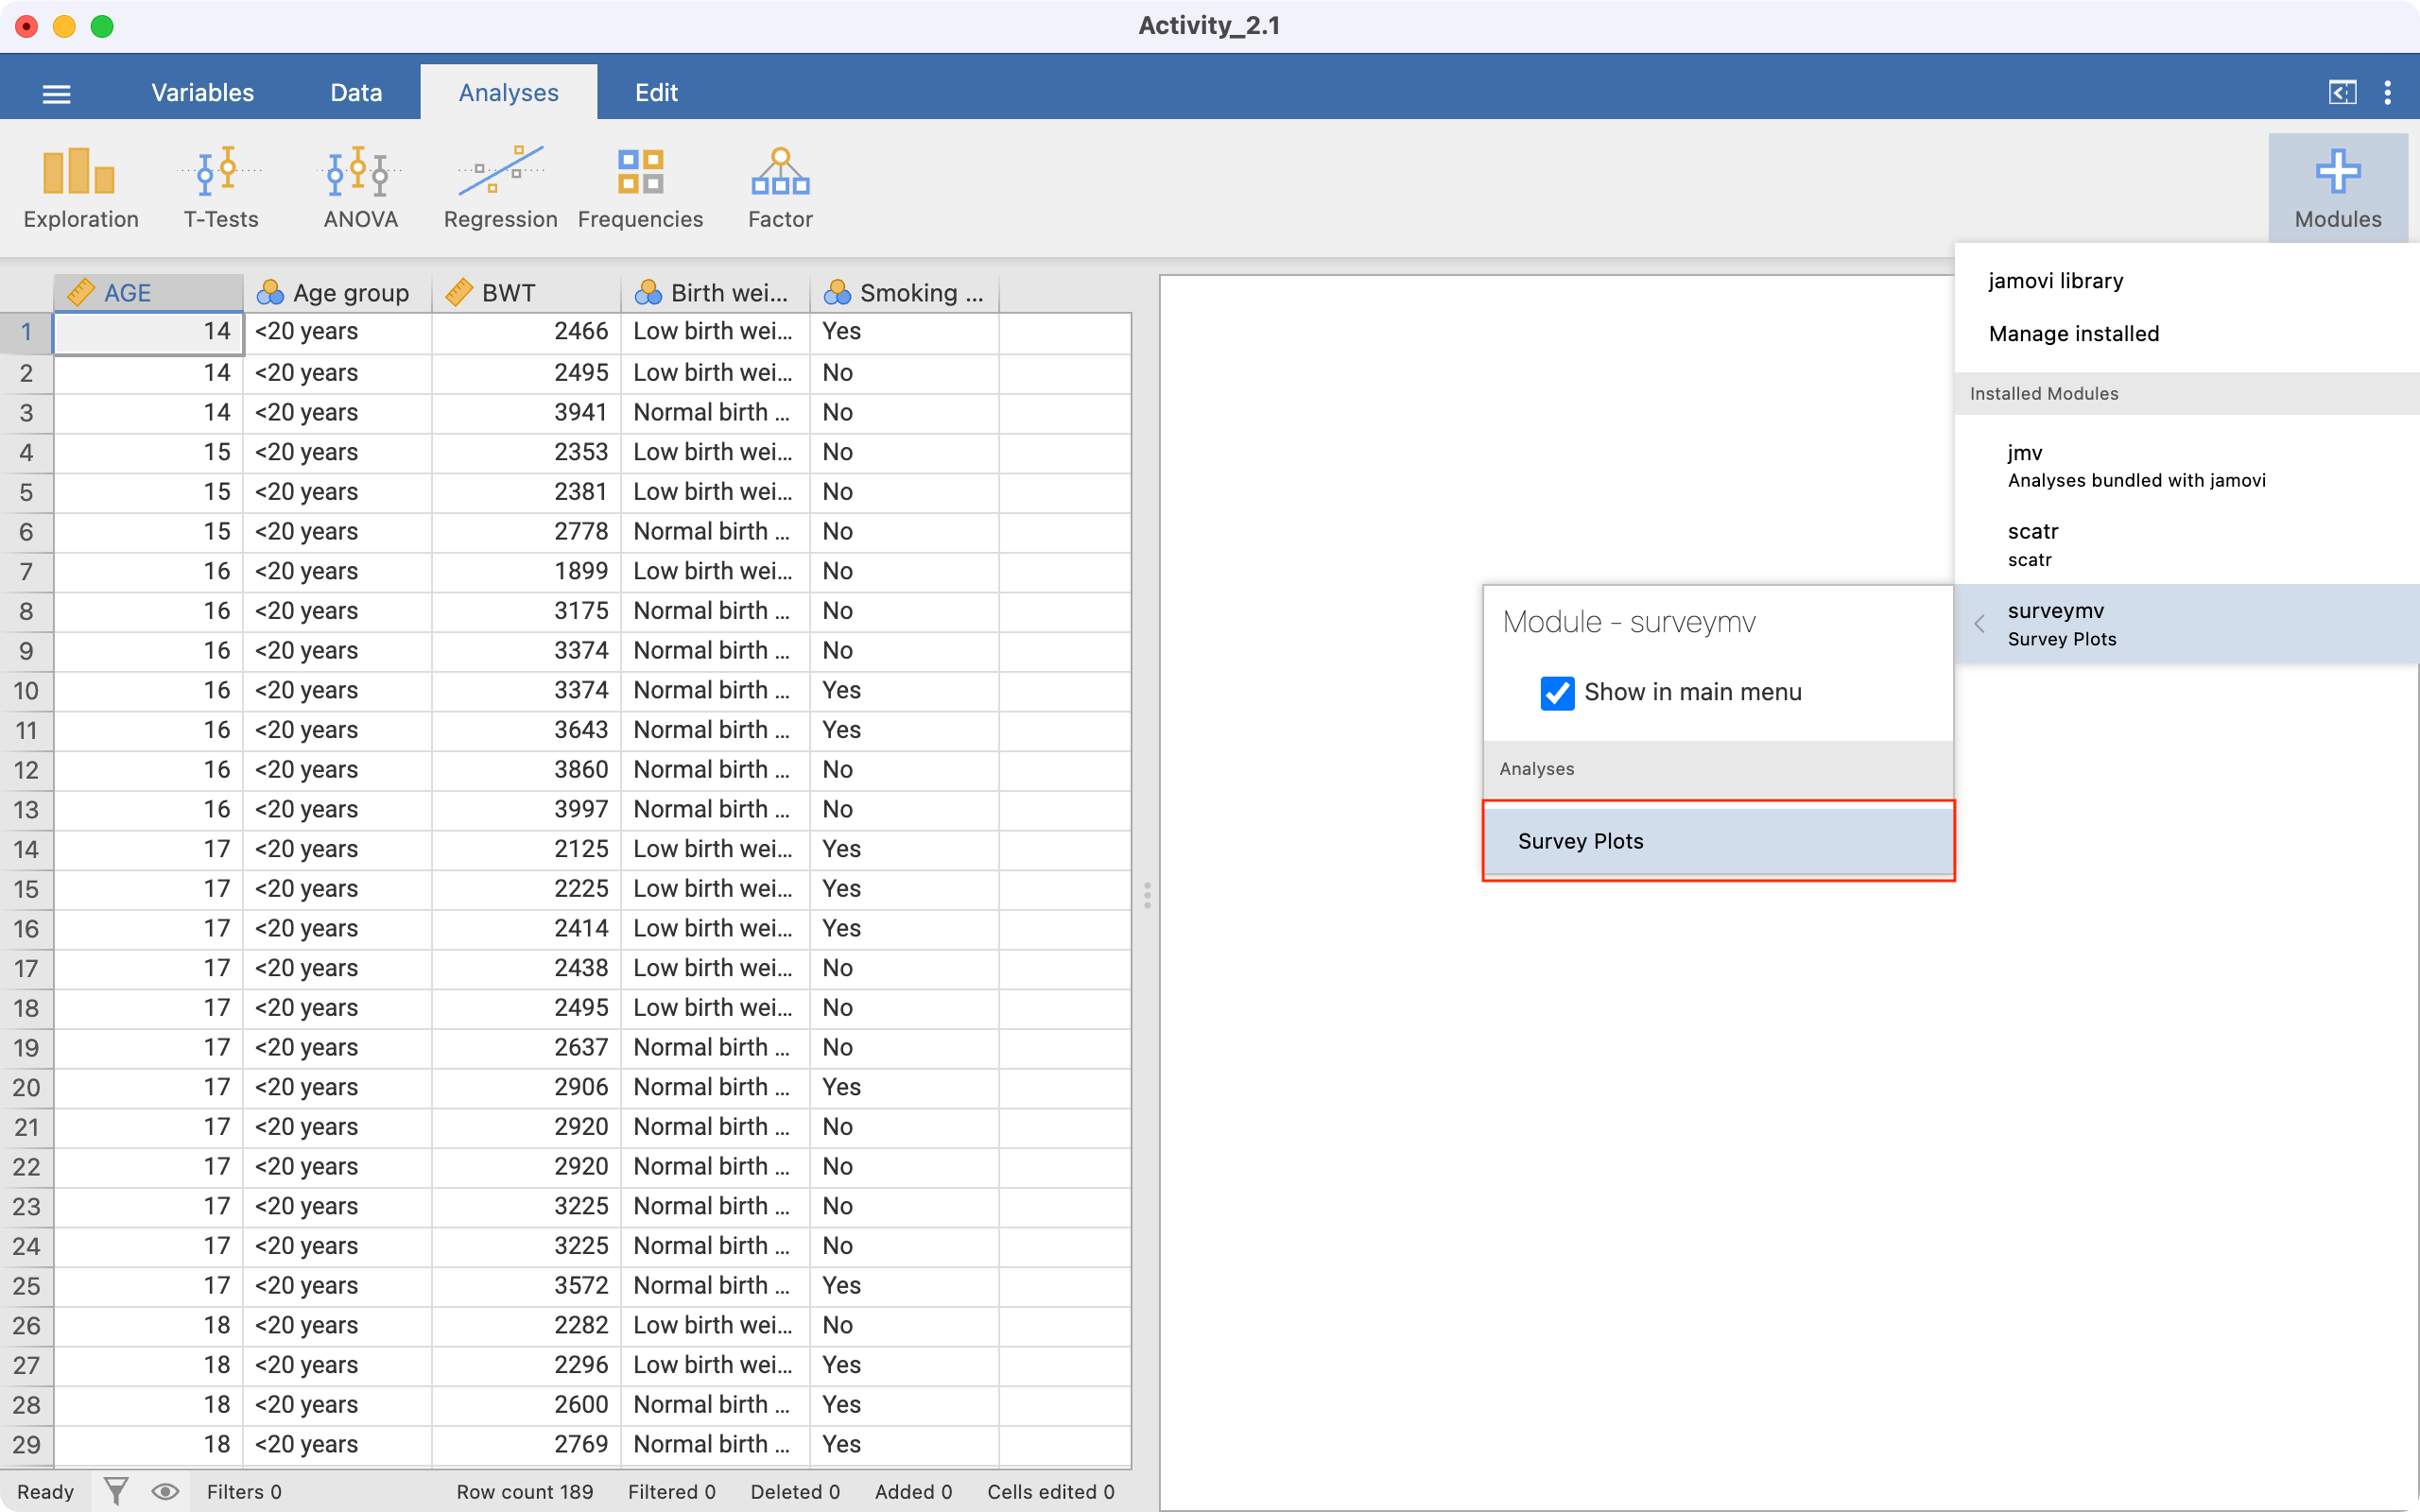
\includegraphics[keepaspectratio]{img/mod02/jamovi/act2.1.4.png}}

We will demonstrate the module by recreating Figure~\ref{fig-bar-4}, a
figure of the relative frequencies of sex within stage of disease. To
open the module options, click the large \textbf{+} and choose
\textbf{surveymv \textgreater{} Survey Plots}:

\pandocbounded{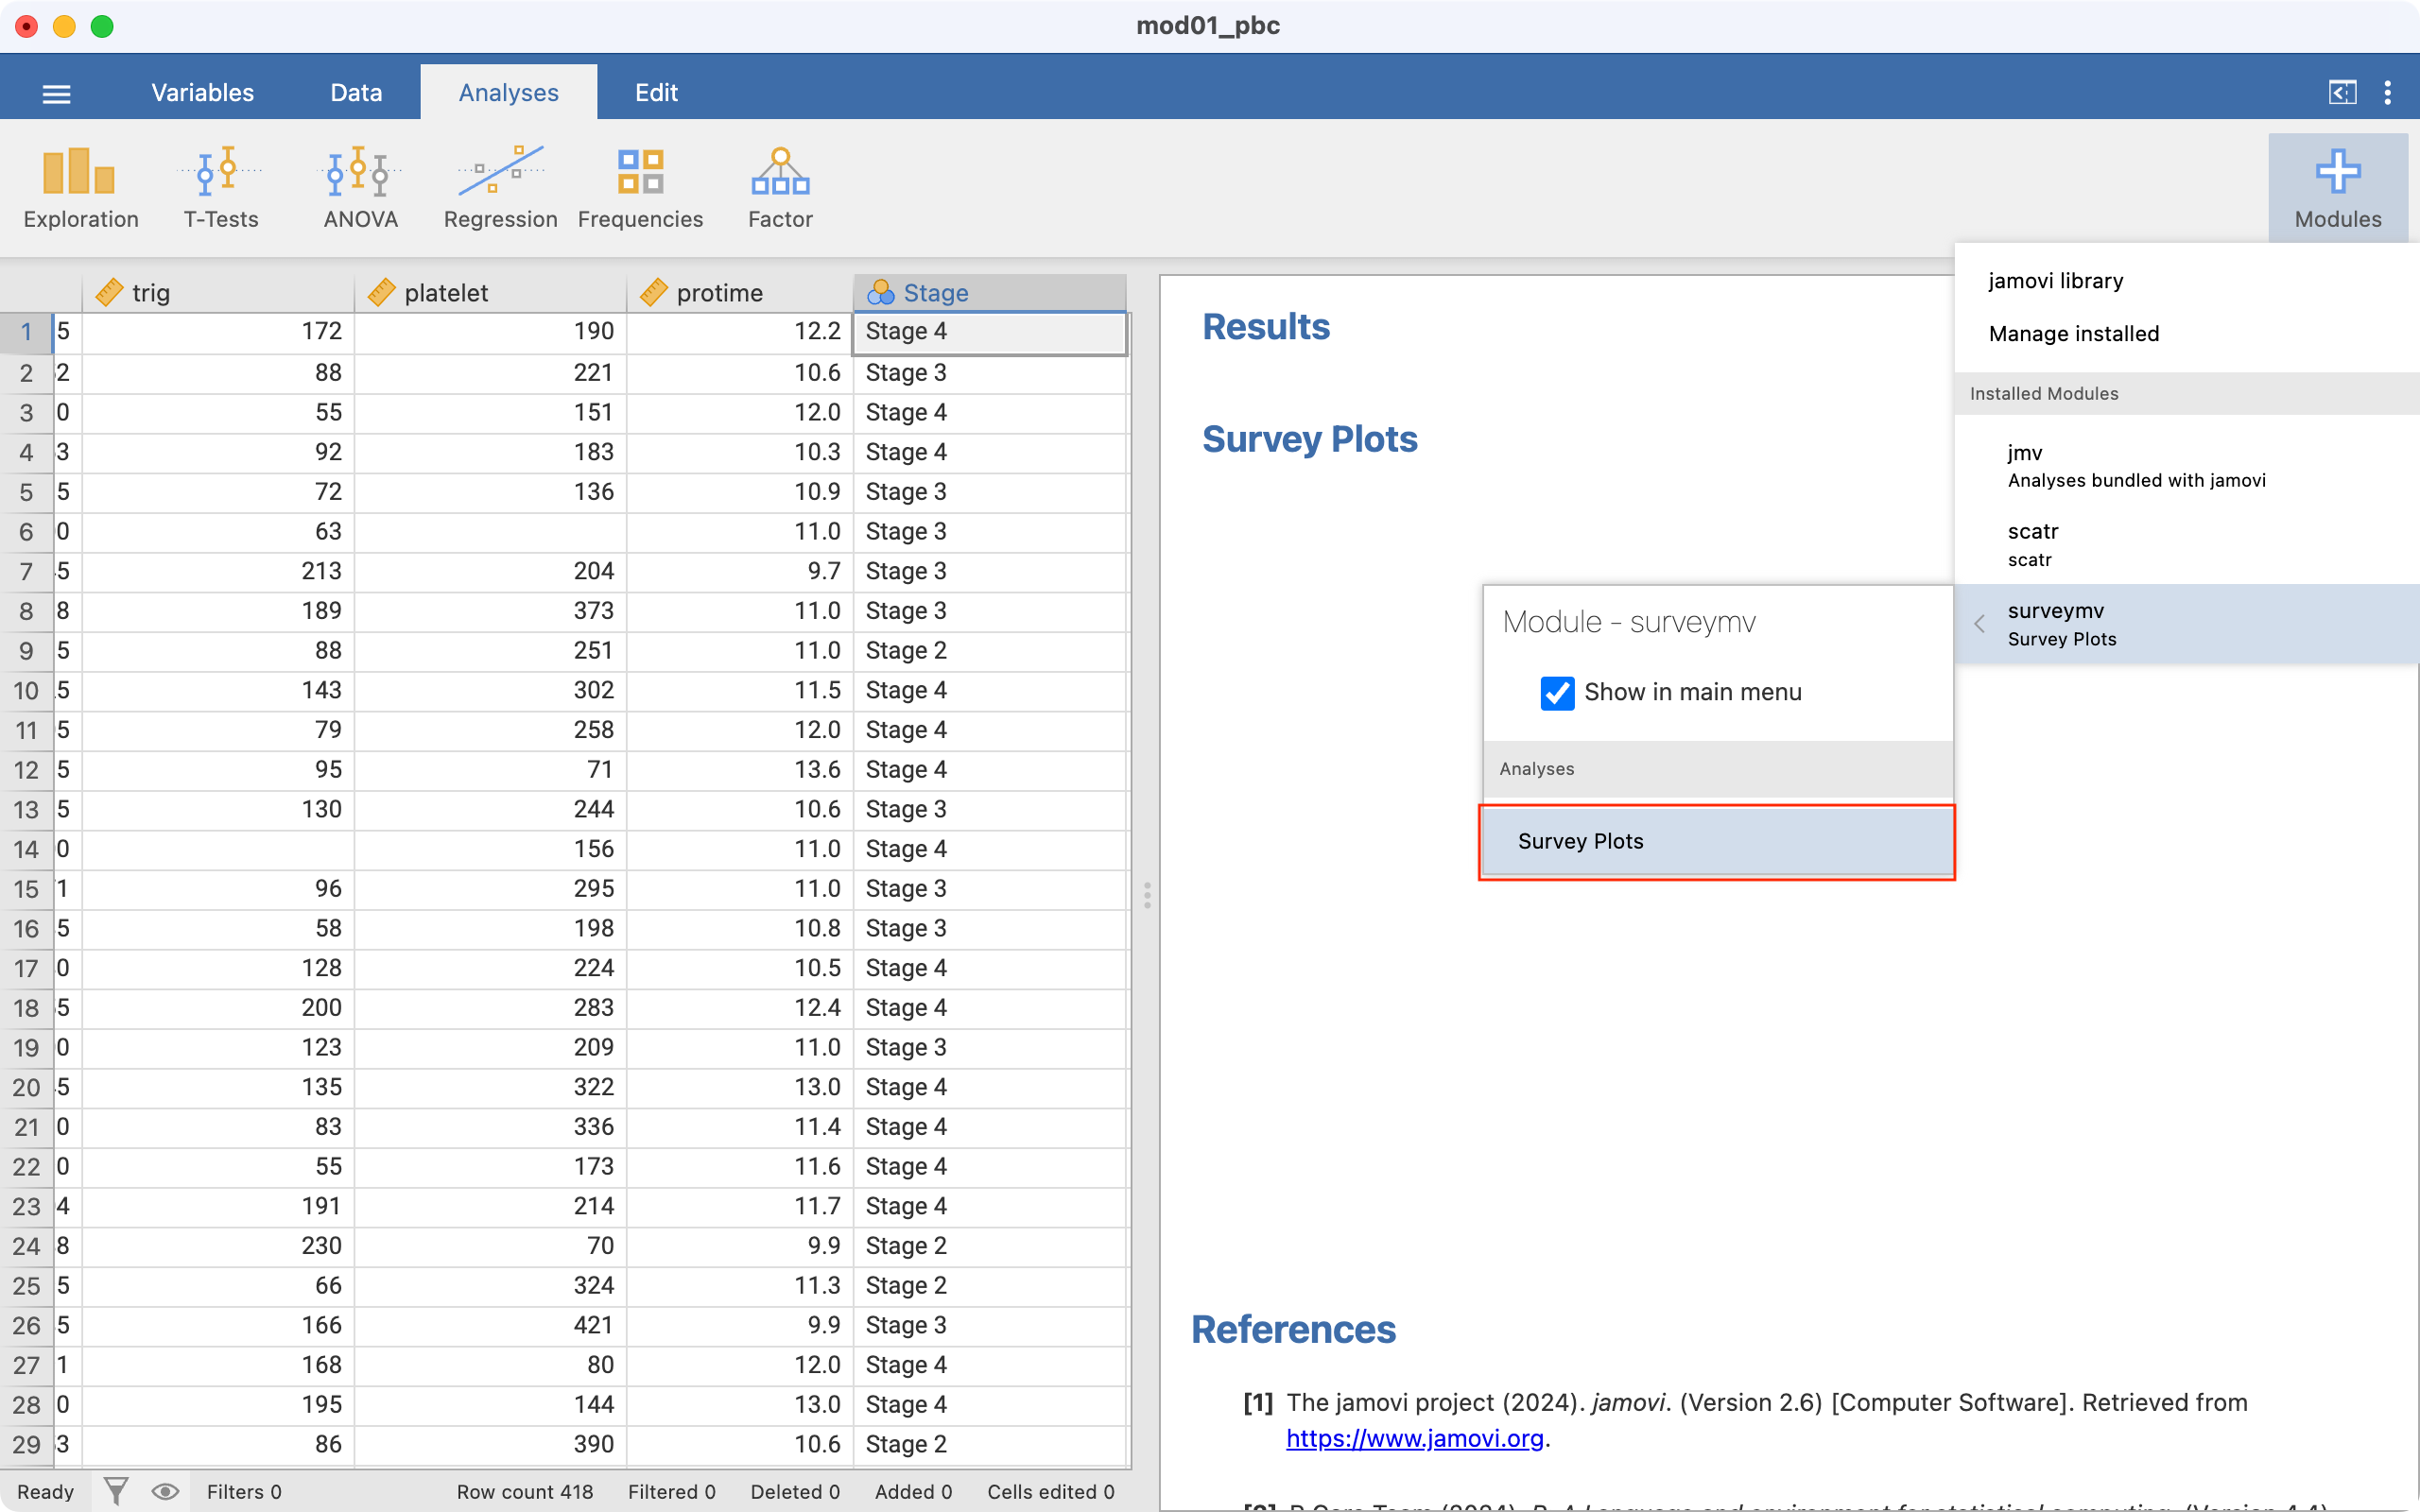
\includegraphics[keepaspectratio]{img/mod02/jamovi/surveymv-1.png}}

We choose the variable we want to plot, here \texttt{Sex}. We want to
plot sex within each stage, so \texttt{Stage} is entered as a
\textbf{Grouping Variable}:

\pandocbounded{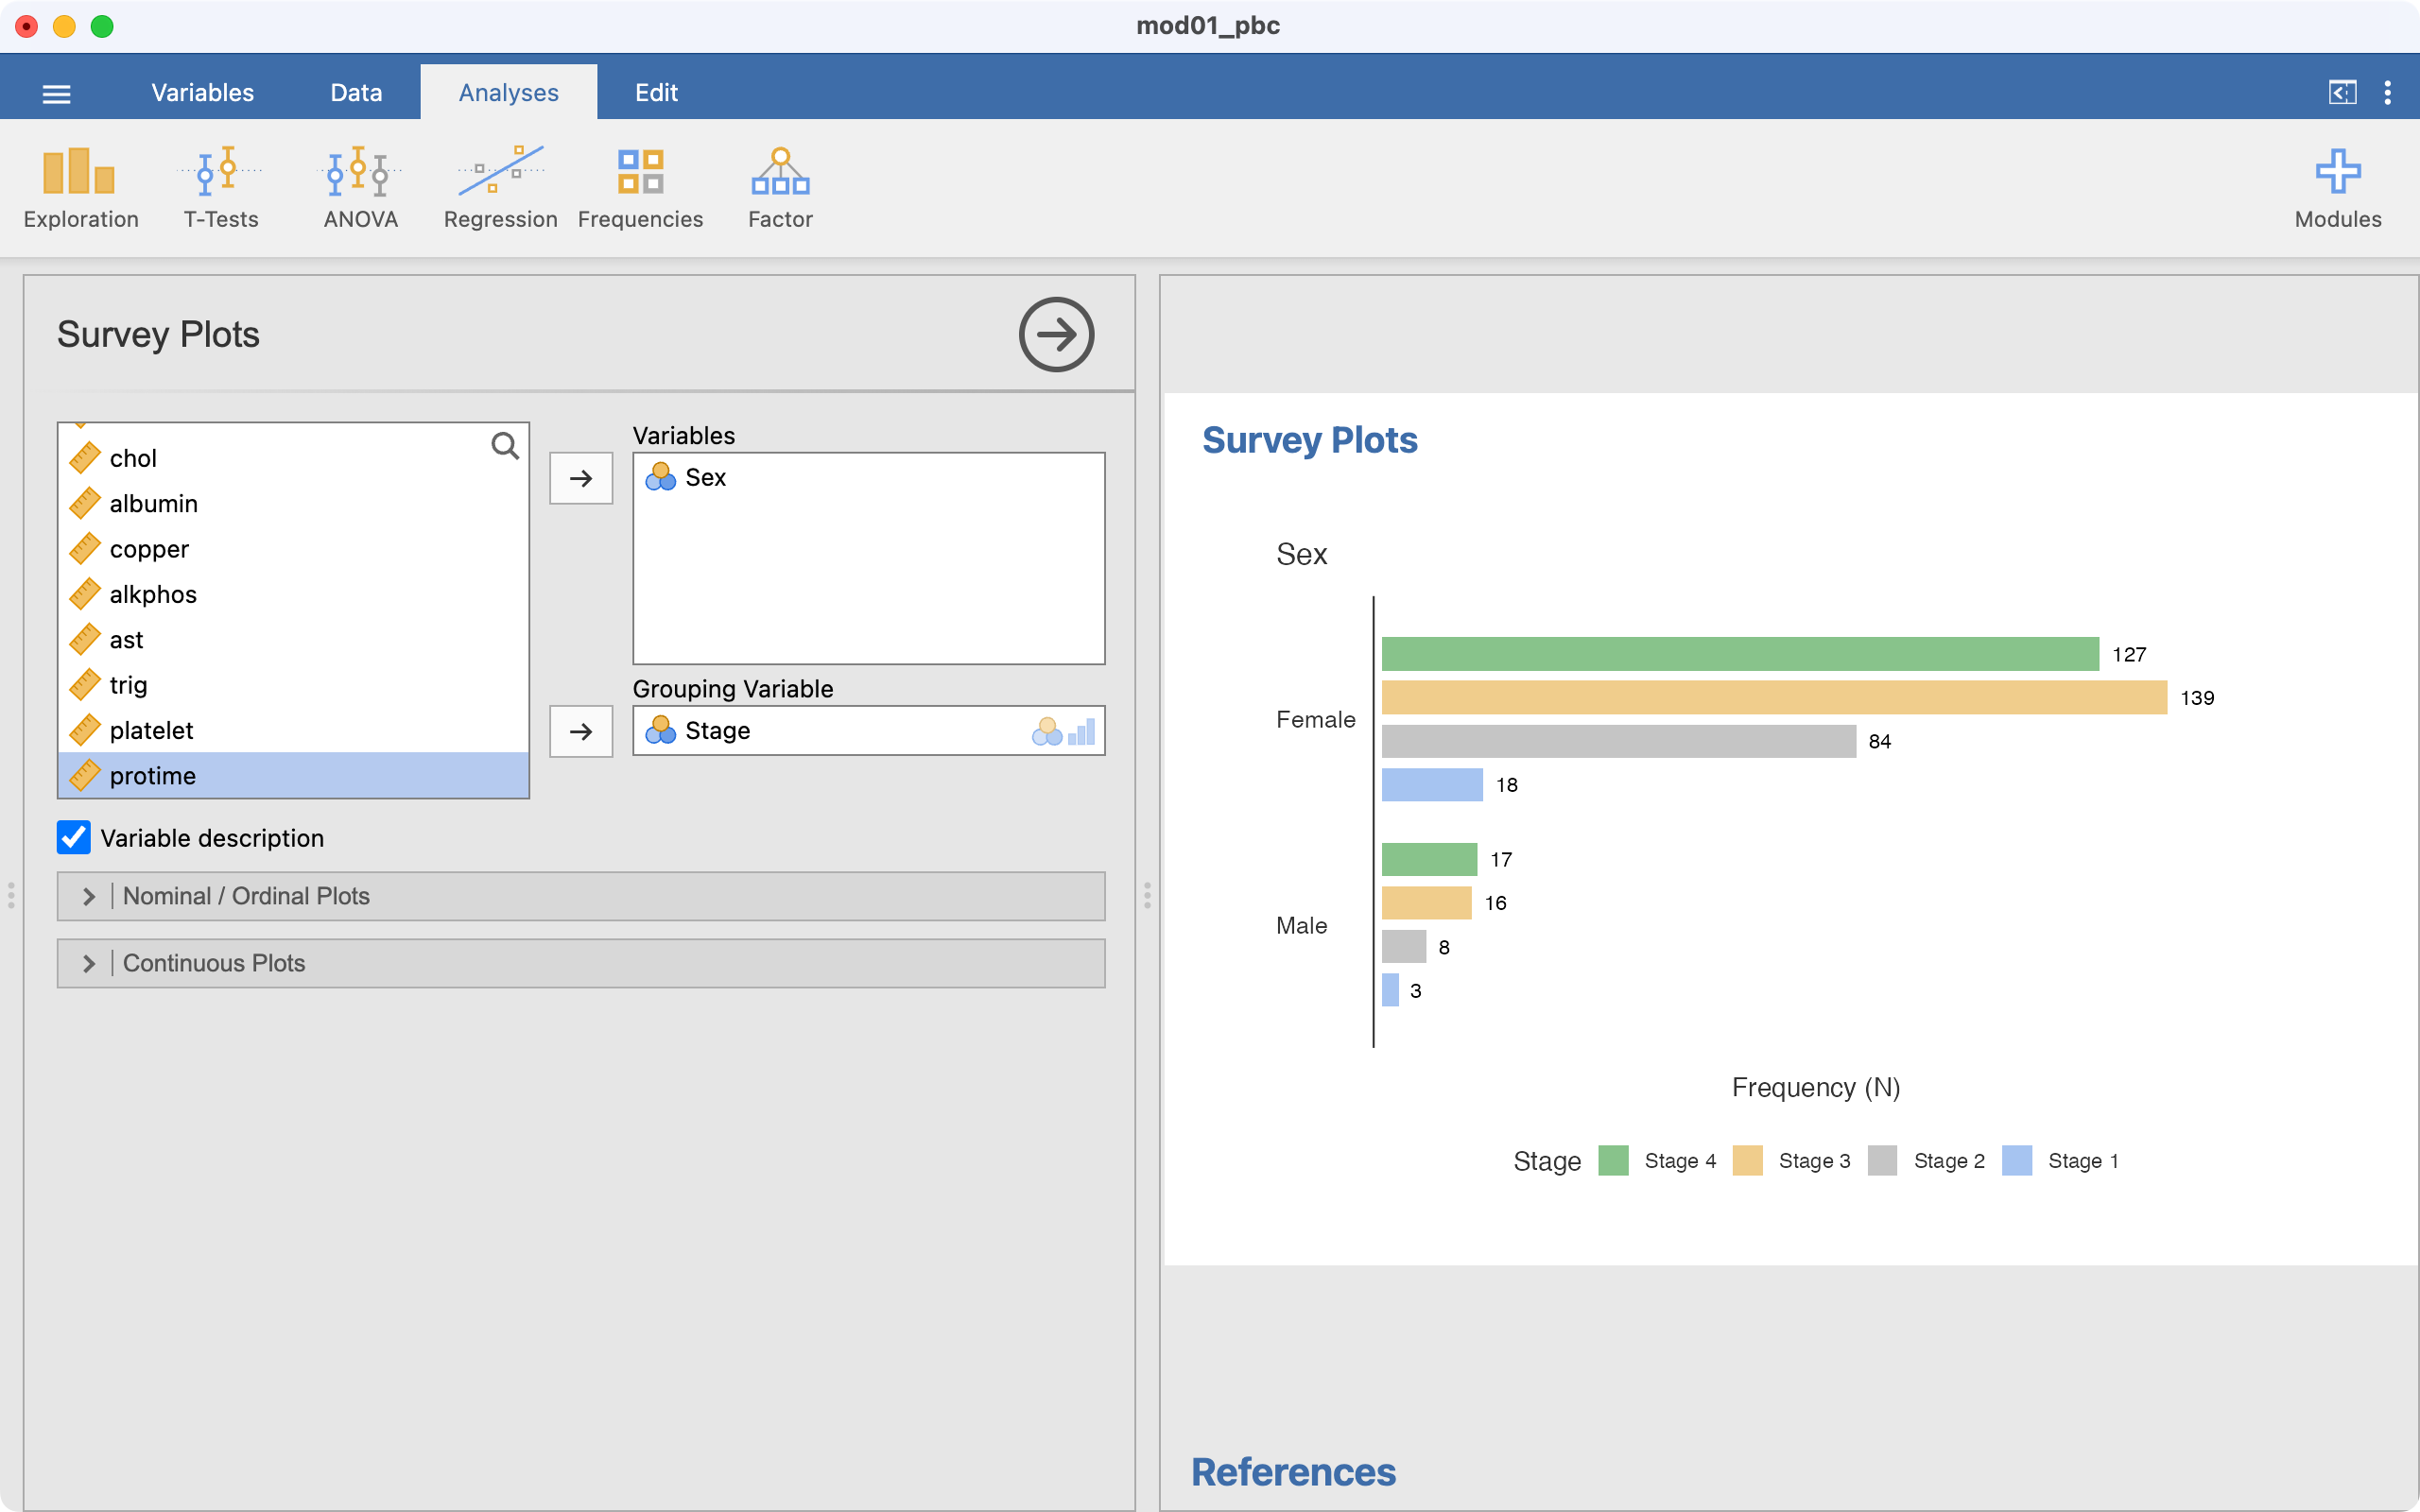
\includegraphics[keepaspectratio]{img/mod02/jamovi/surveymv-2.png}}

This has plotted a clustered bar chart, we want a stacked bar chart, so
select \textbf{Stacked bar}. Also, we want to plot percentages, not
counts, so choose \textbf{Percentages}:

\pandocbounded{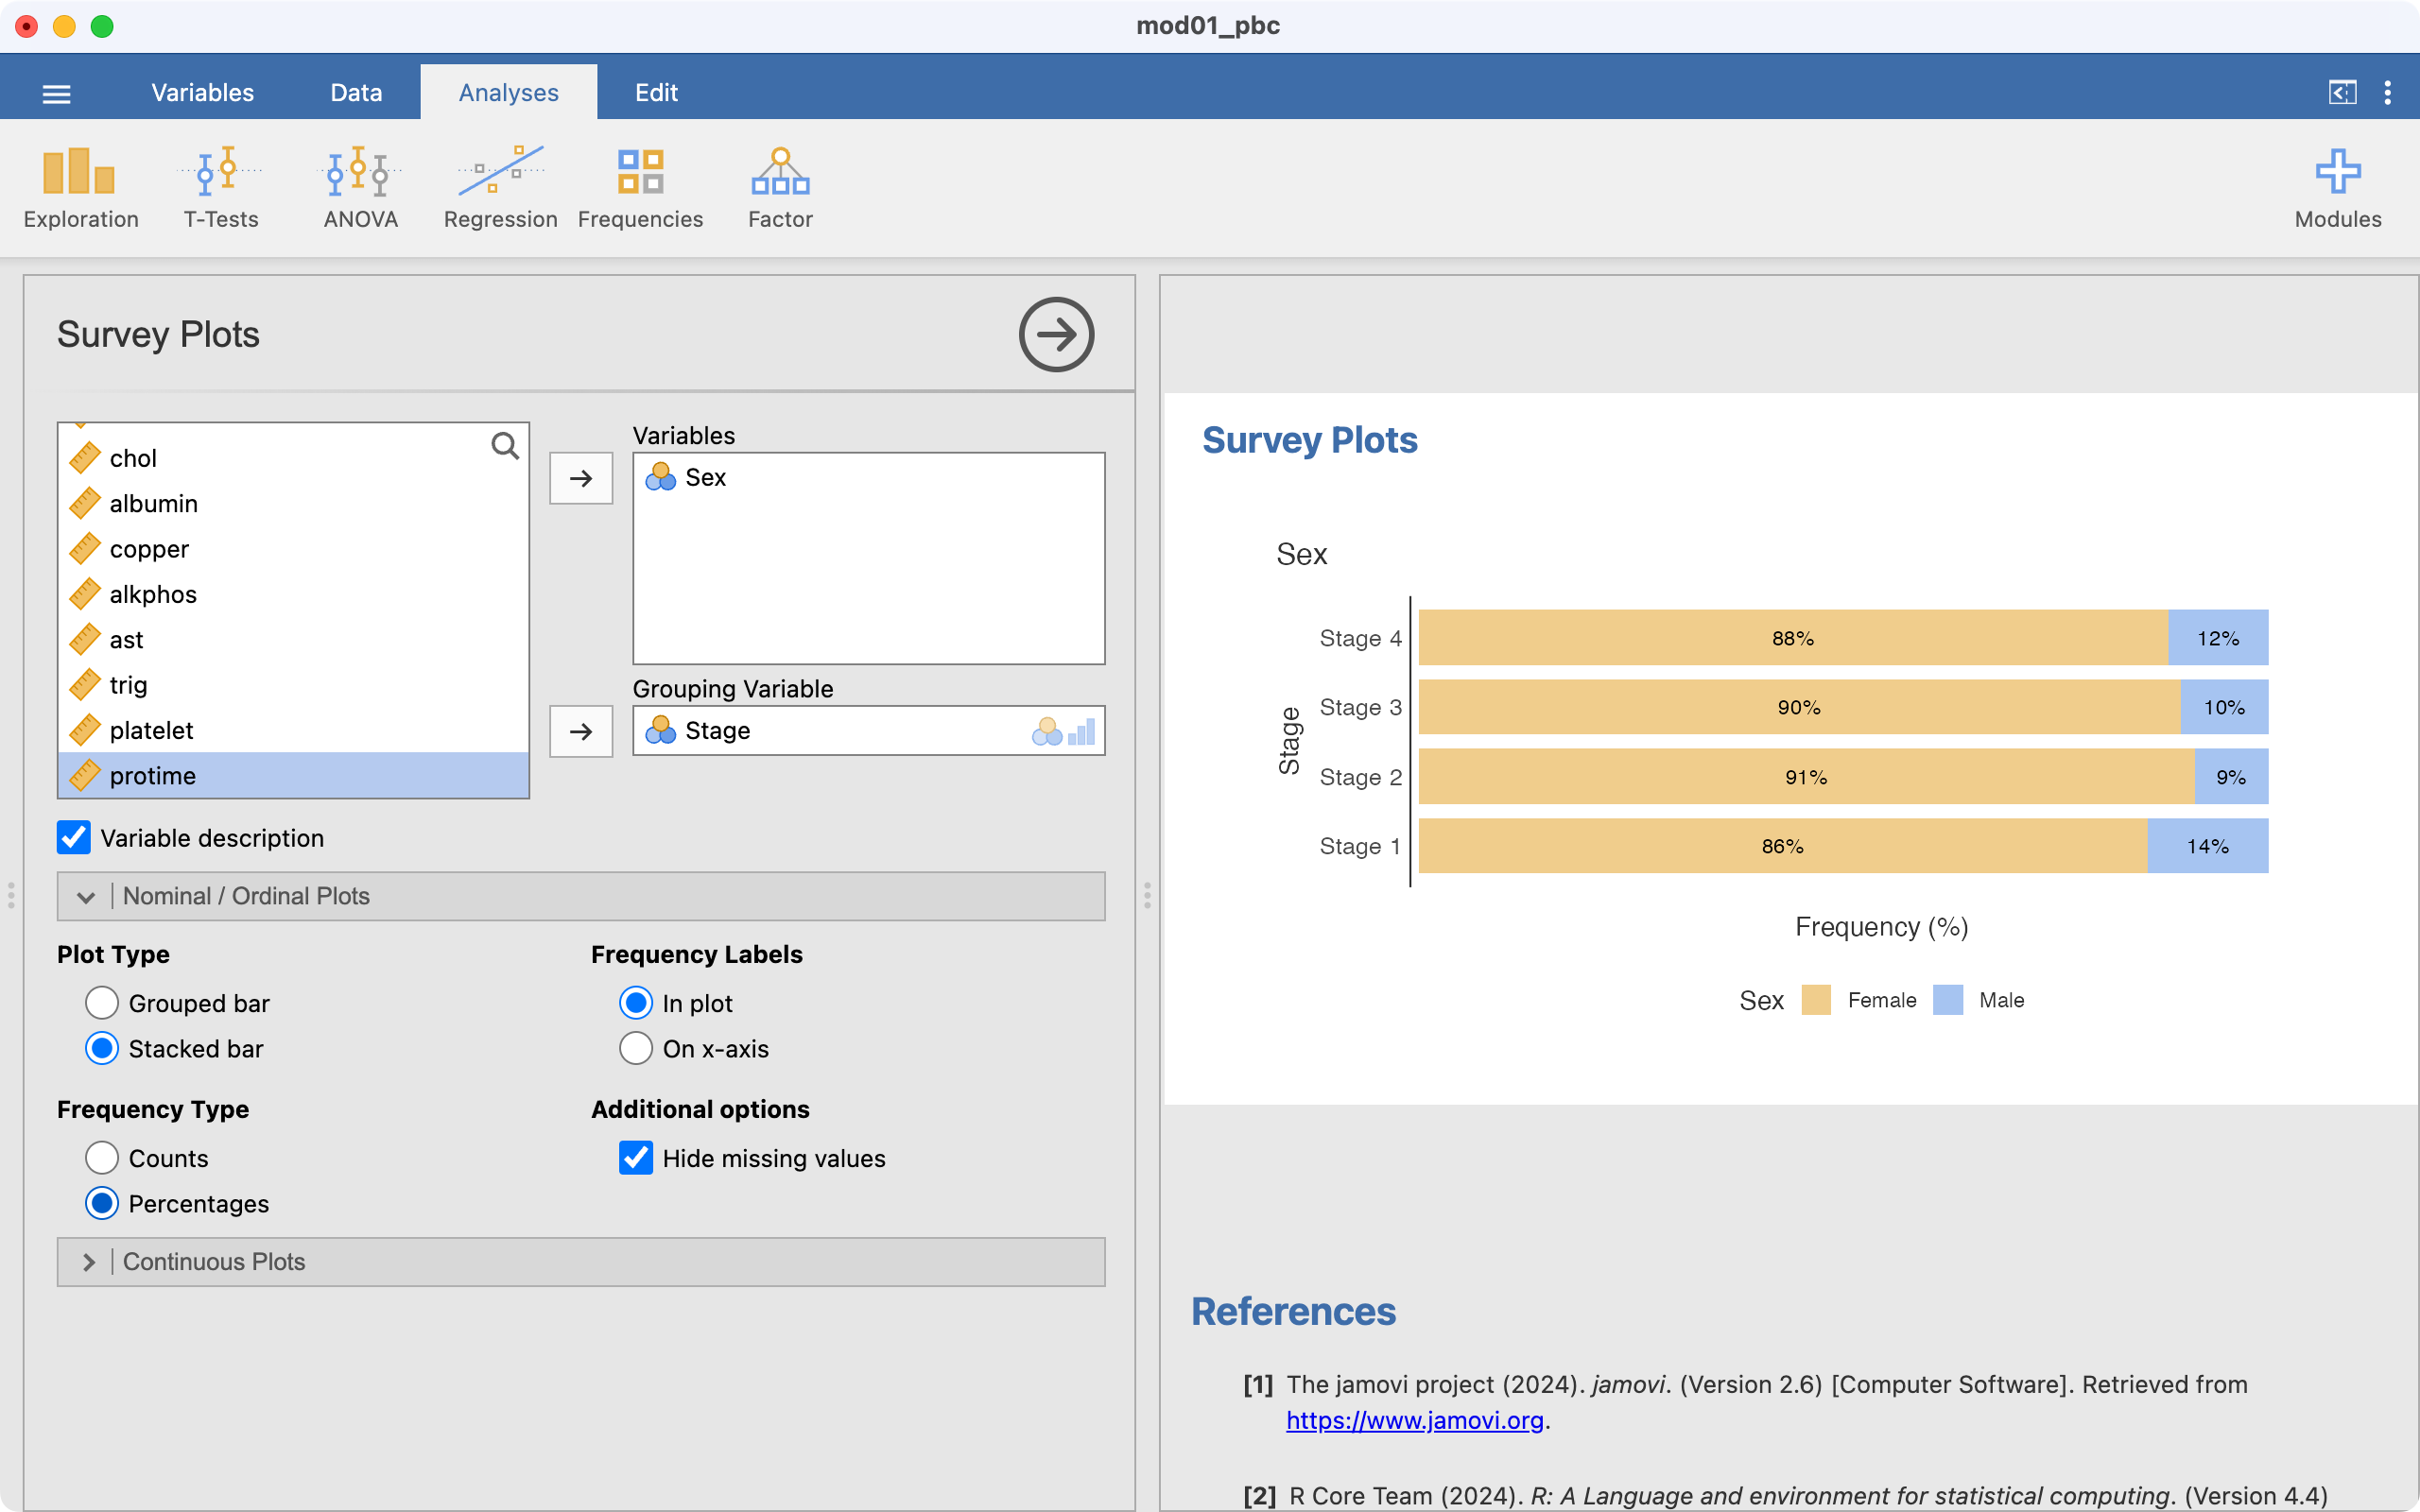
\includegraphics[keepaspectratio]{img/mod02/jamovi/surveymv-3.png}}

Our stacked relative frequency chart has been completed. While this
produces a bar chart with horizontal bars, it often performs better with
labelling of the groups than the previous method.

\section{Recoding data}\label{sec-recoding-data-jmv}

One task that is common in statistical computing is to recode variables.
For example, we might want to group some categories of a categorical
variable, or to present a continuous variable in a categorical way.

In this example, we can use the \texttt{pbc} data and recode age into
age groups:

\begin{itemize}
\tightlist
\item
  Less than 30
\item
  30 to less than 50
\item
  50 to less than 70
\item
  70 or older
\end{itemize}

Recoding can be done using \textbf{Data \textgreater{} Transform}.

First, click \textbf{Data} to view the spreadsheet, then click in an
empty column, then click \textbf{Setup \textgreater{} NEW TRANSFORMED
VARIABLE}. We need to specify three things:

\begin{enumerate}
\def\labelenumi{\arabic{enumi}.}
\tightlist
\item
  The name of the new variable. Here, we will choose
  \texttt{age\ group}.
\item
  The source variable. Here, we want to recode \textbf{from}
  \texttt{age}, so choose \texttt{age}.
\item
  The \texttt{transform}, which is where we define the rules of the
  recode. Choose \textbf{Create New Transform}.
\end{enumerate}

\pandocbounded{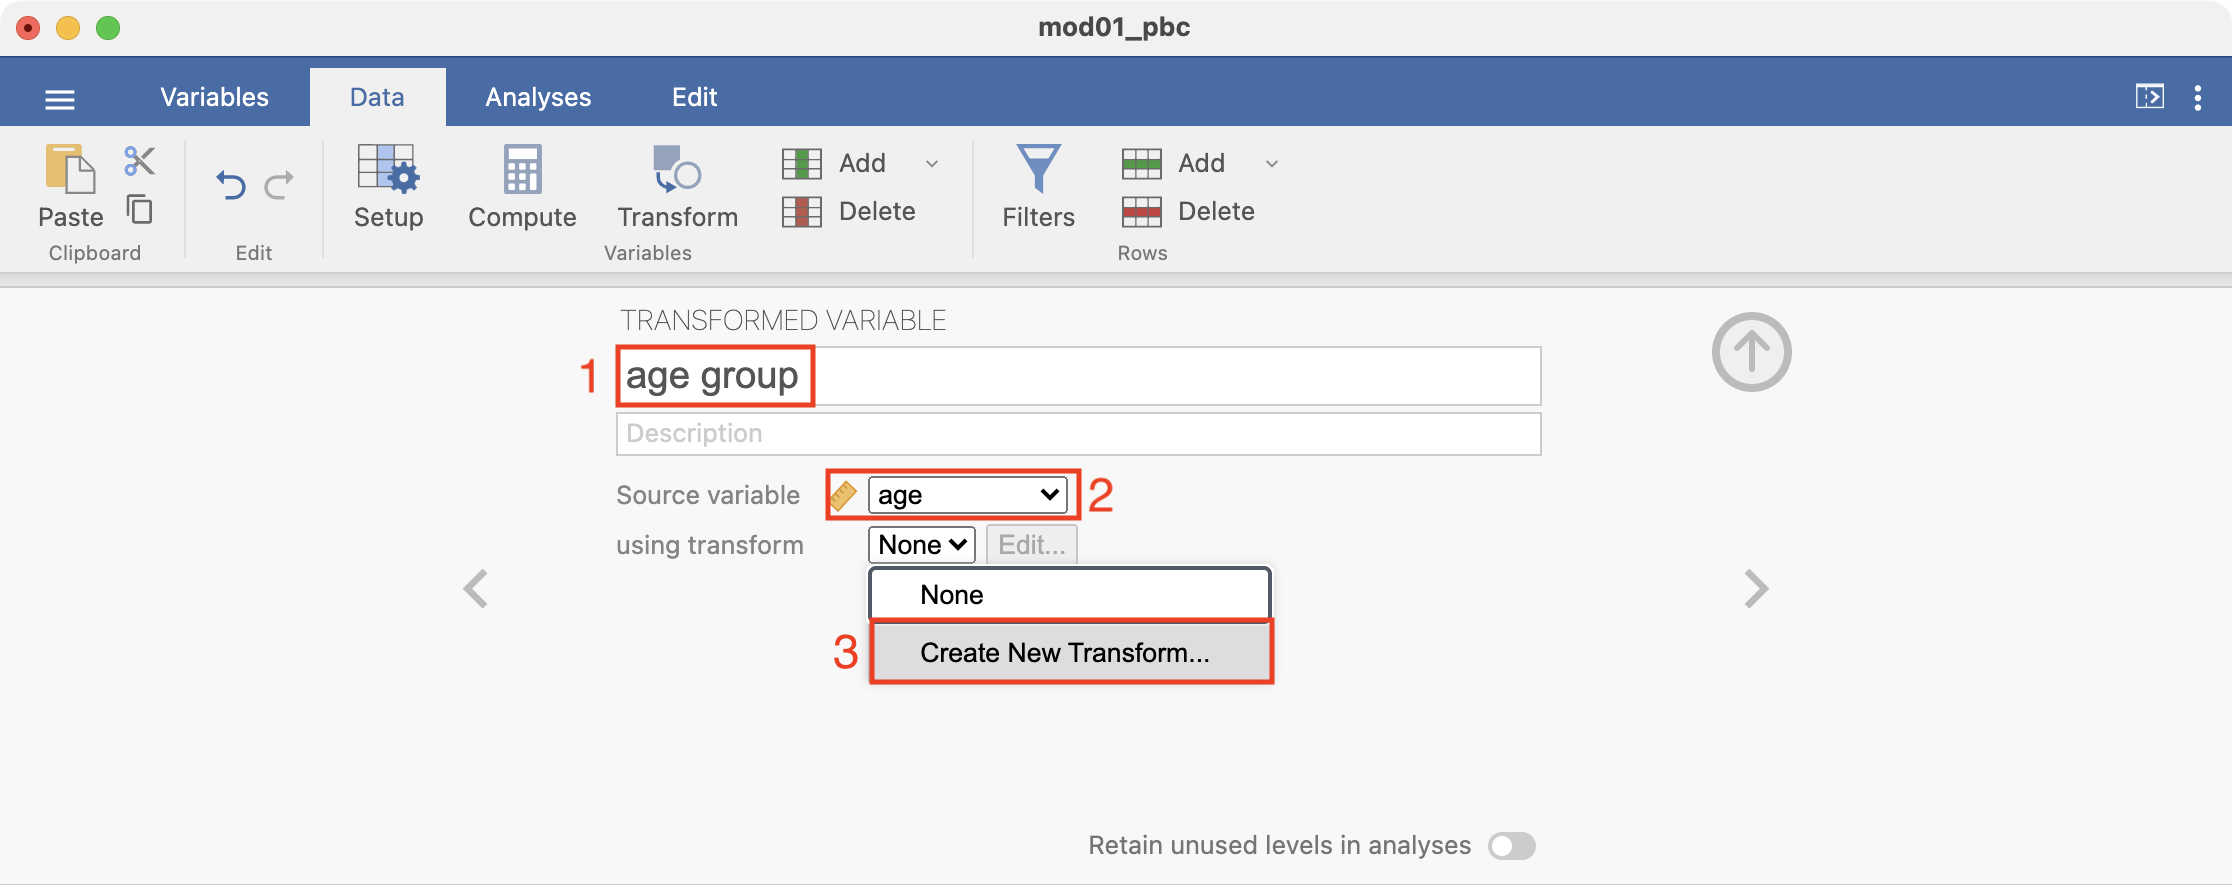
\includegraphics[keepaspectratio]{img/mod02/jamovi/mod02-recode2.png}}

The \texttt{transform} is built up by specifying the \textbf{recode
conditions}. Click \textbf{+ Add recode condition} to define the first
condition:

\pandocbounded{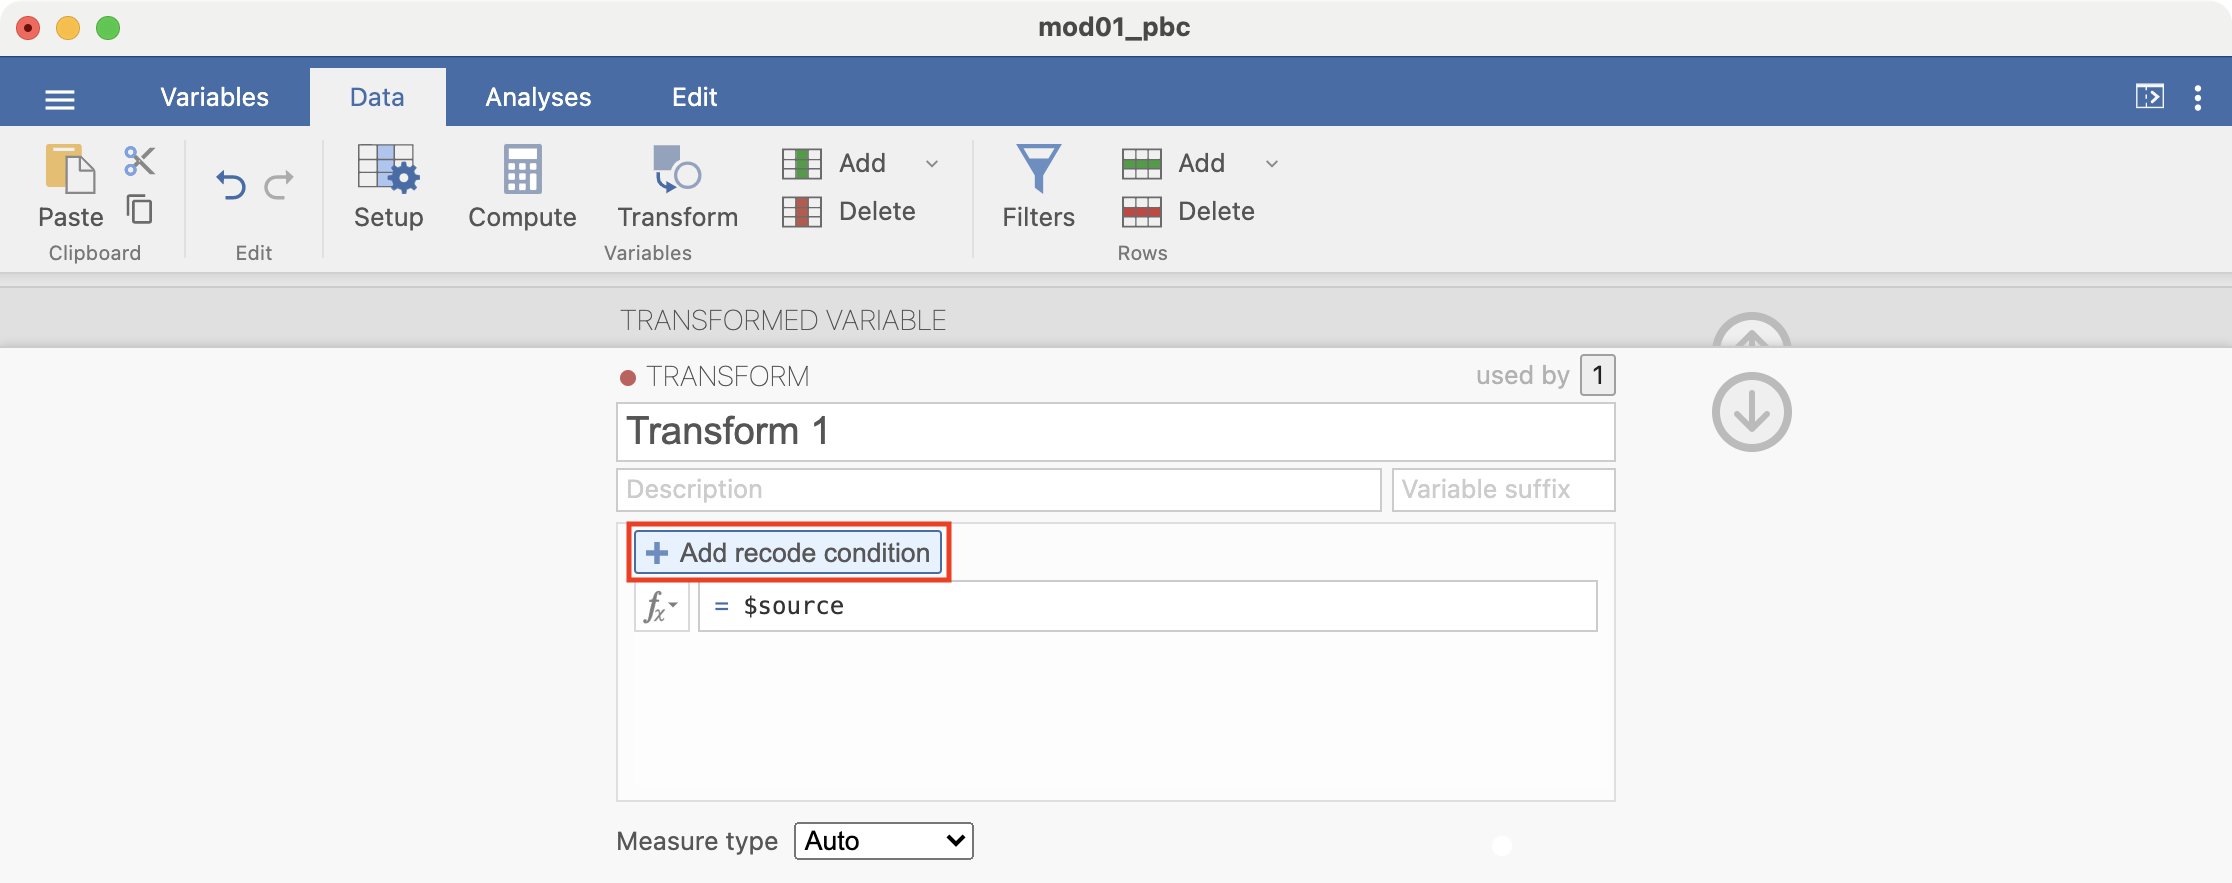
\includegraphics[keepaspectratio]{img/mod02/jamovi/mod02-recode3.png}}

Here we want to define all ages less than 30 as ``Less than 30''.
Complete the recode condition so it appears as:
\texttt{if\ \$source\ \textless{}\ 30\ use\ "Less\ than\ 30"}. Note that
the quotation marks around ``Less than 30'' are required:

\pandocbounded{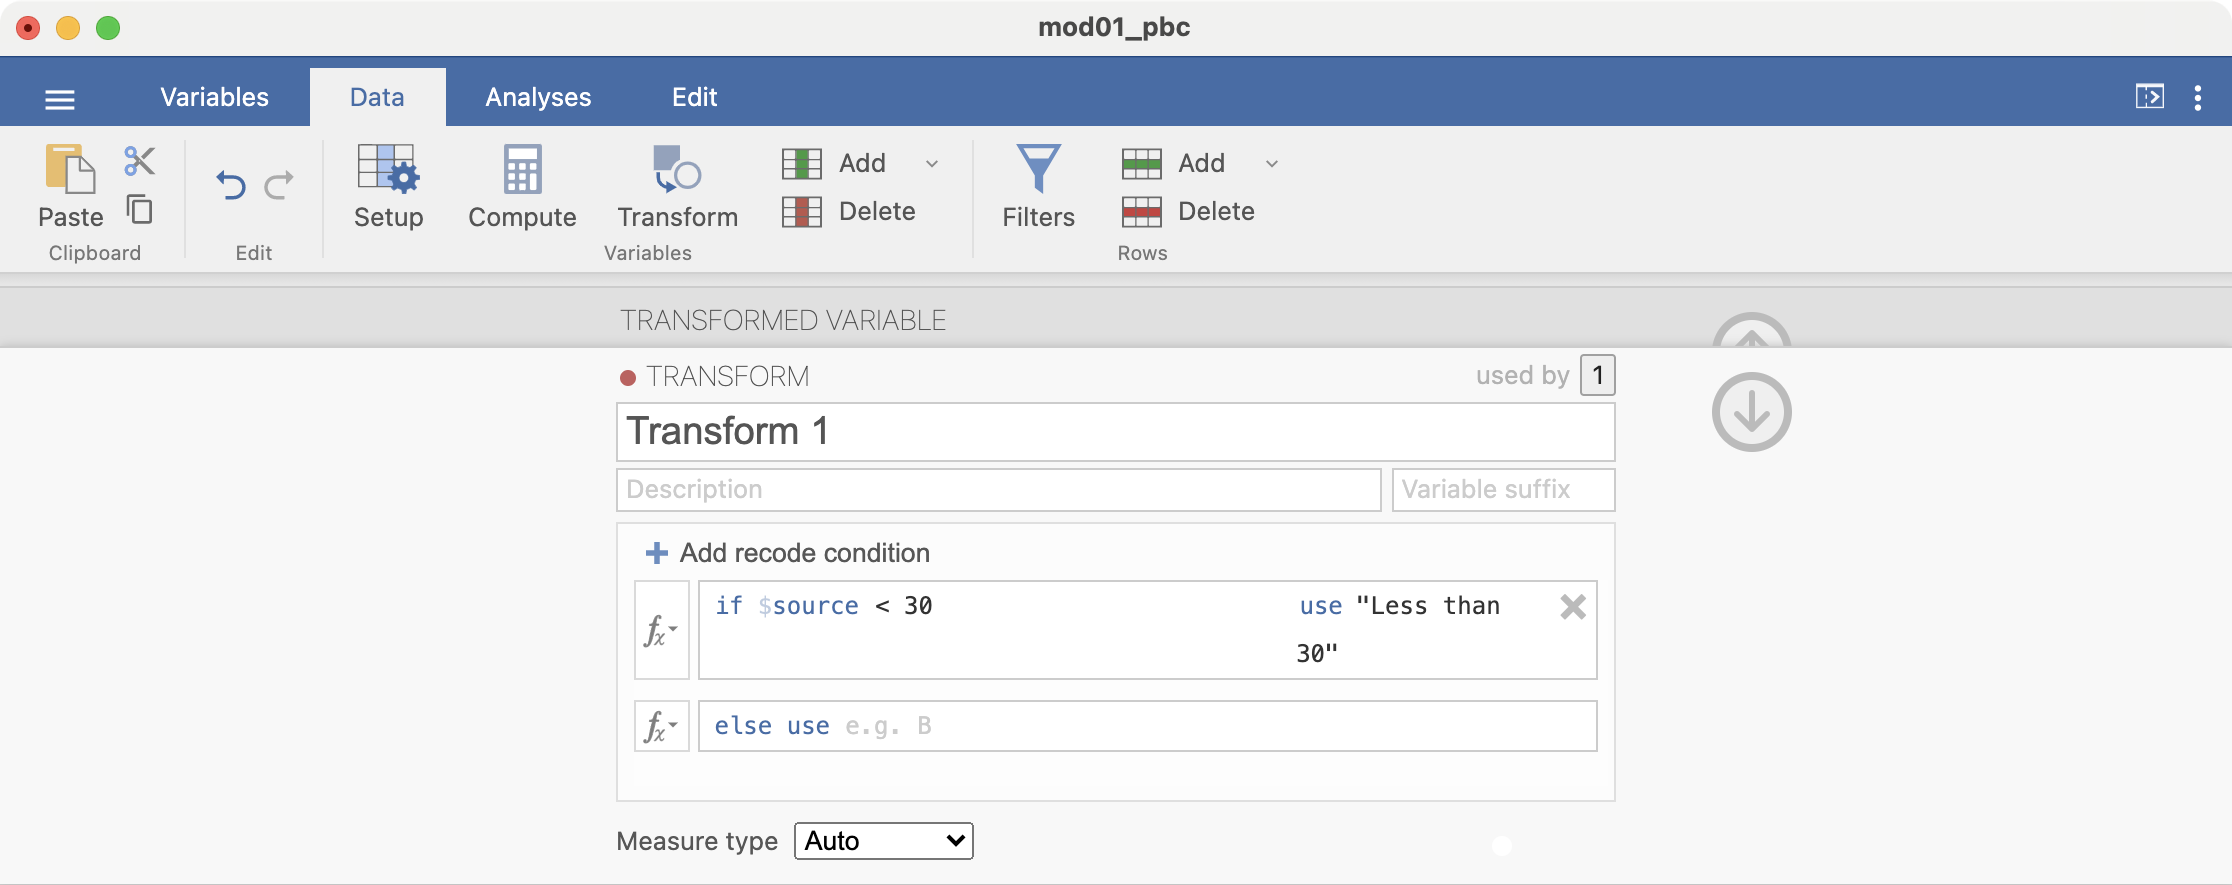
\includegraphics[keepaspectratio]{img/mod02/jamovi/mod02-recode4.png}}

Add another recode condition, which will be applied if the first
condition is not satisfied:
\texttt{if\ \$source\ \textless{}\ 50\ use\ "30\ to\ less\ than\ 50"}:

\pandocbounded{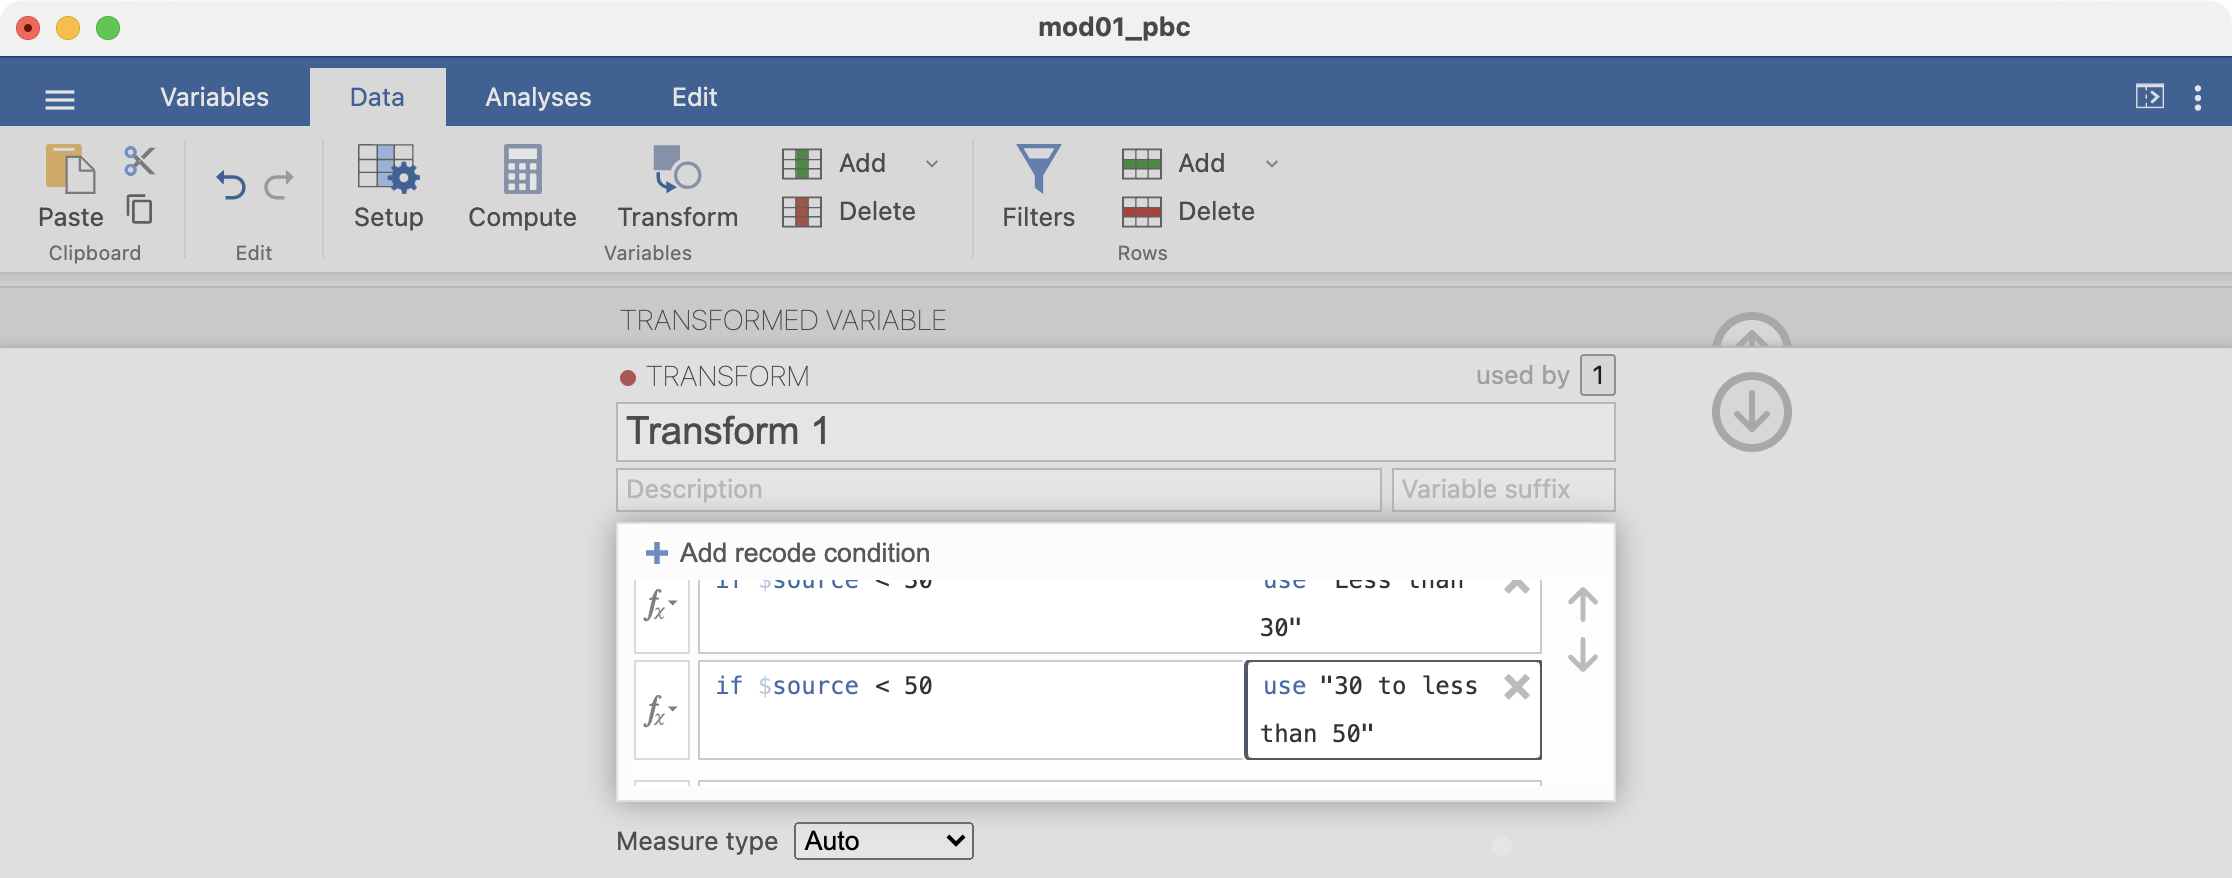
\includegraphics[keepaspectratio]{img/mod02/jamovi/mod02-recode5.png}}

Add another condition:
\texttt{if\ \$source\ \textless{}\ 70\ use\ "50\ to\ less\ than\ 70"}.
There is no need to add a condition for the final condition, simply
complete the final line: \texttt{else\ use\ "70\ or\ more"}:

\pandocbounded{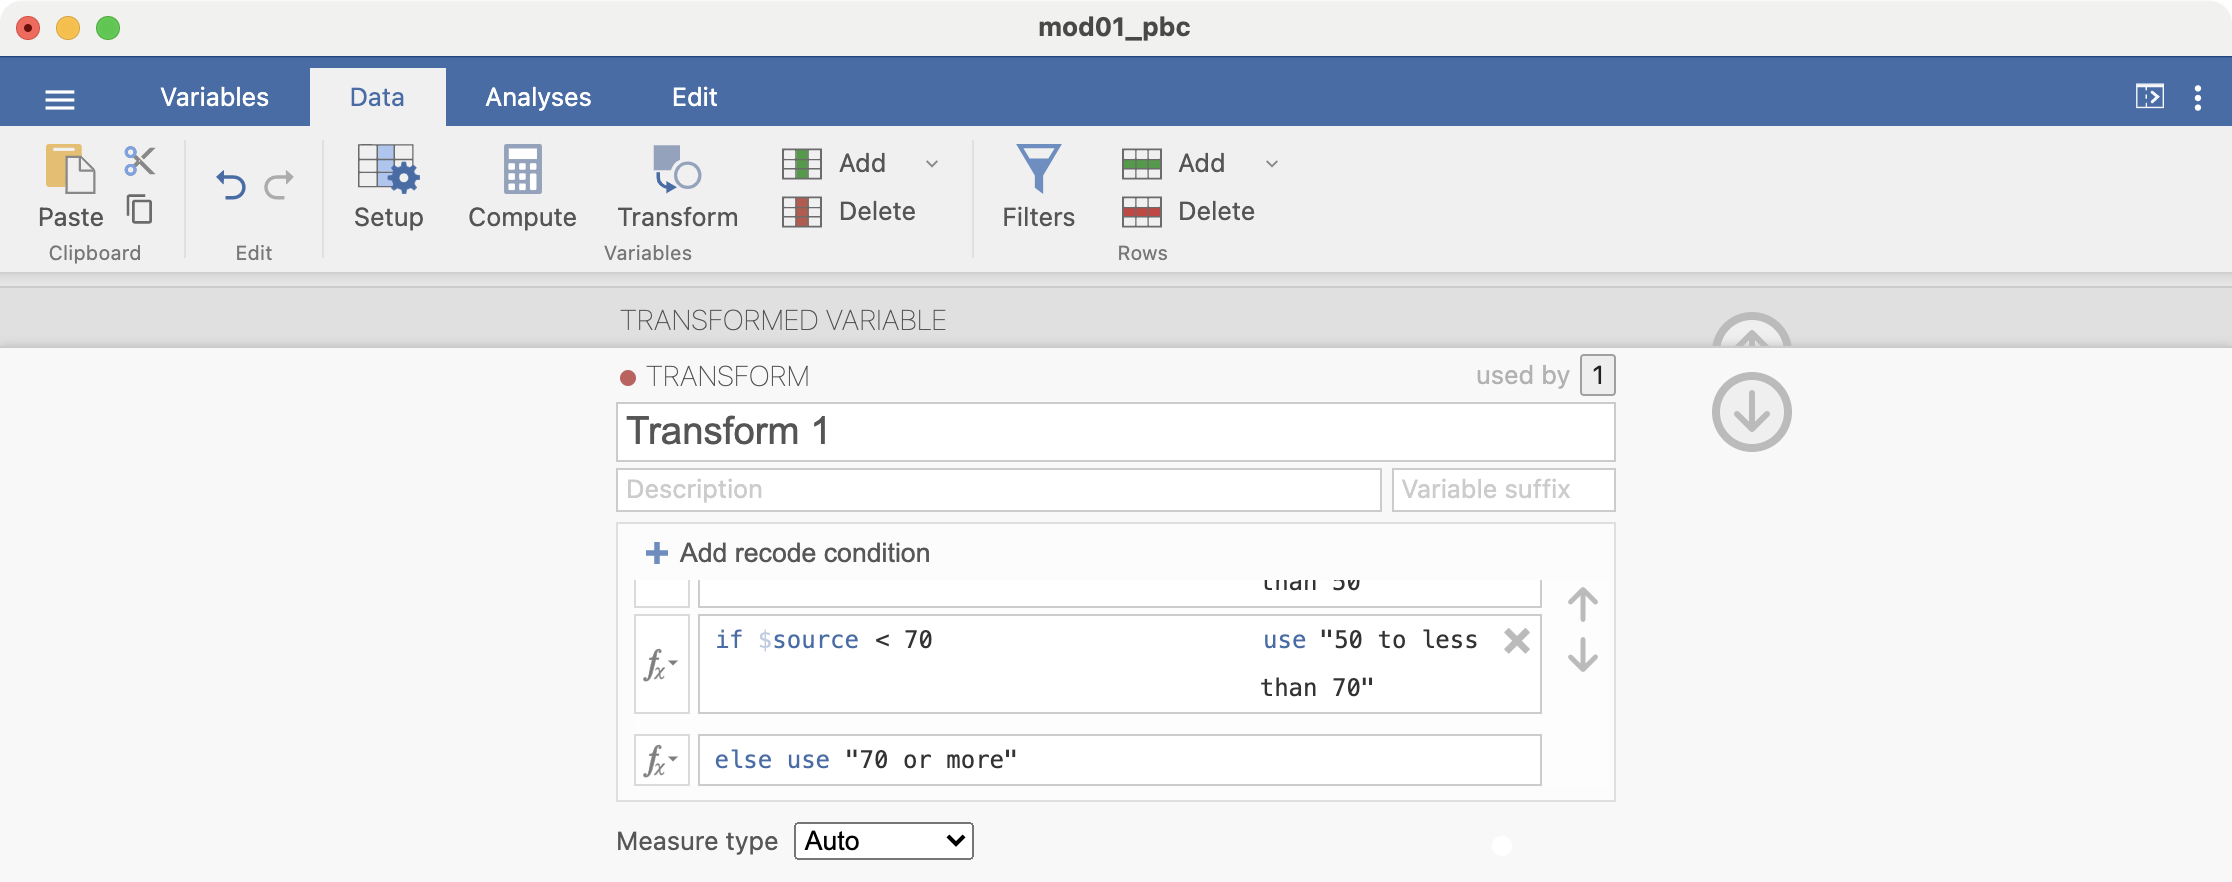
\includegraphics[keepaspectratio]{img/mod02/jamovi/mod02-recode6.png}}

Finally, click the \textbf{down} arrow to dismiss the transform builder,
and the \textbf{up} arrow to dismiss the transform dialog.

We can examine the new categories by obtaining a frequency table:
\textbf{Analyses \textgreater{} Exploration \textgreater{}
Descriptives}:

\pandocbounded{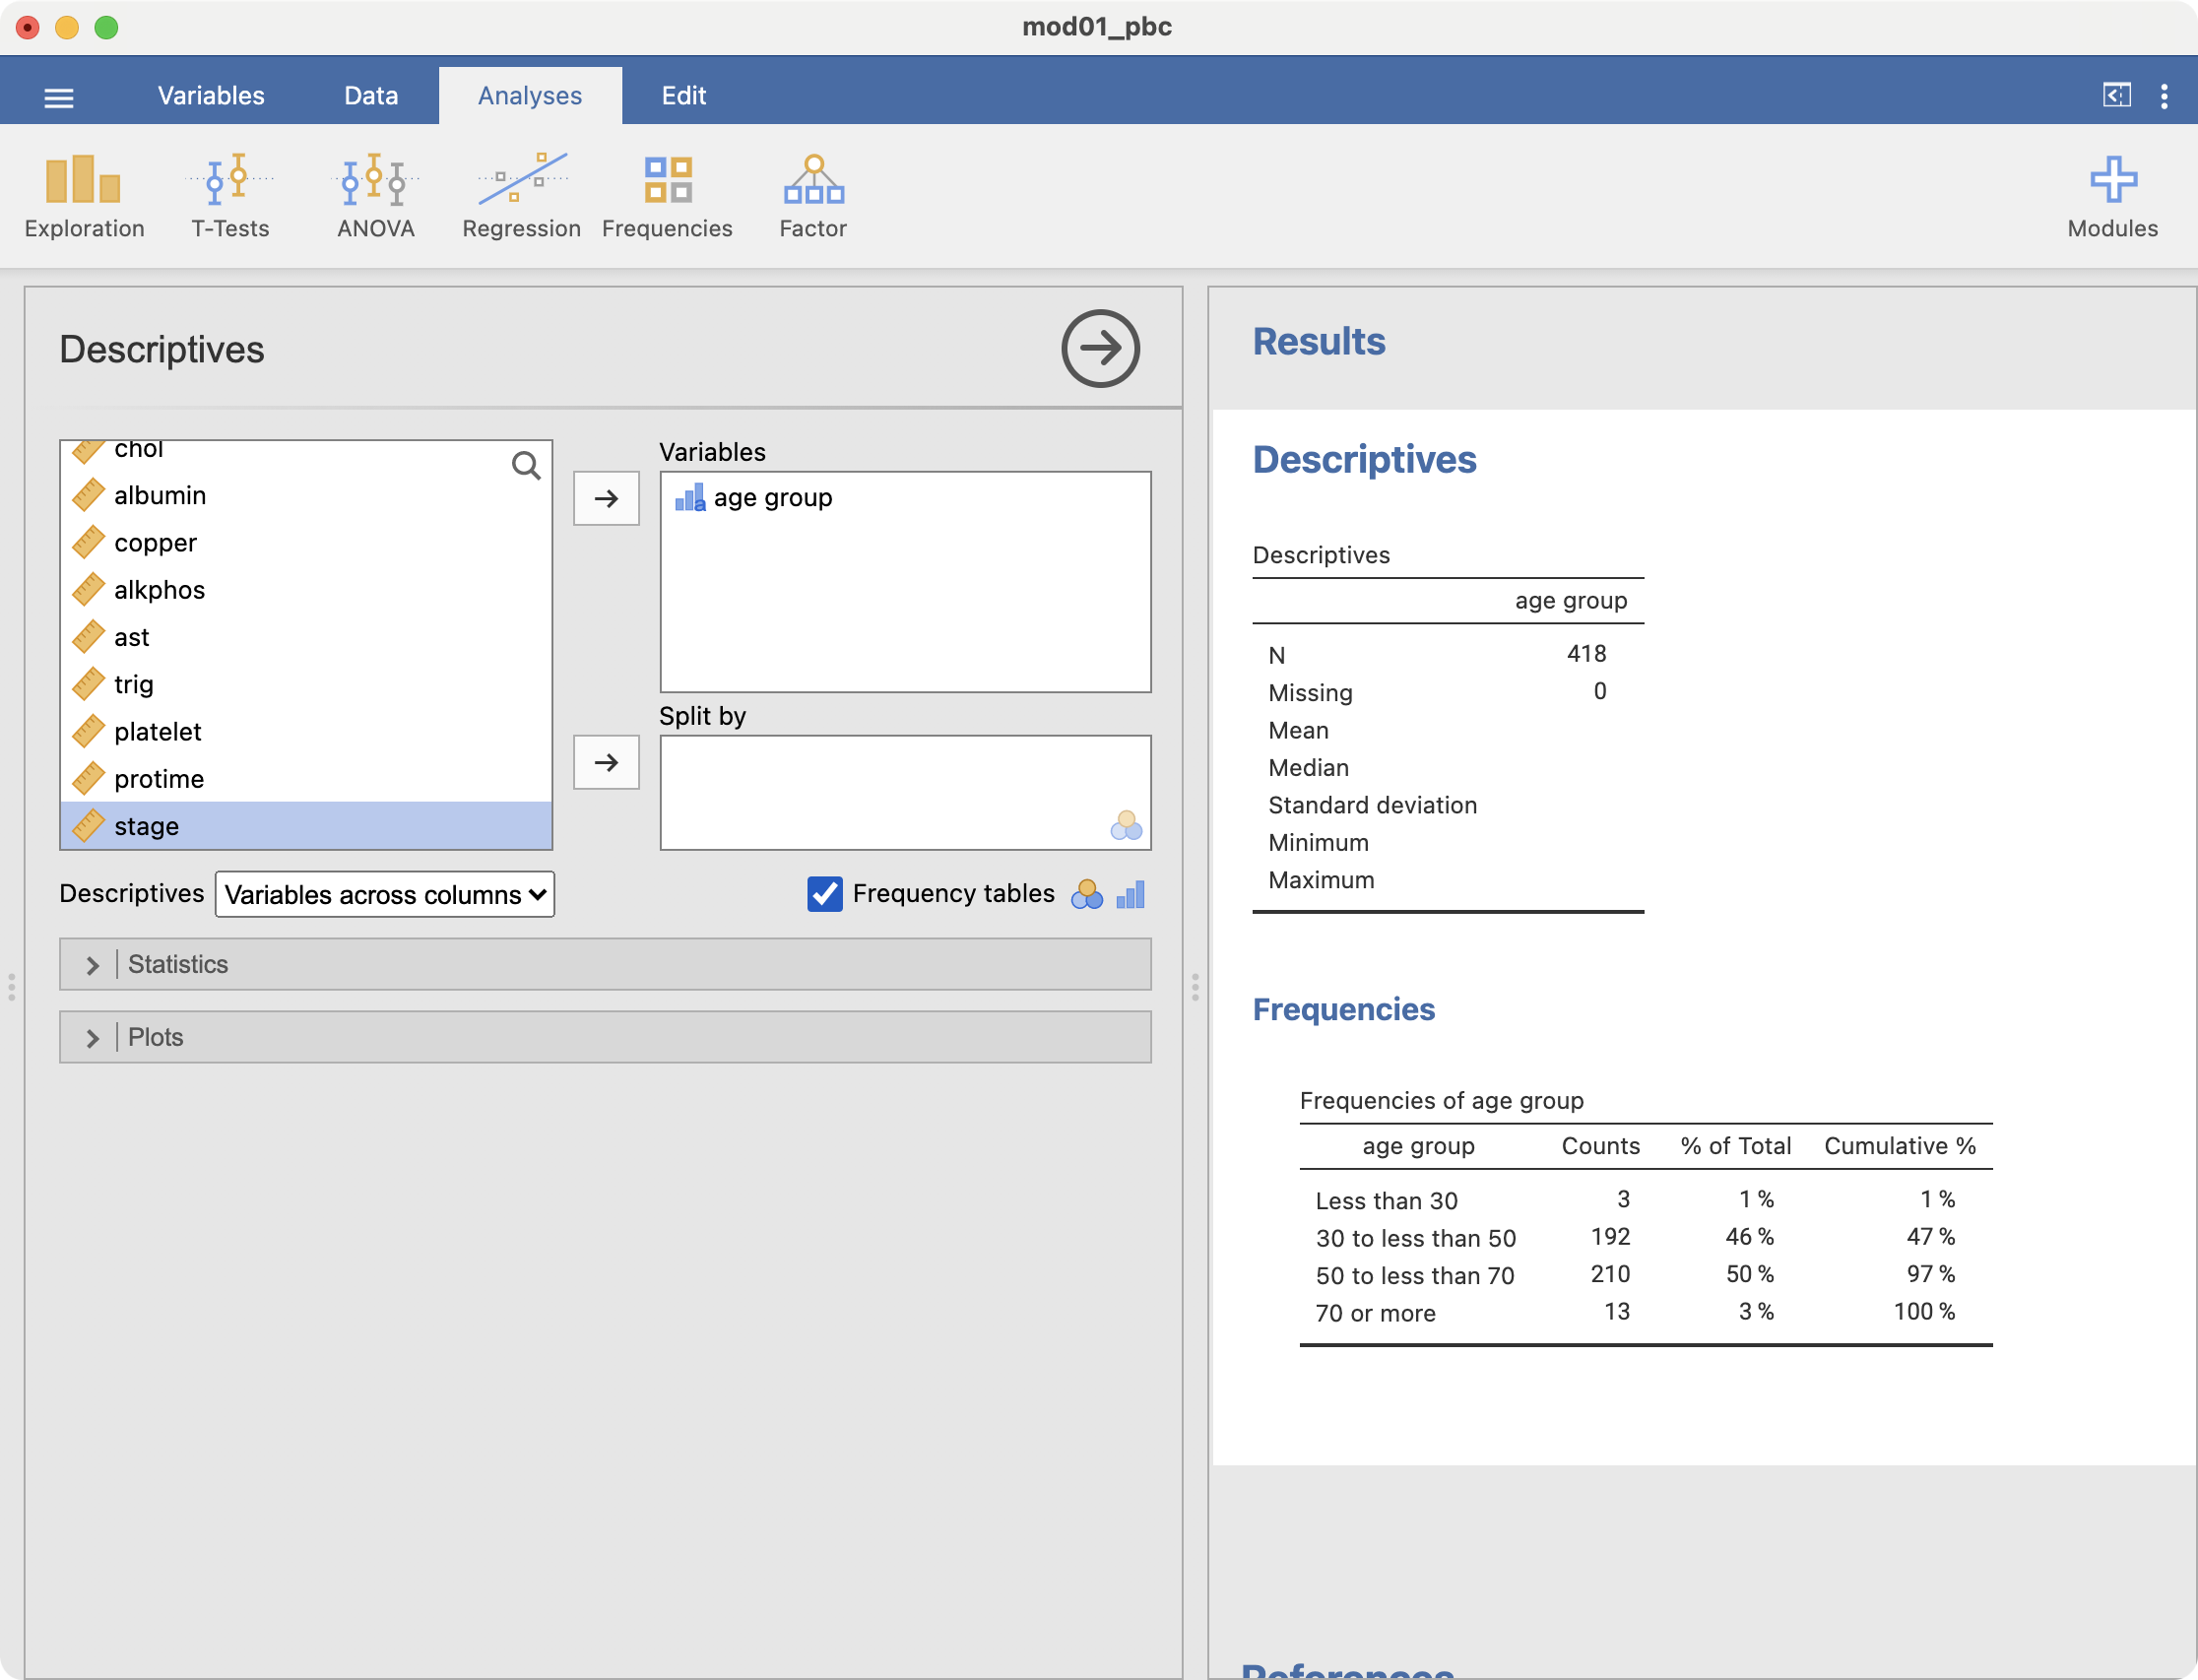
\includegraphics[keepaspectratio]{img/mod02/jamovi/mod02-recode7.png}}

\section{Computing binomial
probabilities}\label{computing-binomial-probabilities}

jamovi does not have a point-and-click method for computing
probabilities from a binomial distribution. Here, instructions are
provided for using a third-party applet. This Binomial Distribution
Applet has been posted at
\url{https://mabognar.github.io/apps/bin.html}, and provides a simple
and intuitive way to compute probabilities from a binomial distribution.

The applet requires three pieces of information:

\begin{itemize}
\tightlist
\item
  \(n\): the number of binary trials being considered
\item
  \(p\): the probability of ``success'' in each trial
\item
  \(x\): the number of success we are interested in
\end{itemize}

We also need to consider whether we are interested in the probability
being equal to, greater than, or less than x.

To do the computation for part (a) in Worked Example 2.1:

\begin{itemize}
\tightlist
\item
  \(x\) is the number of successes, here, the number of smokers
  (i.e.~x=3);
\item
  \(n\) is the number of trials (i.e.~n=6);
\item
  and \(p\) is probability of drawing a smoker from the population,
  which is 19.8\% (i.e.~p=0.198).
\end{itemize}

Replace each of these with the appropriate number into the applet:

\pandocbounded{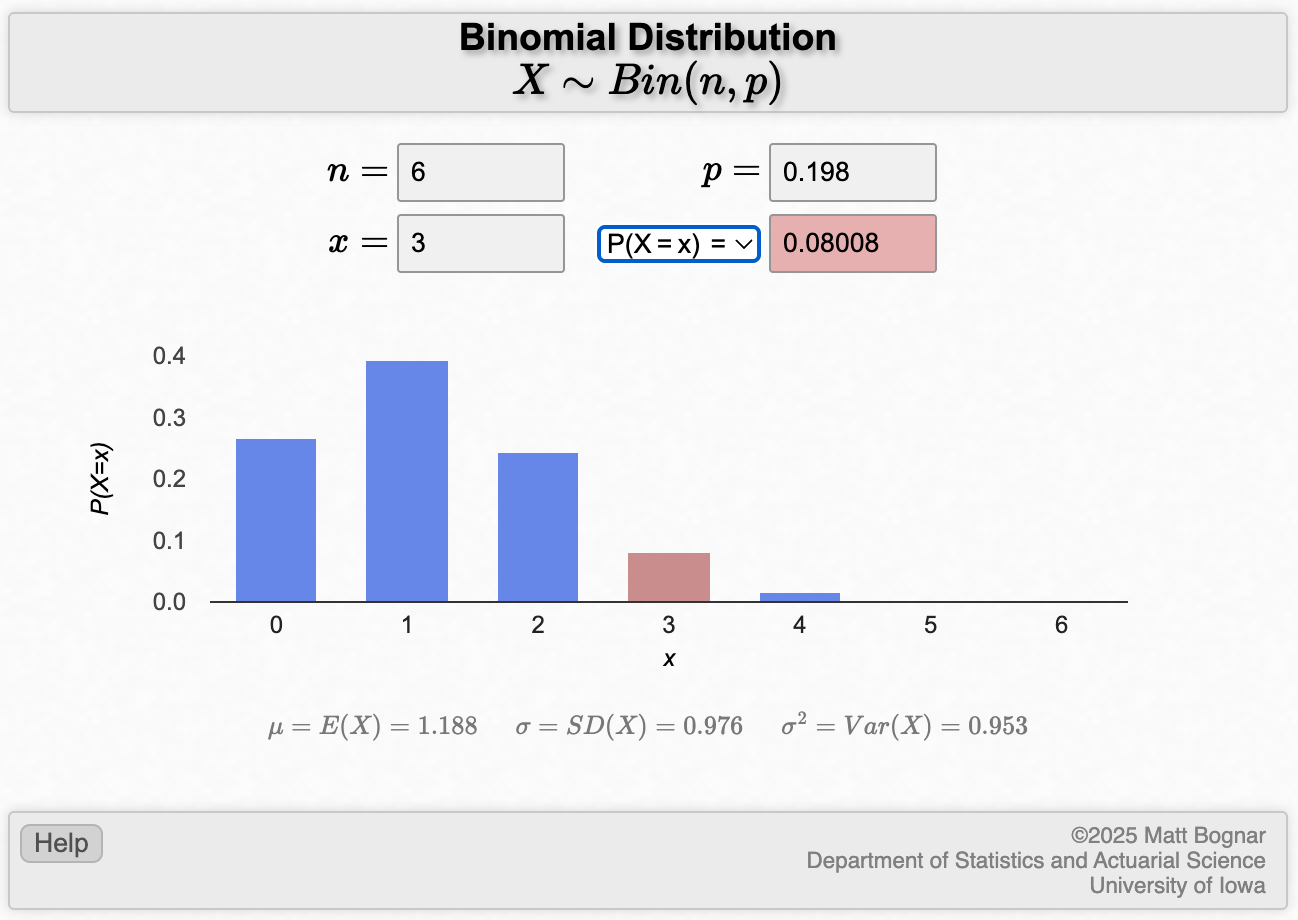
\includegraphics[keepaspectratio]{img/mod02/jamovi/mod02-bin-01.png}}

To calculate the probability of at least 4 smokers in part (b), we
change the drop-down to ``P(X≥x)'', and x to be equal to 4:

\pandocbounded{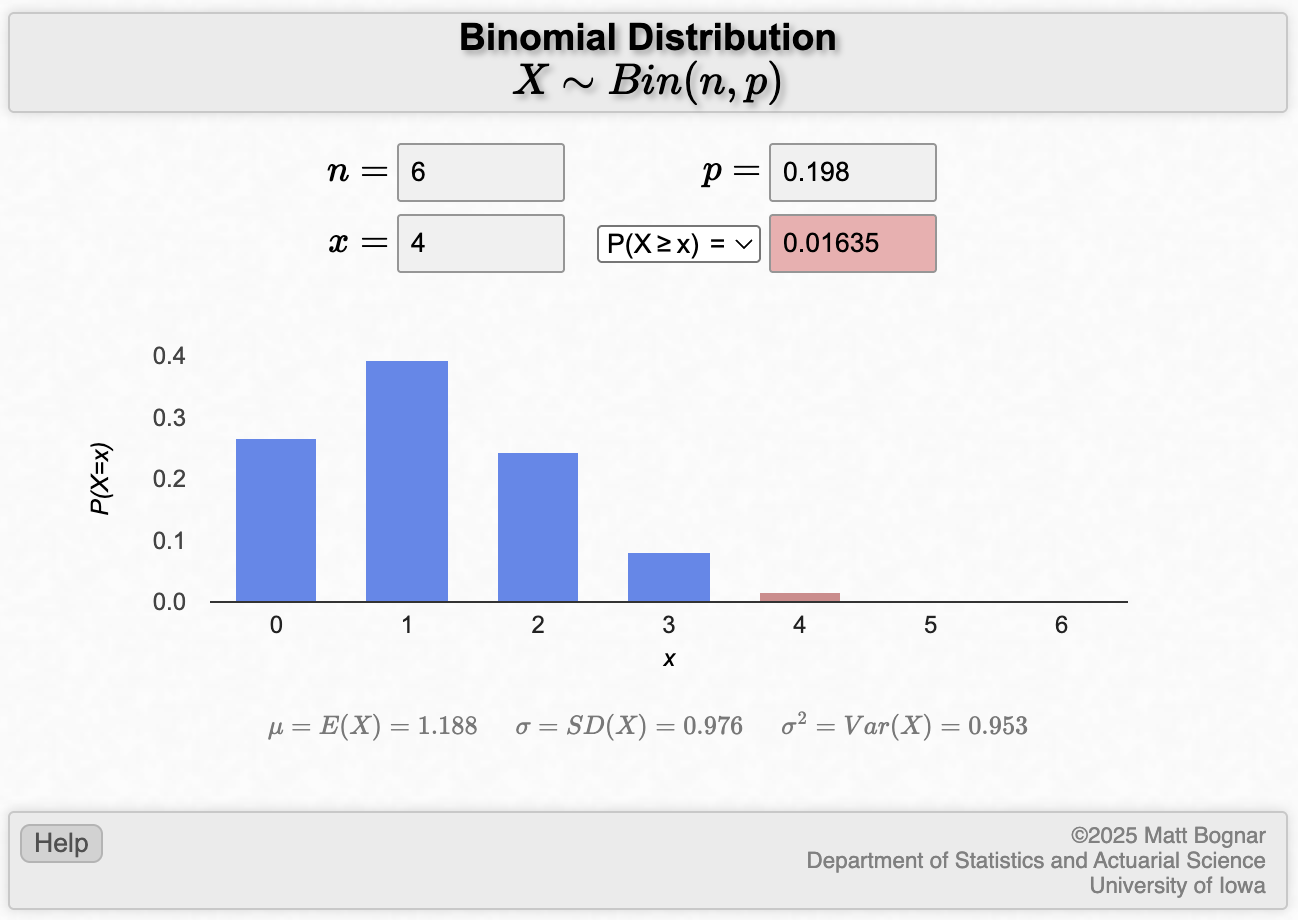
\includegraphics[keepaspectratio]{img/mod02/jamovi/mod02-bin-02.png}}

To calculate the probability of at most 2 smokers part (c), we we change
the drop-down to ``P(X≤x)'', and x to be equal to 2:

\pandocbounded{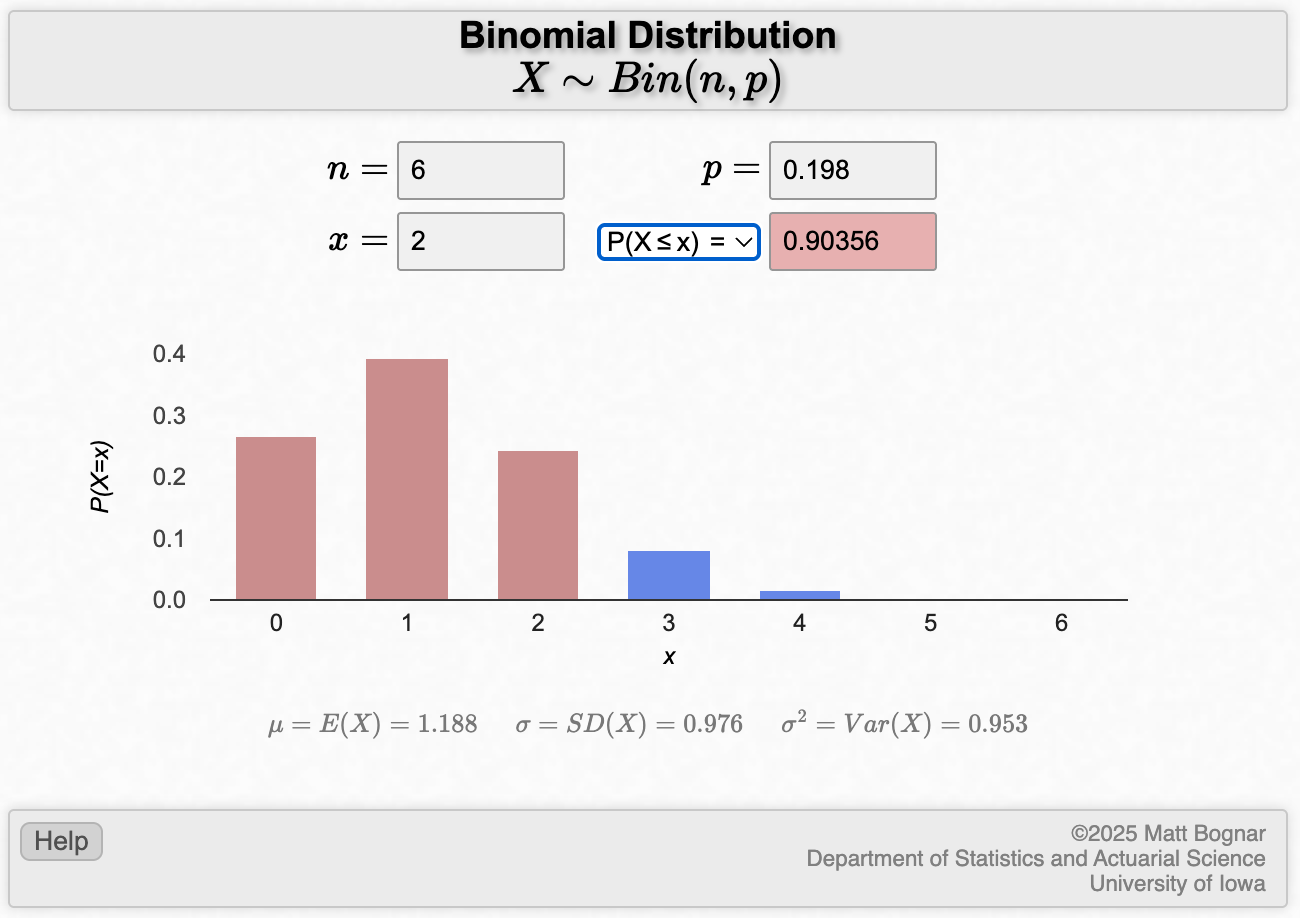
\includegraphics[keepaspectratio]{img/mod02/jamovi/mod02-bin-03.png}}

\newpage{}

\bookmarksetup{startatroot}

\chapter*{R notes}\label{r-notes}
\addcontentsline{toc}{chapter}{R notes}

\markboth{R notes}{R notes}

\subsection{Producing a one-way frequency
table}\label{producing-a-one-way-frequency-table-1}

We have three categorical variables to summarise in our PBC Table 1:
sex, stage and vital status. These variables are best summarised using
one-way frequency tables, which can be constructed using the
\texttt{descriptives} function from the \texttt{jmv} package, with the
\texttt{freq\ =\ TRUE} option. Before constructing frequency tables
however, we \emph{must define the variables as categorical variables},
by converting them to \emph{factors}.

\subsubsection{Defining categorical variables as
factors}\label{sec-cat-as-factors}

To define a categorical variable as such in R, we define it as a
\textbf{factor} using the factor function:

\texttt{factor(variable=,\ levels=,\ labels=)}

We specify:

\begin{itemize}
\tightlist
\item
  levels: the values the categorical variable can take
\item
  labels: the labels corresponding to each of the levels (entered in the
  same order as the levels)
\end{itemize}

To define our variable \texttt{sex} as a factor, we use:

\begin{Shaded}
\begin{Highlighting}[]
\NormalTok{pbc }\OtherTok{\textless{}{-}} \FunctionTok{readRDS}\NormalTok{(}\StringTok{"data/activities/mod01\_pbc.rds"}\NormalTok{)}

\NormalTok{pbc}\SpecialCharTok{$}\NormalTok{sex }\OtherTok{\textless{}{-}} \FunctionTok{factor}\NormalTok{(pbc}\SpecialCharTok{$}\NormalTok{sex, }\AttributeTok{levels =} \FunctionTok{c}\NormalTok{(}\DecValTok{1}\NormalTok{, }\DecValTok{2}\NormalTok{), }\AttributeTok{labels =} \FunctionTok{c}\NormalTok{(}\StringTok{"Male"}\NormalTok{, }\StringTok{"Female"}\NormalTok{))}
\end{Highlighting}
\end{Shaded}

We can then produce a frequency table:

\begin{Shaded}
\begin{Highlighting}[]
\FunctionTok{descriptives}\NormalTok{(}\AttributeTok{data =}\NormalTok{ pbc, }\AttributeTok{vars =}\NormalTok{ sex, }\AttributeTok{freq =} \ConstantTok{TRUE}\NormalTok{)}
\end{Highlighting}
\end{Shaded}

\begin{verbatim}

 DESCRIPTIVES

 Descriptives                  
 ───────────────────────────── 
                         sex   
 ───────────────────────────── 
   N                     418   
   Missing                 0   
   Mean                        
   Median                      
   Standard deviation          
   Minimum                     
   Maximum                     
 ───────────────────────────── 


 FREQUENCIES

 Frequencies of sex                                 
 ────────────────────────────────────────────────── 
   sex       Counts    % of Total    Cumulative %   
 ────────────────────────────────────────────────── 
   Male          44      10.52632        10.52632   
   Female       374      89.47368       100.00000   
 ────────────────────────────────────────────────── 
\end{verbatim}

\begin{quote}
Task: define \texttt{stage} and \texttt{status} (Vital Status) as
factors, and produce one-way frequency tables. Refer to the file
\texttt{pbc\_info.txt} to view the labels for each variable. For
example, for Stage:
\end{quote}

\begin{Shaded}
\begin{Highlighting}[]
\NormalTok{pbc}\SpecialCharTok{$}\NormalTok{stage }\OtherTok{\textless{}{-}} \FunctionTok{factor}\NormalTok{(}
\NormalTok{  pbc}\SpecialCharTok{$}\NormalTok{stage,}
  \AttributeTok{levels =} \FunctionTok{c}\NormalTok{(}\DecValTok{1}\NormalTok{, }\DecValTok{2}\NormalTok{, }\DecValTok{3}\NormalTok{, }\DecValTok{4}\NormalTok{),}
  \AttributeTok{labels =} \FunctionTok{c}\NormalTok{(}\StringTok{"Stage 1"}\NormalTok{, }\StringTok{"Stage 2"}\NormalTok{, }\StringTok{"Stage 3"}\NormalTok{, }\StringTok{"Stage 4"}\NormalTok{)}
\NormalTok{)}
\end{Highlighting}
\end{Shaded}

\subsection{Producing a two-way frequency
table}\label{producing-a-two-way-frequency-table-1}

To produce tables summarising two categorical variables, we can use the
\texttt{contTables()} function within the \texttt{jmv} package. The
minimal inputs to include are \texttt{data}: the name of the data frame
to be analysed, \texttt{rows}: the variable representing the rows of the
table, and \texttt{cols}: the name of the columns of the table.

For example, to produce a two-way table showing stage of disease by sex
using the pbc data frame, we use:

\begin{Shaded}
\begin{Highlighting}[]
\FunctionTok{contTables}\NormalTok{(}\AttributeTok{data =}\NormalTok{ pbc, }\AttributeTok{rows =}\NormalTok{ sex, }\AttributeTok{cols =}\NormalTok{ stage)}
\end{Highlighting}
\end{Shaded}

\begin{verbatim}

 CONTINGENCY TABLES

 Contingency Tables                                              
 ─────────────────────────────────────────────────────────────── 
   sex       Stage 1    Stage 2    Stage 3    Stage 4    Total   
 ─────────────────────────────────────────────────────────────── 
   Male            3          8         16         17       44   
   Female         18         84        139        127      368   
   Total          21         92        155        144      412   
 ─────────────────────────────────────────────────────────────── 


 χ² Tests                               
 ────────────────────────────────────── 
         Value        df    p           
 ────────────────────────────────────── 
   χ²    0.8779873     3    0.8307365   
   N           412                      
 ────────────────────────────────────── 
\end{verbatim}

{[}The bottom part of the output, χ² Tests, can be ignored for now{]}

You may notice in the above that the number of observations is now 412.
This is because there are missing observations for either sex or stage:
which is it, and how would you determine this?

From the cross-tabulation, you can see the individual frequencies of
participants in each of the categories in each cell. For example, there
are 3 male participants who have Stage 1 disease. You can also read the
totals for each row and column. For example, there are 44 males, and 144
participants have Stage 4 disease.

You can also add percentages into your table using \texttt{pcCol=TRUE}
to include column percents, and \texttt{pcRow=TRUE} for row percents.
For example, to calculate the relative frequencies (i.e.~percentages) of
sex within each stage, we would request \textbf{column percents} with
the option: \texttt{pcCol=TRUE}.

\begin{Shaded}
\begin{Highlighting}[]
\FunctionTok{contTables}\NormalTok{(}\AttributeTok{data =}\NormalTok{ pbc, }\AttributeTok{rows =}\NormalTok{ sex, }\AttributeTok{cols =}\NormalTok{ stage, }\AttributeTok{pcCol =} \ConstantTok{TRUE}\NormalTok{)}
\end{Highlighting}
\end{Shaded}

\begin{verbatim}

 CONTINGENCY TABLES

 Contingency Tables                                                                             
 ────────────────────────────────────────────────────────────────────────────────────────────── 
   sex                          Stage 1      Stage 2      Stage 3      Stage 4      Total       
 ────────────────────────────────────────────────────────────────────────────────────────────── 
   Male      Observed                   3            8           16           17           44   
             % within column     14.28571      8.69565     10.32258     11.80556     10.67961   
                                                                                                
   Female    Observed                  18           84          139          127          368   
             % within column     85.71429     91.30435     89.67742     88.19444     89.32039   
                                                                                                
   Total     Observed                  21           92          155          144          412   
             % within column    100.00000    100.00000    100.00000    100.00000    100.00000   
 ────────────────────────────────────────────────────────────────────────────────────────────── 


 χ² Tests                               
 ────────────────────────────────────── 
         Value        df    p           
 ────────────────────────────────────── 
   χ²    0.8779873     3    0.8307365   
   N           412                      
 ────────────────────────────────────── 
\end{verbatim}

We can see that the 3 male participants with Stage 1 disease represent
14\% of those with Stage 1 disease.

\section{Creating bar charts for one categorical
variable}\label{creating-bar-charts-for-one-categorical-variable-1}

The simplest way to use the \texttt{plot()} function is by specifying an
object to be plotted. To plot a single variable from a data frame, we
must define it using: \texttt{dataframe\$variable}.

Here we will create the bar chart shown in Figure~\ref{fig-bar-1} of the
statistics notes using the \texttt{mod01\_pdc.rds} dataset. The x-axis
of this graph will be the stage of disease, and the y-axis will show the
number of participants in each category.

\begin{Shaded}
\begin{Highlighting}[]
\FunctionTok{plot}\NormalTok{(}
\NormalTok{  pbc}\SpecialCharTok{$}\NormalTok{stage,}
  \AttributeTok{main =} \StringTok{"Bar graph of stage of disease from PBC study"}\NormalTok{,}
  \AttributeTok{ylab =} \StringTok{"Number of participants"}
\NormalTok{)}
\end{Highlighting}
\end{Shaded}

\pandocbounded{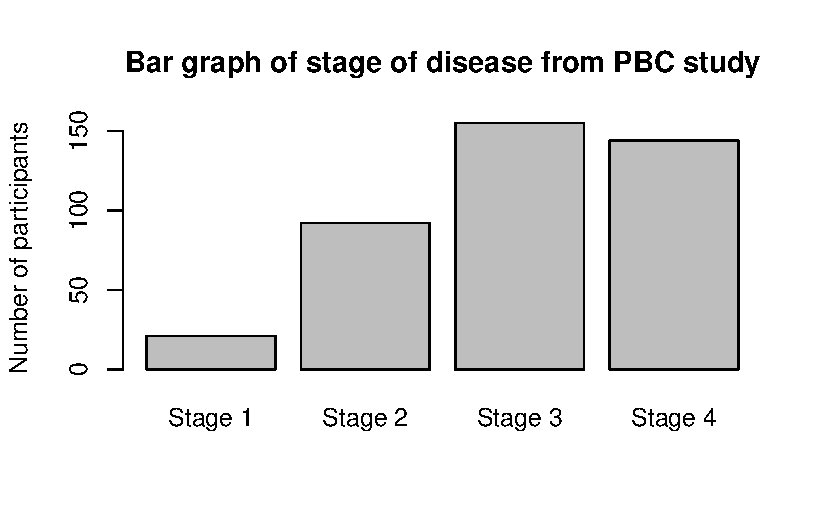
\includegraphics[keepaspectratio]{02-probability_files/figure-pdf/unnamed-chunk-7-1.pdf}}

Note that stage is a categorical variable, that has been defined as a
factor (in Section~\ref{sec-cat-as-factors}). You \textbf{must define
categorical data as factors} to plot them in a bar graph.

\section{Creating bar charts for two categorical
variables}\label{creating-bar-charts-for-two-categorical-variables-1}

\subsection{Option 1: Using the contTables
function}\label{option-1-using-the-conttables-function}

Creating a \textbf{clustered bar chart} as shown in
Figure~\ref{fig-bar-2} can be done easily using the \texttt{contTables}
function in the \texttt{jmv} package. First create a cross-tab from the
variables to be plotted, for example, Stage by Sex:

\begin{Shaded}
\begin{Highlighting}[]
\FunctionTok{contTables}\NormalTok{(}\AttributeTok{data =}\NormalTok{ pbc, }\AttributeTok{rows =}\NormalTok{ sex, }\AttributeTok{cols =}\NormalTok{ stage)}
\end{Highlighting}
\end{Shaded}

\begin{verbatim}

 CONTINGENCY TABLES

 Contingency Tables                                              
 ─────────────────────────────────────────────────────────────── 
   sex       Stage 1    Stage 2    Stage 3    Stage 4    Total   
 ─────────────────────────────────────────────────────────────── 
   Male            3          8         16         17       44   
   Female         18         84        139        127      368   
   Total          21         92        155        144      412   
 ─────────────────────────────────────────────────────────────── 


 χ² Tests                               
 ────────────────────────────────────── 
         Value        df    p           
 ────────────────────────────────────── 
   χ²    0.8779873     3    0.8307365   
   N           412                      
 ────────────────────────────────────── 
\end{verbatim}

Creating a \textbf{clustered bar chart} as shown in
Figure~\ref{fig-bar-2} can be done by requesting a bar chart
(\texttt{barplot=TRUE}), and the x-axis should be constructed from
\texttt{stage} - that is, the \textbf{column} variable:

\begin{Shaded}
\begin{Highlighting}[]
\FunctionTok{contTables}\NormalTok{(pbc, }\AttributeTok{rows =}\NormalTok{ sex, }\AttributeTok{cols =}\NormalTok{ stage, }\AttributeTok{barplot =} \ConstantTok{TRUE}\NormalTok{, }\AttributeTok{xaxis =} \StringTok{"xcols"}\NormalTok{)}
\end{Highlighting}
\end{Shaded}

\begin{verbatim}

 CONTINGENCY TABLES

 Contingency Tables                                              
 ─────────────────────────────────────────────────────────────── 
   sex       Stage 1    Stage 2    Stage 3    Stage 4    Total   
 ─────────────────────────────────────────────────────────────── 
   Male            3          8         16         17       44   
   Female         18         84        139        127      368   
   Total          21         92        155        144      412   
 ─────────────────────────────────────────────────────────────── 


 χ² Tests                               
 ────────────────────────────────────── 
         Value        df    p           
 ────────────────────────────────────── 
   χ²    0.8779873     3    0.8307365   
   N           412                      
 ────────────────────────────────────── 
\end{verbatim}

\pandocbounded{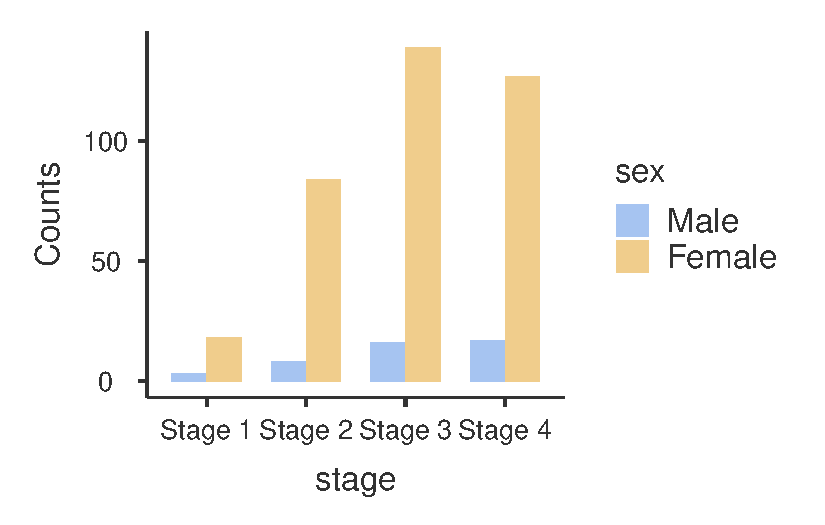
\includegraphics[keepaspectratio]{02-probability_files/figure-pdf/unnamed-chunk-9-1.pdf}}

If you want the x-axis to be constructed from the row variable, you
would use \texttt{xaxis\ =\ "xrows"}.

To create a \textbf{stacked bar chart} (as in Figure~\ref{fig-bar-3}),
specify \texttt{bartype} to be \texttt{stack}:

\begin{Shaded}
\begin{Highlighting}[]
\FunctionTok{contTables}\NormalTok{(}
\NormalTok{  pbc,}
  \AttributeTok{rows =}\NormalTok{ sex,}
  \AttributeTok{cols =}\NormalTok{ stage,}
  \AttributeTok{barplot =} \ConstantTok{TRUE}\NormalTok{,}
  \AttributeTok{xaxis =} \StringTok{"xcols"}\NormalTok{,}
  \AttributeTok{bartype =} \StringTok{"stack"}
\NormalTok{)}
\end{Highlighting}
\end{Shaded}

\begin{verbatim}

 CONTINGENCY TABLES

 Contingency Tables                                              
 ─────────────────────────────────────────────────────────────── 
   sex       Stage 1    Stage 2    Stage 3    Stage 4    Total   
 ─────────────────────────────────────────────────────────────── 
   Male            3          8         16         17       44   
   Female         18         84        139        127      368   
   Total          21         92        155        144      412   
 ─────────────────────────────────────────────────────────────── 


 χ² Tests                               
 ────────────────────────────────────── 
         Value        df    p           
 ────────────────────────────────────── 
   χ²    0.8779873     3    0.8307365   
   N           412                      
 ────────────────────────────────────── 
\end{verbatim}

\pandocbounded{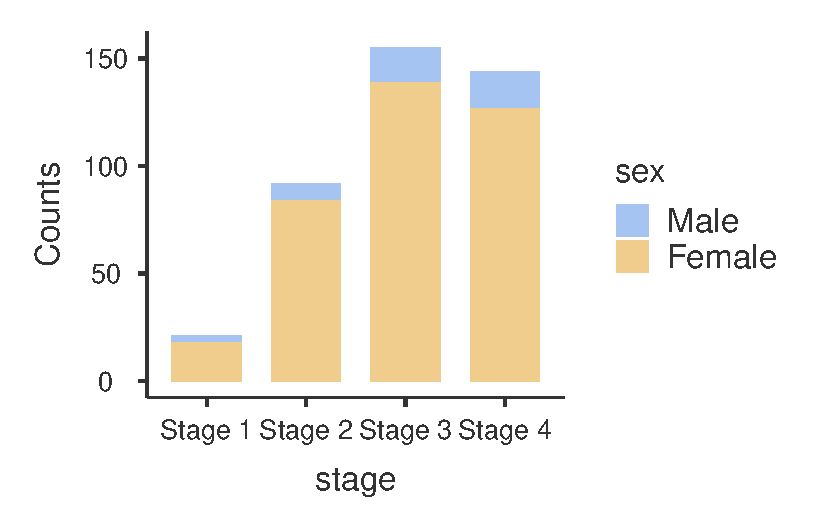
\includegraphics[keepaspectratio]{02-probability_files/figure-pdf/unnamed-chunk-10-1.pdf}}

Finally, to create a \textbf{stacked relative bar chart} (as in
Figure~\ref{fig-bar-4}), specify the y-axis to be a percent
(\texttt{yaxis="ypc"}), and the percentage be calculated from the
columns of the frequency table (\texttt{yaxisPc\ =\ "column\_pc"}):

\begin{Shaded}
\begin{Highlighting}[]
\FunctionTok{contTables}\NormalTok{(}
\NormalTok{  pbc,}
  \AttributeTok{rows =}\NormalTok{ sex,}
  \AttributeTok{cols =}\NormalTok{ stage,}
  \AttributeTok{barplot =} \ConstantTok{TRUE}\NormalTok{,}
  \AttributeTok{bartype =} \StringTok{"stack"}\NormalTok{,}
  \AttributeTok{xaxis =} \StringTok{"xcols"}\NormalTok{,}
  \AttributeTok{yaxis =} \StringTok{"ypc"}\NormalTok{,}
  \AttributeTok{yaxisPc =} \StringTok{"column\_pc"}
\NormalTok{)}
\end{Highlighting}
\end{Shaded}

\begin{verbatim}

 CONTINGENCY TABLES

 Contingency Tables                                              
 ─────────────────────────────────────────────────────────────── 
   sex       Stage 1    Stage 2    Stage 3    Stage 4    Total   
 ─────────────────────────────────────────────────────────────── 
   Male            3          8         16         17       44   
   Female         18         84        139        127      368   
   Total          21         92        155        144      412   
 ─────────────────────────────────────────────────────────────── 


 χ² Tests                               
 ────────────────────────────────────── 
         Value        df    p           
 ────────────────────────────────────── 
   χ²    0.8779873     3    0.8307365   
   N           412                      
 ────────────────────────────────────── 
\end{verbatim}

\pandocbounded{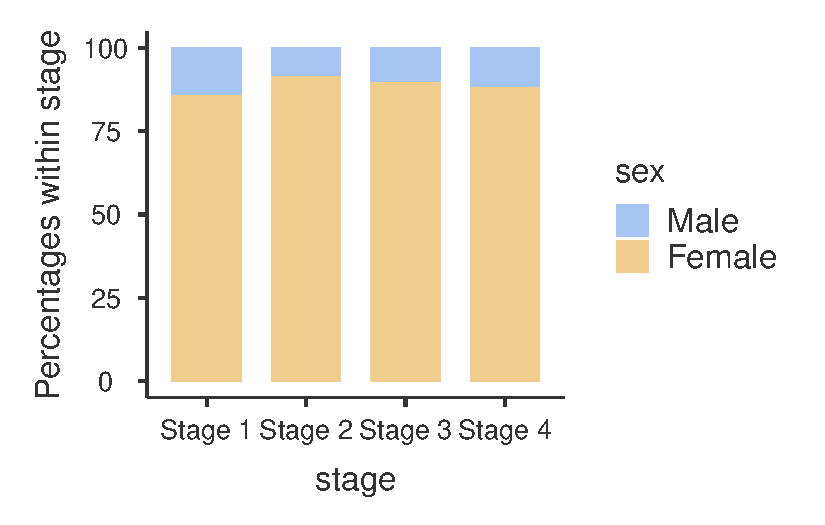
\includegraphics[keepaspectratio]{02-probability_files/figure-pdf/unnamed-chunk-11-1.pdf}}

\subsection{Option 2: Using surveyPlot
function}\label{option-2-using-surveyplot-function}

An alternative way of producing barcharts is via a package called
\texttt{surveymv}. Unfortunately, surveymv is not hosted on the standard
package repository, we need to install the package from github.com. This
is a straight-forward process, which involves installing a package
called \texttt{devtools} that allows packages to be installed from
alternative locations:

\begin{Shaded}
\begin{Highlighting}[]
\FunctionTok{install.packages}\NormalTok{(}\StringTok{"devtools"}\NormalTok{)}
\FunctionTok{library}\NormalTok{(devtools)}
\FunctionTok{install\_github}\NormalTok{(}\StringTok{"raviselker/surveymv"}\NormalTok{)}
\end{Highlighting}
\end{Shaded}

These commands have installed the \texttt{surveymv} package. We load the
packing using the standard \texttt{library()} command:

\begin{Shaded}
\begin{Highlighting}[]
\FunctionTok{library}\NormalTok{(surveymv)}
\end{Highlighting}
\end{Shaded}

\texttt{surveymv} has only one function: \texttt{surveyPlot}, with the
following syntax:

\begin{verbatim}
surveyPlot(
  data = babies,
  vars = "Birth weight",
  group = "Age group",
  type = "stacked",
  freq = "perc")
\end{verbatim}

We specify our data (\texttt{data=}), and the main variable to be
plotted (\texttt{vars=}). If we have a grouping variable, we specify a
\texttt{group=} variable. We define the chart to be either a stacked
(\texttt{type\ =\ "stacked"}) or clustered (\texttt{type\ =\ "grouped"})
bar chart, and specify whether to plot frequencies
(\texttt{freq\ =\ "count"}) or percentages (\texttt{freq\ =\ "perc"}).

To demonstrate, we will recreate Figure~\ref{fig-bar-4}, a figure of the
relative frequencies of sex within stage of disease:

\begin{Shaded}
\begin{Highlighting}[]
\FunctionTok{library}\NormalTok{(surveymv)}

\FunctionTok{surveyPlot}\NormalTok{(}
  \AttributeTok{data =}\NormalTok{ pbc,}
  \AttributeTok{vars =} \StringTok{"sex"}\NormalTok{,}
  \AttributeTok{group =} \StringTok{"stage"}\NormalTok{,}
  \AttributeTok{type =} \StringTok{"stacked"}\NormalTok{,}
  \AttributeTok{freq =} \StringTok{"perc"}
\NormalTok{)}
\end{Highlighting}
\end{Shaded}

\begin{verbatim}

 SURVEY PLOTS
\end{verbatim}

\pandocbounded{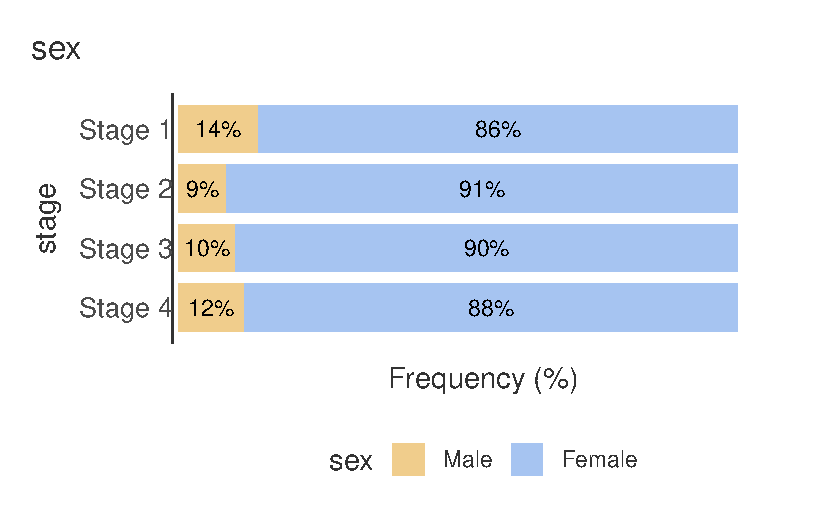
\includegraphics[keepaspectratio]{02-probability_files/figure-pdf/unnamed-chunk-14-1.pdf}}

While this produces a bar chart with horizontal bars, it often performs
better with labelling of the groups than the previous method.

\section{Importing data into R}\label{importing-data-into-r}

We have described previously how to import data that have been saved as
R .rds files. It is quite common to have data saved in other file types,
such as Microsoft Excel, or plain text files. In this section, we will
demonstrate how to import data from other packages into R.

There are two useful packages for importing data into R: \texttt{haven}
(for data that have been saved by jamovi, SAS or SPSS) and
\texttt{readxl} (for data saved by Microsoft Excel). Additionally, the
\texttt{labelled} package is useful in working with data that have been
labelled in jamovi.

\subsection{Importing plain text data into
R}\label{importing-plain-text-data-into-r}

A \texttt{csv} file, or a ``comma separated variables'' file is commonly
used to store data. These files have a very simple structure: they are
plain text files, where data are separated by commas. csv files have the
advantage that, as they are plain text files, they can be opened by a
large number of programs (such as Notepad in Windows, TextEdit in MacOS,
Microsoft Excel - even Microsoft Word). While they can be opened by
Microsoft Excel, they can be opened by many other programs: the csv file
can be thought of as the lingua-franca of data.

In this demonstration, we will use data on the weight of 1000 people
entered in a csv file called \texttt{mod02\_weight\_1000.csv}.

To confirm that the file is readable by any text editor, here are the
first ten lines of the file, opened in Notepad on Microsoft Windows, and
TextEdit on MacOS.

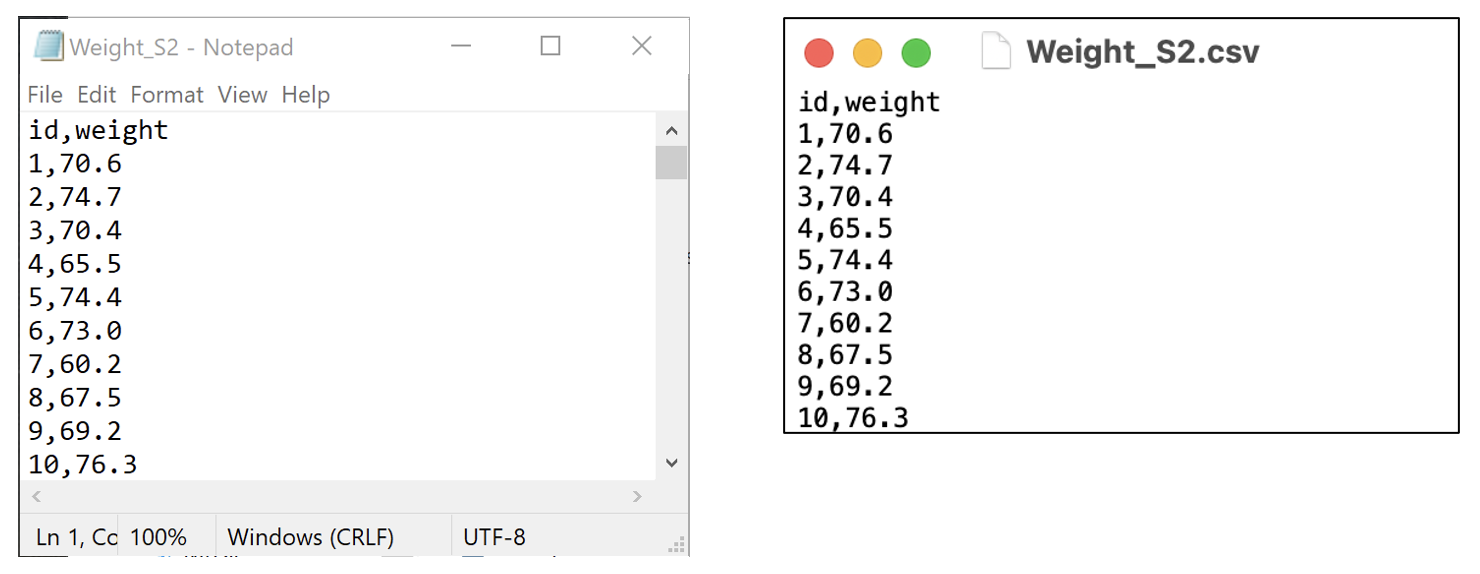
\includegraphics[width=0.66\linewidth,height=\textheight,keepaspectratio]{img/mod02/import-01.png}

We can use the \texttt{read.csv} function:

\begin{Shaded}
\begin{Highlighting}[]
\NormalTok{sample }\OtherTok{\textless{}{-}} \FunctionTok{read.csv}\NormalTok{(}\StringTok{"data/examples/mod02\_weight\_1000.csv"}\NormalTok{)}
\end{Highlighting}
\end{Shaded}

Here, the \texttt{read.csv} function has the default that the first row
of the dataset contains the variable names. If your data do not have
column names, you can use \texttt{header=FALSE} in the function.

Note: there is an alternative function \texttt{read\_csv} which is part
of the \texttt{readr} package (a component of the \texttt{tidyverse}).
Some would argue that the \texttt{read\_csv} function is more
appropriate to use because of an issue known as
\texttt{strings.as.factors}. The \texttt{strings.as.factors} default was
removed in R Version 4.0.0, so it is less important which of the two
functions you use to import a \texttt{.csv} file. More information about
this issue can be found
\href{https://simplystatistics.org/posts/2015-07-24-stringsasfactors-an-unauthorized-biography}{here}
and
\href{https://developer.r-project.org/Blog/public/2020/02/16/stringsasfactors/}{here}.

\section{Recoding data}\label{sec-recoding-data}

One task that is common in statistical computing is to recode variables.
For example, we might want to group some categories of a categorical
variable, or to present a continuous variable in a categorical way.

In this example, we can use the \texttt{pbc} data and recode age into
age groups:

\begin{itemize}
\tightlist
\item
  Less than 30
\item
  30 to less than 50
\item
  50 to less than 70
\item
  70 or older
\end{itemize}

The quickest way to recode a continuous variable into categories is to
use the \texttt{cut} command which takes a continuous variable, and
``cuts'' it into groups based on the specified ``cutpoints''

\begin{Shaded}
\begin{Highlighting}[]
\NormalTok{pbc}\SpecialCharTok{$}\NormalTok{agegroup }\OtherTok{\textless{}{-}} \FunctionTok{cut}\NormalTok{(pbc}\SpecialCharTok{$}\NormalTok{age, }\AttributeTok{breaks =} \FunctionTok{c}\NormalTok{(}\DecValTok{0}\NormalTok{, }\DecValTok{30}\NormalTok{, }\DecValTok{50}\NormalTok{, }\DecValTok{70}\NormalTok{, }\DecValTok{100}\NormalTok{))}
\end{Highlighting}
\end{Shaded}

Notice that some numbers need to be defined for the lowest (age=0) and
highest (age=100) bounds: both a lower and upper limit must be defined
for each group.

If we examine the new \texttt{agegroup} variable:

\begin{Shaded}
\begin{Highlighting}[]
\FunctionTok{summary}\NormalTok{(pbc}\SpecialCharTok{$}\NormalTok{agegroup)}
\end{Highlighting}
\end{Shaded}

\begin{verbatim}
  (0,30]  (30,50]  (50,70] (70,100] 
       3      192      210       13 
\end{verbatim}

we see that each group has been labelled in the form of (a, b{]}. This
notation is equivalent to: greater than a, and less than or equal to b.
The \texttt{cut} function excludes the lower limit, but includes the
upper limit. Our age groups have been defined to include the lower
limit, and exclude the upper limit (for example, greater than or equal
to 30 and less than 50).

We can specify this recoding using the \texttt{right=FALSE} option:

\begin{Shaded}
\begin{Highlighting}[]
\NormalTok{pbc}\SpecialCharTok{$}\NormalTok{agegroup }\OtherTok{\textless{}{-}} \FunctionTok{cut}\NormalTok{(pbc}\SpecialCharTok{$}\NormalTok{age, }\AttributeTok{breaks =} \FunctionTok{c}\NormalTok{(}\DecValTok{0}\NormalTok{, }\DecValTok{30}\NormalTok{, }\DecValTok{50}\NormalTok{, }\DecValTok{70}\NormalTok{, }\DecValTok{100}\NormalTok{), }\AttributeTok{right =} \ConstantTok{FALSE}\NormalTok{)}

\FunctionTok{summary}\NormalTok{(pbc}\SpecialCharTok{$}\NormalTok{agegroup)}
\end{Highlighting}
\end{Shaded}

\begin{verbatim}
  [0,30)  [30,50)  [50,70) [70,100) 
       3      192      210       13 
\end{verbatim}

Finally, we can specify labels for the groups using the \texttt{labels}
option:

\begin{Shaded}
\begin{Highlighting}[]
\NormalTok{pbc}\SpecialCharTok{$}\NormalTok{agegroup }\OtherTok{\textless{}{-}} \FunctionTok{cut}\NormalTok{(}
\NormalTok{  pbc}\SpecialCharTok{$}\NormalTok{age,}
  \AttributeTok{breaks =} \FunctionTok{c}\NormalTok{(}\DecValTok{0}\NormalTok{, }\DecValTok{30}\NormalTok{, }\DecValTok{50}\NormalTok{, }\DecValTok{70}\NormalTok{, }\DecValTok{100}\NormalTok{),}
  \AttributeTok{right =} \ConstantTok{FALSE}\NormalTok{,}
  \AttributeTok{labels =} \FunctionTok{c}\NormalTok{(}
    \StringTok{"Less than 30"}\NormalTok{,}
    \StringTok{"30 to less than 50"}\NormalTok{,}
    \StringTok{"50 to less than 70"}\NormalTok{,}
    \StringTok{"70 or more"}
\NormalTok{  )}
\NormalTok{)}

\FunctionTok{summary}\NormalTok{(pbc}\SpecialCharTok{$}\NormalTok{agegroup)}
\end{Highlighting}
\end{Shaded}

\begin{verbatim}
      Less than 30 30 to less than 50 50 to less than 70         70 or more 
                 3                192                210                 13 
\end{verbatim}

\section{Computing binomial probabilities using R}\label{sec-binom-r}

The Binomial Distribution Applet posted at
\url{https://mabognar.github.io/apps/bin.html}, provides a simple and
intuitive way to compute probabilities from a binomial distribution.
Refer to the jamovi instructions for details.

There are two R functions that we can use to calculate probabilities
based on the binomial distribution: \texttt{dbinom} and \texttt{pbinom}:

\begin{itemize}
\tightlist
\item
  \texttt{dbinom(x,\ size,\ prob)} gives the probability of obtaining
  \texttt{x} successes from \texttt{size} trials when the probability of
  a success on one trial is \texttt{prob};
\item
  \texttt{pbinom(q,\ size,\ prob)} gives the probability of obtaining
  \texttt{q} \textbf{or fewer} successes from \texttt{size} trials when
  the probability of a success on one trial is \texttt{prob};
\item
  \texttt{pbinom(q,\ size,\ prob,\ lower.tail=FALSE)} gives the
  probability of obtaining \textbf{more than} \texttt{q}successes from
  \texttt{size} trials when the probability of a success on one trial is
  \texttt{prob}.
\end{itemize}

To do the computation for part (a) in Worked Example 2.1, we will use
the \texttt{dbinom} function with:

\begin{itemize}
\tightlist
\item
  \emph{x} is the number of successes, here, the number of smokers
  (i.e.~k=3);
\item
  \emph{size} is the number of trials (i.e.~n=6);
\item
  and \emph{prob} is probability of drawing a smoker from the
  population, which is 19.8\% (i.e.~p=0.198).
\end{itemize}

Replace each of these with the appropriate number into the formula:

\begin{Shaded}
\begin{Highlighting}[]
\FunctionTok{dbinom}\NormalTok{(}\AttributeTok{x =} \DecValTok{3}\NormalTok{, }\AttributeTok{size =} \DecValTok{6}\NormalTok{, }\AttributeTok{prob =} \FloatTok{0.198}\NormalTok{)}
\end{Highlighting}
\end{Shaded}

\begin{verbatim}
[1] 0.08008454
\end{verbatim}

To calculate the upper tail of probability in part (b), we use the
\texttt{pbinom(lower.tail=FALSE)} function. Note that the
\texttt{pbinom(lower.tail=FALSE)} function \textbf{does not include
\texttt{q}}, so to obtain 4 or more successes, we need to enter
\texttt{q=3}:

\begin{Shaded}
\begin{Highlighting}[]
\FunctionTok{pbinom}\NormalTok{(}\AttributeTok{q =} \DecValTok{3}\NormalTok{, }\AttributeTok{size =} \DecValTok{6}\NormalTok{, }\AttributeTok{prob =} \FloatTok{0.198}\NormalTok{, }\AttributeTok{lower.tail =} \ConstantTok{FALSE}\NormalTok{)}
\end{Highlighting}
\end{Shaded}

\begin{verbatim}
[1] 0.01635325
\end{verbatim}

For the lower tail for part (c), we use the \texttt{pbinom} function:

\begin{Shaded}
\begin{Highlighting}[]
\FunctionTok{pbinom}\NormalTok{(}\AttributeTok{q =} \DecValTok{2}\NormalTok{, }\AttributeTok{size =} \DecValTok{6}\NormalTok{, }\AttributeTok{prob =} \FloatTok{0.198}\NormalTok{)}
\end{Highlighting}
\end{Shaded}

\begin{verbatim}
[1] 0.9035622
\end{verbatim}

\begin{tcolorbox}[enhanced jigsaw, arc=.35mm, bottomrule=.15mm, bottomtitle=1mm, breakable, colback=white, colbacktitle=quarto-callout-note-color!10!white, colframe=quarto-callout-note-color-frame, coltitle=black, left=2mm, leftrule=.75mm, opacityback=0, opacitybacktitle=0.6, rightrule=.15mm, title=\textcolor{quarto-callout-note-color}{\faInfo}\hspace{0.5em}{Note}, titlerule=0mm, toprule=.15mm, toptitle=1mm]

In this section, we introduce \texttt{ggplot2} which is a very flexible
method of plotting data in R. The use of \texttt{ggplot2} is
\textbf{completely optional}. It is perfectly fine to produce graphs
using the simpler methods, as long as they are formatted appropriately.

\end{tcolorbox}

\section{\texorpdfstring{Introducing
\texttt{ggplot2}}{Introducing ggplot2}}\label{introducing-ggplot2}

Plots produced by \texttt{plot(dens())} and \texttt{boxplot()} are often
called \texttt{base} graphics: no special packages have been needed to
produce these plots. In this section, we will introduce the
\texttt{ggplot2} \footnote{Note that the package is called
  \texttt{ggplot2} as it is a complete overhaul of the package called
  \texttt{ggplot}. The main function used in the \texttt{ggplot2}
  package is \texttt{ggplot()}. This can be confusing, but you will get
  used to this in time.} package, which defines plots using a
\textbf{grammar of graphics}. This can seem like a complex way of
constructing a plot, but the framework allows for very complex plots to
be constructed in a relatively consistent way.

The grammar of graphics defines a number of elements of a plot; the key
elements that we will use in this course are:

\begin{itemize}
\tightlist
\item
  data: we need to specify the data we are plotting. The data must be
  stored as a dataframe, where variables are organised in columns, and
  observations are in rows
\item
  mapping: the \emph{aesthetic mapping} describes how your data map to
  visual properties of the plot. For example, we might want to define
  the x-axis by the \texttt{age} variable and the colour of points by
  \texttt{sex}. We can define our mapping using the command
  \texttt{mapping\ =\ aes()}, and entering the specific aesthetic
  components within the \texttt{aes()} component.
\item
  geometries: we can think of \emph{geometries} as defining the actual
  ``ink'' of the plot, modified by the \emph{aesthetics} defined by the
  mapping. For example:

  \begin{itemize}
  \tightlist
  \item
    \texttt{geom\_bar()} will plot a bar-chart;
  \item
    \texttt{geom\_boxplot()} will plot a boxplot;
  \item
    \texttt{geom\_histogram()} will plot a histogram.
  \end{itemize}
\item
  theme: the \emph{theme} defines the overall look of the plot. Every
  part of the plot that is not specified by data can be adjusted by
  changing the theme. For example, fonts, axis ticks, legend position
  and background colours can all be changed by using a theme. Some
  useful themes are:

  \begin{itemize}
  \tightlist
  \item
    \texttt{theme\_bw()}: a black-and-white theme
  \item
    \texttt{theme\_minimal()}: a clean them with no background
    annotations
  \item
    \texttt{theme\_classic()}: a theme that removes grid-lines and
    backgrounds, leaving only axis lines.
  \end{itemize}
\end{itemize}

These elements can be combined in a single \texttt{ggplot} command by
using a \texttt{+} symbol, usually with each element provided on a new
line.

\subsection{\texorpdfstring{Using \texttt{ggplot2} to construct a bar
chart}{Using ggplot2 to construct a bar chart}}\label{using-ggplot2-to-construct-a-bar-chart}

As a demonstration, we will produce the simplest bar chart possible: a
bar chart of \texttt{sex}.

First, we will load the \texttt{ggplot2} library, and call the
\texttt{ggplot} function with no function arguments.

\begin{Shaded}
\begin{Highlighting}[]
\FunctionTok{library}\NormalTok{(ggplot2)}

\FunctionTok{ggplot}\NormalTok{()}
\end{Highlighting}
\end{Shaded}

\pandocbounded{
\includegraphics[keepaspectratio]{02-probability_files/figure-pdf/unnamed-chunk-24-1.pdf}}

In this example, all \texttt{ggplot} has done is to create a blank
canvas. Let's start filling the canvas in by specifying our dataset, and
defining sex as our x-axis:

\begin{Shaded}
\begin{Highlighting}[]
\FunctionTok{ggplot}\NormalTok{(}\AttributeTok{data =}\NormalTok{ pbc, }\AttributeTok{mapping =} \FunctionTok{aes}\NormalTok{(}\AttributeTok{x =}\NormalTok{ sex))}
\end{Highlighting}
\end{Shaded}

\pandocbounded{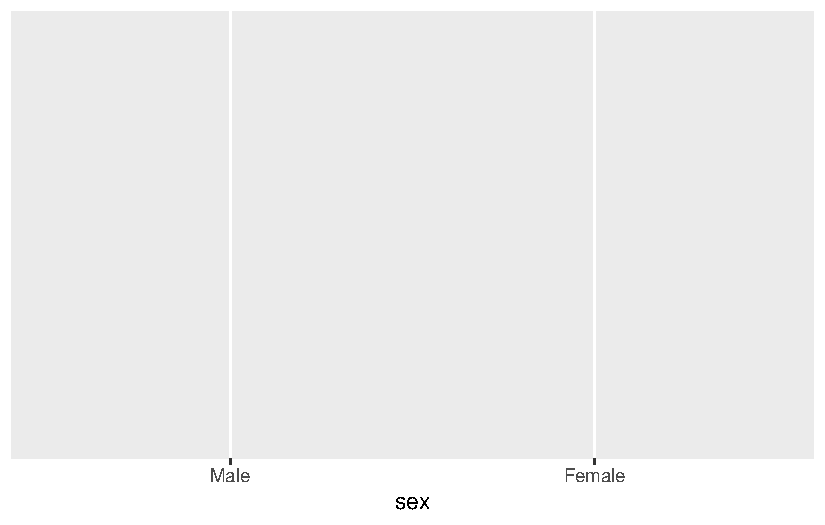
\includegraphics[keepaspectratio]{02-probability_files/figure-pdf/unnamed-chunk-25-1.pdf}}

Our blank canvas has been altered: we now have an x-axis, defined by
\texttt{sex}, with values of \texttt{Male} and \texttt{Female}.

To add ``ink'' to our canvas, we now need to add a \emph{geometry}. For
a bar chart, we use \texttt{geom\_bar()} as follows:

\begin{Shaded}
\begin{Highlighting}[]
\FunctionTok{ggplot}\NormalTok{(}\AttributeTok{data =}\NormalTok{ pbc, }\AttributeTok{mapping =} \FunctionTok{aes}\NormalTok{(}\AttributeTok{x =}\NormalTok{ sex)) }\SpecialCharTok{+}
  \FunctionTok{geom\_bar}\NormalTok{()}
\end{Highlighting}
\end{Shaded}

\pandocbounded{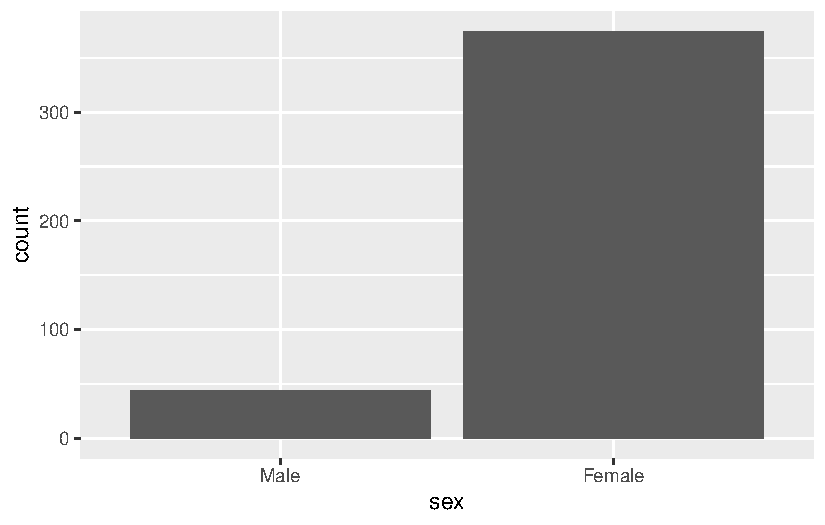
\includegraphics[keepaspectratio]{02-probability_files/figure-pdf/unnamed-chunk-26-1.pdf}}

We can change the look of the figure by choosing a different
\emph{theme}: let's use \texttt{theme\_classic()} here.

\begin{Shaded}
\begin{Highlighting}[]
\FunctionTok{ggplot}\NormalTok{(}\AttributeTok{data =}\NormalTok{ pbc, }\AttributeTok{mapping =} \FunctionTok{aes}\NormalTok{(}\AttributeTok{x =}\NormalTok{ sex)) }\SpecialCharTok{+}
  \FunctionTok{geom\_bar}\NormalTok{() }\SpecialCharTok{+}
  \FunctionTok{theme\_classic}\NormalTok{()}
\end{Highlighting}
\end{Shaded}

\pandocbounded{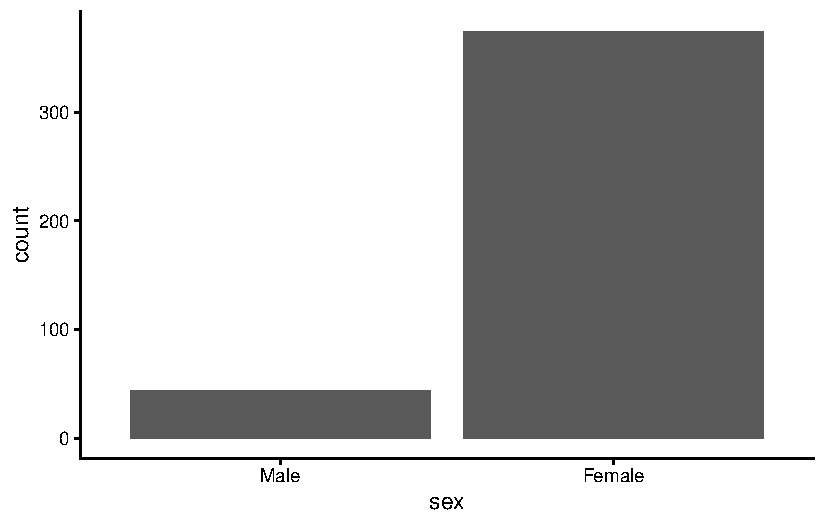
\includegraphics[keepaspectratio]{02-probability_files/figure-pdf/unnamed-chunk-27-1.pdf}}

The final changes we can make are to define the axis labels using
\texttt{labs()}:

\begin{Shaded}
\begin{Highlighting}[]
\FunctionTok{ggplot}\NormalTok{(}\AttributeTok{data =}\NormalTok{ pbc, }\AttributeTok{mapping =} \FunctionTok{aes}\NormalTok{(}\AttributeTok{x =}\NormalTok{ sex)) }\SpecialCharTok{+}
  \FunctionTok{geom\_bar}\NormalTok{() }\SpecialCharTok{+}
  \FunctionTok{theme\_classic}\NormalTok{() }\SpecialCharTok{+}
  \FunctionTok{labs}\NormalTok{(}\AttributeTok{x =} \StringTok{"Participant sex"}\NormalTok{, }\AttributeTok{y =} \StringTok{"Frequency"}\NormalTok{)}
\end{Highlighting}
\end{Shaded}

\pandocbounded{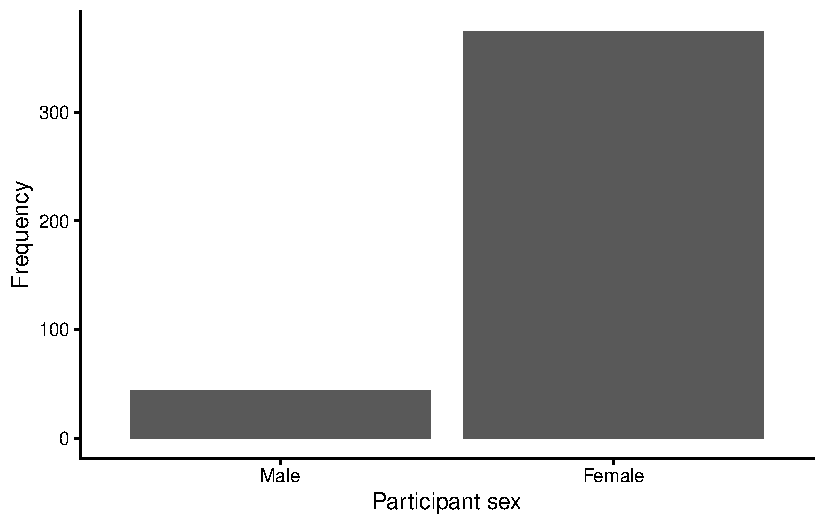
\includegraphics[keepaspectratio]{02-probability_files/figure-pdf/unnamed-chunk-28-1.pdf}}

Finally, we can change the colour of the bars by specifying a
\texttt{fill} colour within the \texttt{geom\_bar()} command. We can
choose one of over 600 (!) colours by name \footnote{A list of available
  colours that can be used in \texttt{ggplot} can be found by entering
  the command \texttt{grDevices::colours()} in R, or by searching the
  web for \texttt{R\ colour\ names}.}.

\begin{Shaded}
\begin{Highlighting}[]
\FunctionTok{ggplot}\NormalTok{(}\AttributeTok{data =}\NormalTok{ pbc, }\AttributeTok{mapping =} \FunctionTok{aes}\NormalTok{(}\AttributeTok{x =}\NormalTok{ sex)) }\SpecialCharTok{+}
  \FunctionTok{geom\_bar}\NormalTok{(}\AttributeTok{fill =} \StringTok{"steelblue"}\NormalTok{) }\SpecialCharTok{+}
  \FunctionTok{theme\_classic}\NormalTok{() }\SpecialCharTok{+}
  \FunctionTok{labs}\NormalTok{(}\AttributeTok{x =} \StringTok{"Participant sex"}\NormalTok{, }\AttributeTok{y =} \StringTok{"Frequency"}\NormalTok{)}
\end{Highlighting}
\end{Shaded}

\pandocbounded{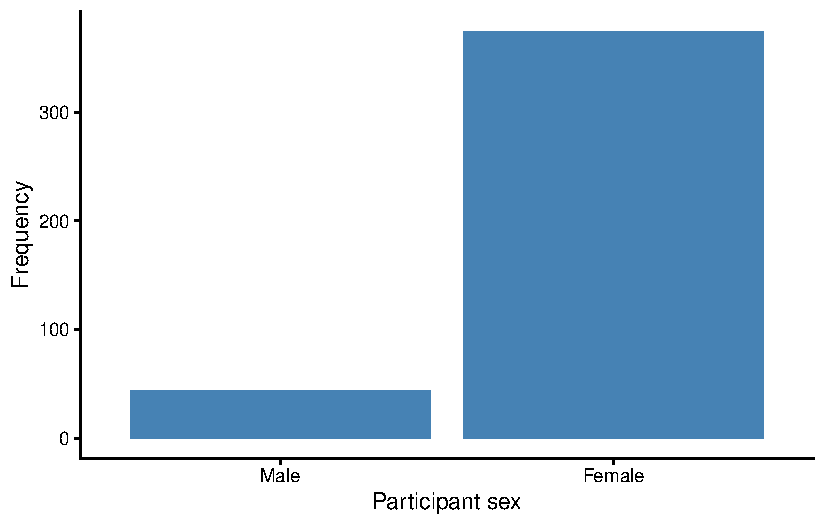
\includegraphics[keepaspectratio]{02-probability_files/figure-pdf/unnamed-chunk-29-1.pdf}}

Let's adapt this code to produce a bar chart for stage of disease:

\begin{Shaded}
\begin{Highlighting}[]
\FunctionTok{ggplot}\NormalTok{(}\AttributeTok{data =}\NormalTok{ pbc, }\AttributeTok{mapping =} \FunctionTok{aes}\NormalTok{(}\AttributeTok{x =}\NormalTok{ stage)) }\SpecialCharTok{+}
  \FunctionTok{geom\_bar}\NormalTok{(}\AttributeTok{fill =} \StringTok{"steelblue"}\NormalTok{) }\SpecialCharTok{+}
  \FunctionTok{theme\_classic}\NormalTok{() }\SpecialCharTok{+}
  \FunctionTok{labs}\NormalTok{(}\AttributeTok{x =} \StringTok{"Stage of disease"}\NormalTok{, }\AttributeTok{y =} \StringTok{"Frequency"}\NormalTok{)}
\end{Highlighting}
\end{Shaded}

\pandocbounded{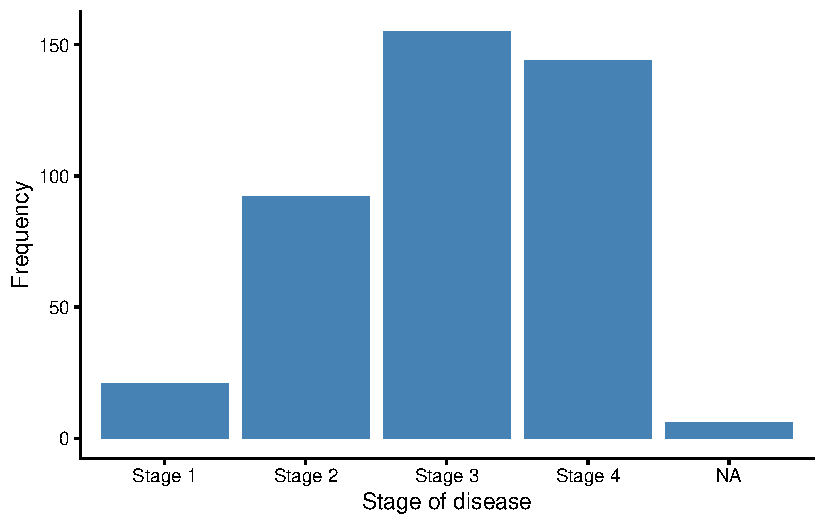
\includegraphics[keepaspectratio]{02-probability_files/figure-pdf/unnamed-chunk-30-1.pdf}}

Note that \texttt{ggplot} has included a separate bar for the missing
values (i.e.~the \texttt{NA} values). We can instruct R to ignore the
missing values in the \texttt{ggplot} function by specifying the data to
be a \texttt{subset} of \texttt{pbc}. The command:
\texttt{subset(pbc,\ is.na(stage)\ ==\ FALSE)} essentially creates a
temporary subset of the \texttt{pbc} dataset where \texttt{stage} is not
missing. Putting it all together:

\begin{Shaded}
\begin{Highlighting}[]
\FunctionTok{ggplot}\NormalTok{(}\AttributeTok{data =} \FunctionTok{subset}\NormalTok{(pbc, }\FunctionTok{is.na}\NormalTok{(stage) }\SpecialCharTok{==} \ConstantTok{FALSE}\NormalTok{), }\AttributeTok{mapping =} \FunctionTok{aes}\NormalTok{(}\AttributeTok{x =}\NormalTok{ stage)) }\SpecialCharTok{+}
  \FunctionTok{geom\_bar}\NormalTok{(}\AttributeTok{fill =} \StringTok{"steelblue"}\NormalTok{) }\SpecialCharTok{+}
  \FunctionTok{theme\_classic}\NormalTok{() }\SpecialCharTok{+}
  \FunctionTok{labs}\NormalTok{(}\AttributeTok{x =} \StringTok{"Stage of disease"}\NormalTok{, }\AttributeTok{y =} \StringTok{"Frequency"}\NormalTok{)}
\end{Highlighting}
\end{Shaded}

\pandocbounded{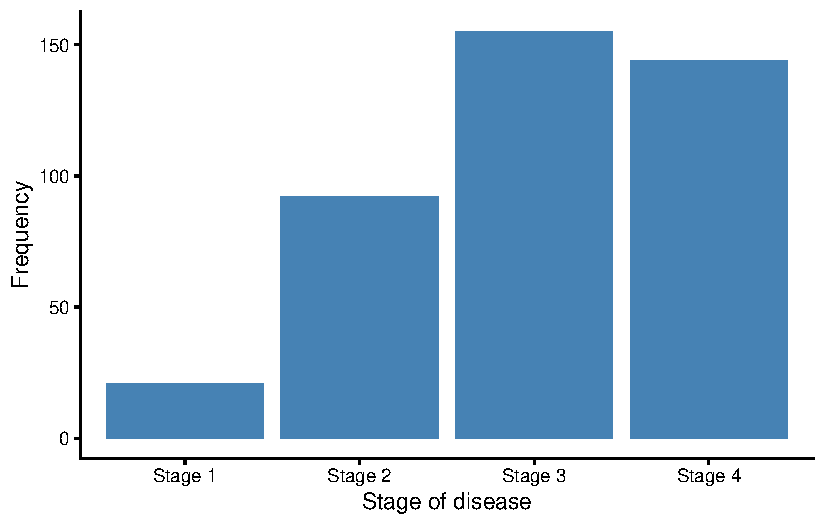
\includegraphics[keepaspectratio]{02-probability_files/figure-pdf/unnamed-chunk-31-1.pdf}}

\section{\texorpdfstring{Introducing the ``pipe''
\texttt{\textbar{}\textgreater{}}}{Introducing the ``pipe'' \textbar\textgreater{}}}\label{introducing-the-pipe}

Consider the previous example, which essentially combines two functions:
\texttt{ggplot()} and \texttt{subset()} by using:
\texttt{ggplot(subset())} - in other words, \texttt{subset()} has been
nested within \texttt{ggplot()}. When R comes across nested functions,
it will happily run the inner-most function first, then applies the
outer function to the result of the inner function.

While this code is understandable by R, one could argue this code is
difficult to understand for a person. A more interpretable version of
this code for a person would be:

\begin{itemize}
\tightlist
\item
  first run the \texttt{subset()} function, \textbf{and then}
\item
  run the \texttt{ggplot()} function.
\end{itemize}

This can be rewritten using the \texttt{\textbar{}\textgreater{}}
symbol:

\begin{verbatim}
subset() |> 
  ggplot()
\end{verbatim}

This syntax would ``pipe'' the results of the first function into the
second function, and produces code that is much easier for a person to
read. So our previous bar chart of stage of disease can be rewritten as:

\begin{Shaded}
\begin{Highlighting}[]
\FunctionTok{subset}\NormalTok{(pbc, }\FunctionTok{is.na}\NormalTok{(stage) }\SpecialCharTok{==} \ConstantTok{FALSE}\NormalTok{) }\SpecialCharTok{|\textgreater{}}
  \FunctionTok{ggplot}\NormalTok{(}\AttributeTok{mapping =} \FunctionTok{aes}\NormalTok{(}\AttributeTok{x =}\NormalTok{ stage)) }\SpecialCharTok{+}
  \FunctionTok{geom\_bar}\NormalTok{(}\AttributeTok{fill =} \StringTok{"steelblue"}\NormalTok{) }\SpecialCharTok{+}
  \FunctionTok{theme\_classic}\NormalTok{() }\SpecialCharTok{+}
  \FunctionTok{labs}\NormalTok{(}\AttributeTok{x =} \StringTok{"Stage of disease"}\NormalTok{, }\AttributeTok{y =} \StringTok{"Frequency"}\NormalTok{)}
\end{Highlighting}
\end{Shaded}

\pandocbounded{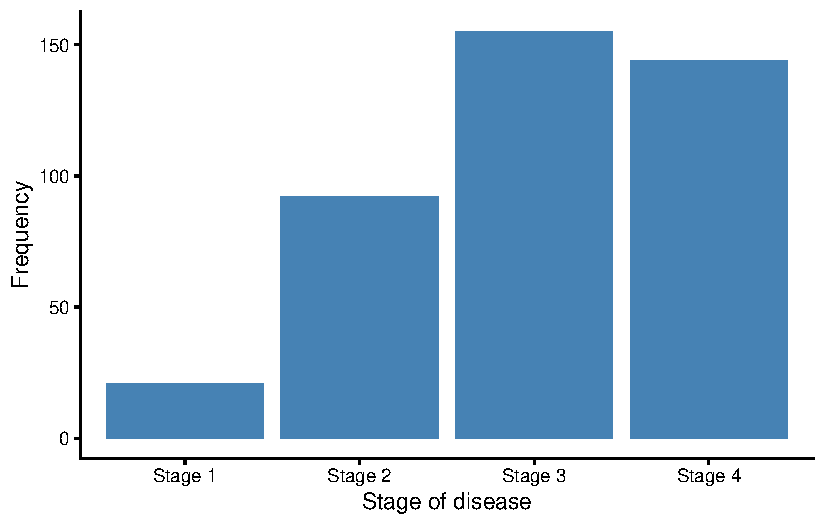
\includegraphics[keepaspectratio]{02-probability_files/figure-pdf/unnamed-chunk-32-1.pdf}}

Notice that when we pipe a dataset from the \texttt{subset()} function,
we no longer need to specify the name of the dataset in
\texttt{ggplot()}: the dataset is inferred from the action of the
\texttt{subset()} function.

\begin{tcolorbox}[enhanced jigsaw, arc=.35mm, bottomrule=.15mm, bottomtitle=1mm, breakable, colback=white, colbacktitle=quarto-callout-note-color!10!white, colframe=quarto-callout-note-color-frame, coltitle=black, left=2mm, leftrule=.75mm, opacityback=0, opacitybacktitle=0.6, rightrule=.15mm, title=\textcolor{quarto-callout-note-color}{\faInfo}\hspace{0.5em}{Note}, titlerule=0mm, toprule=.15mm, toptitle=1mm]

\begin{itemize}
\item
  The \texttt{\textbar{}\textgreater{}} pipe was introduced in R version
  4.1.0, May 2021, and for this author (TD), has drastically improved
  the code that I write (and read!). When reading code that I, or
  others, have written using the pipe, I replace
  \texttt{\textbar{}\textgreater{}} by the words \textbf{and then}. So
  the previous code would be read: subset the data \textbf{and then}
  plot the data.
\item
  You may also see \texttt{\%\textgreater{}\%} referred to as a pipe.
  This version of the pipe was introduced in the early 2010s, most
  notably in the \texttt{magrittr} package. While there are subtle
  differences between \texttt{\textbar{}\textgreater{}} and
  \texttt{\%\textgreater{}\%}, the \texttt{\textbar{}\textgreater{}} is
  the easier to use for this course, as it does not require loading any
  additional packages. More in-depth history can be found at
  \href{http://adolfoalvarez.cl/blog/2021-09-16-plumbers-chains-and-famous-painters-the-history-of-the-pipe-operator-in-r/}{this
  blog post}.
\end{itemize}

\end{tcolorbox}

\subsection{\texorpdfstring{Using \texttt{ggplot2} to construct bar
charts for two
variables}{Using ggplot2 to construct bar charts for two variables}}\label{using-ggplot2-to-construct-bar-charts-for-two-variables}

In Section~\ref{sec-two-catvar-graph}, we saw that clustered or stacked
bar charts can be used to summarise two categorical variables. Remember
that the \emph{aesthetic mapping} can be used to describe how our data
map to visual elements of our plot. So we can map \texttt{sex} to the
\texttt{fill} attribute to summarise Stage of Disease by sex. By
default, \texttt{ggplot} will produce a stacked bar chart, but we can
request a clustered bar chart by specifying \texttt{position="dodge"} in
the \texttt{geom\_bar()} statement:

\begin{Shaded}
\begin{Highlighting}[]
\FunctionTok{subset}\NormalTok{(pbc, }\FunctionTok{is.na}\NormalTok{(stage) }\SpecialCharTok{==} \ConstantTok{FALSE}\NormalTok{) }\SpecialCharTok{|\textgreater{}}
  \FunctionTok{ggplot}\NormalTok{(}\AttributeTok{mapping =} \FunctionTok{aes}\NormalTok{(}\AttributeTok{x =}\NormalTok{ stage, }\AttributeTok{fill =}\NormalTok{ sex)) }\SpecialCharTok{+}
  \FunctionTok{geom\_bar}\NormalTok{(}\AttributeTok{position =} \StringTok{"dodge"}\NormalTok{) }\SpecialCharTok{+}
  \FunctionTok{theme\_classic}\NormalTok{() }\SpecialCharTok{+}
  \FunctionTok{labs}\NormalTok{(}\AttributeTok{x =} \StringTok{"Stage of disease"}\NormalTok{, }\AttributeTok{y =} \StringTok{"Frequency"}\NormalTok{)}
\end{Highlighting}
\end{Shaded}

\pandocbounded{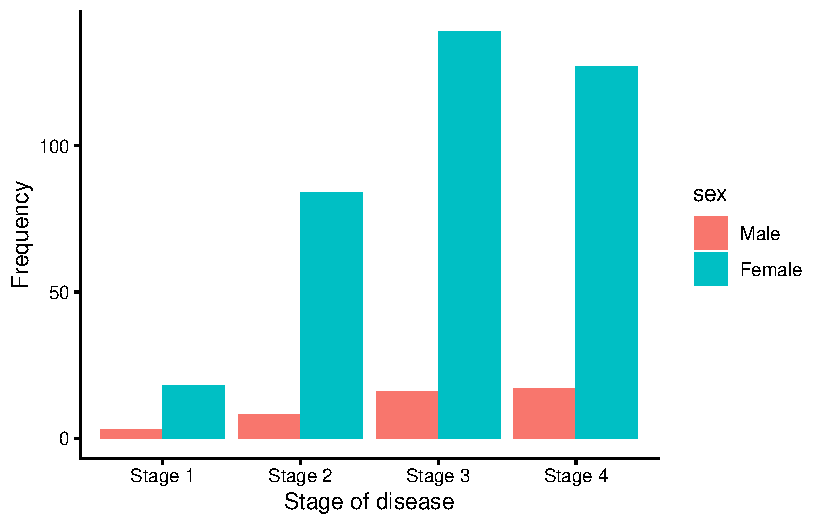
\includegraphics[keepaspectratio]{02-probability_files/figure-pdf/unnamed-chunk-33-1.pdf}}

Notice that the legend title uses the name of the \texttt{fill}
variable, in this case \texttt{sex} with a lower-case s. We can specify
an alternative legend title in the \texttt{labs()} statement:

\begin{Shaded}
\begin{Highlighting}[]
\FunctionTok{subset}\NormalTok{(pbc, }\FunctionTok{is.na}\NormalTok{(stage) }\SpecialCharTok{==} \ConstantTok{FALSE}\NormalTok{) }\SpecialCharTok{|\textgreater{}}
  \FunctionTok{ggplot}\NormalTok{(}\AttributeTok{mapping =} \FunctionTok{aes}\NormalTok{(}\AttributeTok{x =}\NormalTok{ stage, }\AttributeTok{fill =}\NormalTok{ sex)) }\SpecialCharTok{+}
  \FunctionTok{geom\_bar}\NormalTok{(}\AttributeTok{position =} \StringTok{"dodge"}\NormalTok{) }\SpecialCharTok{+}
  \FunctionTok{theme\_classic}\NormalTok{() }\SpecialCharTok{+}
  \FunctionTok{labs}\NormalTok{(}\AttributeTok{x =} \StringTok{"Stage of disease"}\NormalTok{, }\AttributeTok{y =} \StringTok{"Frequency"}\NormalTok{, }\AttributeTok{fill =} \StringTok{"Sex"}\NormalTok{)}
\end{Highlighting}
\end{Shaded}

\pandocbounded{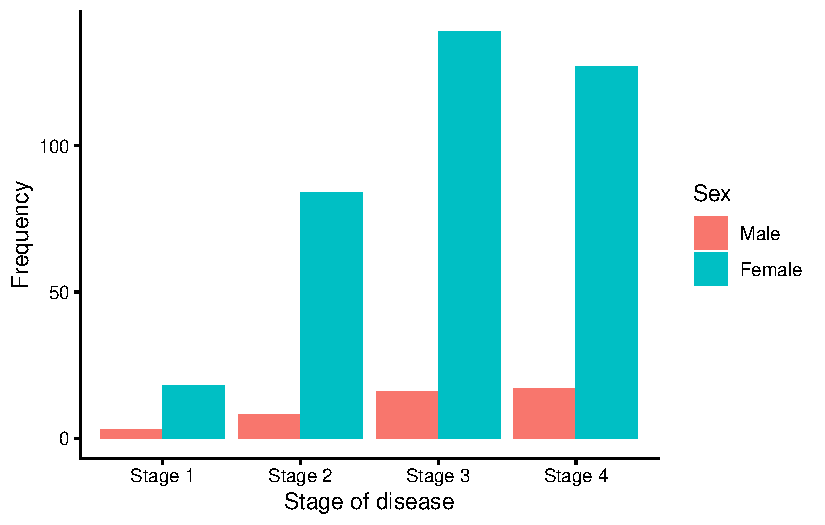
\includegraphics[keepaspectratio]{02-probability_files/figure-pdf/unnamed-chunk-34-1.pdf}}

A stacked bar chart can be constructed by removing the
\texttt{position\ =\ dodge()} statement:

\begin{Shaded}
\begin{Highlighting}[]
\FunctionTok{subset}\NormalTok{(pbc, }\FunctionTok{is.na}\NormalTok{(stage) }\SpecialCharTok{==} \ConstantTok{FALSE}\NormalTok{) }\SpecialCharTok{|\textgreater{}}
  \FunctionTok{ggplot}\NormalTok{(}\AttributeTok{mapping =} \FunctionTok{aes}\NormalTok{(}\AttributeTok{x =}\NormalTok{ stage, }\AttributeTok{fill =}\NormalTok{ sex)) }\SpecialCharTok{+}
  \FunctionTok{geom\_bar}\NormalTok{() }\SpecialCharTok{+}
  \FunctionTok{theme\_classic}\NormalTok{() }\SpecialCharTok{+}
  \FunctionTok{labs}\NormalTok{(}\AttributeTok{x =} \StringTok{"Stage of disease"}\NormalTok{, }\AttributeTok{y =} \StringTok{"Frequency"}\NormalTok{, }\AttributeTok{fill =} \StringTok{"Sex"}\NormalTok{)}
\end{Highlighting}
\end{Shaded}

\pandocbounded{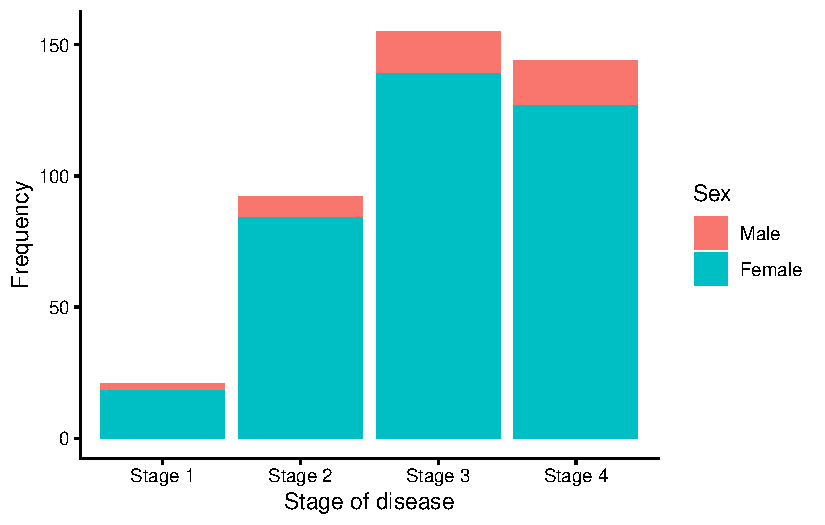
\includegraphics[keepaspectratio]{02-probability_files/figure-pdf/unnamed-chunk-35-1.pdf}}

Finally, we can construct a stacked relative bar chart by specifying
\texttt{position\ =\ "fill"} in the \texttt{geom\_bar()} definition:

\begin{Shaded}
\begin{Highlighting}[]
\FunctionTok{subset}\NormalTok{(pbc, }\FunctionTok{is.na}\NormalTok{(stage) }\SpecialCharTok{==} \ConstantTok{FALSE}\NormalTok{) }\SpecialCharTok{|\textgreater{}}
  \FunctionTok{ggplot}\NormalTok{(}\AttributeTok{mapping =} \FunctionTok{aes}\NormalTok{(}\AttributeTok{x =}\NormalTok{ stage, }\AttributeTok{fill =}\NormalTok{ sex)) }\SpecialCharTok{+}
  \FunctionTok{geom\_bar}\NormalTok{(}\AttributeTok{position =} \StringTok{"fill"}\NormalTok{) }\SpecialCharTok{+}
  \FunctionTok{theme\_classic}\NormalTok{() }\SpecialCharTok{+}
  \FunctionTok{labs}\NormalTok{(}\AttributeTok{x =} \StringTok{"Stage of disease"}\NormalTok{, }\AttributeTok{y =} \StringTok{"Proportion"}\NormalTok{, }\AttributeTok{fill =} \StringTok{"Sex"}\NormalTok{)}
\end{Highlighting}
\end{Shaded}

\pandocbounded{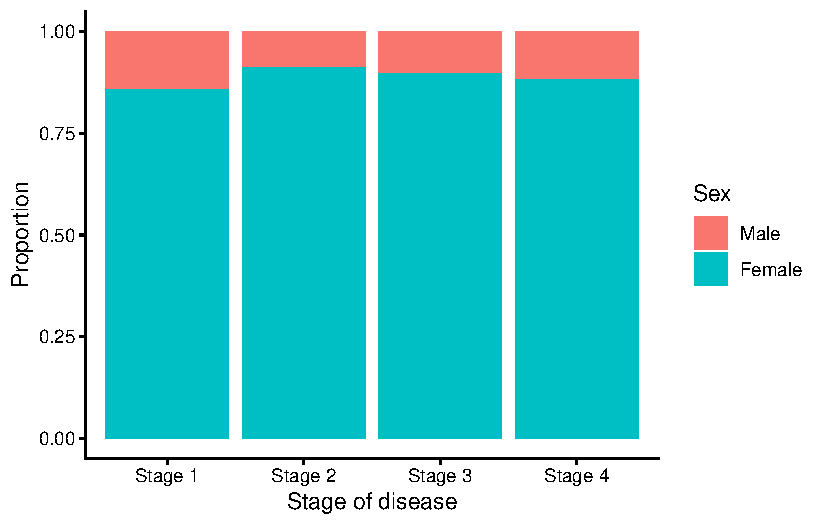
\includegraphics[keepaspectratio]{02-probability_files/figure-pdf/unnamed-chunk-36-1.pdf}}

\section{Producing a density plot using
ggplot}\label{producing-a-density-plot-using-ggplot}

We can produce a density plot by specifying the variable of interest as
the \texttt{x} variable, and requesting a \texttt{geom\_density()}:

\begin{Shaded}
\begin{Highlighting}[]
\FunctionTok{ggplot}\NormalTok{(}\AttributeTok{data =}\NormalTok{ pbc, }\FunctionTok{aes}\NormalTok{(}\AttributeTok{x =}\NormalTok{ age)) }\SpecialCharTok{+}
  \FunctionTok{geom\_density}\NormalTok{() }\SpecialCharTok{+}
  \FunctionTok{theme\_classic}\NormalTok{() }\SpecialCharTok{+}
  \FunctionTok{labs}\NormalTok{(}\AttributeTok{x =} \StringTok{"Age (years)"}\NormalTok{, }\AttributeTok{y =} \StringTok{"Density"}\NormalTok{)}
\end{Highlighting}
\end{Shaded}

\pandocbounded{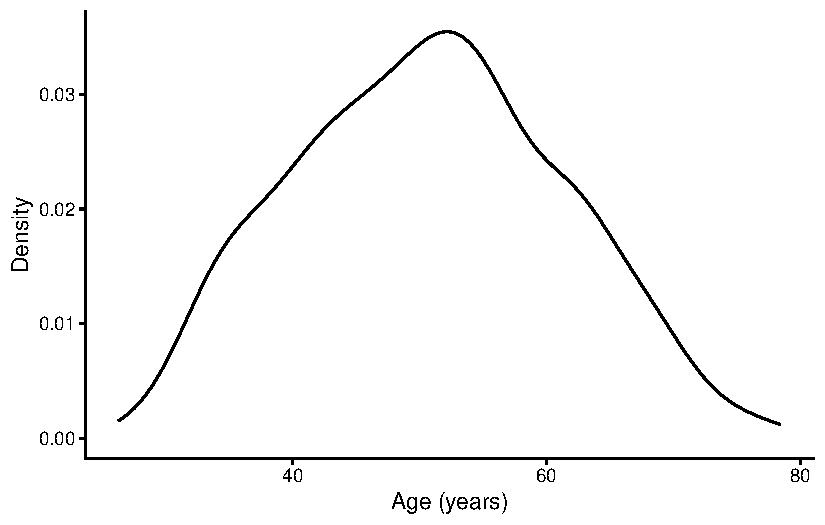
\includegraphics[keepaspectratio]{02-probability_files/figure-pdf/unnamed-chunk-37-1.pdf}}

\section{Producing a boxplot using
ggplot}\label{producing-a-boxplot-using-ggplot}

A boxplot is constructed with a single \texttt{y} variable, and
\texttt{geom\_boxplot()}:

\begin{Shaded}
\begin{Highlighting}[]
\FunctionTok{ggplot}\NormalTok{(}\AttributeTok{data =}\NormalTok{ pbc, }\FunctionTok{aes}\NormalTok{(}\AttributeTok{y =}\NormalTok{ age)) }\SpecialCharTok{+}
  \FunctionTok{geom\_boxplot}\NormalTok{() }\SpecialCharTok{+}
  \FunctionTok{theme\_classic}\NormalTok{() }\SpecialCharTok{+}
  \FunctionTok{labs}\NormalTok{(}\AttributeTok{y =} \StringTok{"Age (years)"}\NormalTok{)}
\end{Highlighting}
\end{Shaded}

\pandocbounded{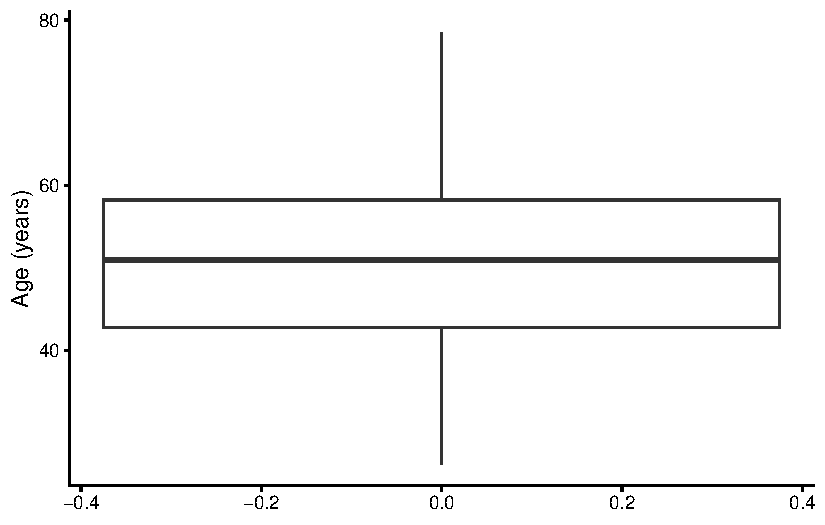
\includegraphics[keepaspectratio]{02-probability_files/figure-pdf/unnamed-chunk-38-1.pdf}}

By default, \texttt{ggplot2} includes arbitrary values on the x-axis. As
boxplots are usually constructed only for informal data investigation,
and are rarely included in formal documents, the x-axis labelling may
not be an issue. However, the x-axis labelling can be removed as
follows:

\begin{Shaded}
\begin{Highlighting}[]
\FunctionTok{ggplot}\NormalTok{(}\AttributeTok{data =}\NormalTok{ pbc, }\FunctionTok{aes}\NormalTok{(}\AttributeTok{y =}\NormalTok{ age)) }\SpecialCharTok{+}
  \FunctionTok{geom\_boxplot}\NormalTok{() }\SpecialCharTok{+}
  \FunctionTok{theme\_classic}\NormalTok{() }\SpecialCharTok{+}
  \FunctionTok{labs}\NormalTok{(}\AttributeTok{y =} \StringTok{"Age (years)"}\NormalTok{) }\SpecialCharTok{+}
  \FunctionTok{theme}\NormalTok{(}
    \AttributeTok{axis.title.x =} \FunctionTok{element\_blank}\NormalTok{(),}
    \AttributeTok{axis.text.x =} \FunctionTok{element\_blank}\NormalTok{(),}
    \AttributeTok{axis.ticks.x =} \FunctionTok{element\_blank}\NormalTok{()}
\NormalTok{  )}
\end{Highlighting}
\end{Shaded}

\pandocbounded{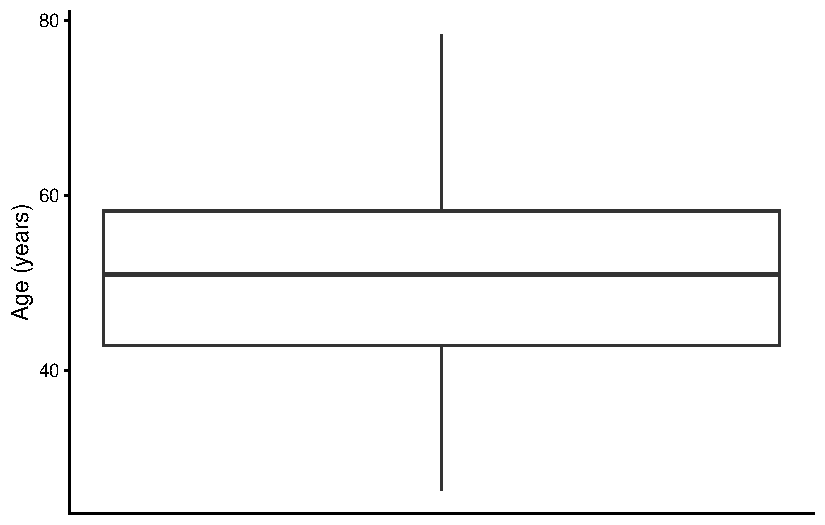
\includegraphics[keepaspectratio]{02-probability_files/figure-pdf/unnamed-chunk-39-1.pdf}}

\newpage{}

\bookmarksetup{startatroot}

\chapter*{Activities}\label{activities-1}
\addcontentsline{toc}{chapter}{Activities}

\markboth{Activities}{Activities}

\subsection*{Activity 2.1}\label{activity-2.1}
\addcontentsline{toc}{subsection}{Activity 2.1}

Researchers at a maternity hospital in the 1970s conducted a study of
low birth weight babies. Low birth weight is classified as a weight of
2500g or less at birth. Data were collected on age and smoking status of
mothers and the birth weight of their babies. The file
\texttt{Activity\_2.1.rds} contain data on the participants in the
study.

Create a 2 by 2 table to show the proportions of low birth weight babies
born to mothers who smoked during pregnancy and those that did not smoke
during pregnancy. Answer the following questions:

\begin{enumerate}
\def\labelenumi{\alph{enumi})}
\tightlist
\item
  What was the total number of mothers who smoked during pregnancy?
\item
  What proportion of mothers who smoked gave birth to low birth weight
  babies? What proportion of non-smoking mothers gave birth to low birth
  weight babies?
\item
  Construct a stacked bar chart of the data to examine if there a
  difference in the proportion of babies born with a low birth weight in
  relation to the age group of the mother? Provide appropriate labels
  for the axes and give the graph an appropriate title. {[}Hint: plot
  the data using the \texttt{AgeGrp} variable{]}
\item
  Using your answers to the question a) and b), write a brief conclusion
  about the relationship of low birth weight and mother's age and
  smoking status.
\end{enumerate}

\subsection*{Activity 2.2}\label{activity-2.2}
\addcontentsline{toc}{subsection}{Activity 2.2}

In a Randomised Controlled Trial, the preference of a new drug was
tested against an established drug by giving both drugs to each of 90
people. Assume that the two drugs are equally preferred, that is, the
probability that a patient prefers either of the drugs is equal (50\%).
Use either the web applet, or one of the binomial functions in R to
compute the probability that 60 or more patients would prefer the new
drug. In completing this question, determine:

\begin{enumerate}
\def\labelenumi{\alph{enumi})}
\tightlist
\item
  The number of trials (\texttt{n} for the web applet, \texttt{size} for
  R)
\item
  The number of successes we are interested in (\texttt{x} for web
  applet, \texttt{x} or \texttt{q} for R)
\item
  The probability of success for each trial (\texttt{p} for the web
  applet, \texttt{prob} for R)
\item
  The form of the binomial function

  \begin{itemize}
  \tightlist
  \item
    for the web applet: \texttt{P(X=x)}, \texttt{P(X≤x)} or
    \texttt{P(X≥x)};
  \item
    for R: \texttt{dbinom}, \texttt{pbinom} or
    \texttt{pbinom(lower.tail=FALSE)}
  \end{itemize}
\item
  The final probability.
\end{enumerate}

\subsection*{Activity 2.3}\label{activity-2.3}
\addcontentsline{toc}{subsection}{Activity 2.3}

A case of Schistosomiasis is identified by the detection of schistosome
ova in a faecal sample. In patients with a low level of infection, a
field technique of faecal examination has a probability of 0.35 of
detecting ova in any one faecal sample. If five samples are routinely
examined for each patient, use the web applet or R to compute the
probability that a patient with a low level of infection:

\begin{enumerate}
\def\labelenumi{\alph{enumi})}
\tightlist
\item
  Will not be identified?
\item
  Will be identified in two of the samples?
\item
  Will be identified in all the samples?
\item
  Will be identified in at most 3 of the samples?
\end{enumerate}

\subsection*{Activity 2.4}\label{activity-2.4}
\addcontentsline{toc}{subsection}{Activity 2.4}

A health survey was conducted, and an extract of data has been provided
in \texttt{Activity\_2.4-health-survey.csv}. Categorise height into 20cm
intervals, and present the height-groups appropriately.

\subsection*{Activity 2.5}\label{activity-2.5}
\addcontentsline{toc}{subsection}{Activity 2.5}

The data in the file \texttt{Activity\_2.5-LengthOfStay.rds} has
information about \textbf{birth weight} and \textbf{length of stay}
collected from 117 babies admitted consecutively to a hospital for
surgery. For each variable:

\begin{enumerate}
\def\labelenumi{\alph{enumi}.}
\item
  Plot the distribution (separately);
\item
  Complete the following summary statistics for each variable:

  \begin{itemize}
  \tightlist
  \item
    mean and median;
  \item
    standard deviation and interquartile range.
  \end{itemize}
\end{enumerate}

Make a decision about whether each variable is symmetric or not, and
which measure of central tendency and variability should be reported.

\bookmarksetup{startatroot}

\chapter{Continuous probability distributions, sampling and
precision}\label{continuous-probability-distributions-sampling-and-precision}

\section*{Learning objectives}\label{learning-objectives-2}
\addcontentsline{toc}{section}{Learning objectives}

\markright{Learning objectives}

By the end of this module you will be able to:

\begin{itemize}
\tightlist
\item
  Describe the characteristics of a Normal distribution
\item
  Compute probabilities from a Normal distribution using statistical
  software
\item
  Briefly outline other types of distributions
\item
  Explain the purpose of sampling, different sampling methods and their
  implications for data analysis
\item
  Distinguish between standard deviation of a sample and standard error
  of a mean
\item
  Calculate and interpret confidence intervals for a mean
\end{itemize}

\section*{Optional readings}\label{optional-readings-2}
\addcontentsline{toc}{section}{Optional readings}

\markright{Optional readings}

Kirkwood and Sterne (2001); Chapters 4, 5 and 6.
\href{http://er1.library.unsw.edu.au/er/cgi-bin/eraccess.cgi?url=https://ebookcentral.proquest.com/lib/unsw/detail.action?docID=624728}{{[}UNSW
Library Link{]}}

Bland (2015); Sections 3.3 and 3.4, Chapter 7, Sections 8.1 to 8.3.
\href{http://er1.library.unsw.edu.au/er/cgi-bin/eraccess.cgi?url=https://ebookcentral.proquest.com/lib/unsw/detail.action?docID=5891730}{{[}UNSW
Library Link{]}}

\section{Introduction}\label{introduction-2}

In this module, we will continue our introduction to probability by
considering probability distributions for continuous data. We will
introduce one of the most important distributions in statistics: the
Normal distribution.

To describe the characteristics of a population we can gather data about
the entire population (as is undertaken in a national census) or we can
gather data from a sample of the population. When undertaking a research
study, taking a sample from a population is far more cost-effective and
less time consuming than collecting information from the entire
population. When a sample of a population is selected, summary
statistics that describe the sample are used to make inferences about
the total population from which the sample was drawn. These are referred
to as inferential statistics.

However, for the inferences about the population to be valid, a random
sample of the population must be obtained. The goal of using random
sampling methods is to obtain a sample that is representative of the
target population. In other words, apart from random error, the
information derived from the sample is expected to be much the same as
the information collected from a complete population census as long as
the sample is large enough.

\section{Probability for continuous
variables}\label{probability-for-continuous-variables}

Calculating the probability for a categorical random variable is
relatively straightforward, as there are only a finite number of
possible events. However, there are an infinite number of possible
values for a continuous variable, and we calculate the probability that
the continuous variable lies in a range of values.

\section{Normal distribution}\label{normal-distribution}

The frequency plot for many biological and clinical measurements (for
example blood pressure and height) follow a bell shape where the curve
is symmetrical about the mean value and has tails at either end.
Figure~\ref{fig-2-1} \footnote{Source:
  https://www.aihw.gov.au/reports/risk-factors/high-blood-pressure/contents/high-blood-pressure
  (accessed March 2021)} and Figure~\ref{fig-2-2} \footnote{Source:
  https://ourworldindata.org/human-height (accessed March 2021)}
demonstrate this type of distribution.

\begin{figure}

\centering{

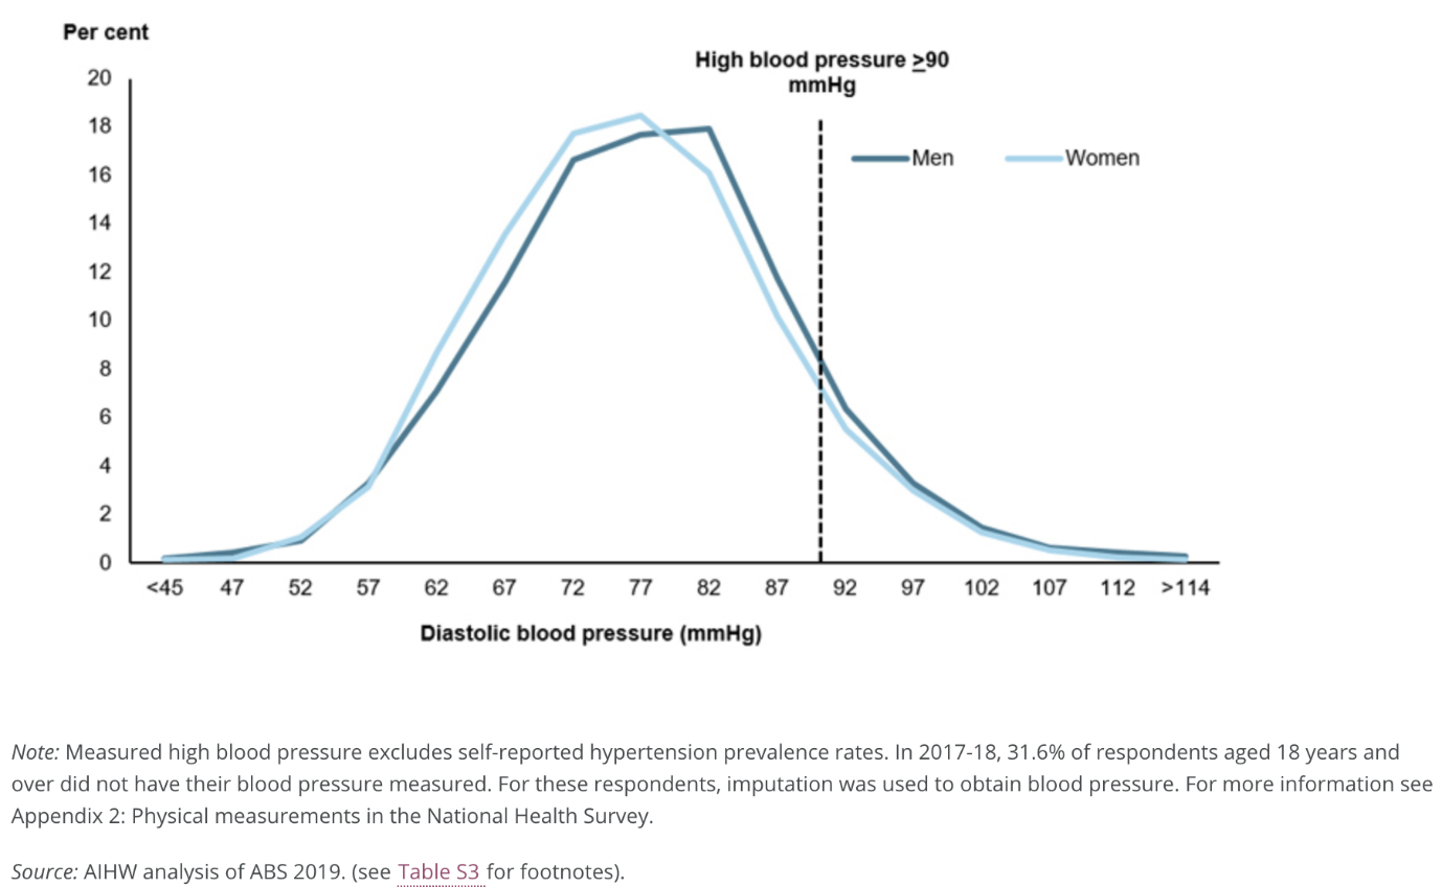
\includegraphics[width=0.66\linewidth,height=\textheight,keepaspectratio]{img/mod02/dbp.png}

}

\caption{\label{fig-2-1}Distribution of diastolic blood pressure,
2017--18 Australian Bureau of Statistics National Health Survey}

\end{figure}%

\begin{figure}

\centering{

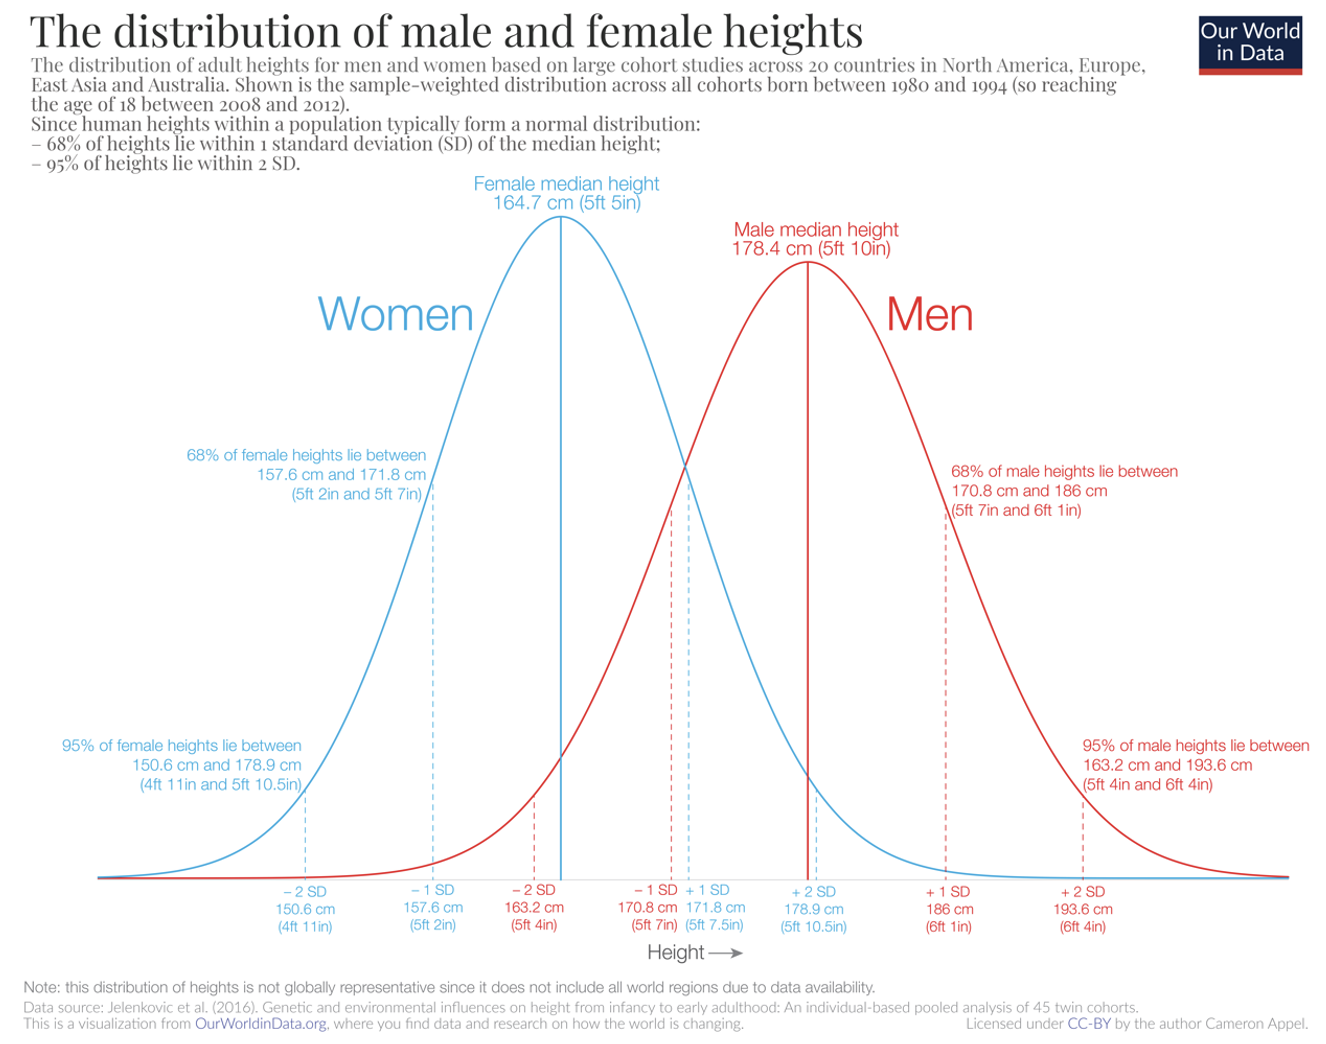
\includegraphics[width=0.66\linewidth,height=\textheight,keepaspectratio]{img/mod02/heights.png}

}

\caption{\label{fig-2-2}Distribution of male and female heights}

\end{figure}%

The Normal distribution, also called the Gaussian distribution (named
after Johann Carl Friedrich Gauss, 1777--1855), has been shown to fit
the frequency distribution of many naturally occurring variables. It is
characterised by its bell-shaped, symmetric curve and its tails that
approach zero on either side.

There are two reasons for the importance of the Normal distribution in
biostatistics (Kirkwood and Sterne, 2003). The first is that many
variables can be modelled reasonably well using the Normal distribution.
Even if the observed data were not Normally distributed, it can often be
made reasonably Normal after applying some transformation of the data.
The second (and possible most important) reason, is based on the central
limit theorem and will be discussed later in this module.

The Normal distribution is characterised by two parameters: the mean
(\(\mu\)) and the standard deviation (\(\sigma\)). The mean defines
where the middle of the Normal distribution is located, and the standard
deviation defines how wide the tails of the distribution are.

For a Normal distribution, about 68\% of the observations lie between
\(- \sigma\) and \(\sigma\) of the mean; 95\% of the observations lie
between \(−1.96 \times \sigma\) and \(1.96 \times \sigma\) from the
mean; and almost all the observations (99.7\%) lie between
\(-3 \times \sigma\) and \(3 \times \sigma\) (Figure~\ref{fig-2-3}).
Also note that the mean is the same as the median, as the curve is
symmetric about its mean.

\begin{figure}

\centering{

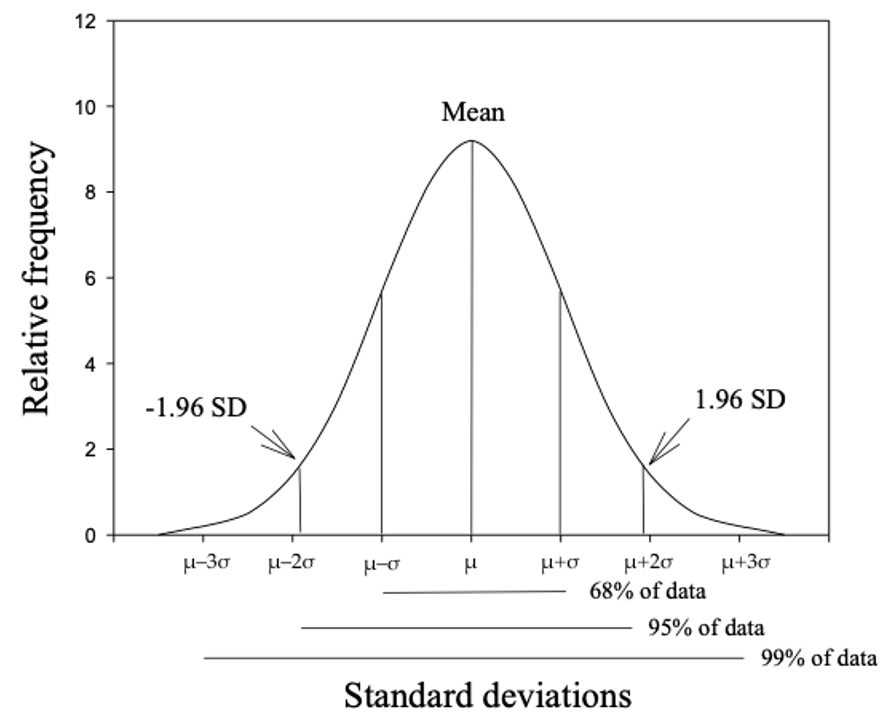
\includegraphics[width=0.66\linewidth,height=\textheight,keepaspectratio]{img/mod02/normal-curve.png}

}

\caption{\label{fig-2-3}Characteristics of a Normal distribution}

\end{figure}%

\section{The Standard Normal
distribution}\label{the-standard-normal-distribution}

As each Normal distribution is defined by its mean and standard
deviation, there are an infinite number of possible Normal
distributions. However, every Normal distribution can be transformed to
what we call the Standard Normal distribution, which has a mean of zero
(\(\mu = 0\)) and a standard deviation of one (\(\sigma = 1\)). The
Standard Normal distribution is so important that it has been assigned
its own symbol: Z.

Every observation from a Normal distribution \(X\) with a mean \(\mu\)
and a standard deviation \(\sigma\) can be transformed to a z-score
(also called a Standard Normal deviate) by the formula:

\[ z = \frac{x - \mu}{\sigma} \]

The z-score is simply how far an observation lies from the population
mean value, scaled by the population standard deviation.

We can use z-scores to estimate probabilities, as shown in Worked
Example 2.2.

\subsubsection*{Worked Example}\label{worked-example-1}
\addcontentsline{toc}{subsubsection}{Worked Example}

This example extends the example of diastolic blood pressure shown in
Figure~\ref{fig-2-1}. Assume that the mean diastolic blood pressure for
men is 77.9 mmHg, with a standard deviation of 11. What is the
probability that a man selected at random will have high blood pressure
(i.e.~diastolic blood pressure ≥ 90)?

To estimate the probability that diastolic blood pressure ≥ 90 (i.e.~the
upper tail probability), we first need to calculate the z-score that
corresponds to 90 mmHg.

Using the z-score formula, with x=90, \(\mu\)=77.9 and \(\sigma\)=11:

\[ z = \frac{90 - 77.9}{11} = 1.1 \] Thus, a blood pressure of 90 mmHg
corresponds to a z-score of 1.1, or a value 1.1 \(\times \sigma\) above
the mean weight of the population.

Figure~\ref{fig-2-5} shows the probability of a diastolic blood pressure
of 90 mmHg or more in the population for a z-score of greater than 1.1
on a Standard Normal distribution.

\begin{figure}

\centering{

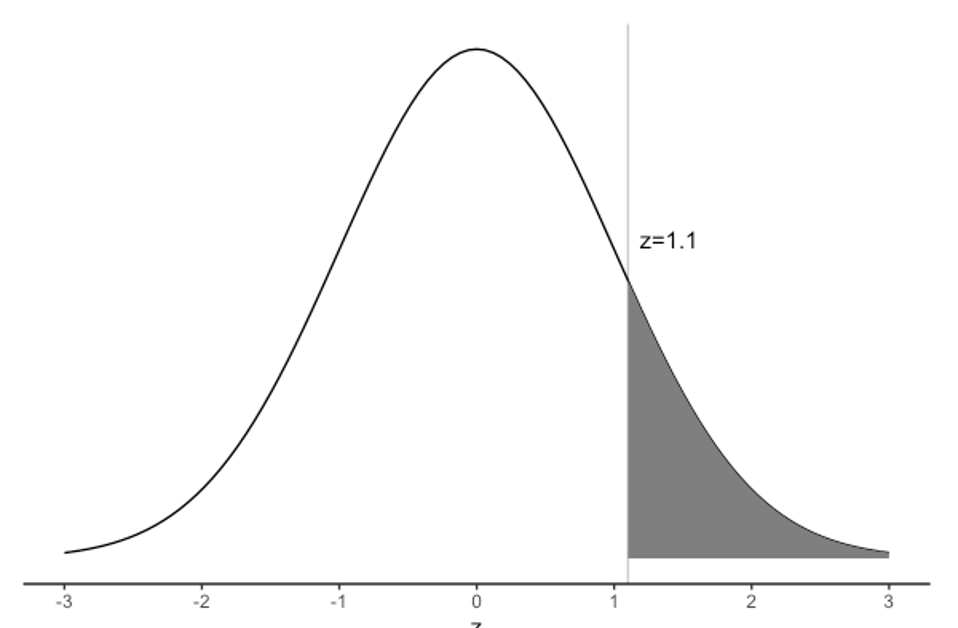
\includegraphics[width=0.66\linewidth,height=\textheight,keepaspectratio]{img/mod02/z-dist-shaded.png}

}

\caption{\label{fig-2-5}Area under the Standard Normal curve (as
probability) for Z \textgreater{} 1.1}

\end{figure}%

Using software, we find the probability that a person has a diastolic
blood pressure of 90 mmHg or more as P(Z ≥ 1.1) = 0.136.

Apart from calculating probabilities, z-scores are most useful for
comparing measurements taken from a sample to a known population
distribution. It allows measurements to be compared to one another
despite being on different scales or having different predicted values.

For example, if we take a sample of children and measure their weights,
it is useful to describe those weights as z-scores from the population
weight distribution for each age and gender. Such distributions from
large population samples are widely available. This allows us to
describe a child's weight in terms of how much it is above or below the
population average. For example, if mean weights were compared, children
aged 5 years would be on average heavier than the children aged 3 years
simply because they are older and therefore larger. To make a valid
comparison, we could use the Z-scores to say that children aged 3 years
tend to be more overweight than children aged 5 years because they have
a higher mean z-score for weight.

\section{Assessing Normality}\label{assessing-normality}

There are several ways to assess whether a continuous variable is
Normally distributed. The best way to assess whether a variable is
Normally distributed is to plot its distribution, using a density plot
for example. If the density plot looks appoximately bell-shaped and
approximately symmetrical, assuming Normality would be reasonable.

It may be useful to examine a boxplot of a variable in conjunction with
a density plot. However a boxplot in isolation is not as useful as a
density plot, as a boxplot only indicates whether a variable is
distributed symmetrically (indicated by equal ``whiskers''). A boxplot
cannot give an indication of whether the distribution is bell-shaped, or
flat.

\begin{quote}
For your information: There are formal tests that test for Normality.
These tests are beyond the scope of this course and are not recommended.
\end{quote}

We can construct a density plot for \texttt{age} in the \texttt{pbc}
data introduced in Module 1. We can see that the density plot is
approximately approximately bell-shaped and roughly symmetrical. The
mean (50.7 years) and median (51 years) are similar, as would be
expected for a Normal distribution. Thus, it would be reasonable to
assume that age is Normally distributed in this set of data.

\begin{figure}

\centering{

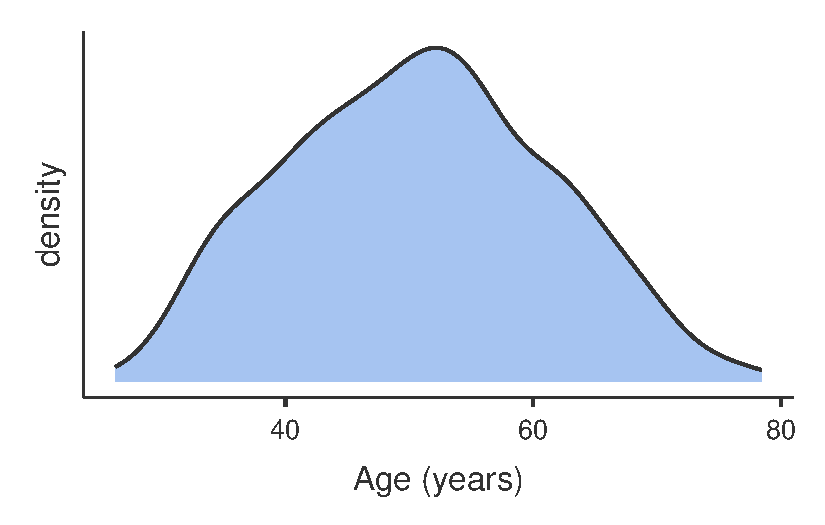
\includegraphics[width=0.5\linewidth,height=\textheight,keepaspectratio]{03-precision_files/figure-pdf/fig-age-pbc-1.pdf}

}

\caption{\label{fig-age-pbc}Density plot of participant age from PBC
study data}

\end{figure}%

\section{Non-Normally distributed
measurements}\label{non-normally-distributed-measurements}

Not all measurements are Normally distributed, and the symmetry of the
bell shape may be distorted by the presence of some very small or very
large values. Non-Normal distributions such as this are called skewed
distributions.

When there are some very large values, the distribution is said to be
positively skewed.This often occurs when measuring variables related to
time, such as days of hospital stay, where most patients have short
stays (say 1 - 5 days) but a few patients with serious medical
conditions have very long lengths of hospital stay (say 20 - 100 days).

In practice, most parametric summary statistics are quite robust to
minor deviations from Normality and non-parametric statistical methods
are only required when the sample size is small and/or the data are
obviously skewed with some influential outliers.

When the data are markedly skewed, density plots are not all
bell-shaped. For example, serum bilirubin measured from participants in
the PBC study are presented in Figure~\ref{fig-bili-pbc}.

\begin{figure}

\centering{

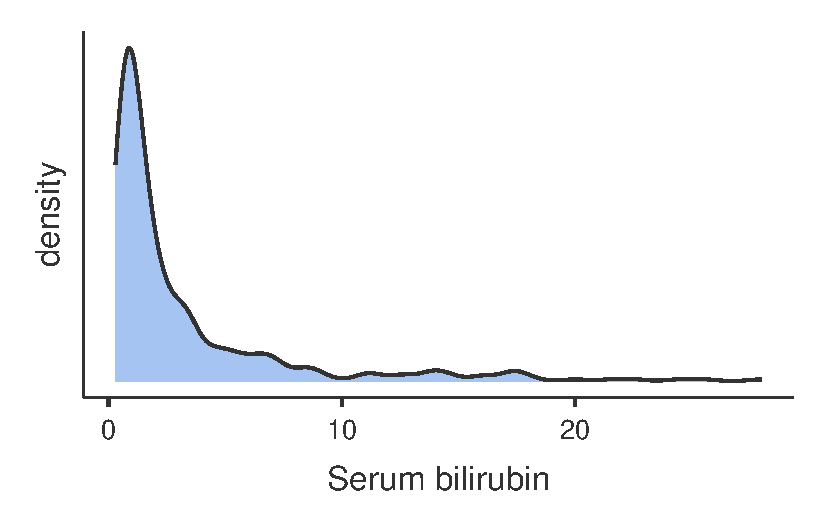
\includegraphics[width=0.5\linewidth,height=\textheight,keepaspectratio]{03-precision_files/figure-pdf/fig-bili-pbc-1.pdf}

}

\caption{\label{fig-bili-pbc}Density plot of serum bilirubin from PBC
study data}

\end{figure}%

In the plot of c, there is a tail of values to the right, so we would
conclude that the distribution is skewed to the right. The mean (3.2
mg/dL) is much larger than the median (1.4 mg/dL), as expected from a
skewed distribution.

\section{Parametric and non-parametric statistical
methods}\label{parametric-and-non-parametric-statistical-methods}

Many statistical methods are based on assumptions about the distribution
of the variable -- these methods are known as parametric statistical
methods. Many methods of statistical inferences based on theoretical
sampling properties that are derived from a Normal distribution with the
characteristics described above. Thus, it is important that measurements
approximate to a Normal distribution before these parametric methods are
used. The methods are called `parametric' because they are based on the
parameters -- the mean and standard deviation - that underlie a Normal
distribution. Statistics which do not assume a particular distribution
are called distribution-free statistics, or `non-parametric statistics'.

In this course, you will learn about both parametric and non-parametric
statistical methods. Parametric summary statistical methods include
those based on the mean, standard deviation and range (Module 1), and
standard error and 95\% confidence interval (Module 3). Parametric
statistical tests also include t-tests which will be covered in Modules
4 and 5, and correlation and regression described in Module 8.

Non-parametric summary statistical methods are often based on ranks, and
may use such statistics as the median, mode and inter-quartile range
(Module 1). Non-parametric statistical tests that use ranking are
described in Module 9.

\section{Other types of probability
distributions}\label{other-types-of-probability-distributions}

In this module we have considered a Normal probability distribution and
how to use it to measure the precision of continuously distributed
measurements. Data also follow other types of distributions which are
briefly described below. In other modules in this course, we will be
looking at a range of methods to analyse health data and will refer back
to these different distributions.

Normal approximation of binomial: When the sample size becomes large, it
becomes cumbersome to calculate the exact probability of an event using
the binomial distribution. Conveniently, with large sample sizes, the
binomial distribution approximates a Normal distribution. The mean and
SD of a binomial distribution can be used to calculate the probability
of the event as though it was from a Normal distribution.

Poisson distribution: is another distribution which is often used in
health research for modelling count data. The Poisson distribution is
followed when a number of events happen in a fixed time interval. This
distribution is useful for describing data such as deaths in the
population in a time period. For example, the number of deaths from
breast cancer in one year in women over 50 years old will be an
observation from a Poisson distribution. We can also use this to make
comparisons of mortality rates between populations.

Many other probability distributions can be derived for functions which
arise in statistical analyses but the chi-squared, t and F distributions
are the three distributions that are most widely used. These have many
applications, some of which are described in later modules.

The chi-squared distribution is a skewed distribution which allows us to
determine the probability of a deviation between a count that we observe
and a count that we expect for categorical data. One use of this is in
conducting statistical tests for categorical data. See Module 7.

A t-distribution is used when the population standard deviation is not
known. The t-distribution is appropriate for small samples (\textless30)
and its distribution is bell shaped similar to a Normal distribution but
slightly flatter. The t-distribution is useful for comparing mean
values. See Module 4 and Module 5.

\section{Sampling methods}\label{sampling-methods}

Methods have been designed to select participants from a population such
that each person in the target population has an equal probability of
being chosen. Methods that use this approach are called random sampling
methods. Examples include simple random sampling and stratified random
sampling.

In simple random sampling, every person in the population from which the
sample is drawn has the same random chance of being selected into the
sample. To implement this method, every person in the population is
allocated an ID number and then a random sample of the ID numbers is
selected. Software packages can be used to generate a list of random
numbers to select the random sample.

In stratified sampling, the population is divided into distinct
non-overlapping subgroups (strata) according to an important
characteristic (e.g.~age or sex) and then a random sample is selected
from each of the strata. This method is used to ensure that sufficient
numbers of people are sampled from each stratum and therefore each
subgroup of interest is adequately represented in the sample.

The purpose of using random sampling is to minimise selection bias to
ensure that the sample enrolled in a study is representative of the
population being studied. This is important because the summary
statistics that are obtained can then be regarded as valid in that they
can be applied (generalised) back to the population.

A non-representative sample might occur when random sampling is used,
simply by chance. However, non-random sampling methods, such as using a
study population that does not represent the whole population, will
often result in a non-representative sample being selected so that the
summary statistics from the sample cannot be generalised back to the
population from which the participants were drawn. The effects of
non-random error are much more serious than the effects of random error.
Concepts such as non-random error (i.e.~systematic bias), selection
bias, validity and generalisability are discussed in more detail in
PHCM9794: Foundations of Epidemiology.

\section{Standard error and
precision}\label{standard-error-and-precision}

Module 1 introduced the mean, variance and standard deviation as
measures of central tendency and spread for continuous measurements from
a sample or a population. As described in Module 1, we rarely have data
on the entire population but we \emph{infer} information \emph{about}
the population from a \emph{sample}. For example, we use the sample mean
\(\bar x\) as an \emph{estimate} of the true population mean \(\mu\).

However, a sample taken from a population is usually a small proportion
of the total population. If we were to take multiple samples of data and
calculate the sample mean for each sample, we would not expect them to
be identical. If our samples were very small, we would not be surprised
if our estimated sample means were somewhat different from each other.
However, if our samples were large, we would expect the sample means to
be less variable, i.e.~the estimated sample means would be more close to
each other, and hopefully, to the true population mean.

\subsection{The standard error of the mean}\label{sec-semean}

A point estimate is a single best guess of the true value in the
population - taken from our sample of data. Different samples will
provide slightly different point estimates. The standard error is a
measure of variability of the point estimate.

In particular, the \emph{standard error of the mean} measures the extent
to which we expect the means from different samples to vary because of
chance due to the sampling process. This statistic is directly
proportional to the standard deviation of the variable, and inversely
proportional to the size of the sample. The standard error of the mean
for a continuously distributed measurement for which the SD is an
accurate measure of spread is computed as follows:

\[ \text{SE}(\bar{x}) = \frac{\text{SD}}{\sqrt{n}} \]

\subsection{Worked Example 3.1: blood pressure of Pima
women}\label{worked-example-3.1-blood-pressure-of-pima-women}

The diastolic blood pressure of 733 female Pima indigenous Americans was
measured, and a density plot produced (Figure~\ref{fig-dbp-pima}). These
data are saved as \texttt{mod03\_blood\_pressure.csv}.

\begin{figure}

\centering{

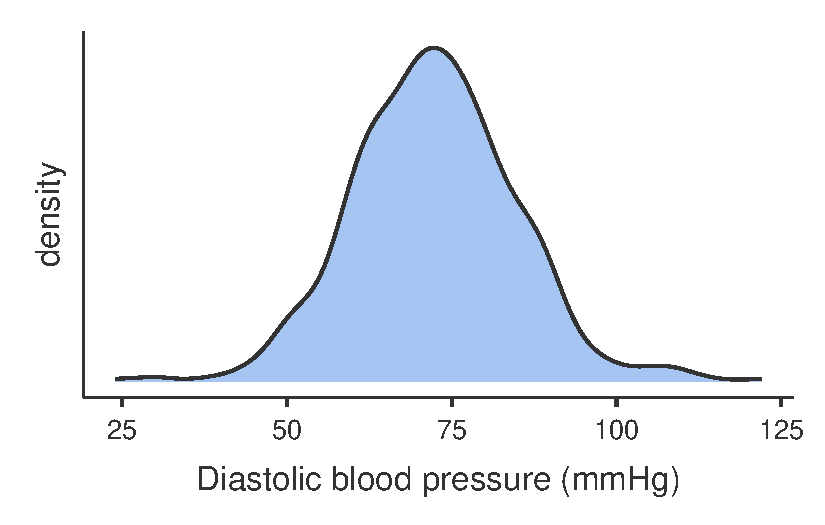
\includegraphics[width=0.5\linewidth,height=\textheight,keepaspectratio]{03-precision_files/figure-pdf/fig-dbp-pima-1.pdf}

}

\caption{\label{fig-dbp-pima}Density plot of diastolic blood pressure
from 733 Pima indigenous American women}

\end{figure}%

The density plot shows that diastolic blood pressure is approximately
normally distributed. The mean diastolic blood pressure in the sample
was 72.4 mmHg with a standard deviation of 12.38 mmHg.

Hence, the standard error of the mean is estimated as:

\[ \text{SE}(\bar{x}) = \frac{12.38}{\sqrt{733}} = 0.457 \]

Because the calculation uses the sample size (n) (i.e.~the number of
study participants) in the denominator, the SE will become smaller when
the sample size becomes larger. A smaller SE indicates that the
estimated mean value is more precise.

The standard error is an important statistic that is related to sampling
variation. When a random sample of a population is selected, it is
likely to differ in some characteristic compared with another random
sample selected from the same population. Also, when a sample of a
population is taken, the true population mean is an unknown value.

Just as the standard deviation measures the spread of the data around
the population mean, the standard error of the mean measures the spread
of the sample means. Note that we do not have different samples, only
one. It is a theoretical concept which enables us to conduct various
other statistical analyses.

\section{Data sovereignty: can data be
owned?}\label{data-sovereignty-can-data-be-owned}

Data sovereignty proclaims the right of peoples to govern the
collection, ownership and application of their own data. Data
sovereignty recognises data not only as information, but as a cultural
and economic asset that holds value for the communities it represents.

The principle of data sovereignty advocates strongly for data rights and
interests, emphasising that data must be used in ways that support and
enhance the collective well-being of the communities from which it
collected. A critical aspect of this framework is the avoidance of
exploitative research practices, ensuring that research is conducted
\emph{by} or \emph{with} communities rather than simply \emph{on} them.
This participatory approach recognises communities as active members in
the research process rather than passive subjects of study.

\subsection{The Pima Indian Diabetes
Dataset}\label{the-pima-indian-diabetes-dataset}

The importance of data sovereignty principles is highlighted by the Pima
Indian Diabetes Dataset (PIDD). The Pima people, living in Arizona USA,
are known for high rates of diabetes and obesity. In 1965, the United
States National Institutes of Health began an observational study of the
Pima community, viewing their reservation as a ``natural laboratory''
for diabetes research. Originally planned to last ten years, this study
continued for approximately forty years, collecting highly personal
information including blood pressure, body mass index, and number of
pregnancies of Pima Americans.

The data collected during this study became known as the Pima Indian
Diabetes Dataset and was subsequently included in the University of
California, Irvine (UCI) Machine Learning Repository.(University of
California Irvine, n.d.) This repository, established in 1987, is a
collection of datasets and tools used to test and train machine learning
models. Although the PIDD appears to have been removed from the UCI
repository, it now appears in major machine learning repositories such
as Kaggle. Significantly, this dataset has been used to refine
algorithms intended for ``knowledge discoveries'' that have nothing to
do with diabetes, including the prediction of manhole fires.

This case raises profound questions about what might be termed ``eternal
consent.'' The Pima participants who provided their medical data in 1965
could not have realistically been informed of all potential uses for
their medical data forty years into the future. The transformation of
intimate health data, collected for a specific diabetes research
purpose, into a widely distributed dataset for training machine learning
algorithms represents a fundamental breach of the principles of data
sovereignty. The Pima community had no control over the secondary uses
of their data, no ongoing governance role, and no ability to determine
whether these uses aligned with their collective well-being or cultural
values. This example demonstrates the critical need for robust data
sovereignty frameworks that protect Indigenous peoples' rights to
control not only the initial collection of their data but also its
subsequent use, storage, and dissemination.

\section{Central limit theorem}\label{central-limit-theorem}

Even though we now have an estimate of the mean and its standard error,
we might like to know what the mean from a different random sample of
the same size might be. To do this, we need to know how sample means are
distributed. In determining the form of the probability distribution of
the sample mean (\(\bar{x}\)), we consider two cases:

\subsection{When the population distribution is
unknown:}\label{when-the-population-distribution-is-unknown}

The central limit theorem for this situation states:

\begin{quote}
In selecting random samples of size \(n\) from a population with mean
\(\mu\) and standard deviation \(\sigma\), the sampling distribution of
the sample mean \(\bar{x}\) approaches a normal distribution with mean
\(\mu\) and standard deviation \(\tfrac{\sigma}{\sqrt{n}}\) as the
sample size becomes large.
\end{quote}

The sample size n = 30 and above is a rule of thumb for the central
limit theorem to be used. However, larger sample sizes may be needed if
the distribution is highly skewed.

\subsection{When the population is assumed to be
normal:}\label{when-the-population-is-assumed-to-be-normal}

\begin{quote}
In this case the sampling distribution of \(\bar{x}\) is normal for any
sample size.
\end{quote}

\section{95\% confidence interval of the
mean}\label{confidence-interval-of-the-mean}

Earlier, we showed that the characteristics of a Standard Normal
Distribution are that 95\% of the data lie within 1.96 standard
deviations from the mean (Figure~\ref{fig-2-2}). Because the central
limit theorem states that the sampling distribution of the mean is
approximately Normal in large enough samples, we expect that 95\% of the
sample mean values would fall within 1.96 × SE units above and below the
true mean population value.

For example, if we took 100 different random samples from the population
of Pima women and calculated the mean diastolic blood pressure for each
of the 100 samples, approximately 95\% of these sample means would fall
within 1.96 × SE of the population mean weight.

This interpretation of the SE is translated into the concept of
precision as a 95\% confidence interval. A 95\% confidence interval is a
range of values within which we have 95\% confidence that the true
population mean lies. If repeated samples were taken a very large number
of times, and a 95\% confidence interval was calculated for each sample,
95\% of the confidence intervals would contain the true population mean.

The calculation of the 95\% confidence interval for a mean is as
follows:

\[  \bar{x} \pm 1.96 \times \text{SE}( \bar{x} ) \] This is the generic
formula for calculating 95\% CI for any summary statistic. In general,
the mean value can be replaced by the point estimate of a rate or a
proportion and the same formula applies for computing 95\% CIs, i.e.

\[ 95\% \text{ CI} = \text{point estimate} \pm 1.96 \times \text{SE}(\text{point estimate)} \]

The main difference in the methods used to calculate the 95\% CI for
different point estimates is the way the SE is calculated. The methods
for calculating 95\% CI around proportions and other ratio measures will
be discussed in Module 6.

The use of 1.96 as a general critical value to compute the 95\% CI is
determined by sampling theory. For the confidence interval of the mean,
the critical value (1.96) is based on normal distribution (true when the
population SD is known). However, in practice, statistical packages will
provide slightly different confidence intervals because they use a
critical value obtained from the t-distribution. The t-distribution
approaches a normal distribution when the sample size approaches
infinity, and is close to a normal distribution when the sample size is
≥30.The critical values obtained from the t-distribution are always
larger than the corresponding critical value from the normal
distribution. The difference gets smaller as the sample size becomes
larger. For example, when the sample size n=10, the critical value from
the t-distribution is 2.26 (rather than 1.96); when n= 30, the value is
2.05; when n=100, the value is 1.98; and when n=1000, the critical value
is 1.96.

The critical value multiplied by SE (for normal distribution, 1.96 × SE)
is called the maximum likely error for 95\% confidence.

\subsection{The t-distribution and when should I use
it?}\label{the-t-distribution-and-when-should-i-use-it}

The population standard deviation (\(\sigma\)) is required for
calculation of the standard error. Usually, \(\sigma\) is not known and
the sample standard deviation (\(s\)) is used to estimate it. It is
known, however, that the sample standard deviation of a normally
distributed variable underestimates the true value of \(\sigma\),
particularly when the sample size is small.

Someone by the pseudonym of Student came up with the Student's t
distribution with (\(n-1\)) degrees of freedom to account for this
underestimation. It looks very much like the standardised normal
distribution, only that it has fatter tails
(Figure~\ref{fig-mod03-z-t-dist}). As the degrees of freedom increase
(i.e.~as \(n\) increases), the t-distribution gradually approaches the
standard normal distribution. With a sufficiently large sample size, the
Student's t-distribution closely approximates the standardised normal
distribution.

\begin{figure}

\centering{

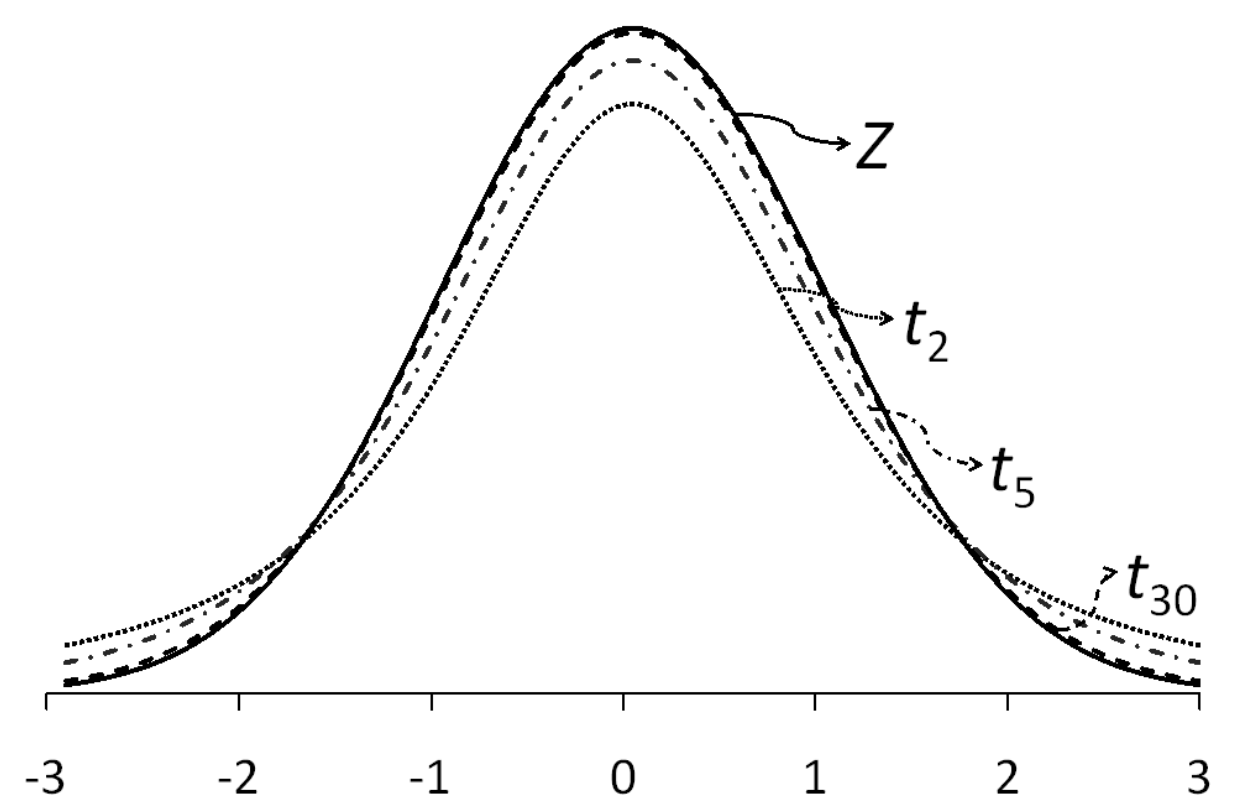
\includegraphics[width=0.5\linewidth,height=\textheight,keepaspectratio]{img/mod03/mod03-z-t-dist.png}

}

\caption{\label{fig-mod03-z-t-dist}The normal (Z) and the student's
t-distribution with 2, 5 and 30 degrees of freedom}

\end{figure}%

If a variable \(X\) is normally distributed and the population standard
deviation \(\sigma\) is known, using the normal distribution is
appropriate. However, if \(\sigma\) is not known then one should use the
student t-distribution with (\(n – 1\)) degrees of freedom.

\subsection{Worked Example 3.2: blood pressure of Pima
women}\label{worked-example-3.2-blood-pressure-of-pima-women}

Using our example of diastolic blood pressure measured from 733 female
Pima indigenous Americans, we can use software to calculate the mean,
its standard error, and the 95\% confidence interval of the mean:

\begin{longtable}[]{@{}
  >{\raggedright\arraybackslash}p{(\linewidth - 8\tabcolsep) * \real{0.1806}}
  >{\raggedright\arraybackslash}p{(\linewidth - 8\tabcolsep) * \real{0.1806}}
  >{\raggedright\arraybackslash}p{(\linewidth - 8\tabcolsep) * \real{0.1806}}
  >{\raggedright\arraybackslash}p{(\linewidth - 8\tabcolsep) * \real{0.1806}}
  >{\raggedright\arraybackslash}p{(\linewidth - 8\tabcolsep) * \real{0.2778}}@{}}
\caption{Summary of blood pressure from female Pima indigenous
Americans}\label{tbl-mean-ci}\tabularnewline
\toprule\noalign{}
\begin{minipage}[b]{\linewidth}\raggedright
n
\end{minipage} & \begin{minipage}[b]{\linewidth}\raggedright
Mean
\end{minipage} & \begin{minipage}[b]{\linewidth}\raggedright
Standard deviation
\end{minipage} & \begin{minipage}[b]{\linewidth}\raggedright
Standard error of the mean
\end{minipage} & \begin{minipage}[b]{\linewidth}\raggedright
95\% confidence interval of the mean
\end{minipage} \\
\midrule\noalign{}
\endfirsthead
\toprule\noalign{}
\begin{minipage}[b]{\linewidth}\raggedright
n
\end{minipage} & \begin{minipage}[b]{\linewidth}\raggedright
Mean
\end{minipage} & \begin{minipage}[b]{\linewidth}\raggedright
Standard deviation
\end{minipage} & \begin{minipage}[b]{\linewidth}\raggedright
Standard error of the mean
\end{minipage} & \begin{minipage}[b]{\linewidth}\raggedright
95\% confidence interval of the mean
\end{minipage} \\
\midrule\noalign{}
\endhead
\bottomrule\noalign{}
\endlastfoot
733 & 72.4 & 12.38 & 0.46 & 71.5 to 73.3 \\
\end{longtable}

We can interpret this confidence interval as: we are 95\% confident that
the true mean diastolic blood pressure of female Pima indigenous
Americans lies between 71.5 and 73.3 mmHg.

\subsection{Worked Example 3.2: 95\% CI of a mean using summarised
data}\label{worked-example-3.2-95-ci-of-a-mean-using-summarised-data}

The publication of a study using a sample of 242 participants reported a
sample mean systolic blood pressure of 128.4 mmHg and a sample standard
deviation of 19.56 mmHg. Find the 95\% confidence interval for the mean
systolic blood pressure.

Using jamovi or R, we obtain a 95\% confidence interval from 125.9232 to
130.8768.

We are 95\% confident that the true mean systolic blood pressure of the
population from which the sample was drawn lies between 125.9 kg and
130.9 mmHg.

\newpage{}

\bookmarksetup{startatroot}

\chapter*{Jamovi notes}\label{jamovi-notes-1}
\addcontentsline{toc}{chapter}{Jamovi notes}

\markboth{Jamovi notes}{Jamovi notes}

\section{Generating new variables}\label{generating-new-variables}

We commonly need to create new variables based on existing variables in
our data. For example, body size is often summarised using the
\textbf{Body Mass Index (BMI)}. BMI is calculated as:
\(\frac{\text{weight (kg)}}{\text{height (m)}^2}\).

In this demonstration, we will import a selection of records from a
large health survey, stored in the file
\texttt{mod03\_health\_survey.xlsx}. The health survey data contains
1140 records, comprising:

\begin{itemize}
\tightlist
\item
  sex: 1 = respondent identifies as male; 2 = respondent identifies as
  female
\item
  height: height in meters
\item
  weight: weight in kilograms
\end{itemize}

To generate a new variable, we use \textbf{Data \textgreater{} Compute}:

\begin{enumerate}
\def\labelenumi{\arabic{enumi}.}
\tightlist
\item
  click \textbf{Data} to open the spreadsheet, and click into an empty
  column
\item
  click \textbf{Setup} then \textbf{NEW COMPUTED VARIABLE}
\item
  enter the name of the new variable, here \texttt{BMI}
\item
  in the formula (*f\textsubscript{x}) box enter:
  \texttt{weight\ /\ height\^{}2} (note: \^{}2 represents ``to the power
  of 2'', or ``squared'')
\end{enumerate}

You should check the construction of any new variable buy examining a
density plot and/or a boxplot:

\begin{figure}

\begin{minipage}[t]{0.50\linewidth}

\raisebox{-\height}{

\pandocbounded{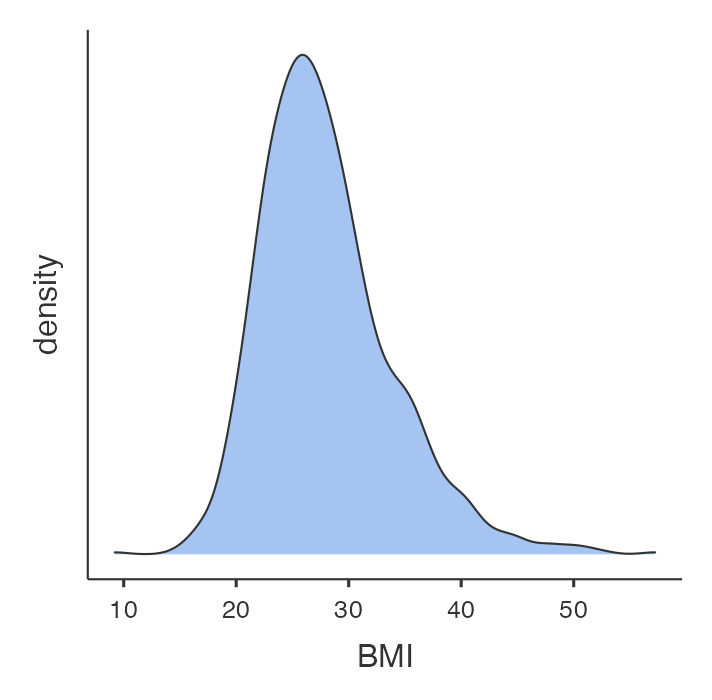
\includegraphics[keepaspectratio]{img/mod03/jamovi/mod03-newvar-dens.png}}

}

\end{minipage}%
%
\begin{minipage}[t]{0.50\linewidth}

\raisebox{-\height}{

\pandocbounded{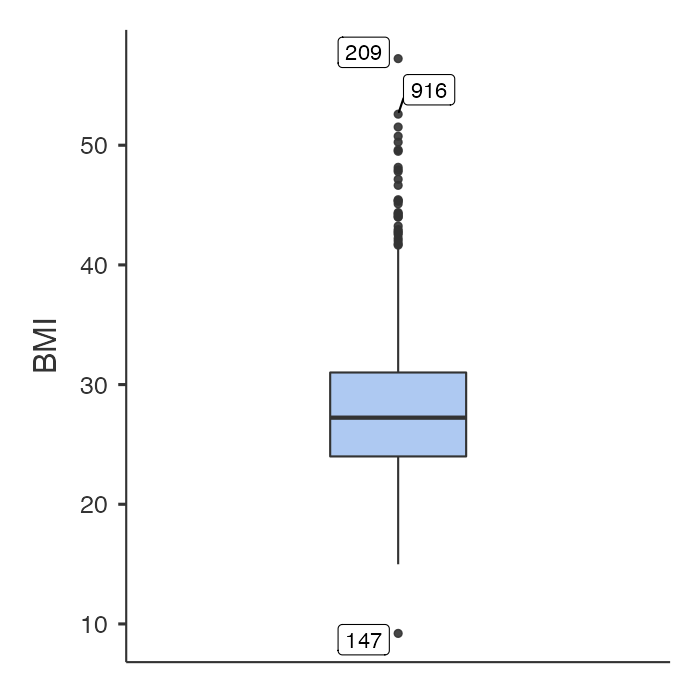
\includegraphics[keepaspectratio]{img/mod03/jamovi/mod03-newvar-boxp.png}}

}

\end{minipage}%

\end{figure}%

In the general population, BMI ranges between about 15 to 30. It appears
that BMI has been correctly generated in this example, perhaps with some
unsual values that might require investigation.

\section{Summarising data by another
variable}\label{summarising-data-by-another-variable}

We will often want to calculate the same summary statistics by another
variable. For example, we might want to calculate summary statistics for
BMI for males and females separately. We can do this in jamovi by
defining sex as a \emph{by-variable}.

This can be done easily in jamovi by defining a \textbf{Split by}
variable. For example, to summarise BMI for males and females
separately, we use \texttt{sex} as the Split by variable:

\pandocbounded{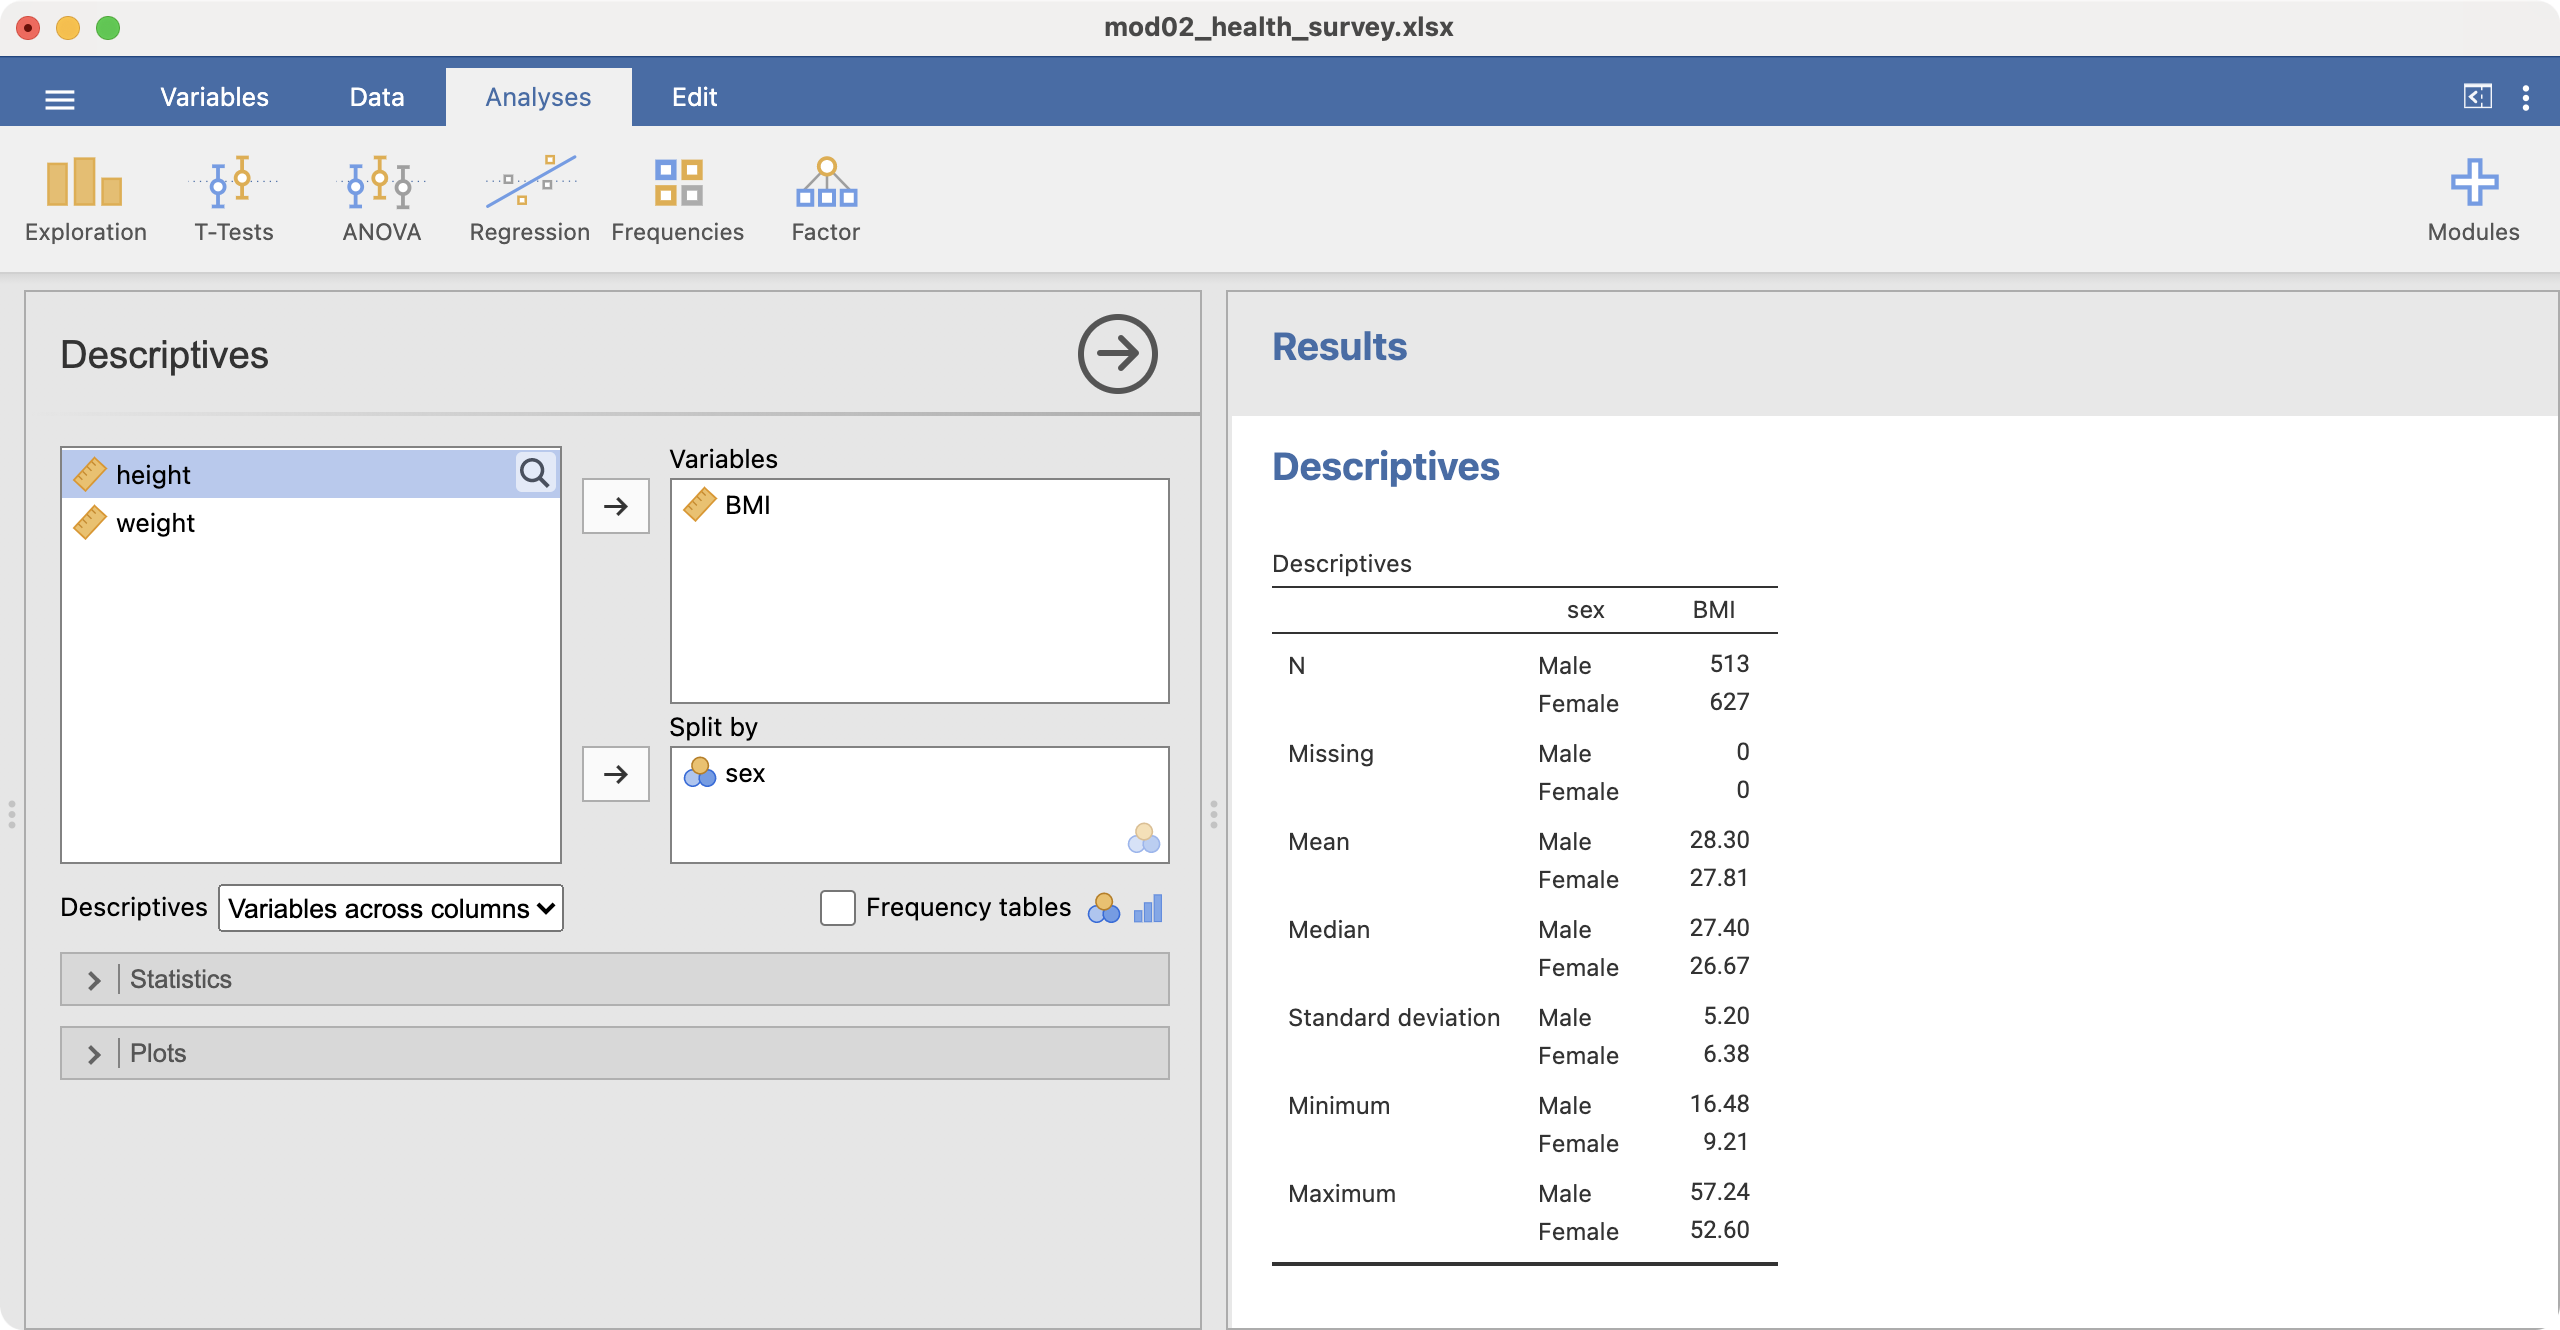
\includegraphics[keepaspectratio]{img/mod03/jamovi/mod03-splitby.png}}

\begin{figure}

\begin{minipage}[t]{0.50\linewidth}

\raisebox{-\height}{

\pandocbounded{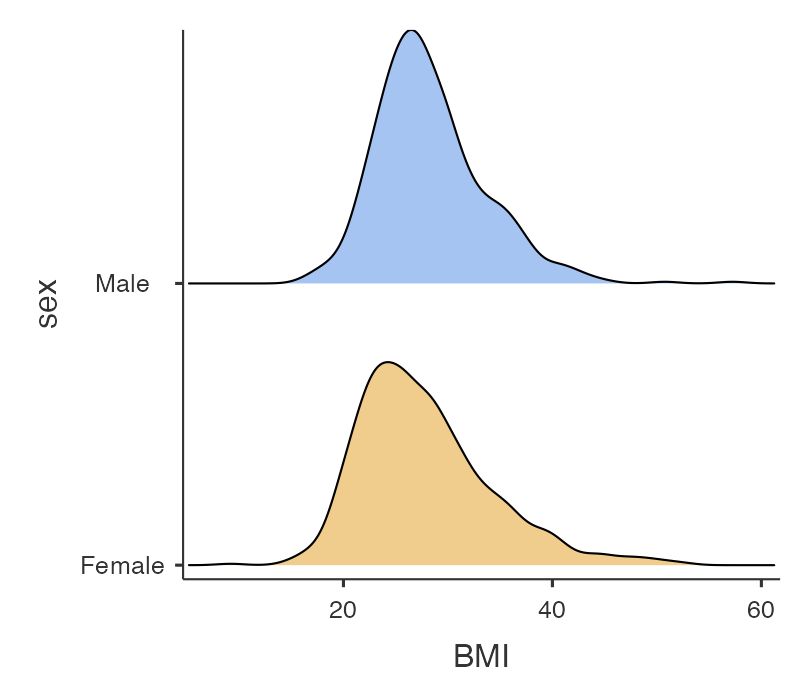
\includegraphics[keepaspectratio]{img/mod03/jamovi/mod03_splitby_dens.png}}

}

\end{minipage}%
%
\begin{minipage}[t]{0.50\linewidth}

\raisebox{-\height}{

\pandocbounded{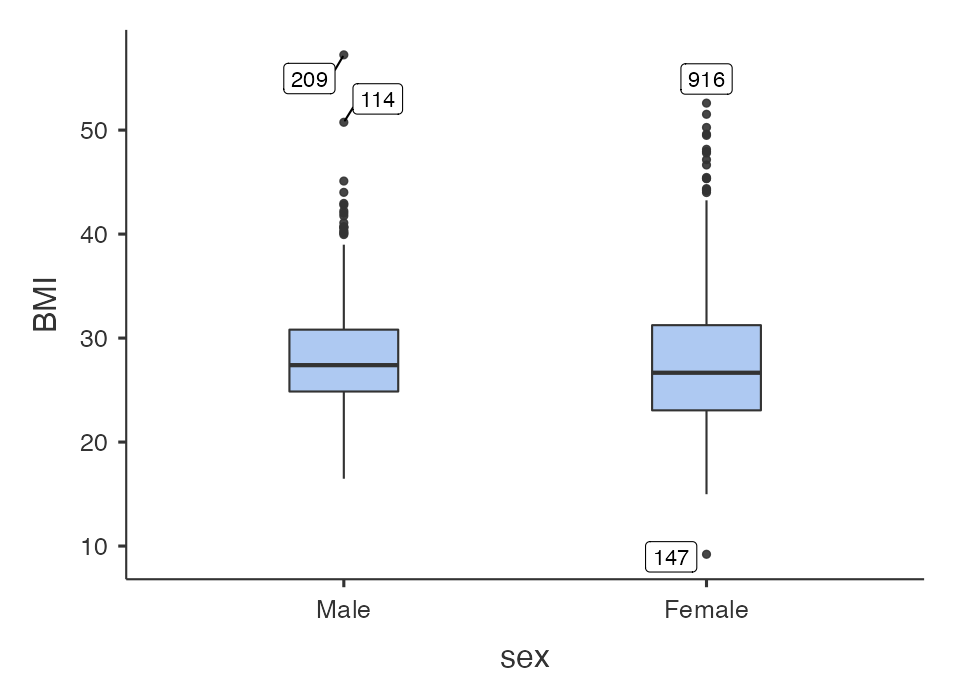
\includegraphics[keepaspectratio]{img/mod03/jamovi/mod03_splitby_boxp.png}}

}

\end{minipage}%

\end{figure}%

\section{Computing probabilities from a Normal
distribution}\label{sec-normal-jamovi}

jamovi does not have a point-and-click method for computing
probabilities from a Normal distribution. Here, instructions are
provided for using a third-party applet. This Normal Distribution Applet
has been posted at \url{https://mabognar.github.io/apps/normal.html},
and provides a simple and intuitive way to compute probabilities from a
Normal distribution. The applet requires three pieces of information:

\begin{itemize}
\tightlist
\item
  \(\mu\): the mean of the Normal distribution being considered
\item
  \(\sigma\): the standard deviation of the Normal distribution being
  considered
\item
  \(x\): the value being considered
\end{itemize}

We also need to consider whether we are interested in the probability
being greater than x, or less than x.

For example, to obtain the probability of obtaining 0.5 or greater from
a standard normal (i.e.~\(/mu\)=0, \(/sigma\)=1) distribution:

\pandocbounded{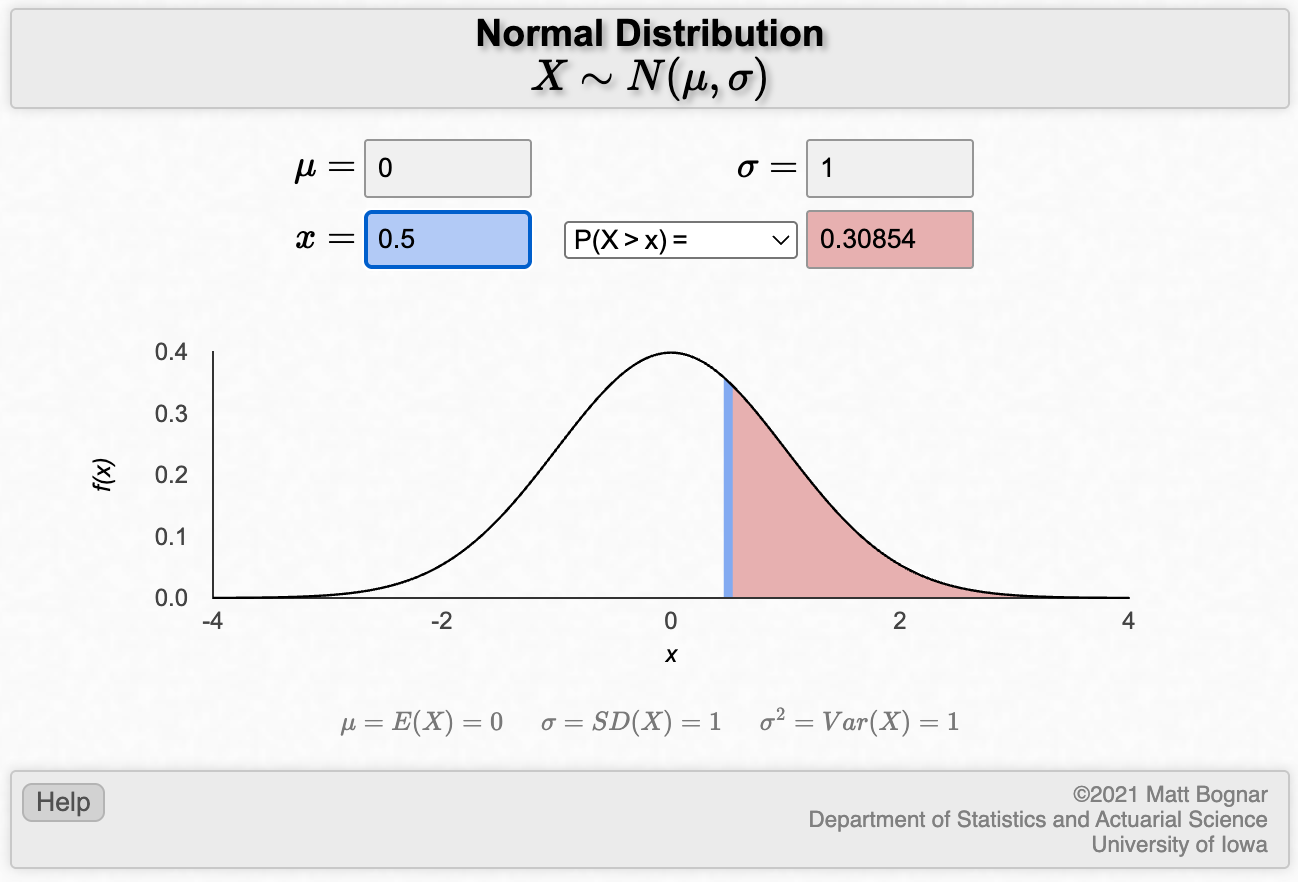
\includegraphics[keepaspectratio]{img/mod03/jamovi/mod03-norm01.png}}

The Normal curve of interest is shaded, and the probability is provided
as 0.30854.

To calculate the worked example: Assume that the mean diastolic blood
pressure for men is 77.9 mmHg, with a standard deviation of 11. What is
the probability that a man selected at random will have high blood
pressure (i.e.~diastolic blood pressure greater than or equal to 90)?

\pandocbounded{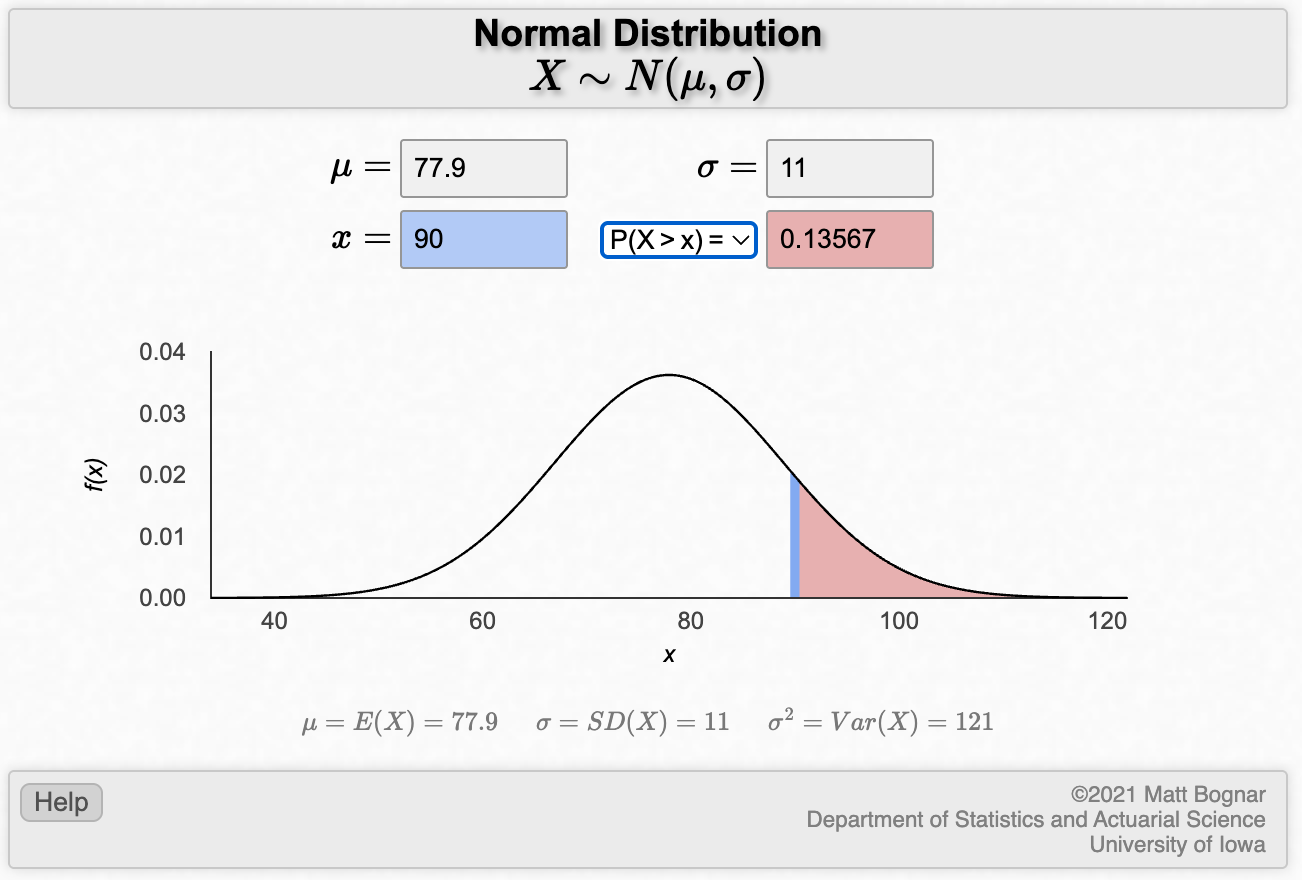
\includegraphics[keepaspectratio]{img/mod03/jamovi/mod03-norm02.png}}

\section{Calculating a 95\% confidence interval of a mean: Individual
data}\label{sec-cimean-jamovi-ind}

To demonstrate the computation of the 95\% confidence interval of a
mean, we can use the data from \texttt{mod03\_blood\_pressure.csv}. We
can use \textbf{Exploration \textgreater{} Descriptives} to calculate
the mean, its standard error and the 95\% confidence interval for the
mean. Choose \textbf{dbp} as the analysis variable, and select
\textbf{Std. error of Mean} and \textbf{Confidence interval for Mean} in
the \textbf{Statistics} section:

\pandocbounded{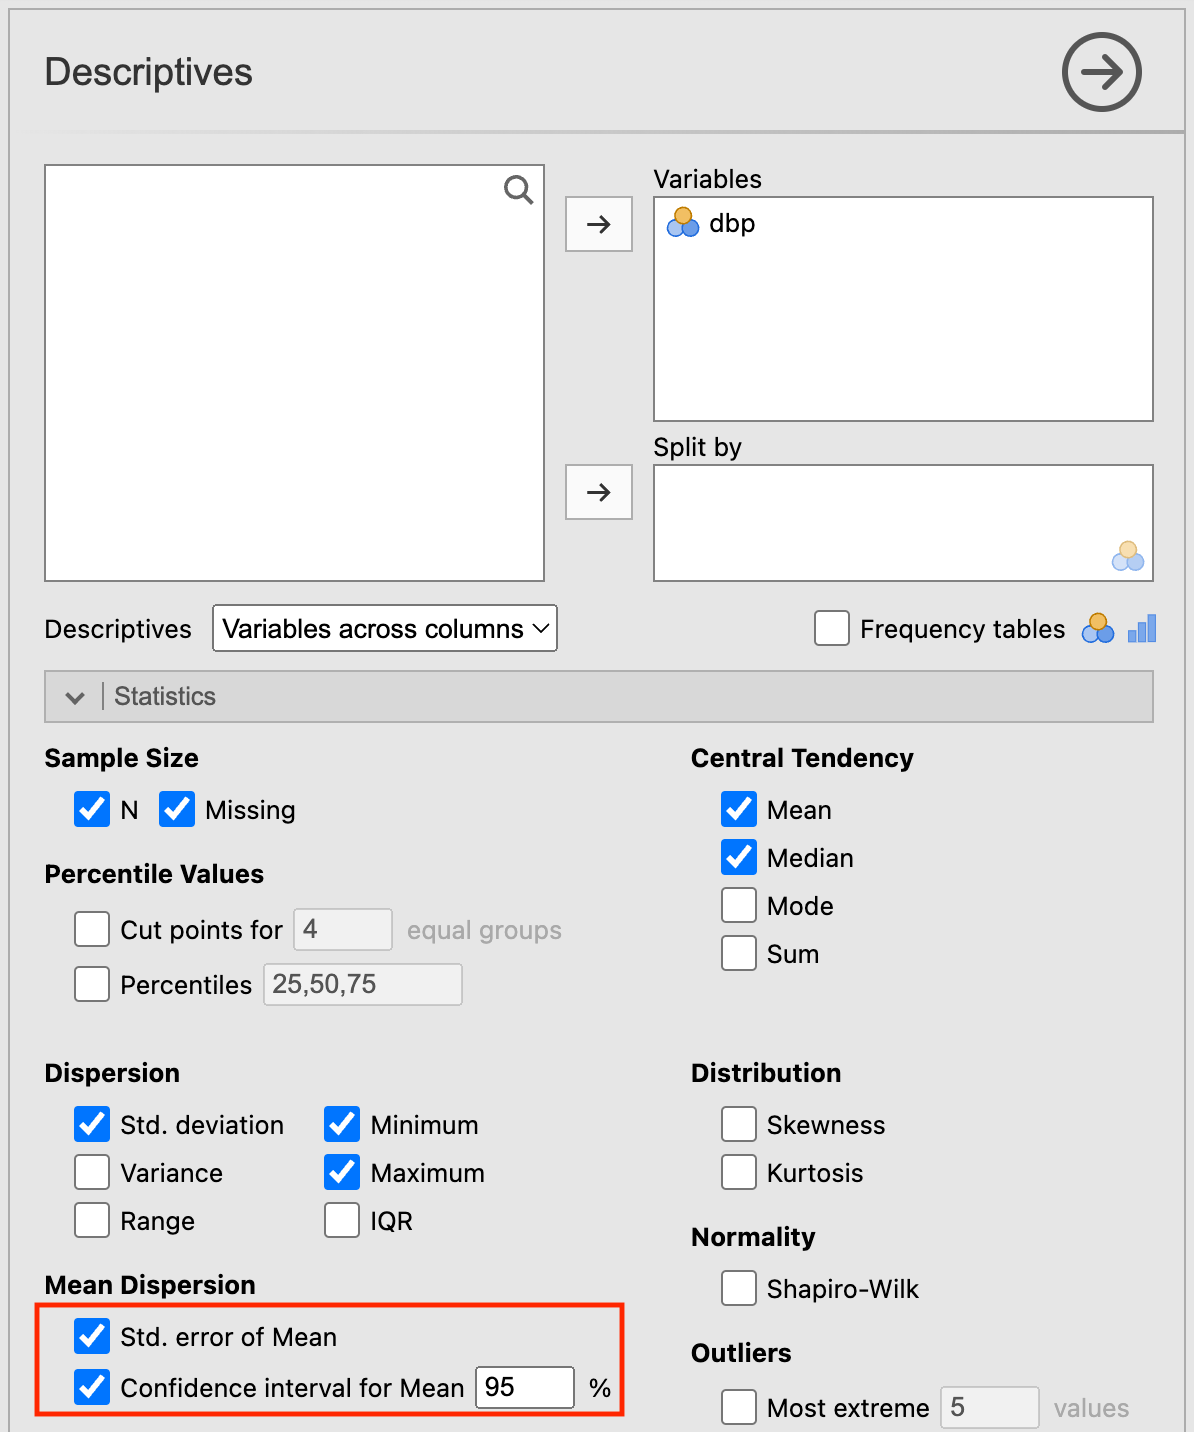
\includegraphics[keepaspectratio]{img/mod03/jamovi/mod3-desc-ci1.png}}

The descriptives output appears:

\pandocbounded{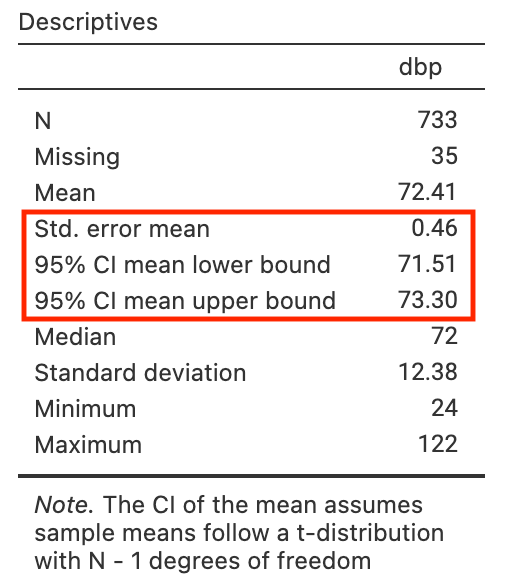
\includegraphics[keepaspectratio]{img/mod03/jamovi/mod3-desc-ci2.png}}

\section{Calculating a 95\% confidence interval of a mean: Summarised
data}\label{sec-cimean-jamovi-summ}

For Worked Example 3.2 where we are given the sample mean, sample
standard deviation and sample size, we need to install a new Jamovi
module, called \textbf{esci}. To install a new module, click the large
\textbf{+ Modules} button on the right-hand side of the Jamovi window,
and then choose \textbf{jamovi library}:

\pandocbounded{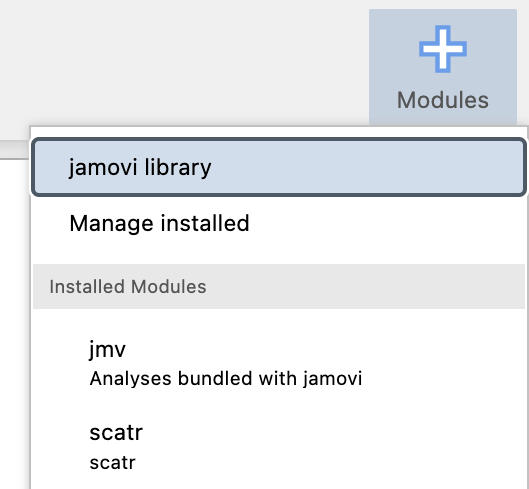
\includegraphics[keepaspectratio]{img/mod03/jamovi/mod3-inst-module1.png}}

To install a new module:

\begin{enumerate}
\def\labelenumi{\arabic{enumi}.}
\tightlist
\item
  Ensure that the middle tab, \textbf{Available} is selected;
\item
  Type \textbf{esci} in the search bar. The \textbf{esci} module will
  appear;
\item
  Click \textbf{INSTALL} to install the module
\item
  Click the up-arrow to exit from the Install Module window
\end{enumerate}

\pandocbounded{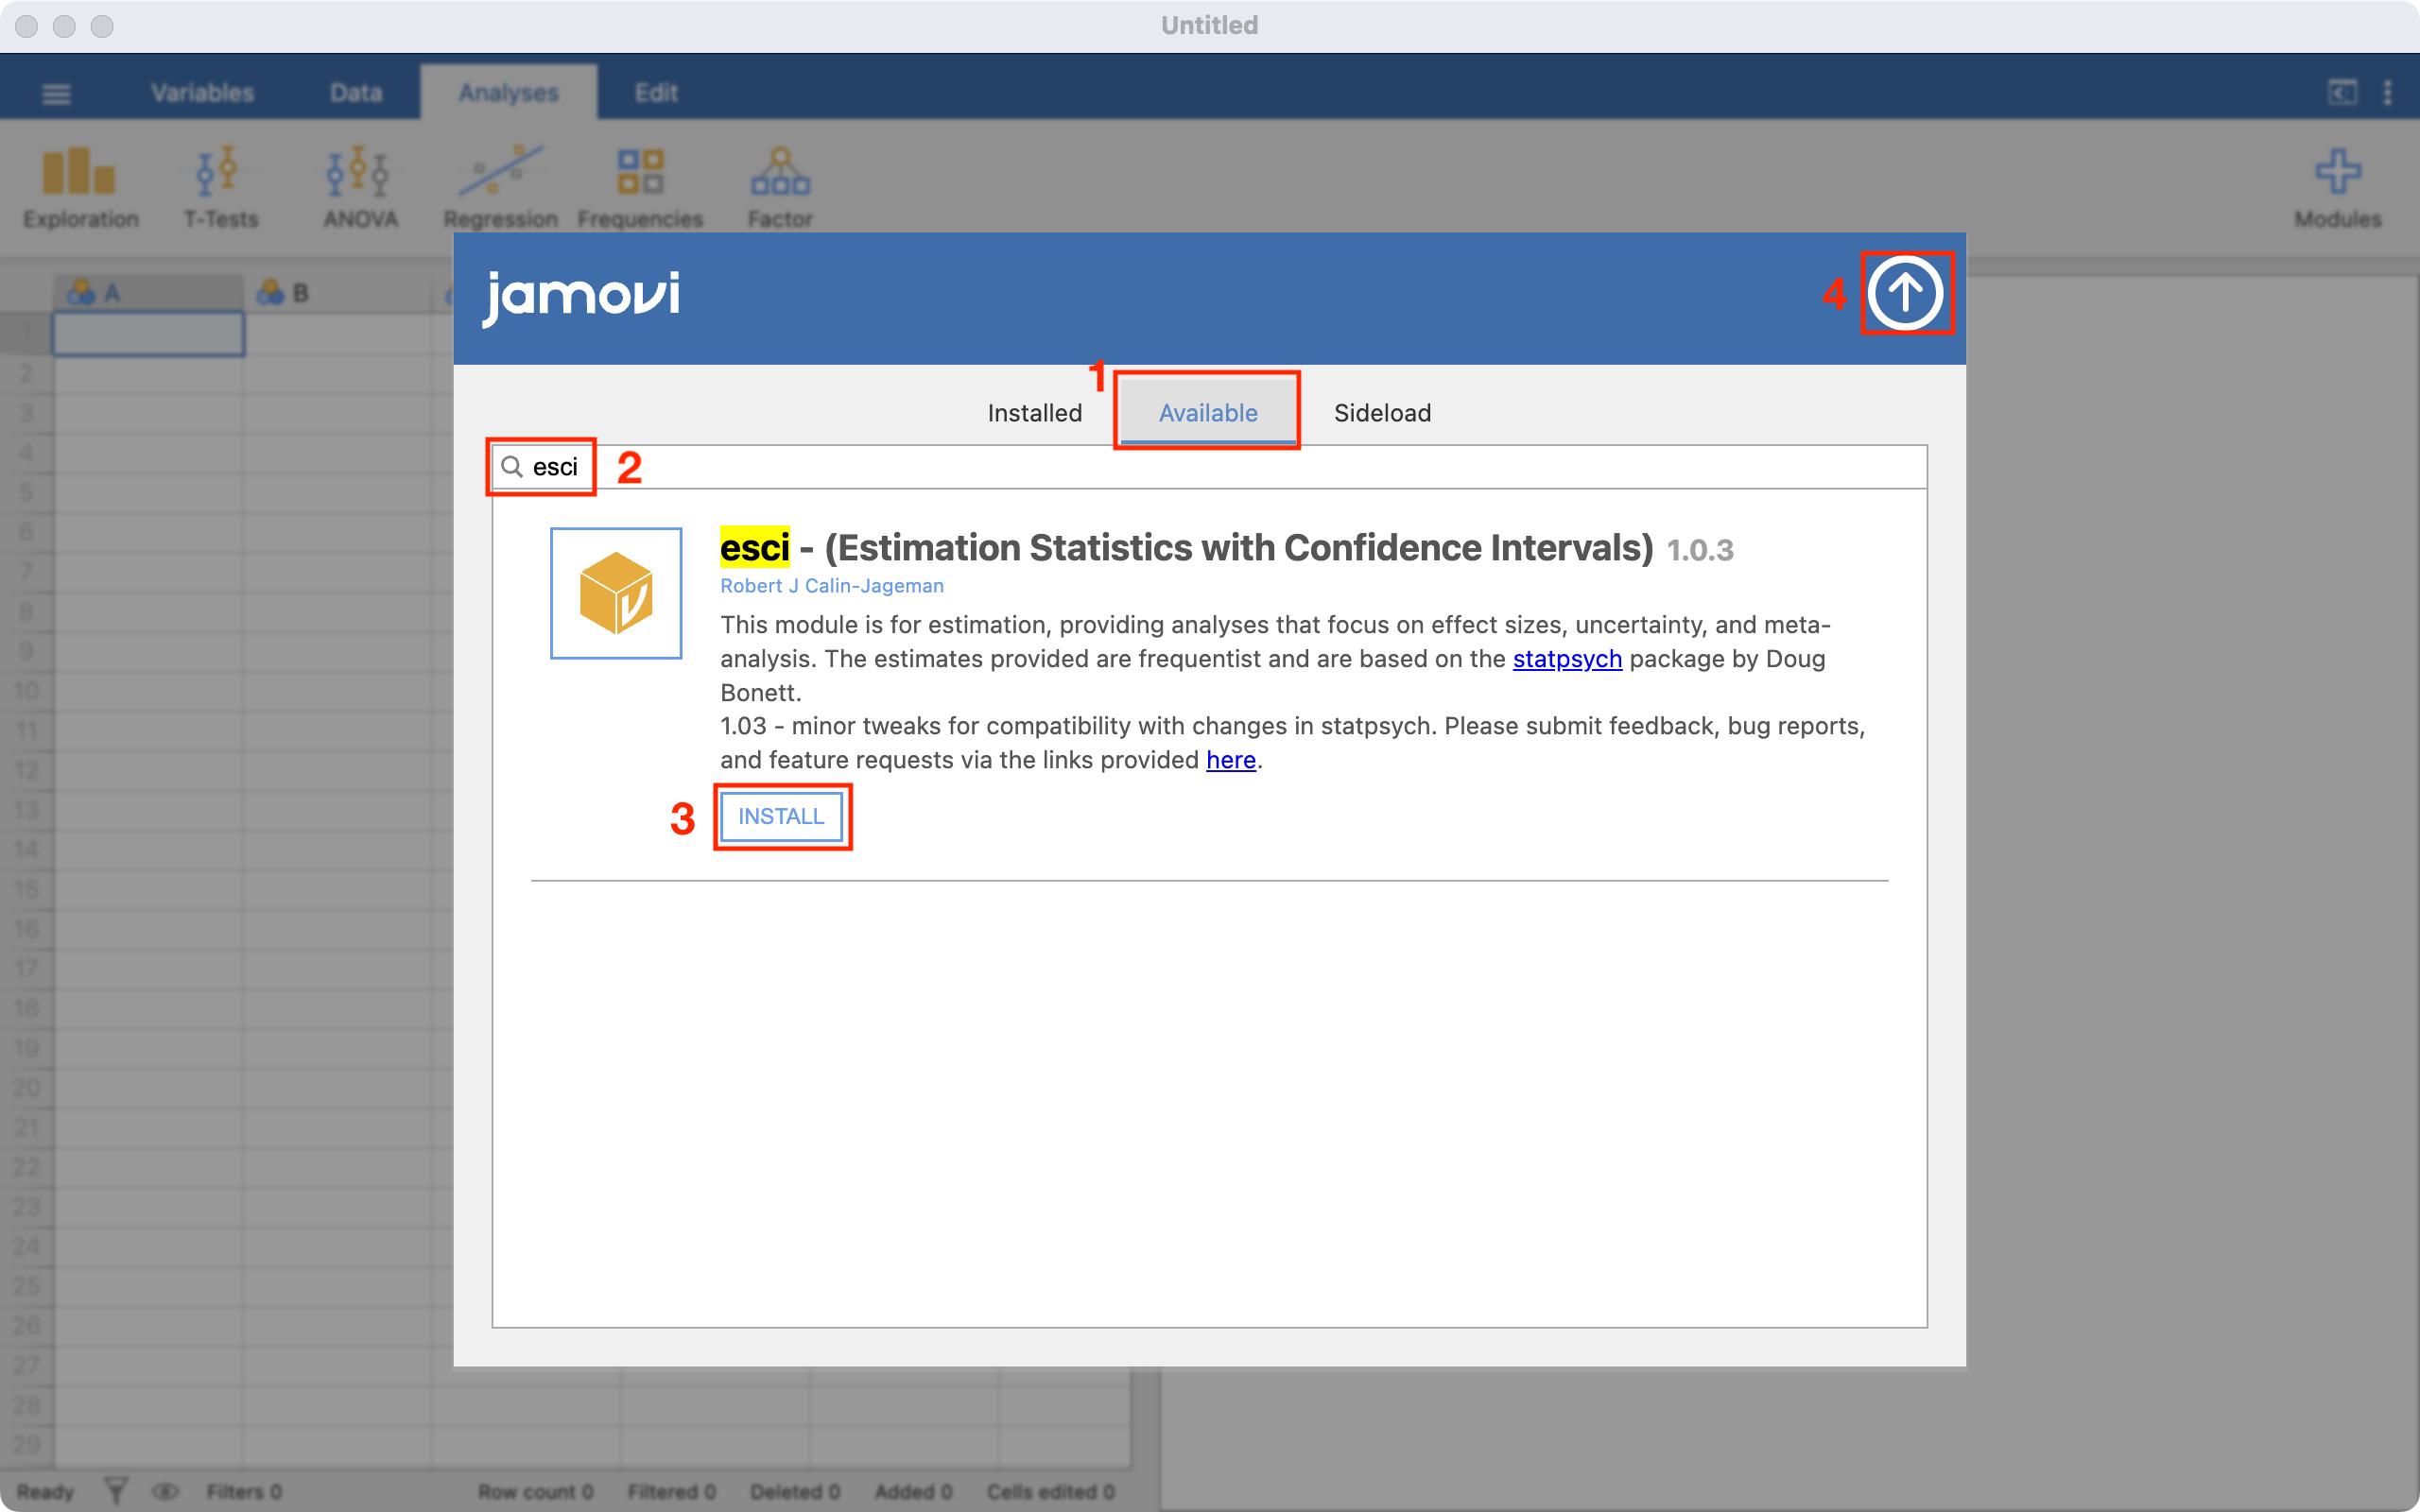
\includegraphics[keepaspectratio]{img/mod03/jamovi/mod3-inst-module2.png}}

To calculate the 95\% confidence interval, choose \textbf{esci
\textgreater{} Means and Medians \textgreater{} Single Group}. Select
the \textbf{Analyze summary data} tab, and enter the known information:
here \texttt{128.4} as the \textbf{Mean}, \texttt{19.56} as the
\textbf{Standard deviation} and \texttt{242} as the \textbf{Sample
size}. Choose \textbf{Extra details} to obtain the Standard Error of the
mean:

\pandocbounded{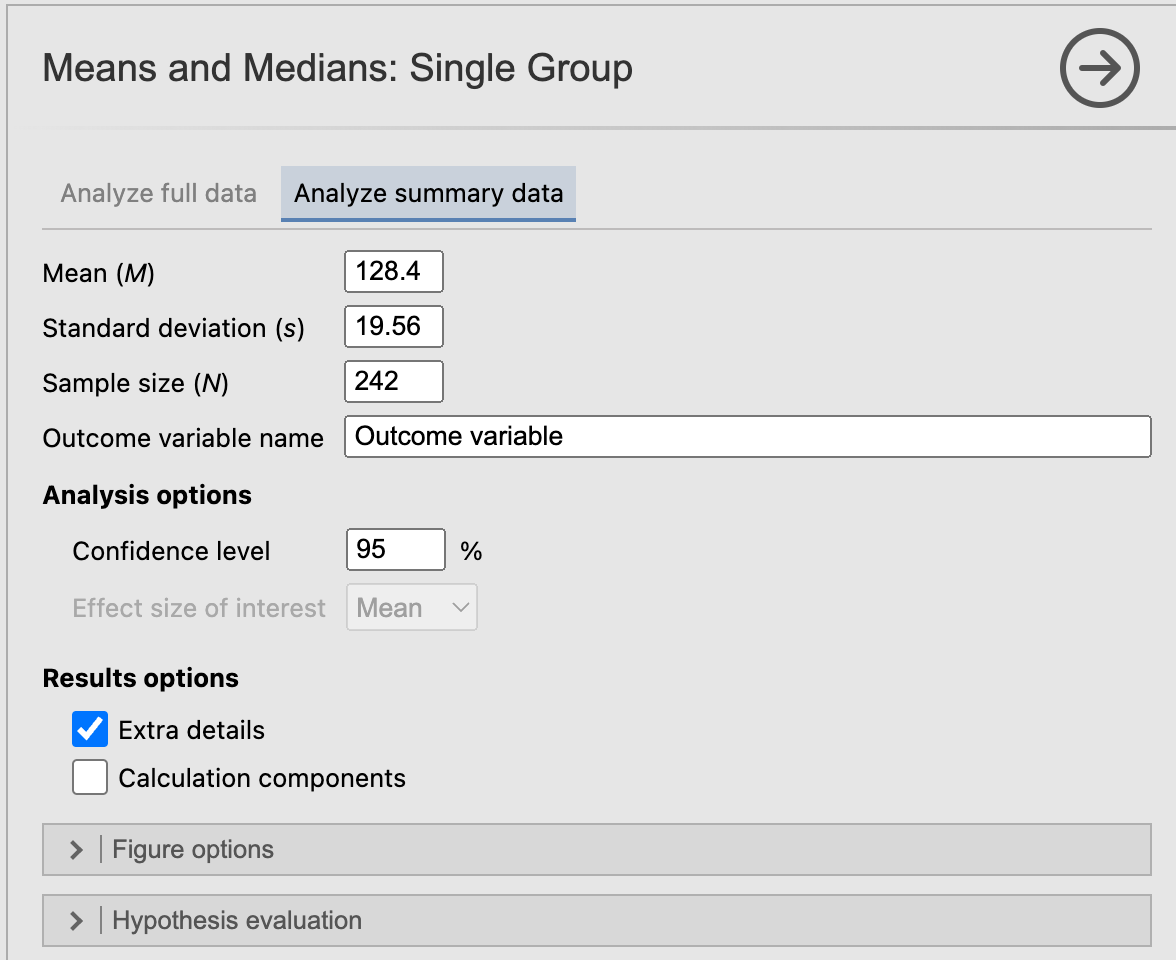
\includegraphics[keepaspectratio]{img/mod03/jamovi/mod3-cii1.png}}

The 95\% confidence interval is listed as the lower limit (LL) and the
upper limit (UL):

\pandocbounded{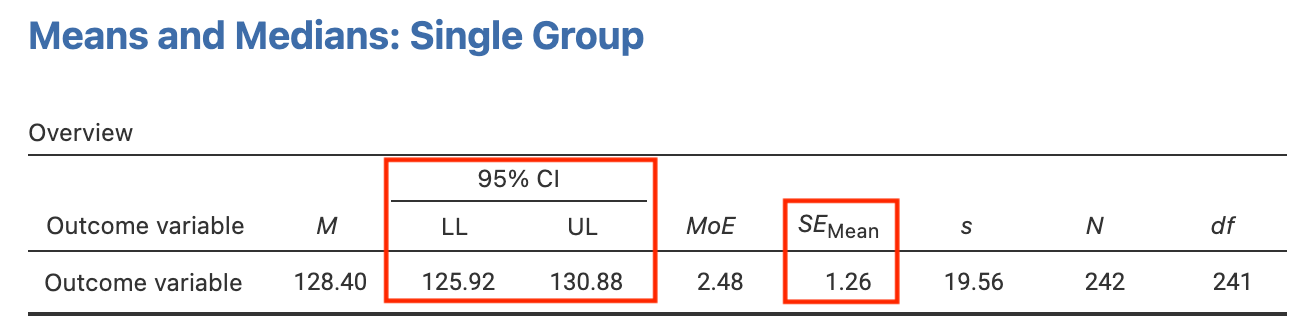
\includegraphics[keepaspectratio]{img/mod03/jamovi/mod3-cii2.png}}

\newpage{}

\bookmarksetup{startatroot}

\chapter*{R notes}\label{r-notes-1}
\addcontentsline{toc}{chapter}{R notes}

\markboth{R notes}{R notes}

\section{Importing Excel data into R}\label{importing-excel-data-into-r}

A common type of file that data are stored in is a Microsoft Excel file
(.xls or .xlsx). In this demonstration, we will import a selection of
records from a large health survey, stored in the file
\texttt{mod03\_health\_survey.xlsx}.

The health survey data contains 1140 records, comprising:

\begin{itemize}
\tightlist
\item
  sex: 1 = respondent identifies as male; 2 = respondent identifies as
  female
\item
  height: height in meters
\item
  weight: weight in kilograms
\end{itemize}

To import data from Microsoft Excel, we can use the
\texttt{read\_excel()} function in the \texttt{readxl} package.

\begin{Shaded}
\begin{Highlighting}[]
\CommentTok{\# Install the package if required}
\CommentTok{\# install.packages("readxl")}
\FunctionTok{library}\NormalTok{(readxl)}

\NormalTok{survey }\OtherTok{\textless{}{-}} \FunctionTok{read\_excel}\NormalTok{(}\StringTok{"data/examples/mod03\_health\_survey.xlsx"}\NormalTok{)}
\FunctionTok{summary}\NormalTok{(survey)}
\end{Highlighting}
\end{Shaded}

\begin{verbatim}
      sex           height          weight      
 Min.   :1.00   Min.   :1.220   Min.   : 22.70  
 1st Qu.:1.00   1st Qu.:1.630   1st Qu.: 68.00  
 Median :2.00   Median :1.700   Median : 79.40  
 Mean   :1.55   Mean   :1.698   Mean   : 81.19  
 3rd Qu.:2.00   3rd Qu.:1.780   3rd Qu.: 90.70  
 Max.   :2.00   Max.   :2.010   Max.   :213.20  
\end{verbatim}

We can see that sex has been entered as a numeric variable. We should
transform it into a factor so that we can assign labels to each
category:

\begin{Shaded}
\begin{Highlighting}[]
\NormalTok{survey}\SpecialCharTok{$}\NormalTok{sex }\OtherTok{\textless{}{-}} \FunctionTok{factor}\NormalTok{(survey}\SpecialCharTok{$}\NormalTok{sex, }\AttributeTok{levels=}\FunctionTok{c}\NormalTok{(}\DecValTok{1}\NormalTok{,}\DecValTok{2}\NormalTok{), }\AttributeTok{labels=}\FunctionTok{c}\NormalTok{(}\StringTok{"Male"}\NormalTok{, }\StringTok{"Female"}\NormalTok{))}

\FunctionTok{summary}\NormalTok{(survey}\SpecialCharTok{$}\NormalTok{sex)}
\end{Highlighting}
\end{Shaded}

\begin{verbatim}
  Male Female 
   513    627 
\end{verbatim}

We also note that height looks like it has been entered as meters, and
weight as kilograms.

\section{Generating new variables}\label{generating-new-variables-1}

Our health survey data contains information on height and weight. We
often summarise body size using BMI: body mass index which is calculated
as: \(\frac{\text{weight (kg)}}{(\text{height (m)})^2}\)

We can create a new column in our data frame in many ways, such as using
the following approach:

\texttt{dataframe\$new\_column\ \textless{}-\ \textless{}formula\textgreater{}}

For example:

\begin{Shaded}
\begin{Highlighting}[]
\NormalTok{survey}\SpecialCharTok{$}\NormalTok{bmi }\OtherTok{\textless{}{-}}\NormalTok{ survey}\SpecialCharTok{$}\NormalTok{weight }\SpecialCharTok{/}\NormalTok{ (survey}\SpecialCharTok{$}\NormalTok{height}\SpecialCharTok{\^{}}\DecValTok{2}\NormalTok{)}
\end{Highlighting}
\end{Shaded}

We should check the construction of the new variable by examining some
records. The \texttt{head()} and \texttt{tail()} functions list the
first and last 6 records in any dataset.

\begin{Shaded}
\begin{Highlighting}[]
\FunctionTok{head}\NormalTok{(survey)}
\end{Highlighting}
\end{Shaded}

\begin{verbatim}
# A tibble: 6 x 4
  sex    height weight   bmi
  <fct>   <dbl>  <dbl> <dbl>
1 Male     1.63   81.7  30.8
2 Male     1.63   68    25.6
3 Male     1.85   97.1  28.4
4 Male     1.78   89.8  28.3
5 Male     1.73   70.3  23.5
6 Female   1.57   85.7  34.8
\end{verbatim}

\begin{Shaded}
\begin{Highlighting}[]
\FunctionTok{tail}\NormalTok{(survey)}
\end{Highlighting}
\end{Shaded}

\begin{verbatim}
# A tibble: 6 x 4
  sex    height weight   bmi
  <fct>   <dbl>  <dbl> <dbl>
1 Female   1.65   95.7  35.2
2 Male     1.8    79.4  24.5
3 Female   1.73   83    27.7
4 Female   1.57   61.2  24.8
5 Male     1.7    73    25.3
6 Female   1.55   91.2  38.0
\end{verbatim}

We should also check the construction of any new variable buy examining
a density plot and/or a boxplot:

\begin{Shaded}
\begin{Highlighting}[]
\FunctionTok{library}\NormalTok{(ggplot2)}

\FunctionTok{ggplot}\NormalTok{(}\AttributeTok{data=}\NormalTok{survey, }\AttributeTok{mapping=}\FunctionTok{aes}\NormalTok{(}\AttributeTok{x=}\NormalTok{bmi)) }\SpecialCharTok{+}
  \FunctionTok{geom\_density}\NormalTok{() }\SpecialCharTok{+}
  \FunctionTok{theme\_classic}\NormalTok{() }\SpecialCharTok{+}
  \FunctionTok{labs}\NormalTok{(}\AttributeTok{x=}\StringTok{"BMI (kg/m2)"}\NormalTok{)}


\FunctionTok{ggplot}\NormalTok{(}\AttributeTok{data=}\NormalTok{survey, }\AttributeTok{mapping=}\FunctionTok{aes}\NormalTok{(}\AttributeTok{y=}\NormalTok{bmi)) }\SpecialCharTok{+}
  \FunctionTok{geom\_boxplot}\NormalTok{() }\SpecialCharTok{+}
  \FunctionTok{theme\_classic}\NormalTok{() }\SpecialCharTok{+}
  \FunctionTok{labs}\NormalTok{(}\AttributeTok{y=}\StringTok{"BMI (kg/m2)"}\NormalTok{) }\SpecialCharTok{+}
  \FunctionTok{theme}\NormalTok{(}
    \AttributeTok{axis.title.x =} \FunctionTok{element\_blank}\NormalTok{(),}
    \AttributeTok{axis.text.x =} \FunctionTok{element\_blank}\NormalTok{(),}
    \AttributeTok{axis.ticks.x =} \FunctionTok{element\_blank}\NormalTok{())}
\end{Highlighting}
\end{Shaded}

\pandocbounded{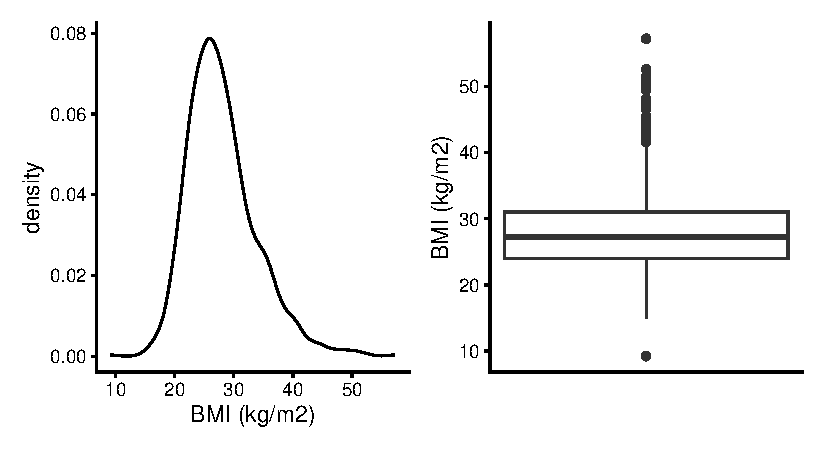
\includegraphics[keepaspectratio]{03-precision_files/figure-pdf/unnamed-chunk-7-1.pdf}}

In the general population, BMI ranges between about 15 to 30. It appears
that BMI has been correctly generated in this example. We should
investigate the very low and some of the very high values of BMI, but
this will be left for another time.

\section{\texorpdfstring{Introducing the \texttt{dplyr}
package}{Introducing the dplyr package}}\label{introducing-the-dplyr-package}

\texttt{dplyr} is a package that provides a set of functions to
manipulate data. We have previously created new columns of data, or
changed existing columns using \texttt{\textless{}-}. In \texttt{dplyr},
we can use the \texttt{mutate()} function to create new variables or to
change existing variables. The advantage of \texttt{mutate()} is that we
can create multiple new variables in the one function, using code that
is easy to read.

For example, in this module we have used \texttt{\textless{}-} to:

\begin{enumerate}
\def\labelenumi{\arabic{enumi}.}
\tightlist
\item
  define \texttt{sex} as a \textbf{factor}, and
\item
  create BMI.
\end{enumerate}

We could do these manipulations using \texttt{mutate()} as:

\begin{Shaded}
\begin{Highlighting}[]
\FunctionTok{library}\NormalTok{(dplyr)}

\NormalTok{survey }\OtherTok{\textless{}{-}} \FunctionTok{mutate}\NormalTok{(survey, }\AttributeTok{sex =} \FunctionTok{factor}\NormalTok{(sex, }\AttributeTok{levels=}\FunctionTok{c}\NormalTok{(}\DecValTok{1}\NormalTok{,}\DecValTok{2}\NormalTok{), }\AttributeTok{labels=}\FunctionTok{c}\NormalTok{(}\StringTok{"Male"}\NormalTok{, }\StringTok{"Female"}\NormalTok{)),}
                         \AttributeTok{bmi =}\NormalTok{ weight }\SpecialCharTok{/}\NormalTok{ height}\SpecialCharTok{\^{}}\DecValTok{2}\NormalTok{)}
\end{Highlighting}
\end{Shaded}

Note that the results of \texttt{\textless{}-} and \texttt{mutate()} are
identical. Some authors, however, see the \texttt{mutate()} approach
easier to read.

\section{Summarising data by another
variable}\label{summarising-data-by-another-variable-1}

We will often want to calculate the same summary statistics by another
variable. For example, we might want to calculate summary statistics for
BMI for males and females separately. We can do this in in the
\texttt{descriptives} function by defining sex as a \texttt{splitBy}
variable:

\begin{Shaded}
\begin{Highlighting}[]
\FunctionTok{library}\NormalTok{(jmv)}
\FunctionTok{descriptives}\NormalTok{(}\AttributeTok{data=}\NormalTok{survey, }\AttributeTok{vars=}\NormalTok{bmi, }\AttributeTok{splitBy =}\NormalTok{ sex)}
\end{Highlighting}
\end{Shaded}

\begin{verbatim}

 DESCRIPTIVES

 Descriptives                                 
 ──────────────────────────────────────────── 
                         sex       bmi        
 ──────────────────────────────────────────── 
   N                     Male           513   
                         Female         627   
   Missing               Male             0   
                         Female           0   
   Mean                  Male      28.29561   
                         Female    27.81434   
   Median                Male      27.39592   
                         Female    26.66667   
   Standard deviation    Male      5.204975   
                         Female    6.380523   
   Minimum               Male      16.47519   
                         Female    9.209299   
   Maximum               Male      57.23644   
                         Female    52.59516   
 ──────────────────────────────────────────── 
\end{verbatim}

\section{\texorpdfstring{Using \texttt{ggplot2} to plot density plots by
another
variable}{Using ggplot2 to plot density plots by another variable}}\label{using-ggplot2-to-plot-density-plots-by-another-variable}

We can define a grouping variable as a \texttt{facet\_wrap} to create a
grid of graphs separately for each value of the grouping variable. For
example, to create a density plot for each sex, we would use
\texttt{facet\_wrap(vars(sex))} as follows:

\begin{Shaded}
\begin{Highlighting}[]
\FunctionTok{ggplot}\NormalTok{(}\AttributeTok{data=}\NormalTok{survey, }\AttributeTok{mapping=}\FunctionTok{aes}\NormalTok{(}\AttributeTok{x=}\NormalTok{bmi)) }\SpecialCharTok{+}
  \FunctionTok{geom\_density}\NormalTok{() }\SpecialCharTok{+}
  \FunctionTok{facet\_wrap}\NormalTok{(}\FunctionTok{vars}\NormalTok{(sex)) }\SpecialCharTok{+}
  \FunctionTok{theme\_classic}\NormalTok{() }\SpecialCharTok{+}
  \FunctionTok{labs}\NormalTok{(}\AttributeTok{x=}\StringTok{"BMI (kg/m2)"}\NormalTok{)}
\end{Highlighting}
\end{Shaded}

\pandocbounded{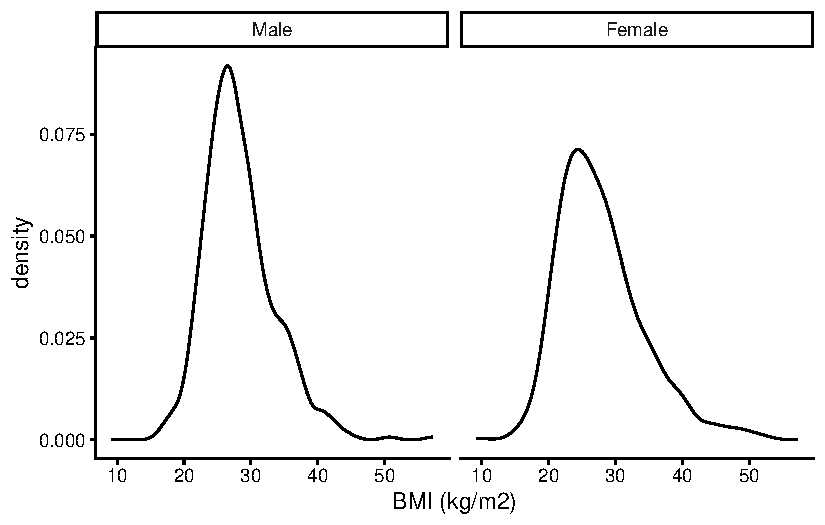
\includegraphics[keepaspectratio]{03-precision_files/figure-pdf/unnamed-chunk-10-1.pdf}}

\section{\texorpdfstring{Using \texttt{ggplot2} to plot boxplots plots
by another
variable}{Using ggplot2 to plot boxplots plots by another variable}}\label{using-ggplot2-to-plot-boxplots-plots-by-another-variable}

As for density plots, we can use a \texttt{facet\_wrap} for boxplots.
Alternatively (and possibly easier), we can define \texttt{sex} as an
\texttt{x} variable in our \texttt{mapping} statement:

\begin{Shaded}
\begin{Highlighting}[]
\FunctionTok{ggplot}\NormalTok{(}\AttributeTok{data=}\NormalTok{survey, }\AttributeTok{mapping=}\FunctionTok{aes}\NormalTok{(}\AttributeTok{y=}\NormalTok{bmi, }\AttributeTok{x=}\NormalTok{sex)) }\SpecialCharTok{+}
  \FunctionTok{geom\_boxplot}\NormalTok{() }\SpecialCharTok{+}
  \FunctionTok{theme\_classic}\NormalTok{() }\SpecialCharTok{+}
  \FunctionTok{labs}\NormalTok{(}\AttributeTok{y=}\StringTok{"BMI (kg/m2)"}\NormalTok{)}
\end{Highlighting}
\end{Shaded}

\pandocbounded{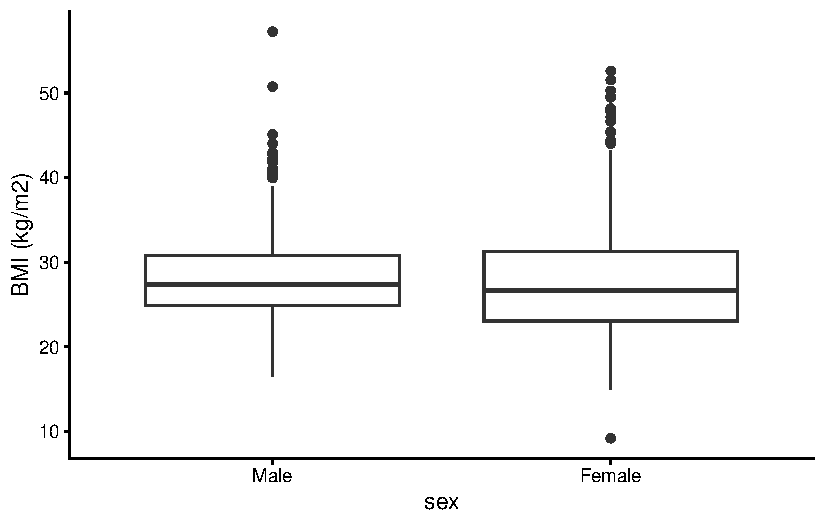
\includegraphics[keepaspectratio]{03-precision_files/figure-pdf/unnamed-chunk-11-1.pdf}}

\section{Summarising a single column of
data}\label{summarising-a-single-column-of-data}

In Module 1, we started with a very simple analysis: reading in six
ages, and them using \texttt{summary()} to calculate descriptive
statistics. We then went on to use the \texttt{decriptives()} function
in the \texttt{jmv} package as more flexible way of calculating
descriptive statistics. Let's revisit this analysis:

\begin{Shaded}
\begin{Highlighting}[]
\CommentTok{\# Author: Timothy Dobbins}
\CommentTok{\# Date: 5 April 2022}
\CommentTok{\# Purpose: My first R script}
\FunctionTok{library}\NormalTok{(jmv)}

\NormalTok{age }\OtherTok{\textless{}{-}} \FunctionTok{c}\NormalTok{(}\DecValTok{20}\NormalTok{, }\DecValTok{25}\NormalTok{, }\DecValTok{23}\NormalTok{, }\DecValTok{29}\NormalTok{, }\DecValTok{21}\NormalTok{, }\DecValTok{27}\NormalTok{)}

\CommentTok{\# Use "summary" to obtain descriptive statistics}
\FunctionTok{summary}\NormalTok{(age)}
\end{Highlighting}
\end{Shaded}

\begin{verbatim}
   Min. 1st Qu.  Median    Mean 3rd Qu.    Max. 
  20.00   21.50   24.00   24.17   26.50   29.00 
\end{verbatim}

\begin{Shaded}
\begin{Highlighting}[]
\CommentTok{\# Use the "descriptives" function from jmv to obtain descriptive statistics}
\FunctionTok{descriptives}\NormalTok{(age)}
\end{Highlighting}
\end{Shaded}

\begin{verbatim}
Error:
! Argument 'data' must be a data frame
\end{verbatim}

The \texttt{summary()} function has worked correctly, but the
\texttt{descriptives()} function has given an error:
\texttt{Error:\ Argument\ \textquotesingle{}data\textquotesingle{}\ must\ be\ a\ data\ frame}.
What on earth is going on here?

The error gives us a clue here - the \texttt{descriptives()} function
requires a data frame for analysis. We have provided the object
\texttt{age}: a \textbf{vector}. As we saw in
Section~\ref{sec-data-structures}, a vector is a single column of data,
while a data frame is a collection of columns.

In order to summarise a vector using the \texttt{descriptives()}
function, we must first convert the vector into a data frame using
\texttt{as.data.frame()}. For example:

\begin{Shaded}
\begin{Highlighting}[]
\CommentTok{\# Author: Timothy Dobbins}
\CommentTok{\# Date: 5 April 2024}
\CommentTok{\# Purpose: My first R script}
\FunctionTok{library}\NormalTok{(jmv)}

\NormalTok{age }\OtherTok{\textless{}{-}} \FunctionTok{c}\NormalTok{(}\DecValTok{20}\NormalTok{, }\DecValTok{25}\NormalTok{, }\DecValTok{23}\NormalTok{, }\DecValTok{29}\NormalTok{, }\DecValTok{21}\NormalTok{, }\DecValTok{27}\NormalTok{)}

\CommentTok{\# Use "summary" to obtain descriptive statistics}
\FunctionTok{summary}\NormalTok{(age)}
\end{Highlighting}
\end{Shaded}

\begin{verbatim}
   Min. 1st Qu.  Median    Mean 3rd Qu.    Max. 
  20.00   21.50   24.00   24.17   26.50   29.00 
\end{verbatim}

\begin{Shaded}
\begin{Highlighting}[]
\CommentTok{\# Create a new data frame from the vector age:}

\NormalTok{age\_df }\OtherTok{\textless{}{-}} \FunctionTok{as.data.frame}\NormalTok{(age)}

\CommentTok{\# Use "descriptives" to obtain descriptive statistics for age\_df}
\FunctionTok{descriptives}\NormalTok{(age\_df)}
\end{Highlighting}
\end{Shaded}

\begin{verbatim}

 DESCRIPTIVES

 Descriptives                       
 ────────────────────────────────── 
                         age        
 ────────────────────────────────── 
   N                            6   
   Missing                      0   
   Mean                  24.16667   
   Median                24.00000   
   Standard deviation    3.488075   
   Minimum               20.00000   
   Maximum               29.00000   
 ────────────────────────────────── 
\end{verbatim}

\section{Computing probabilities from a Normal
distribution}\label{sec-normal-r}

The Normal Distribution Applet posted at
\url{https://mabognar.github.io/apps/normal.html}, provides a simple and
intuitive way to compute probabilities from a binomial distribution.
Refer to the jamovi instructions for details.

We can use the \texttt{pnorm} function to calculate probabilities from a
Normal distribution:

\begin{itemize}
\tightlist
\item
  \texttt{pnorm(q,\ mean,\ sd)} calculates the probability of observing
  a value of \texttt{q} or less, from a Normal distribution with a mean
  of \texttt{mean} and a standard deviation of \texttt{sd}. Note that if
  \texttt{mean} and \texttt{sd} are not entered, they are assumed to be
  0 and 1 respectively (i.e.~a standard normal distribution.)
\item
  \texttt{pnorm(q,\ mean,\ sd,\ lower.tail=FALSE)} calculates the
  probability of observing a value of more than \texttt{q}, from a
  Normal distribution with a mean of \texttt{mean} and a standard
  deviation of \texttt{sd}.
\end{itemize}

To obtain the probability of obtaining 0.5 or greater from a standard
normal distribution:

\begin{Shaded}
\begin{Highlighting}[]
\FunctionTok{pnorm}\NormalTok{(}\FloatTok{0.5}\NormalTok{, }\AttributeTok{lower.tail =} \ConstantTok{FALSE}\NormalTok{)}
\end{Highlighting}
\end{Shaded}

\begin{verbatim}
[1] 0.3085375
\end{verbatim}

To calculate the worked example: Assume that the mean diastolic blood
pressure for men is 77.9 mmHg, with a standard deviation of 11. What is
the probability that a man selected at random will have high blood
pressure (i.e.~diastolic blood pressure greater than or equal to 90)?

\begin{Shaded}
\begin{Highlighting}[]
\FunctionTok{pnorm}\NormalTok{(}\DecValTok{90}\NormalTok{, }\AttributeTok{mean =} \FloatTok{77.9}\NormalTok{, }\AttributeTok{sd =} \DecValTok{11}\NormalTok{, }\AttributeTok{lower.tail =} \ConstantTok{FALSE}\NormalTok{)}
\end{Highlighting}
\end{Shaded}

\begin{verbatim}
[1] 0.1356661
\end{verbatim}

\section{Calculating a 95\% confidence interval of a mean: individual
data}\label{sec-cimean-r-ind}

To demonstrate the computation of the 95\% confidence interval of a
mean, we can use the data from \texttt{mod03\_blood\_pressure.csv}:

\begin{Shaded}
\begin{Highlighting}[]
\NormalTok{pima }\OtherTok{\textless{}{-}} \FunctionTok{read.csv}\NormalTok{(}\StringTok{"data/examples/mod03\_blood\_pressure.csv"}\NormalTok{)}
\end{Highlighting}
\end{Shaded}

We can examine the data set using the \texttt{summary} command:

\begin{Shaded}
\begin{Highlighting}[]
\FunctionTok{summary}\NormalTok{(pima)}
\end{Highlighting}
\end{Shaded}

\begin{verbatim}
      dbp        
 Min.   : 24.00  
 1st Qu.: 64.00  
 Median : 72.00  
 Mean   : 72.41  
 3rd Qu.: 80.00  
 Max.   :122.00  
\end{verbatim}

The mean and its 95\% confidence interval can be obtained many ways in
R. We will use the \texttt{descriptives()} function within the
\texttt{jmv} package to calculate the standard error of the mean, and a
confidence interval, by including \texttt{se\ =\ TRUE} and
\texttt{ci\ =\ TRUE}:

\begin{Shaded}
\begin{Highlighting}[]
\FunctionTok{library}\NormalTok{(jmv)}
\FunctionTok{descriptives}\NormalTok{(}\AttributeTok{data=}\NormalTok{pima, }\AttributeTok{vars=}\NormalTok{dbp, }\AttributeTok{se=}\ConstantTok{TRUE}\NormalTok{, }\AttributeTok{ci=}\ConstantTok{TRUE}\NormalTok{)}
\end{Highlighting}
\end{Shaded}

\begin{verbatim}

 DESCRIPTIVES

 Descriptives                             
 ──────────────────────────────────────── 
                              dbp         
 ──────────────────────────────────────── 
   N                                733   
   Missing                            0   
   Mean                        72.40518   
   Std. error mean            0.4573454   
   95% CI mean lower bound     71.50732   
   95% CI mean upper bound     73.30305   
   Median                            72   
   Standard deviation          12.38216   
   Minimum                           24   
   Maximum                          122   
 ──────────────────────────────────────── 
   Note. The CI of the mean assumes
   sample means follow a
   t-distribution with N - 1 degrees
   of freedom
\end{verbatim}

\section{Calculating a 95\% confidence interval of a mean: summarised
data}\label{sec-cimean-r-summ}

For Worked Example 3.2 where we are given the sample mean, sample
standard deviation and sample size. R does not have a built-in function
to calculate a confidence interval from summarised data, but we can
write our own.

\textbf{Note: writing your own functions is beyond the scope of this
course. You should copy and paste the code provided to do this.}

\begin{Shaded}
\begin{Highlighting}[]
\DocumentationTok{\#\#\# Copy this section}
\NormalTok{ci\_mean }\OtherTok{\textless{}{-}} \ControlFlowTok{function}\NormalTok{(n, mean, sd, }\AttributeTok{width=}\FloatTok{0.95}\NormalTok{, }\AttributeTok{digits=}\DecValTok{3}\NormalTok{)\{}
\NormalTok{  lcl }\OtherTok{\textless{}{-}}\NormalTok{ mean }\SpecialCharTok{{-}} \FunctionTok{qt}\NormalTok{(}\AttributeTok{p=}\NormalTok{(}\DecValTok{1} \SpecialCharTok{{-}}\NormalTok{ (}\DecValTok{1}\SpecialCharTok{{-}}\NormalTok{width)}\SpecialCharTok{/}\DecValTok{2}\NormalTok{), }\AttributeTok{df=}\NormalTok{n}\DecValTok{{-}1}\NormalTok{) }\SpecialCharTok{*}\NormalTok{ sd}\SpecialCharTok{/}\FunctionTok{sqrt}\NormalTok{(n)}
\NormalTok{  ucl }\OtherTok{\textless{}{-}}\NormalTok{ mean }\SpecialCharTok{+} \FunctionTok{qt}\NormalTok{(}\AttributeTok{p=}\NormalTok{(}\DecValTok{1} \SpecialCharTok{{-}}\NormalTok{ (}\DecValTok{1}\SpecialCharTok{{-}}\NormalTok{width)}\SpecialCharTok{/}\DecValTok{2}\NormalTok{), }\AttributeTok{df=}\NormalTok{n}\DecValTok{{-}1}\NormalTok{) }\SpecialCharTok{*}\NormalTok{ sd}\SpecialCharTok{/}\FunctionTok{sqrt}\NormalTok{(n)}
  
  \FunctionTok{print}\NormalTok{(}\FunctionTok{paste0}\NormalTok{(width}\SpecialCharTok{*}\DecValTok{100}\NormalTok{, }\StringTok{"\%"}\NormalTok{, }\StringTok{" CI: "}\NormalTok{, }\FunctionTok{format}\NormalTok{(}\FunctionTok{round}\NormalTok{(lcl, }\AttributeTok{digits=}\NormalTok{digits), }\AttributeTok{nsmall =}\NormalTok{ digits),}
               \StringTok{" to "}\NormalTok{, }\FunctionTok{format}\NormalTok{(}\FunctionTok{round}\NormalTok{(ucl, }\AttributeTok{digits=}\NormalTok{digits), }\AttributeTok{nsmall =}\NormalTok{ digits) ))}

\NormalTok{\}}
\DocumentationTok{\#\#\# End of copy}

\FunctionTok{ci\_mean}\NormalTok{(}\AttributeTok{n=}\DecValTok{242}\NormalTok{, }\AttributeTok{mean=}\FloatTok{128.4}\NormalTok{, }\AttributeTok{sd=}\FloatTok{19.56}\NormalTok{, }\AttributeTok{width=}\FloatTok{0.95}\NormalTok{)}
\end{Highlighting}
\end{Shaded}

\begin{verbatim}
[1] "95% CI: 125.923 to 130.877"
\end{verbatim}

\begin{Shaded}
\begin{Highlighting}[]
\FunctionTok{ci\_mean}\NormalTok{(}\AttributeTok{n=}\DecValTok{242}\NormalTok{, }\AttributeTok{mean=}\FloatTok{128.4}\NormalTok{, }\AttributeTok{sd=}\FloatTok{19.56}\NormalTok{, }\AttributeTok{width=}\FloatTok{0.99}\NormalTok{)}
\end{Highlighting}
\end{Shaded}

\begin{verbatim}
[1] "99% CI: 125.135 to 131.665"
\end{verbatim}

\newpage{}

\bookmarksetup{startatroot}

\chapter*{Activities}\label{activities-2}
\addcontentsline{toc}{chapter}{Activities}

\markboth{Activities}{Activities}

\subsection*{Activity 3.1}\label{activity-3.1}
\addcontentsline{toc}{subsection}{Activity 3.1}

An investigator wishes to survey people living with agoraphobia (a type
of anxiety disorder). People with agoraphobia find it difficult to leave
environments they know and consider to be safe for fear of having
anxiety or a panic attack.

The investigator buys an ad on Facebook asking for volunteer
participants to complete an in-person interview. A total of 950 replies
are received of which the investigator randomly selects 50. However,
only 15 volunteers turn up for their interview.

\begin{enumerate}
\def\labelenumi{\arabic{enumi}.}
\tightlist
\item
  Which of the following statements is true?
\end{enumerate}

\begin{enumerate}
\def\labelenumi{\alph{enumi})}
\tightlist
\item
  The final 15 participants are likely to be a representative sample of
  the population available to the investigator
\item
  The final 15 participants are likely to be a representative sample of
  the population of people living with agoraphobia
\item
  The randomly selected 50 participants are likely to be a
  representative sample of people with agoraphobia who replied to the
  Facebook ad
\item
  None of the above
\end{enumerate}

\begin{enumerate}
\def\labelenumi{\arabic{enumi}.}
\setcounter{enumi}{1}
\tightlist
\item
  The basic problem confronted by the investigator is that:
\end{enumerate}

\begin{enumerate}
\def\labelenumi{\alph{enumi})}
\tightlist
\item
  The accessible population might be different from the target
  population
\item
  The sample has been chosen using an unethical method
\item
  The sample size was too small
\item
  It is difficult to obtain a sample of people living with agoraphobia
  in a scientific way
\end{enumerate}

\begin{enumerate}
\def\labelenumi{\arabic{enumi}.}
\setcounter{enumi}{2}
\tightlist
\item
  Think about how you might design a study to recruit people living with
  agoraphobia.
\end{enumerate}

\subsection*{Activity 3.2}\label{activity-3.2}
\addcontentsline{toc}{subsection}{Activity 3.2}

A dental epidemiologist wants to estimate the mean weekly consumption of
dietary sugar among preschool children in Kensington, NSW. She takes
four samples from different preschools in the area. The estimated daily
intake of total sugar consumption (in grams) are saved in
\texttt{Activity\_3.2.rds}.

\begin{enumerate}
\def\labelenumi{\alph{enumi})}
\tightlist
\item
  Obtain the sample size, the mean and standard deviation for total
  sugar consumption for each preschool. Plot the distribution of total
  sugar consumption by preschool. What do you notice about the
  variability of total sugar consumption by preschool?
\item
  Obtain the standard error of the mean total sugar consumption by
  preschool. What happens to the standard error as the sample size
  increases?
\item
  Obtain the 95\% confidence interval of the mean total sugar
  consumption by preschool, and comment.
\item
  What can you say about the precision of the sample mean as the sample
  size increases?
\item
  Interpret the 95\% confidence interval of the mean total sugar
  consumption for one preschool. What population are we making
  inferences about? Is this valid?
\end{enumerate}

\subsection*{Activity 3.3}\label{activity-3.3}
\addcontentsline{toc}{subsection}{Activity 3.3}

The dataset for this activity is the same as the one used in Activity
1.3 in Module 1: a study was conducted to investigate the general health
of undergraduate students at Australian universities. A random selection
of 218 UNSW undergradute students from UNSW were enrolled, and their
diastolic blood pressures were recorded. The file is
\texttt{Activity\_1.3.csv}.

\begin{enumerate}
\def\labelenumi{\alph{enumi})}
\tightlist
\item
  Plot diastolic blood pressure and describe the distribution.
\item
  Use jamovi or R to obtain an estimate of the mean, standard error of
  the mean and the 95\% confidence interval for the mean diastolic blood
  pressure.
\item
  Interpret the 95\% confidence interval for the mean diastolic blood
  pressure.
\end{enumerate}

\subsection*{Activity 3.4}\label{activity-3.4}
\addcontentsline{toc}{subsection}{Activity 3.4}

Using the health survey data (\texttt{Activity\_3.4.xlsx}) described in
the computing notes of this module, create a new variable, BMI, which is
equal to a person's weight (in kg) divided by their height (in metres)
squared
(i.e.~\(\text{BMI} = \frac{\text{weight (kg)}}{\text{[height (m)]}^2}\).
Categorise BMI using the categories:

\begin{itemize}
\tightlist
\item
  Underweight: BMI \textless{} 18.5
\item
  Normal weight: 18.5 \(\le\) BMI \textless{} 25
\item
  Overweight: 25 \(\le\) BMI \textless{} 30
\item
  Obese: BMI \(\ge\) 30
\end{itemize}

Note: BMI does not necessarily reflect body fat distribution or describe
the same degree of fatness in different individuals. However, at a
population level, BMI is a practical and useful measure for identifying
overweight or obesity. \footnote{https://www.aihw.gov.au/reports/overweight-obesity/overweight-and-obesity/contents/measuring-overweight-and-obesity}

Create a two-way table to display the distribution of BMI categories by
sex (sex: 1 = respondent identifies as male; 2 = respondent identifies
as female). Does there appear to be a difference in categorised BMI
between males and females?

\subsection*{Activity 3.5}\label{activity-3.5}
\addcontentsline{toc}{subsection}{Activity 3.5}

The data set of hospital stay data for 1323 hypothetical patients is
available in csv format (\texttt{Activity\_3.5.csv}). Import this
dataset into jamovi or R. There are two variables in this dataset:

\begin{itemize}
\tightlist
\item
  female: female=1; male=0
\item
  los: length of stay in days
\end{itemize}

\begin{enumerate}
\def\labelenumi{\alph{enumi})}
\tightlist
\item
  Use jamovi or R to examine the distribution of length of stay:
  overall; and separately for females and males. Comment on the
  distributions.
\item
  Use jamovi or R to calculate measures of central tendency for hospital
  stay to obtain information about the average duration of hospital
  stay. Which summary statistics should you report and why? Report the
  appropriate statistics of the spread and measure of central tendency
  chosen.
\item
  Calculate the measures of central tendency for hospital duration
  separately for males and females. What can you conclude from comparing
  these measures for males and females?
\end{enumerate}

\subsection*{Activity 3.6}\label{activity-3.6}
\addcontentsline{toc}{subsection}{Activity 3.6}

If weights of men are Normally distributed with a population mean
\(\mu\) = 87, and a population standard deviation, \(\sigma\) = 8 kg:

\begin{enumerate}
\def\labelenumi{\alph{enumi})}
\tightlist
\item
  What is the probability that a man will weigh 95 kg or more? Draw a
  Normal curve of the area represented by this probability in the
  population (i.e.~with \(\mu\) = 87 kg and \(\sigma\) = 8 kg).
\item
  What is the probability that a man will weigh more than 75 kg but less
  than 95 kg? Draw the area represented by this probability on a Normal
  curve.
\end{enumerate}

\bookmarksetup{startatroot}

\chapter{An introduction to hypothesis
testing}\label{an-introduction-to-hypothesis-testing}

\section*{Learning objectives}\label{learning-objectives-3}
\addcontentsline{toc}{section}{Learning objectives}

\markright{Learning objectives}

By the end of this module you will be able to:

\begin{itemize}
\tightlist
\item
  Formulate a research question and present it as a null and alternative
  hypothesis;
\item
  Understand the role of confidence intervals in assessing research
  questions;
\item
  Explain the general framework of hypothesis testing;
\item
  Interpret P-values as measures of evidence;
\item
  Distinguish between statistical significance and practical importance;
\item
  Perform and interpret a one-sample t-test;
\item
  Explain the concepts of one-tailed and two-tailed statistical tests,
  and determine when each is appropriate;
\item
  Report the results of hypothesis tests clearly, accurately, and in
  plain language.
\end{itemize}

\section*{Optional readings}\label{optional-readings-3}
\addcontentsline{toc}{section}{Optional readings}

\markright{Optional readings}

Kirkwood and Sterne (2001); Chapter 8.
\href{http://er1.library.unsw.edu.au/er/cgi-bin/eraccess.cgi?url=https://ebookcentral.proquest.com/lib/unsw/detail.action?docID=624728}{{[}UNSW
Library Link{]}}

Bland (2015); Sections 9.1 to 9.7; Sections 10.1 and 10.2.
\href{http://er1.library.unsw.edu.au/er/cgi-bin/eraccess.cgi?url=https://ebookcentral.proquest.com/lib/unsw/detail.action?docID=5891730}{{[}UNSW
Library Link{]}}

\section{Introduction}\label{introduction-3}

In earlier modules, we examined sampling and how summary statistics can
be used to make inferences about a population parameter. For example, we
can use the sample mean \(\bar{x}\) to make inferences about \(\mu\),
the true mean of the population from which a sample is drawn. In this
module, we introduce hypothesis testing as the basis of the statistical
tests that are important for reporting results from research and
surveillance studies, and that you will be learning in the remainder of
this course.

We use hypothesis testing to answer questions such as whether two groups
have different health outcomes or whether there is an association
between a treatment and a health outcome. For example, we may want to
know:

\begin{itemize}
\tightlist
\item
  whether a safety program has been effective in reducing injuries in a
  factory, i.e.~whether the frequency of injuries in the group who
  attended a safety program is lower than in the group who did not
  receive the safety program;
\item
  whether a new drug is more effective in reducing blood pressure than a
  conventional drug, i.e.~whether the mean blood pressure in the group
  receiving the new drug is lower than the mean blood pressure in the
  group receiving the conventional medication;
\item
  whether an environmental exposure increases the risk of a disease,
  i.e.~whether the frequency of disease is higher in the group who have
  been exposed to an environmental factor than in the non-exposed group.
\end{itemize}

We may also want to know something about a single group. For example,
whether the mean blood pressure of a sample is the same as the general
population.

These questions can be answered by setting up a null hypothesis and an
alternative hypothesis, and performing a hypothesis test (also known as
a significance test). In this module we focus on testing hypotheses
about a single population mean, using confidence intervals and the
one-sample t-test.

\subsection{Worked example}\label{worked-example-2}

In this module, we will revisit the Pima example from Module 3
(\texttt{mod03\_blood\_pressure.csv}). A sample of 733 female Pima
indigenous Americans was taken, and their diastolic blood pressure was
measured (among other measures). We saw in Module 3 that a density plot
demonstrates that the data are approximately normally distributed, and
the mean diastolic blood pressure was estimated as 72.4 mmHg with a 95\%
confidence interval from 71.5 to 73.3 mmHg.

\section{Research questions}\label{research-questions}

A research question is an open, neutral question that states what we
want to find out - often phrased using everyday language. Research
questions guide study design and data collection, and do not presuppose
an answer. Using our Pima example, a research question could be posed:

\begin{itemize}
\tightlist
\item
  Do Pima women have the same mean diastolic blood pressure as the
  general US population?
\end{itemize}

A useful way of structuring research questions in health research is the
PECO framework:

\begin{itemize}
\tightlist
\item
  Population: Who is being studied?
\item
  Exposure: What exposure, risk factor, or condition is of interest?
\item
  Comparator: What is the exposure being compared against?
\item
  Outcome: What outcome is being measured?
\end{itemize}

In the example above:

\begin{itemize}
\tightlist
\item
  Population: Pima women
\item
  Comparator: General US population
\item
  Outcome: Diastolic blood pressure
\end{itemize}

Note there as there is only one group here, there is no ``exposure''.

\section{Using confidence intervals to assess research
questions}\label{using-confidence-intervals-to-assess-research-questions}

We can use the 95\% confidence interval to \textbf{informally} assess
research questions. For example, we can use a 95\% confidence interval
for the mean to assess whether the population mean is consistent with a
hypothesised value. A confidence interval gives a range of plausible
values for the true population mean, based on the sample data, and we
can compare the confidence interval with the hypothesised value.

If a hypothesised mean lies:

\begin{itemize}
\tightlist
\item
  \emph{outside} the confidence interval, there is \emph{informal
  evidence} that the population mean differs from the hypothesised mean
\item
  \emph{inside} the confidence interval, there is \emph{no informal
  evidence} that the population mean differs from the hypothesised mean
\end{itemize}

Note that a confidence interval does not provide a quantitative measure
of evidence against a null hypothesis; it supports only an informal
comparison. Formal hypothesis testing is required to quantify the level
of evidence.

\section{Hypothesis testing}\label{hypothesis-testing}

In statistics, a hypothesis is a claim about a population parameter.
Hypothesis testing is a formal procedure used to decide between two
competing claims about a population parameter. These two claims are
known as:

\begin{itemize}
\tightlist
\item
  the \textbf{null hypothesis}
\item
  the \textbf{alternative hypothesis}
\end{itemize}

Hypothesis testing is a statistical technique that is used to quantify
the evidence against a null hypothesis.

The \textbf{null hypothesis}, written H\textsubscript{0}, represents the
hypothesis of no difference, no change, no effect. It is often described
as the \emph{boring} or \emph{skeptical} hypothesis

The \textbf{alternative hypothesis}, written H\textsubscript{A},
represents the hypothesis of a difference, change or effect.

Note that hypotheses always refer to a \textbf{population}, not a
sample.

\subsection{Example}\label{example}

In our example, our research question is: do Pima women have the same
mean diastolic blood pressure as the general US population?

To test this research question, we will need a value for the mean
diastolic blood pressure of the general US population. We will use the
results from a large-scale population survey, and state that the US
population has a mean diastolic blood pressure of 71mmHg.

Our hypotheses then, could be written as:

\begin{itemize}
\tightlist
\item
  H\textsubscript{0}: \(\mu = 71\)
\item
  H\textsubscript{A}: \(\mu \ne 71\)
\end{itemize}

where \(\mu\) is the true population mean diastolic blood pressure of
Pima women.

These hypotheses are very formal, and it may be easier to think of them
as:

\begin{itemize}
\tightlist
\item
  H\textsubscript{0}: The mean diastolic blood pressure of Pima women is
  71 mmHg.
\item
  H\textsubscript{A}: The mean diastolic blood pressure of Pima women is
  not 71 mmHg.
\end{itemize}

\section{The hypothesis testing
framework}\label{the-hypothesis-testing-framework}

The recommended steps in a hypothesis test are as follows:

\begin{enumerate}
\def\labelenumi{\arabic{enumi}.}
\setcounter{enumi}{-1}
\tightlist
\item
  Exploratory data analysis

  \begin{itemize}
  \tightlist
  \item
    examine distributions, check for missing and/or unusual data
  \item
    understand the structure of the data (sample size, groups,
    variables)
  \item
    based on above, choose an appropriate statistical test
  \item
    check the assumptions required for the chosen test
  \item
    frame the research question using the PECO framework:

    \begin{itemize}
    \tightlist
    \item
      Population, Exposure, Comparator, Outcome
    \end{itemize}
  \end{itemize}
\item
  Specify the Null and Alternative Hypotheses
\item
  Perform the statistical test, and obtain test statistic, degrees of
  freedom and P-value
\item
  Calculate descriptive statistics
\item
  Summarise the results including

  \begin{itemize}
  \tightlist
  \item
    Summary statistics (overall or by group)
  \item
    A statement about the evidence
  \item
    Estimate of effect including:

    \begin{itemize}
    \tightlist
    \item
      Direction
    \item
      Point estimate
    \item
      95\% confidence interval
    \end{itemize}
  \end{itemize}
\item
  Provide a clear and concise conclusion, written in plain English, that
  summarises the results of the study in terms of the wider population,
  not just the sample
\end{enumerate}

\section{The test statistic}\label{the-test-statistic}

After setting up our null and alternative hypotheses, we use the data to
generate a test statistic. The particular test statistic differs
depending on the type of data being analysed (e.g.~continuous or
categorical), the study design (e.g.~paired or independent) and the
question being asked.

The test statistic is then compared to a known distribution to calculate
the probability of observing a test statistic which is as large or
larger than the observed test statistic, if the null hypothesis was
true. The probability is known as the P-value.

\section{The P-value}\label{the-p-value}

Formally, the P-value is interpreted as the probability of observing
data like ours, or more extreme, if the null hypothesis was true.

If the P-value is small, it is unlikely that we would observe data like
ours or more extreme if the null hypothesis was true. In other words,
our data are not consistent with the null hypothesis, and we conclude
that we have evidence against the null hypothesis. If the P-value is not
small, the probability of observing data like ours or more extreme is
not unlikely. We therefore have little or no evidence against the null
hypothesis. In hypothesis testing, the null hypothesis cannot be proven
or accepted; we can only find evidence to refute the null hypothesis.

To summarise:

\begin{itemize}
\tightlist
\item
  a small P-value gives us evidence against the null hypothesis;
\item
  a P-value that is not small provides little or no evidence against
  null hypothesis;
\item
  the smaller the P-value, the stronger the evidence against the null
  hypothesis.
\end{itemize}

Historically, a value of 0.05 has been used as a cut-point for finding
evidence against the null hypothesis. A P-value less than 0.05 would be
interpreted as ``statistically significant'', and would allow us to
``reject the null hypothesis''. A P-value greater than 0.05 would be
interpreted as ``not significant'', and we would ``fail to reject the
null hypothesis''. This arbitrary dichotomy is overly simplistic, and a
more nuanced view is now recommended. Recommended interpretations for
P-values are given in Table~\ref{tbl-4-1}.

\begin{table}

\caption{\label{tbl-4-1}Interpretation of P-values}

\centering{

\centering
\begin{tblr}[         %% tabularray outer open
]                     %% tabularray outer close
{                     %% tabularray inner open
colspec={Q[]Q[]},
hline{2}={1-2}{solid, black, 0.05em},
hline{1}={1-2}{solid, black, 0.08em},
hline{7}={1-2}{solid, black, 0.08em},
}                     %% tabularray inner close
P-value & Strength of evidence \\
<0.001 & Very strong evidence \\
0.001 to <0.01 & Strong evidence \\
0.01 to <0.05 & Evidence \\
0.05 to <0.1 & Weak evidence \\
≥0.1 & Little or no evidence \\
\end{tblr}

}

\end{table}%

P-values are most commonly generated using statistical software, however
historically, statistical tables were used to determine the P-value from
the test-statistic.

\section{Effect size}\label{effect-size}

In hypothesis testing, P-values convey only part of the information
about the hypothesis and need to be accompanied by an estimation of the
effect size. The effect size describes how different our sample is from
the hypothesised population parameter. The effect size depends on the
study design and the type of outcome variable being analysed, and should
always be presented with a 95\% confidence interval (where possible).

In our blood pressure example, the sample mean and its 95\% confidence
interval represent the effect size. Alternatively, the difference
between the sample mean and the hypothesised mean (and the 95\%
confidence interval) could be presented.

Reporting the effect size enables others to judge whether a result that
has evidence of a difference is also a practically important finding.
The effect size provides information to help others decide whether the
observed effect is large and important enough to warrant a change in
current health care practice, is equivocal and suggests a need for
further research, or is small and practically unimportant.

\section{Statistical significance vs practical
importance}\label{statistical-significance-vs-practical-importance}

When applying statistical methods in health and medical research, we
need to make an informed decision about whether the effect size that led
to a statistically significant finding is also practically important
(see Figure~\ref{fig-practical-importance}). The decision about whether
a statistically significant result is also practically important depends
on expert knowledge, and is best made by others with experience in the
field.

\begin{figure}

\centering{

\pandocbounded{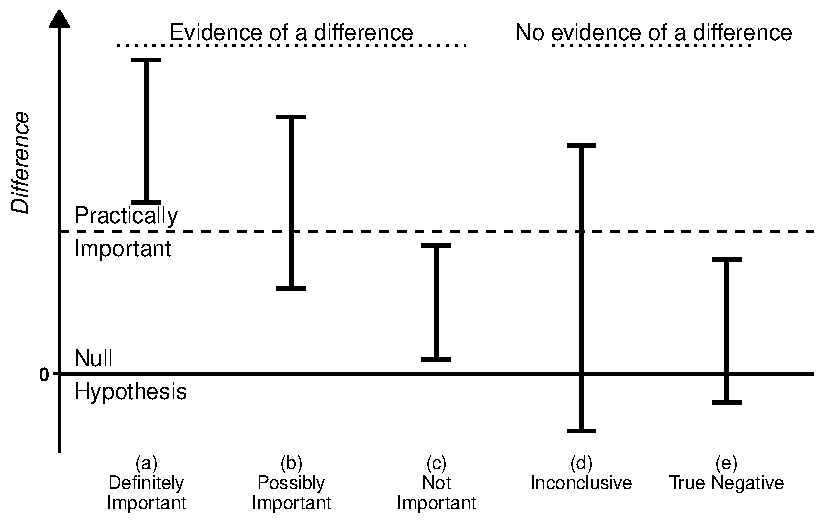
\includegraphics[keepaspectratio,alt={Five vertical confidence interval plots illustrate the distinction between statistical significance and practical importance. A solid horizontal line at zero represents the null hypothesis, while a dashed horizontal line above zero marks the threshold for a clinically or practically important effect. Intervals (a) and (b) lie entirely above zero, indicating statistically significant results; however, only (a) is clearly practically important because the entire interval is above the importance threshold, while (b) includes values of uncertain practical importance. Interval (c) is statistically significant because it does not cross zero, but it lies below the practical importance threshold, indicating a statistically significant yet clinically unimportant effect. Interval (d) crosses zero and spans both harmful and beneficial values, representing a statistically non-significant and inconclusive result. Interval (e) also crosses zero but remains below the practical importance threshold, suggesting a true negative result with no clinically important effect.}]{04-hypothesis-testing_files/figure-pdf/fig-practical-importance-1.pdf}}

}

\caption{\label{fig-practical-importance}}

\end{figure}%

It is possible when conducting significance tests, particularly in very
large studies, that a small difference provides strong evidence of an
effect due to increased precision from large sample sizes. For example,
in a large study of over 1000 patients, a new medication may be found to
lower blood pressure by an average of 1 mmHg more than a currently
accepted drug, providing strong evidence of a difference (P \textless{}
0.01). However, such a small reduction in blood pressure would be
unlikely to be practically important. The cost and potential side
effects of the new medication would need to be weighed against this very
small average benefit. In this situation, despite strong statistical
evidence, the finding would not be practically important. This is the
situation described in scenario (c) of
Figure~\ref{fig-practical-importance}.

Conversely, it is possible to obtain a large, practically important
difference between groups that provides little evidence of a difference.

For example, consider a small study to measure the rate of hospital
admissions following presentation to the Emergency Department. We may
find that 80\% of children who present to the Emergency Department are
admitted before the intervention, compared to only 65\% of children
after the intervention. However, the P value may be calculated as 0.38,
providing no evidence of a difference. This may be because only a small
number of participants were recruited in each period. Here, the
reduction in the admission rate by 15\% represents a practically
important difference, but not statistically significant. This situation
is represented in scenario (d) of Figure~\ref{fig-practical-importance}.

The important thing to remember is that statistical significance does
not always correspond to practical importance. A statistically
significant result may be practically unimportant, and a statistically
non-significant results may be practically important.

\section{Errors in significance
testing}\label{errors-in-significance-testing}

There are two conclusions we can draw when conducting a hypothesis test:
if the P-value is small, there is strong evidence against the null
hypothesis and we reject the null hypothesis. If the P-value is not
small, there is little evidence against the null hypothesis and we fail
to reject the null hypothesis. As discussed above, the ``small''
cut-point for the P-value is often taken as 0.05. We refer to this value
as \(\alpha\) (alpha).

We can conduct a thought experiment and compare our hypothesis test
conclusion to reality. In reality, either the null hypothesis is true,
or it is false. Of course, if we knew what reality was, we would not
need to conduct a hypothesis test. But we can compare our possible
hypothesis test conclusions to the true (unobserved) reality.

If the null hypothesis was true in reality, our hypothesis test can fail
to reject the null hypothesis -- this would be a correct conclusion.
However, the hypothesis test could lead us to rejecting the null
hypothesis -- this would be an incorrect conclusion. We call this
scenario a Type I error, and it has a probability of \(\alpha\).

The other situation is where, in reality, the null hypothesis is false.
A correct conclusion would be where our hypothesis test rejects the null
hypothesis. However, if our hypothesis test fails to reject the null
hypothesis, we have made a Type II error. The probability of making a
Type II error is denoted \(\beta\) (beta). We will see in Module 10 that
\(\beta\) is determined by the size of the study.

The error in falsely rejecting the null hypothesis when it is true (type
I error), or in falsely accepting the null hypothesis when it is not
true (type II error) is summarised in Table~\ref{tbl-mod4-alpha-beta}.
We will return to these concepts in Module 10, when discussing how to
determine the appropriate sample size of a study.

\begin{longtable}[]{@{}
  >{\raggedright\arraybackslash}p{(\linewidth - 4\tabcolsep) * \real{0.3056}}
  >{\centering\arraybackslash}p{(\linewidth - 4\tabcolsep) * \real{0.4028}}
  >{\centering\arraybackslash}p{(\linewidth - 4\tabcolsep) * \real{0.2917}}@{}}
\caption{Comparison of study result with the
truth}\label{tbl-mod4-alpha-beta}\tabularnewline
\toprule\noalign{}
\begin{minipage}[b]{\linewidth}\raggedright
\end{minipage} & \begin{minipage}[b]{\linewidth}\centering
\textbf{Effect in reality}
\end{minipage} & \begin{minipage}[b]{\linewidth}\centering
\textbf{No effect in reality}
\end{minipage} \\
\midrule\noalign{}
\endfirsthead
\toprule\noalign{}
\begin{minipage}[b]{\linewidth}\raggedright
\end{minipage} & \begin{minipage}[b]{\linewidth}\centering
\textbf{Effect in reality}
\end{minipage} & \begin{minipage}[b]{\linewidth}\centering
\textbf{No effect in reality}
\end{minipage} \\
\midrule\noalign{}
\endhead
\bottomrule\noalign{}
\endlastfoot
\textbf{Evidence was found} & Correct: Power (\(1 - \beta\)) & Error:
\(\alpha\) \\
\textbf{No evidence was found} & Error: \(\beta\) & Correct \\
\end{longtable}

\section{One-sample t-test}\label{one-sample-t-test}

A one-sample t-test tests whether a sample mean is different to a
hypothesised value. The t-distribution and its relation to normal
distribution has been discussed in detailed in Module 3.

In a one-sample t-test, a t-value is computed as the sample mean divided
by the standard error of the mean. The significance of the t-value is
then computed using software, or can be obtained from a statistical
table.

The principles of this test can be used for applications such as testing
whether the mean of a sample is different from a known population mean,
for example testing whether the IQ of a group of children is different
from the population mean of 100 IQ points or testing whether the number
of average hours worked in an adult sample is different from the
population mean of 38 hours.

\subsection{Worked Example}\label{worked-example-3}

The mean diastolic blood pressure (BP) of the general US population is
known to be 71 mm Hg. The diastolic blood pressure of 733 female Pima
indigenous Americans was measured and a density plot showed that the
data were approximately normally distributed. The mean diastolic blood
pressure in the sample was 72.4 mm Hg with a standard deviation of 12.38
mm Hg.

We can use jamovi or R to conduct a one sample t-test using the data
available (\texttt{mod04\_blood\_pressure.csv}). The results from this
test are summarised below.

\begin{longtable}[]{@{}
  >{\raggedright\arraybackslash}p{(\linewidth - 8\tabcolsep) * \real{0.1806}}
  >{\raggedright\arraybackslash}p{(\linewidth - 8\tabcolsep) * \real{0.1806}}
  >{\raggedright\arraybackslash}p{(\linewidth - 8\tabcolsep) * \real{0.1806}}
  >{\raggedright\arraybackslash}p{(\linewidth - 8\tabcolsep) * \real{0.1806}}
  >{\raggedright\arraybackslash}p{(\linewidth - 8\tabcolsep) * \real{0.2778}}@{}}
\caption{Summary of blood pressure from female Pima indigenous
Americans}\tabularnewline
\toprule\noalign{}
\begin{minipage}[b]{\linewidth}\raggedright
n
\end{minipage} & \begin{minipage}[b]{\linewidth}\raggedright
Mean
\end{minipage} & \begin{minipage}[b]{\linewidth}\raggedright
Standard deviation
\end{minipage} & \begin{minipage}[b]{\linewidth}\raggedright
Standard error
\end{minipage} & \begin{minipage}[b]{\linewidth}\raggedright
95\% confidence interval of the mean
\end{minipage} \\
\midrule\noalign{}
\endfirsthead
\toprule\noalign{}
\begin{minipage}[b]{\linewidth}\raggedright
n
\end{minipage} & \begin{minipage}[b]{\linewidth}\raggedright
Mean
\end{minipage} & \begin{minipage}[b]{\linewidth}\raggedright
Standard deviation
\end{minipage} & \begin{minipage}[b]{\linewidth}\raggedright
Standard error
\end{minipage} & \begin{minipage}[b]{\linewidth}\raggedright
95\% confidence interval of the mean
\end{minipage} \\
\midrule\noalign{}
\endhead
\bottomrule\noalign{}
\endlastfoot
733 & 72.4 & 12.38 & 0.46 & 71.5 to 73.3 \\
\end{longtable}

The test statistic for the one-sample t-test is calculated as
t\textsubscript{732}=3.07, with a P-value of 0.002.

The mean diastolic blood pressure of females from Pima is estimated as
72.4 mmHg (95\% CI: 71.5 to 73.3 mmHg), which is higher than that of the
general US population. Note that this interval does not contain the mean
of the general US population (71 mm Hg), providing some indication that
the mean diastolic blood pressure of female Pima people is higher than
that of the general US population.

The result from the formal hypothesis test gives strong evidence that
the mean diastolic BP of the female Pima people is higher than that of
the general US population (t\textsubscript{732}=3.07, P=0.002).

\section{One and two tailed tests}\label{one-and-two-tailed-tests}

Most statistical tests are two tailed tests, that is, we conduct a test
that allows for the summary statistic in the group of interest to be
either higher or lower than in the comparison group. For a t-test, this
requires that we obtain a two-tailed P value which gives us the
probability of the t-value being in either one of the two tails of the
t-distribution as shown in Figure~\ref{fig-two-tailed-test}. The shaded
regions show the t values that indicate a P value less than 0.05.

\begin{figure}

\centering{

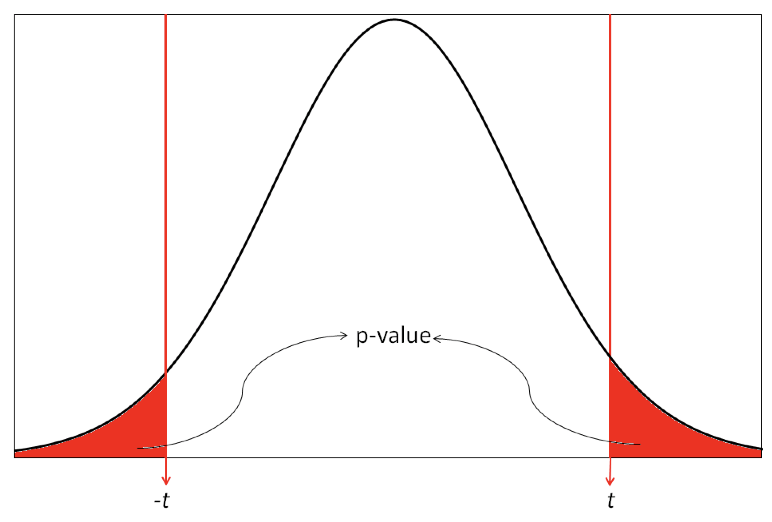
\includegraphics[width=0.66\linewidth,height=\textheight,keepaspectratio,alt={A symmetric bell-shaped t-distribution centred at zero. Both tails are shaded beyond the critical values, illustrating the rejection regions for a two-tailed hypothesis test with alpha equal to 0.05.}]{img/mod04/two-tailed-test.png}

}

\caption{\label{fig-two-tailed-test}P-value for a 2-tailed test}

\end{figure}%

Occasionally, one tailed tests are conducted in which the summary
statistic in the group of interest can only be higher or lower than the
comparison group, i.e.~a difference is specified to occur in one
direction only. In most studies, two tailed tests of significance are
used to allow for the possibility that the effect size could occur in
either direction. In clinical trials, this would mean allowing for a
result that can indicate a benefit or an adverse effect in response to a
new treatment. In epidemiological studies, two tailed tests are used to
allow for the fact that exposure to a factor of interest may be adverse
or may be beneficial. This conservative approach is usually adopted to
prevent missing important effects that occur in the opposite direction
to that expected by the researchers.

\section{A note on P-values displayed by
software}\label{a-note-on-p-values-displayed-by-software}

You will often see P-values generated by statistical software presented
as 0.000 or 0.0000. As P-values can never be equal to zero, any P-value
displayed in this way should be converted to \textless0.001 or
\textless0.0001 respectively (i.e.~replace the last 0 with a 1, and use
the less-than symbol).

R can display P-values in a very cryptic way: \(\text{6.478546e-05}\)
for example. This is translated as:

\[\begin{aligned}
6.478546e-05 &= 6.478546 \times 10^{-5} \\
  &= 6.478546 \times 0.00001 \\
  &= 0.00006478546
\end{aligned}\]

Such a P-value should be presented as P\textless0.0001.

\section{Decision Tree}\label{decision-tree}

In the following modules in this course, several formal statistical
tests will be described to analyse different types of data sets that
have been collected to test set null hypotheses. It is important that
the correct statistical test is selected to generate P-values and
estimate effect size. If an incorrect statistical test is used, the
assumptions of the test may be violated, the effect size may be biased
and the P value generated may be incorrect.

Selecting the correct test to use in each situation depends on the study
design and the nature of the variables collected. Figure 1 in the
Appendix shows a decision tree which enables you to decide the type of
test to select based on the nature of the data.

\section{Indigenous data sovereignty and governance: the Australian
context}\label{indigenous-data-sovereignty-and-governance-the-australian-context}

The issue of data sovereignty was raised in Module 3, and here we will
discuss how this concept applies in the Australian context.

Indigenous data encompasses information or knowledge in any format or
medium that is about, or may affect, Aboriginal and Torres Strait
Islander peoples, either collectively or individually. (Walter et al.
2021) Indigenous Data Sovereignty specifically refers to the right of
Aboriginal and Torres Strait Islander peoples, communities, and
organisations to maintain, control, protect, develop, and use data as it
relates to them. Data practices must support and enhance Indigenous
collective well-being.

Indigenous Data Governance provides the practical mechanisms through
which sovereignty is enacted. It consists of formal systems that assert
Indigenous data interests regarding how data is accessed and used,
ensuring that practices reflect Indigenous priorities, values, culture,
and diversity.(Walter et al. 2021) Importantly, Indigenous Data
Sovereignty is practised through Indigenous data governance, making
governance the operational expression of sovereignty principles.

\subsection{The Problem of Deficit-Based Data
Narratives}\label{the-problem-of-deficit-based-data-narratives}

A major challenge in Australian data collections is that First Nations
peoples are often framed as the ``object of study'' rather than as
active participants in research. Data frequently focuses on poor
outcomes across health, education, and economic participation, creating
what has been termed the ``5D data'' narrative: disparity, deprivation,
disadvantage, dysfunction, and difference. This approach has been
further characterised as BADDR Data: Blaming, Aggregate,
Decontextualised, Deficit, and Restricted.(Walter et al. 2021) Such
framings perpetuate harmful stereotypes and fail to capture the
strengths, resilience, and diversity of Indigenous communities.

\subsection{Key Principles for Indigenous Data
Management}\label{key-principles-for-indigenous-data-management}

Indigenous data management in Australia operates according to several
foundational principles. Indigenous data should be reflective of
Aboriginal and Torres Strait Islander interests, values, and cultural
ways, ensuring cultural appropriateness throughout the data lifecycle.
Data must be accessible and appropriate, meeting Indigenous needs rather
than serving external agendas. Collection practices must incorporate
free, prior, and informed consent, with respect for confidentiality
maintained throughout.

Secure storage of Indigenous data is essential, as is the requirement
that data be returned to communities in an easily understood and
meaningful way. Interpretation of Indigenous data should be conducted by
Aboriginal and Torres Strait Islander experts who possess the cultural
knowledge necessary for appropriate analysis. Finally, data use must
advance self-determination and development, and only proceed in ways
that Indigenous peoples agree to.

\subsection{FAIR and CARE Principles}\label{fair-and-care-principles}

The Australian Open Data infrastructure incorporates FAIR principles
(Findable, Accessible, Interoperable, Reusable) for scientific data,
which aim to maximise data use and reuse. However, these principles do
not mention or address the specific concerns of Indigenous peoples. To
address this gap, the CARE Principles for Indigenous Data Governance
have been developed to complement FAIR principles.

The CARE framework consists of four key components:

\begin{itemize}
\item
  Collective Benefit emphasises inclusive development and innovation,
  improved governance and citizen engagement, and equitable outcomes.
\item
  Authority to Control focuses on recognising Indigenous rights and
  interests, supporting data for governance, and enabling the governance
  of data itself.
\item
  Responsibility calls for positive relationships, expanding capability
  and capacity, and incorporating Indigenous worldviews into data
  practices.
\item
  Ethics stresses minimising harm and maximising benefit, promoting
  justice, and careful consideration of future data uses.
\end{itemize}

This framework enables the enactment of FAIR principles but with
appropriate care and attention to Indigenous rights and
interests.(Walter et al. 2021)

\subsection{Protecting Indigenous Data Sovereignty Rights in
Research}\label{protecting-indigenous-data-sovereignty-rights-in-research}

Aboriginal and Torres Strait Islander peoples have the right to decide
how Indigenous data is used and stored.{[}Lowitja Institute
(2021){]}(National Indigenous Australians Agency 2024) Formal agreements
protecting Indigenous Data Sovereignty should be established at the
outset of any research project. Such agreements must cover intellectual
property rights, data collection procedures, retention and access
arrangements, and management protocols for all data arising from the
research. These agreements must also specify actions that Aboriginal and
Torres Strait Islander peoples, communities, and organisations can take
if commitments are not met. Crucially, these agreements must be clearly
understood and formally endorsed by appropriate representatives of the
involved Aboriginal and Torres Strait Islander peoples, communities, and
organisations.

First Nations peoples have the right to lead and participate at all
stages of the research process, including planning, data collection,
analysis, dissemination of results, return of data, and ongoing access
to data. Researchers bear responsibility for providing appropriate
information to promote full and effective Indigenous leadership in data
collection. They must also provide opportunities for communities to
assess data collection, storage, and governance arrangements, including
confidentiality protections. Indigenous peoples must have opportunities
to engage in the development, design, collection, analysis, and
reporting of data, including involvement in the development of
appropriate indicators and surveys applicable to local contexts.

\newpage{}

\bookmarksetup{startatroot}

\chapter*{Jamovi notes}\label{jamovi-notes-2}
\addcontentsline{toc}{chapter}{Jamovi notes}

\markboth{Jamovi notes}{Jamovi notes}

\section{One sample t-test}\label{one-sample-t-test-1}

We will use data from \texttt{mod04\_blood\_pressure.csv} to demonstrate
how a one-sample t-test is conducted in Jamovi. To perform the test, go
to \textbf{Analyses \textgreater{} T-Tests \textgreater{} One Sample
T-Test}.

Select \texttt{dbp} as the \textbf{Dependent Variable}. Enter the
hypothesised mean as the \textbf{Test value} (\texttt{71} in this
example) as shown below.

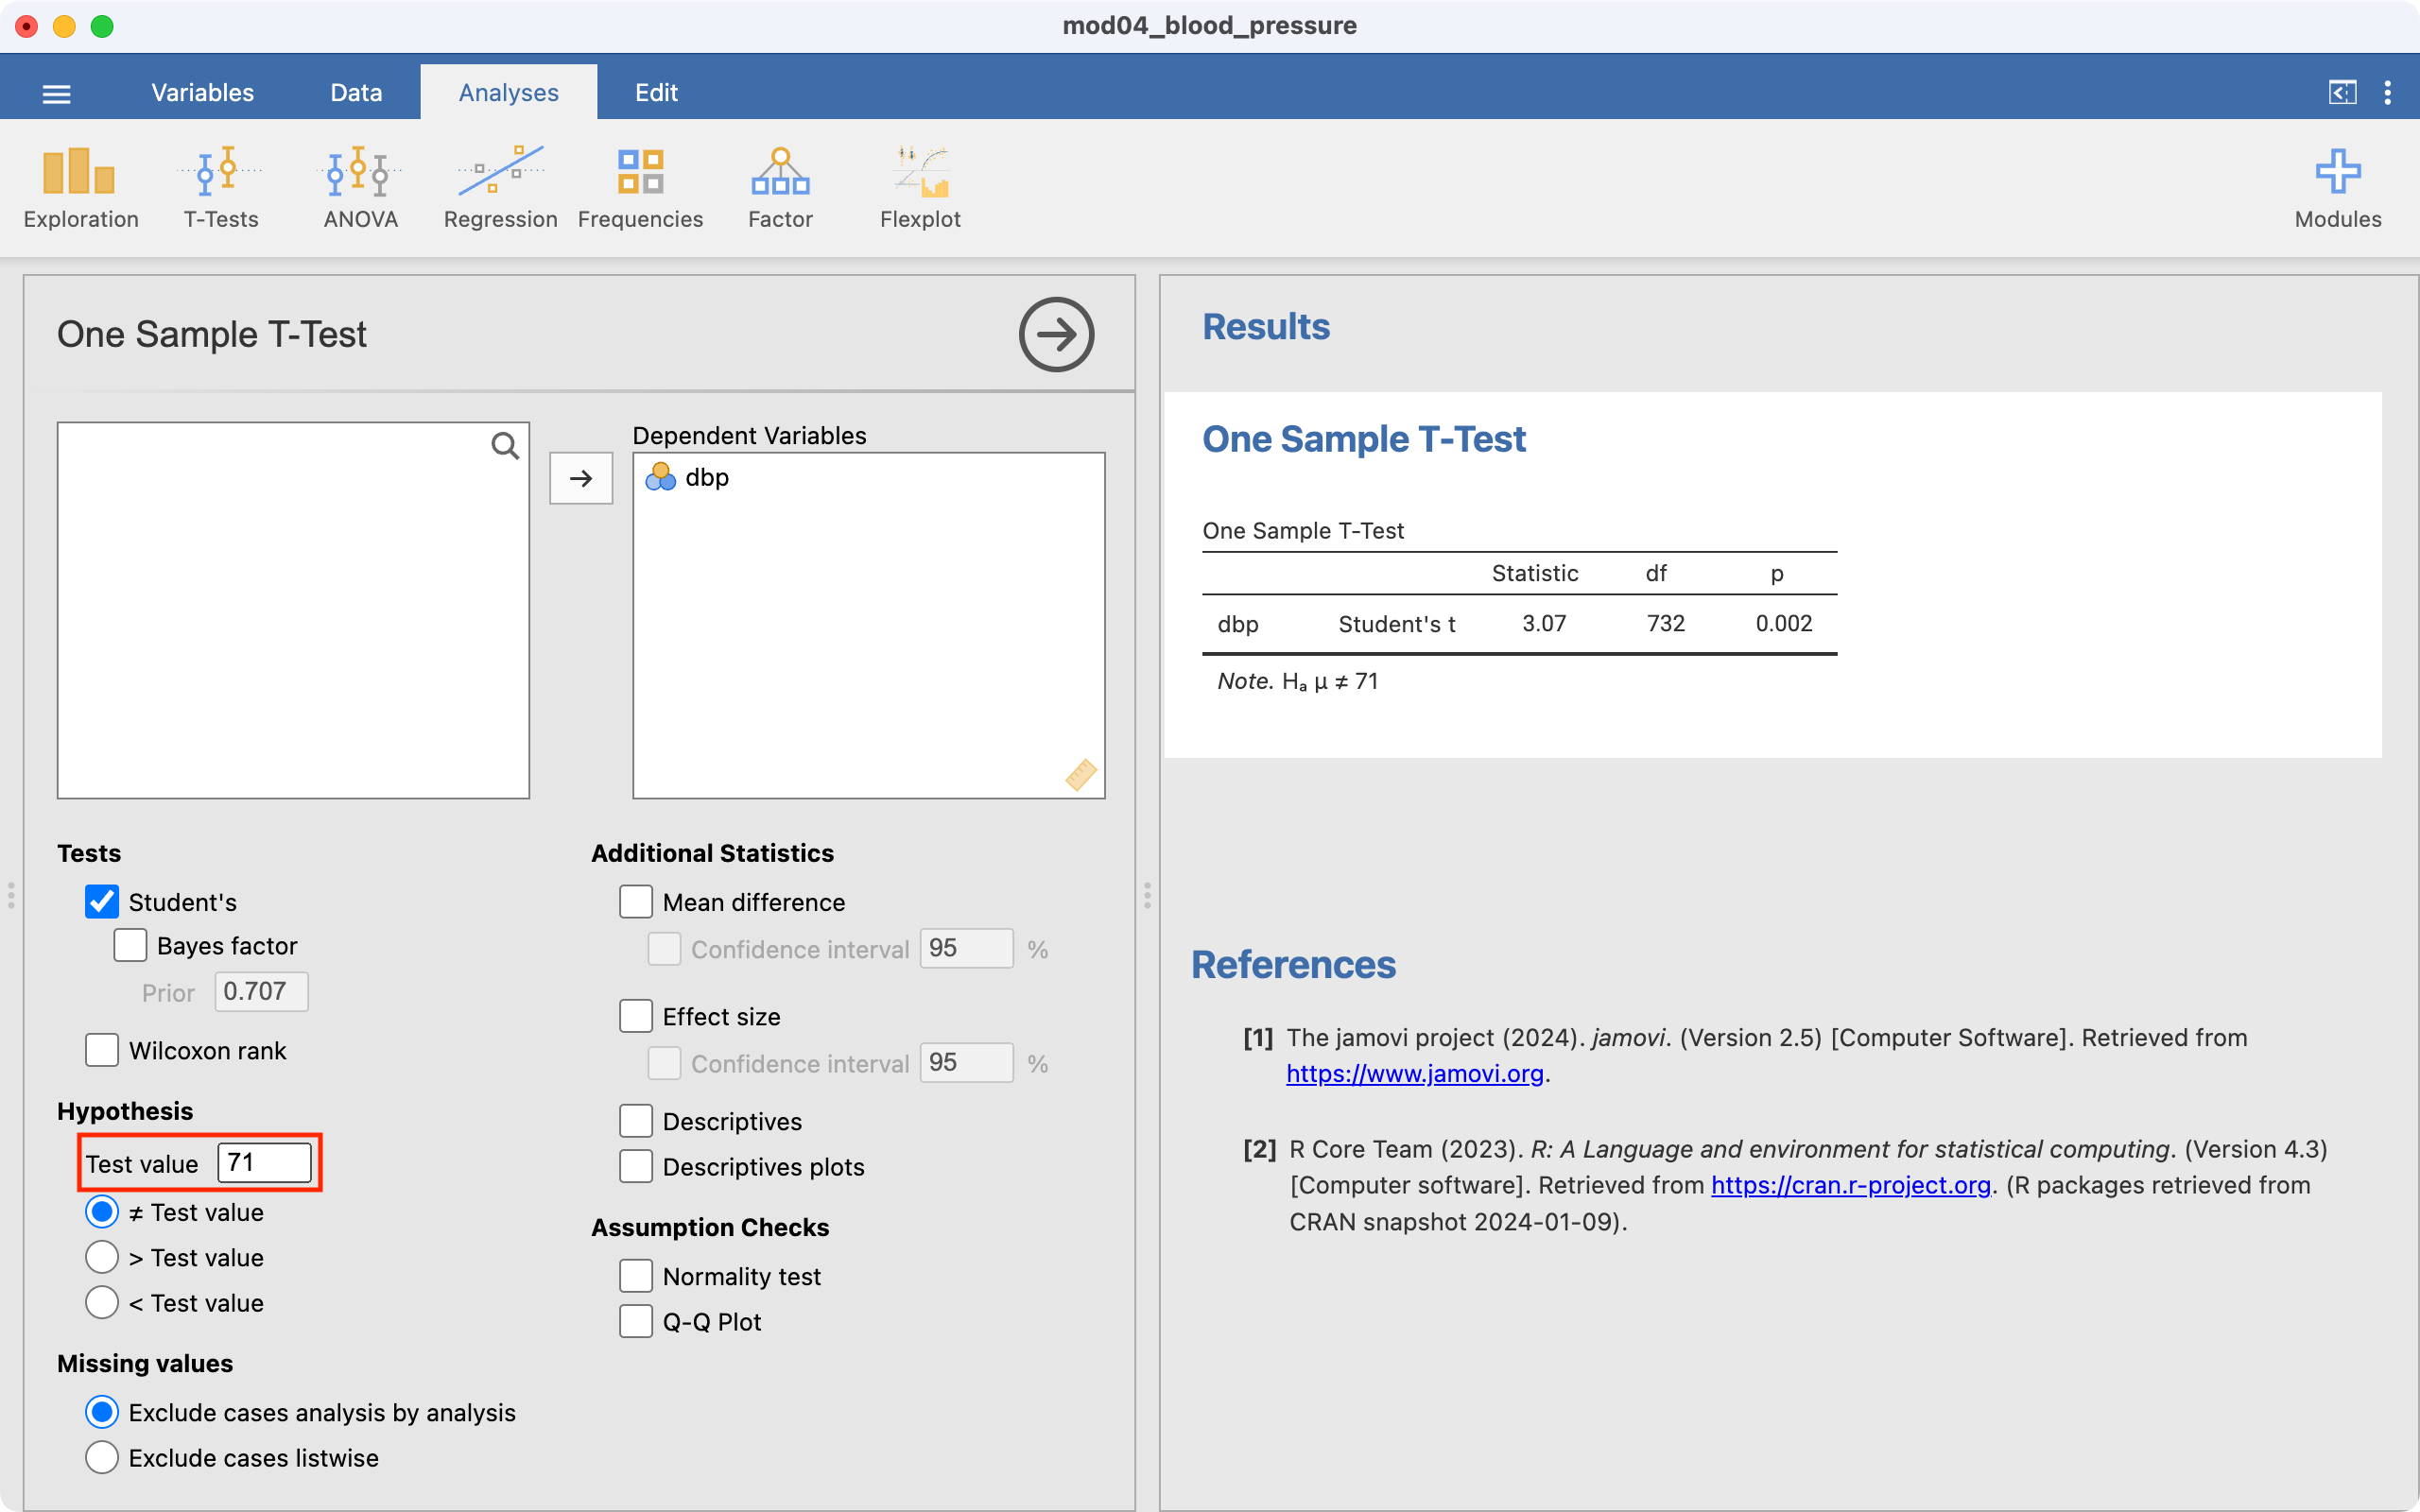
\includegraphics[width=1\linewidth,height=\textheight,keepaspectratio]{img/mod04/jamovi/mod4-ttest.png}

The test statistic (i.e.~t and its degrees of freedom) are provided. By
default, Jamovi will calculate a P-value for the two-sided test
(H\textsubscript{a}: mean \(\neq\) 71), which appropriate for this
example.

Note that the one-sample t-test output does not include the mean or the
95\% confidence interval of the mean of your variable of interest. This
should be obtained using \textbf{Exploration \textgreater{}
Descriptives}:

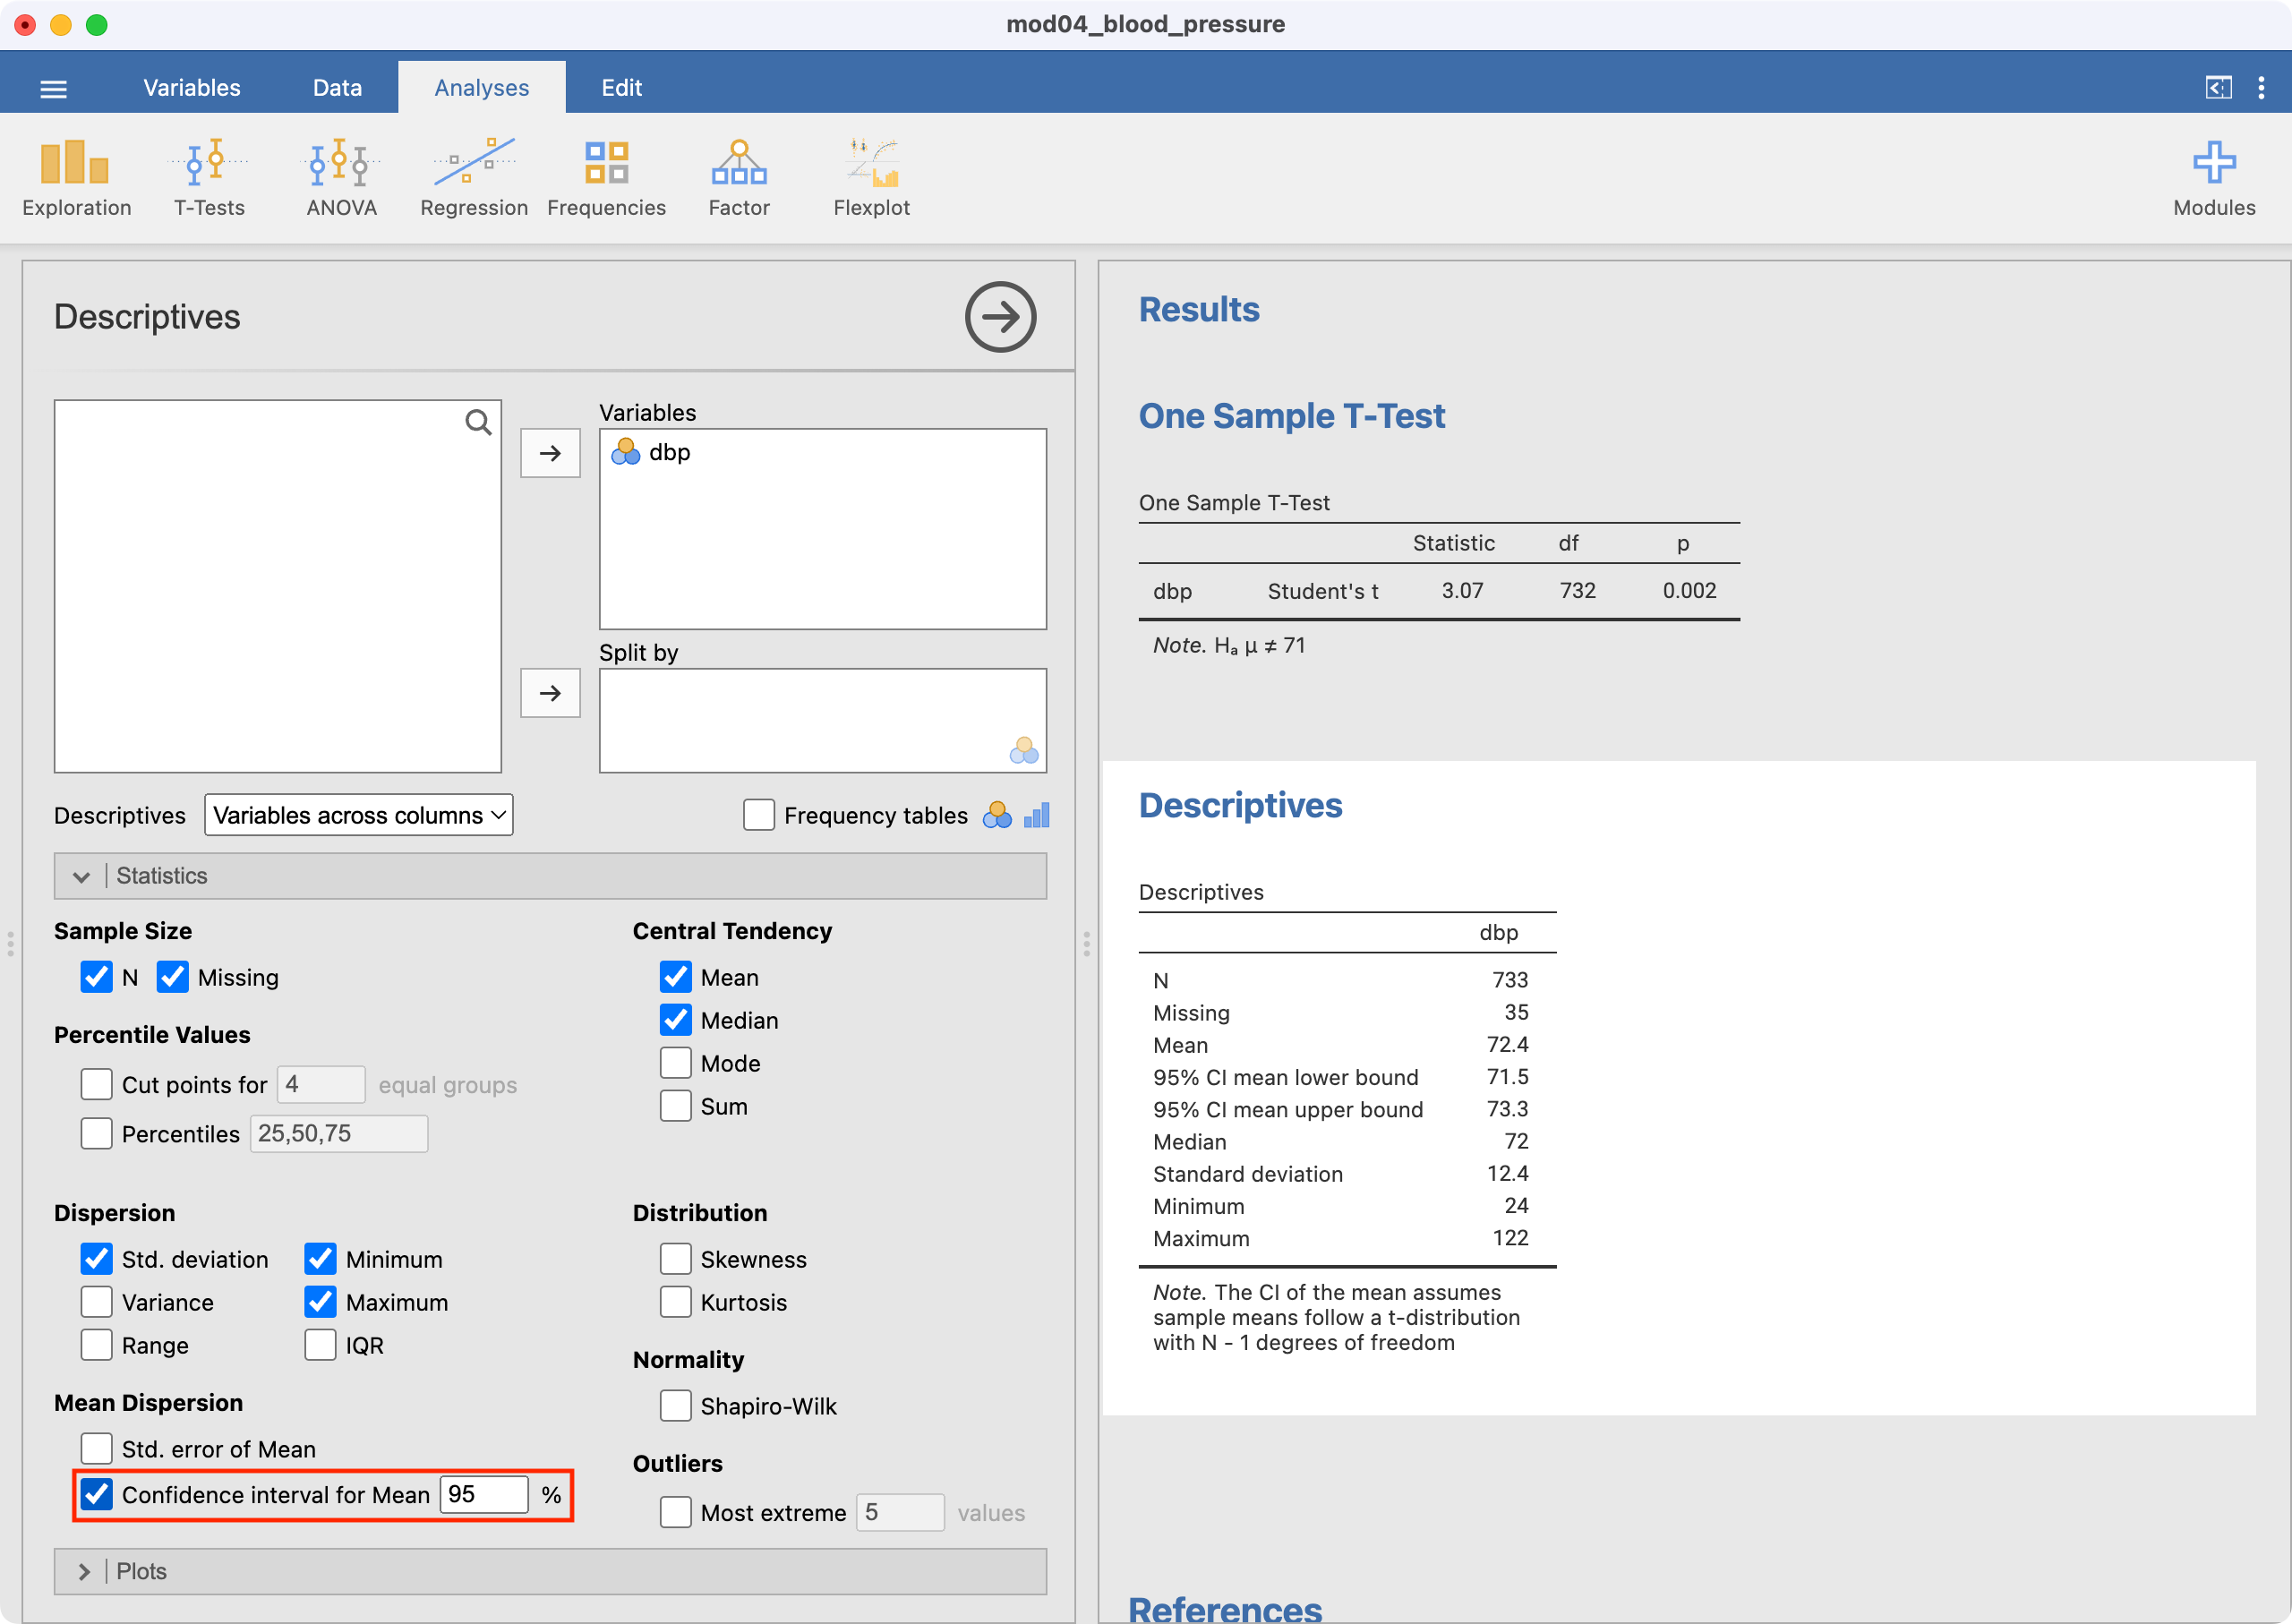
\includegraphics[width=1\linewidth,height=\textheight,keepaspectratio]{img/mod04/jamovi/mod4-ttest-desc.png}

\newpage{}

\bookmarksetup{startatroot}

\chapter*{R notes}\label{r-notes-2}
\addcontentsline{toc}{chapter}{R notes}

\markboth{R notes}{R notes}

\section{One sample t-test}\label{one-sample-t-test-2}

We will use data from \texttt{mod04\_blood\_pressure.csv} to demonstrate
how a one-sample t-test is conducted in R. To test whether the mean
diastolic blood pressure of the population from which the sample was
drawn is equal to 71, we can use the t.test command:

\begin{Shaded}
\begin{Highlighting}[]
\NormalTok{pima }\OtherTok{\textless{}{-}} \FunctionTok{read.csv}\NormalTok{(}\StringTok{"data/examples/mod04\_blood\_pressure.csv"}\NormalTok{)}
\FunctionTok{t.test}\NormalTok{(pima}\SpecialCharTok{$}\NormalTok{dbp, }\AttributeTok{mu=}\DecValTok{71}\NormalTok{)}
\end{Highlighting}
\end{Shaded}

\begin{verbatim}

    One Sample t-test

data:  pima$dbp
t = 3.0725, df = 732, p-value = 0.002202
alternative hypothesis: true mean is not equal to 71
95 percent confidence interval:
 71.50732 73.30305
sample estimates:
mean of x 
 72.40518 
\end{verbatim}

The output provides:

\begin{itemize}
\tightlist
\item
  a test statistic (t=3.07);
\item
  degrees of freedom for the test statistic (df = 732);
\item
  a P-value from the two-sided test (P=0.002);
\item
  the mean of the sample (72.4);
\item
  and the 95\% confidence interval of the mean (71.5 to 73.3).
\end{itemize}

\newpage{}

\bookmarksetup{startatroot}

\chapter*{Activities}\label{activities-3}
\addcontentsline{toc}{chapter}{Activities}

\markboth{Activities}{Activities}

\subsection*{Activity 4.1}\label{activity-4.1}
\addcontentsline{toc}{subsection}{Activity 4.1}

It has been suggested that the average Australian consumes around 8700
kJ per day. A study was conducted to estimate the average dietary
consumption of Australian males, aged between 30 and 50. The mean
dietary intake was estimated as 9461 kJ, with a 95\% confidence interval
from 8879 to 10043 kJ. What can you conclude about the dietary
consumption of Australian males from this study?

\subsection*{Activity 4.2}\label{activity-4.2}
\addcontentsline{toc}{subsection}{Activity 4.2}

Women attending a GP clinic were asked to complete a health survey. Data
from 154 responses are saved in \texttt{Activity\_4.2.csv}. The file
contains the following variables:

\begin{itemize}
\tightlist
\item
  id: participant ID number
\item
  age: age in years
\item
  height: height in cm
\item
  weight: weight in kg
\item
  waist: waist circumference in cm
\end{itemize}

Australia's National Health Survey has estimated the Australian female
population has a mean waist circumference of 87.9cm. Analyse the health
survey data to compare women attending a GP clinic to the Australian
population.

\subsection*{Activity 4.3}\label{activity-4.3}
\addcontentsline{toc}{subsection}{Activity 4.3}

Setting the significance level at P \textless{} 0.10 instead of the more
usual P \textless{} 0.05 increases the likelihood of:

\begin{enumerate}
\def\labelenumi{\alph{enumi})}
\tightlist
\item
  a Type I error
\item
  a Type II error
\item
  rejecting the null hypothesis
\item
  not rejecting the null hypothesis
\end{enumerate}

\subsection*{Activity 4.4}\label{activity-4.4}
\addcontentsline{toc}{subsection}{Activity 4.4}

For a fixed sample size setting the significance level at a very extreme
cutoff such as P \textless{} 0.001 increases the chances of:

\begin{enumerate}
\def\labelenumi{\alph{enumi})}
\tightlist
\item
  obtaining a significant result
\item
  rejecting the null hypothesis
\item
  a Type I error
\item
  a Type II error
\end{enumerate}

\bookmarksetup{startatroot}

\chapter{Comparing the means of two
groups}\label{comparing-the-means-of-two-groups}

\section*{Learning objectives}\label{learning-objectives-4}
\addcontentsline{toc}{section}{Learning objectives}

\markright{Learning objectives}

By the end of this module you will be able to:

\begin{itemize}
\tightlist
\item
  Decide whether to use an independent samples t-test or a paired t-test
  to compare two the means of two groups;
\item
  Conduct and interpret the results from an independent samples t-test;
\item
  Describe the assumptions of an independent samples t-test;
\item
  Conduct and interpret the results from a paired t-test;
\item
  Describe the assumptions of a paired t-test;
\item
  Conduct an independent samples t-test and a paired t-test using
  software;
\item
  Report results and provide a concise summary of the findings of
  statistical analyses.
\end{itemize}

\section*{Optional readings}\label{optional-readings-4}
\addcontentsline{toc}{section}{Optional readings}

\markright{Optional readings}

Kirkwood and Sterne (2001); Sections 7.1 to 7.5.
\href{http://er1.library.unsw.edu.au/er/cgi-bin/eraccess.cgi?url=https://ebookcentral.proquest.com/lib/unsw/detail.action?docID=624728}{{[}UNSW
Library Link{]}}

Bland (2015); Section 10.3.
\href{http://er1.library.unsw.edu.au/er/cgi-bin/eraccess.cgi?url=https://ebookcentral.proquest.com/lib/unsw/detail.action?docID=5891730}{{[}UNSW
Library Link{]}}

\section{Introduction}\label{introduction-4}

In Module 4, a one-sample t-test was used for comparing a single mean to
a hypothesised value. In health research, we often want to compare the
means between two groups. For example, in an observational study, we may
want to compare cholesterol levels in people who exercise regularly to
the levels in people who do not exercise regularly. In a clinical trial,
we may want to compare cholesterol levels in people who have been
randomised to a dietary modification or to usual care. In this module,
we show how to compare the means of two groups where the analysis
variable is normally distributed.

From the decision tree presented in the Appendix, we can see that if we
have a continuous outcome measure and two categorical groups that are
not related, i.e.~a binary exposure measurement, the test for such data
is an independent samples t-test. The test is also sometimes called a
2-sample t-test.

In research, data are often `paired' or `matched', that is the two data
points are related to one another. This occurs when measurements are
taken:

\begin{itemize}
\tightlist
\item
  From each participant on two occasions, e.g.~at baseline and follow-up
  in an experimental study or in a longitudinal cohort study;
\item
  From related people, e.g.~a mother and daughter or a child and their
  sibling;
\item
  From related sites in the same person, e.g.~from both limbs, eyes or
  kidneys;
\item
  From matched participants e.g.~in a matched case-control study;
\item
  In cross-over clinical trials where the patient receives both drugs,
  often in random order.
\end{itemize}

An independent samples t-test cannot be used for analysing paired or
matched data because the assumption that the two groups are independent
is violated. Treating paired or matched measurements as independent
samples would artificially inflate the sample size and lead to
inaccurate P values. When the data are related in a paired or matched
way and the outcome is continuous, a paired t-test is the appropriate
statistic to use if the data are normally distributed.

\section{Independent samples t-test}\label{independent-samples-t-test}

An independent samples t-test is a parametric test that is used to
assess whether the mean values of two groups are different from one
another. Thus, the test is used to assess whether two mean values are
similar enough to have come from the same population or whether the
difference between them is so large that the two groups can be
considered to have come from separate populations with different
characteristics.

The null hypothesis is that the mean values of the two groups are not
different, that is:

H\textsubscript{0}: (\(\mu_1 - \mu_2\)) = 0

Rejecting the null hypothesis using an independent samples t-test
indicates that the difference between the means of the two groups is
large in relation to the variability in the samples and is unlikely to
be due to chance or to sampling variation.

\subsection{Assumptions for an independent samples
t-test}\label{assumptions-for-an-independent-samples-t-test}

The assumptions that must be met before an independent samples t-test
can be used are:

\begin{itemize}
\tightlist
\item
  The two groups are independent
\item
  The measurements are independent
\item
  The analysis variable must be continuous and must be normally
  distributed in each group
\end{itemize}

The first two assumptions are determined by the study design. The two
samples must be independent, i.e.~if a person is in one group then they
cannot be included in the other group, and the measurements within a
sample must be independent, i.e.~each person must be included in their
group once only.

The third assumption of normality is important although t-tests are
robust to some degree of non-normality as long as there are no
influential outliers and, more importantly, if the sample size is large.
We examined how to assess normality in Module 2. If the data are not
normally distributed, it may be possible to transform them using a
mathematical function such as a logarithmic transformation. If not, then
we may need to use non-parametric tests. This is examined in Module 9.

Traditionally, the variance of the analysis variable in each group was
assumed to be equal. However, this assumption can be relaxed by using
Welch's variation of the t-test. It has been recommended that this
unequal-variances t-test be used in most, if not all situations (West
2021; Delacre et al. 2017; Ruxton 2006).

\subsection{Worked Example 5.1}\label{worked-example-5.1}

In an observational study of a random sample of 100 full term babies
from the community, birth weight and gender were measured. There were 44
male babies and 56 female babies in the sample. The research question
asked whether there was a difference in birth weights between boys and
girls. The two groups are independent of each other and therefore an
independent samples t-test can be used to test the null hypothesis that
there is no difference in weight between the genders.

Exploratory data analysis of the variable of interest in each group
should always be obtained before a t-test is undertaken to ensure that
the assumptions are met. In particular, the distribution of the analysis
variable should be examined for each group, as shown in
Figure~\ref{fig-mod05-bwt-gender}. The data are stored in
\texttt{mod05\_birthweight.rds}.

\begin{figure}

\centering{

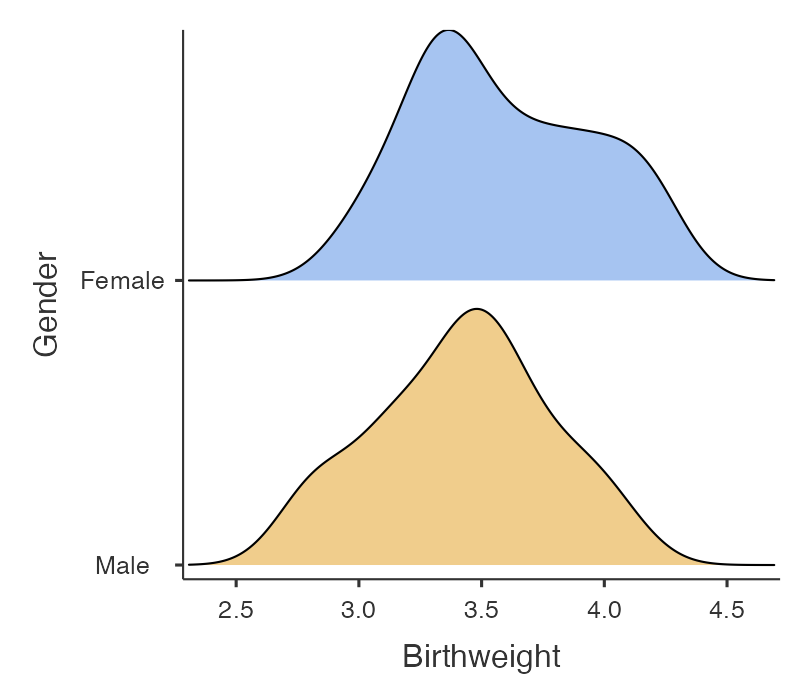
\includegraphics[width=0.5\linewidth,height=\textheight,keepaspectratio]{img/mod05/mod05-bwt-gender.png}

}

\caption{\label{fig-mod05-bwt-gender}Distribution of birth weight by
gender}

\end{figure}%

The plots show that the data are approximately normally distributed: the
density curves are relatively bell shaped and symmetric, and there are
no outliers.

We can also describe the data using summary statistics:

\begin{table}[h]

\caption{\label{tbl-5-1}Summary of birthweight by gender}

\centering{

\centering
\begin{tblr}[         %% tabularray outer open
]                     %% tabularray outer close
{                     %% tabularray inner open
colspec={Q[]Q[]Q[]},
hline{2}={1-3}{solid, black, 0.05em},
hline{1}={1-3}{solid, black, 0.08em},
hline{6}={1-3}{solid, black, 0.08em},
}                     %% tabularray inner close
& Female & Male \\
Number & 56 & 44 \\
Mean (SD) & 3.59 (0.36) & 3.42 (0.35) \\
Median (Q1, Q3) & 3.53 (3.32, 3.88) & 3.43 (3.15, 3.63) \\
Range & 2.95 to 4.25 & 2.75 to 4.10 \\
\end{tblr}

}

\end{table}%

The table shows that girls have a mean weight of 3.59 kg (SD 0.36) and
boys have a mean weight of 3.42 kg (SD 0.35) with females being heavier
than males. The variabilities of birth weight (i.e.~the standard
deviation) are similar between the two groups.

\subsection{Conducting and interpreting an independent samples
t-test}\label{conducting-and-interpreting-an-independent-samples-t-test}

An independent samples t-test provides us with a t statistic from which
we can compute a P value. The computation of the t statistic is as
follows:

\[t = \frac{{\overline{x}}_{1} - {\overline{x}}_{2}}{SE({\overline{x}}_{1} - {\overline{x}}_{2})}\]

with the standard error and degrees of freedom calculated from software.
Note that by using Welch's t-test, the degrees of freedom will usually
not be a whole number, and will appear with decimals.

Looking at the formula for the t-statistic, we can see that the \(t\) is
an estimate of how different the mean values are compared to the
variability of the difference in means. So \(t\) will become larger as
the difference in means increases with respect to the variability.

Statistical software will calculate both the t and P values. If the
t-value is large, the P value will be small, providing evidence against
the null hypothesis of no difference between the groups.

Table~\ref{tbl-ind-t} summarises the results of an independent samples
t-test using \texttt{mod05\_birthweight.rds}. The process of conducting
the t-test is summarised for jamovi and R in the following sections.

\begin{table}[h]

\caption{\label{tbl-ind-t}Birthweight (kg) by sex}

\centering{

\centering
\begin{tblr}[         %% tabularray outer open
]                     %% tabularray outer close
{                     %% tabularray inner open
colspec={Q[]Q[]Q[]Q[]},
hline{2}={1-4}{solid, black, 0.05em},
hline{1}={1-4}{solid, black, 0.08em},
hline{5}={1-4}{solid, black, 0.08em},
}                     %% tabularray inner close
Sex & n & Mean (SE) & 95\% Confidence Interval \\
Female & 56 & 3.59 (0.049) & 3.49 to 3.68 \\
Male & 44 & 3.42 (0.053) & 3.31 to 3.53 \\
Difference & NA & 0.17 (0.072) & 0.02 to 0.31 \\
\end{tblr}

}

\end{table}%

Here we see that girls are heavier than boys, and the mean difference in
weights between the genders is 0.17 kg (95\% CI 0.02, 0.31). We are 95\%
confident that the true mean difference of weight between girls and boys
lies between 0.02 and 0.31 kg. Note that this interval does not contain
the null value of 0.

Here we are testing the null hypothesis of no difference in mean
birthweights between females and males: a two-sided test. The t-value is
calculated as 2.30 with 93.5 degrees of freedom, and yields a two-sided
P value of 0.023, providing evidence of a difference in mean birthweight
between sex.

\section{Paired t-tests}\label{paired-t-tests}

If the outcome of interest is the difference in the continuously outcome
measurement between each pair of observations, a paired t-test is used.
In effect, a paired t-test is used to assess whether the mean of the
differences between the two related measurements is significantly
different from zero. In this sense, a paired t-test is very closely
aligned with a one sample t-test.

When using a paired t-test, the variation \emph{between the pairs} of
measurements is the most important statistic. The variation between the
participants is of little interest.

For related measurements, the data for each pair of values must be
entered on the same row of the spreadsheet. Thus, the number of rows in
the data sheet is the number of pairs of observations. Thus, the
effective sample size is the total number of pairs and not the total
number of measurements.

\subsection{Assumptions for a paired
t-test}\label{assumptions-for-a-paired-t-test}

The assumptions for a paired t-test are:

\begin{itemize}
\tightlist
\item
  the outcome variable is continuous
\item
  the differences between the pair of the measurements are normally
  distributed
\end{itemize}

For a paired samples t-test, it is important to test whether the
\emph{differences} between the two measurements are normally
distributed. If the assumptions for a paired t-test cannot be met, a
non-parametric equivalent is a more appropriate test to use (Module 9).

\subsection{Computing a paired t-test}\label{computing-a-paired-t-test}

The null hypothesis for using a paired t-test is as follows:

H\textsubscript{0}: Mean (Measurement1 -- Measurement2) = 0

To compute a t-value, the size of the mean difference between the two
measurements is compared to the standard error of the paired
differences, i.e.

\[t = \frac{\overline{d}}{SE(\overline{d})}\]

with \emph{n}--1 degrees of freedom, where \emph{n} is the number of
pairs.

Because the standard error becomes smaller as the sample size becomes
larger, the t-value increases as the sample size increases for the same
mean difference.

\subsection{Worked Example 5.2}\label{worked-example-5.2}

A total of 107 people were recruited into a study to assess whether
ankle blood pressure measured in two different sites would be the same.
For each person, systolic blood pressure (SBP) was measured in two
sites: dorsalis pedis and tibialis posterior.

Using the dataset \texttt{mod05\_ankle\_bp.xlsx}, we first need to
compute the pairwise difference between SBP measured in the two sites.
The distribution of the difference between SBP measured in dorsalis
pedis and tibialis posterior is shown in Figure~\ref{fig-mod05-sbpdiff}.
The differences approximate a normal distribution and therefore a paired
t-test can be used.

\begin{figure}

\centering{

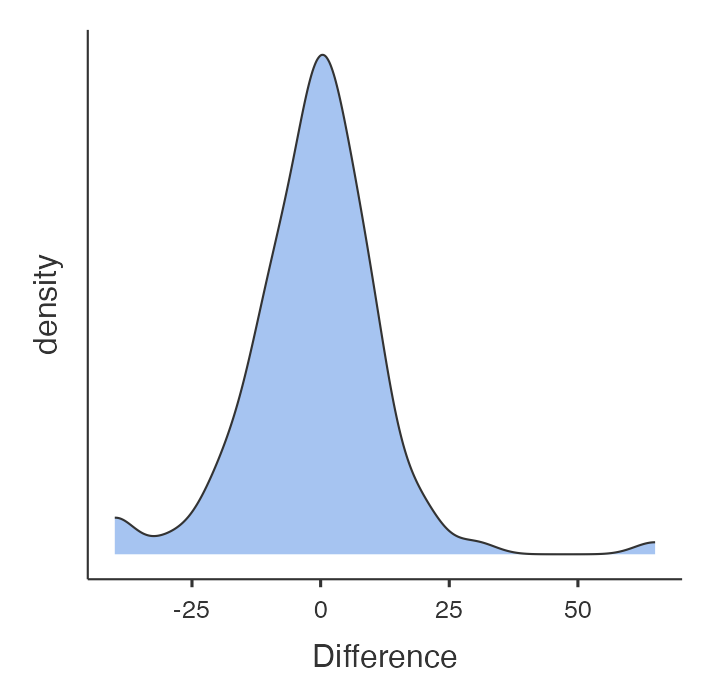
\includegraphics[width=0.5\linewidth,height=\textheight,keepaspectratio]{img/mod05/mod05-sbpdiff.png}

}

\caption{\label{fig-mod05-sbpdiff}Distribution of differences in ankle
SBP between two sites of 107 participants}

\end{figure}%

The paired t-test can be performed using statistical software, with a
summary of the results presented in Table~\ref{tbl-paired-t}. We can see
that the mean SBP is very similar in the two sites.

\begin{table}[h]

\caption{\label{tbl-paired-t}Systolic blood pressure (mmHg) measured at
two sites on the ankle}

\centering{

\centering
\begin{tblr}[         %% tabularray outer open
]                     %% tabularray outer close
{                     %% tabularray inner open
colspec={Q[]Q[]Q[]Q[]},
hline{2}={1-4}{solid, black, 0.05em},
hline{1}={1-4}{solid, black, 0.08em},
hline{5}={1-4}{solid, black, 0.08em},
}                     %% tabularray inner close
Site & n & Mean (SE) & 95\% Confidence Interval \\
Dorsalis pedis & 107 & 116.7 (3.46) & (109.9 to 123.6) \\
Tibialis posterior & 107 & 118.0 (3.43) & (111.2 to 124.8) \\
Difference & 107 & -1.3 (1.31) & (-3.9 to 1.3) \\
\end{tblr}

}

\end{table}%

The t-value is calculated as −0.96 with 106 degrees of freedom,
providing a two-sided P-value of 0.34. Thus these data provide no
evidence of a difference in systolic blood pressure between the two
sites.

\section{Confidence intervals in hypothesis
testing}\label{confidence-intervals-in-hypothesis-testing}

In Module 3, the 95\% confidence interval around a mean value was
calculated to show the precision of the summary statistic. The 95\%
confidence intervals around other summary statistics can also be
calculated.

For example, if we were comparing the means of two groups, we would want
to test the null hypothesis that the difference in means is zero, that
there is no true difference between the groups.

From the data from the two groups, we could estimate the difference in
means, the standard error of the difference in means and the 95\%
confidence interval around the difference. To estimate the 95\%
confidence interval, we use the formula given in Module 3, that is:

\[ 95\% \text{ CI} = \text{Difference in means} \pm 1.96 \times \text{SE}(\text{Difference in means)} \]

It is important to remember that the 95\% CI is estimated from the
standard error, and that the standard error has a direct relationship to
the sample size. For small sample sizes, the standard error is large and
the 95\% CI becomes wider. Conversely, the larger the sample size, the
smaller the standard error and the narrower the 95\% CI becomes
indicating a more precise estimate of the mean difference.

The 95\% CI tells us the region in which we are 95\% confident that the
true difference between the groups in the population lies. If this
region contains the null value of no difference, we can say that we are
95\% confident that there is no true difference between the groups and
therefore we would not reject the null hypothesis. This is shown in the
top two estimates in Figure~\ref{fig-cis-overlapping-null}. If the zero
value lies outside the 95\% confidence interval, we can conclude that
there is evidence of a difference between the groups because we are 95\%
confident that the difference does not encompass a zero value (as shown
in the lower two estimates in Figure~\ref{fig-cis-overlapping-null}).

\begin{figure}

\centering{

\pandocbounded{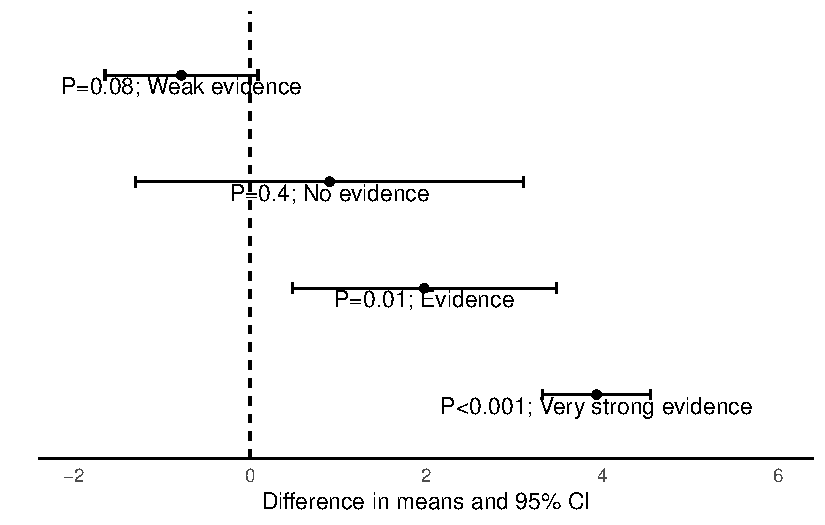
\includegraphics[keepaspectratio]{05-comparing-two-means_files/figure-pdf/fig-cis-overlapping-null-1.pdf}}

}

\caption{\label{fig-cis-overlapping-null}Using confidence intervals as
informal hypothesis tests}

\end{figure}%

\newpage{}

\bookmarksetup{startatroot}

\chapter*{Jamovi notes}\label{jamovi-notes-3}
\addcontentsline{toc}{chapter}{Jamovi notes}

\markboth{Jamovi notes}{Jamovi notes}

\section{Checking data for the independent samples
t-test}\label{checking-data-for-the-independent-samples-t-test}

\subsection{Examining variable distributions by a second
variable}\label{examining-variable-distributions-by-a-second-variable}

We can use \textbf{Analyses \textgreater{} Exploration \textgreater{}
Descriptives} to obtain the distribution plots in
Figure~\ref{fig-mod05-bwt-gender}. Choose \texttt{birthweight} to appear
in the \textbf{Variables} box, and \texttt{gender} as the \textbf{Split
by} variable. Choose \textbf{Density} in the \textbf{Plots} section:

Jamovi also produces summary statistics for each level of the
\textbf{Split by} variable, and we can select the statistics of interest
in the \textbf{Statistics} section as necessary.

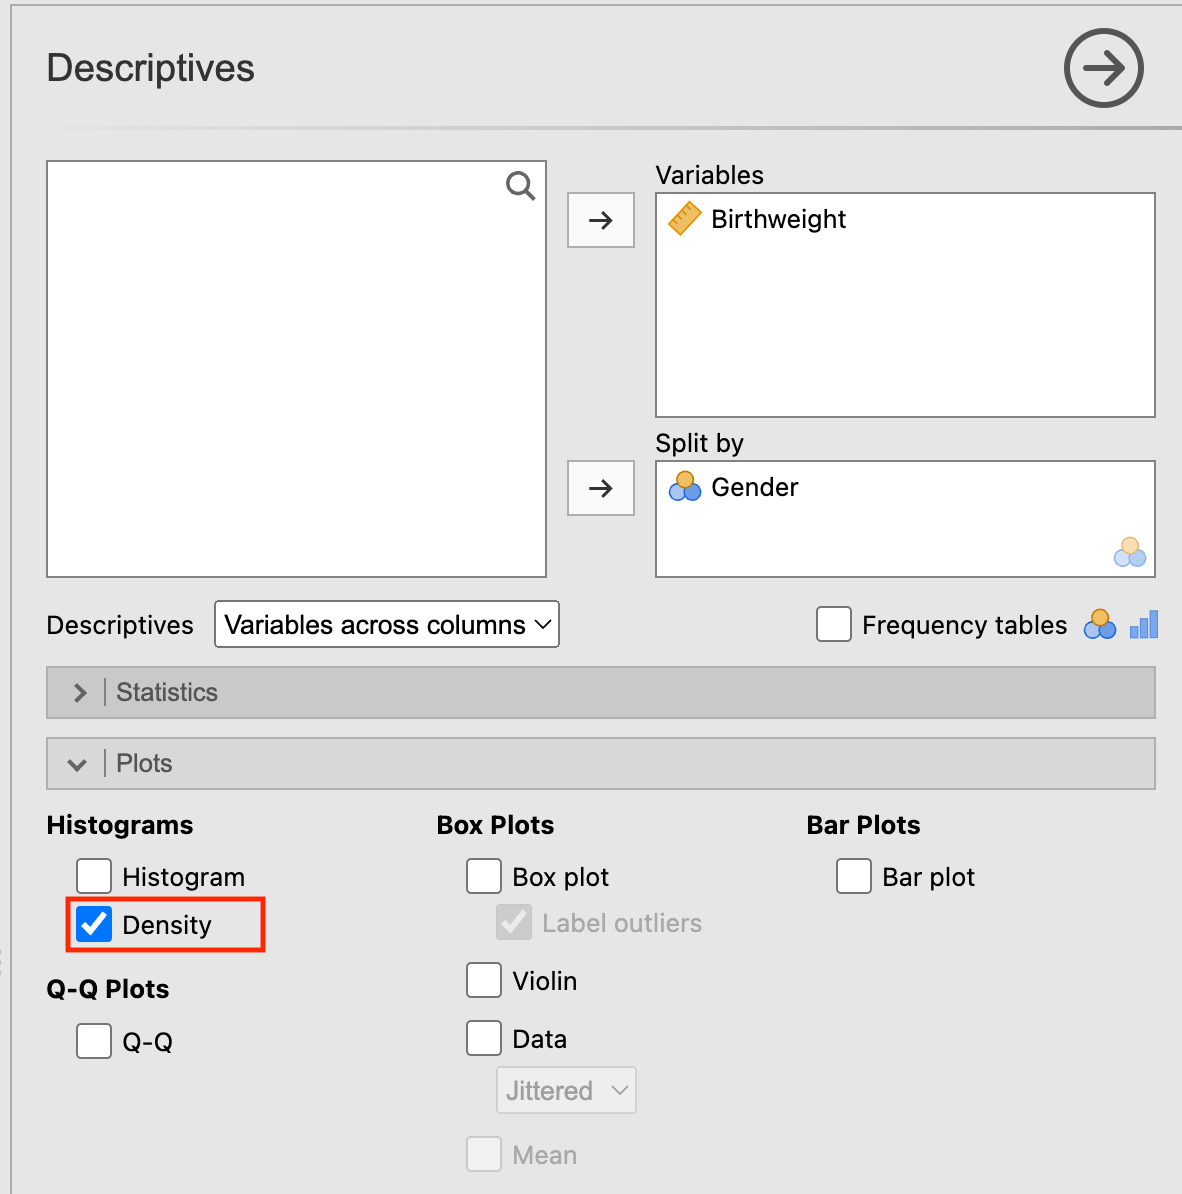
\includegraphics[width=0.66\linewidth,height=\textheight,keepaspectratio]{img/mod05/jamovi/dist-by-1.png}

\section{Independent samples t-test}\label{independent-samples-t-test-1}

To carry out an independent sample t-test, go to \textbf{Analyses
\textgreater{} T-Tests \textgreater{} Independent Samples T-Test}. Move
\texttt{birthweight} into \textbf{Dependent variables} and
\texttt{gender} as the \textbf{Grouping Variable}. Because we don't
assume equal variances of \texttt{birthweight} for males and females, we
tick the \textbf{Welch's} box.

In order to obtain an estimate of the difference in means, with its 95\%
Confidence Interval, tick the relevant boxes in \textbf{Additional
Statistics}:

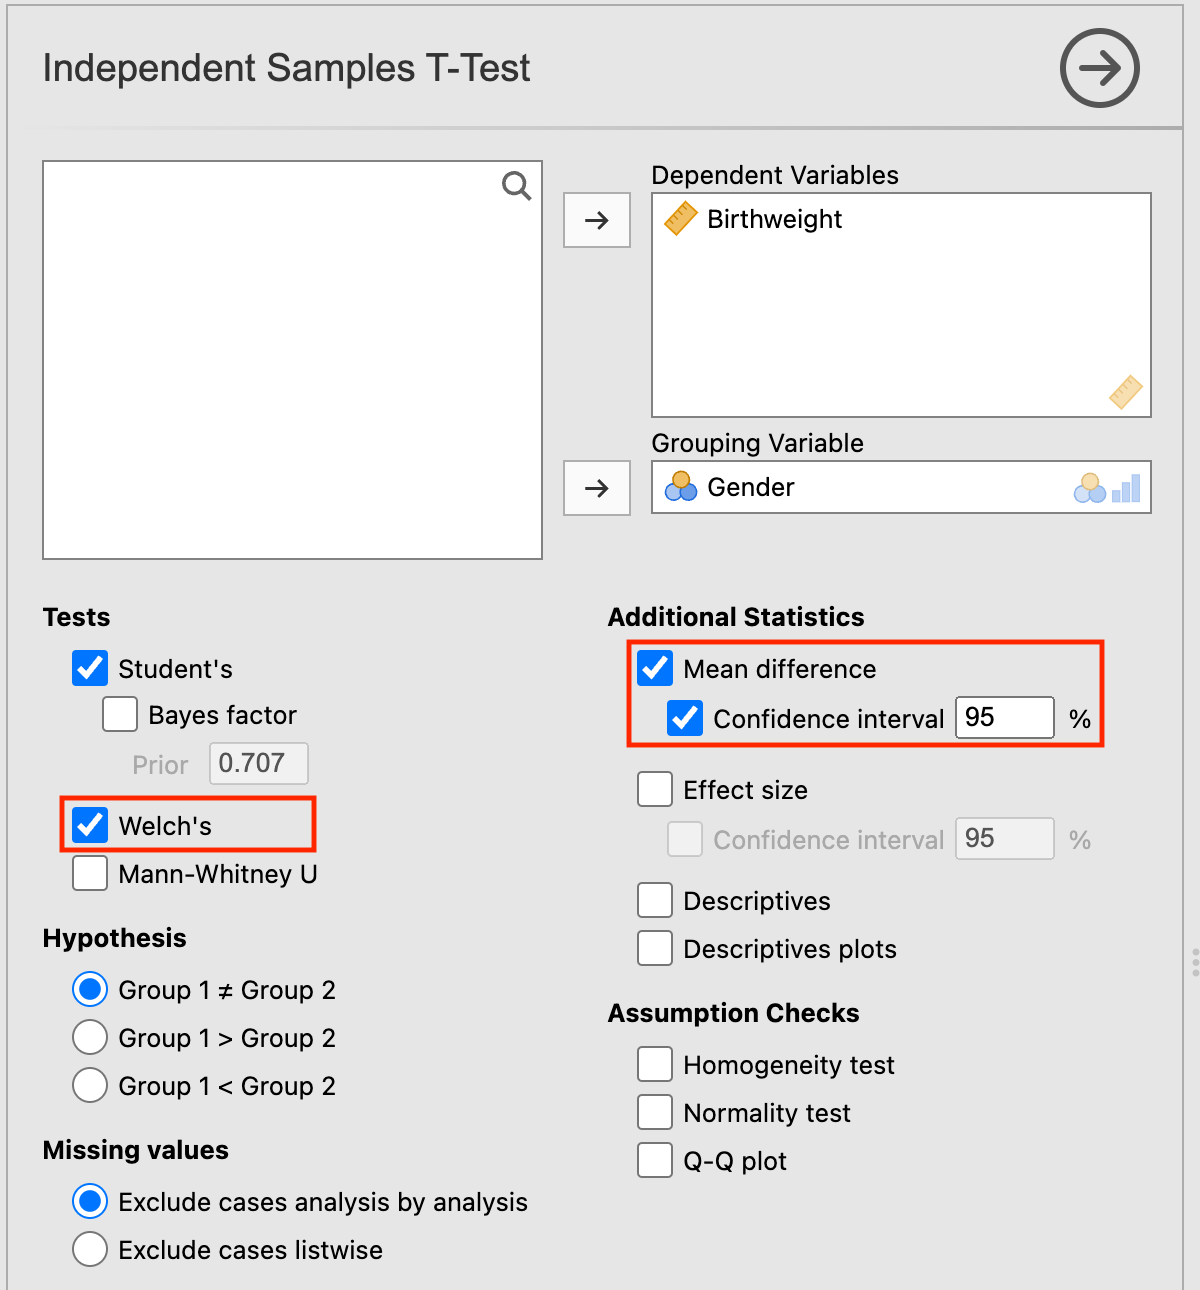
\includegraphics[width=0.66\linewidth,height=\textheight,keepaspectratio]{img/mod05/jamovi/ttest-1-unequal.png}

\section{Checking the assumptions for a Paired
t-test}\label{checking-the-assumptions-for-a-paired-t-test}

Before performing a paired t-test, you must check that the assumptions
for the test have been met. Using the dataset
\texttt{mod05\_ankle\_bp.xlsx} to show that the difference between the
pair of measurements between the sites is normally distributed, we first
need to compute a new variable of the differences.

To create a new column at the end of your dataset, click a cell in the
first empty column, then choose \textbf{Data \textgreater{} Compute}. We
want to compute \texttt{difference} as \texttt{sbp\_dp\ −\ sbp\_tp}, so
we enter this in the formula box as below:

\begin{enumerate}
\def\labelenumi{\arabic{enumi}.}
\tightlist
\item
  Specify the name of the variable to be created: here
  \texttt{difference}
\item
  Click the \emph{f \textsubscript{x}} button to display a list of
  variable names in your dataset
\item
  Double-click the variable \texttt{sbp\_dp} to bring it into the
  formula box
\item
  Type \texttt{-} to represent ``minus''
\item
  Double-click the variable \texttt{sbp\_tp} to bring it into the
  formula box (do not worry if your formula is underlined in red, this
  is simply a spell-check)
\item
  Click the up arrow to close the \textbf{Compute} dialog box
\end{enumerate}

(Note that steps 3 to 5 could also be completed by typing the formula.)

You will see a new column called \texttt{difference} which represents
the difference between the two blood pressures.

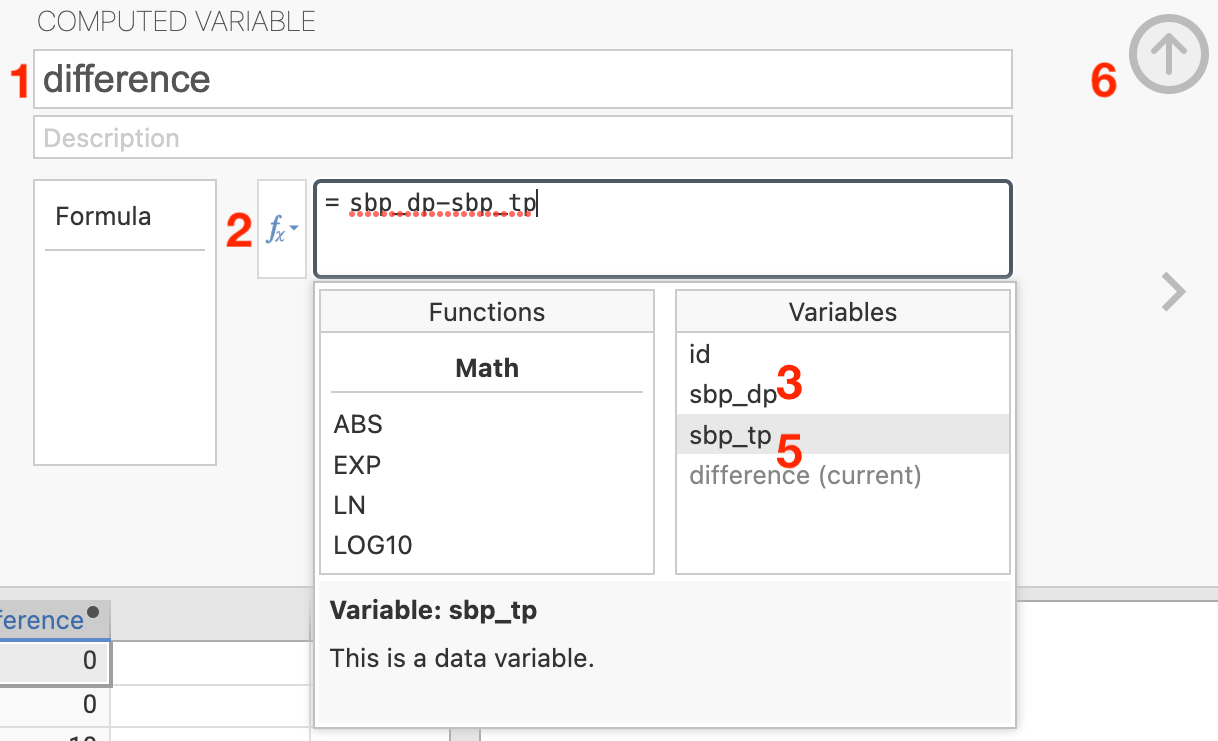
\includegraphics[width=1\linewidth,height=\textheight,keepaspectratio]{img/mod05/jamovi/ttest-paired-1.png}

A density plot of the differences can be constructed in the usual way.

\section{Paired t-Test}\label{paired-t-test}

Using the same blood pressure data as previously, choose
\textbf{Analyses \textgreater{} T-Tests \textgreater{} Paired Samples
T-Test}. Select \texttt{sbp\_dp} and \texttt{sbp\_tp} as the
\textbf{Paired Variables}.

To obtain more informative output, select \textbf{Mean difference} and
\textbf{Confidence interval} as additional statistics. The dialog box
will look like:

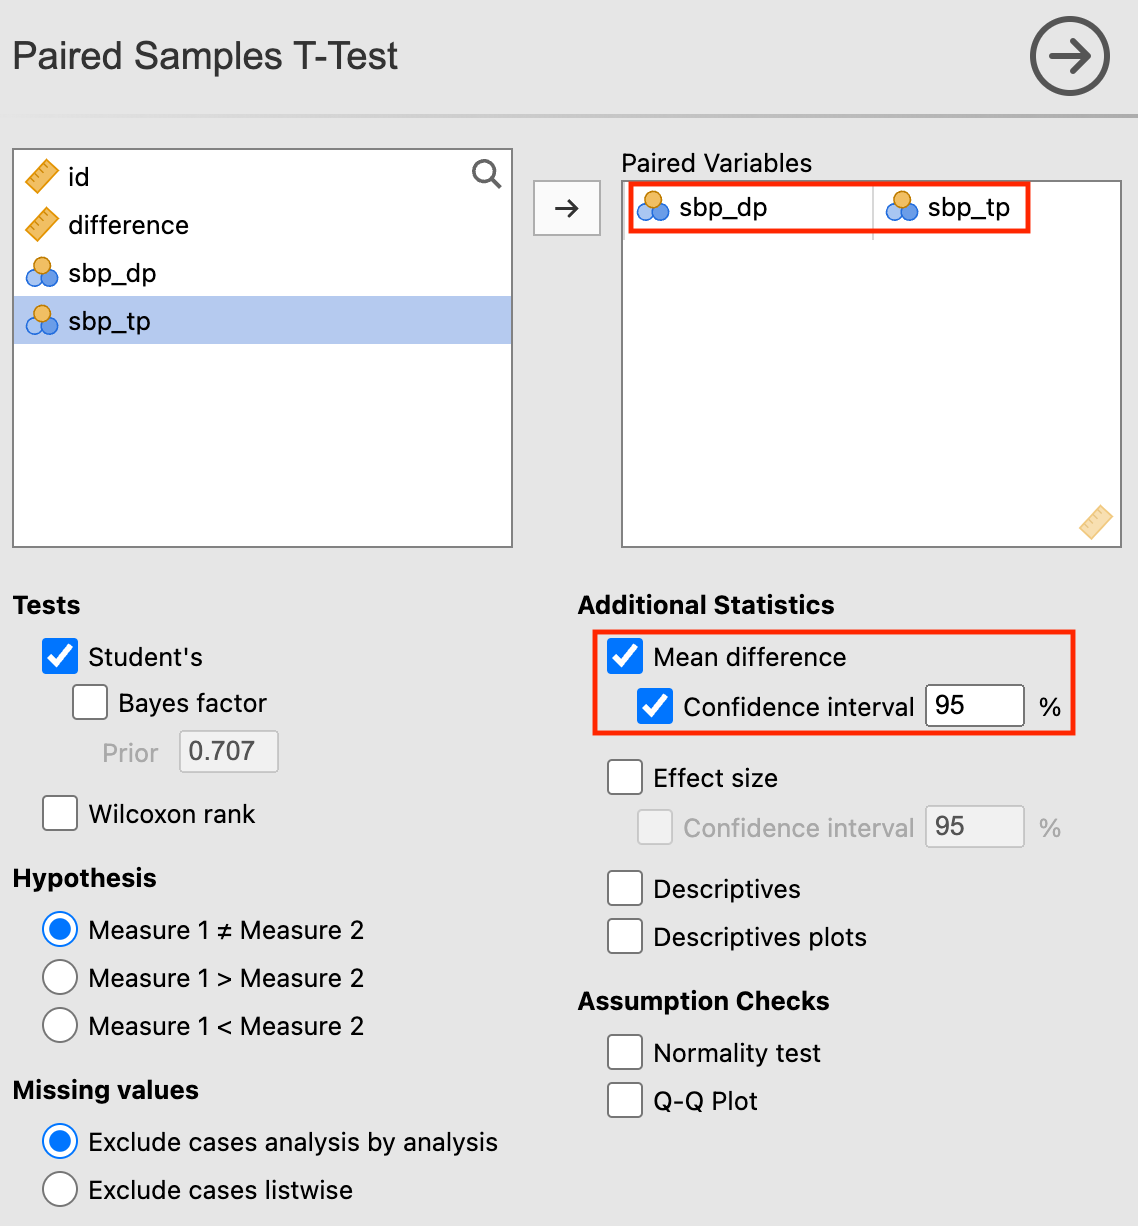
\includegraphics[width=0.66\linewidth,height=\textheight,keepaspectratio]{img/mod05/jamovi/ttest-paired-2.png}

With the following output:

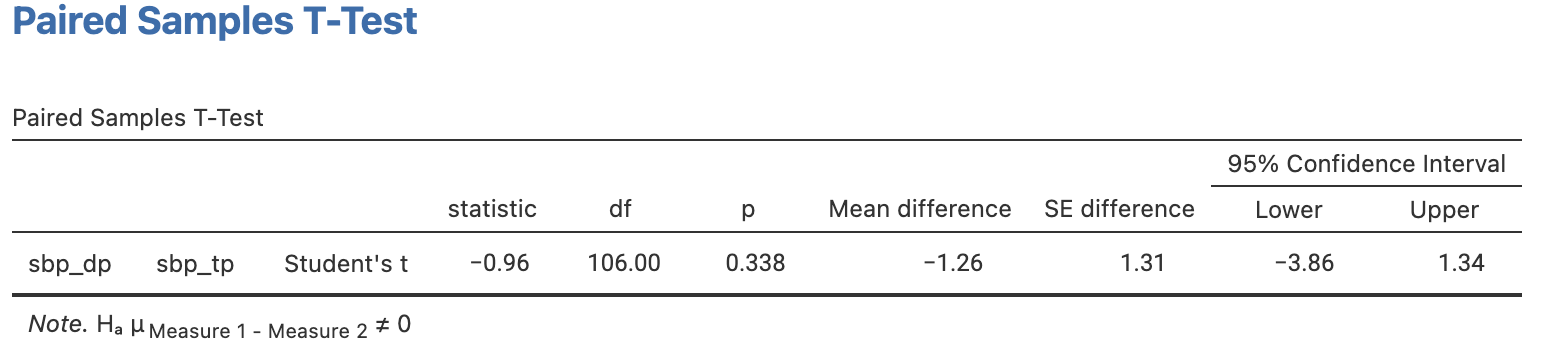
\includegraphics[width=0.66\linewidth,height=\textheight,keepaspectratio]{img/mod05/jamovi/ttest-paired-3.png}

\newpage{}

\bookmarksetup{startatroot}

\chapter*{R notes}\label{r-notes-3}
\addcontentsline{toc}{chapter}{R notes}

\markboth{R notes}{R notes}

\section{Checking data for the independent samples
t-test}\label{checking-data-for-the-independent-samples-t-test-1}

\subsection{Examining variable distributions by a second
variable}\label{examining-variable-distributions-by-a-second-variable-1}

We can use the a \texttt{splitBy} variable in the \texttt{descriptives}
function in the \texttt{jmv} package to obtain summary statistics for
each level of a grouping variable. Further, specifying
\texttt{dens\ =\ TRUE} will produce density plots for the analysis
variable for each level of the grouping variable.

For example, to create the distribution plots in
Figure~\ref{fig-mod05-bwt-gender}, we can use

\begin{Shaded}
\begin{Highlighting}[]
\FunctionTok{library}\NormalTok{(jmv)}

\NormalTok{bwt }\OtherTok{\textless{}{-}} \FunctionTok{readRDS}\NormalTok{(}\StringTok{"data/examples/mod05\_birthweight.rds"}\NormalTok{)}

\FunctionTok{descriptives}\NormalTok{(}\AttributeTok{data =}\NormalTok{ bwt, }\AttributeTok{vars =}\NormalTok{ birthweight, }\AttributeTok{splitBy =}\NormalTok{ gender, }\AttributeTok{dens =} \ConstantTok{TRUE}\NormalTok{)}
\end{Highlighting}
\end{Shaded}

\begin{verbatim}

 DESCRIPTIVES

 Descriptives                                    
 ─────────────────────────────────────────────── 
                         gender    birthweight   
 ─────────────────────────────────────────────── 
   N                     Female             56   
                         Male               44   
   Missing               Female              0   
                         Male                0   
   Mean                  Female       3.587411   
                         Male         3.421364   
   Median                Female       3.530000   
                         Male         3.430000   
   Standard deviation    Female      0.3629788   
                         Male        0.3536165   
   Minimum               Female       2.950000   
                         Male         2.750000   
   Maximum               Female       4.250000   
                         Male         4.100000   
 ─────────────────────────────────────────────── 
\end{verbatim}

\pandocbounded{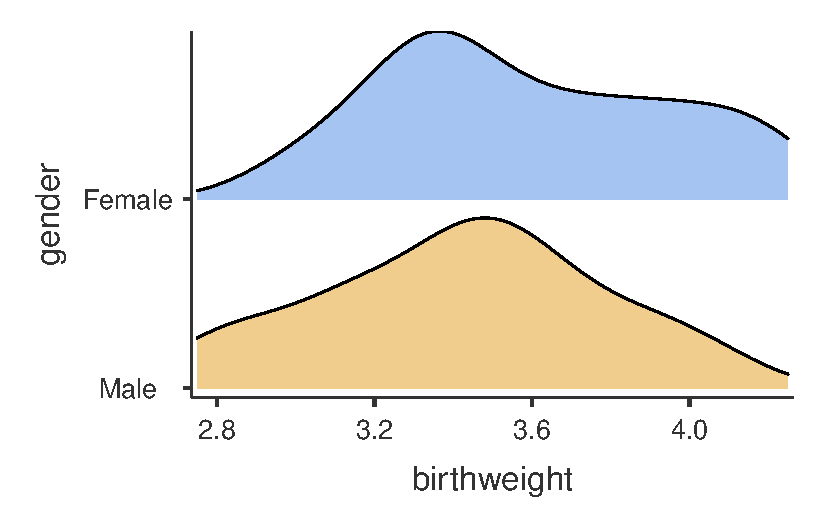
\includegraphics[keepaspectratio]{05-comparing-two-means_files/figure-pdf/unnamed-chunk-2-1.pdf}}

Of course, we could also use \texttt{ggplot2} to produce the density
plots, defining \texttt{gender} as a \texttt{facet\_wrap}:

\begin{Shaded}
\begin{Highlighting}[]
\FunctionTok{library}\NormalTok{(ggplot2)}

\FunctionTok{ggplot}\NormalTok{(}\AttributeTok{data=}\NormalTok{bwt, }\FunctionTok{aes}\NormalTok{(}\AttributeTok{x=}\NormalTok{birthweight)) }\SpecialCharTok{+}
  \FunctionTok{geom\_density}\NormalTok{() }\SpecialCharTok{+}
  \FunctionTok{facet\_wrap}\NormalTok{(}\FunctionTok{vars}\NormalTok{(gender)) }\SpecialCharTok{+}
  \FunctionTok{theme\_classic}\NormalTok{() }\SpecialCharTok{+}
  \FunctionTok{labs}\NormalTok{(}\AttributeTok{x=}\StringTok{"Birthweight (kg)"}\NormalTok{)}
\end{Highlighting}
\end{Shaded}

\pandocbounded{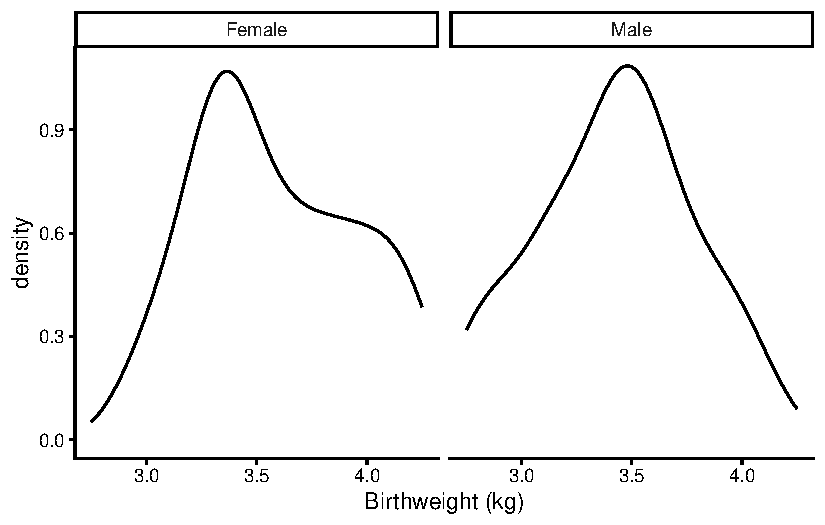
\includegraphics[keepaspectratio]{05-comparing-two-means_files/figure-pdf/unnamed-chunk-3-1.pdf}}

\section{Independent samples t-test}\label{independent-samples-t-test-2}

We can use the \texttt{ttestIS()} (t-test, independent samples) function
from the \texttt{jmv} package to perform the independent samples t-test.
We include the \texttt{meanDiff=TRUE} and \texttt{ci=TRUE} options to
obtain the difference in means, with its 95\% confidence interval. We
can request a Welch's test (which does not assume equal variances) by
the \texttt{welchs=TRUE} option (note that output has been edited to fit
on the page):

\begin{verbatim}
ttestIS(data = bwt, vars = birthweight, group = gender, 
        meanDiff = TRUE, ci = TRUE, welchs = TRUE)


INDEPENDENT SAMPLES T-TEST

 Independent Samples T-Test                                                                                                          
─────────────────────────────────────────────────────────────────────
                                 Statistic    df          p           
─────────────────────────────────────────────────────────────────────
   birthweight    Student's t     2.296556    98.00000    0.0237731   
                  Welch's t       2.303840    93.54377    0.0234458   
─────────────────────────────────────────────────────────────────────
────────────────────────────────────────────────────────────────────────────── 
                Mean difference    SE difference    Lower         Upper       
────────────────────────────────────────────────────────────────────────────── 
  Student's t        0.1660471       0.07230265    0.02256481    0.3095293   
  Welch's t          0.1660471       0.07207403    0.02293328    0.3091609   
────────────────────────────────────────────────────────────────────────────── 
   Note. Hₐ μ <sub>Female</sub> ≠ μ <sub>Male</sub>
\end{verbatim}

\section{Checking the assumptions for a Paired
t-test}\label{checking-the-assumptions-for-a-paired-t-test-1}

Before performing a paired t-test, you must check that the assumptions
for the test have been met. Using the dataset
\texttt{mod05\_ankle\_bp.xlsx} to show that the difference between the
pair of measurements between the sites is normally distributed, we first
need to compute a new variable of the differences and examine its
distribution.

\begin{Shaded}
\begin{Highlighting}[]
\FunctionTok{library}\NormalTok{(readxl)}
\FunctionTok{library}\NormalTok{(dplyr)}

\NormalTok{sbp }\OtherTok{\textless{}{-}} \FunctionTok{read\_excel}\NormalTok{(}\StringTok{"data/examples/mod05\_ankle\_bp.xlsx"}\NormalTok{) }\SpecialCharTok{|\textgreater{}} 
  \FunctionTok{mutate}\NormalTok{(}\AttributeTok{diff =}\NormalTok{ sbp\_dp }\SpecialCharTok{{-}}\NormalTok{ sbp\_tp)}

\FunctionTok{descriptives}\NormalTok{(}\AttributeTok{data =}\NormalTok{ sbp, }\AttributeTok{vars =}\NormalTok{ diff, }\AttributeTok{dens =} \ConstantTok{TRUE}\NormalTok{)}
\end{Highlighting}
\end{Shaded}

\begin{verbatim}

 DESCRIPTIVES

 Descriptives                        
 ─────────────────────────────────── 
                         diff        
 ─────────────────────────────────── 
   N                           107   
   Missing                       0   
   Mean                  -1.261682   
   Median                 0.000000   
   Standard deviation     13.56489   
   Minimum               -40.00000   
   Maximum                65.00000   
 ─────────────────────────────────── 
\end{verbatim}

\pandocbounded{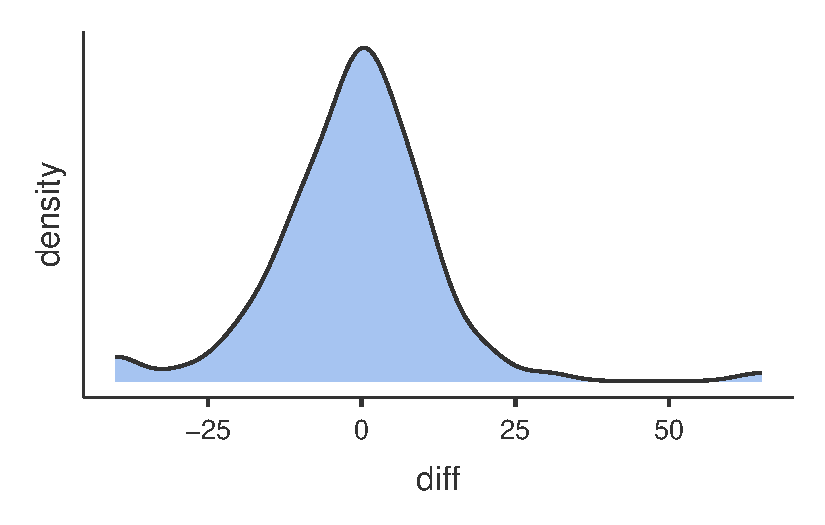
\includegraphics[keepaspectratio]{05-comparing-two-means_files/figure-pdf/unnamed-chunk-4-1.pdf}}

While there is a large difference in blood pressure (around 60 mmHg)
that warrants further checking, the curve is roughly symmetric with an
approximately Normal distribution.

\section{Paired t-Test}\label{paired-t-test-1}

To perform a paired t-test we will use the dataset
\texttt{mod05\_ankle\_bp.xlsx}. We can perform a paired t-test using the
\texttt{ttestPS()} function within the \texttt{jmv} package, where we
defined the paired observations as: `pairs=list(list(i1 = `variable1',
i2 = `variable2'))

\begin{verbatim}
ttestPS(data = sbp, pairs = list(list(i1 = "sbp_dp", i2 = "sbp_tp")),
        meanDiff = TRUE, ci = TRUE)
        

 PAIRED SAMPLES T-TEST

 Paired Samples T-Test                                                                                                                   
 ──────────────────────────────────────────────────────────────────────────
                                      statistic     df          p          
 ──────────────────────────────────────────────────────────────────────────
   sbp_dp    sbp_tp    Student's t    -0.9621117    106.0000    0.3381832  
 ──────────────────────────────────────────────────────────────────────────
 ────────────────────────────────────────────────────────────────────────────── 
                        Mean difference    SE difference    Lower        Upper      
 ────────────────────────────────────────────────────────────────────────────── 
   sbp_dp    sbp_tp        -1.261682         1.311368    -3.861596    1.338232   
 ────────────────────────────────────────────────────────────────────────────── 
   Note. Hₐ μ <sub>Measure 1 - Measure 2</sub> ≠ 0
\end{verbatim}

The syntax of the ttestPS function is a little cumbersome. The
\texttt{t.test} function can be used as an alternative:

\begin{Shaded}
\begin{Highlighting}[]
\FunctionTok{t.test}\NormalTok{(sbp}\SpecialCharTok{$}\NormalTok{sbp\_dp, sbp}\SpecialCharTok{$}\NormalTok{sbp\_tp, }\AttributeTok{paired =} \ConstantTok{TRUE}\NormalTok{)}
\end{Highlighting}
\end{Shaded}

\begin{verbatim}

    Paired t-test

data:  sbp$sbp_dp and sbp$sbp_tp
t = -0.96211, df = 106, p-value = 0.3382
alternative hypothesis: true mean difference is not equal to 0
95 percent confidence interval:
 -3.861596  1.338232
sample estimates:
mean difference 
      -1.261682 
\end{verbatim}

\newpage{}

\bookmarksetup{startatroot}

\chapter*{Activities}\label{activities-4}
\addcontentsline{toc}{chapter}{Activities}

\markboth{Activities}{Activities}

\subsection*{Activity 5.1}\label{activity-5.1}
\addcontentsline{toc}{subsection}{Activity 5.1}

Indicate what type of t-test could be used to analyse the data from the
following studies and provide reasons:

\begin{enumerate}
\def\labelenumi{\alph{enumi})}
\tightlist
\item
  A total of 60 university students are randomly assigned to undergo
  either cognitive behavioural therapy or mindfulness therapy to improve
  their mental health. After ten therapeutic sessions, each student's
  anxiety is assessed via a mental health questionnaire.
\item
  A researcher wishes to determine whether attendance at a day care
  centre increases the scores of three year old twins on a motor skills
  test. Random assignment is used to decide which member from each of 30
  pairs of twins attends the day care centre and which member stays at
  home.
\item
  A child psychologist assigns aggression scores to each of 10 children
  during two 60 minute observation periods separated by an intervening
  exposure to a series of violent TV cartoons.
\item
  A marketing researcher measures 100 doctors' reports of the number of
  their patients asking them about a particular drug during the month
  before and the month after a major advertising campaign.
\end{enumerate}

\subsection*{Activity 5.2}\label{activity-5.2}
\addcontentsline{toc}{subsection}{Activity 5.2}

A study was conducted to compare haemoglobin levels in the blood of
children with and without cystic fibrosis. It is known that haemoglobin
levels are normally distributed in children. The data are stored in
Activity\_5.2.csv as:

\begin{itemize}
\tightlist
\item
  cf: cystic fibrosis: 0=no, 1=yes
\item
  haem: haemoglobin (g/dL)
\end{itemize}

Analyse these data to address the research question.

\subsection*{Activity 5.3}\label{activity-5.3}
\addcontentsline{toc}{subsection}{Activity 5.3}

A randomised controlled trial (RCT) was carried out to investigate the
effect of a new supplement in increasing the hematocrit (\%) value in
anaemic participants. In the study, hematocrit was measured as the
proportion of blood that is made up of red blood cells. Hematocrit
levels are often lower in anaemic people who do not have sufficient
healthy red blood cells. In the RCT, 33 people in the intervention group
received the new supplement and 31 people in the control group received
standard care (i.e.~the usual supplement was given). After 4 weeks,
hematocrit values were measured as entered in the file
\texttt{Activity\_5.3.rds}. In the community, hematocrit levels are
normally distributed.

Analyse these data to address the research question.

\subsection*{Activity 5.4}\label{activity-5.4}
\addcontentsline{toc}{subsection}{Activity 5.4}

A total of 41 babies aged 6 months to 2 years with haemangioma (birth
mark) were enrolled in a study to test the effect of a new topical
medication in reducing the volume of their haemangioma. Parents were
asked to apply the medication twice daily. The volume (in mm3) of the
haemangioma was measured at enrolment and again after 12 weeks of using
the medication. The data are saved in \texttt{Activity\_5.4.rds}.

Analyse these data to answer the research question. Are there any
limitations of this study?

\subsection*{Supplementary Activity
5.5}\label{supplementary-activity-5.5}
\addcontentsline{toc}{subsection}{Supplementary Activity 5.5}

A study was conducted to investigate cardiovascular health of
Australians. In this study heart rates were recorded by a heart rate
monitor on each participant following 30 minutes of intense aerobic
exercise. The researchers are interested in whether there is a
difference in the mean post-exercise heart rates of females aged 20 --
24 years compared to females aged 25 -- 30 years.

A dataset containing the study information is provided in the file
\texttt{Activity\_5.5\_heartrate.csv}. There are 149 observations in the
dataset with the following variables:

\begin{itemize}
\tightlist
\item
  id: id number
\item
  agegroup: age range of the females (1 = 20 -- 24 years; 2 = 25 -- 30
  years)
\item
  heartrate: heart rate (beats/minute)
\end{itemize}

Analyse these data to answer the research question.

\subsection{Supplementary Activity
5.6}\label{supplementary-activity-5.6}

A study was conducted to assess the effectiveness of a health promotion
program to improve the fitness of school children. The fitness of 58
children from an inner-city school was assessed by measuring the total
distance each child could run in a 10-minute period.

The following data are stored in \texttt{Activity\_5.6\_fitness.csv}:

\begin{itemize}
\tightlist
\item
  id: participant ID
\item
  before: 10-minute running distance before the program (metres)
\item
  after: 10-minute running distance after the program (metres)
\end{itemize}

Analyse these data to answer the research question.

\bookmarksetup{startatroot}

\chapter{Summary statistics for binary
data}\label{summary-statistics-for-binary-data}

\section*{Learning objectives}\label{learning-objectives-5}
\addcontentsline{toc}{section}{Learning objectives}

\markright{Learning objectives}

By the end of this module you will be able to:

\begin{itemize}
\tightlist
\item
  Compute and interpret 95\% confidence intervals for proportions;
\item
  Conduct and interpret a significance test for a one-sample proportion;
\item
  Use statistical software to compute 95\% confidence intervals for a
  difference in proportions, a relative risk and an odds ratio.
\end{itemize}

\section*{Optional readings}\label{optional-readings-5}
\addcontentsline{toc}{section}{Optional readings}

\markright{Optional readings}

Kirkwood and Sterne (2001); Chapter 16
\href{http://er1.library.unsw.edu.au/er/cgi-bin/eraccess.cgi?url=https://ebookcentral.proquest.com/lib/unsw/detail.action?docID=624728}{{[}UNSW
Library Link{]}}

Bland (2015); Section 8.6, Section 13.7
\href{http://er1.library.unsw.edu.au/er/cgi-bin/eraccess.cgi?url=https://ebookcentral.proquest.com/lib/unsw/detail.action?docID=5891730}{{[}UNSW
Library Link{]}}

\section{Introduction}\label{introduction-5}

In Modules 4 and 5, we discussed methods used to analyse continuous
data. In Modules 6 and 7, we will focus on analysing categorical data.

In health research, we often collect information that can be classified
into two categories, e.g.~male and female, disease present or disease
absent etc. Binary categorical variables such as these are summarised
using proportions.

\section{Calculating proportions and 95\% confidence
intervals}\label{calculating-proportions-and-95-confidence-intervals}

\subsection{Calculating a proportion}\label{calculating-a-proportion}

We need two pieces of information to calculate a proportion: \(n\), the
total number of observations, and \(k\), the number of `successes'. Note
that we use the term `success' to describe the outcome of interest,
recognising that a success may be a adverse outcome such as death or
disease.

The following formula is used to calculate the proportion, \(p\):

\[ p = k / n \]

The proportion, \(p\), is a number that lies between 0 and 1.
Proportions and their confidence intervals can easily be converted to
percentages by multiplying by 100 once computed.

As for all summary statistics, it is useful to compute the precision of
the estimate as a 95\% confidence interval (CI) to indicate the range of
values in which are 95\% confident that the true population value lies.
In this module, we present two methods for computing a 95\% confidence
interval around a proportion.

\subsection{Calculating the 95\% confidence interval of a proportion
(Wald
method)}\label{calculating-the-95-confidence-interval-of-a-proportion-wald-method}

The Wald method for calculating the 95\% confidence interval is based on
assuming that the proportion, \(p\), is Normally distributed. This
assumption is reasonable if the sample is sufficiently large (for
example, if \(n>30\)) and if \(n \times (1-p)\) and \(n \times p\) are
both larger than 5.

The Wald method for calculating a 95\% confidence interval is given by:

\[\text{95\% CI} = p \pm (1.96 \times \text{SE}(p))\]

where the standard error of a proportion is computed as:

\[\text{SE}(p) = \sqrt{\frac{p \times (1 - p)}{n}}\]

\subsection{Worked Example 6.1}\label{worked-example-6.1}

In a cross-sectional study of children living in a rural village, 47
children from a random sample of 215 children were found to have
scabies. Here \(n=215\) and \(k=47\), so the proportion of children with
scabies is estimated as:

\[ p = \frac{47}{215} = 0.2186 \]

Given the large sample size and the number of children with the rarer
outcome is larger than 5, the Wald method is used to calculate the
standard error of the proportion as:

\[{\text{SE}\left( p \right) = \sqrt{\frac{0.2186 \times (1 - 0.2186)}{215}}
}{= 0.02819}\]

Then, the 95\% confidence interval is estimated as:

\[\text{95\% CI} = 0.2186 \pm 1.96 \times 0.02819\]

\[= 0.1634 \text{ to } 0.2739\]

The prevalence of scabies among children in the village is 21.9\% (95\%
CI 16.3\%, 27.4\%). These values tell us that we are 95\% confident that
the true prevalence of scabies among children in the village is between
16.3\% and 27.4\%.

\subsection{Calculating the 95\% confidence interval of a proportion
(Wilson
method)}\label{calculating-the-95-confidence-interval-of-a-proportion-wilson-method}

Another method to calculate the confidence interval of a proportion is
the Wilson (sometimes also called the `score') method. We can use it in
situations where it is not appropriate to use the normal approximation
to the binomial distribution as described above i.e.~if the sample size
is small (\(n < 30\)) or the number of observations with the rarer
outcome is 5 or fewer. This method much more difficult to implement by
hand than the standard confidence interval, and so we will not discuss
the hand calculation using the mathematical equation in this course.
Instead, we use statistical software to do this (see the jamovi or R
notes for detail).

When using software, our worked example provides a 95\% confidence
interval of the prevalence of scabies of 16.9\% to 27.9\%.

\subsection{Wald vs Wilson methods}\label{wald-vs-wilson-methods}

The Wald method, which assumes that the underlying proportion follows a
Normal distribution, is easy to calculate and follows the form of other
confidence intervals. The Wilson method, which is difficult to calculate
by hand, has nicer mathematical properties. There are also a number of
other methods for calculating confidence intervals for proportions, but
we do not discuss these in this course.

A paper by Brown, Cai and DasGupta (Brown et al. (2001)) has compared
the properties of the Wald and Wilson methods (among others) and
concluded that the Wilson method is preferred over the Wald method.
\textbf{Therefore, we recommend the Wilson method be used to calculate
95\% confidence intervals for a proportion.} Note that it is not
possible to compute a Wilson confidence interval using jamovi. The
interval calculated by jamovi is the Clopper-Pearson interval.

\section{Hypothesis testing for one sample
proportion}\label{hypothesis-testing-for-one-sample-proportion}

We can carry out a hypothesis test to compare a sample proportion to a
hypothesised proportion. In much the same way as a one sample t-test was
used in Module 5 to test a sample mean against a hypothesised mean, we
can perform a one-sample test to test a sample proportion against a
hypothesised proportion. The significance test will provide a P-value to
assess the evidence against the null hypothesis, while the 95\%
confidence interval will provide the range in which we are 95\%
confident that the true proportion lies.

For example, we can test the following null hypothesis:

H\textsubscript{0}: sample proportion is not different from the
hypothesised proportion

Much like constructing a 95\% confidence interval, there are two main
options when performing a hypothesis test on a single proportion: the
first assumes that the proportion follows a Normal distribution, while
the second relaxes this assumption.

\subsection{z-test for testing one sample
proportion}\label{z-test-for-testing-one-sample-proportion}

The first step in the z-test is to calculate a z-statistic, which is
then used to calculate a P-value. The z-statistic is calculated as the
difference between the population proportion and the sample proportion
divided by the standard error of the population proportion, i.e.

\[
z = \frac{(p_{sample} - p_{population})}{\text{SE}(p_{population})}
\]

This z-statistic is then compared to the standard Normal distribution to
calculate the P-value.

\subsection{Worked Example 6.2}\label{z-prop-example}

A national census in a country shows that 20\% of the population are
smokers. A survey of a community within the country that has received a
public health anti-smoking intervention shows that 54 of 300 people
sampled are smokers (18\%). We can calculate a 95\% confidence interval
around this proportion using the Wilson method, which is calculated as
14.1\% to 22.7\%.

The researchers are interested in whether the proportion of smoking in
this community is the same as the population prevalence of smoking of
20\%. The null hypothesis can be written as: H\textsubscript{0}: the
proportion of smokers in the community is 20\% (the same as in the
national census).

We can test this by calculating a z-statistic:

\[
\begin{aligned}
z &= \frac{(0.18 - 0.20)}{\sqrt{\frac{0.20 × (1 - 0.20)}{300}}} \\
 &= -0.87
\end{aligned}
\]

The P-value for the test above can be obtained from a Normal
distribution table as \(P = 2 × 0.192 = 0.38\) (using statistical
software). This indicates that there is insufficient evidence to
conclude that there is a difference between the proportion of smokers in
the community and the country. This is consistent with our 95\%
confidence interval which crosses the null value of 20\%.

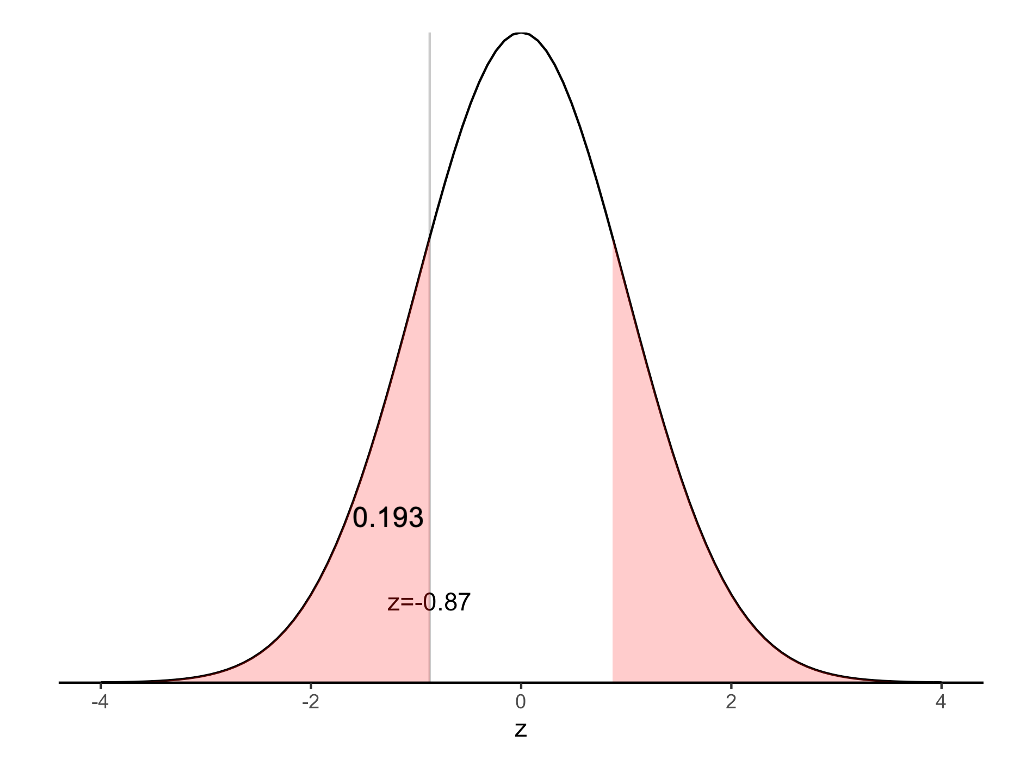
\includegraphics[width=0.66\linewidth,height=\textheight,keepaspectratio]{img/mod06/z-curve.png}

\subsection{Binomial test for testing one sample
proportion}\label{binomial-test-for-testing-one-sample-proportion}

We can use the binomial distribution to obtain an exact P-value for
testing a single proportion. Historically, this was a time consuming
process with much hand calculation. These days, statistical software
performs the calculations quickly and efficiently, and is the preferred
method.

\subsection{Worked example 6.3}\label{worked-example-6.3}

The file \texttt{mod06\_smoking\_status.rds} contains the data for this
example. In the data file, smokers are coded as 1 and non-smokers are
coded as 0. In jamovi, we can perform the binomial test, while in R, we
can use the \texttt{prop.test} function to perform a z-test, or the
\texttt{binom.test} function to perform the binomial test.

The z-test provides a two-sided P-value of 0.39, while the binomial test
gives a two-sided P-value of 0.43. Both tests provide little evidence
against the hypothesis that the prevalence of smoking in the community
is 20\%.

\section{Contingency tables}\label{contingency-tables}

As introduced in PHCM9794: Foundations of Epidemiology, 2-by-2
contingency tables can be used to examine associations between two
binary variables, most commonly an exposure and an outcome. The
traditional form of a 2-by-2 contingency table is given in
Table~\ref{tbl-2-by-2-trad}.

\begin{table}[h]

\caption{\label{tbl-2-by-2-trad}Traditional format for presenting a
contingency table}

\centering{

\centering
\begin{tblr}[         %% tabularray outer open
]                     %% tabularray outer close
{                     %% tabularray inner open
colspec={Q[]Q[]Q[]Q[]},
hline{2}={1-4}{solid, black, 0.05em},
hline{1}={1-4}{solid, black, 0.08em},
hline{5}={1-4}{solid, black, 0.08em},
}                     %% tabularray inner close
& Outcome present & Outcome absent & Total \\
Exposure present & a & b & a+b \\
Exposure absent & c & d & c+d \\
Total & a+c & b+d & N \\
\end{tblr}

}

\end{table}%

When using a statistics program, it is recommended that the outcome and
exposure variables are coded by assigning `absent' as 0 and `present' as
1, for example `No' = 0 and `Yes' = 1. This coding ensures that measures
of association, such as the odds ratio or relative risk, are computed
correctly. While R does not strictly require this coding to be followed,
it is good practice nonetheless.

\section{A brief summary of epidemiological study
types}\label{a-brief-summary-of-epidemiological-study-types}

In this section, we wil present a very brief summary of three study
types commonly used in population health research. This topic is covered
in much more detail in \textbf{PHCM9794: Foundations of Epidemiology},
and more detail can be found in Chapter 4 of Essential Epidemiology (3rd
or 4th edition) Webb, Bain and Page (Webb et al. (2016)).

\subsection{Randomised controlled
trial}\label{randomised-controlled-trial}

A randomised controlled trial addresses the research question: what is
the effect of an intervention on an outcome. In the simplest form of a
randomised controlled trial, a group of participants is randomly
allocated to a group that receives the treatment of interest or to a
control group that does not receive the treatment of interest.
Participants are followed up over time, and the outcome is measured at
the conclusion of the study.

\begin{figure}[H]

{\centering 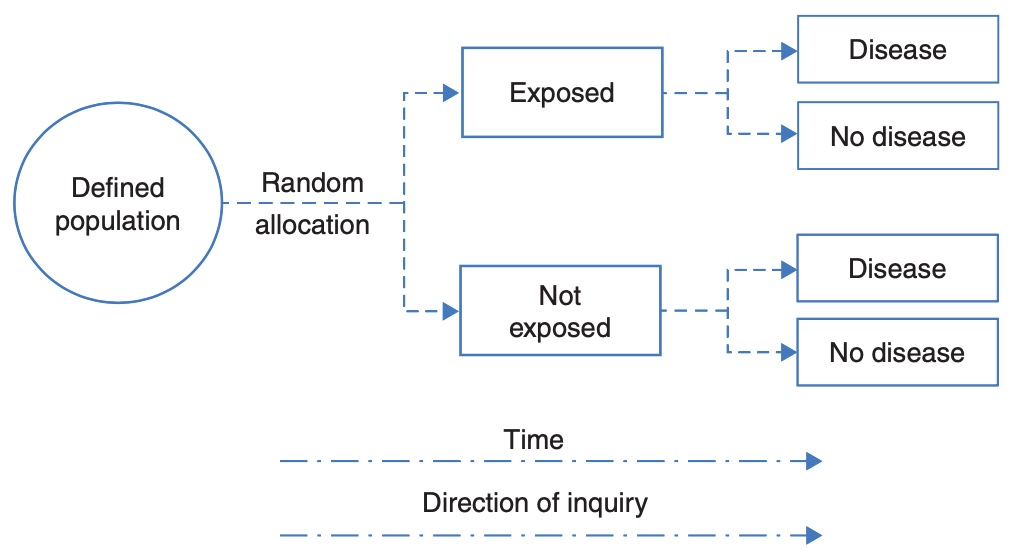
\includegraphics[width=0.66\linewidth,height=\textheight,keepaspectratio]{img/mod06/ee-rct.jpg}

}

\caption{The design of a randomised controlled trial {[}Figure 4.1,
Essential Epidemiology{]}}

\end{figure}%

\subsection{Cohort study}\label{cohort-study}

A cohort study is an \emph{observational study} that addresses the
research question: what is the effect of an exposure on an outcome. This
research question is similar to that studied in a randomised controlled
trial, but the exposure is defined by the participants' circumstances,
and not manipulated by the researchers. In a cohort study, participants
without the outcome of interest are enrolled, followed over time, and
information on their exposure to a factor is measured (either at
baseline or over time). At the conclusion of the study, information on
the outcome is measured to identify new (incident) cases.

\begin{figure}[H]

{\centering 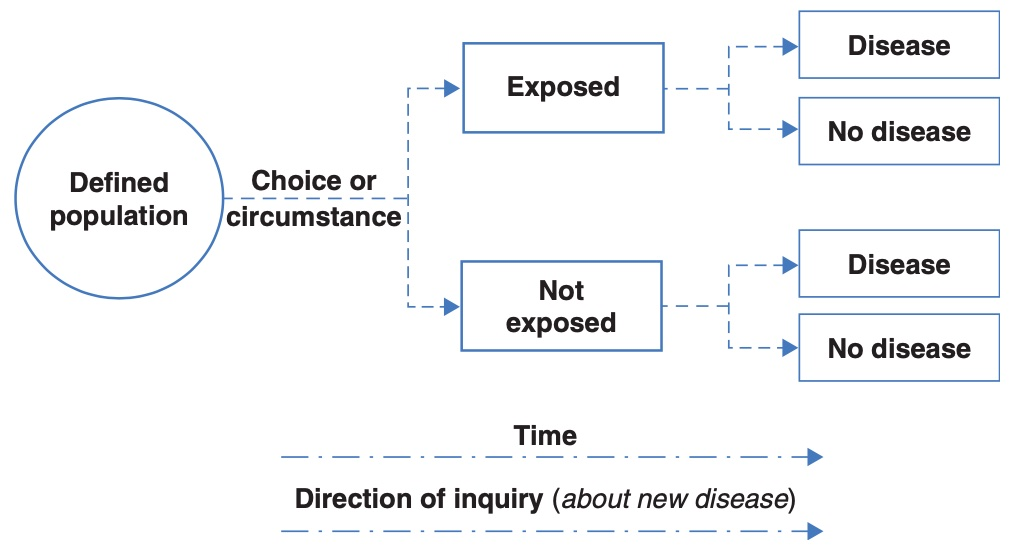
\includegraphics[width=0.66\linewidth,height=\textheight,keepaspectratio]{img/mod06/ee-cohort.jpg}

}

\caption{The design of a cohort study {[}Figure 4.2, Essential
Epidemiology{]}}

\end{figure}%

\subsection{Case control study}\label{case-control-study}

While the randomised controlled trial and cohort study begin with a
population without the outcome, a case-control study begins by
assembling a group with the outcome of interest (cases), and a group
without the outcome of interest (controls). The researchers then ask the
cases and controls about their previous exposures.

\begin{figure}[H]

{\centering 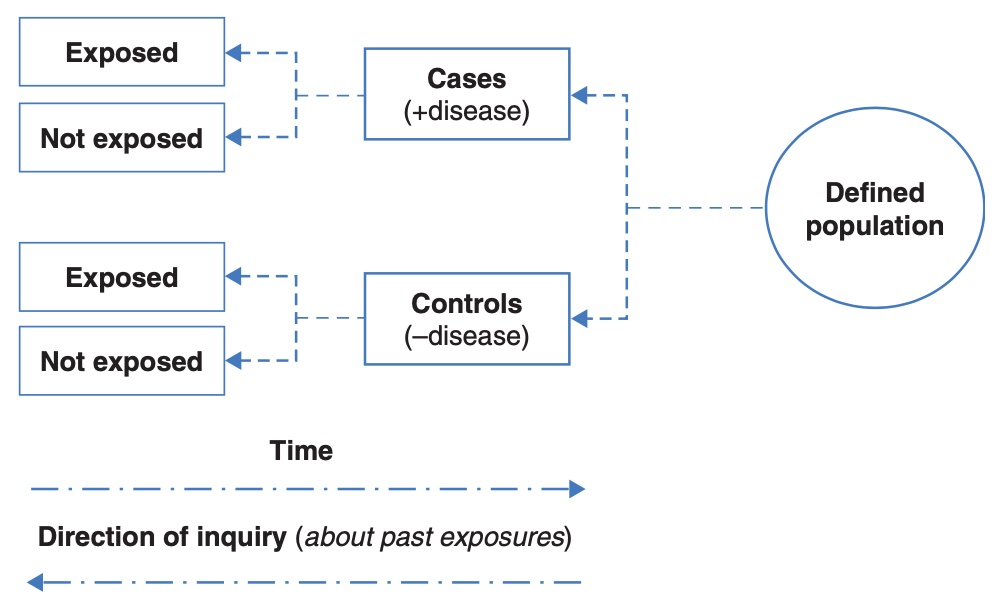
\includegraphics[width=0.66\linewidth,height=\textheight,keepaspectratio]{img/mod06/ee-cc.jpg}

}

\caption{The design of a case-control trial {[}Figure 4.3, Essential
Epidemiology{]}}

\end{figure}%

\subsection{Cross-sectional study}\label{cross-sectional-study}

In a cross-sectional study, the exposure and the outcome are measured at
the same time. While this results in a study that is relatively quick to
conduct, it does not allow for any temporal relationships to be
assessed.

\begin{figure}[H]

{\centering 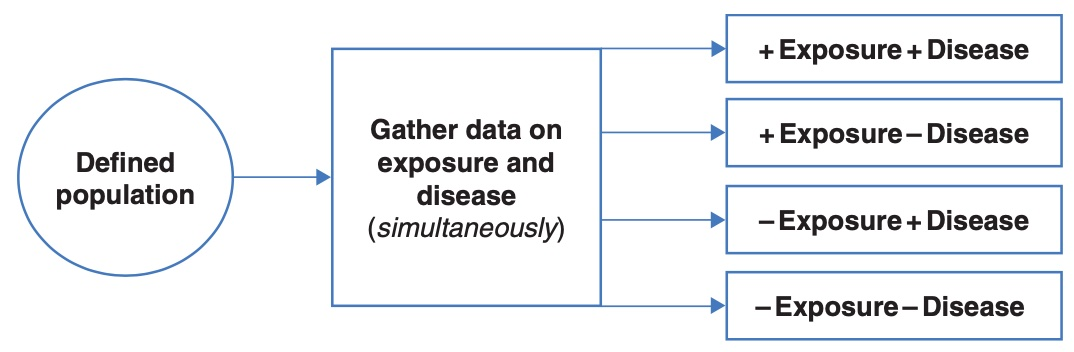
\includegraphics[width=0.66\linewidth,height=\textheight,keepaspectratio]{img/mod06/ee-cs.jpg}

}

\caption{The design of a cross-sectional study {[}Figure 4.4, Essential
Epidemiology{]}}

\end{figure}%

\section{Measures of effect for epidemiological
studies}\label{measures-of-effect-for-epidemiological-studies}

We can calculate a \textbf{relative} measure of association between an
exposure and an outcome as either a relative risk or odds ratio. The
relative risk is a direct comparison of the risk in the exposed group
with the risk in the non-exposed group, and can only be calculated for a
cohort study (including a randomised controlled trial) or a
cross-sectional study (where it is also called a \emph{prevalence
ratio}).

For cohort studies, randomised controlled trials and cross-section
studies, we can calculate an \textbf{absolute} measure of association
between an exposure and an outcome as a difference in proportions (also
known as an \emph{attributable risk}).

For case-control studies, as we sample participants based on their
outcome, we can not estimate the risk of the outcome. Hence, calculating
a relative risk or risk difference is inappropriate. Instead of
calculating risks in a case-control study, we instead calculate
\emph{odds}, where the odds of an event are calculated as the number
with the event divided by the number without the event.

\begin{table}[h]

\caption{\label{tbl-cc}Contingency table for a case-control study}

\centering{

\centering
\begin{tblr}[         %% tabularray outer open
]                     %% tabularray outer close
{                     %% tabularray inner open
colspec={Q[]Q[]Q[]Q[]},
hline{2}={1-4}{solid, black, 0.05em},
hline{1}={1-4}{solid, black, 0.08em},
hline{5}={1-4}{solid, black, 0.08em},
}                     %% tabularray inner close
& Cases & Controls & Total \\
Exposure present & a & b & a+b \\
Exposure absent & c & d & c+d \\
Total & a+c & b+d & N \\
\end{tblr}

}

\end{table}%

In the example in Table~\ref{tbl-cc}, we can calculate the odds of being
exposed in the cases as \(a \div c\). Similarly, we can calculate the
odds of being exposed in the controls as \(b \div d\). We can the
calculate the \emph{odds ratio} as the ratio of these odds:

\[
\begin{aligned}
\text{Odds ratio} &= (a \div c) \div (b \div d) \\
 &= \frac{a \times d}{b \times c} \\
 &= \frac{ad}{bc}
\end{aligned}
\]

Note that some authors say we should think of the odds ratio being based
on the odds of being a case in the exposed group compared to the odds of
being a case in the unexposed group. Here, the exposed group comprises
cells ``a'' and ``b'', so the odds of being a case in the exposed group
is (a/b). Similarly, for the unexposed group, the odds of being exposed
is (c/d). So our odds ratio becomes (a/b) / (c/d). If we rearrange this,
we get the same odds ratio as above: (ad)/(bc).

The interpretation of an odds ratio is discussed in detail in PHCM9794:
Foundations of Epidemiology, and an excerpt is presented here: The
meaning of the calculated odds ratio as a measure of association between
exposure and outcome is the same as for the rate ratio (relative risk)
where:

\begin{itemize}
\tightlist
\item
  An odds ratio \textgreater1 indicates that exposure is positively
  associated with disease (i.e.~the exposure may be a cause of disease);
\item
  An odds ratio \textless{} 1 indicates that exposure is negatively
  associated with disease (i.e.~the exposure may be protective against
  disease); and
\item
  An odds ratio = 1 indicates no association between the exposure and
  the outcome.
\end{itemize}

In some situations, related to how well controls are recruited into this
study, the odds ratio is a close approximation of the relative risk.
Therefore, you may see in some published papers of case control studies
the OR interpreted as you would interpret a RR. This should be avoided
in this course.

More information about the problems of interpreting odds-ratios as
relative risks has been presented by Deeks (1998) and Schmidt and
Kohlmann (2008).

\subsection{Worked Example 6.4}\label{worked-example-6.4}

A randomised controlled trial was conducted among a group of patients to
estimate the side effects of a drug. Fifty patients were randomly
allocated to receive the active drug and 50 patients were allocated to
receive a placebo drug. The outcome measured was the experience of
nausea. The data is given in the file \texttt{mod06\_nausea.rds}.

A summary table can be constructed as in Table~\ref{tbl-rr-example}.

\begin{table}[h]

\caption{\label{tbl-rr-example}Nausea status by drug exposure}

\centering{

\centering
\begin{tblr}[         %% tabularray outer open
]                     %% tabularray outer close
{                     %% tabularray inner open
colspec={Q[]Q[]Q[]Q[]},
hline{2}={1-4}{solid, black, 0.05em},
hline{1}={1-4}{solid, black, 0.08em},
hline{5}={1-4}{solid, black, 0.08em},
}                     %% tabularray inner close
& Nausea & No nausea & Total \\
Active drug & 15 & 35 & 50 \\
Placebo & 4 & 46 & 50 \\
Total & 19 & 81 & 100 \\
\end{tblr}

}

\end{table}%

We can use jamovi or R to calculate the relative risk (RR=3.75) and its
95\% confidence interval (1.34 to 10.51). This tells us that nausea is
3.75 times more likely to occur in the active drug group compared with
the placebo group. Because this is a randomised controlled trial, the
relative risk would be an appropriate measure of association.

We can confirm the estimated relative risk:

\[
\begin{aligned}
\text{RR} &= \frac{a / (a+b)}{c / (c+d)} \\
  &= \frac{15 / (15+35)}{4 / (4+46)} \\
  &= \frac{0.3}{0.08} \\
  &= 3.75
\end{aligned}
\]

\subsection{Worked Example 6.5}\label{worked-example-6.5}

A case-control study investigated the association between human
papillomavirus and oropharyngeal cancer (D\textquotesingle Souza, et
al.~NEJM 2007), and the results appear in Table~\ref{tbl-6-nejm}.

\begin{table}[h]

\caption{\label{tbl-6-nejm}Association between human papillomavirus and
oropharyngeal cancer}

\centering{

\centering
\begin{tblr}[         %% tabularray outer open
]                     %% tabularray outer close
{                     %% tabularray inner open
colspec={Q[]Q[]Q[]Q[]},
hline{2}={1-4}{solid, black, 0.05em},
hline{1}={1-4}{solid, black, 0.08em},
hline{5}={1-4}{solid, black, 0.08em},
}                     %% tabularray inner close
& Cases & Controls & Total \\
HPV Positive & 57 & 14 & 71 \\
HPV Negative & 43 & 186 & 229 \\
Total & 100 & 200 & 300 \\
\end{tblr}

}

\end{table}%

The odds ratio is the odds of being HPV positive in cases (those with
oropharyngeal cancer) compared to the odds of being HPV positive in the
controls (those without oropharyngeal cancer):

\[
\begin{aligned}
\text{OR} &= \frac{a / c}{b /d} \\
  &= \frac{57 / 43}{14 / 186} \\
  &= 17.6
\end{aligned}
\]

We can use jamovi or R to estimate the odds ratio and its 95\%
confidence interval. The odds ratio is estimated as 17.6, and its 95\%
confidence interval is estimated as 9.0 to 34.5.

The interpretation of the confidence intervals for both the relative
risk and the odds ratio is the same as for the confidence intervals
around other summary measures in that it shows the region in which we
are 95\% confident that the true population estimate lies.

\newpage{}

\bookmarksetup{startatroot}

\chapter*{jamovi notes}\label{jamovi-notes-4}
\addcontentsline{toc}{chapter}{jamovi notes}

\markboth{jamovi notes}{jamovi notes}

\section{95\% confidence intervals for
proportions}\label{confidence-intervals-for-proportions}

To analyse proportions in jamovi, we use \textbf{Frequencies
\textgreater{} One Sample Proportion Tests \textgreater{} 2 Outcomes
\textbar{} Binomial Test}. The procedure is slightly different if we are
using individual level vs summary data. Here, the procedure will be
illustrated as if we have summary data.

In Worked Example 6.1, 47 children were found to have scabies and 168
(i.e.~215 - 47) were found not to have scabies. We need to enter two
columns of data into jamovi: the first indicating whether a count is for
scabies or no scabies, and the second representing the number in each
category.

Our data are entered as follows:

\pandocbounded{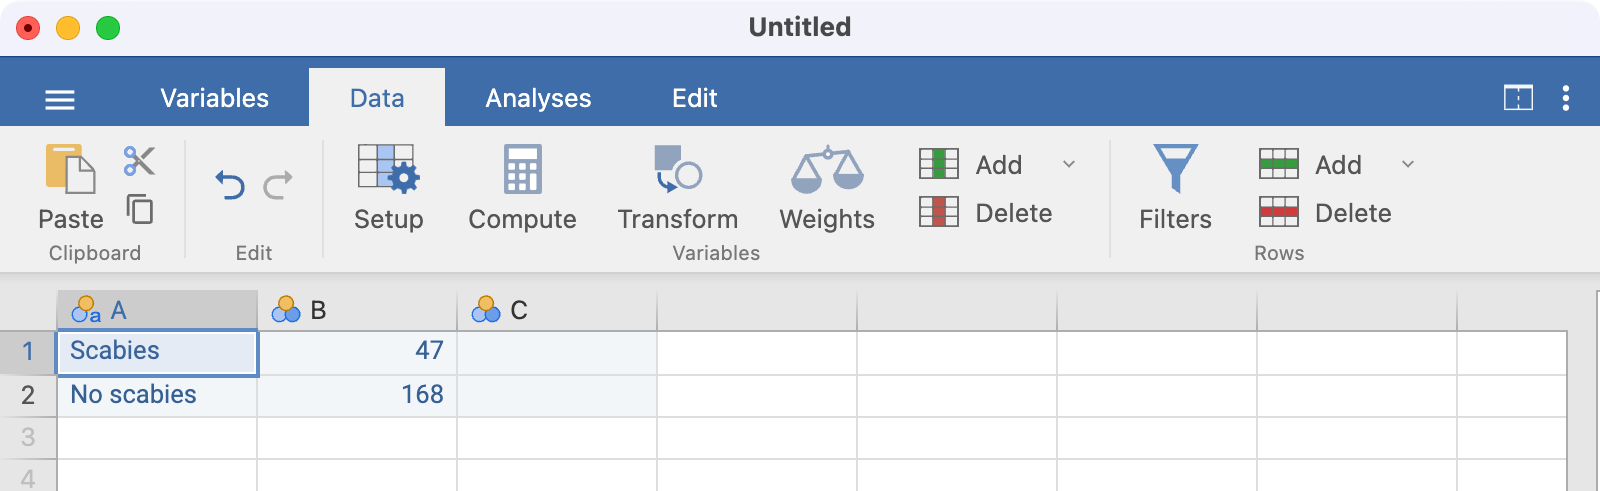
\includegraphics[keepaspectratio]{img/mod06/jamovi/mod06-prop-data.png}}

Note that there is no need to name the columns here; using \texttt{A}
and \texttt{B} is fine.

Before we analyse these data, we need to tell jamovi that column
\texttt{B} represents the count of each category. We do this by using
\textbf{Data \textgreater{} Weights} and defining \texttt{B} as the
weight variable. This essentially says that the first row represents 47
observations, and the second row represents 168 observations:

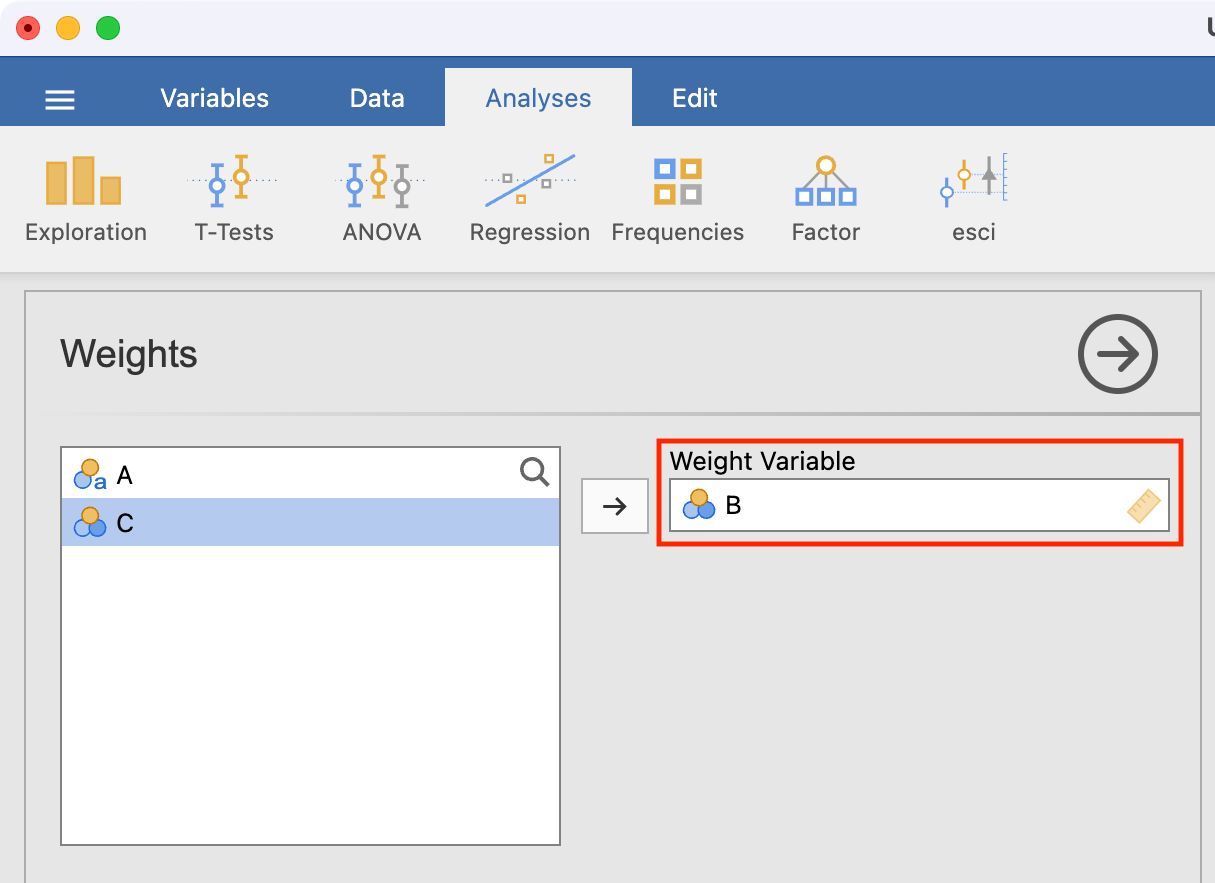
\includegraphics[width=0.8\linewidth,height=\textheight,keepaspectratio]{img/mod06/jamovi/mod06-prop-weight.png}

To estimate the proportion with scabies, we use \textbf{Frequencies
\textgreater{} One Sample Proportion Tests \textgreater{} 2 Outcomes
\textbar{} Binomial Test}, defining Column \texttt{A} as the analysis
variable and requesting confidence intervals\textbf{:}

\pandocbounded{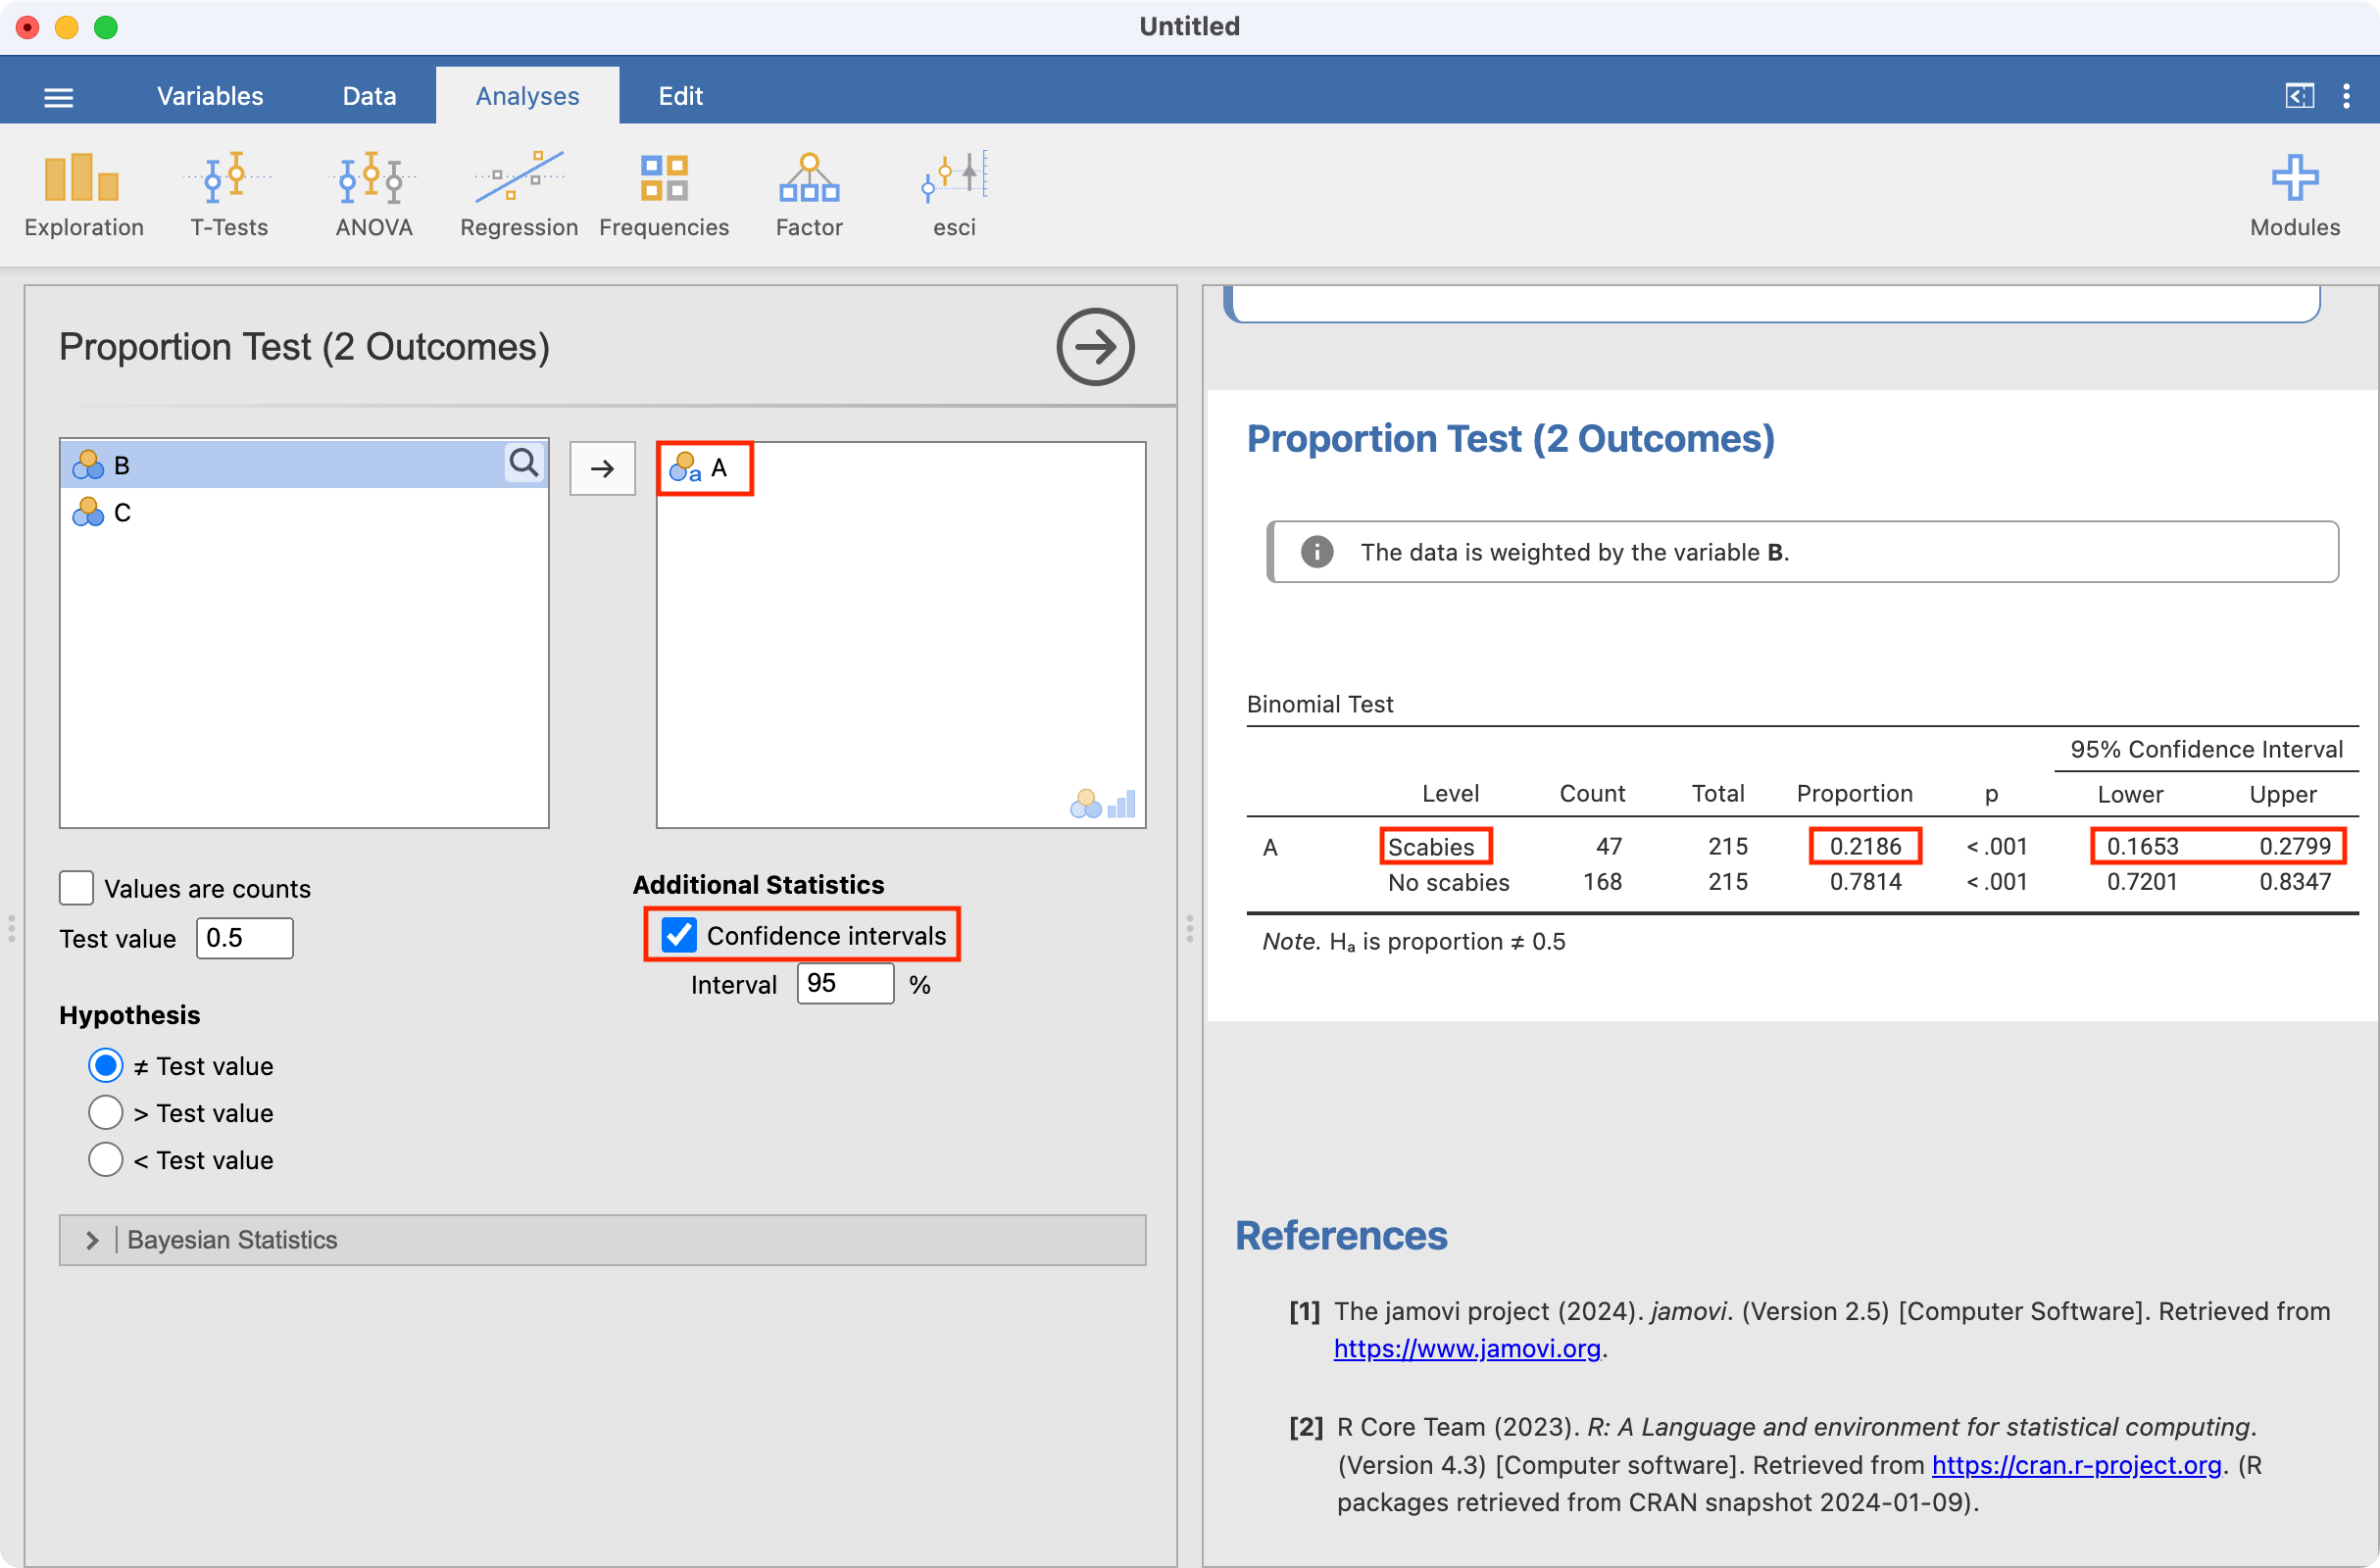
\includegraphics[keepaspectratio]{img/mod06/jamovi/mod06-prop-results.png}}

Note that the jamovi provides the proportion with scabies as well as the
proportion without scabies.

\subsection{Binomial test for testing one sample
proportion}\label{binomial-test-for-testing-one-sample-proportion-1}

A binomial test can be performed using a similar approach. Here we
consider Worked example 6.3, testing whether a sample is consistent with
a true smoking proportion of 20\%. \texttt{mod06\_smoking\_status.rds}
contains individual level data, so we do not need to use weighting.

After opening the data, click \textbf{Analyses \textgreater{}
Frequencies \textgreater{} One Sample Proportion Tests \textgreater{} 2
Outcomes \textbar{} Binomial Test}. Set the \textbf{Test value} as 0.2,
and tick the \textbf{Confidence intervals} box:

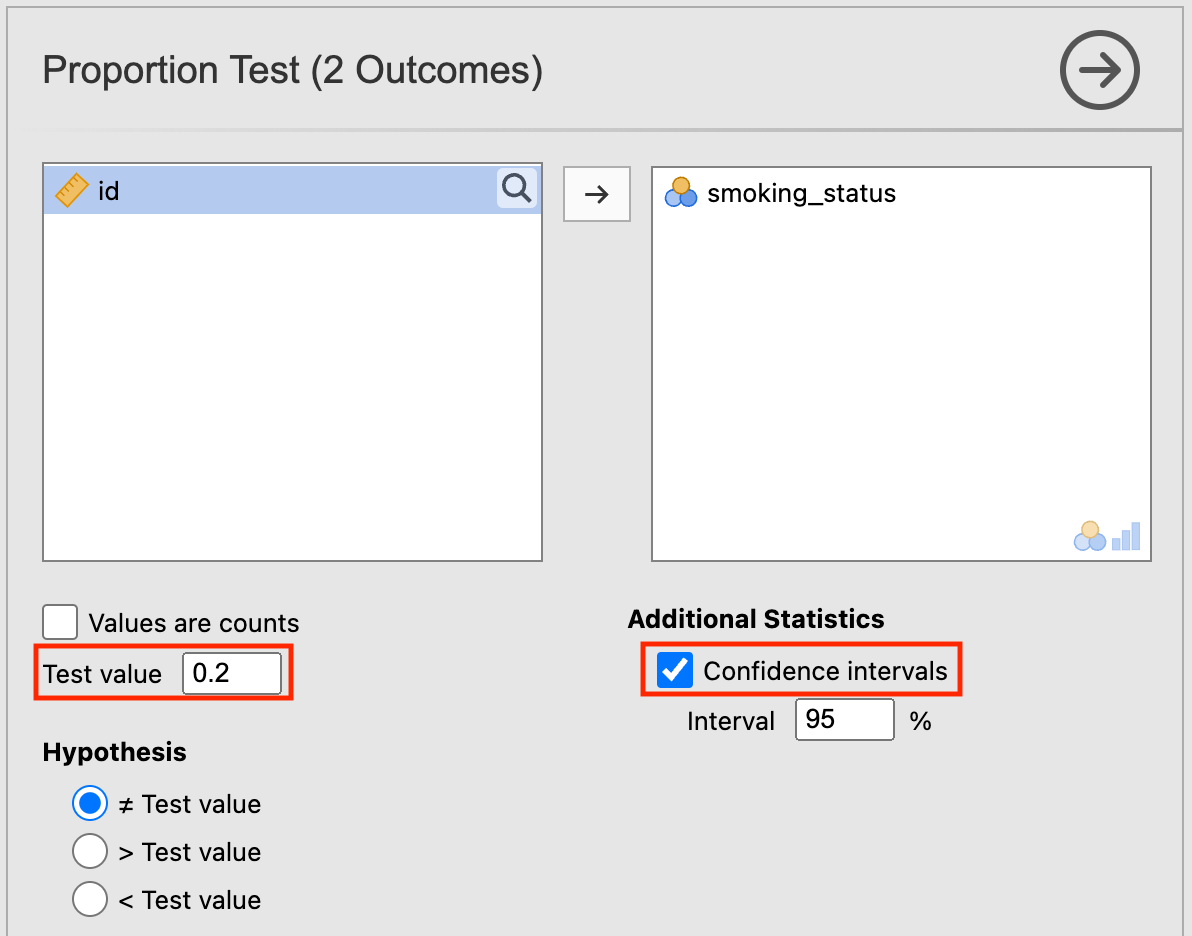
\includegraphics[width=0.75\linewidth,height=\textheight,keepaspectratio]{img/mod06/jamovi/mod06-prop-test.png}

The P-value for testing whether the true proportion of smokers is 20\%
is provided as P=0.43:

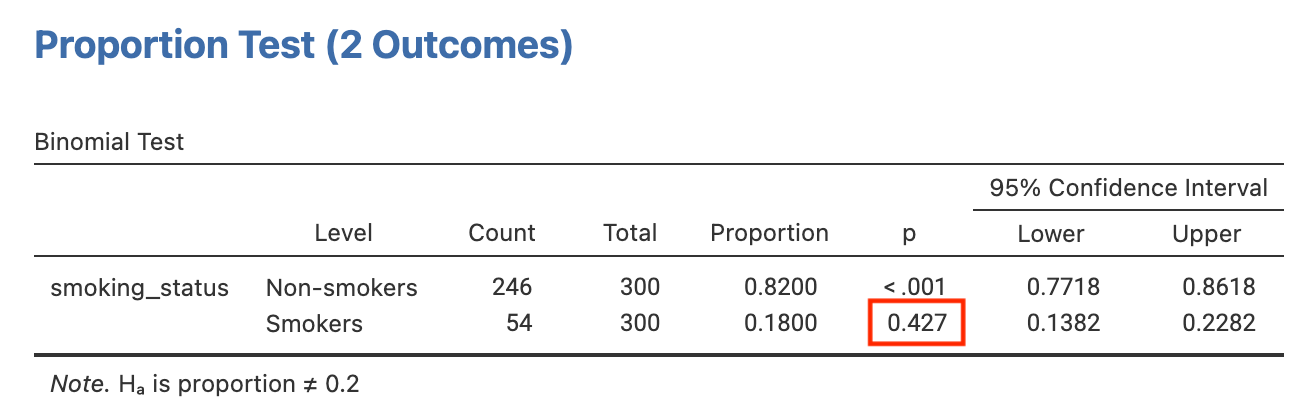
\includegraphics[width=0.5\linewidth,height=\textheight,keepaspectratio]{img/mod06/jamovi/mod06-prop-test-result.png}

\section{Computing a relative risk and its 95\% confidence
interval}\label{computing-a-relative-risk-and-its-95-confidence-interval}

To calculate relative risks, odds ratios and risk differences correctly,
\textbf{we must define the positive exposure and positive outcome to be
the first level of a factor}. When defining an exposure for example, we
should define the active treatment or the positive exposure as the first
category. When defining an outcome, we should define the category of
interest (e.g.~disease, or side effect) as the first category.

We will use Worked Example 6.4 to demonstrate calculating a relative
risk and its 95\% CI, by opening \texttt{mod06\_nausea.rds}.

Before analysing these data, we should check that the exposure
(\texttt{group}) and outcome (\texttt{side\_effect}) variables have been
set up correctly, with the correct level chosen to be of interest. In
this example, we will define \texttt{Active} as the first level in the
\texttt{group} factor, and \texttt{Nausea} to be the first level of the
\texttt{side\_effect} factor. Let's consider the exposure variable
first. Click \textbf{Data \textgreater{} Setup} - this will open the
following window:

\pandocbounded{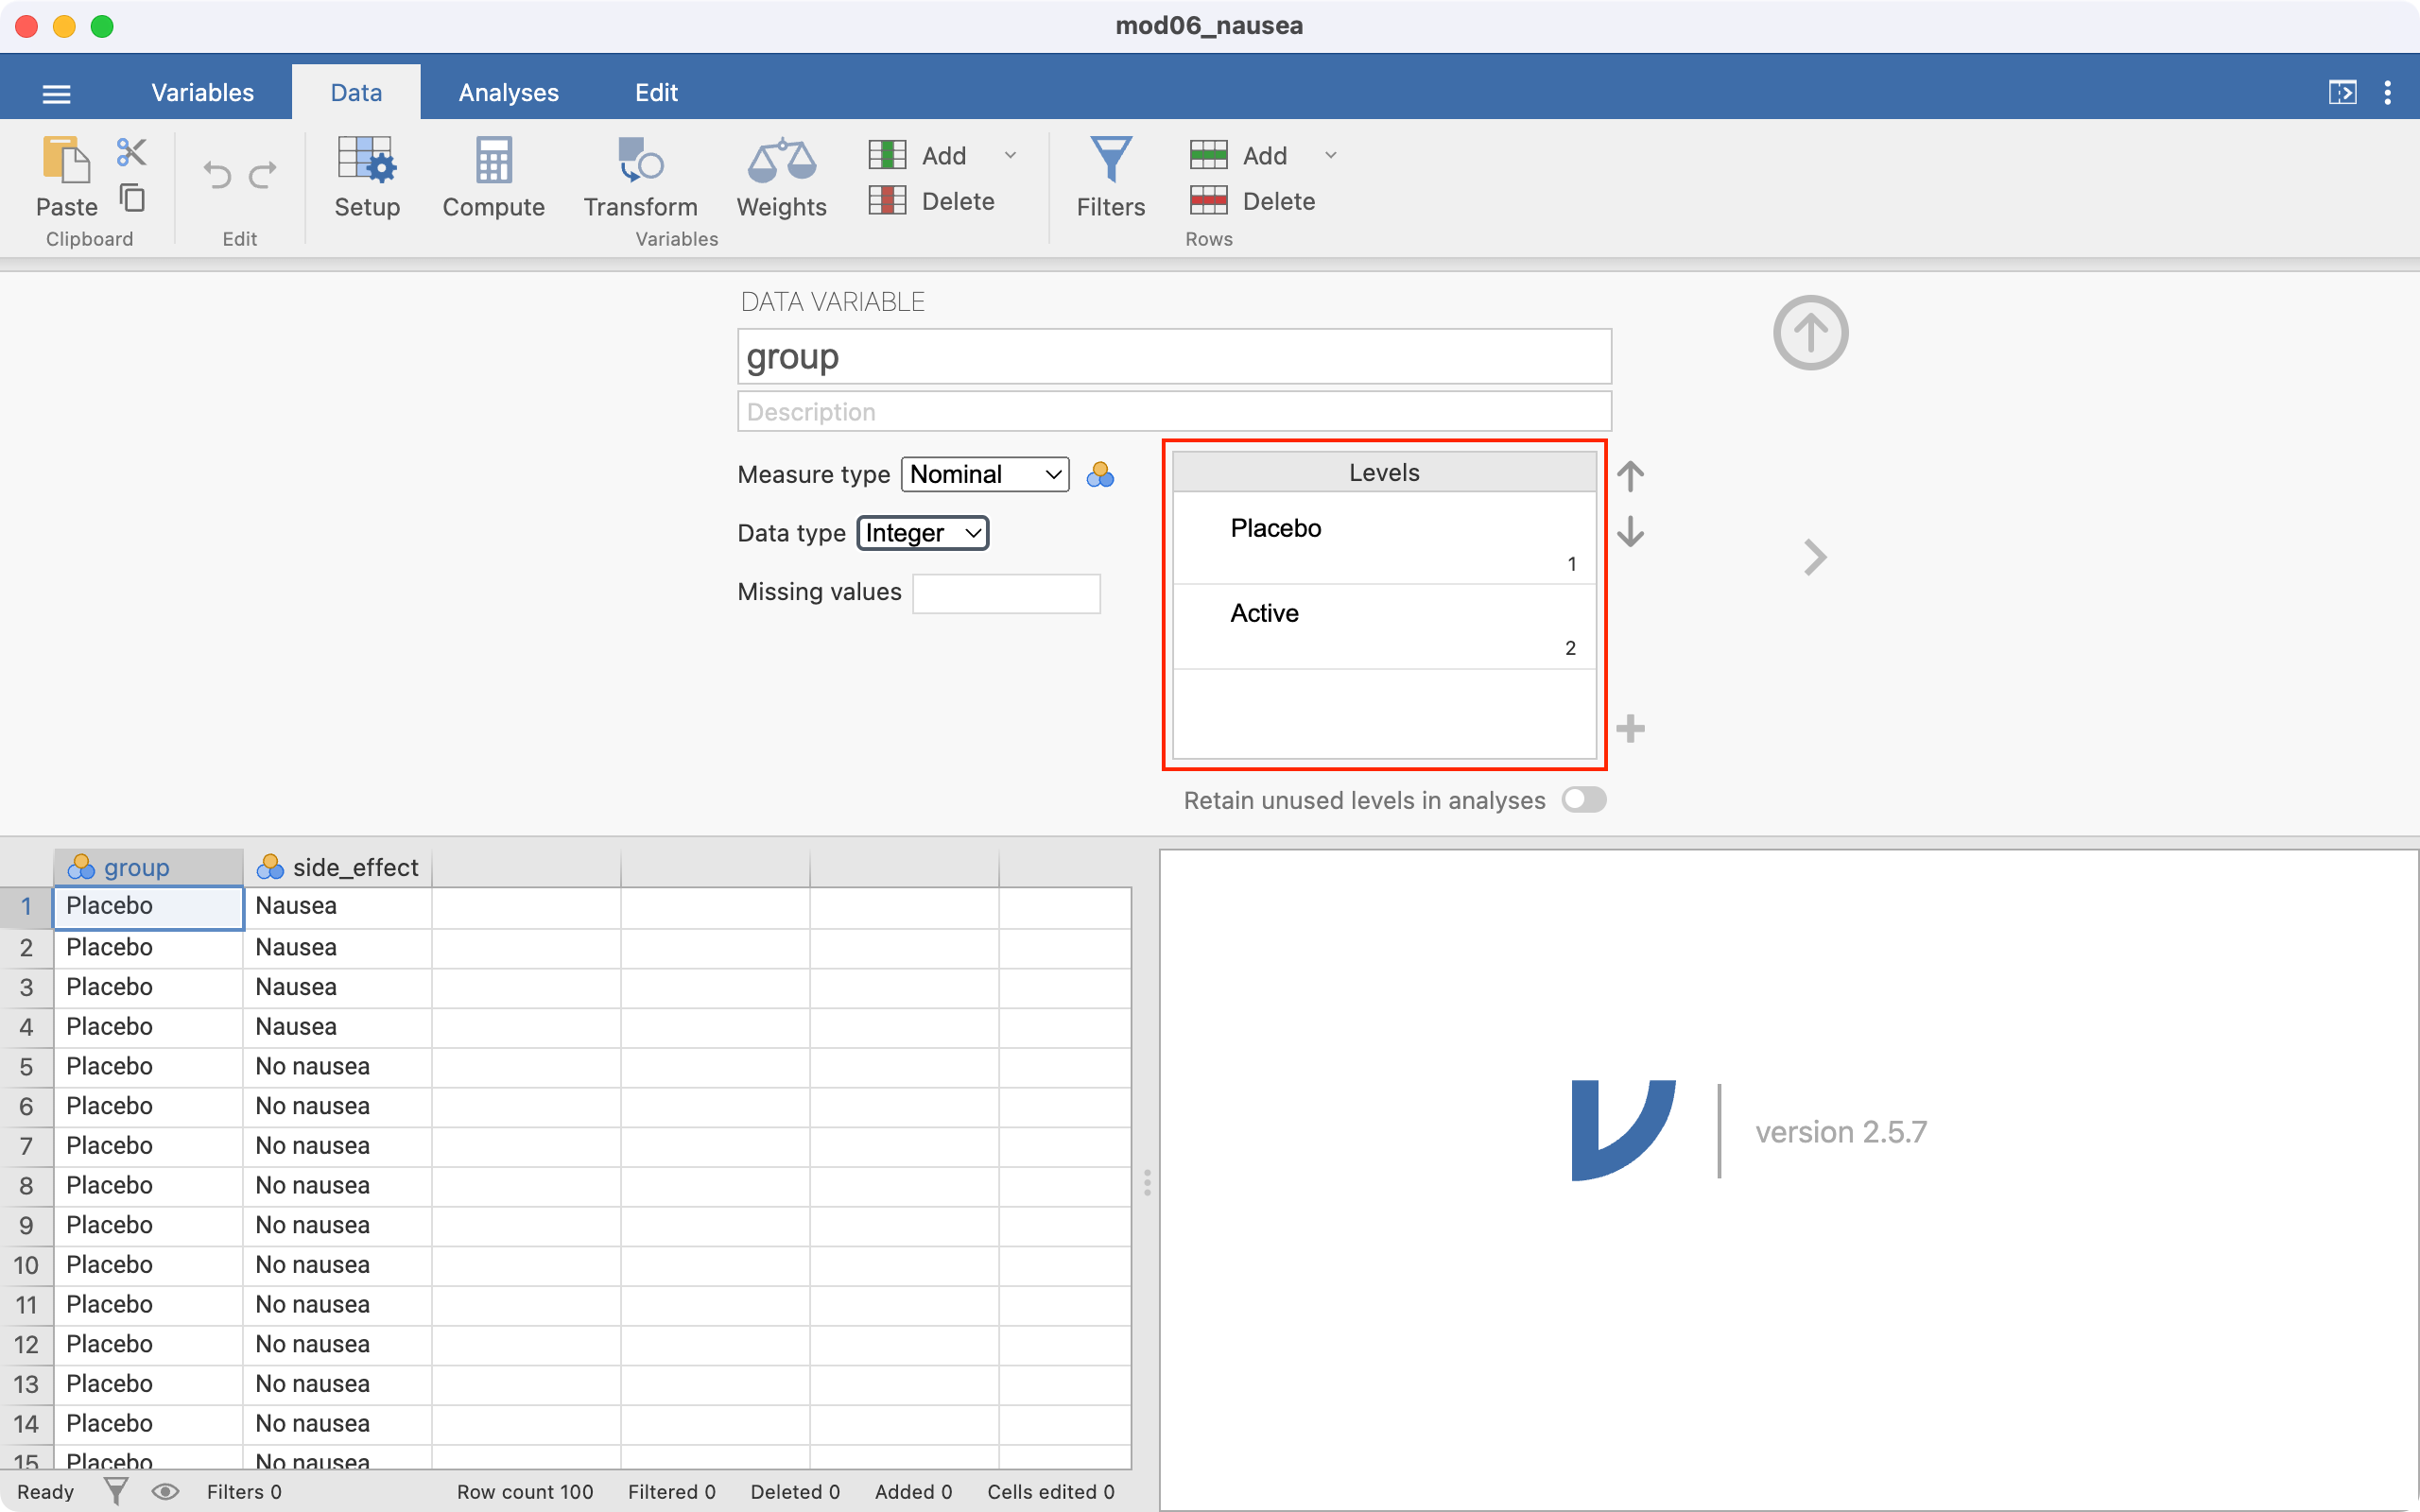
\includegraphics[keepaspectratio]{img/mod06/jamovi/refactor-1.png}}

Notice the \textbf{Levels} section, highlighted in red. This means that
that the \texttt{group} variable has been entered in jamovi with
\emph{Placebo} as the first category, and \emph{Active} as the second.
This ordering means that jamovi will incorrectly consider \emph{Placebo}
as ``Exposed'', and \emph{Active} as ``Unexposed''. We need to change
the ordering, so that \emph{Active} is the first level, and
\emph{Placebo} is second.

To re-order the levels:

\begin{enumerate}
\def\labelenumi{\arabic{enumi}.}
\item
  click the \emph{Placebo} cell in the \textbf{Levels} box, then
\item
  click the down arrow to move \emph{Placebo} to be the second level:
\end{enumerate}

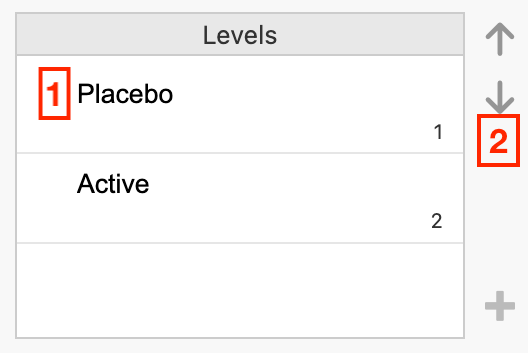
\includegraphics[width=0.5\linewidth,height=\textheight,keepaspectratio]{img/mod06/jamovi/refactor-2.png}

The \textbf{Levels} section should appear as below:

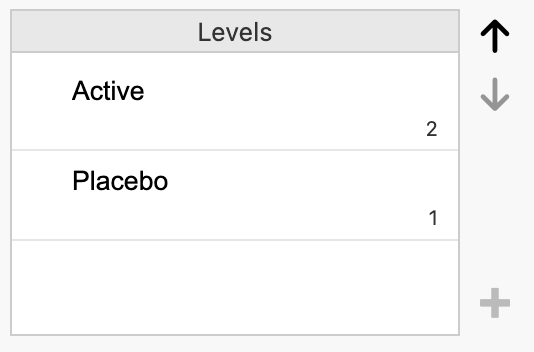
\includegraphics[width=0.5\linewidth,height=\textheight,keepaspectratio]{img/mod06/jamovi/refactor-3.png}

Click the \texttt{side\_effect} column to investigate the ordering of
the outcome variable. Repeat the process to set \emph{Nausea} as the
first level, and \emph{No nausea} as the second variable.

To construct the 2-by-2 table and calculate a relative risk, we use
\textbf{Analyses \textgreater{} Frequencies \textgreater{} Independent
samples}. Define \textbf{Rows} as the exposure variable
(\texttt{group}), and \textbf{Columns} as the outcome
(\texttt{side\_effect}). We can request the row-percents by ticking
\textbf{Row} in the \textbf{Cells} section, and request the relative
risk and confidence interval by ticking \textbf{Relative risk} in the
\textbf{Statistics} section:

\pandocbounded{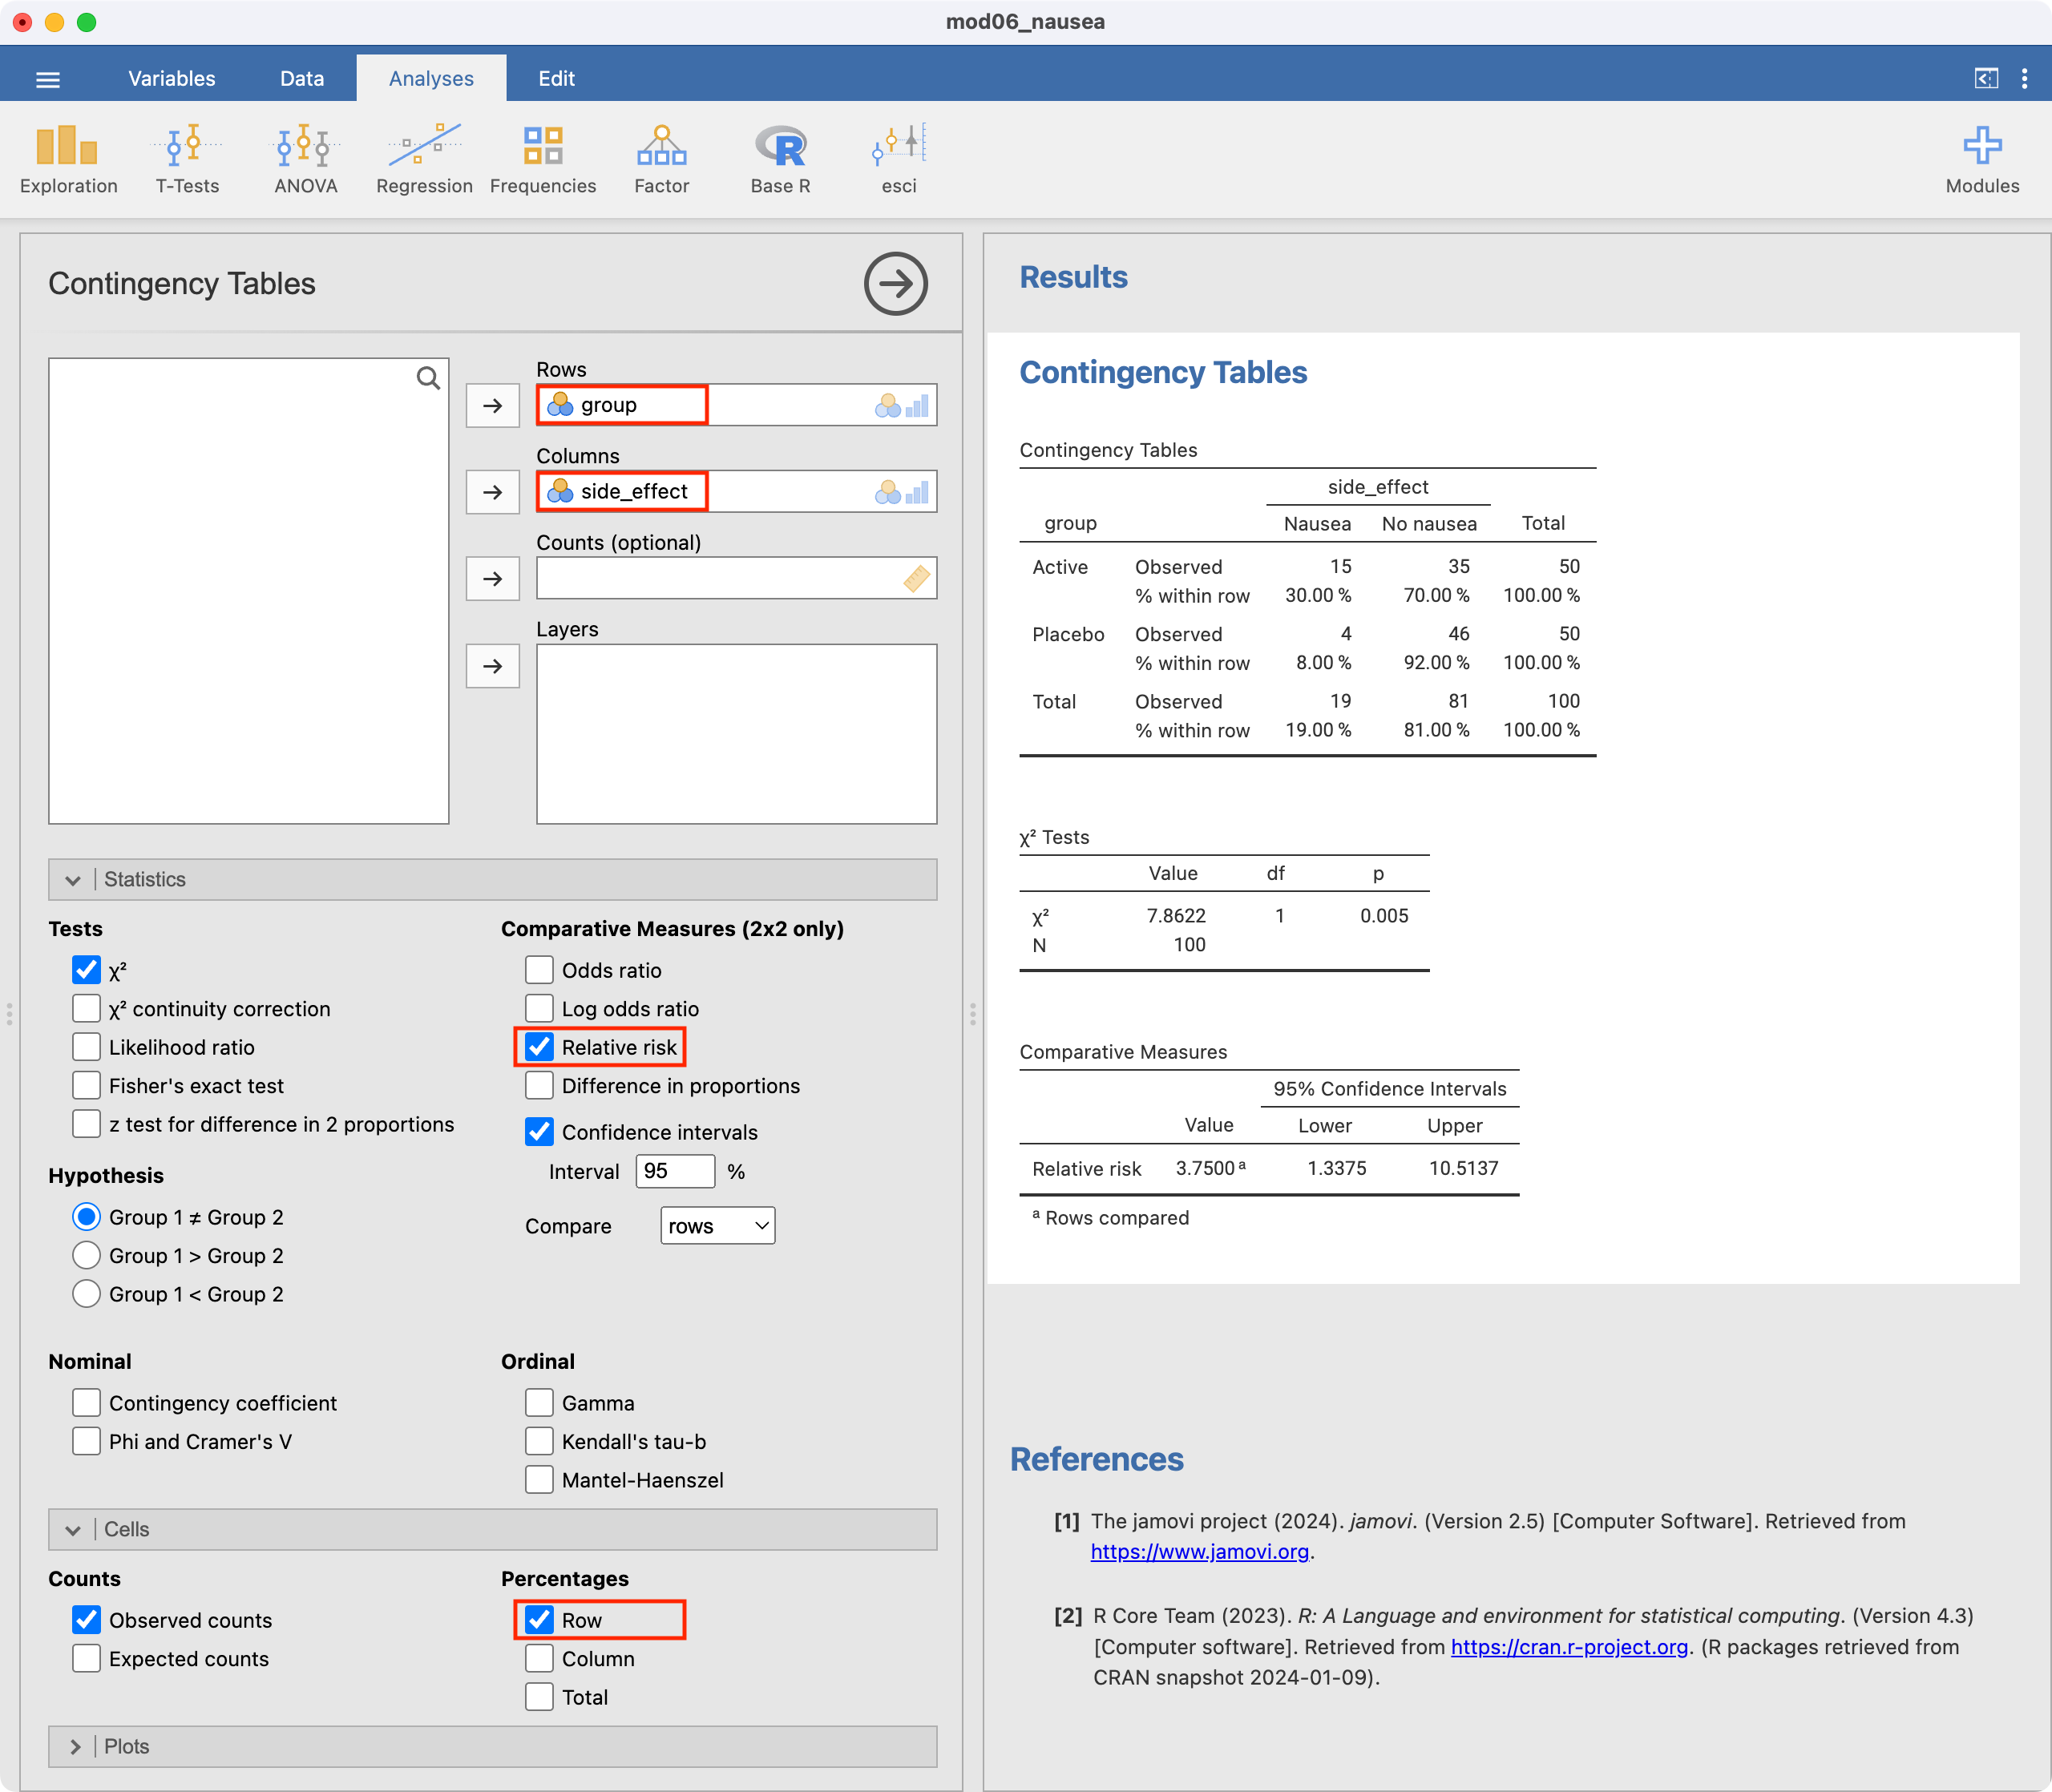
\includegraphics[keepaspectratio]{img/mod06/jamovi/rr.png}}

\section{Computing other measures of
effect}\label{computing-other-measures-of-effect}

An \textbf{Odds ratio} or \textbf{Difference in proportions} can be
requested in the \textbf{Statistics} section.

\section{Working with summarised
data}\label{working-with-summarised-data}

If you only have the cross-tabulated data (i.e.~the summarised or
aggregated data), you will need to enter your data into a new
spreadsheet. For example, to recreate the above analyses, we could
re-write the 2-by-2 table as follows:

{\def\LTcaptype{none} % do not increment counter
\begin{longtable}[]{@{}ccc@{}}
\toprule\noalign{}
Group & Side effect & Count \\
\midrule\noalign{}
\endhead
\bottomrule\noalign{}
\endlastfoot
Active & Nausea & 15 \\
Active & No nausea & 35 \\
Placebo & Nausea & 4 \\
Placebo & No nausea & 46 \\
\end{longtable}
}

We can enter these data in a new spreadsheet, entering the exposure and
outcome using the values of 0 or 1. By convention, we use 1 to represent
the exposed category, and 0 to represent the unexposed category.
Similarly, we use 1 to represent the outcome category of interest, and 0
to represent the outcome category not of interest. Our entered data
would look as follows:

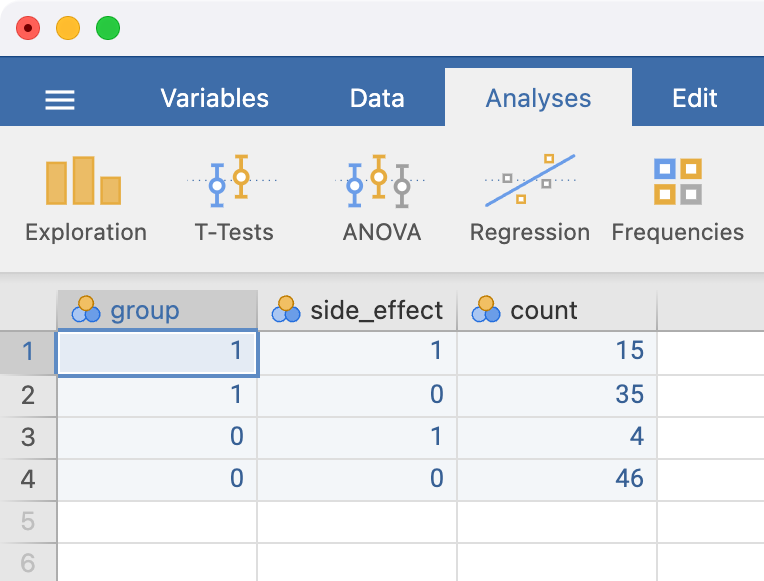
\includegraphics[width=0.5\linewidth,height=\textheight,keepaspectratio]{img/mod06/jamovi/aggregate-1.png}

The variable names can be changed in the variables tab in the usual way.
It is good practice to label the \textbf{levels} of the exposure and
outcome variables - this can be done in \textbf{Data \textgreater{}
Setup}. Click the variable to be defined, and type the labels of each
level in the \textbf{Levels} section.

Here, the variable \textbf{group} is defined as:

\begin{itemize}
\tightlist
\item
  1 represents Active
\item
  0 represents Placebo
\end{itemize}

The \textbf{Setup} screen is completed as follows:

\pandocbounded{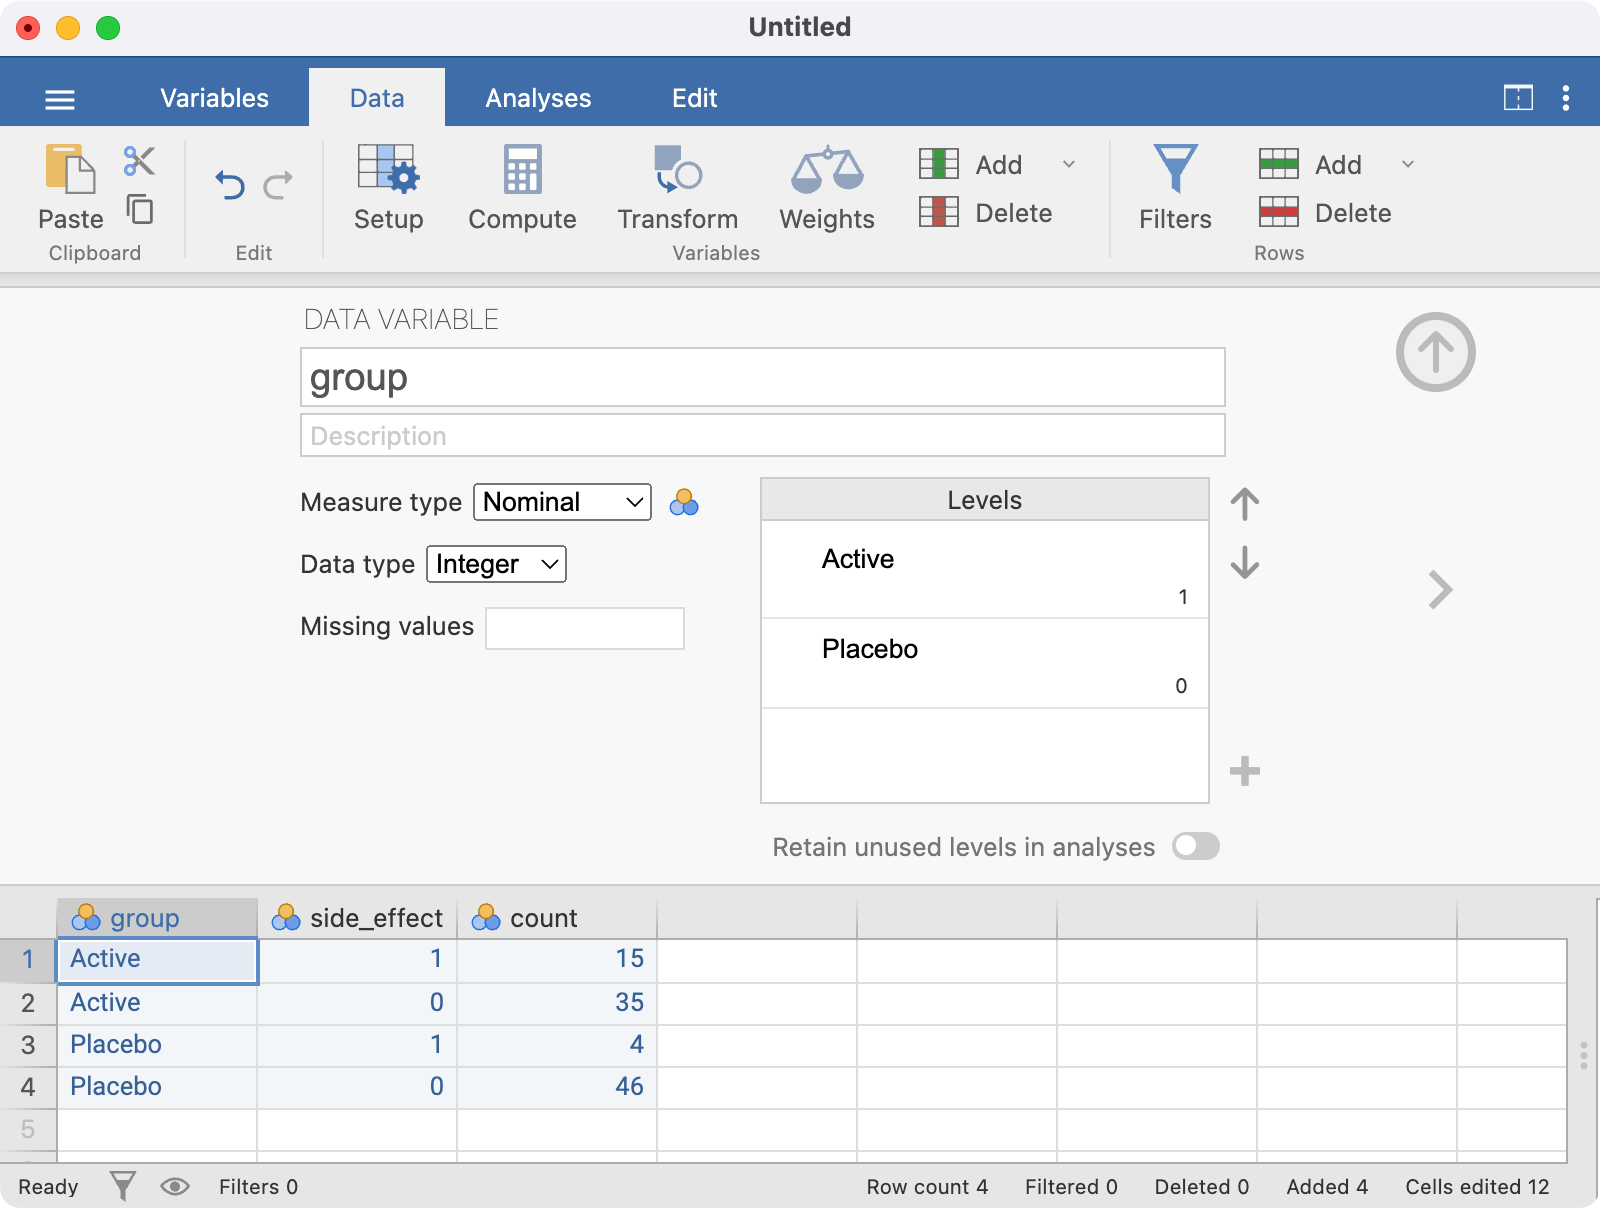
\includegraphics[keepaspectratio]{img/mod06/jamovi/aggregate-2.png}}

The \texttt{side\_effect} variable should be set up using a similar
approach, with the final spreadsheet looking like:

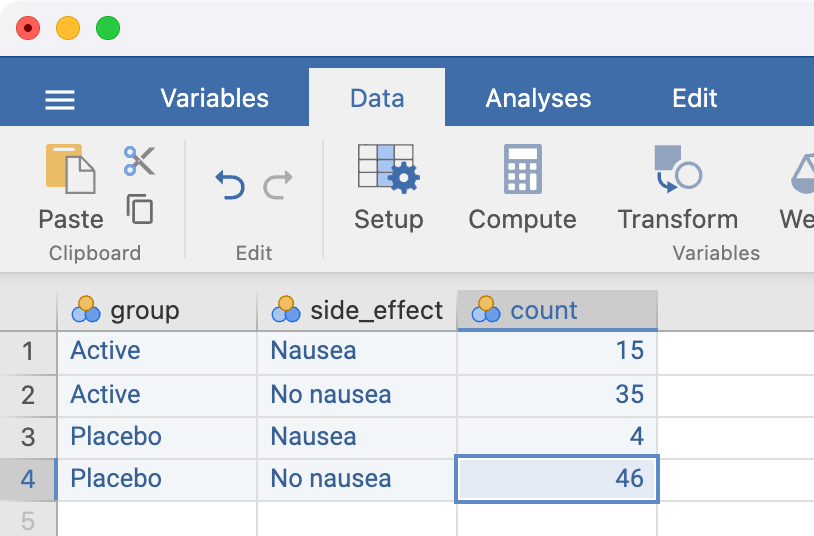
\includegraphics[width=0.5\linewidth,height=\textheight,keepaspectratio]{img/mod06/jamovi/aggregate-3.png}

The analysis is conducted in the same way as for individual data, but we
must now specify the \textbf{Counts} field:

\pandocbounded{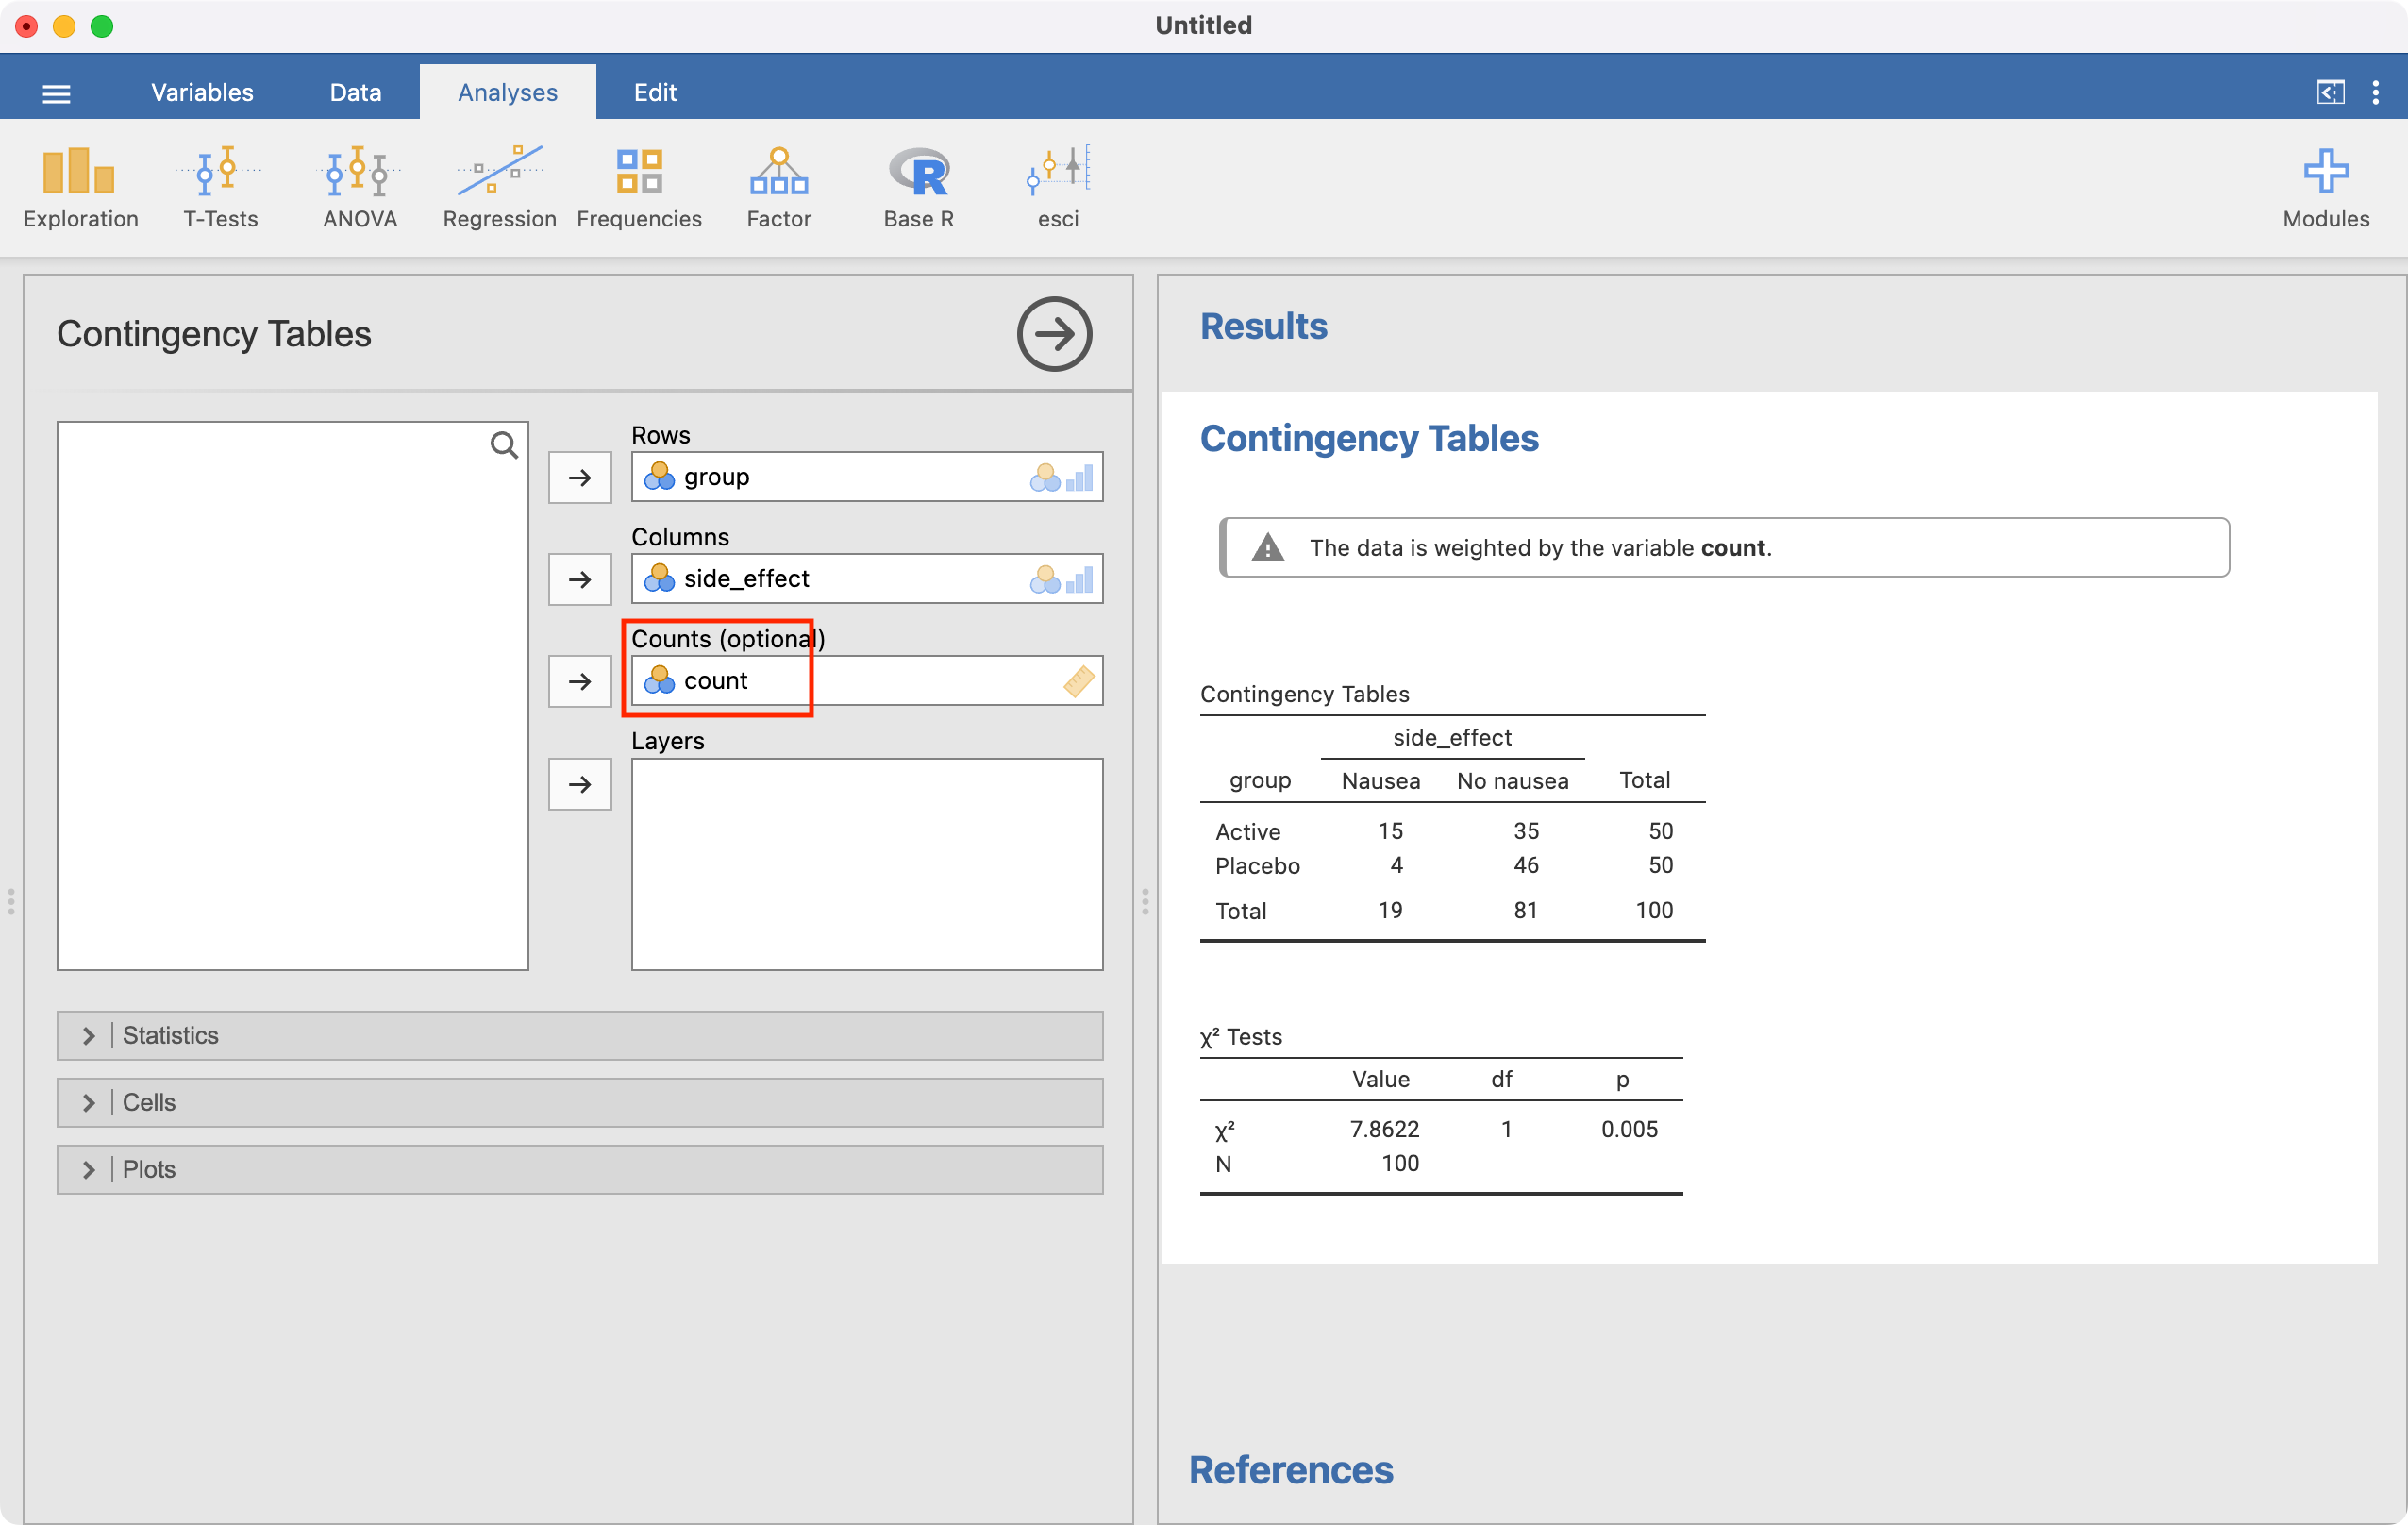
\includegraphics[keepaspectratio]{img/mod06/jamovi/aggregate-4.png}}

\newpage{}

\bookmarksetup{startatroot}

\chapter*{R notes}\label{r-notes-4}
\addcontentsline{toc}{chapter}{R notes}

\markboth{R notes}{R notes}

\section{95\% confidence intervals for
proportions}\label{confidence-intervals-for-proportions-1}

We can use the \texttt{BinomCI(x=,\ n=,\ method=)} function within the
\texttt{DescTools} package to compute 95\% confidence intervals for
proportions. Here we specify \texttt{x}: the number of successes,
\texttt{n}: the sample size, and optionally, the \texttt{method} (which
defaults to Wilson's method).

\begin{Shaded}
\begin{Highlighting}[]
\FunctionTok{library}\NormalTok{(DescTools)}

\FunctionTok{BinomCI}\NormalTok{(}\AttributeTok{x=}\DecValTok{47}\NormalTok{, }\AttributeTok{n=}\DecValTok{215}\NormalTok{, }\AttributeTok{method=}\StringTok{\textquotesingle{}wald\textquotesingle{}}\NormalTok{)}
\end{Highlighting}
\end{Shaded}

\begin{verbatim}
           est    lwr.ci    upr.ci
[1,] 0.2186047 0.1633595 0.2738498
\end{verbatim}

\begin{Shaded}
\begin{Highlighting}[]
\FunctionTok{BinomCI}\NormalTok{(}\AttributeTok{x=}\DecValTok{47}\NormalTok{, }\AttributeTok{n=}\DecValTok{215}\NormalTok{, }\AttributeTok{method=}\StringTok{\textquotesingle{}wilson\textquotesingle{}}\NormalTok{)}
\end{Highlighting}
\end{Shaded}

\begin{verbatim}
           est    lwr.ci    upr.ci
[1,] 0.2186047 0.1685637 0.2785246
\end{verbatim}

\section{Significance test for single
proportion}\label{significance-test-for-single-proportion}

We can use the \texttt{binom.test} function to perform a significance
test for a single proportion: \texttt{binom.test(x=,\ n=,\ p=)}. Here we
specify \texttt{x}: the number of successes, \texttt{n}: the sample
size, and \texttt{p}: the hypothesised proportion (which defaults to 0.5
if nothing is entered).

\begin{Shaded}
\begin{Highlighting}[]
\FunctionTok{binom.test}\NormalTok{(}\AttributeTok{x=}\DecValTok{54}\NormalTok{, }\AttributeTok{n=}\DecValTok{300}\NormalTok{, }\AttributeTok{p=}\FloatTok{0.2}\NormalTok{)}
\end{Highlighting}
\end{Shaded}

\begin{verbatim}

    Exact binomial test

data:  54 and 300
number of successes = 54, number of trials = 300, p-value = 0.4273
alternative hypothesis: true probability of success is not equal to 0.2
95 percent confidence interval:
 0.1382104 0.2282394
sample estimates:
probability of success 
                  0.18 
\end{verbatim}

Note that the \texttt{binom.test} function also produces a 95\%
confidence interval around the estimated proportion. This confidence
interval is based on the inferior Wald method: \emph{the confidence
interval derived from the Wilson method is preferred}.

We can also conduct a z-test for a single proportion:

\begin{Shaded}
\begin{Highlighting}[]
\FunctionTok{prop.test}\NormalTok{(}\AttributeTok{x=}\DecValTok{54}\NormalTok{, }\AttributeTok{n=}\DecValTok{300}\NormalTok{, }\AttributeTok{p=}\FloatTok{0.2}\NormalTok{, }\AttributeTok{correct=}\ConstantTok{FALSE}\NormalTok{)}
\end{Highlighting}
\end{Shaded}

\begin{verbatim}

    1-sample proportions test without continuity correction

data:  54 out of 300, null probability 0.2
X-squared = 0.75, df = 1, p-value = 0.3865
alternative hypothesis: true p is not equal to 0.2
95 percent confidence interval:
 0.1406583 0.2274332
sample estimates:
   p 
0.18 
\end{verbatim}

\section{Computing a relative risk and its 95\% confidence
interval}\label{computing-a-relative-risk-and-its-95-confidence-interval-1}

We will use Worked Example 6.4 to demonstrate calculating a relative
risk and its 95\% CI:

\begin{Shaded}
\begin{Highlighting}[]
\FunctionTok{library}\NormalTok{(jmv)}
\FunctionTok{library}\NormalTok{(dplyr)}

\NormalTok{drug }\OtherTok{\textless{}{-}} \FunctionTok{readRDS}\NormalTok{(}\StringTok{"data/examples/mod06\_nausea.rds"}\NormalTok{)}

\FunctionTok{summary}\NormalTok{(drug)}
\end{Highlighting}
\end{Shaded}

\begin{verbatim}
     group       side_effect
 Placebo:50   No nausea:81  
 Active :50   Nausea   :19  
\end{verbatim}

By using the \texttt{head()} function to view the first six lines of
data, we see that both \texttt{group} and \texttt{side\_effect} have
been entered as factors. Notice the order in which the factor levels are
presented: \texttt{group} has the \texttt{Placebo} level defined as the
first level, and the \texttt{Active} level defined as the second;
\texttt{side\_effect} has \texttt{No\ nausea} defined as the first
level, and the \texttt{Nausea} level defined as the second.

We will use \texttt{jmv} to calculate relative risks, odds ratios and
risk differences. To calculate these estimates correctly, \textbf{we
must define the positive exposure and positive outcome to be the first
level of a factor}. When defining an exposure for example, we should
define the active treatment or the positive exposure as the first
category. When defining an outcome, we should define the category of
interest (e.g.~disease, or side effect) as the first category.

In this example, we will define \texttt{Active} as the first level in
the \texttt{group} factor, and \texttt{Nausea} to be the first level of
the \texttt{side\_effect} factor.

We can do this using the \texttt{relevel()} function, which re-orders
the levels of a factor so that the level specified is defined as the
first level, and the others are moved down:

\begin{Shaded}
\begin{Highlighting}[]
\CommentTok{\# Define "Active" as the first level of group and "Nausea" as the first level of side\_effect:}
\NormalTok{drug }\OtherTok{\textless{}{-}} \FunctionTok{mutate}\NormalTok{(drug, }\AttributeTok{group =} \FunctionTok{relevel}\NormalTok{(group, }\AttributeTok{ref=}\StringTok{"Active"}\NormalTok{),}
                     \AttributeTok{side\_effect =} \FunctionTok{relevel}\NormalTok{(side\_effect, }\AttributeTok{ref=}\StringTok{"Nausea"}\NormalTok{))}
\end{Highlighting}
\end{Shaded}

Upon re-leveling the factors, we can check that the levels of interest
have been defined as the first levels:

\begin{Shaded}
\begin{Highlighting}[]
\FunctionTok{summary}\NormalTok{(drug)}
\end{Highlighting}
\end{Shaded}

\begin{verbatim}
     group       side_effect
 Active :50   Nausea   :19  
 Placebo:50   No nausea:81  
\end{verbatim}

To construct the 2-by-2 table and calculate a relative risk, we use the
\texttt{contTables()} function in \texttt{jmv}. We request the
row-percents using \texttt{pcRow\ =\ TRUE} and the relative risk and
confidence interval using \texttt{relRisk\ =\ TRUE}:

\begin{Shaded}
\begin{Highlighting}[]
\FunctionTok{contTables}\NormalTok{(}\AttributeTok{data=}\NormalTok{drug, }
           \AttributeTok{rows=}\NormalTok{group, }\AttributeTok{cols=}\NormalTok{side\_effect, }
           \AttributeTok{pcRow=}\ConstantTok{TRUE}\NormalTok{, }\AttributeTok{relRisk =} \ConstantTok{TRUE}\NormalTok{)}
\end{Highlighting}
\end{Shaded}

\begin{verbatim}

 CONTINGENCY TABLES

 Contingency Tables                                                 
 ────────────────────────────────────────────────────────────────── 
   group                      Nausea       No nausea    Total       
 ────────────────────────────────────────────────────────────────── 
   Active     Observed               15           35           50   
              % within row     30.00000     70.00000    100.00000   
                                                                    
   Placebo    Observed                4           46           50   
              % within row      8.00000     92.00000    100.00000   
                                                                    
   Total      Observed               19           81          100   
              % within row     19.00000     81.00000    100.00000   
 ────────────────────────────────────────────────────────────────── 


 χ² Tests                              
 ───────────────────────────────────── 
         Value       df    p           
 ───────────────────────────────────── 
   χ²    7.862248     1    0.0050478   
   N          100                      
 ───────────────────────────────────── 


 Comparative Measures                                    
 ─────────────────────────────────────────────────────── 
                    Value         Lower       Upper      
 ─────────────────────────────────────────────────────── 
   Relative risk    3.750000 ᵃ    1.337540    10.51370   
 ─────────────────────────────────────────────────────── 
   ᵃ Rows compared
\end{verbatim}

If you only have the cross-tabulated data (i.e.~aggregated), you will
need to enter your data into a new data frame. For example, to recreate
the above analyses, we can re-write the 2-by-2 table as follows:

{\def\LTcaptype{none} % do not increment counter
\begin{longtable}[]{@{}ccc@{}}
\toprule\noalign{}
Group & side\_effect & Number \\
\midrule\noalign{}
\endhead
\bottomrule\noalign{}
\endlastfoot
Active & Nausea & 15 \\
Active & No nausea & 35 \\
Placebo & Nausea & 4 \\
Placebo & No nausea & 46 \\
\end{longtable}
}

We can enter these data in a dataframe, comprising three vectors, as
follows:

\begin{Shaded}
\begin{Highlighting}[]
\NormalTok{drug\_aggregated }\OtherTok{\textless{}{-}} \FunctionTok{data.frame}\NormalTok{(}
  \AttributeTok{group =} \FunctionTok{c}\NormalTok{(}\StringTok{"Active"}\NormalTok{, }\StringTok{"Active"}\NormalTok{, }\StringTok{"Placebo"}\NormalTok{, }\StringTok{"Placebo"}\NormalTok{),}
  \AttributeTok{side\_effect =} \FunctionTok{c}\NormalTok{(}\StringTok{"Nausea"}\NormalTok{, }\StringTok{"No nausea"}\NormalTok{, }\StringTok{"Nausea"}\NormalTok{, }\StringTok{"No nausea"}\NormalTok{),}
  \AttributeTok{n =} \FunctionTok{c}\NormalTok{(}\DecValTok{15}\NormalTok{, }\DecValTok{35}\NormalTok{, }\DecValTok{4}\NormalTok{, }\DecValTok{46}\NormalTok{))}
\end{Highlighting}
\end{Shaded}

We need to define group and side\_effect as factors. Here we must define
the \texttt{levels} \textbf{in the order we want the categories to
appear in the table}. Note that as group and side\_effect are entered as
text variables, we can omit \texttt{labels} command when defining the
factors, and the factor will be labelled using the text entry:

\begin{Shaded}
\begin{Highlighting}[]
\NormalTok{drug\_aggregated }\OtherTok{=} \FunctionTok{mutate}\NormalTok{(drug\_aggregated,}
                         \AttributeTok{group =} \FunctionTok{factor}\NormalTok{(group, }\AttributeTok{levels=}\FunctionTok{c}\NormalTok{(}\StringTok{"Active"}\NormalTok{, }\StringTok{"Placebo"}\NormalTok{)),}
                         \AttributeTok{side\_effect =} \FunctionTok{factor}\NormalTok{(side\_effect, }\AttributeTok{levels=}\FunctionTok{c}\NormalTok{(}\StringTok{"Nausea"}\NormalTok{, }\StringTok{"No nausea"}\NormalTok{)))}
\end{Highlighting}
\end{Shaded}

We can calculate the relative risk using the summarised data in the same
was done previously. However, we need to include the number of
observations in each cell using the \texttt{counts} command:

\begin{Shaded}
\begin{Highlighting}[]
\FunctionTok{contTables}\NormalTok{(}\AttributeTok{data=}\NormalTok{drug\_aggregated,}
           \AttributeTok{rows=}\NormalTok{group, }\AttributeTok{cols=}\NormalTok{side\_effect, }\AttributeTok{count=}\NormalTok{n,}
           \AttributeTok{pcRow=}\ConstantTok{TRUE}\NormalTok{, }\AttributeTok{relRisk =} \ConstantTok{TRUE}\NormalTok{)}
\end{Highlighting}
\end{Shaded}

\begin{Shaded}
\begin{Highlighting}[]
\NormalTok{CONTINGENCY TABLES}

\NormalTok{ Contingency Tables                                                 }
\NormalTok{ ────────────────────────────────────────────────────────────────── }
\NormalTok{   group                      Nausea       No nausea    Total       }
\NormalTok{ ────────────────────────────────────────────────────────────────── }
\NormalTok{   Active     Observed        }\FloatTok{15.000000}     \FloatTok{35.00000}     \FloatTok{50.00000}   
\NormalTok{              \% within row     }\FloatTok{30.00000}     \FloatTok{70.00000}    \FloatTok{100.00000}   
                                                                    
\NormalTok{   Placebo    Observed         }\FloatTok{4.000000}     \FloatTok{46.00000}     \FloatTok{50.00000}   
\NormalTok{              \% within row      }\FloatTok{8.00000}     \FloatTok{92.00000}    \FloatTok{100.00000}   
                                                                    
\NormalTok{   Total      Observed        }\FloatTok{19.000000}     \FloatTok{81.00000}    \FloatTok{100.00000}   
\NormalTok{              \% within row     }\FloatTok{19.00000}     \FloatTok{81.00000}    \FloatTok{100.00000}   
\NormalTok{ ────────────────────────────────────────────────────────────────── }


\NormalTok{ χ² Tests                              }
\NormalTok{ ───────────────────────────────────── }
\NormalTok{         Value       df    p           }
\NormalTok{ ───────────────────────────────────── }
\NormalTok{   χ²    }\FloatTok{7.862248}     \DecValTok{1}    \FloatTok{0.0050478}   
\NormalTok{   N          }\DecValTok{100}                      
\NormalTok{ ───────────────────────────────────── }


\NormalTok{ Comparative Measures                                    }
\NormalTok{ ─────────────────────────────────────────────────────── }
\NormalTok{                    Value         Lower       Upper      }
\NormalTok{ ─────────────────────────────────────────────────────── }
\NormalTok{   Relative risk    }\FloatTok{3.750000}\NormalTok{ ᵃ    }\FloatTok{1.337540}    \FloatTok{10.51370}   
\NormalTok{ ─────────────────────────────────────────────────────── }
\NormalTok{   ᵃ Rows compared}
\end{Highlighting}
\end{Shaded}

\section{Computing a difference in proportions and its 95\% confidence
interval}\label{computing-a-difference-in-proportions-and-its-95-confidence-interval}

We can use the \texttt{contTables} function to obtain a difference in
proportions and its 95\% CI, by specifying \texttt{diffProp=TRUE}:

\begin{Shaded}
\begin{Highlighting}[]
\FunctionTok{contTables}\NormalTok{(}\AttributeTok{data=}\NormalTok{drug, }
           \AttributeTok{rows=}\NormalTok{group, }\AttributeTok{cols=}\NormalTok{side\_effect, }
           \AttributeTok{pcRow=}\ConstantTok{TRUE}\NormalTok{, }\AttributeTok{diffProp=}\ConstantTok{TRUE}\NormalTok{)}
\end{Highlighting}
\end{Shaded}

\begin{verbatim}

 CONTINGENCY TABLES

 Contingency Tables                                                 
 ────────────────────────────────────────────────────────────────── 
   group                      Nausea       No nausea    Total       
 ────────────────────────────────────────────────────────────────── 
   Active     Observed               15           35           50   
              % within row     30.00000     70.00000    100.00000   
                                                                    
   Placebo    Observed                4           46           50   
              % within row      8.00000     92.00000    100.00000   
                                                                    
   Total      Observed               19           81          100   
              % within row     19.00000     81.00000    100.00000   
 ────────────────────────────────────────────────────────────────── 


 χ² Tests                              
 ───────────────────────────────────── 
         Value       df    p           
 ───────────────────────────────────── 
   χ²    7.862248     1    0.0050478   
   N          100                      
 ───────────────────────────────────── 


 Comparative Measures                                                      
 ───────────────────────────────────────────────────────────────────────── 
                                  Value          Lower         Upper       
 ───────────────────────────────────────────────────────────────────────── 
   Difference in 2 proportions    0.2200000 ᵃ    0.07238986    0.3676101   
 ───────────────────────────────────────────────────────────────────────── 
   ᵃ Rows compared
\end{verbatim}

\section{Computing an odds ratio and its 95\% confidence
interval}\label{computing-an-odds-ratio-and-its-95-confidence-interval}

We can use the \texttt{contTables} function to obtain an odds ratio and
its 95\% CI, by specifying \texttt{odds=TRUE}. Here we will use the
summarised HPV data from Module 6.

\begin{Shaded}
\begin{Highlighting}[]
\NormalTok{hpv }\OtherTok{\textless{}{-}} \FunctionTok{data.frame}\NormalTok{(}
  \AttributeTok{hpv =} \FunctionTok{c}\NormalTok{(}\StringTok{"HPV +"}\NormalTok{, }\StringTok{"HPV +"}\NormalTok{, }\StringTok{"HPV {-}"}\NormalTok{, }\StringTok{"HPV {-}"}\NormalTok{),}
  \AttributeTok{cancer =} \FunctionTok{c}\NormalTok{(}\StringTok{"Case"}\NormalTok{, }\StringTok{"Control"}\NormalTok{, }\StringTok{"Case"}\NormalTok{, }\StringTok{"Control"}\NormalTok{),}
  \AttributeTok{n =} \FunctionTok{c}\NormalTok{(}\DecValTok{57}\NormalTok{, }\DecValTok{14}\NormalTok{, }\DecValTok{43}\NormalTok{, }\DecValTok{186}\NormalTok{)}
\NormalTok{)}

\NormalTok{hpv}\SpecialCharTok{$}\NormalTok{cancer }\OtherTok{\textless{}{-}} \FunctionTok{factor}\NormalTok{(hpv}\SpecialCharTok{$}\NormalTok{cancer, }\AttributeTok{levels=}\FunctionTok{c}\NormalTok{(}\StringTok{"Case"}\NormalTok{, }\StringTok{"Control"}\NormalTok{))}
\NormalTok{hpv}\SpecialCharTok{$}\NormalTok{hpv }\OtherTok{\textless{}{-}} \FunctionTok{factor}\NormalTok{(hpv}\SpecialCharTok{$}\NormalTok{hpv, }\AttributeTok{levels=}\FunctionTok{c}\NormalTok{(}\StringTok{"HPV +"}\NormalTok{, }\StringTok{"HPV {-}"}\NormalTok{))}

\FunctionTok{contTables}\NormalTok{(}\AttributeTok{data=}\NormalTok{hpv, }
           \AttributeTok{rows=}\NormalTok{hpv, }\AttributeTok{cols=}\NormalTok{cancer, }\AttributeTok{count=}\NormalTok{n,}
           \AttributeTok{odds =} \ConstantTok{TRUE}\NormalTok{)}
\end{Highlighting}
\end{Shaded}

\begin{Shaded}
\begin{Highlighting}[]
\NormalTok{ CONTINGENCY TABLES}

\NormalTok{ Contingency Tables                               }
\NormalTok{ ──────────────────────────────────────────────── }
\NormalTok{   hpv      Case         Control      Total       }
\NormalTok{ ──────────────────────────────────────────────── }
\NormalTok{   HPV }\SpecialCharTok{+}     \FloatTok{57.00000}     \FloatTok{14.00000}     \FloatTok{71.00000}   
\NormalTok{   HPV }\SpecialCharTok{{-}}     \FloatTok{43.00000}    \FloatTok{186.00000}    \FloatTok{229.00000}   
\NormalTok{   Total    }\FloatTok{100.00000}    \FloatTok{200.00000}    \FloatTok{300.00000}   
\NormalTok{ ──────────────────────────────────────────────── }


\NormalTok{ χ² Tests                               }
\NormalTok{ ────────────────────────────────────── }
\NormalTok{         Value       df    p            }
\NormalTok{ ────────────────────────────────────── }
\NormalTok{   χ²    }\FloatTok{92.25660}     \DecValTok{1}    \SpecialCharTok{\textless{}}\NormalTok{ .}\DecValTok{0000001}   
\NormalTok{   N          }\DecValTok{300}                       
\NormalTok{ ────────────────────────────────────── }


\NormalTok{ Comparative Measures                               }
\NormalTok{ ────────────────────────────────────────────────── }
\NormalTok{                 Value       Lower       Upper      }
\NormalTok{ ────────────────────────────────────────────────── }
\NormalTok{   Odds ratio    }\FloatTok{17.61130}    \FloatTok{8.992580}    \FloatTok{34.49041}   
\NormalTok{ ────────────────────────────────────────────────── }
\end{Highlighting}
\end{Shaded}

\newpage{}

\bookmarksetup{startatroot}

\chapter*{Activities}\label{activities-5}
\addcontentsline{toc}{chapter}{Activities}

\markboth{Activities}{Activities}

\subsection*{Activity 6.1}\label{activity-6.1}
\addcontentsline{toc}{subsection}{Activity 6.1}

In a clinical trial involving a dietary intervention, 150 adult
volunteers agreed to participate. The investigator wanted to know
whether this sample was representative of the general population. One
interesting finding was that 90 of the participants drank alcohol
regularly compared to 70\% of the general population.

\begin{enumerate}
\def\labelenumi{\alph{enumi})}
\tightlist
\item
  State the null hypothesis.
\item
  Calculate the proportion of regular drinkers (and its 95\% confidence
  interval) in the sample using software.
\item
  Conduct a hypothesis test to decide if the sample of volunteers is
  representative of the population.
\item
  Repeat (b) and (c) using the data saved in \texttt{Activity\_6.1.rds}.
\end{enumerate}

\subsection*{Activity 6.2}\label{activity-6.2}
\addcontentsline{toc}{subsection}{Activity 6.2}

A survey was conducted of a random sample of upper primary school
children to measure the prevalence of asthma using questionnaires
completed by the parents. A total of 514 children were enrolled. Use the
dataset \texttt{Activity\_6.2.rds} for this activity.

\begin{enumerate}
\def\labelenumi{\alph{enumi})}
\tightlist
\item
  What type of study was used to collect these data? Based on this,
  which measure of effect would you use to summarise the association
  between gender and asthma symptoms?
\item
  Calculate the relevant measure of effect (with its 95\% confidence
  interval).
\end{enumerate}

\subsection*{Activity 6.3}\label{activity-6.3}
\addcontentsline{toc}{subsection}{Activity 6.3}

A study is conducted to test the hypothesis that the observed frequency
of a certain health outcome is 30\%. If the results yield a CI around
the sample proportion that extends from 23.8 to 30.2, what can you say
about the evidence against the null hypothesis?

\subsection*{Activity 6.4}\label{activity-6.4}
\addcontentsline{toc}{subsection}{Activity 6.4}

In an experiment to test the effect of Vitamin C on IQ scores, the
following confidence intervals were estimated around the percentage with
improved scores for five different populations
(Table~\ref{tbl-act-6-5}):

\begin{table}[h]

\caption{\label{tbl-act-6-5}Study results from five difference
populations}

\centering{

\centering
\begin{tblr}[         %% tabularray outer open
]                     %% tabularray outer close
{                     %% tabularray inner open
colspec={Q[]Q[]Q[]},
hline{2}={1-3}{solid, black, 0.05em},
hline{1}={1-3}{solid, black, 0.08em},
hline{7}={1-3}{solid, black, 0.08em},
column{2-3}={}{halign=c},
column{1}={}{halign=l},
}                     %% tabularray inner close
Population & % with improved IQ & 95% confidence interval \\
1 & 35.0 & 32.0 to 38.0 \\
2 & 29.5 & 25.0 to 34.0 \\
3 & 43.5 & 42.0 to 45.0 \\
4 & 30.5 & 20.0 to 41.0 \\
5 & 24.5 & 21.0 to 28.0 \\
\end{tblr}

}

\end{table}%

\begin{enumerate}
\def\labelenumi{\alph{enumi})}
\tightlist
\item
  Which CI is the most precise?
\item
  Which CI implies the largest sample size?
\item
  Which CI is the least precise?
\item
  Which CI most strongly supports the conclusion that vitamin C
  increases IQ score and why?
\item
  Which would most likely to stimulate the investigator to conduct an
  additional experiment using a larger sample size?
\end{enumerate}

\subsection*{Activity 6.5}\label{activity-6.5}
\addcontentsline{toc}{subsection}{Activity 6.5}

In a study to determine the cause of mortality, 89 people were followed
up for 5 years. The participants were classified into two groups of
those who did or did not have a heart attack. At the end of the
follow-up 15 people died among them 10 had a heart attack. Among the 74
survivors 35 had a heart attack.

Present the data in a 2-by-2 table and calculate relative risk of death
from heart attack with 95\% confidence interval.

\subsection*{Supplementary Activity
6.6}\label{supplementary-activity-6.6}
\addcontentsline{toc}{subsection}{Supplementary Activity 6.6}

The betel nut, the seed of the areca palm, is grown in the tropical
Pacific and Asia and is a commonly use psycho-active substance. Betel
nut is often chewed, wrapped inside betel leaves or in combination with
tobacco. Chewing betel nut has been linked with a range of health
issues.

A case-control study was conducted to assess the association between
chewing betel nut and obstructive coronary artery disease. 293 men with
obstructive coronary artery disease were recruited, and 88 reported
having chewed betel nut. Of the 720 healthy control men recruited, 57
reported having chewed betel nut.

Construct a 2-by-2 table to report the data provided. Calculate the most
appropriate measure of effect and its 95\% confidence interval.

\subsection*{Supplemntary Activity 6.7}\label{supplemntary-activity-6.7}
\addcontentsline{toc}{subsection}{Supplemntary Activity 6.7}

Suppose a clinical trial is conducted to test the effectiveness of a
drug, spectinomycin, for treating gonorrhoea in females. Forty-six
patients are given a 4-g daily dose of the drug and are seen 1 week
later, at which time 6 of the patients still have gonorrhoea.

What is the estimated effectiveness (and 95\% confidence interval) of
the drug?

\bookmarksetup{startatroot}

\chapter{Hypothesis testing for categorical
data}\label{hypothesis-testing-for-categorical-data}

\section*{Learning objectives}\label{learning-objectives-6}
\addcontentsline{toc}{section}{Learning objectives}

\markright{Learning objectives}

By the end of this module you will be able to:

\begin{itemize}
\tightlist
\item
  Use and interpret the appropriate test for testing associations
  between categorical data;
\item
  Conduct and interpret an appropriate test for independent proportions;
\item
  Conduct and interpret a test for paired proportions;
\end{itemize}

\section*{Optional readings}\label{optional-readings-6}
\addcontentsline{toc}{section}{Optional readings}

\markright{Optional readings}

Kirkwood and Sterne (2001); Chapter 17.
\href{http://er1.library.unsw.edu.au/er/cgi-bin/eraccess.cgi?url=https://ebookcentral.proquest.com/lib/unsw/detail.action?docID=624728}{{[}UNSW
Library Link{]}}

Bland (2015); Chapter 13.
\href{http://er1.library.unsw.edu.au/er/cgi-bin/eraccess.cgi?url=https://ebookcentral.proquest.com/lib/unsw/detail.action?docID=5891730}{{[}UNSW
Library Link{]}}

\section{Introduction}\label{introduction-6}

In Module 6, we estimated the 95\% confidence intervals of proportions
and measures of association for categorical data and conducted a
significance test comparing a sample proportion to a known value.

When both the outcome variable and the exposure variable are
categorical, a chi-squared test can be used as a formal statistical test
to assess whether the exposure and outcome are related. The P-value
obtained from a chi-squared test gives the probability of obtaining the
observed association (or more extreme) if there is in fact no
association between the exposure and outcome.

In this Module, we also include tests for a difference in proportion for
paired data.

\subsection{Worked Example}\label{worked-example-4}

We are using the randomised controlled trial as given in Worked Example
6.4 on the nauseating side effect of a drug.

The research question is whether the active drug resulted in a different
rate of nausea than the placebo drug. This is equivalent to testing
whether there is an association between nausea and type of drug received
(active or placebo). Thus, we will test the null hypothesis that the
experience of nausea and the treatment are not related to one another.
The null hypothesis is:

\begin{itemize}
\tightlist
\item
  H\textsubscript{0}: The proportion with nausea in the population
  receiving the active drug is the same as the proportion in the
  population receiving the placebo.
\end{itemize}

The alternative hypothesis can be stated as:

\begin{itemize}
\tightlist
\item
  H\textsubscript{A}: The proportion with nausea in the population
  receiving the active drug is different to the proportion in the
  population receiving the placebo.
\end{itemize}

\section{Chi-squared test for independent
proportions}\label{chi-squared-test-for-independent-proportions}

A chi-squared test is used to test the null hypothesis that of no
association between two categorical variables. First a contingency table
is constructed and then we estimate the counts of each cell (i.e.~a, b,
c and d) that would be expected if the null hypothesis was true. The row
and column totals are used to calculate expected counts in each cell of
the contingency table as follows:

Expected count = (Row count × Column count) / Total count

Statistical software will do this for us, as described in the jamovi or
R sections in this Module.

A chi-squared value is then calculated to compare the expected counts
(E) in each cell with the observed (actual) cell counts (O). The
calculation is as follows:

\(\chi ^ 2 = \sum \frac{(O - E)}{E} ^2\)

with {[}Number of rows \(-\) 1{]} \(\times\) {[}Number of columns \(-\)
1{]} degrees of freedom.

As for many statistics, the deviations between the observed and expected
values are squared to prevent the negative and positive values balancing
one another out.

If the expected counts are close to the observed counts, the chi-squared
statistic will be close to zero, and the P-value will be close to 1. The
larger the difference between the observed and expected counts, the
larger the chi-squared statistic becomes (and the smaller the P-value).
A large chi-squared statistic provides more evidence of an association
between the exposure and outcome.

\subsection{Assumptions for using a Pearson's chi-squared
test}\label{assumptions-for-using-a-pearsons-chi-squared-test}

The assumptions that must be met when using Pearson's chi-squared test
are that:

\begin{itemize}
\tightlist
\item
  each observation must be independent;
\item
  each participant is represented in the table once only;
\item
  at least 80\% of the expected cell counts should exceed a value of
  five;
\item
  all expected cell counts should exceed a value of one.
\end{itemize}

The first two assumptions are dictated by the study design. The last two
assumptions relate to the numbers in the cells and should be explored
when running the test. There should not be too many cells with low
expected counts.

\subsection{Worked Example 7.1}\label{worked-example-7.1}

We will revisit Worked Example 6.4, investigating the relationship
between nausea and drug exposure:

\begin{longtable}[]{@{}lrrr@{}}
\caption{Nausea status by drug
exposure}\label{tbl-rr-observed}\tabularnewline
\toprule\noalign{}
& Nausea & No nausea & Total \\
\midrule\noalign{}
\endfirsthead
\toprule\noalign{}
& Nausea & No nausea & Total \\
\midrule\noalign{}
\endhead
\bottomrule\noalign{}
\endlastfoot
Active & 15 (30\%) & 35 (70\%) & 50 (100\%) \\
Placebo & 4 (8\%) & 46 (92\%) & 50 (100\%) \\
Total & 19 (19\%) & 81 (81\%) & 100 (100\%) \\
\end{longtable}

We can see from the row percentages that 8\% of patients in the placebo
group experienced nausea compared to 30\% of patients in the active
group. If no association existed, we would expect to find approximately
the same percent of patients with nausea in each group. Statistical
software can calculate the values we would expect if there was no
association between nausea and drug exposure (i.e.~the expected counts):

\begin{longtable}[]{@{}lrrr@{}}
\caption{Expected counts of nausea status by drug
exposure}\label{tbl-rr-exp}\tabularnewline
\toprule\noalign{}
& Nausea & No nausea & Total \\
\midrule\noalign{}
\endfirsthead
\toprule\noalign{}
& Nausea & No nausea & Total \\
\midrule\noalign{}
\endhead
\bottomrule\noalign{}
\endlastfoot
Active & 9.5 & 40.5 & 50 \\
Placebo & 9.5 & 40.5 & 50 \\
Total & 19 & 81 & 100 \\
\end{longtable}

For the data being considered from Worked Example 7.1 all cells have an
expected count greater than 5 and that the minimum cell count is 9.5.
Therefore, it is appropriate to use the Pearson's Chi-Squared test. Note
that the `Expected' counts are higher for the groups with `No nausea'
because `No nausea' is more prevalent in the sample than `Nausea'.

The chi-squared statistic is calculated as 7.86 with 1 df, giving a
P-value of 0.005. Combining these results with the estimated relative
risk (from Module 6), we can state:

The proportion with nausea in those who received the active drug is
30\%, compared to 8\% in those who received the placebo drug. Nausea was
more frequent in those who received the active drug (Relative Risk =
3.75, 95\% CI: 1.34 to 10.51). There is strong evidence that the
proportion with nausea differs between the two groups (\(\chi ^2\) =
7.86 with 1 df, P=0.005).

\subsection{Fisher's exact test}\label{fishers-exact-test}

If small expected cell counts are present, Fisher's exact test can be
used instead. More information on Fisher's exact test can be found in
Chapter 13 of An Introduction to Medical Statistics, Bland (2015), or
Section 17.3 of Essential Medical Statistics, Kirkwood and Sterne
(2001). The computation of Fisher's exact test is complex, and best
conducted by statistical software.

A reasonable question could be posed: why not conduct Fisher's exact
test by default? The answer to this is complex.

Fisher's exact test has quite a restrictive assumption: we assume that
the totals of the rows and columns are fixed before we conduct the
study.

From Worked Example 7.1, this would be saying that we knew we would end
up with 50 people in the active treatment arm, and 50 people in the
placebo. This seems reasonable, we can design our study to randomise
equal groups. However, Fisher's exact test also assumes that we know we
will obtain 19 people with nausea and 81 people without nausea. We
cannot possibly know this before we do the study.

In the case where we cannot assume that the totals of the rows and
columns are fixed before we conduct the study, it can be shown that
Fisher's exact test will be conservative (we will be less likely to
reject the null hypothesis when it is false, or in other words, the
P-value will be larger than it should be).

While there are other tests that perform better than Fisher's exact
test, most of the time we live with this conservative test when we have
to (i.e.~for small expected cell counts) because Fisher's exact test is
so widely known.

Pragmatically, we use the standard (Pearson) chi-square when we can, and
Fisher's exact test only when we have small expected cell counts.

\section{Chi-squared tests for tables larger than
2-by-2}\label{chi-squared-tests-for-tables-larger-than-2-by-2}

Chi-squared tests can also be used for tables larger than a 2-by-2
dimension. When a contingency table larger than 2-by-2 is used, say a
4-by-2 table if there were 4 exposure groups, the Pearson's chi-squared
can still be used.

\subsection{Worked Example 7.2}\label{worked-example-7.2}

The file \texttt{mod07\_allergy.rds} contain information about the
severity of allergic reaction, coded as absent, slight, moderate or
severe. We can test the hypothesis that the severity of allergy is not
different between males and females. To do this we can use a two-way
tabulation to obtain Table~\ref{tbl-allergy-obs} which shows the counts
and the percent of females and males who fall into each severity group
for allergy. The table shows that the percentage of males is higher in
each of the categories of severity (slight, moderate, severe) than the
percentage of females. Table~\ref{tbl-allergy-exp} shows the expected
counts.

\begin{longtable}[]{@{}
  >{\raggedright\arraybackslash}p{(\linewidth - 10\tabcolsep) * \real{0.1667}}
  >{\raggedleft\arraybackslash}p{(\linewidth - 10\tabcolsep) * \real{0.1667}}
  >{\raggedleft\arraybackslash}p{(\linewidth - 10\tabcolsep) * \real{0.1667}}
  >{\raggedleft\arraybackslash}p{(\linewidth - 10\tabcolsep) * \real{0.1667}}
  >{\raggedleft\arraybackslash}p{(\linewidth - 10\tabcolsep) * \real{0.1667}}
  >{\raggedleft\arraybackslash}p{(\linewidth - 10\tabcolsep) * \real{0.1667}}@{}}
\caption{Association between sex and allergy severity - observed
counts}\label{tbl-allergy-obs}\tabularnewline
\toprule\noalign{}
\begin{minipage}[b]{\linewidth}\raggedright
Sex
\end{minipage} & \begin{minipage}[b]{\linewidth}\raggedleft
Non-allergenic
\end{minipage} & \begin{minipage}[b]{\linewidth}\raggedleft
Slight allergy
\end{minipage} & \begin{minipage}[b]{\linewidth}\raggedleft
Moderate allergy
\end{minipage} & \begin{minipage}[b]{\linewidth}\raggedleft
Severe allergy
\end{minipage} & \begin{minipage}[b]{\linewidth}\raggedleft
Total
\end{minipage} \\
\midrule\noalign{}
\endfirsthead
\toprule\noalign{}
\begin{minipage}[b]{\linewidth}\raggedright
Sex
\end{minipage} & \begin{minipage}[b]{\linewidth}\raggedleft
Non-allergenic
\end{minipage} & \begin{minipage}[b]{\linewidth}\raggedleft
Slight allergy
\end{minipage} & \begin{minipage}[b]{\linewidth}\raggedleft
Moderate allergy
\end{minipage} & \begin{minipage}[b]{\linewidth}\raggedleft
Severe allergy
\end{minipage} & \begin{minipage}[b]{\linewidth}\raggedleft
Total
\end{minipage} \\
\midrule\noalign{}
\endhead
\bottomrule\noalign{}
\endlastfoot
Female & 150 (62.0\%) & 50 (20.7\%) & 27 (11.2\%) & 15 (6.2\%) & 242
(100\%) \\
Male & 137 (53.1\%) & 70 (27.1\%) & 32 (12.4\%) & 19 (7.4\%) & 258
(100\%) \\
Total & 287 (57.4\%) & 120 (24.0\%) & 59 (11.8\%) & 34 (6.8\%) & 500
(100.0\%) \\
\end{longtable}

\begin{longtable}[]{@{}
  >{\raggedright\arraybackslash}p{(\linewidth - 10\tabcolsep) * \real{0.1667}}
  >{\raggedleft\arraybackslash}p{(\linewidth - 10\tabcolsep) * \real{0.1667}}
  >{\raggedleft\arraybackslash}p{(\linewidth - 10\tabcolsep) * \real{0.1667}}
  >{\raggedleft\arraybackslash}p{(\linewidth - 10\tabcolsep) * \real{0.1667}}
  >{\raggedleft\arraybackslash}p{(\linewidth - 10\tabcolsep) * \real{0.1667}}
  >{\raggedleft\arraybackslash}p{(\linewidth - 10\tabcolsep) * \real{0.1667}}@{}}
\caption{Association between sex and allergy severity - expected
counts}\label{tbl-allergy-exp}\tabularnewline
\toprule\noalign{}
\begin{minipage}[b]{\linewidth}\raggedright
Sex
\end{minipage} & \begin{minipage}[b]{\linewidth}\raggedleft
Non-allergenic
\end{minipage} & \begin{minipage}[b]{\linewidth}\raggedleft
Slight allergy
\end{minipage} & \begin{minipage}[b]{\linewidth}\raggedleft
Moderate allergy
\end{minipage} & \begin{minipage}[b]{\linewidth}\raggedleft
Severe allergy
\end{minipage} & \begin{minipage}[b]{\linewidth}\raggedleft
Total
\end{minipage} \\
\midrule\noalign{}
\endfirsthead
\toprule\noalign{}
\begin{minipage}[b]{\linewidth}\raggedright
Sex
\end{minipage} & \begin{minipage}[b]{\linewidth}\raggedleft
Non-allergenic
\end{minipage} & \begin{minipage}[b]{\linewidth}\raggedleft
Slight allergy
\end{minipage} & \begin{minipage}[b]{\linewidth}\raggedleft
Moderate allergy
\end{minipage} & \begin{minipage}[b]{\linewidth}\raggedleft
Severe allergy
\end{minipage} & \begin{minipage}[b]{\linewidth}\raggedleft
Total
\end{minipage} \\
\midrule\noalign{}
\endhead
\bottomrule\noalign{}
\endlastfoot
Female & 138.9 & 58.1 & 28.6 & 16.5 & 242.0 \\
Male & 148.1 & 61.9 & 30.4 & 17.5 & 258.0 \\
Total & 287.0 & 120.0 & 59.0 & 34.0 & 500.0 \\
\end{longtable}

The Pearson chi-squared statistic is calculated as 4.31, with 3 degrees
of freedom, providing a P-value of 0.23. Therefore, there is little
evidence of an association between gender and the severity of allergy.

\section{McNemar's test for categorical paired
data}\label{mcnemars-test-for-categorical-paired-data}

If a binary categorical outcome is measured in a paired study design,
McNemar's statistic is used. This statistic is a form of chi-square
applied to a paired situation. A Pearson's chi-squared test cannot be
used because the measurements are not independent. However, McNemar's
test can be used to assess whether there is a significant change in
proportions between two time points or between two conditions, or
whether there is a significant difference in proportions between matched
cases and controls.

For McNemar's test, the data are displayed as shown in
Table~\ref{tbl-7-1}. Cells `a' and `d' called concordant cells because
the response was the same at both baseline and follow-up or between
matched cases and controls. Cells `b' and `c' are called discordant
cells because the responses between the pairs were different. For a
follow-up study, the participants in cell `b' had a positive response at
baseline and a negative response at follow-up. Conversely, the
participants in cell `c' had a negative response at baseline and a
positive response at follow-up.

For other types of paired data such as twins or matched cases and
controls, the data are similarly displayed with the responses of one of
the pairs in the columns and the responses for the other of the pairs in
the rows. For paired data, the grand total `N' is always the number of
pairs and not the total number of participants.

\begin{table}[h]

\caption{\label{tbl-7-1}Table layout for testing matched proportions}

\centering{

\centering
\begin{tblr}[         %% tabularray outer open
]                     %% tabularray outer close
{                     %% tabularray inner open
colspec={Q[]Q[]Q[]Q[]},
hline{2}={1-4}{solid, black, 0.05em},
hline{1}={1-4}{solid, black, 0.08em},
hline{5}={1-4}{solid, black, 0.08em},
}                     %% tabularray inner close
& Positive at follow-up & Negative at follow-up & Total \\
Positive at baseline & a & b & a + b \\
Negative at baseline & c & d & c + d \\
Total & a + c & b + d & N \\
\end{tblr}

}

\end{table}%

\subsection{Worked Example 7.3}\label{worked-example-7.3}

Two drugs labelled A and B have been administered to patients in random
order so that each patient acts as their own control. The data have been
saved as \texttt{mod07\_drug\_response.rds}. The null hypothesis is as
follows:

\begin{itemize}
\tightlist
\item
  H\textsubscript{0}: The proportion of patients who do better on drug A
  is the same as the proportion of patients who do better on drug B
\end{itemize}

Counts and overall percentages are presented in . From the ``Total'' row
in the table, we can see that the number of patients who respond to drug
A is 41 (68\%) and from the ``Total'' column the number who respond to
drug B is less at 35 (58\%), that is there is a difference of 10\%.

\begin{longtable}[]{@{}
  >{\centering\arraybackslash}p{(\linewidth - 6\tabcolsep) * \real{0.2740}}
  >{\centering\arraybackslash}p{(\linewidth - 6\tabcolsep) * \real{0.2329}}
  >{\centering\arraybackslash}p{(\linewidth - 6\tabcolsep) * \real{0.2740}}
  >{\raggedright\arraybackslash}p{(\linewidth - 6\tabcolsep) * \real{0.2192}}@{}}
\caption{Worked Example 7.3: Paired data}\tabularnewline
\toprule\noalign{}
\begin{minipage}[b]{\linewidth}\centering
\end{minipage} & \begin{minipage}[b]{\linewidth}\centering
Response to Drug B
\end{minipage} & \begin{minipage}[b]{\linewidth}\centering
No response to Drug B
\end{minipage} & \begin{minipage}[b]{\linewidth}\raggedright
Total
\end{minipage} \\
\midrule\noalign{}
\endfirsthead
\toprule\noalign{}
\begin{minipage}[b]{\linewidth}\centering
\end{minipage} & \begin{minipage}[b]{\linewidth}\centering
Response to Drug B
\end{minipage} & \begin{minipage}[b]{\linewidth}\centering
No response to Drug B
\end{minipage} & \begin{minipage}[b]{\linewidth}\raggedright
Total
\end{minipage} \\
\midrule\noalign{}
\endhead
\bottomrule\noalign{}
\endlastfoot
Response to Drug A & 21 (35\%) & 20 (33\%) & 41 (68\%) \\
No response to Drug A & 14 (23\%) & 5 (8\%) & 19 (32\%) \\
Total & 35 (58\%) & 25 (42\%) & 60 (100\%) \\
\end{longtable}

The difference in the paired proportions is calculated using the simple
equation:

\[ p_{A} - p_{B} = \frac{(b - c)}{N} \]

Here, \(p_{A} - p_{B} = \frac{(20 - 14)}{60} = 0.1\)

The cell counts show that 20 patients responded to Drug A but not to
drug B, and 14 patients responded to Drug B but not to drug A. McNemar's
statistic is computed from these two discordant pairs (labelled as `b'
and `c') as follows:

\[ X^2 = \frac{(b-c)^2}{b+c} \]

with 1 degree of freedom. Using our worked example, the McNemar's
chi-squared statistic is calculated as 1.06 with 1 degree of freedom,
giving a P-value of 0.3.

Note that some packages also calculate an ``Exact P-Value''. The
standard McNemar's chi-squared statistic is generally recommended,
unless the sum of the discordant cells is small (Kirkwood and Sterne
define small as less than 10; Section 21.3, Kirkwood and Sterne 2001)).
Here, \(b + c = 34\), so reporting the standard McNemar's chi-squared
statistic is appropriate.

As described above, the difference in proportions can be calculated. A
95\% confidence interval for this difference can be obtained using
statistical software.

In this study of 60 participants, where each participant received both
drugs, 41 (68\%) responded to Drug A and 35 (58\%) responded to Drug B.
The difference in the proportions responding is estimated as 10\% (95\%
CI -11\% to 31\%). There is no evidence that the response differed
between the two drugs (McNemar's chi-square=1.06 with 1 degree of
freedom, P=0.3).

\section{Summary}\label{summary}

In Module 6, we estimated proportions and measures of association for
categorical data and conducted a one-sample test of proportions. In this
module, we conduct significance tests for two or more independent
proportions using the chi-squared test. The chi-squared test can also be
used to conduct a significance test when there are more than two
categories in both variables. The McNemar's test is used when we have
paired data.

\newpage{}

\bookmarksetup{startatroot}

\chapter*{jamovi notes}\label{jamovi-notes-5}
\addcontentsline{toc}{chapter}{jamovi notes}

\markboth{jamovi notes}{jamovi notes}

\section{Pearson's chi-squared test for individual-level
data}\label{pearsons-chi-squared-test-for-individual-level-data}

Conducting a Pearson's chi-squared test is done automatically when
producing a 2-by-2 table in jamovi. All that we need to do is check that
the assumptions of the Pearson's chi-squared test are met, by examining
the Expected counts in each cell.

Worked Example 7.1 is completed as in Module 6, but we first examine the
Expected counts (remember that we need to change the order of the levels
for the exposure and outcome variables):

\pandocbounded{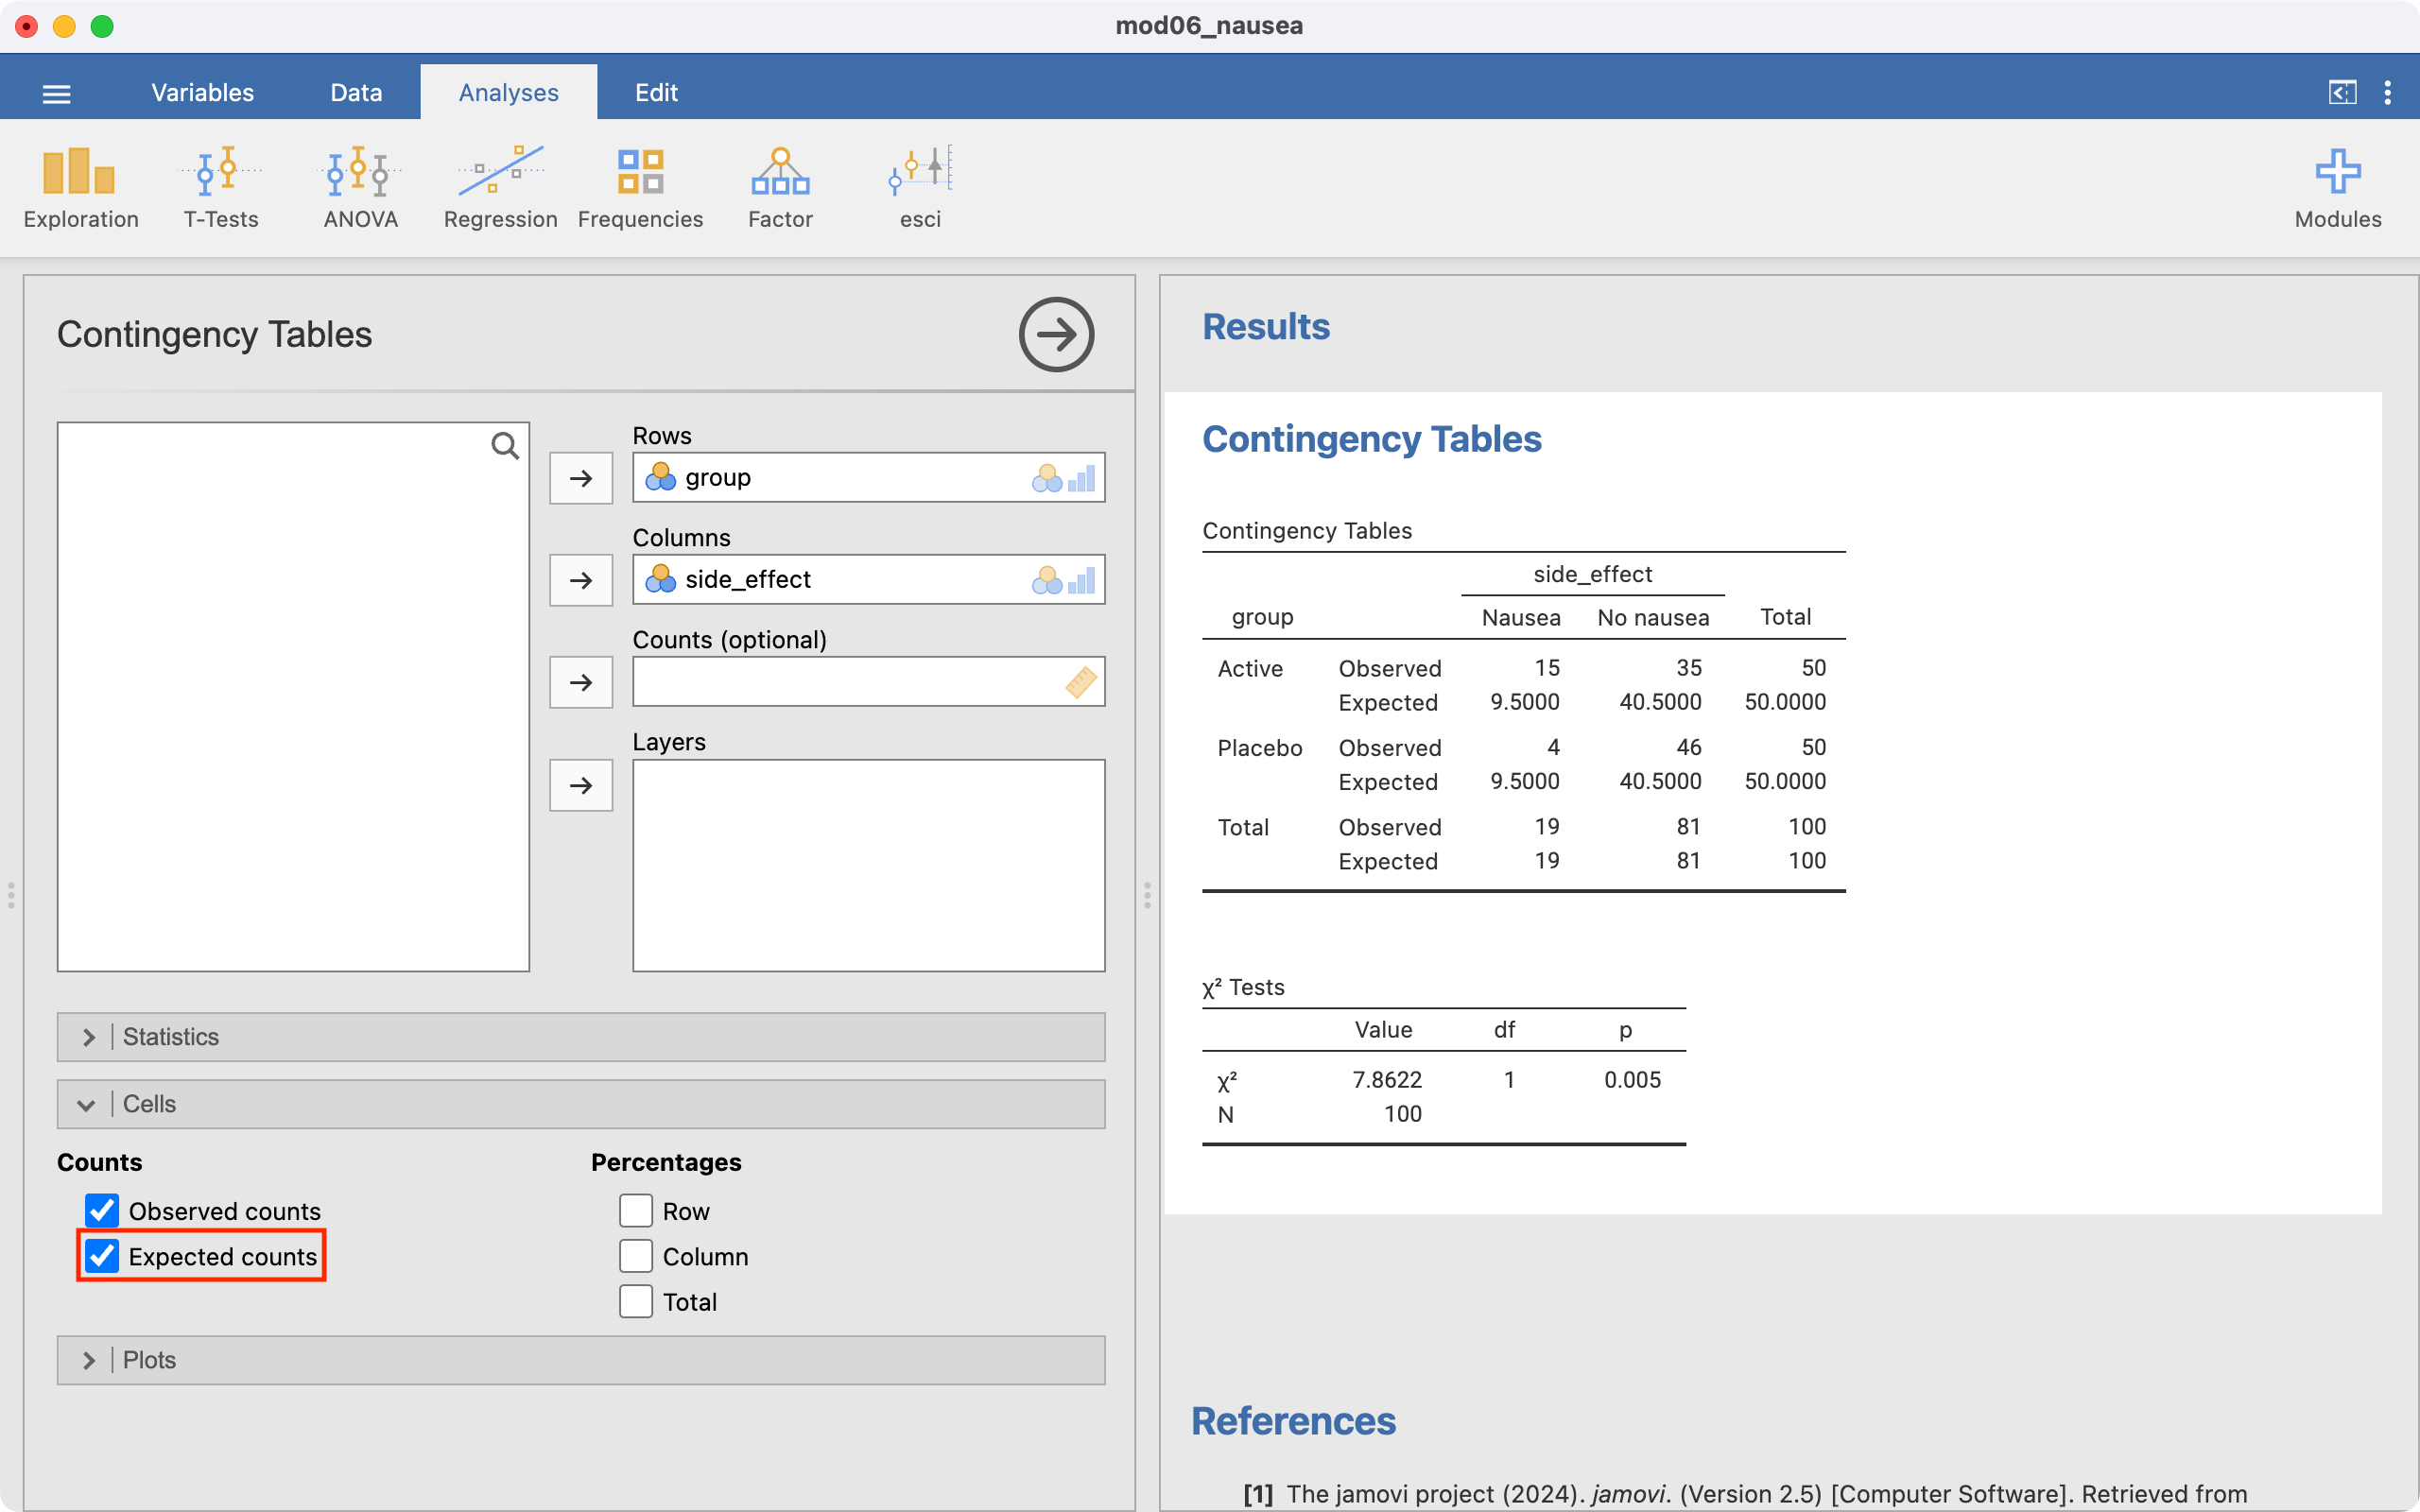
\includegraphics[keepaspectratio]{img/mod07/jamovi/mod07-expected-counts.png}}

After confirming that there are no cells with small expected
frequencies, we can interpret the chi-square test. The last section
reports the chi-squared test statistic which has a value of 7.86 with 1
degree of freedom and a P-value of 0.005.

If there are small values of expected frequencies, Fisher's exact test
can be requested in the \textbf{Statistics} section:

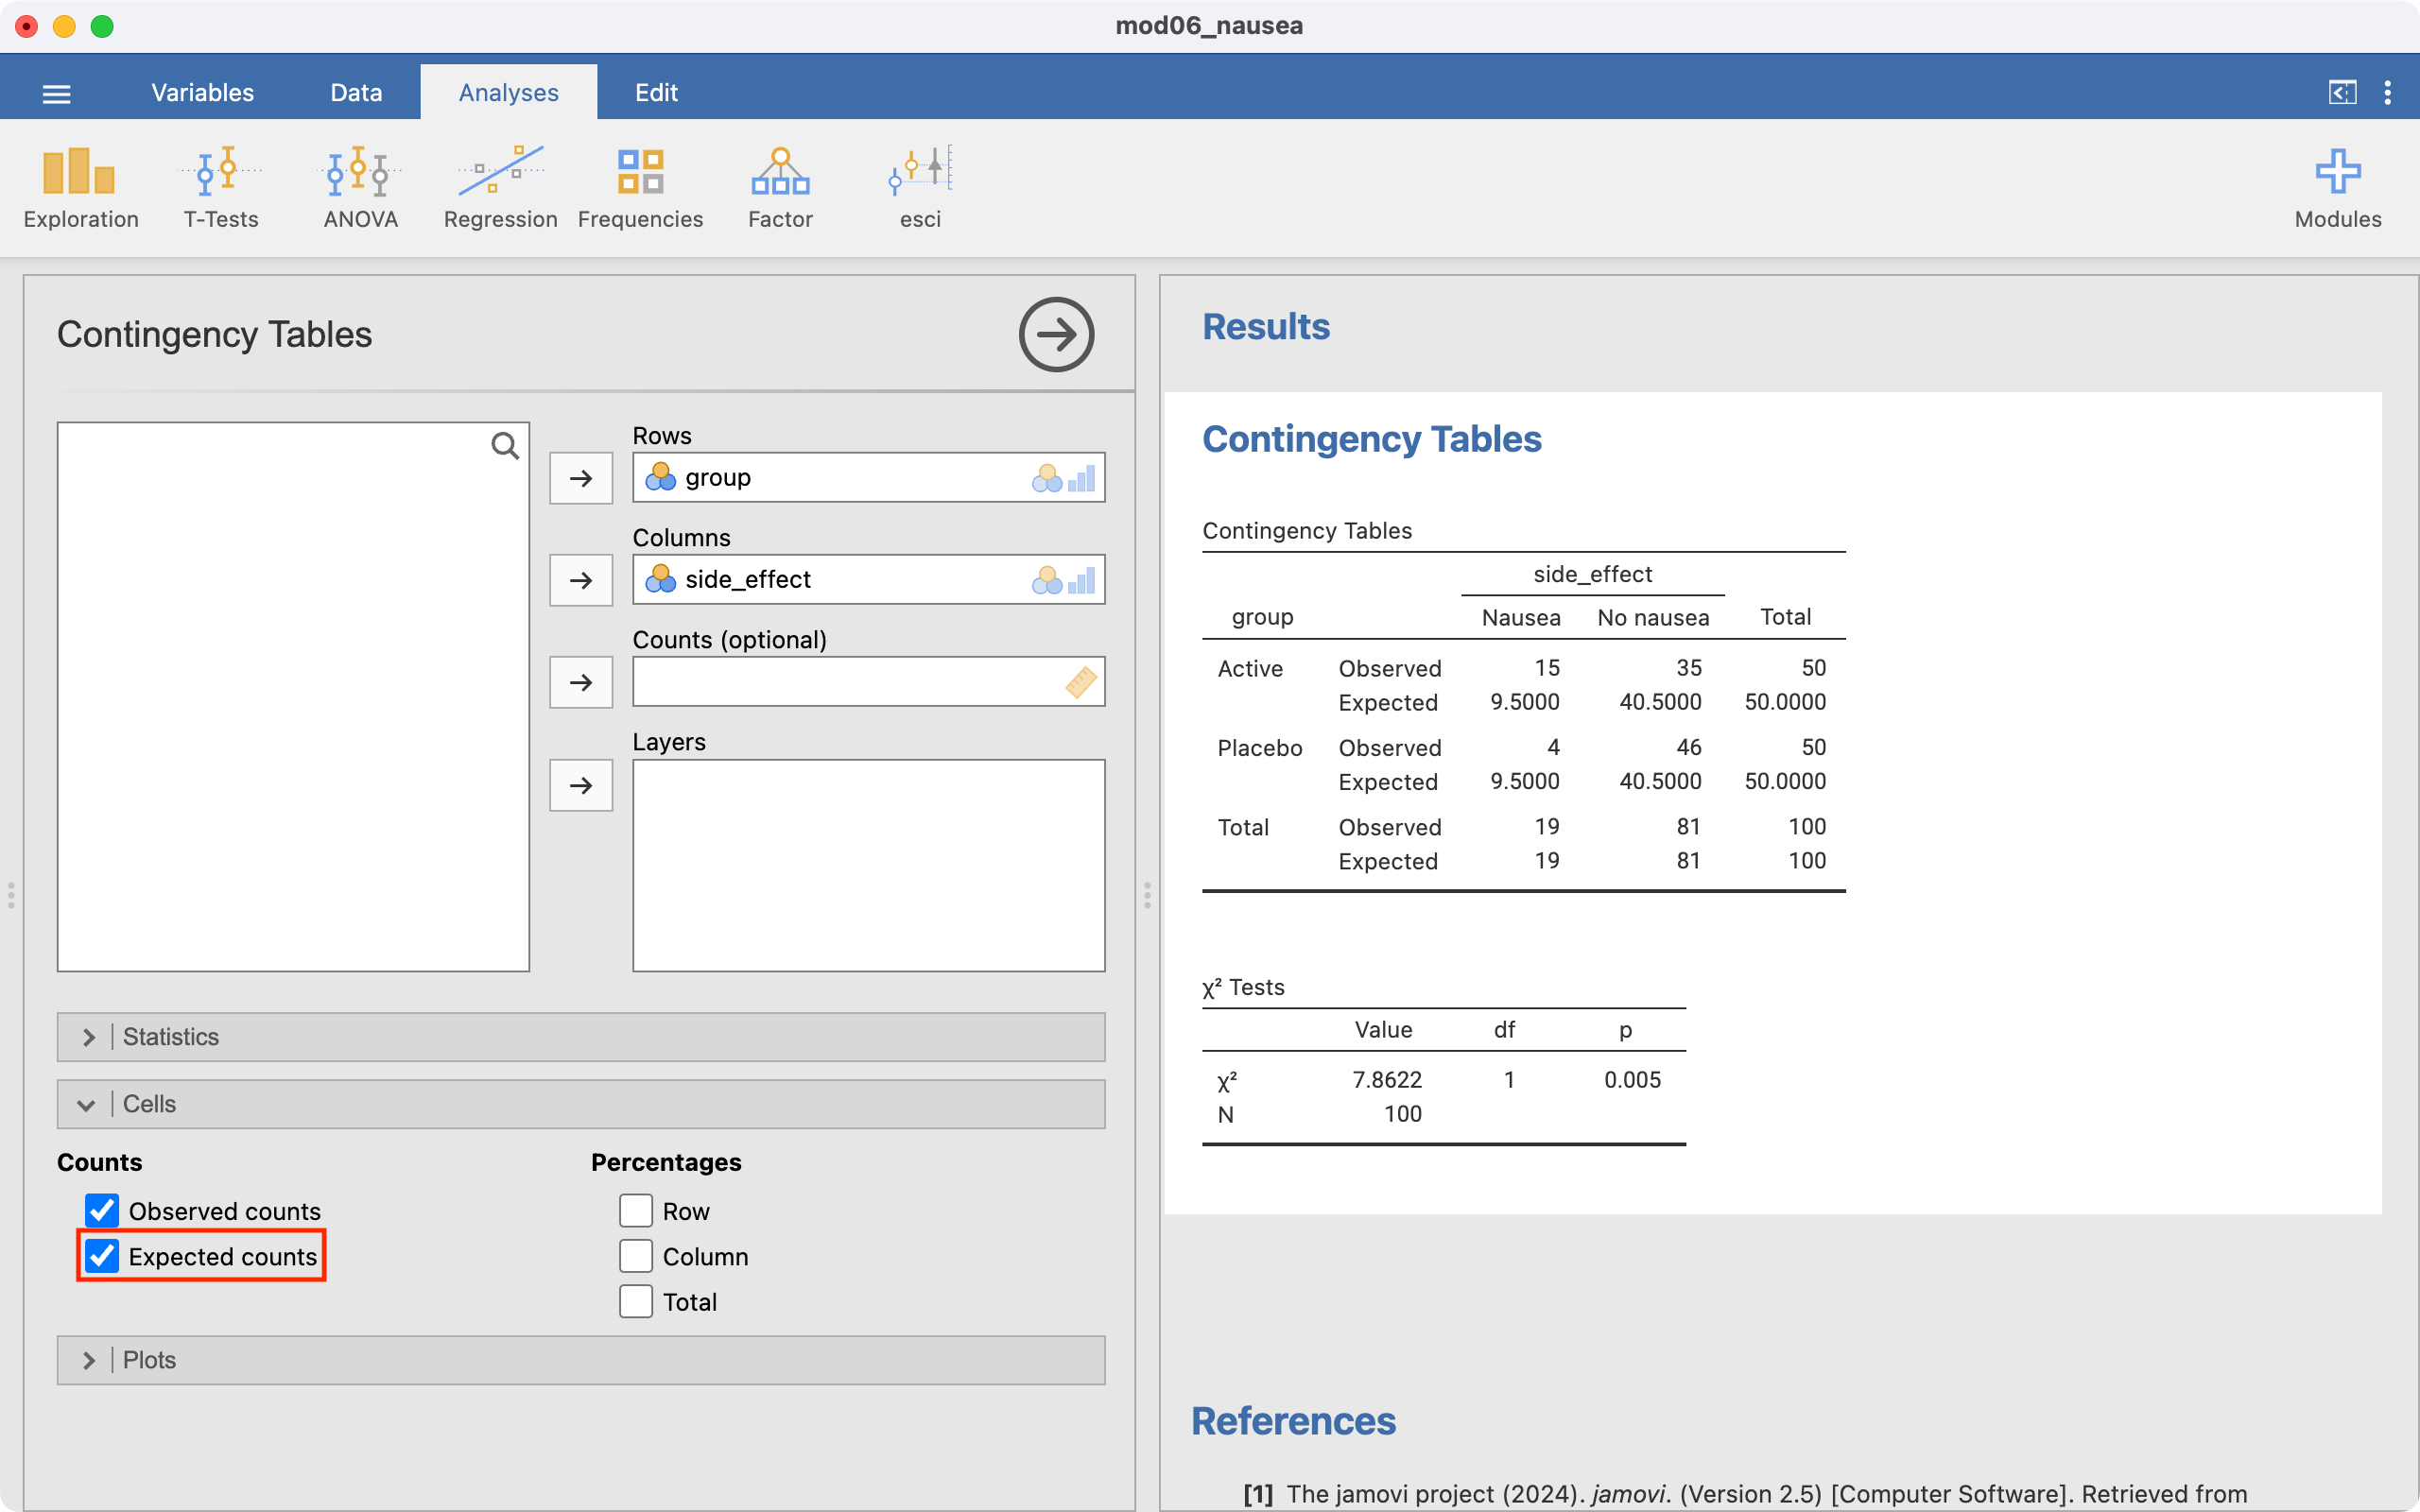
\includegraphics[width=0.5\linewidth,height=\textheight,keepaspectratio]{img/mod07/jamovi/mod07-expected-counts.png}

\section{Pearson's chi-squared test for summarised
data}\label{pearsons-chi-squared-test-for-summarised-data}

When you only have the summarised date (for example, the cross-tabulated
data), you need to enter the summarised data manually as we did in
Module 6. After defining the \textbf{Count variable}, the Pearson
chi-squared test is calculated automatically.

\section{Chi-squared test for tables larger than
2-by-2}\label{chi-squared-test-for-tables-larger-than-2-by-2}

Use the data in \texttt{mod07\_allergy.rds}. We use similar steps as
described above for a 2-by-2 table:

\pandocbounded{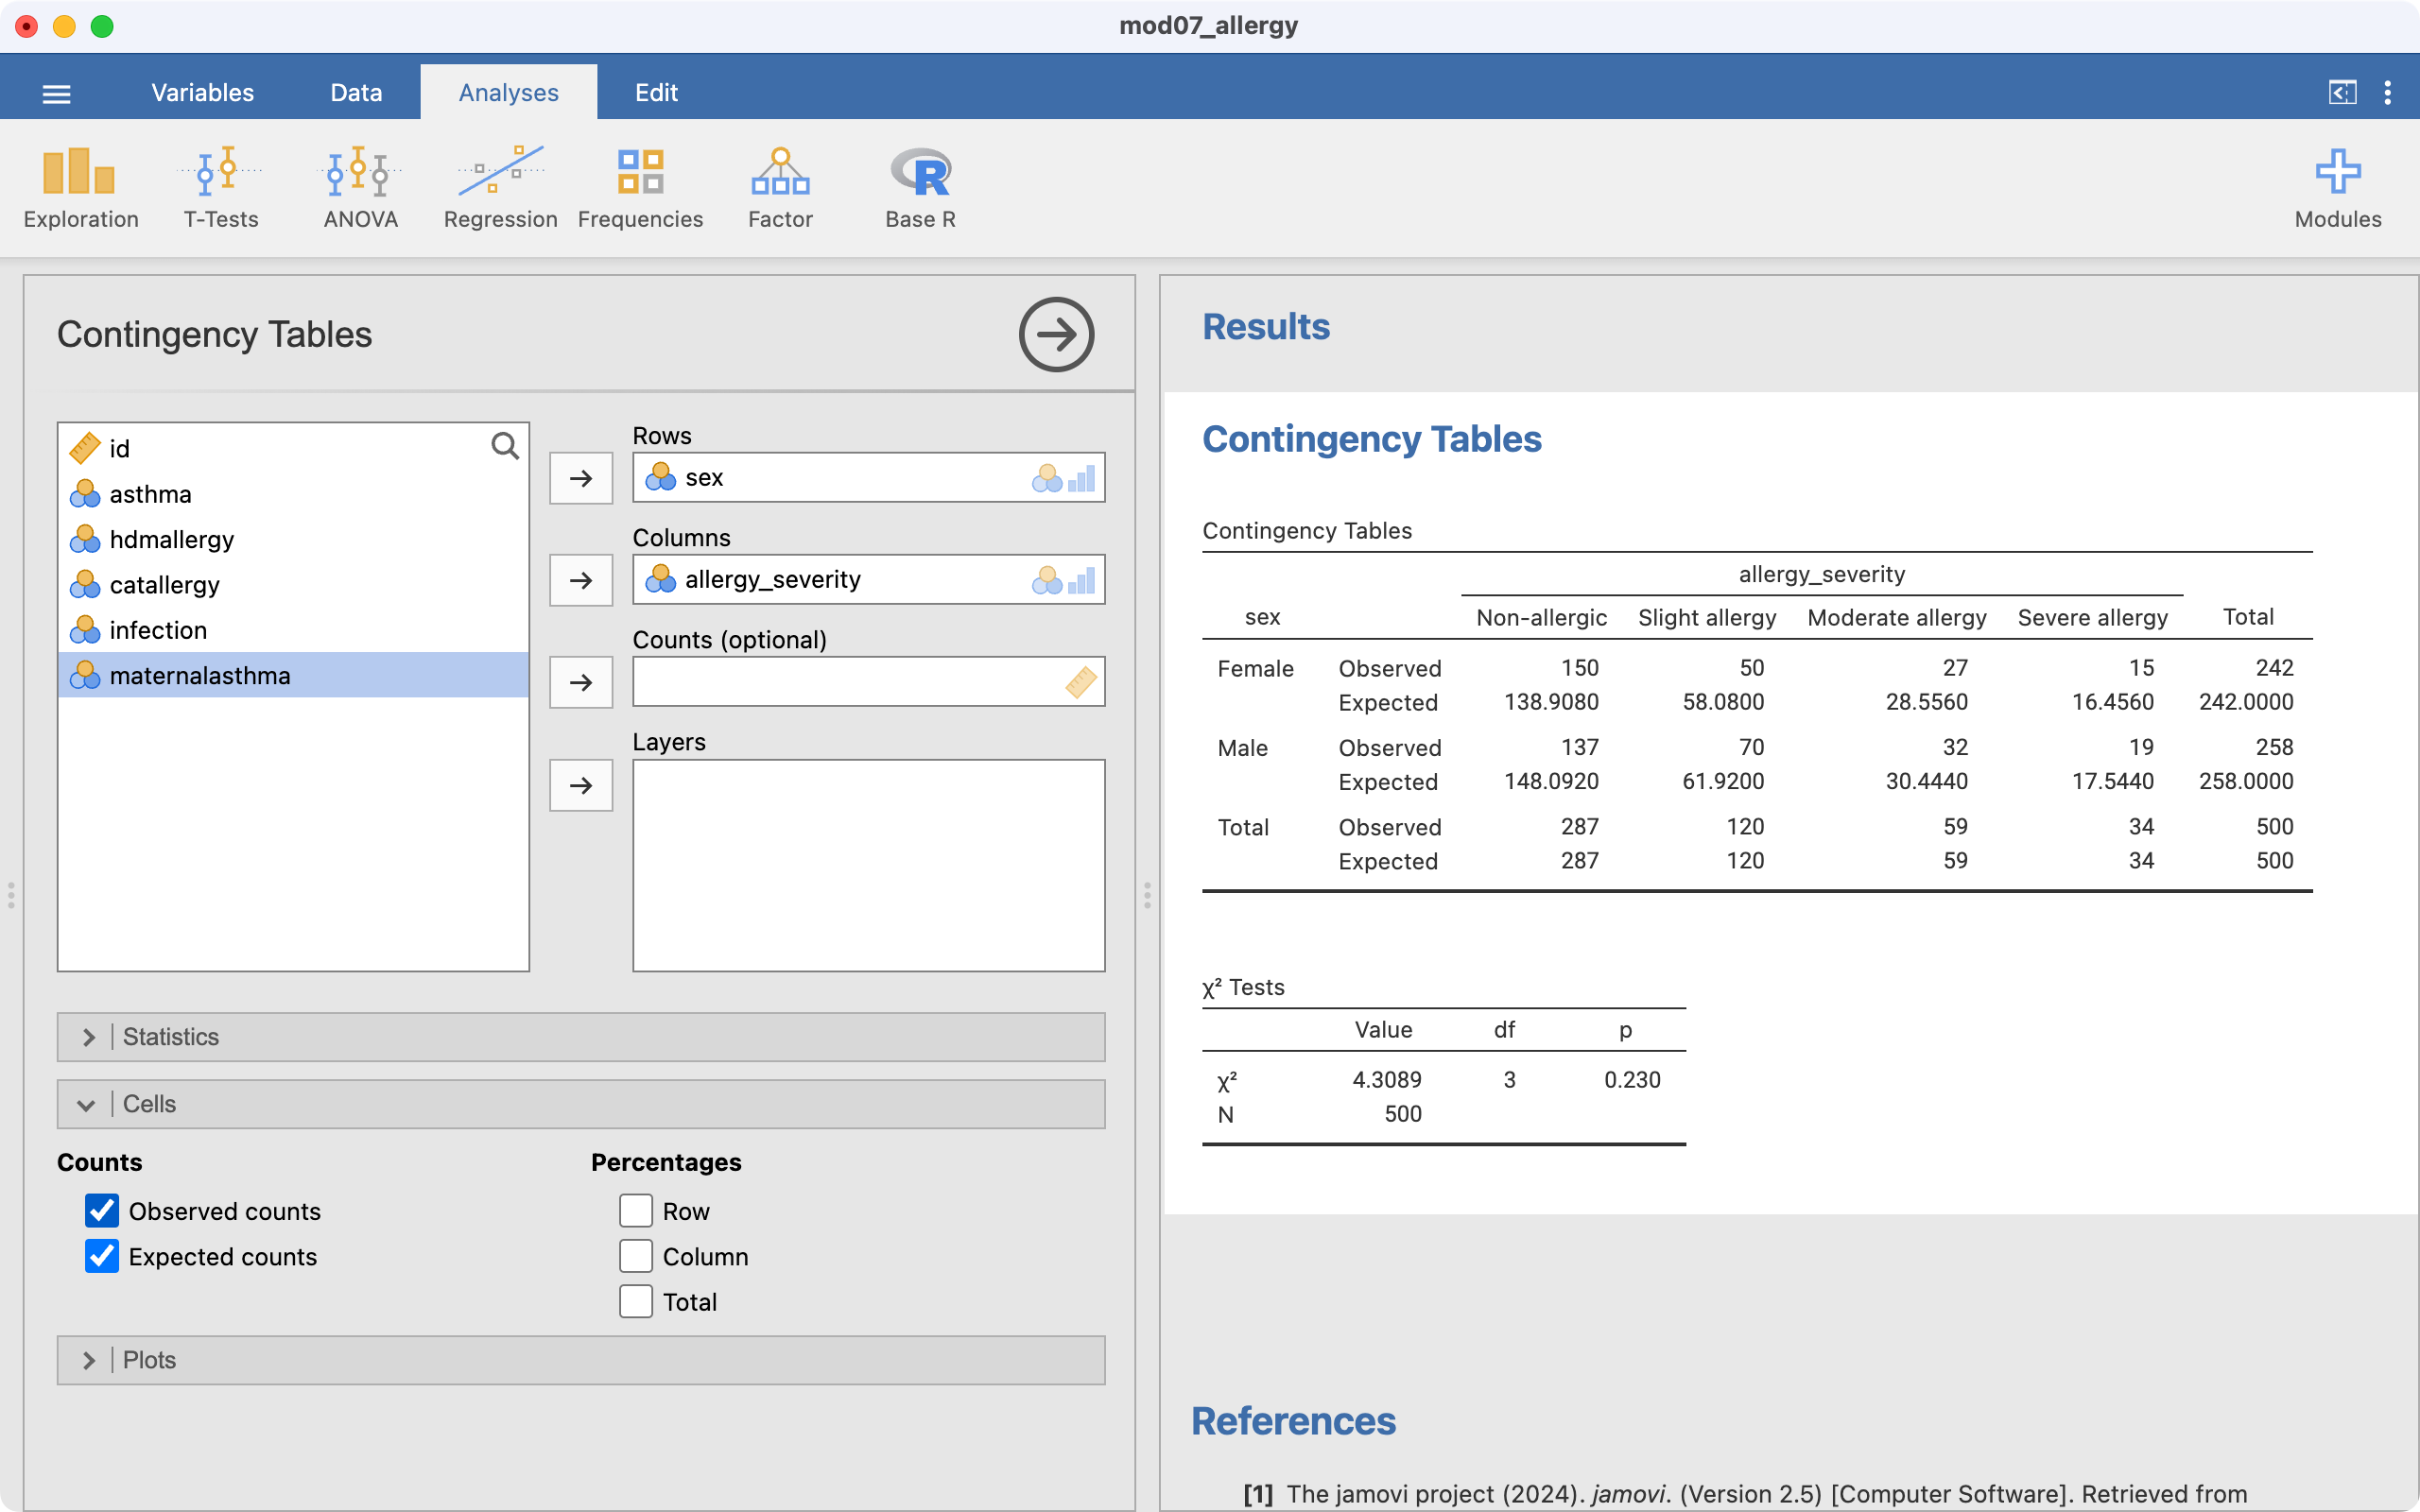
\includegraphics[keepaspectratio]{img/mod07/jamovi/mod07-large-table-expected.png}}

\pandocbounded{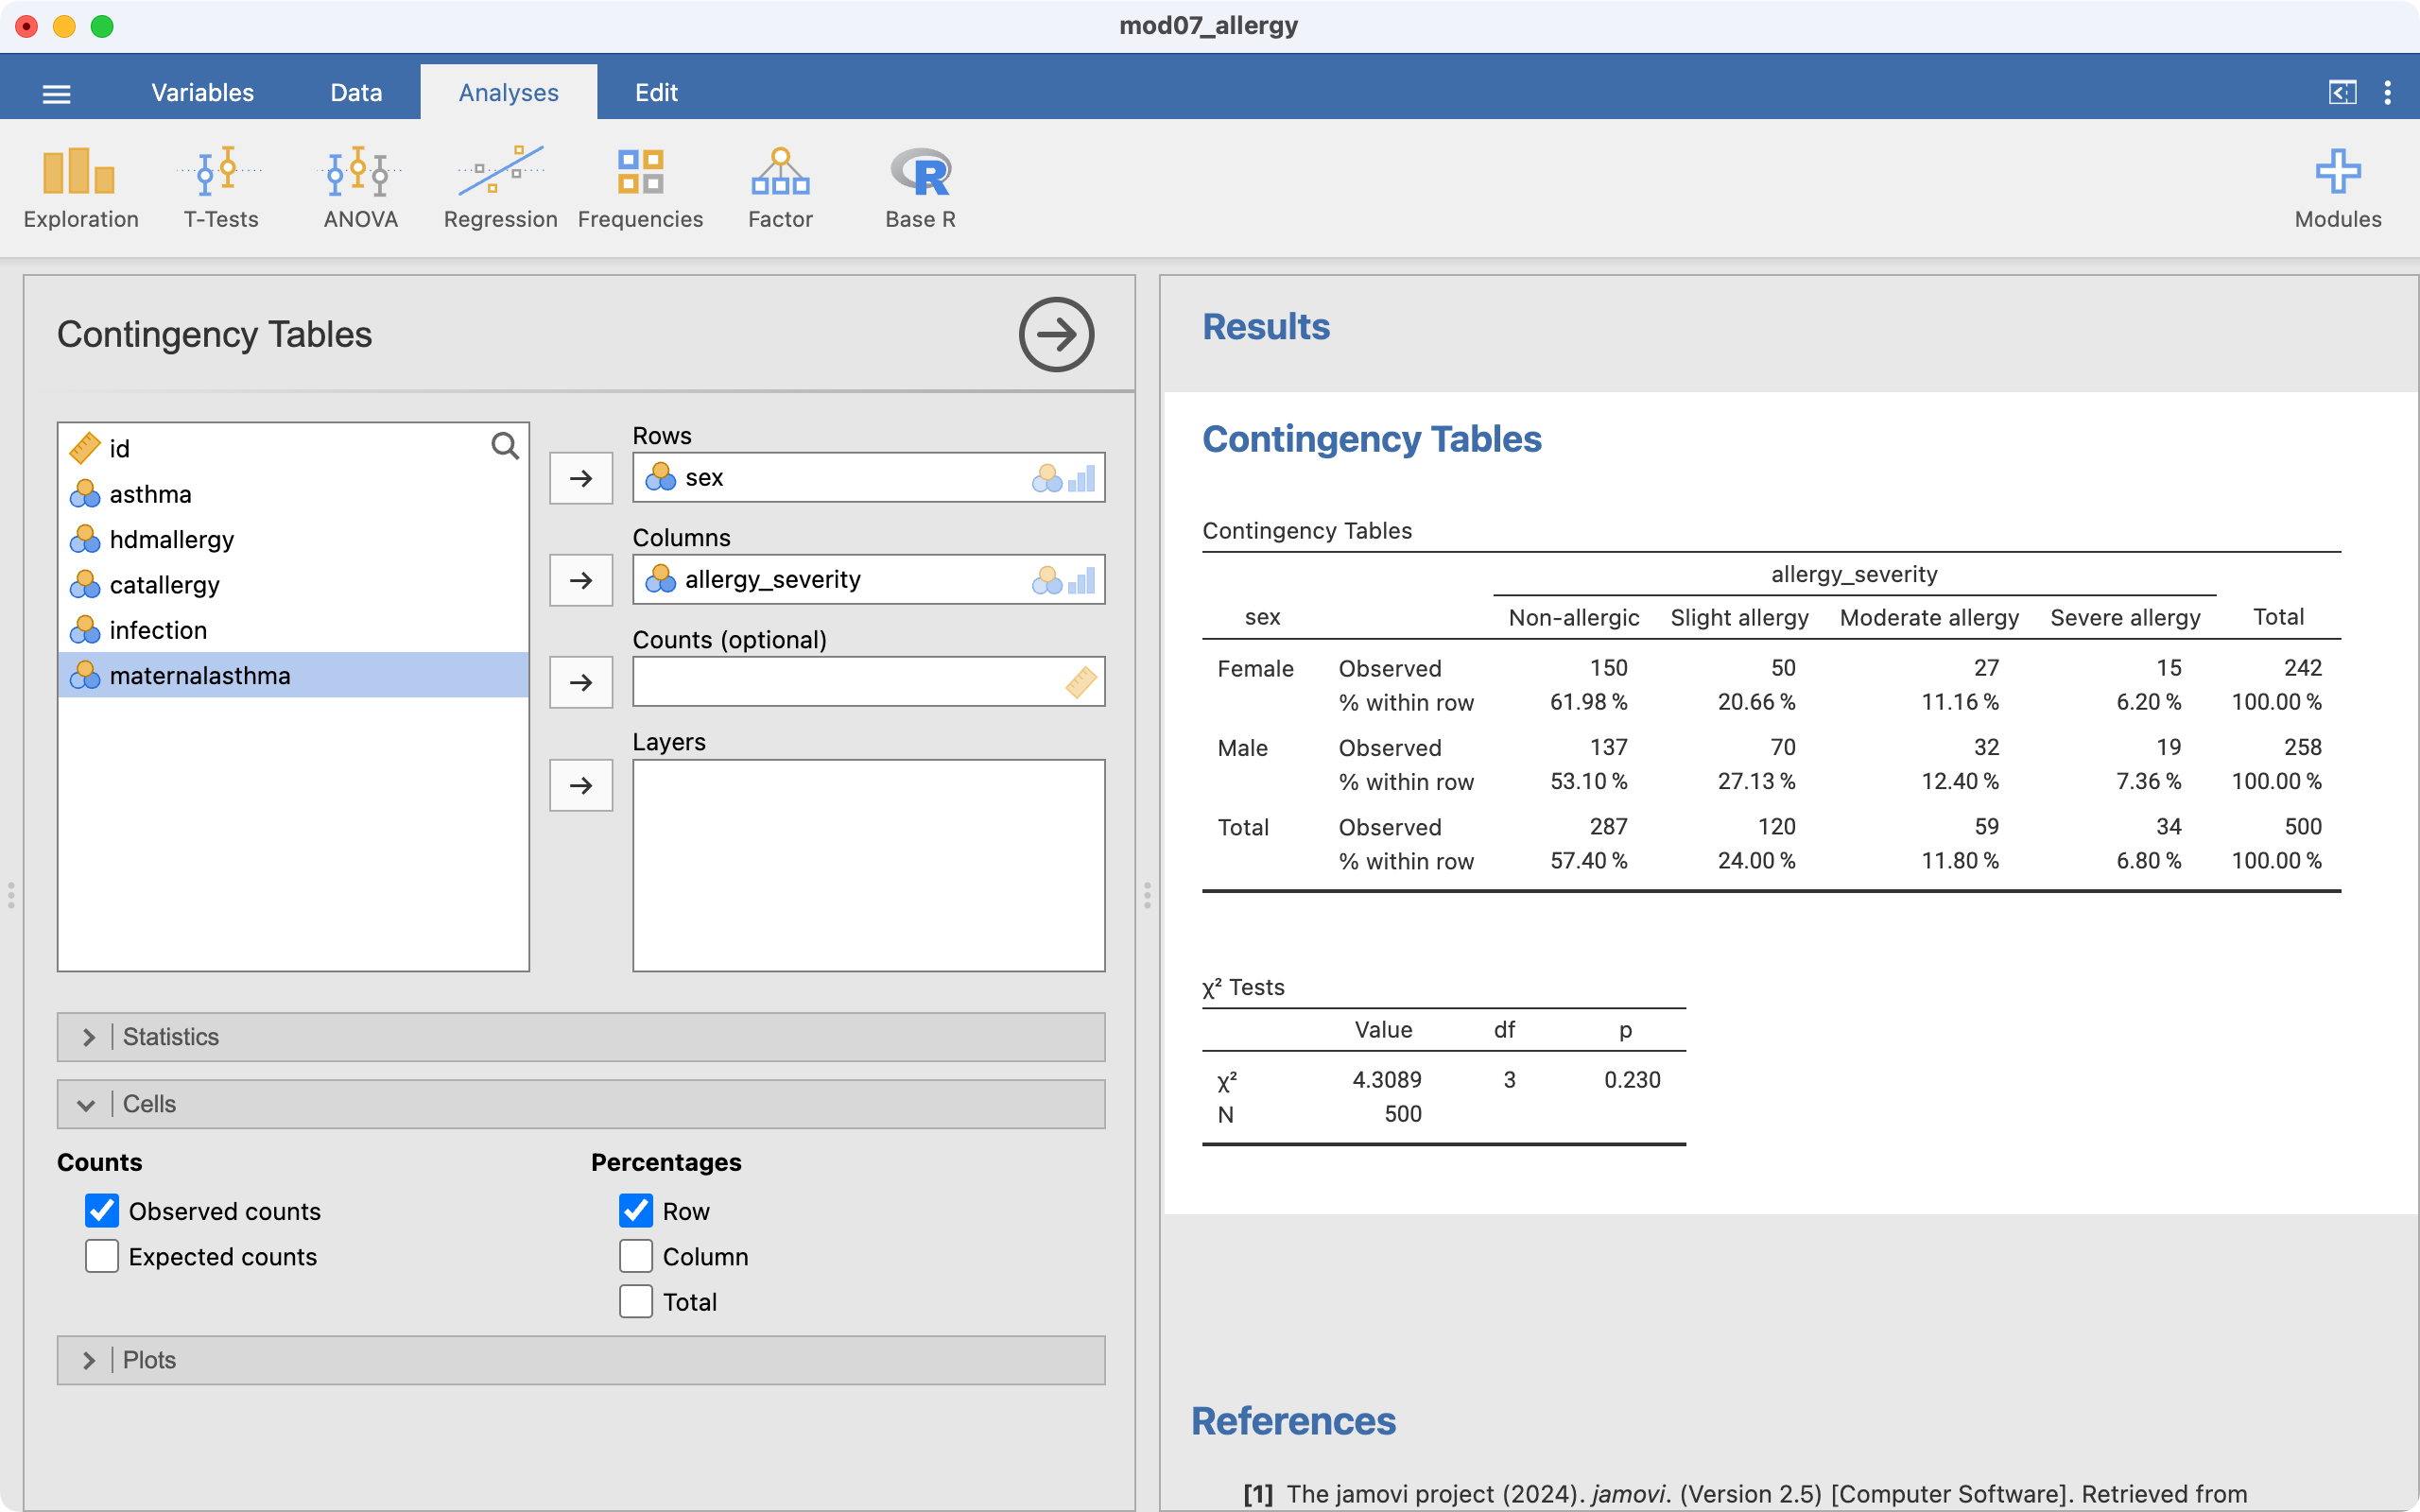
\includegraphics[keepaspectratio]{img/mod07/jamovi/mod07-large-table.png}}

\section{McNemar's test for paired
proportions}\label{mcnemars-test-for-paired-proportions}

To perform this test in jamovi, we will use the dataset
\texttt{mod07\_drug\_response.rds}. As with all 2-by-2 tables, we should
check that the variables are set up with the first level of the variable
being the outcome of interest using \textbf{Data \textgreater{} Setup}:

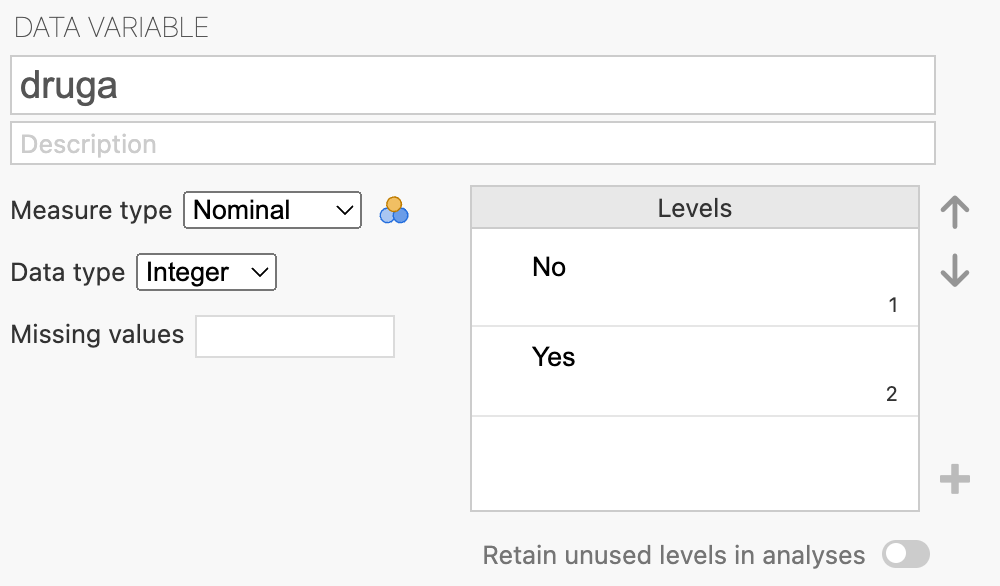
\includegraphics[width=0.5\linewidth,height=\textheight,keepaspectratio]{img/mod07/jamovi/mod07-paired01.png}

Both variables, \texttt{druga} and \texttt{drugb} are set up with ``No''
being the first level. We need to change the order and define ``Yes'' as
the first level (See Module 6 jamovi notes on how to do this):

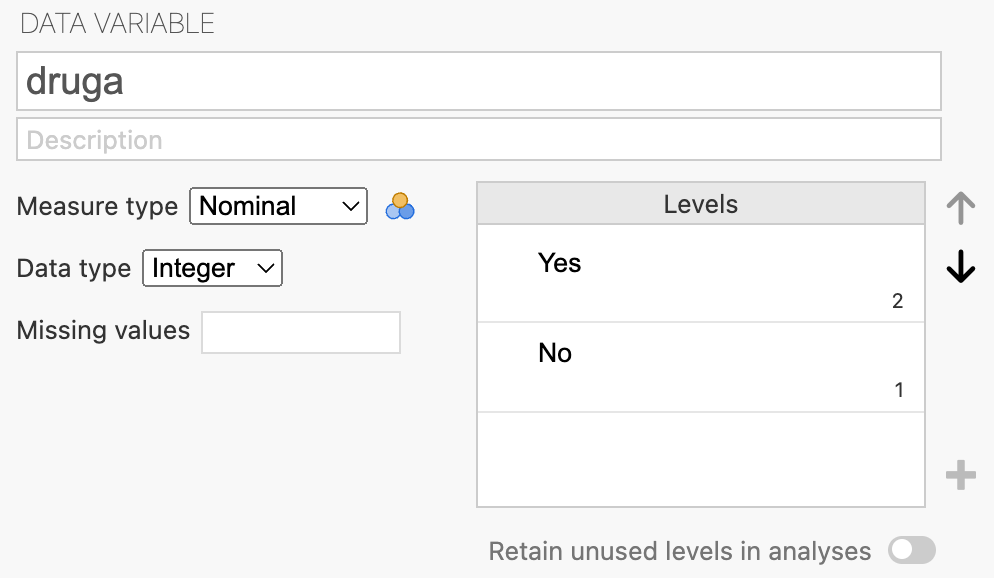
\includegraphics[width=0.5\linewidth,height=\textheight,keepaspectratio]{img/mod07/jamovi/mod07-paired02.png}

The McNemar's test of paired proportions can be conducted at
\textbf{Analyses \textgreater{} Frequencies \textgreater{} Contingency
Tables \textgreater{} Paired Samples \textgreater{} McNemar test}:

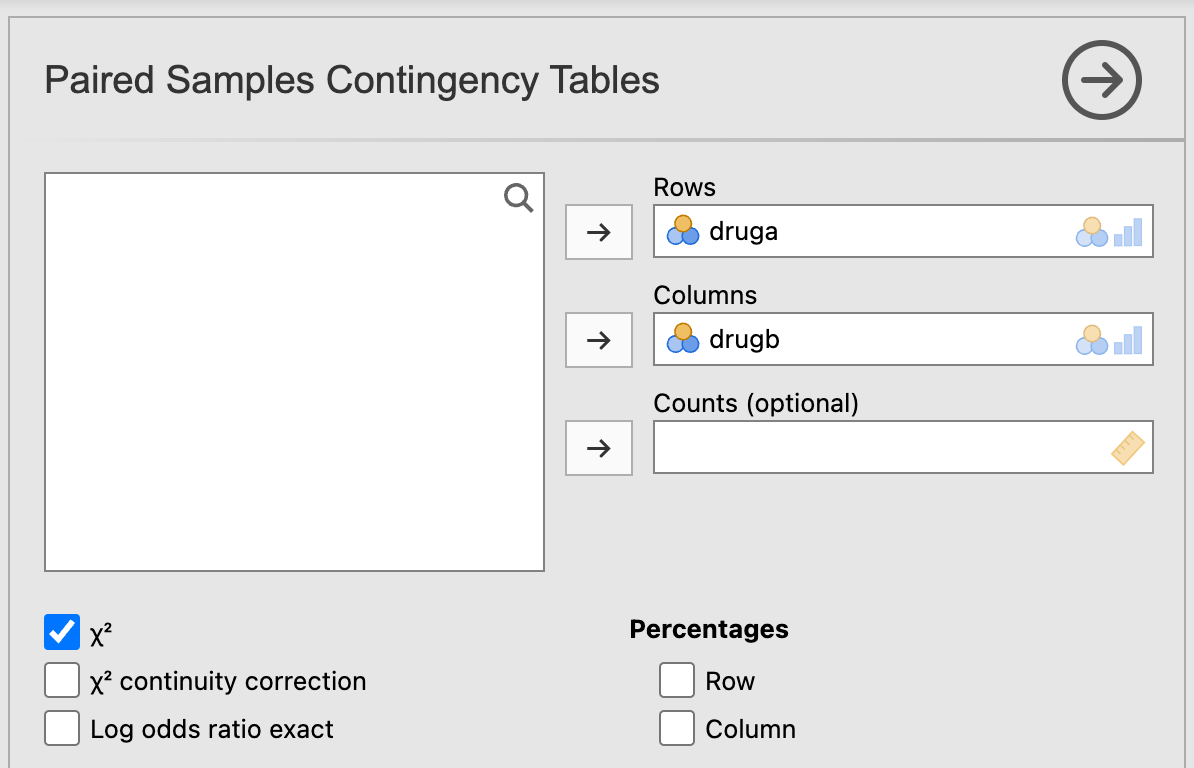
\includegraphics[width=0.5\linewidth,height=\textheight,keepaspectratio]{img/mod07/jamovi/mod07-paired03.png}

Note that jamovi does not currently provide an estimate of the
difference in paired proportions, or a confidence interval for the
difference.

\newpage{}

\bookmarksetup{startatroot}

\chapter*{R notes}\label{r-notes-5}
\addcontentsline{toc}{chapter}{R notes}

\markboth{R notes}{R notes}

\section{Pearson's chi-squared test for individual-level
data}\label{pearsons-chi-squared-test-for-individual-level-data-1}

We will demonstrate how to use R to conduct a Pearson chi-squared test
using Worked Example 7.1.

\begin{Shaded}
\begin{Highlighting}[]
\FunctionTok{library}\NormalTok{(jmv)}
\FunctionTok{library}\NormalTok{(dplyr)}

\NormalTok{nausea }\OtherTok{\textless{}{-}} \FunctionTok{readRDS}\NormalTok{(}\StringTok{"data/examples/mod06\_nausea.rds"}\NormalTok{)}

\FunctionTok{head}\NormalTok{(nausea)}
\end{Highlighting}
\end{Shaded}

\begin{verbatim}
    group side_effect
1 Placebo      Nausea
2 Placebo      Nausea
3 Placebo      Nausea
4 Placebo      Nausea
5 Placebo   No nausea
6 Placebo   No nausea
\end{verbatim}

\begin{Shaded}
\begin{Highlighting}[]
\FunctionTok{str}\NormalTok{(nausea}\SpecialCharTok{$}\NormalTok{group)}
\end{Highlighting}
\end{Shaded}

\begin{verbatim}
 Factor w/ 2 levels "Placebo","Active": 1 1 1 1 1 1 1 1 1 1 ...
 - attr(*, "label")= chr "Group"
\end{verbatim}

\begin{Shaded}
\begin{Highlighting}[]
\FunctionTok{str}\NormalTok{(nausea}\SpecialCharTok{$}\NormalTok{side\_effect)}
\end{Highlighting}
\end{Shaded}

\begin{verbatim}
 Factor w/ 2 levels "No nausea","Nausea": 2 2 2 2 1 1 1 1 1 1 ...
 - attr(*, "label")= chr "Side effect"
\end{verbatim}

The columns \texttt{group} and \texttt{side\_effect} have been entered
as factors, with ``Placebo'' and ``No nausea'' as the first levels. We
should use the \texttt{relevel()} command to re-order the factor levels.

\begin{Shaded}
\begin{Highlighting}[]
\NormalTok{nausea }\OtherTok{\textless{}{-}} \FunctionTok{mutate}\NormalTok{(nausea, }\AttributeTok{group =} \FunctionTok{relevel}\NormalTok{(group, }\AttributeTok{ref =} \StringTok{"Active"}\NormalTok{), }
                         \AttributeTok{side\_effect =} \FunctionTok{relevel}\NormalTok{(side\_effect, }\AttributeTok{ref =} \StringTok{"Nausea"}\NormalTok{))}

\FunctionTok{str}\NormalTok{(nausea}\SpecialCharTok{$}\NormalTok{group)}
\end{Highlighting}
\end{Shaded}

\begin{verbatim}
 Factor w/ 2 levels "Active","Placebo": 2 2 2 2 2 2 2 2 2 2 ...
\end{verbatim}

\begin{Shaded}
\begin{Highlighting}[]
\FunctionTok{str}\NormalTok{(nausea}\SpecialCharTok{$}\NormalTok{side\_effect)}
\end{Highlighting}
\end{Shaded}

\begin{verbatim}
 Factor w/ 2 levels "Nausea","No nausea": 1 1 1 1 2 2 2 2 2 2 ...
\end{verbatim}

After confirming the factors are appropriately defined, we can construct
our 2-by-2 table and view the expected frequencies.

\begin{Shaded}
\begin{Highlighting}[]
\FunctionTok{contTables}\NormalTok{(}
    \AttributeTok{data =}\NormalTok{ nausea,}
    \AttributeTok{rows =}\NormalTok{ group, }\AttributeTok{cols =}\NormalTok{ side\_effect,}
    \AttributeTok{exp =} \ConstantTok{TRUE}
\NormalTok{)}
\end{Highlighting}
\end{Shaded}

\begin{verbatim}

 CONTINGENCY TABLES

 Contingency Tables                                             
 ────────────────────────────────────────────────────────────── 
   group                  Nausea       No nausea    Total       
 ────────────────────────────────────────────────────────────── 
   Active     Observed           15           35           50   
              Expected     9.500000     40.50000     50.00000   
                                                                
   Placebo    Observed            4           46           50   
              Expected     9.500000     40.50000     50.00000   
                                                                
   Total      Observed           19           81          100   
              Expected    19.000000     81.00000    100.00000   
 ────────────────────────────────────────────────────────────── 


 χ² Tests                              
 ───────────────────────────────────── 
         Value       df    p           
 ───────────────────────────────────── 
   χ²    7.862248     1    0.0050478   
   N          100                      
 ───────────────────────────────────── 
\end{verbatim}

After confirming that there are no cells with small expected
frequencies, we can interpret the chi-square test. The last section
reports the chi-squared test statistic which has a value of 7.86 with 1
degree of freedom and a P-value of 0.005.

If there are small values of expected frequencies, Fisher's exact test
can be requested using \texttt{fisher\ =\ TRUE}:

\begin{Shaded}
\begin{Highlighting}[]
\FunctionTok{contTables}\NormalTok{(}
    \AttributeTok{data =}\NormalTok{ nausea,}
    \AttributeTok{rows =}\NormalTok{ group, }\AttributeTok{cols =}\NormalTok{ side\_effect,}
    \AttributeTok{fisher =} \ConstantTok{TRUE}
\NormalTok{)}
\end{Highlighting}
\end{Shaded}

\begin{verbatim}

 CONTINGENCY TABLES

 Contingency Tables                          
 ─────────────────────────────────────────── 
   group      Nausea    No nausea    Total   
 ─────────────────────────────────────────── 
   Active         15           35       50   
   Placebo         4           46       50   
   Total          19           81      100   
 ─────────────────────────────────────────── 


 χ² Tests                                               
 ────────────────────────────────────────────────────── 
                          Value       df    p           
 ────────────────────────────────────────────────────── 
   χ²                     7.862248     1    0.0050478   
   Fisher's exact test                      0.0094886   
   N                           100                      
 ────────────────────────────────────────────────────── 
\end{verbatim}

\section{Pearson's chi-squared test for summarised
data}\label{pearsons-chi-squared-test-for-summarised-data-1}

When you only have the summarised date (for example, the cross-tabulated
data), you need to enter the summarised data manually. As we did in
Module 6, the 2-by-2 table can be entered as four lines of data:

\begin{Shaded}
\begin{Highlighting}[]
\NormalTok{drug\_aggregated }\OtherTok{\textless{}{-}} \FunctionTok{data.frame}\NormalTok{(}
    \AttributeTok{group =} \FunctionTok{c}\NormalTok{(}\StringTok{"Active"}\NormalTok{, }\StringTok{"Active"}\NormalTok{, }\StringTok{"Placebo"}\NormalTok{, }\StringTok{"Placebo"}\NormalTok{),}
    \AttributeTok{side\_effect =} \FunctionTok{c}\NormalTok{(}\StringTok{"Nausea"}\NormalTok{, }\StringTok{"No nausea"}\NormalTok{, }\StringTok{"Nausea"}\NormalTok{, }\StringTok{"No nausea"}\NormalTok{),}
    \AttributeTok{n =} \FunctionTok{c}\NormalTok{(}\DecValTok{15}\NormalTok{, }\DecValTok{35}\NormalTok{, }\DecValTok{4}\NormalTok{, }\DecValTok{46}\NormalTok{)}
\NormalTok{)}
\end{Highlighting}
\end{Shaded}

The \texttt{contTables()} function is used in the usual way, specifying
\texttt{count=n}.

\section{Chi-squared test for tables larger than
2-by-2}\label{chi-squared-test-for-tables-larger-than-2-by-2-1}

Use the data in \texttt{mod07\_allergy.rds}. We use similar steps as
described above for a 2-by-2 table.

\begin{Shaded}
\begin{Highlighting}[]
\NormalTok{allergy }\OtherTok{\textless{}{-}} \FunctionTok{readRDS}\NormalTok{(}\StringTok{"data/examples/mod07\_allergy.rds"}\NormalTok{)}

\FunctionTok{head}\NormalTok{(allergy)}
\end{Highlighting}
\end{Shaded}

\begin{verbatim}
  id asthma hdmallergy catallergy infection    sex maternalasthma
1  1     No        Yes         No       Yes Female             No
2  2    Yes         No         No        No Female             No
3  3    Yes         No         No        No Female             No
4  4     No         No         No        No   Male             No
5  4    Yes        Yes        Yes        No Female             No
6  5    Yes        Yes        Yes        No Female             No
  allergy_severity
1 Moderate allergy
2     Non-allergic
3     Non-allergic
4     Non-allergic
5 Moderate allergy
6 Moderate allergy
\end{verbatim}

\begin{Shaded}
\begin{Highlighting}[]
\FunctionTok{contTables}\NormalTok{(}
    \AttributeTok{data =}\NormalTok{ allergy,}
    \AttributeTok{rows =}\NormalTok{ allergy\_severity, }\AttributeTok{cols =}\NormalTok{ sex,}
    \AttributeTok{pcCol =} \ConstantTok{TRUE}
\NormalTok{)}
\end{Highlighting}
\end{Shaded}

\begin{verbatim}

 CONTINGENCY TABLES

 Contingency Tables                                                             
 ────────────────────────────────────────────────────────────────────────────── 
   allergy_severity                       Female       Male         Total       
 ────────────────────────────────────────────────────────────────────────────── 
   Non-allergic        Observed                 150          137          287   
                       % within column     61.98347     53.10078     57.40000   
                                                                                
   Slight allergy      Observed                  50           70          120   
                       % within column     20.66116     27.13178     24.00000   
                                                                                
   Moderate allergy    Observed                  27           32           59   
                       % within column     11.15702     12.40310     11.80000   
                                                                                
   Severe allergy      Observed                  15           19           34   
                       % within column      6.19835      7.36434      6.80000   
                                                                                
   Total               Observed                 242          258          500   
                       % within column    100.00000    100.00000    100.00000   
 ────────────────────────────────────────────────────────────────────────────── 


 χ² Tests                              
 ───────────────────────────────────── 
         Value       df    p           
 ───────────────────────────────────── 
   χ²    4.308913     3    0.2299813   
   N          500                      
 ───────────────────────────────────── 
\end{verbatim}

\section{McNemar's test for paired
proportions}\label{mcnemars-test-for-paired-proportions-1}

To perform this test in R, we will use the dataset
\texttt{mod07\_drug\_response.rds}.

\begin{Shaded}
\begin{Highlighting}[]
\NormalTok{drug }\OtherTok{\textless{}{-}} \FunctionTok{readRDS}\NormalTok{(}\StringTok{"data/examples/mod07\_drug\_response.rds"}\NormalTok{)}

\FunctionTok{head}\NormalTok{(drug)}
\end{Highlighting}
\end{Shaded}

\begin{verbatim}
  druga drugb
1   Yes   Yes
2   Yes   Yes
3   Yes   Yes
4   Yes   Yes
5   Yes   Yes
6   Yes   Yes
\end{verbatim}

As usual, we should check that the variables being tabulated are
factors, with the first level of the factor being the outcome of
interest.

\begin{Shaded}
\begin{Highlighting}[]
\FunctionTok{str}\NormalTok{(drug}\SpecialCharTok{$}\NormalTok{druga)}
\end{Highlighting}
\end{Shaded}

\begin{verbatim}
 Factor w/ 2 levels "No","Yes": 2 2 2 2 2 2 2 2 2 2 ...
 - attr(*, "label")= chr "Response to Drug A"
\end{verbatim}

\begin{Shaded}
\begin{Highlighting}[]
\FunctionTok{str}\NormalTok{(drug}\SpecialCharTok{$}\NormalTok{drugb)}
\end{Highlighting}
\end{Shaded}

\begin{verbatim}
 Factor w/ 2 levels "No","Yes": 2 2 2 2 2 2 2 2 2 2 ...
 - attr(*, "label")= chr "Response to Drug B"
\end{verbatim}

Here we see that the first level of the factor is ``No'' - we need to
use the \texttt{relevel()} function to re-order the levels so ``Yes'' is
the first level:

\begin{Shaded}
\begin{Highlighting}[]
\NormalTok{drug }\OtherTok{\textless{}{-}} \FunctionTok{mutate}\NormalTok{(drug, }\AttributeTok{druga =} \FunctionTok{relevel}\NormalTok{(druga, }\AttributeTok{ref =} \StringTok{"Yes"}\NormalTok{),}
                     \AttributeTok{drugb =} \FunctionTok{relevel}\NormalTok{(drugb, }\AttributeTok{ref =} \StringTok{"Yes"}\NormalTok{))}

\FunctionTok{str}\NormalTok{(drug}\SpecialCharTok{$}\NormalTok{druga)}
\end{Highlighting}
\end{Shaded}

\begin{verbatim}
 Factor w/ 2 levels "Yes","No": 1 1 1 1 1 1 1 1 1 1 ...
\end{verbatim}

\begin{Shaded}
\begin{Highlighting}[]
\FunctionTok{str}\NormalTok{(drug}\SpecialCharTok{$}\NormalTok{drugb)}
\end{Highlighting}
\end{Shaded}

\begin{verbatim}
 Factor w/ 2 levels "Yes","No": 1 1 1 1 1 1 1 1 1 1 ...
\end{verbatim}

We can use the \texttt{contTablesPaired()} function within the
\texttt{jmv} library to conduct McNemar's test of paired proportions:

\begin{Shaded}
\begin{Highlighting}[]
\FunctionTok{contTablesPaired}\NormalTok{(}\AttributeTok{data =}\NormalTok{ drug, }\AttributeTok{rows =}\NormalTok{ druga, }\AttributeTok{cols =}\NormalTok{ drugb)}
\end{Highlighting}
\end{Shaded}

\begin{verbatim}

 PAIRED SAMPLES CONTINGENCY TABLES

 Contingency Tables              
 ─────────────────────────────── 
   druga    Yes    No    Total   
 ─────────────────────────────── 
   Yes       21    20       41   
   No        14     5       19   
   Total     35    25       60   
 ─────────────────────────────── 


 McNemar Test                          
 ───────────────────────────────────── 
         Value       df    p           
 ───────────────────────────────────── 
   χ²    1.058824     1    0.3034837   
   N           60                      
 ───────────────────────────────────── 
\end{verbatim}

Note that \texttt{contTablesPaired()} does not calculate an exact
P-value.

To estimate the proportion in each of the paired samples, its
difference, and the 95\% confidence interval of the difference, we can
use the \texttt{mcNemarDiff()} function which can be downloaded
\href{https://gist.githubusercontent.com/timothydobbins/525d25271b04b2ea72aae70c4aac8b01/raw/6b69f5b229d50daeac4c2f4cf4331e88b0c65717/mcNemarDiff.R}{here}.

\begin{Shaded}
\begin{Highlighting}[]
\DocumentationTok{\#\#\# Copied from gist.githubusercontent.com}
\NormalTok{mcNemarDiff }\OtherTok{\textless{}{-}} \ControlFlowTok{function}\NormalTok{(data, var1, var2, }\AttributeTok{digits =} \DecValTok{3}\NormalTok{) \{}
    \ControlFlowTok{if}\NormalTok{ (}\SpecialCharTok{!}\FunctionTok{requireNamespace}\NormalTok{(}\StringTok{"epibasix"}\NormalTok{, }\AttributeTok{quietly =} \ConstantTok{TRUE}\NormalTok{)) \{}
        \FunctionTok{stop}\NormalTok{(}\StringTok{"This function requires epibasix to be installed"}\NormalTok{)}
\NormalTok{    \}}

\NormalTok{    tab }\OtherTok{\textless{}{-}} \FunctionTok{table}\NormalTok{(data[[var1]], data[[var2]])}
\NormalTok{    p1 }\OtherTok{\textless{}{-}}\NormalTok{ (tab[}\DecValTok{1}\NormalTok{, }\DecValTok{1}\NormalTok{] }\SpecialCharTok{+}\NormalTok{ tab[}\DecValTok{1}\NormalTok{, }\DecValTok{2}\NormalTok{]) }\SpecialCharTok{/} \FunctionTok{sum}\NormalTok{(tab)}
\NormalTok{    p2 }\OtherTok{\textless{}{-}}\NormalTok{ (tab[}\DecValTok{1}\NormalTok{, }\DecValTok{1}\NormalTok{] }\SpecialCharTok{+}\NormalTok{ tab[}\DecValTok{2}\NormalTok{, }\DecValTok{1}\NormalTok{]) }\SpecialCharTok{/} \FunctionTok{sum}\NormalTok{(tab)}
\NormalTok{    pd }\OtherTok{\textless{}{-}}\NormalTok{ epibasix}\SpecialCharTok{::}\FunctionTok{mcNemar}\NormalTok{(tab)}\SpecialCharTok{$}\NormalTok{rd}
\NormalTok{    pd.cil }\OtherTok{\textless{}{-}}\NormalTok{ epibasix}\SpecialCharTok{::}\FunctionTok{mcNemar}\NormalTok{(tab)}\SpecialCharTok{$}\NormalTok{rd.CIL}
\NormalTok{    pd.ciu }\OtherTok{\textless{}{-}}\NormalTok{ epibasix}\SpecialCharTok{::}\FunctionTok{mcNemar}\NormalTok{(tab)}\SpecialCharTok{$}\NormalTok{rd.CIU}
    \FunctionTok{print}\NormalTok{(}\FunctionTok{paste0}\NormalTok{(}
        \StringTok{"Proportion 1: "}\NormalTok{,}
        \FunctionTok{format}\NormalTok{(}\FunctionTok{round}\NormalTok{(p1, }\AttributeTok{digits =}\NormalTok{ digits), }\AttributeTok{nsmall =}\NormalTok{ digits),}
        \StringTok{"; Proportion 2: "}\NormalTok{, }\FunctionTok{format}\NormalTok{(}\FunctionTok{round}\NormalTok{(p2, }\AttributeTok{digits =}\NormalTok{ digits), }\AttributeTok{nsmall =}\NormalTok{ digits)}
\NormalTok{    ))}
    \FunctionTok{print}\NormalTok{(}\FunctionTok{paste0}\NormalTok{(}
        \StringTok{"Difference in paired proportions: "}\NormalTok{,}
        \FunctionTok{format}\NormalTok{(}\FunctionTok{round}\NormalTok{(pd, }\AttributeTok{digits =}\NormalTok{ digits), }\AttributeTok{nsmall =}\NormalTok{ digits),}
        \StringTok{"; 95\% CI: "}\NormalTok{, }\FunctionTok{format}\NormalTok{(}\FunctionTok{round}\NormalTok{(pd.cil, }\AttributeTok{digits =}\NormalTok{ digits), }\AttributeTok{nsmall =}\NormalTok{ digits),}
        \StringTok{" to "}\NormalTok{, }\FunctionTok{format}\NormalTok{(}\FunctionTok{round}\NormalTok{(pd.ciu, }\AttributeTok{digits =}\NormalTok{ digits), }\AttributeTok{nsmall =}\NormalTok{ digits)}
\NormalTok{    ))}
\NormalTok{\}}
\DocumentationTok{\#\#\# End copy}

\FunctionTok{mcNemarDiff}\NormalTok{(}\AttributeTok{data =}\NormalTok{ drug, }\AttributeTok{var1 =} \StringTok{"druga"}\NormalTok{, }\AttributeTok{var2 =} \StringTok{"drugb"}\NormalTok{, }\AttributeTok{digits =} \DecValTok{2}\NormalTok{)}
\end{Highlighting}
\end{Shaded}

\begin{verbatim}
[1] "Proportion 1: 0.68; Proportion 2: 0.58"
[1] "Difference in paired proportions: 0.10; 95% CI: -0.11 to 0.31"
\end{verbatim}

In this study of 60 participants, where each participant received both
drugs, 41 (68\%) responded to Drug A and 35 (58\%) responded to Drug B.
The difference in the proportions responding is estimated as 10\% (95\%
CI -11\% to 31\%). There is no evidence that the response differed
between the two drugs (McNemar's chi-squared = 1.06 with 1df, P=0.30).

\newpage{}

\bookmarksetup{startatroot}

\chapter*{Activities}\label{activities-6}
\addcontentsline{toc}{chapter}{Activities}

\markboth{Activities}{Activities}

\subsection*{Activity 7.1}\label{activity-7.1}
\addcontentsline{toc}{subsection}{Activity 7.1}

This activity continues from Activity 6.2, where a survey was conducted
of a random sample of 514 upper primary school children to measure the
prevalence of asthma. Use the dataset \texttt{Activity\_6.2.rds} to
investigate whether there is a gender difference in the prevalence of
asthma.

\subsection*{Activity 7.2}\label{activity-7.2}
\addcontentsline{toc}{subsection}{Activity 7.2}

This activity continues from Activity 6.5, a study to determine the
cause of mortality where 89 people were followed up for 5 years. The
file \texttt{Activity\_7.2.rds} summarise 5-year mortality (the outcome)
for 89 people who did or did not have a heart attack (the exposure). The
data are entered as:

\begin{itemize}
\tightlist
\item
  heart\_attack: Heart attack status: 1=No, 2=Yes
\item
  mortality: 5-year mortality; 1=No, 2=Yes
\end{itemize}

Analyse these data to assess whether 5-year mortality differs between
those who have a heart attack and those who do not.

\subsection*{Activity 7.3}\label{activity-7.3}
\addcontentsline{toc}{subsection}{Activity 7.3}

Hand hygiene is crucial for retail food workers to prevent the spread of
germs and pathogens from their hands to food, which can cause foodborne
illnesses. By properly washing their hands, workers can protect
customers from contamination and maintain a safe food environment.

A study was conducted by the Sunrise public health unit to assess
whether a health promotion campaign could increase the rate of adequate
hand hygiene. 107 retail food workers, working in Sunrise, were enrolled
in the study, and their hand-washing techniques were observed before and
after the health promotion campaign. Handwashing was classified as
either inadequate or adequate.

The file \texttt{Activity\_7.3.csv} contains the following variables:

\begin{itemize}
\tightlist
\item
  age
\item
  sex
\item
  handwash\_baseline: handwashing technique before the campaign:
\item
  0=inadequate technique, 1=adequate technique
\item
  handwash\_followup: handwashing technique after the campaign:
\item
  0=inadequate technique, 1=adequate technique
\end{itemize}

Analyse these data to assess the impact of the health promotion
campaign.

\subsection*{Activity 7.4}\label{activity-7.4}
\addcontentsline{toc}{subsection}{Activity 7.4}

A study was conducted to assess whether the rate of premature births
differed by region. We examined a survey of 200 live births in an urban
region in which 2 babies were born prematurely. We also surveyed 80 live
births in a rural region and found that 5 babies were born prematurely.

Analyse these data to answer the research question. Write a brief report
summarising your results and state your conclusion.

\subsection*{Supplementary Activity
7.5}\label{supplementary-activity-7.5}
\addcontentsline{toc}{subsection}{Supplementary Activity 7.5}

The betel nut, the seed of the areca palm, is grown in the tropical
Pacific and Asia and is a commonly use psycho-active substance. Betel
nut is often chewed, wrapped inside betel leaves or in combination with
tobacco. Chewing betel nut has been linked with a range of health
issues.

A case-control study was conducted to assess the association between
chewing betel nut and obstructive coronary artery disease. 293 men with
obstructive coronary artery disease were recruited, and 88 reported
having chewed betel nut. Of the 720 healthy control men recruited, 57
reported having chewed betel nut.

Analyse these data to answer the research question. Write a brief report
summarising your results and state your conclusion.

\bookmarksetup{startatroot}

\chapter{Correlation and simple linear
regression}\label{correlation-and-simple-linear-regression}

\section*{Learning objectives}\label{learning-objectives-7}
\addcontentsline{toc}{section}{Learning objectives}

\markright{Learning objectives}

By the end of this module you will be able to:

\begin{itemize}
\tightlist
\item
  Explore the association between two continuous variables using a
  scatter plot;
\item
  Estimate and interpret correlation coefficients;
\item
  Estimate and interpret parameters from a simple linear regression;
\item
  Assess the assumptions of simple linear regression;
\item
  Test a hypothesis using regression coefficients.
\end{itemize}

\section*{Optional readings}\label{optional-readings-7}
\addcontentsline{toc}{section}{Optional readings}

\markright{Optional readings}

Kirkwood and Sterne (2001); Chapter 10.
\href{http://er1.library.unsw.edu.au/er/cgi-bin/eraccess.cgi?url=https://ebookcentral.proquest.com/lib/unsw/detail.action?docID=624728}{{[}UNSW
Library Link{]}}

Bland (2015); Chapter 11.
\href{http://er1.library.unsw.edu.au/er/cgi-bin/eraccess.cgi?url=https://ebookcentral.proquest.com/lib/unsw/detail.action?docID=5891730}{{[}UNSW
Library Link{]}}

Schober et al. (2018)
\href{https://doi.org/10.1213/ANE.0000000000002864}{{[}Link{]}}

\section{Introduction}\label{introduction-7}

In Module 5, we saw how to test whether the means from two populations
are equal. Another way of saying this is that we are interested in
whether a categorical variable (i.e.~the variable that defines the two
populations) is \textbf{associated with} a continuous variable.
Sometimes we are interested in how closely two continuous variables are
associated. For example, we may want to know how closely blood
cholesterol levels are related to dietary fat intake in adults. We can
use correlation to measure the strength of association between two
continuous variables.

We may also want to predict a value of a continuous measurement from
another continuous measurement. For example, we may want to predict
values of lung capacity from height in a community of adults. A
regression model allows us to use one (or more) measurement to predict a
continuous measurement.

Although both correlation coefficients and regression models can be used
to describe the degree of association between two continuous variables,
the two methods provide different information. It is important to note
that both methods summarise the strength of an association between
variables, and do not imply a causal relationship.

\section{Notation}\label{notation}

In this module, we will be focussing on the association between two
variables, denoted \(x\) and \(y\).

There may be cases where it does not matter which variable is denoted
\(x\) and which is denoted \(y\), however this is rare. We are usually
interested in whether one particular variable is associated with the
other. If we believe that a change in \(x\) will lead to a change in
\(y\), or that \(y\) is influenced by \(x\), we define \(y\) as the
\emph{outcome variable} and \(x\) as the \emph{explanatory variable}.

\section{Correlation}\label{correlation}

We use correlation to measure the strength and direction of a linear
relationship between two variables. Before calculating a correlation
coefficient, a scatter plot should first be obtained to give an
understanding of the nature of the relationship between the two
variables.

\subsection{Worked Example}\label{worked-example-5}

The file \texttt{mod08\_lung\_function.csv} has information about height
and lung function collected from a random sample of 120 adults.
Information was collected on height (cm) and lung function, which was
measured as forced vital capacity (FVC), measured in litres. We can
obtain a \emph{scatter-plot} shown in Figure~\ref{fig-scatter-plot},
where the outcome variable (\(y\)) is plotted on the vertical axis, and
the explanatory variable (\(x\)) is plotted on the horizontal axis.

Figure~\ref{fig-scatter-plot} shows that, even though the points are
scattered, as height increases, lung function also increases which is as
expected.

\begin{figure}

\centering{

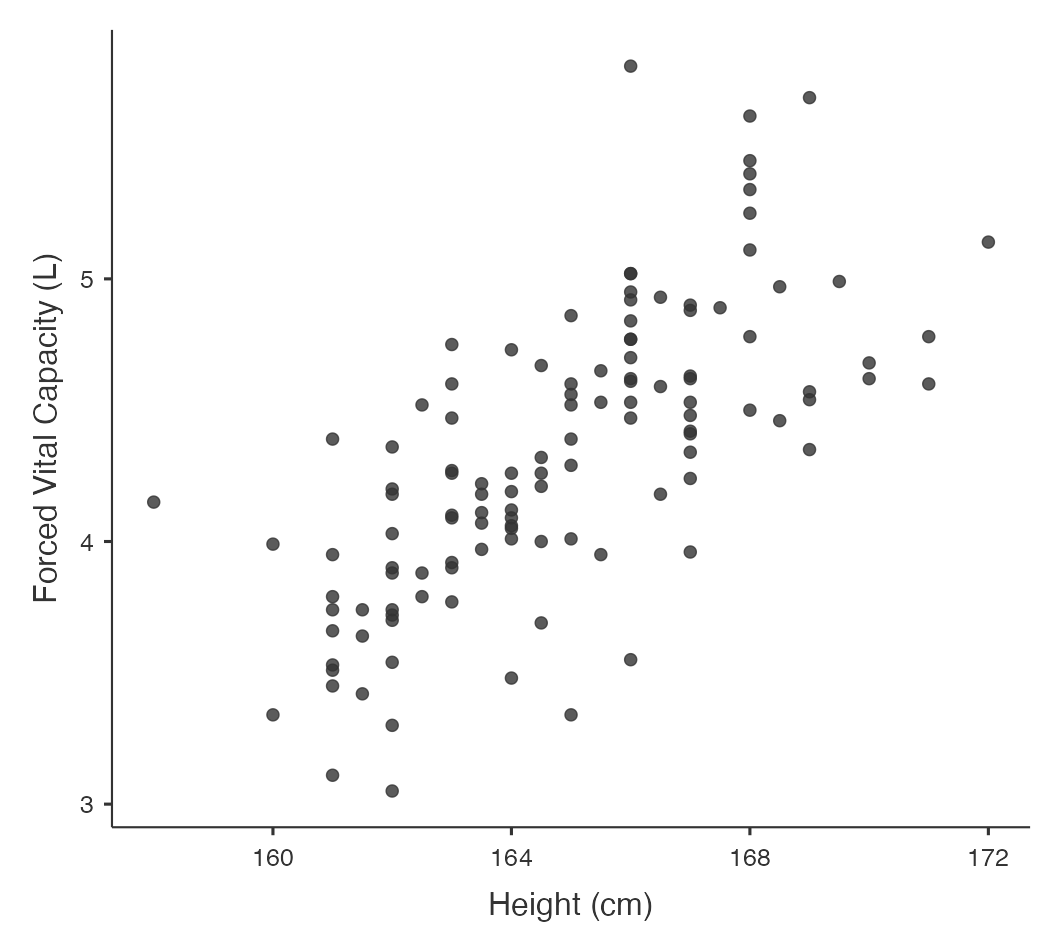
\includegraphics[width=0.5\linewidth,height=\textheight,keepaspectratio]{img/mod08/scatterpng.png}

}

\caption{\label{fig-scatter-plot}Association between height and lung
function in 120 adults}

\end{figure}%

\subsection{Correlation coefficients}\label{correlation-coefficients}

A correlation coefficient (r) describes how closely the variables are
related, that is the strength of linear association between two
continuous variables. The range of the coefficient is from +1 to −1
where +1 is a perfect positive association, 0 is no association and −1
is a perfect inverse association. One interpretation of the strength of
correlation coefficients has been provided by Schober et al. (2018)
(Table~\ref{tbl-r-strength}).

\begin{table}[h]

\caption{\label{tbl-r-strength}Interpretation of correlation
coefficients}

\centering{

\centering
\begin{tblr}[         %% tabularray outer open
]                     %% tabularray outer close
{                     %% tabularray inner open
colspec={Q[]Q[]},
hline{2}={1-2}{solid, black, 0.05em},
hline{1}={1-2}{solid, black, 0.08em},
hline{7}={1-2}{solid, black, 0.08em},
}                     %% tabularray inner close
Correlation coefficient (ignoring sign) & Strength of association \\
0 to <0.1 & Negligible \\
0.1 to <0.4 & Weak \\
0.4 to <0.7 & Moderate \\
0.7 to <0.9 & Strong \\
0.9 to 1.0 & Very strong \\
\end{tblr}

}

\end{table}%

The correlation coefficient is positive when large values of one
variable tend to occur with large values of the other, and small values
of one variable (y) tend to occur with small values of the other (x)
(Figure~\ref{fig-scatter-plot-four} (a and b)). For example, height and
weight in healthy children or age and blood pressure.

The correlation coefficient is negative when large values of one
variable tend to occur with small values of the other, and small values
of one variable tend to occur with large values of the other
(Figure~\ref{fig-scatter-plot-four} (c and d)). For example, percentage
immunised against infectious diseases and under-five mortality rate.

\begin{figure}

\centering{

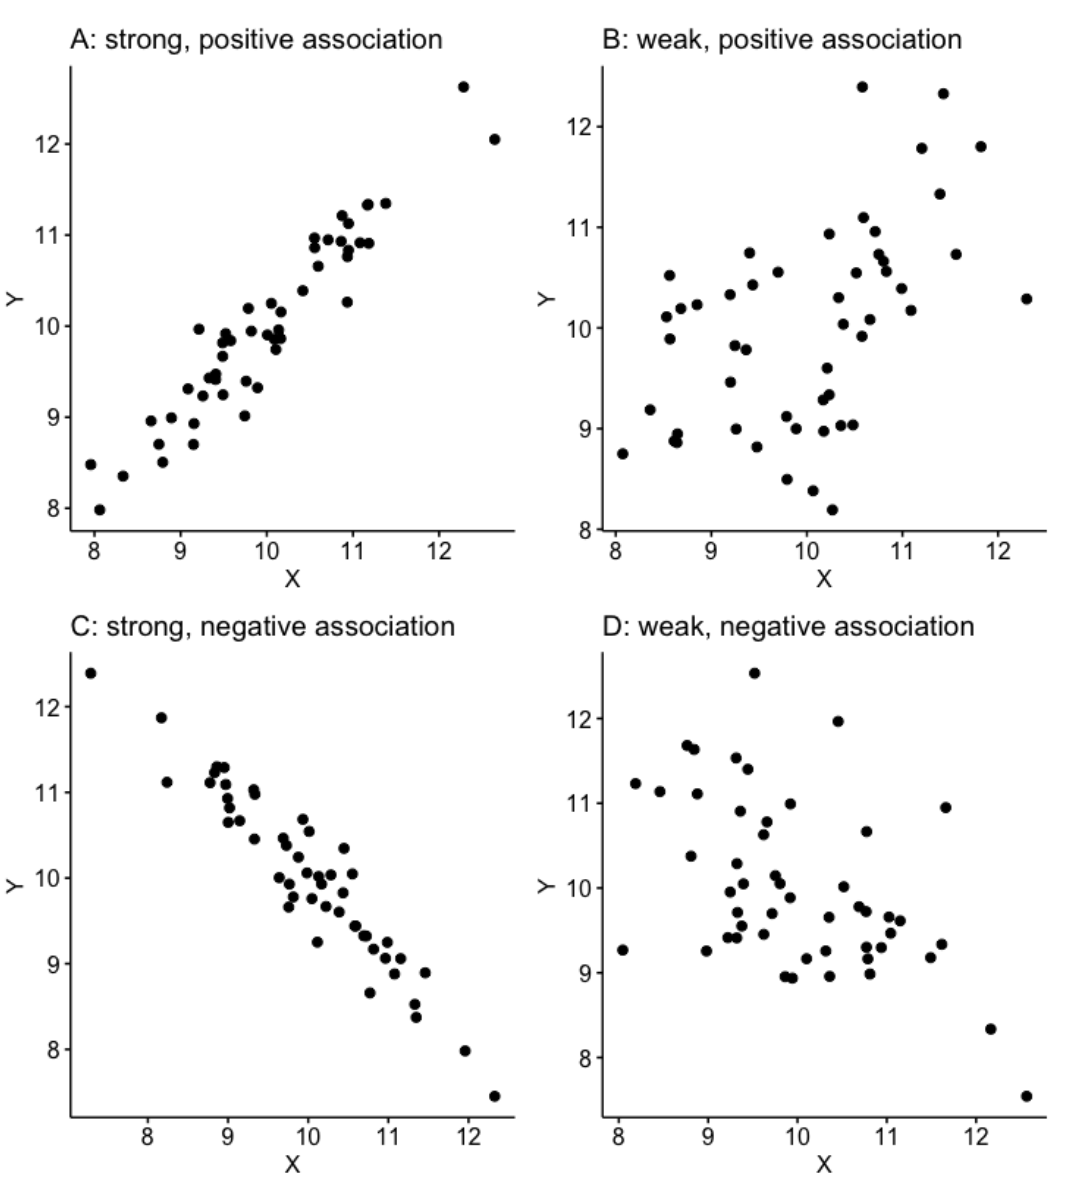
\includegraphics[width=0.66\linewidth,height=\textheight,keepaspectratio]{img/mod08/scatterplot-four-plots.png}

}

\caption{\label{fig-scatter-plot-four}Scatter plots demonstrating strong
and weak, positive and negative associations}

\end{figure}%

As with all estimates, a 95\% confidence interval should be provided
when providing a correlation coefficient. The calculation of the 95\%
confidence interval is beyond the scope of this course, but the interval
can be calculated easily by software.

It is also possible to calculate a P-value associated with a correlation
coefficient to test whether the correlation coefficient is different
from zero. However, a correlation coefficient with a large P-value does
not imply that there is no relationship between \(x\) and \(y\), because
the correlation coefficient only tests for a linear association and
there may be a non-linear relationship such as a curved or irregular
relationship.

The assumptions for using a Pearson's correlation coefficient are that:

\begin{itemize}
\tightlist
\item
  observations are independent;
\item
  both variables are continuous variables;
\item
  the relationship between the two variables is linear.
\end{itemize}

There is a further assumption that the data follow a bivariate normal
distribution. This assumes: \emph{y} follows a normal distribution for
given values of \emph{x}; and \emph{x} follows a normal distribution for
given values of \emph{y}. This is quite a technical assumption that we
do not discuss further.

There are two types of correlation coefficients, the correct one to use
is determined by the nature of the variables as shown in
Table~\ref{tbl-mod08-correlation-coefficients}.

\begin{longtable}[]{@{}
  >{\raggedright\arraybackslash}p{(\linewidth - 2\tabcolsep) * \real{0.2929}}
  >{\raggedright\arraybackslash}p{(\linewidth - 2\tabcolsep) * \real{0.7071}}@{}}
\caption{Correlation coefficients and their
application}\label{tbl-mod08-correlation-coefficients}\tabularnewline
\toprule\noalign{}
\begin{minipage}[b]{\linewidth}\raggedright
Correlation coefficient
\end{minipage} & \begin{minipage}[b]{\linewidth}\raggedright
Application
\end{minipage} \\
\midrule\noalign{}
\endfirsthead
\toprule\noalign{}
\begin{minipage}[b]{\linewidth}\raggedright
Correlation coefficient
\end{minipage} & \begin{minipage}[b]{\linewidth}\raggedright
Application
\end{minipage} \\
\midrule\noalign{}
\endhead
\bottomrule\noalign{}
\endlastfoot
Pearson's correlation coefficient: \(r\) & Both variables are continuous
and a bivariate normal distribution can be assumed \\
Spearman's rank correlation: \(\rho\) & Bivariate normality cannot be
assumed. Also useful when at least one of the variables is ordinal \\
\end{longtable}

Spearman's \(\rho\) is calculated using the ranks of the data, rather
than the actual values of the data. We will see further examples of such
methods in Module 9, when we consider non-parametric tests, which are
often based on ranks.

Correlation coefficients are often presented in the form of a
\emph{correlation matrix} which can display the correlation between a
number of variables in a single table (Table~\ref{tbl-corrmatrix}).

\begin{longtable}[]{@{}
  >{\raggedright\arraybackslash}p{(\linewidth - 4\tabcolsep) * \real{0.2125}}
  >{\raggedright\arraybackslash}p{(\linewidth - 4\tabcolsep) * \real{0.3875}}
  >{\raggedright\arraybackslash}p{(\linewidth - 4\tabcolsep) * \real{0.3875}}@{}}
\caption{Correlation matrix for Height and
FVC}\label{tbl-corrmatrix}\tabularnewline
\toprule\noalign{}
\begin{minipage}[b]{\linewidth}\raggedright
\end{minipage} & \begin{minipage}[b]{\linewidth}\raggedright
Height
\end{minipage} & \begin{minipage}[b]{\linewidth}\raggedright
FVC
\end{minipage} \\
\midrule\noalign{}
\endfirsthead
\toprule\noalign{}
\begin{minipage}[b]{\linewidth}\raggedright
\end{minipage} & \begin{minipage}[b]{\linewidth}\raggedright
Height
\end{minipage} & \begin{minipage}[b]{\linewidth}\raggedright
FVC
\end{minipage} \\
\midrule\noalign{}
\endhead
\bottomrule\noalign{}
\endlastfoot
Height & 1 & \begin{minipage}[t]{\linewidth}\raggedright
0.70 (95\% CI: 0.59 to 0.78)\\
P \textless{} 0.0001\strut
\end{minipage} \\
FVC & \begin{minipage}[t]{\linewidth}\raggedright
0.70 (95\% CI: 0.59 to 0.78)\\
P \textless{} 0.0001\strut
\end{minipage} & 1 \\
\end{longtable}

This correlation matrix shows that there is a strong association between
height and lung function (r = 0.70, 95\% CI: 0.59 to 0.78). The P-value
(\textless0.0001) indicates there is very strong evidence of a linear
association between height and FVC.

A correlation matrix sometimes includes correlations between the same
variable, indicated as a correlation coefficient of 1. For example,
\(Height\) is perfectly correlated with itself (i.e.~has a correlation
coefficient of 1). Similarly, \(FVC\) is perfectly correlated with
itself.

Correlation coefficients are rarely used as important statistics in
their own right because they do not fully explain the relationship
between the two variables and the range of the data has an important
influence on the size of the coefficient. In addition, the statistical
significance of the correlation coefficient is often over interpreted
because a small correlation which is of no clinical importance can
become statistically significant even with a relatively small sample
size. For example, a weak correlation of 0.3 will be statistically
significant if the sample size is large enough.

\section{Linear regression}\label{linear-regression}

The nature of a relationship between two variables is more fully
described using regression, where the relationship is described by a
straight line.

Figure~\ref{fig-scatter-plot-line} shows our lung data with a fitted
regression line.

\begin{figure}

\centering{

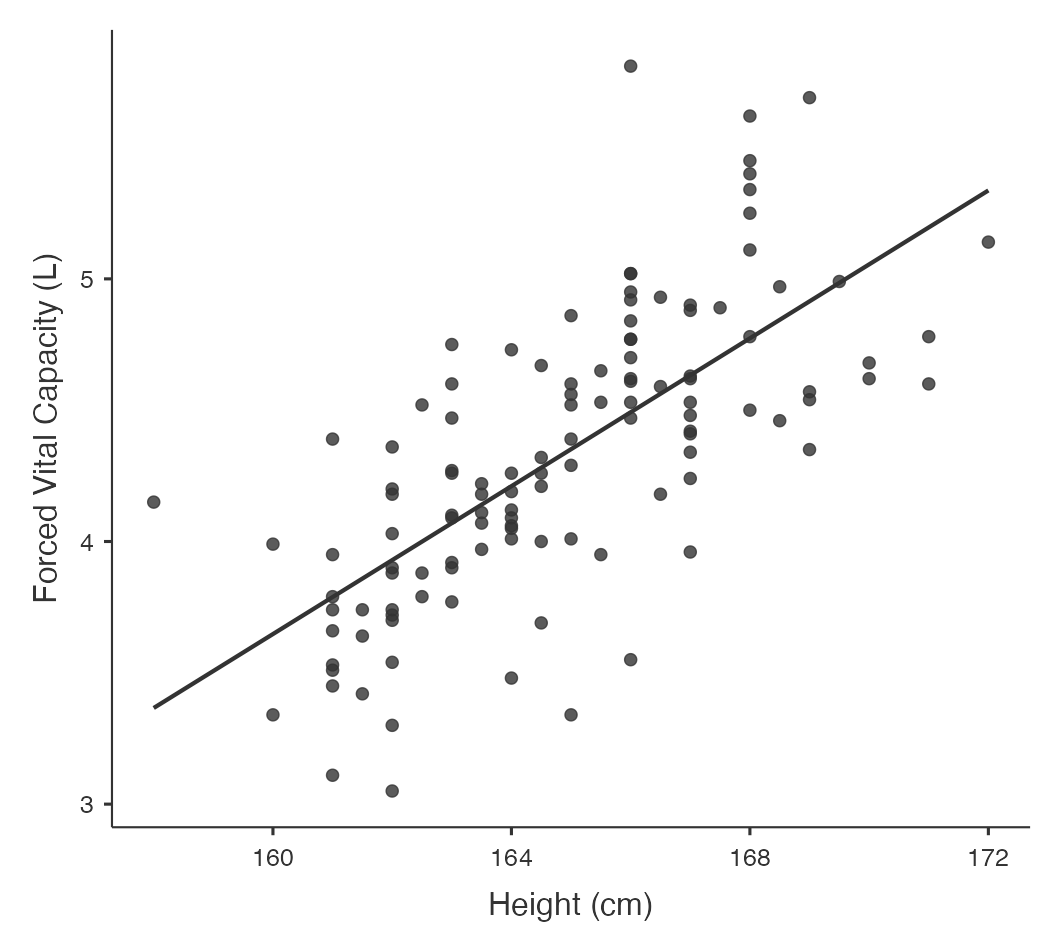
\includegraphics[width=0.66\linewidth,height=\textheight,keepaspectratio]{img/mod08/scatterplot-line-fvc-height.png}

}

\caption{\label{fig-scatter-plot-line}Association between height and
lung function in 120 adults}

\end{figure}%

The line through the plot is called the line of `best fit' because the
size of the deviations between the data points and the line is minimised
in estimating the line.

\subsection{Regression equations}\label{regression-equations}

The mathematical equation for the line explains the relationship between
two variables: \(y\), the outcome variable, and \(x\), the explanatory
variable. The equation of the regression line is as follows:

\[y = \beta_{0} + \beta_{1}x\]

This line is shown in Figure~\ref{fig-regression-parameters} using the
notation shown in Table~\ref{tbl-regression-notation}.

\begin{figure}

\centering{

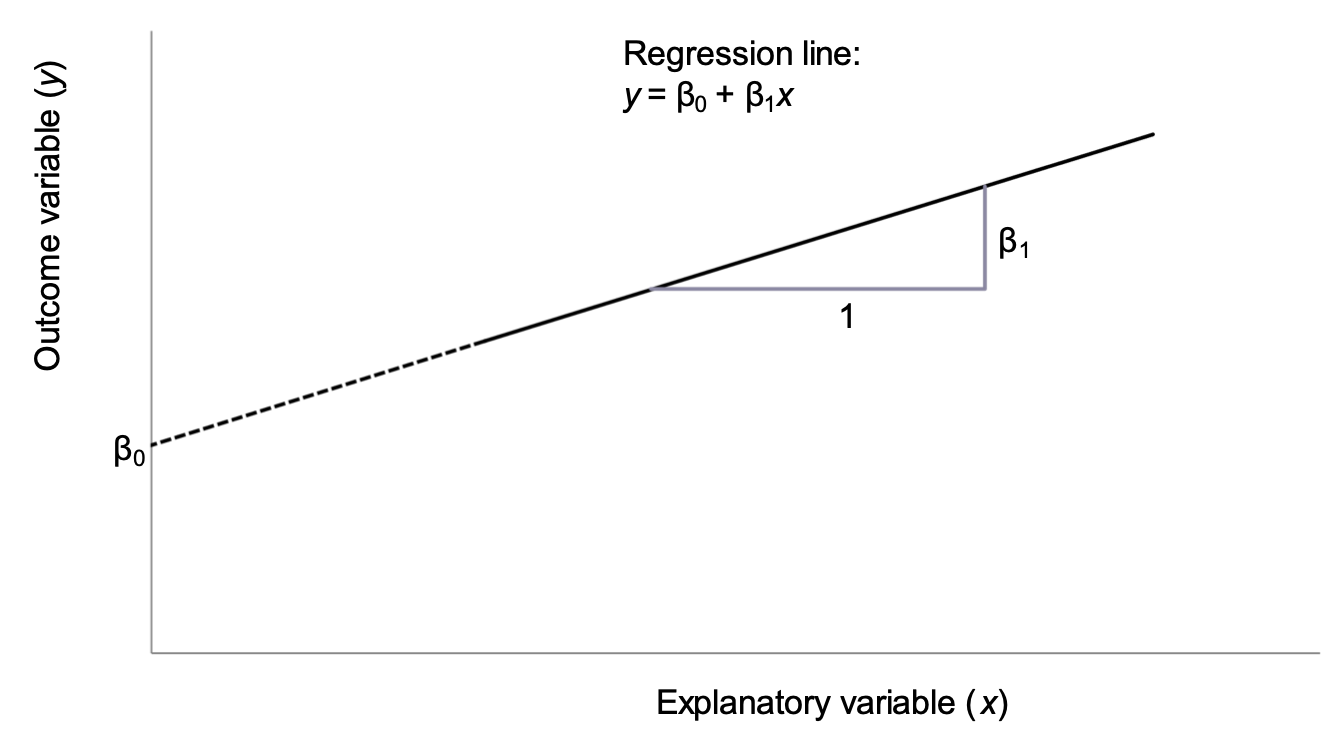
\includegraphics[width=0.66\linewidth,height=\textheight,keepaspectratio]{img/mod08/regression-line-parameters.png}

}

\caption{\label{fig-regression-parameters}Coefficients of a linear
regression equation}

\end{figure}%

\begin{longtable}[]{@{}
  >{\raggedright\arraybackslash}p{(\linewidth - 2\tabcolsep) * \real{0.2639}}
  >{\raggedright\arraybackslash}p{(\linewidth - 2\tabcolsep) * \real{0.6667}}@{}}
\caption{Notation for linear regression
equation}\label{tbl-regression-notation}\tabularnewline
\toprule\noalign{}
\begin{minipage}[b]{\linewidth}\raggedright
Symbol
\end{minipage} & \begin{minipage}[b]{\linewidth}\raggedright
Interpretation
\end{minipage} \\
\midrule\noalign{}
\endfirsthead
\toprule\noalign{}
\begin{minipage}[b]{\linewidth}\raggedright
Symbol
\end{minipage} & \begin{minipage}[b]{\linewidth}\raggedright
Interpretation
\end{minipage} \\
\midrule\noalign{}
\endhead
\bottomrule\noalign{}
\endlastfoot
\(y\) & The outcome variable \\
\(x\) & The explanatory variable \\
\(\beta_0\) & Intercept of the regression line \\
\(\beta_1\) & Slope of the regression line \\
\end{longtable}

The intercept is the point at which the regression line intersects with
the y-axis when the value of \(x\) is zero. In most cases, the intercept
does not have a biologically meaningful interpretation as the
explanatory variable cannot take a value of zero. In our working
example, the intercept is not meaningful as it is not possible for an
adult to have a height of 0cm.

The slope of the line is the predicted change in the outcome variable
\(y\) as the explanatory explanatory variable \(x\) increases by 1 unit.

An important concept is that regression predicts an expected value of
\(y\) given an observed value of \(x\): any error around the explanatory
variable is not taken into account.

\section{Regression coefficients:
estimation}\label{regression-coefficients-estimation}

The regression parameters \(\beta_{0}\) and \(\beta_{1}\) are true,
unknown quantities (similar to \(\mu\) and \(\sigma\)), which are
estimated using statistical software using the \emph{method of least
squares}. This method estimates the intercept and the slope, and also
their variability (i.e.~standard errors). Software is always used to
estimate the regression parameters from a set of data.

Using the method of least squares:

\begin{itemize}
\tightlist
\item
  the intercept is estimated as \(b_0\);
\item
  the slope is estimated as \(b_1\).
\end{itemize}

\section{Regression coefficients:
inference}\label{regression-coefficients-inference}

We can use the estimated regression coefficients and their variability
to calculate 95\% confidence intervals. Here, a t-value from a
t-distribution with \(n - 2\) degrees of freedom is used:

\begin{itemize}
\tightlist
\item
  95\% confidence interval for intercept:
  \(b_0 \pm t_{n-2} \times SE(b_0)\)
\item
  95\% confidence interval for slope: \(b_1 \pm t_{n-2} \times SE(b_1)\)
\end{itemize}

Note that as the constant (\(b_0\)) is not often biologically plausible,
the 95\% confidence interval for the constant is often not reported.

The significance of the estimated slope (and less commonly, intercept)
can be tested using a t-test. The null hypotheses and the alternative
hypothesis for testing the slope of a simple linear regression model
are:

\begin{itemize}
\tightlist
\item
  H\textsubscript{0}: \(\beta_1 = 0\)
\item
  H\textsubscript{1}: \(\beta_1 \ne 0\)
\end{itemize}

To test the null hypothesis for the regression coefficient \(\beta_1\),
the following t-test is used:

\[t = b_1 /SE(b_1)\]

This will give a t statistic which can be referred to a t distribution
with n − 2 degrees of freedom to calculate the corresponding P-value.

Table~\ref{tbl-estimated-regression} shows the estimated regression
coefficients for our working example.

\begin{table}[h]

\caption{\label{tbl-estimated-regression}Estimated regression
coefficients}

\centering{

\centering
\begin{tblr}[         %% tabularray outer open
]                     %% tabularray outer close
{                     %% tabularray inner open
width={1\linewidth},
colspec={X[0.12]X[0.12]X[0.11]X[0.23]X[0.11]X[0.31]},
hline{2}={1-6}{solid, black, 0.05em},
hline{1}={1-6}{solid, black, 0.08em},
hline{4}={1-6}{solid, black, 0.08em},
column{4-6}={}{halign=c},
column{1-3}={}{halign=l},
}                     %% tabularray inner close
Term & Estimate & Standard error & t value & P value & 95\% Confidence interval \\
Intercept & -18.87 & 2.194 & t=-8.60, 118df & <0.001 & -23.22 to -14.53 \\
Height & 0.14 & 0.013 & t=10.58, 118df & <0.001 & 0.11 to 0.17 \\
\end{tblr}

}

\end{table}%

From this output, we see that the slope is estimated as 0.14 with an
estimated intercept of -18.87. Therefore, the regression equation is
estimated as:

FVC (L) = − 18.87 + (0.14 \(\times\) Height in cm)

There is very strong evidence of a linear association between FVC and
height in cm (P \textless{} 0.001).

This equation can be used to predict FVC for a person of a given height.
For example, the predicted FVC for a person 165 cm tall is estimated as:

FVC = − 18.87347 + (0.1407567 \(\times\) 165.0) = 4.40 L.

Note that for the purpose of prediction we have kept all the decimal
places in the coefficients to avoid rounding error in the intermediate
calculation.

\subsection{Fit of a linear regression
model}\label{fit-of-a-linear-regression-model}

After fitting a linear regression model, it is important to know how
well the model fits the observed data. One way of assessing the model
fit is to compute a statistic called coefficient of determination,
denoted by \(R^2\). It is the square of the Pearson correlation
coefficient \(r: r^2 = R^2\). Since the range of \(r\) is from −1 to 1,
\(R^2\) must lie between 0 and 1.

\(R^2\) can be interpreted as the proportion of variability in y that
can be explained by variability in x. Hence, the following conditions
may arise:

If \(R^2 = 1\), then all variation in y can be explained by variation of
x and all data points fall on the regression line.

If \(R^2 = 0\), then none of the variation in y is related to x at all,
and the variable x explains none of the variability in y.

If \(0 < R^2 <1\), then the variability of y can be partially explained
by the variability in x. The larger the \(R^2\) value, the better is the
fit of the regression model.

\section{Assumptions for linear
regression}\label{assumptions-for-linear-regression}

Regression is robust to moderate degrees of non-normality in the
variables, provided that the sample size is large enough and that there
are no influential outliers. Also, the regression equation describes the
relationship between the variables and this is not influenced as much by
the spread of the data as the correlation coefficient is.

The assumptions that must be met when using linear regression are as
follows:

\begin{itemize}
\tightlist
\item
  observations are independent;
\item
  the relationship between the explanatory and the outcome variable is
  linear;
\item
  the residuals are normally distributed.
\end{itemize}

A residual is defined as the difference between the observed and
predicted outcome from the regression model. If the predicted value of
the outcome variable is denoted by \(\hat y\) then:

\[ \text{Residual} = \text{observed} - \text{predicted} = y - \hat y\]

It is important for regression modelling that the data are collected in
a period when the relationship remains constant. For example, in
building a model to predict normal values for lung function the data
must be collected when the participants have been resting and not
exercising and people taking bronchodilator medications that influence
lung capacity should be excluded. In regression, it is not so important
that the variables themselves are normally distributed, but it is
important that the residuals are. Scatter plots and specific diagnostic
tests can be used to check the regression assumptions. Some of these
will not be covered in this introductory course but will be discussed in
detail in the \textbf{Regression Methods in Biostatistics} course.

The distribution of the residuals should always be checked. Large
residuals can indicate unusual points or points that may exert undue
influence on the estimated regression slope.

The distribution of the residuals from the model is shown in
Figure~\ref{fig-residual-dist}. The residuals are approximately normally
distributed, with no outlying values.

\begin{figure}

\centering{

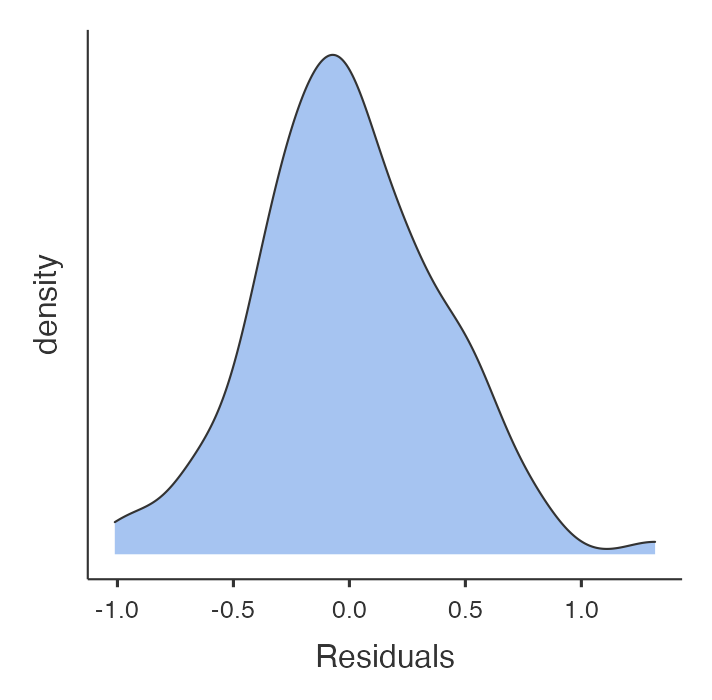
\includegraphics[width=0.5\linewidth,height=\textheight,keepaspectratio]{img/mod08/regression-residual-dist.png}

}

\caption{\label{fig-residual-dist}Distribution of regression residuals}

\end{figure}%

\section{Multiple linear regression}\label{multiple-linear-regression}

In the above example, we have only used a simple linear regression model
of two continuous variables. Other more complex models can be built from
this e.g.~if we wanted to look at the effect of gender (male vs.~female)
as binary indicator in the model while adjusting for the effect of
height. In that case we would include both the variables in the model as
explanatory variables. In the same way we can include any number of
explanatory variables (both continuous and categorical) in the model:
this is called a multivariable model. Multivariable models are often
used for building predictive equations, for example by using age,
height, gender and smoking history to predict lung function, or to
adjust for confounding and detect effect modification to investigate the
association between an exposure and an outcome factor.

Multiple regression has an important role in investigating causality in
epidemiology. The exposure variable under investigation must stay in the
model and the effects of other variables which can be confounders or
effect-modifiers are tested. The biological, psychological or social
meaning of the variables in the model and their interactions are of
great importance for interpreting theories of causality.

Other multivariable models include binary logistic regression for use
with a binary outcome variable, or Cox regression for survival analyses.
These models, together with multiple regression, will be taught in
\textbf{PHCM9517: Regression Methods in Biostatistics}.

\newpage{}

\bookmarksetup{startatroot}

\chapter*{Jamovi notes}\label{jamovi-notes-6}
\addcontentsline{toc}{chapter}{Jamovi notes}

\markboth{Jamovi notes}{Jamovi notes}

\section{Creating a scatter plot}\label{creating-a-scatter-plot}

We will demonstrate using Jamovi for correlation and simple linear
regression using the dataset \texttt{mod08\_lung\_function.csv}.

To create a scatter plot to explore the association between height and
FVC, we use \textbf{Scatterplot} within the \textbf{Exploration} menu:

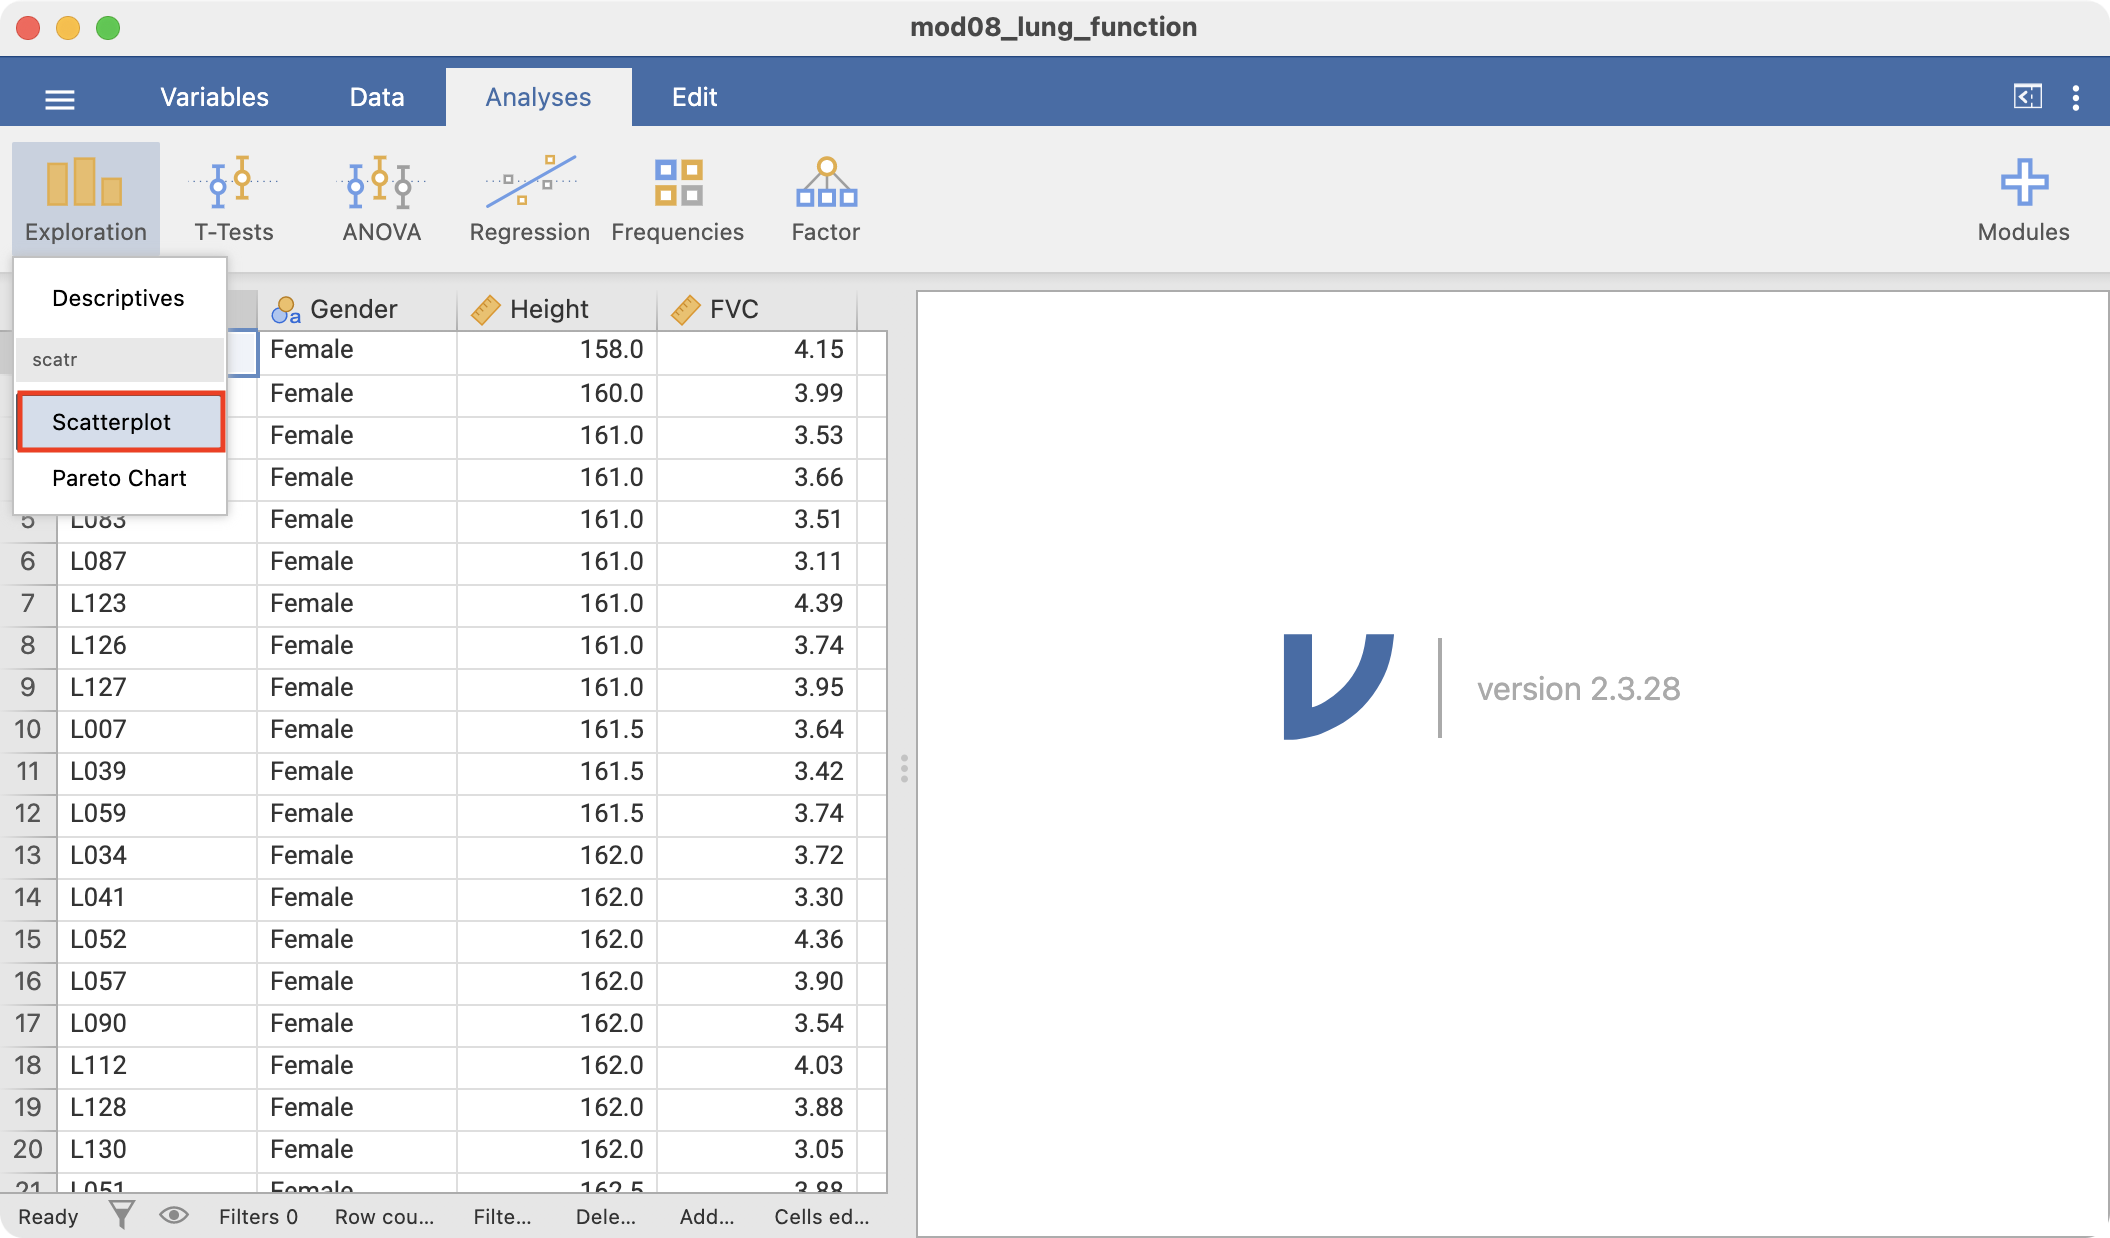
\includegraphics[width=0.8\linewidth,height=\textheight,keepaspectratio]{img/mod08/jamovi/twoway-1.png}

Choose \textbf{Height} for the \textbf{X-Axis}, and \textbf{FVC} for the
\textbf{Y-Axis}, and the scatter-plot appears in the Output window:

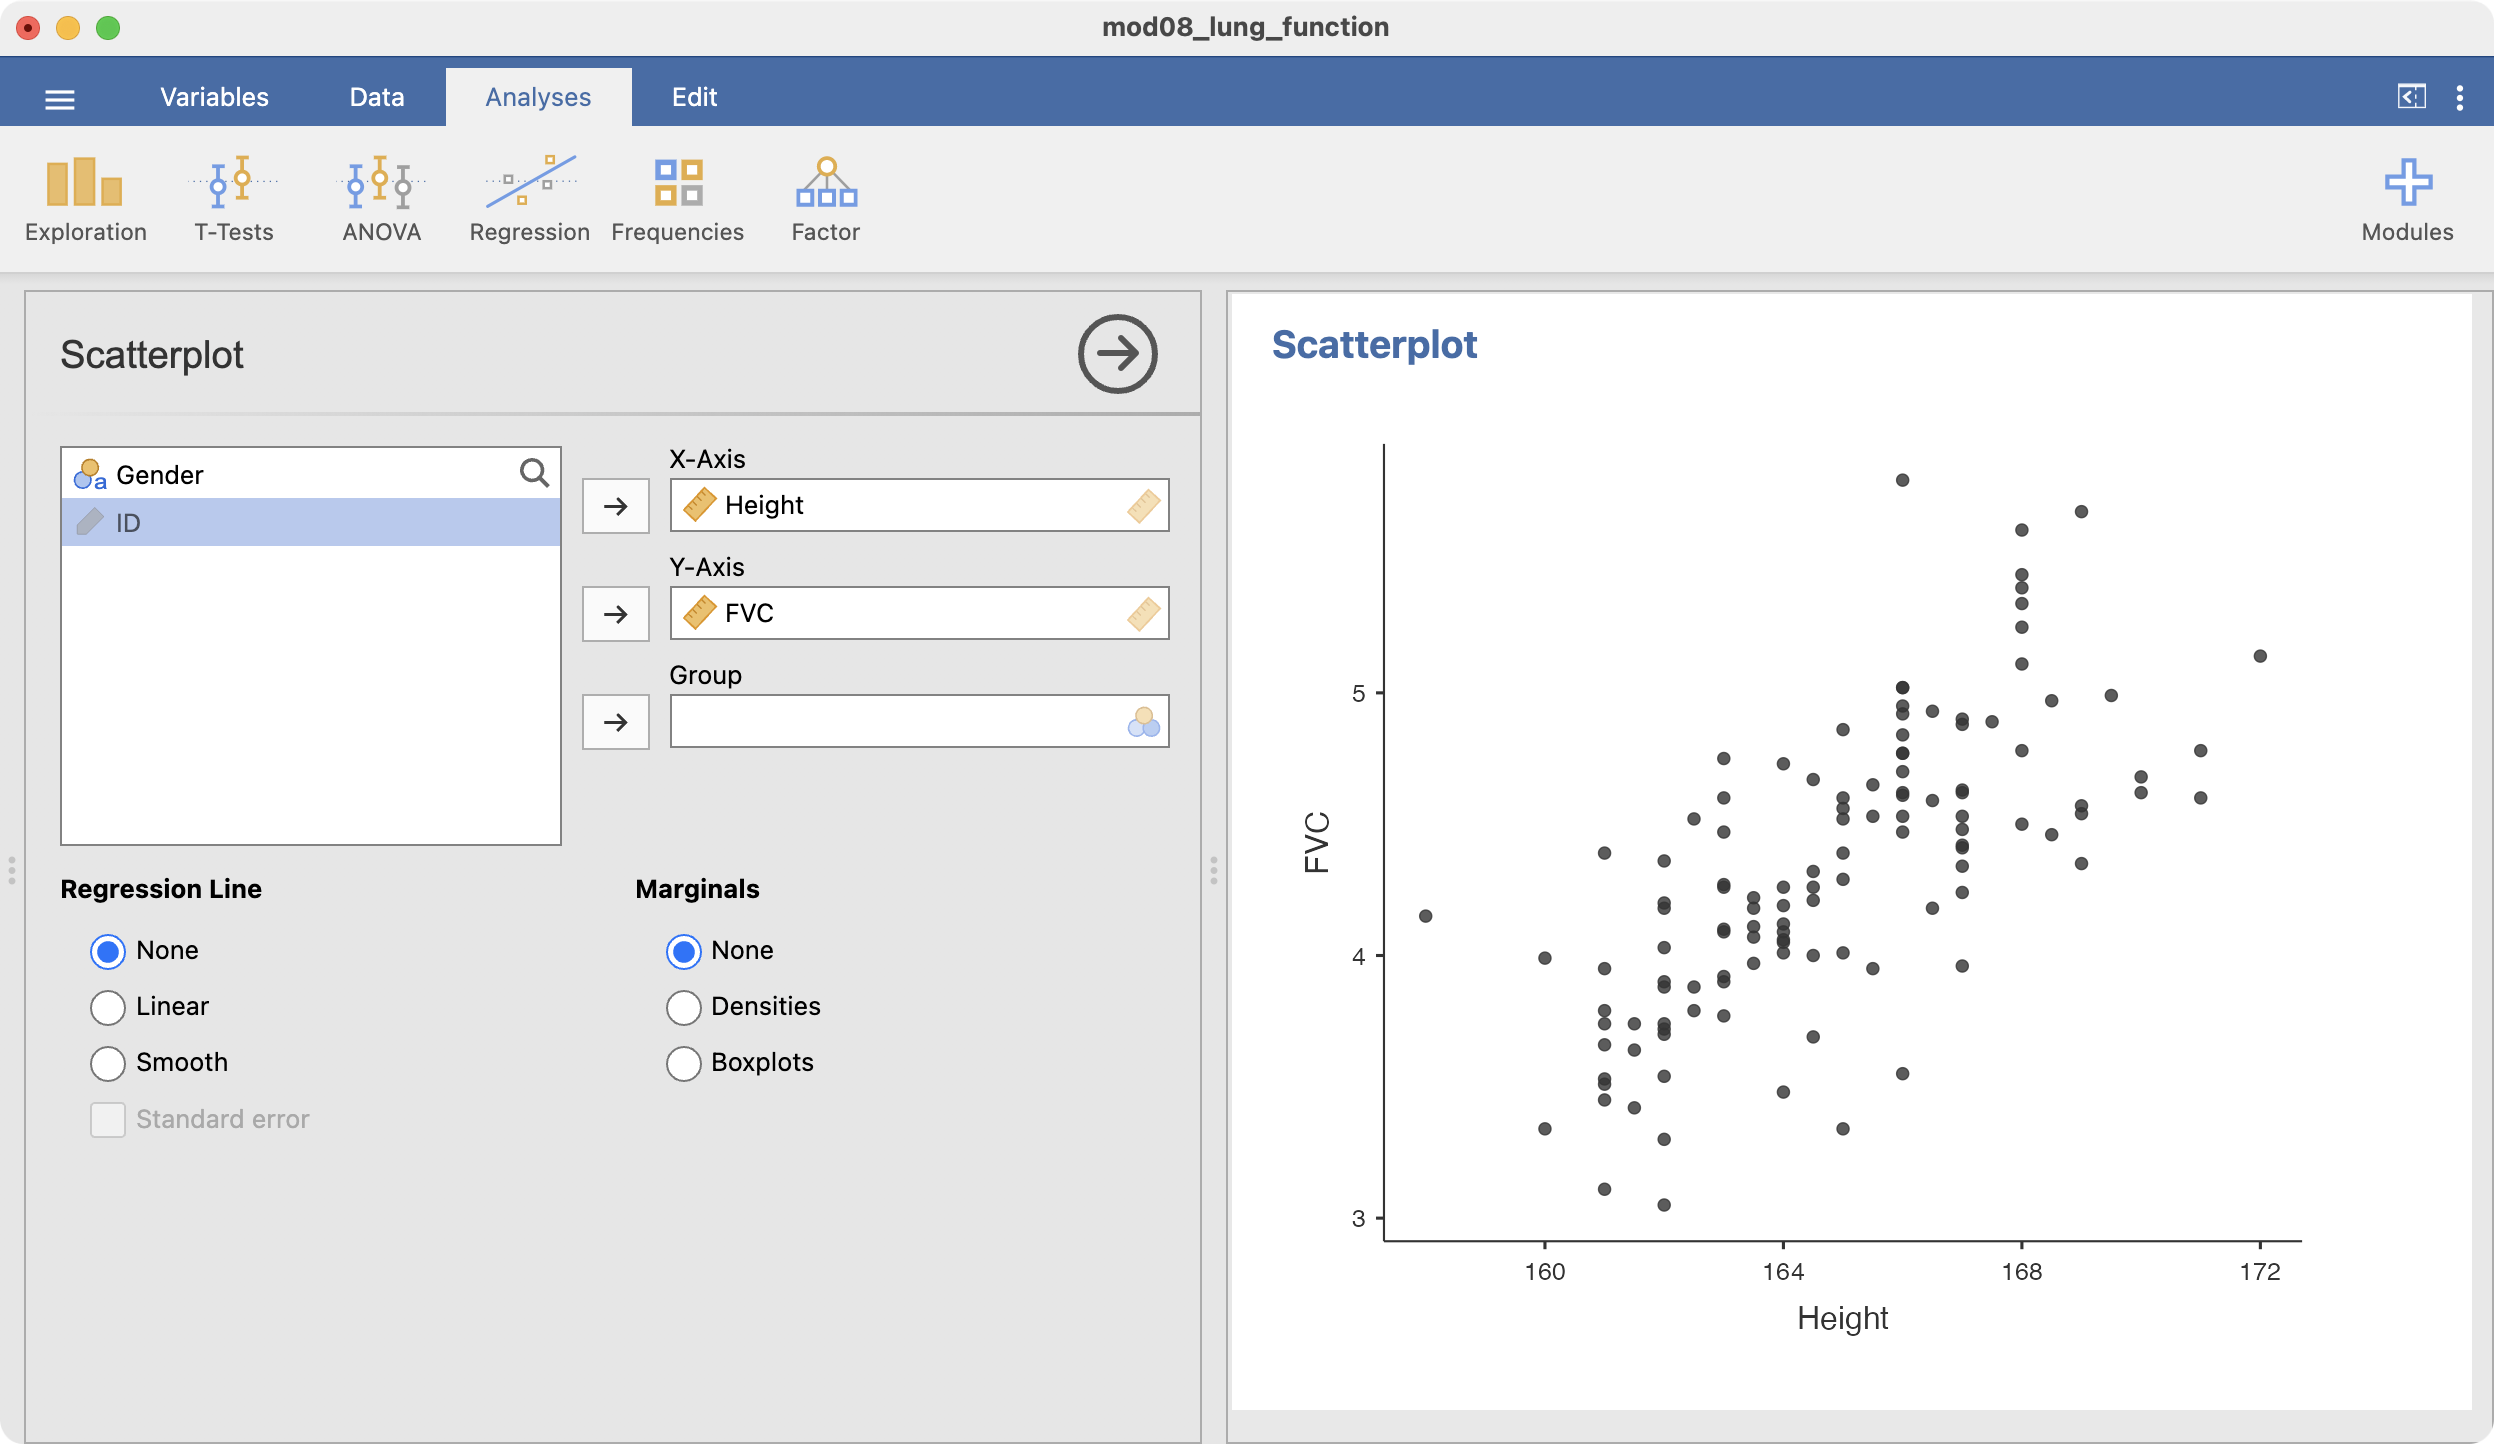
\includegraphics[width=0.8\linewidth,height=\textheight,keepaspectratio]{img/mod08/jamovi/twoway-2.png}

To add a fitted line, click the \textbf{Linear} option in the
\textbf{Regression Line} section:

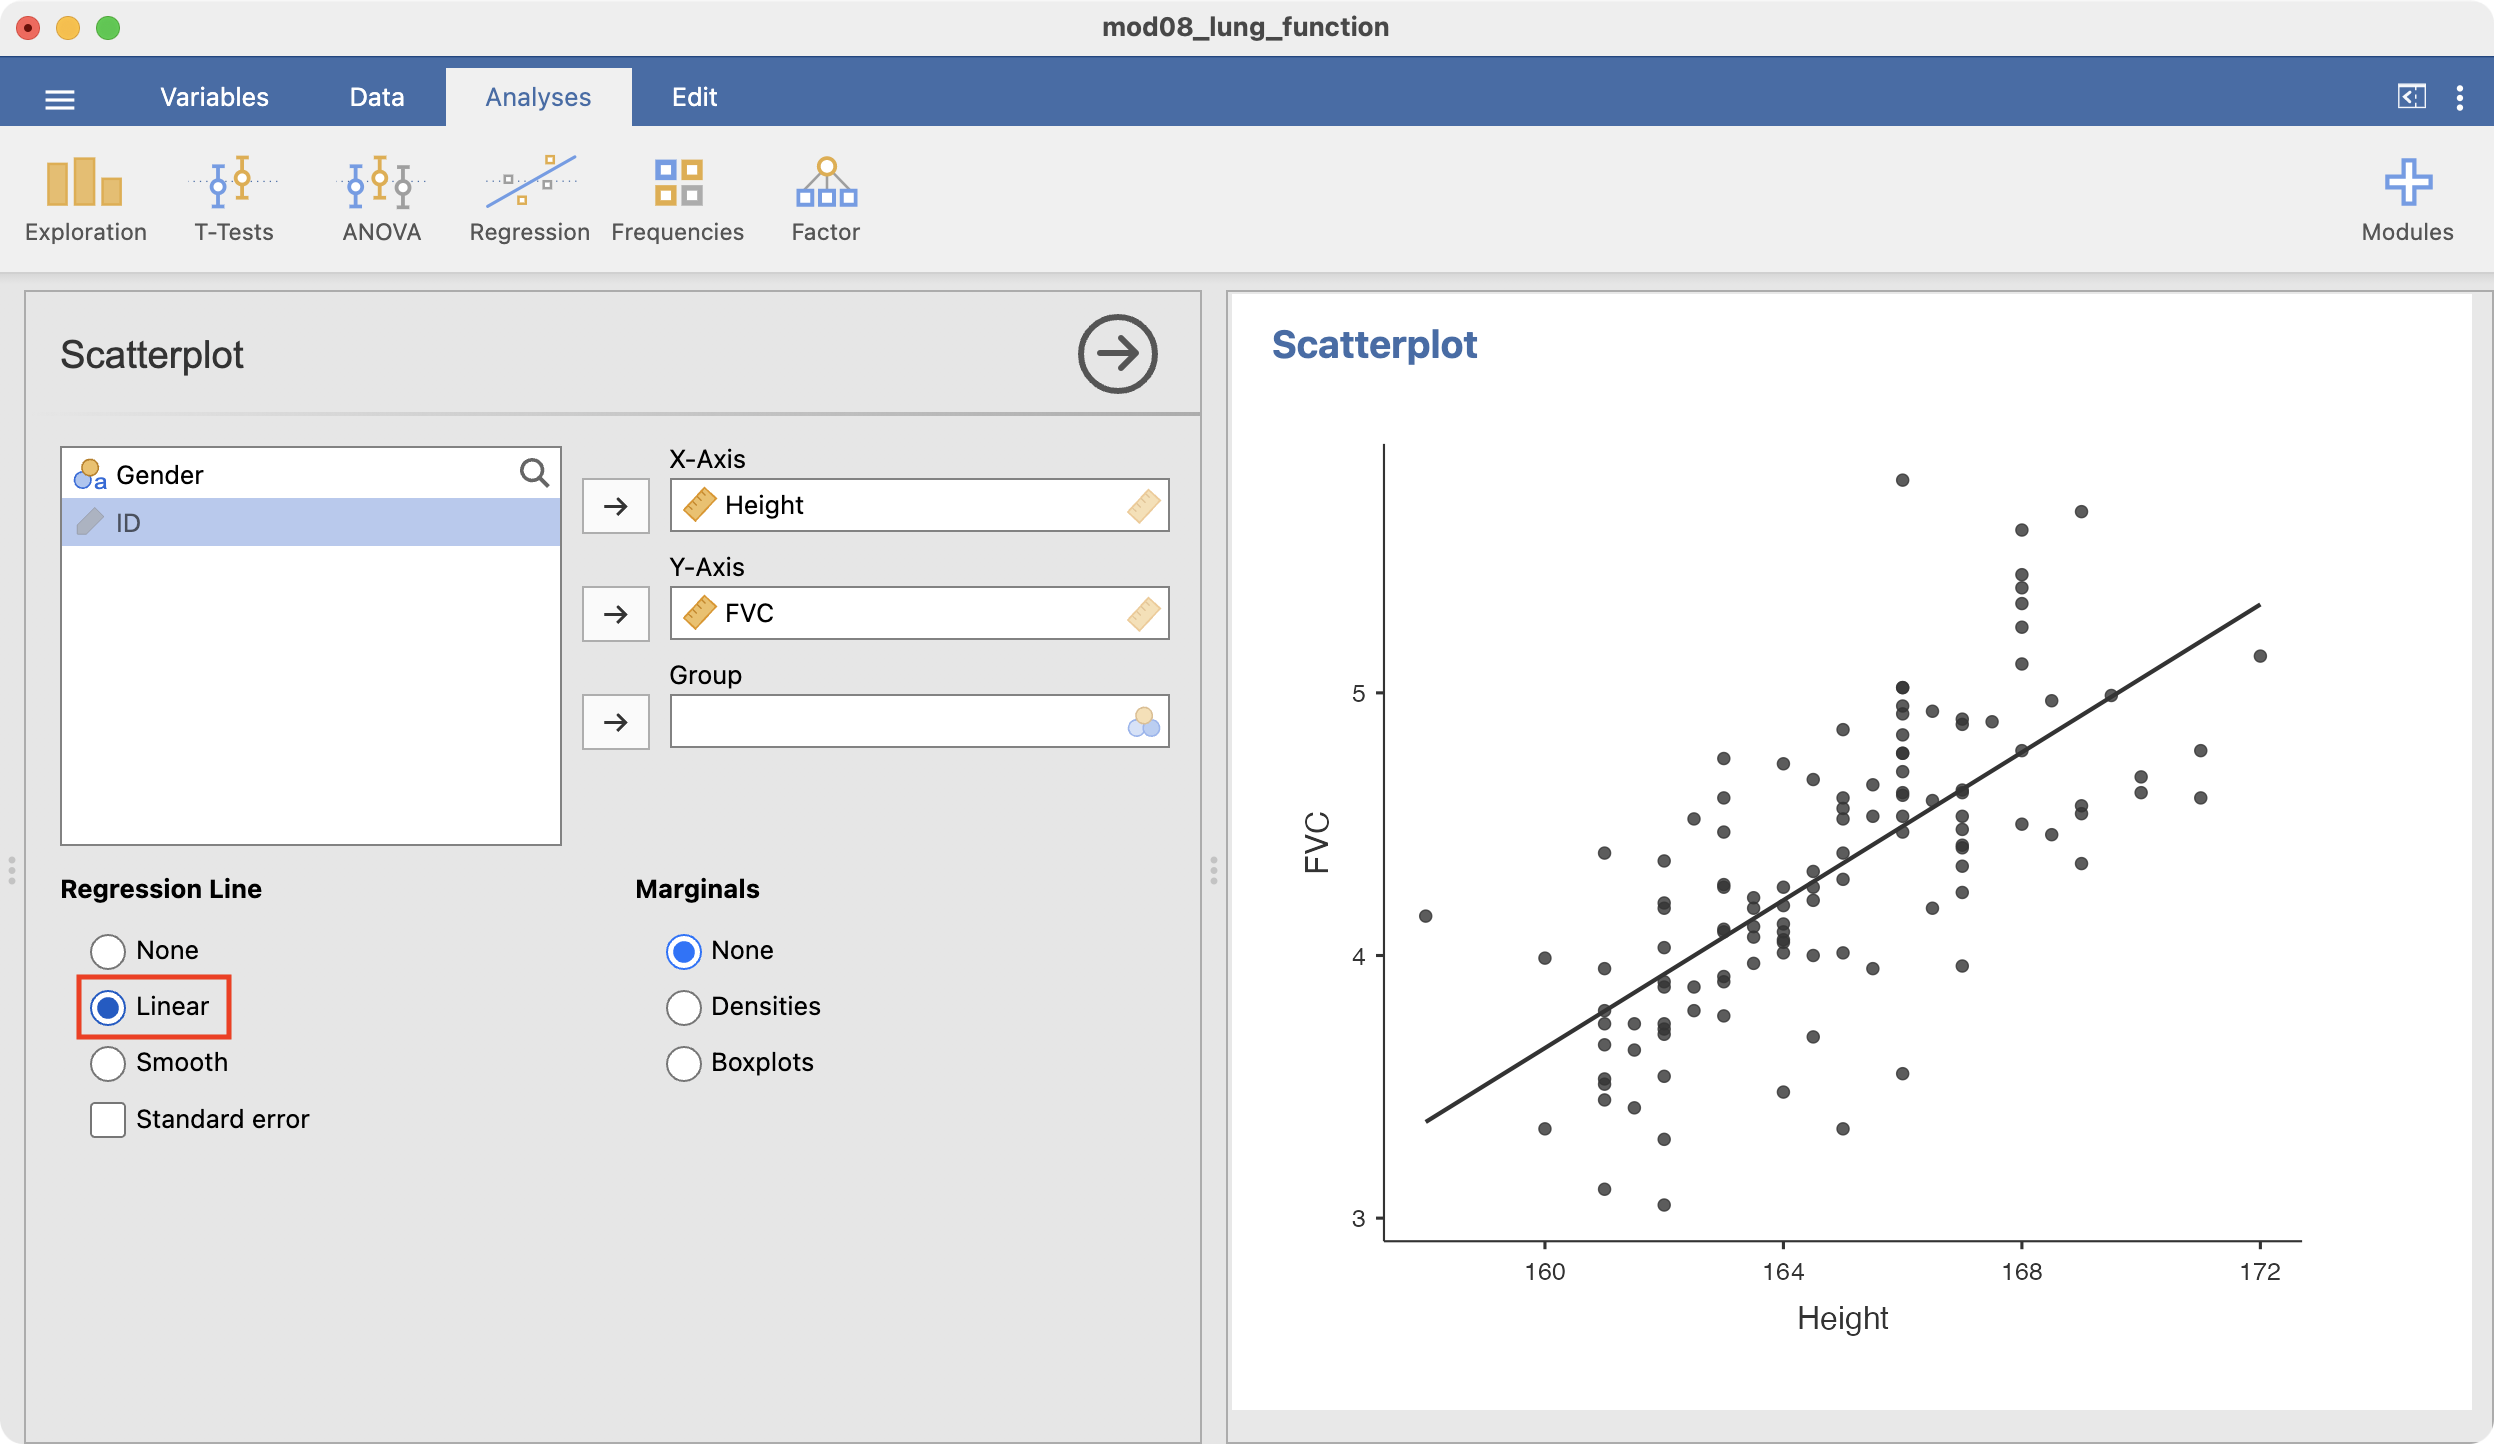
\includegraphics[width=0.8\linewidth,height=\textheight,keepaspectratio]{img/mod08/jamovi/twoway-3.png}

To save your graph, right-click the graph and choose \textbf{Image
\textgreater{} Export}, and be sure to save your file as a PNG file:

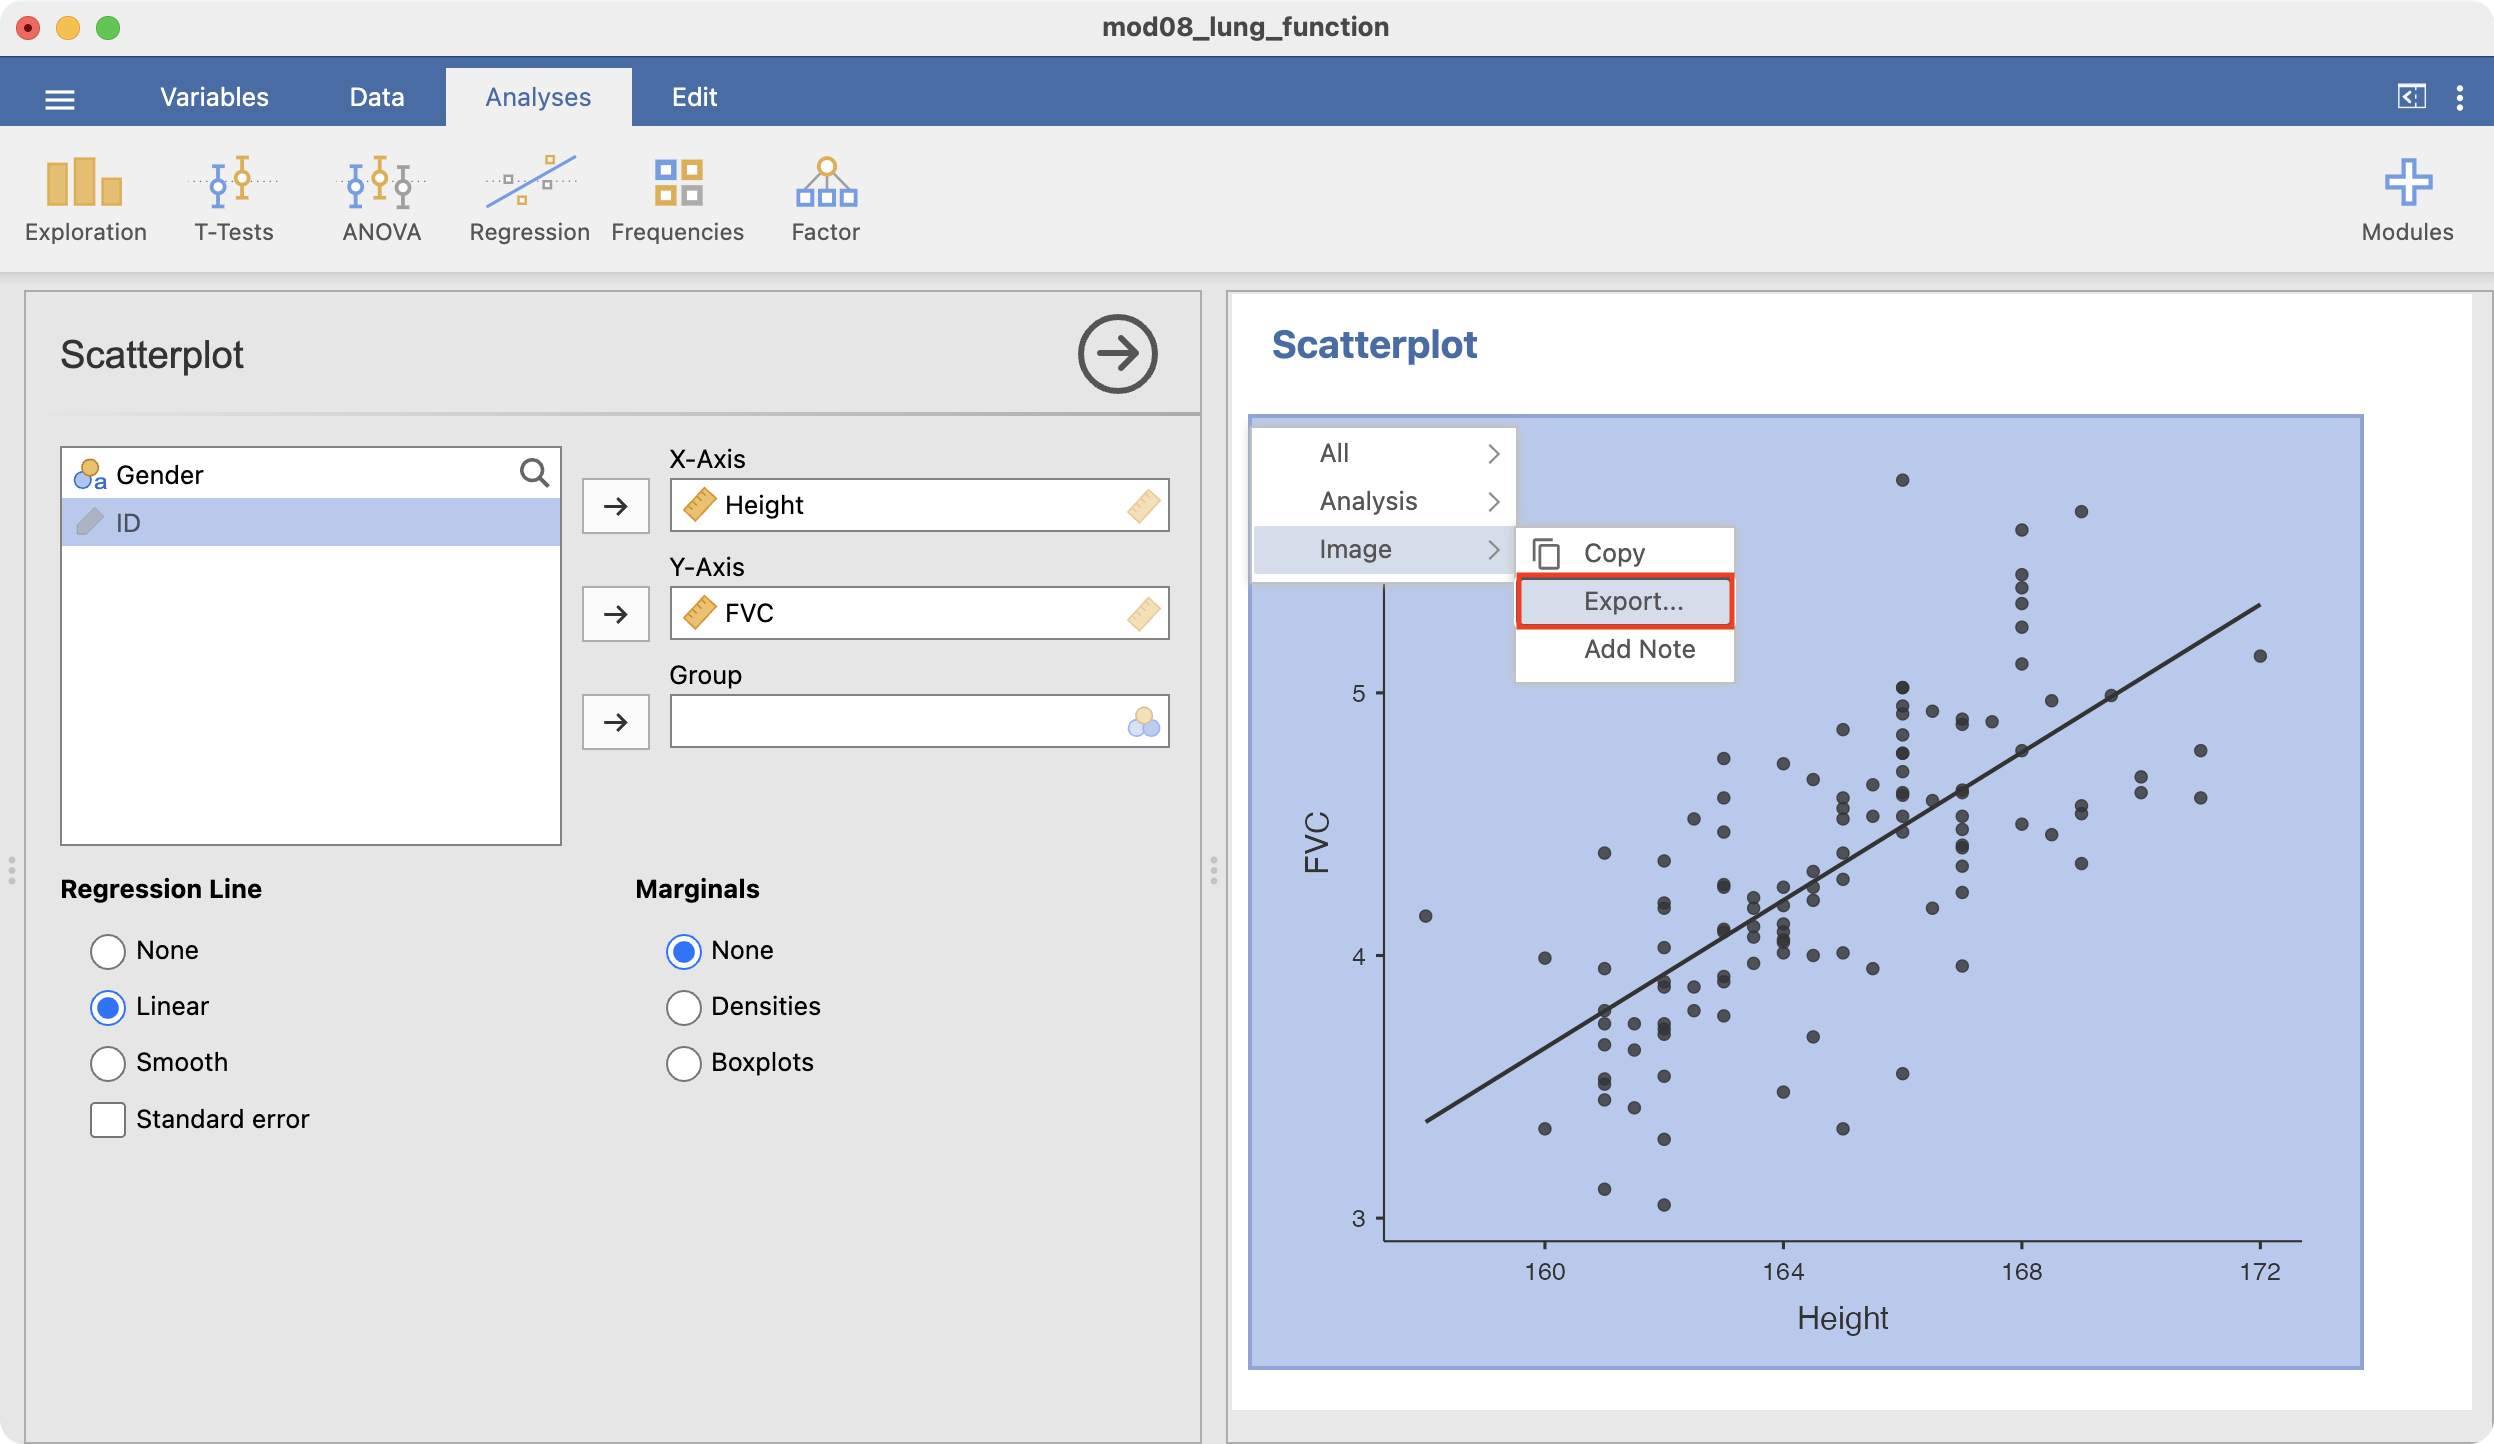
\includegraphics[width=0.8\linewidth,height=\textheight,keepaspectratio]{img/mod08/jamovi/twoway-7.png}

\section{Calculating a correlation
coefficient}\label{calculating-a-correlation-coefficient}

To calculate the Pearson's correlation using the dataset
\texttt{mod08\_lung\_function.csv} choose: \textbf{Correlation Matrix}
within the \textbf{Regression} menu.

Select the two variables, \textbf{FVC} and \textbf{Height} in the
\textbf{Variables} box, and tick \textbf{Confidence intervals}. A
correlation matrix will be constructed, similar to
Table~\ref{tbl-corrmatrix}.

\section{Fitting a simple linear regression
model}\label{fitting-a-simple-linear-regression-model}

To fit a simple linear regression model, choose \textbf{Regression
\textgreater{} Linear Regression}

Select \texttt{FVC} as the \textbf{Dependent variable}, and
\texttt{Height} as a \textbf{Covariate} (Jamovi refers to continuous
explanatory variables as \emph{covariates}). To obtain the 95\%
confidence interval for the regression coefficients, scroll down to the
\textbf{Model Coefficients} section and click the \textbf{Confidence
interval} option for Estimate.

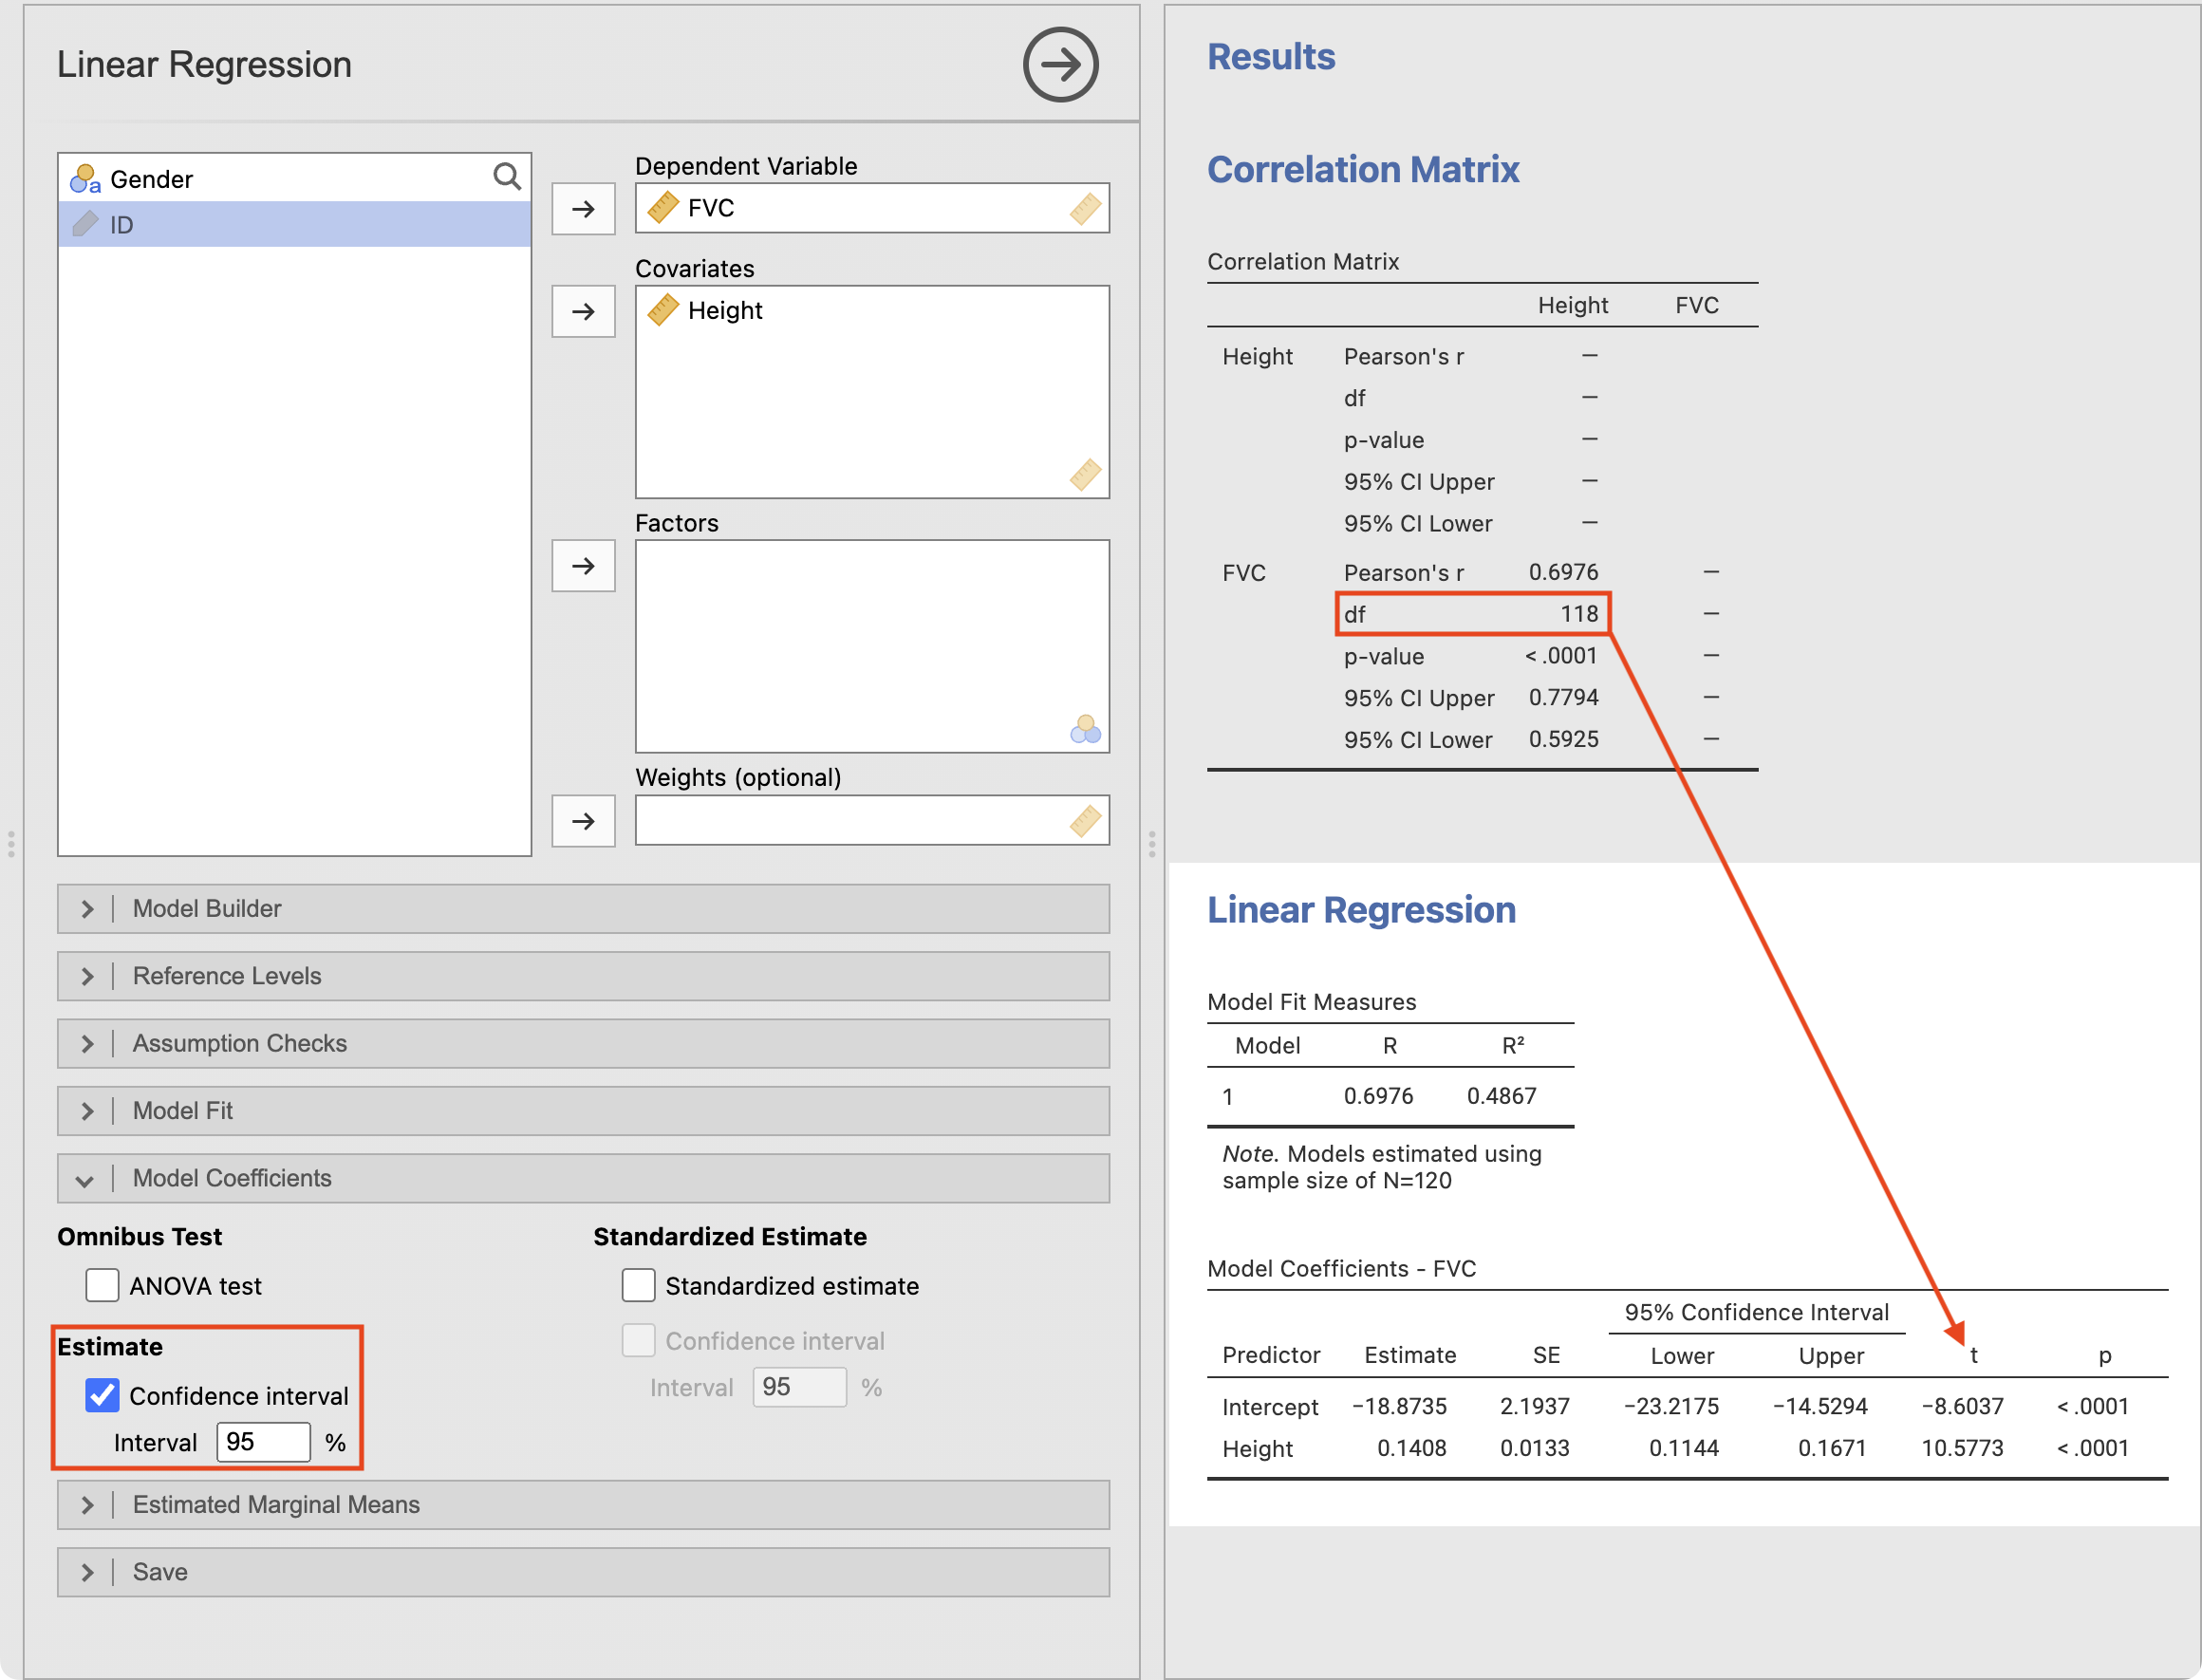
\includegraphics[width=0.8\linewidth,height=\textheight,keepaspectratio]{img/mod08/jamovi/regr-1.png}

You will notice that the Jamovi output does not provide the degrees of
freedom for the regression coefficient t-statistic. This is equivalent
to the degrees of freedom in the preceding correlation matrix: in this
case, 118 df.

\section{Plotting residuals from a simple linear
regression}\label{plotting-residuals-from-a-simple-linear-regression}

To plot the residuals, we first need to save them using the
\textbf{Save} option within the \textbf{Linear Regression} command box:

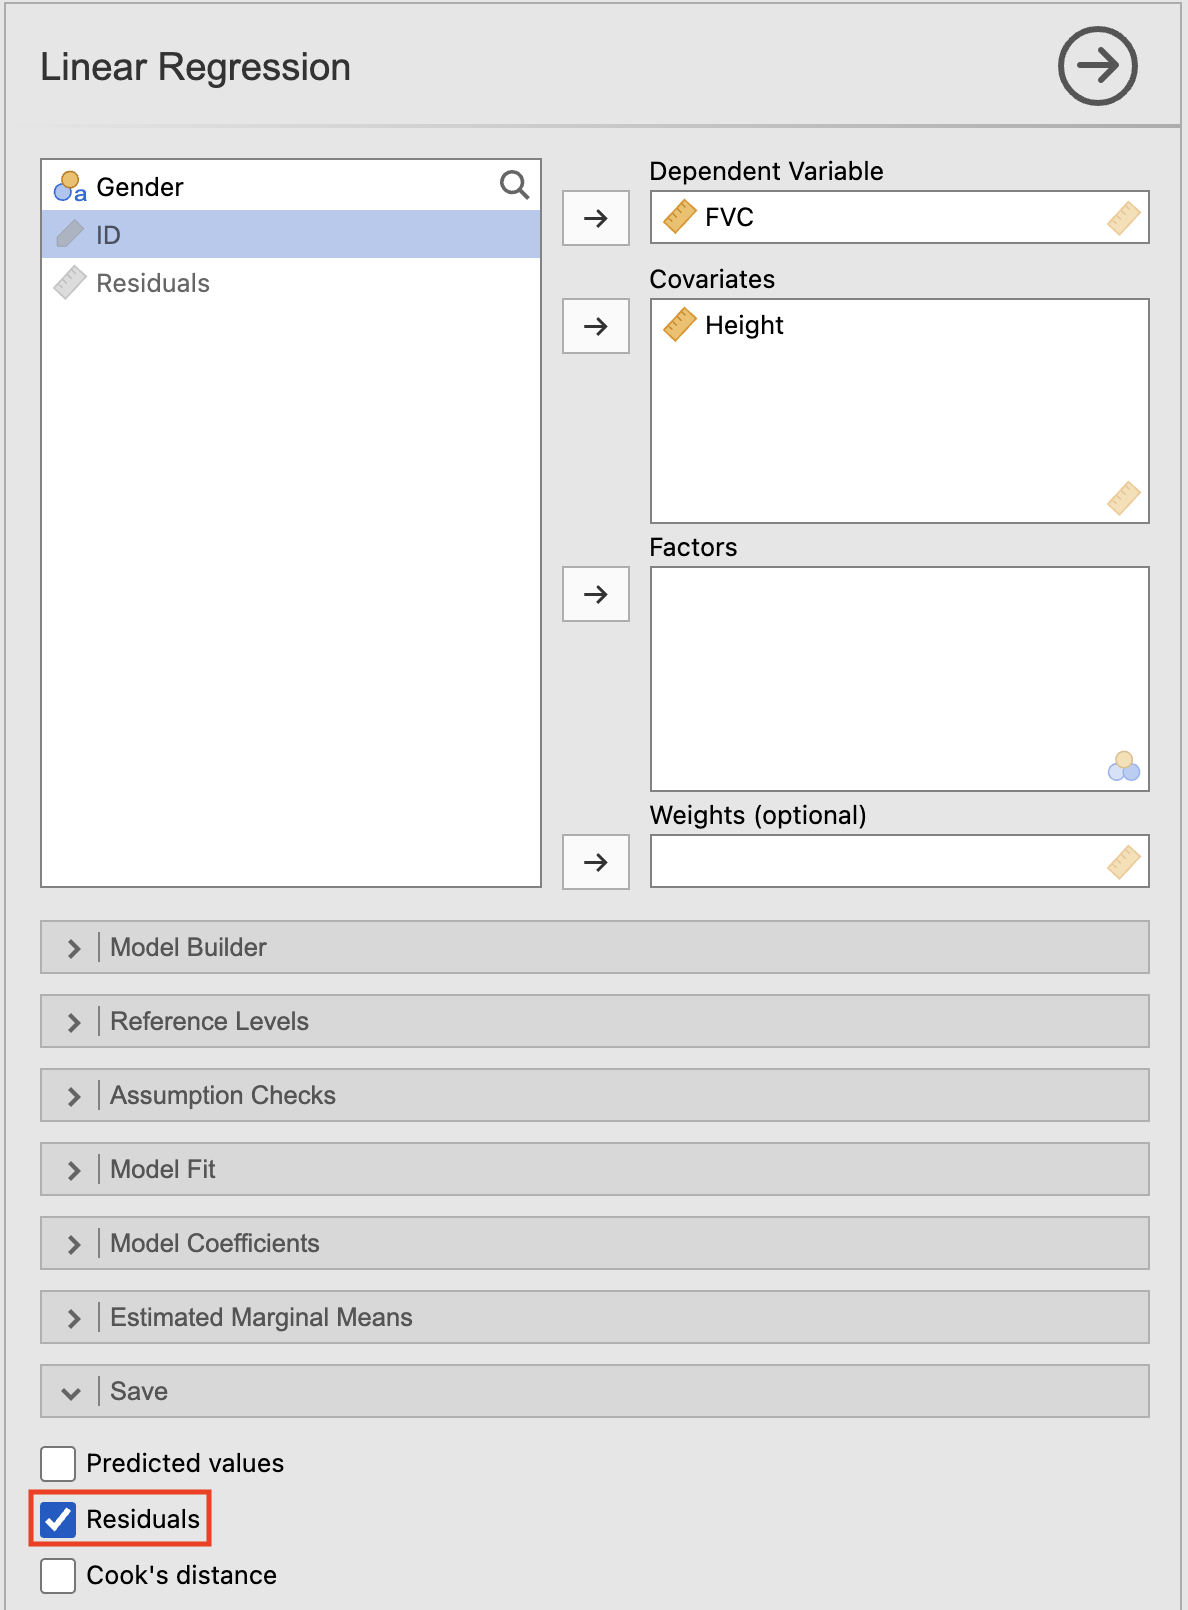
\includegraphics[width=0.8\linewidth,height=\textheight,keepaspectratio]{img/mod08/jamovi/resid-1.png}

This creates a new column of \emph{Residuals} within our dataset:

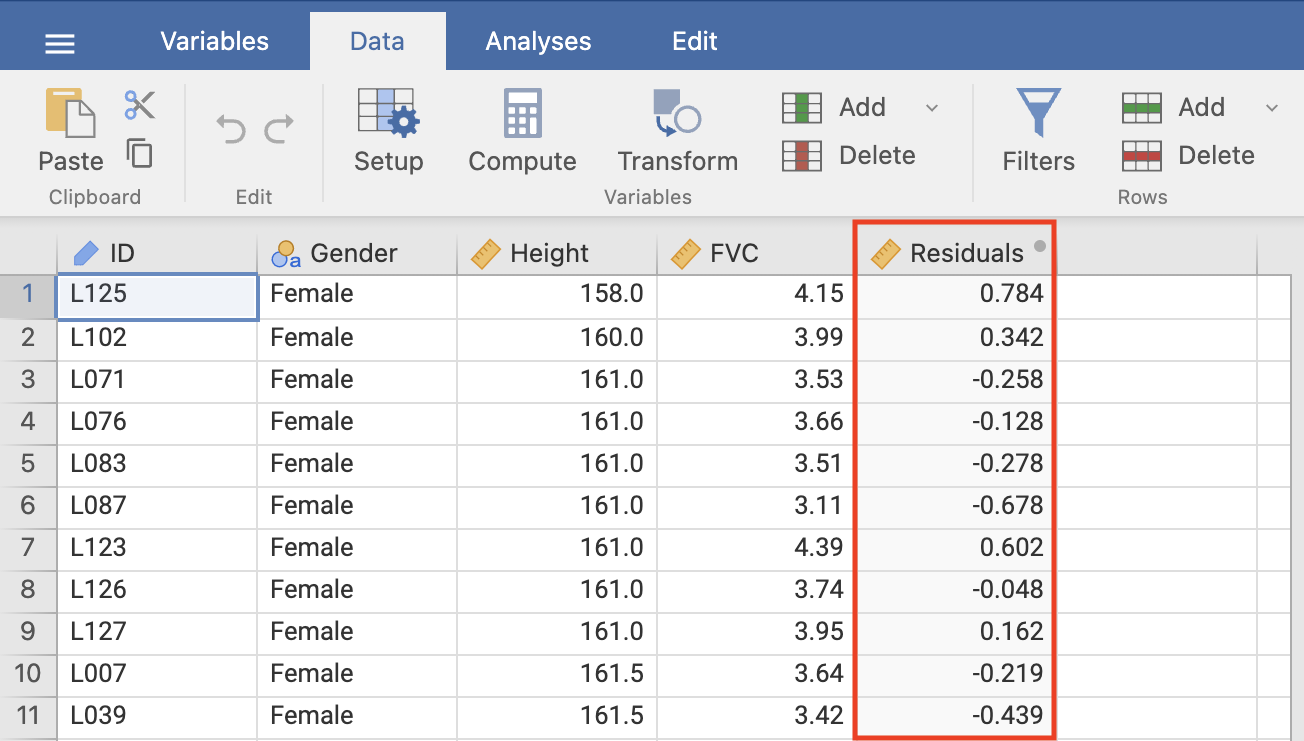
\includegraphics[width=0.8\linewidth,height=\textheight,keepaspectratio]{img/mod08/jamovi/resid-2.png}

You can now check the assumption that the residuals are normally
distributed by creating a density plot of the residuals using
\textbf{Exploration \textgreater{} Descriptives}, as shown in
Figure~\ref{fig-residual-dist}.

\newpage{}

\bookmarksetup{startatroot}

\chapter*{R notes}\label{r-notes-6}
\addcontentsline{toc}{chapter}{R notes}

\markboth{R notes}{R notes}

We will demonstrate using R for correlation and simple linear regression
using the dataset \texttt{mod08\_lung\_function.csv}.

\begin{Shaded}
\begin{Highlighting}[]
\NormalTok{lung }\OtherTok{\textless{}{-}} \FunctionTok{read.csv}\NormalTok{(}\StringTok{"data/examples/mod08\_lung\_function.csv"}\NormalTok{)}
\end{Highlighting}
\end{Shaded}

\section{Creating a scatter plot}\label{creating-a-scatter-plot-1}

We can use the \texttt{plot} function to create a scatter plot to
explore the association between height and FVC, assigning meaningful
labels with the \texttt{xlab} and \texttt{ylab} commands:

\begin{Shaded}
\begin{Highlighting}[]
\FunctionTok{plot}\NormalTok{(}\AttributeTok{x=}\NormalTok{lung}\SpecialCharTok{$}\NormalTok{Height, }\AttributeTok{y=}\NormalTok{lung}\SpecialCharTok{$}\NormalTok{FVC, }
     \AttributeTok{xlab=}\StringTok{"Height (cm)"}\NormalTok{, }
     \AttributeTok{ylab=}\StringTok{"Forced vital capacity (L)"}\NormalTok{)}
\end{Highlighting}
\end{Shaded}

\pandocbounded{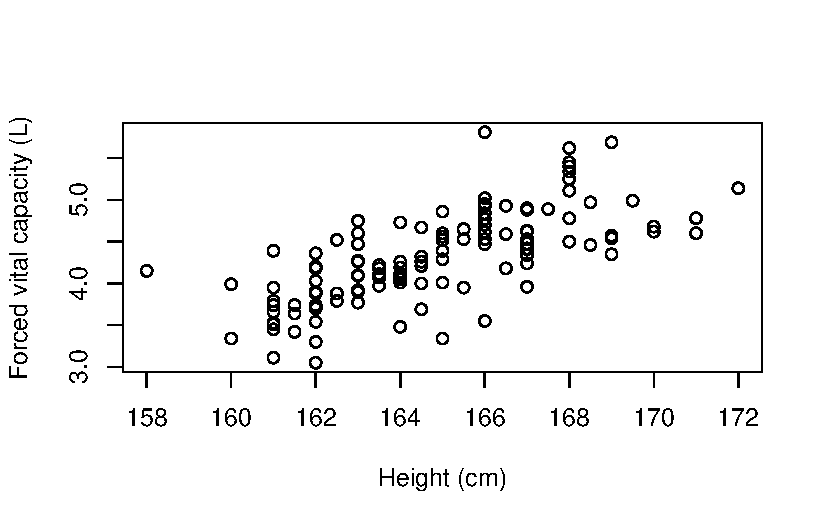
\includegraphics[keepaspectratio]{08-correlation-and-regression_files/figure-pdf/unnamed-chunk-4-1.pdf}}

To add a fitted line, we can use the \texttt{abline()} function which
adds a straight line to the plot. The equation of this straight line
will be determined from the estimated regression line, which we specify
with the \texttt{lm()} function, which fits a \emph{linear model}.

The basic syntax of the \texttt{lm()} function is:
\texttt{lm(y\ \textasciitilde{}\ x)} where \texttt{y} represents the
\emph{outcome} variable, and \texttt{x} represents the
\emph{explanatory} variable. Putting this all together:

\begin{Shaded}
\begin{Highlighting}[]
\FunctionTok{plot}\NormalTok{(}\AttributeTok{x=}\NormalTok{lung}\SpecialCharTok{$}\NormalTok{Height, }\AttributeTok{y=}\NormalTok{lung}\SpecialCharTok{$}\NormalTok{FVC,}
     \AttributeTok{xlab=}\StringTok{"Height (cm)"}\NormalTok{,}
     \AttributeTok{ylab=}\StringTok{"Forced vital capacity (L)"}\NormalTok{)}

\FunctionTok{abline}\NormalTok{(}\FunctionTok{lm}\NormalTok{(lung}\SpecialCharTok{$}\NormalTok{FVC }\SpecialCharTok{\textasciitilde{}}\NormalTok{ lung}\SpecialCharTok{$}\NormalTok{Height))}
\end{Highlighting}
\end{Shaded}

\pandocbounded{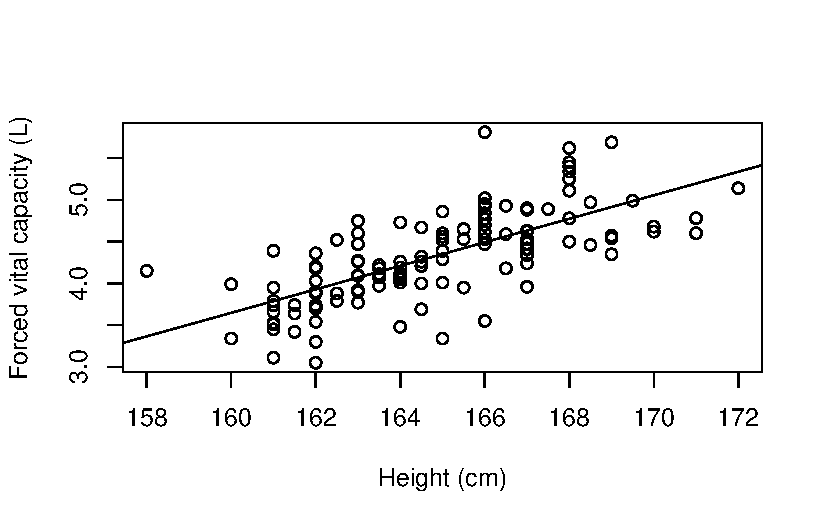
\includegraphics[keepaspectratio]{08-correlation-and-regression_files/figure-pdf/unnamed-chunk-5-1.pdf}}

Note: to obtain output similar to Jamovi output, we can use the
\texttt{scatr} package:

\begin{Shaded}
\begin{Highlighting}[]
\CommentTok{\# Install scatr if required:}
\CommentTok{\# install.packages("scatr")}
\FunctionTok{library}\NormalTok{(scatr)}

\FunctionTok{scat}\NormalTok{(}\AttributeTok{data=}\NormalTok{lung, }\AttributeTok{x=}\StringTok{"Height"}\NormalTok{, }\AttributeTok{y=}\StringTok{"FVC"}\NormalTok{, }\AttributeTok{line=}\StringTok{"linear"}\NormalTok{)}
\end{Highlighting}
\end{Shaded}

\pandocbounded{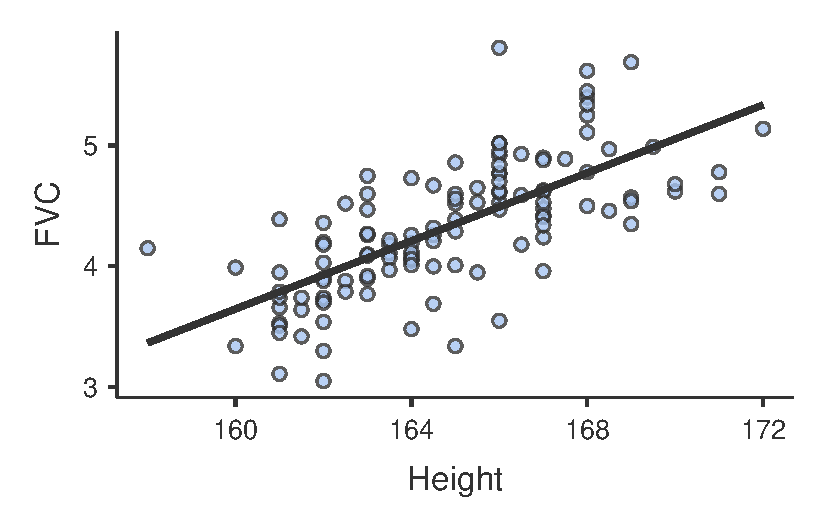
\includegraphics[keepaspectratio]{08-correlation-and-regression_files/figure-pdf/unnamed-chunk-6-1.pdf}}

Or using \texttt{ggplot2}, we use \texttt{geom\_point} to plot each
point defined by \texttt{x} and \texttt{y}:

\begin{Shaded}
\begin{Highlighting}[]
\FunctionTok{library}\NormalTok{(ggplot2)}

\FunctionTok{ggplot}\NormalTok{(}\AttributeTok{data=}\NormalTok{lung, }\FunctionTok{aes}\NormalTok{(}\AttributeTok{x=}\NormalTok{Height, }\AttributeTok{y=}\NormalTok{FVC)) }\SpecialCharTok{+}
  \FunctionTok{geom\_point}\NormalTok{() }\SpecialCharTok{+}
  \FunctionTok{theme\_classic}\NormalTok{() }\SpecialCharTok{+}
  \FunctionTok{labs}\NormalTok{(}\AttributeTok{x=}\StringTok{"Height (cm)"}\NormalTok{, }\AttributeTok{y=}\StringTok{"Forced vital capacity (L)"}\NormalTok{)}
\end{Highlighting}
\end{Shaded}

\pandocbounded{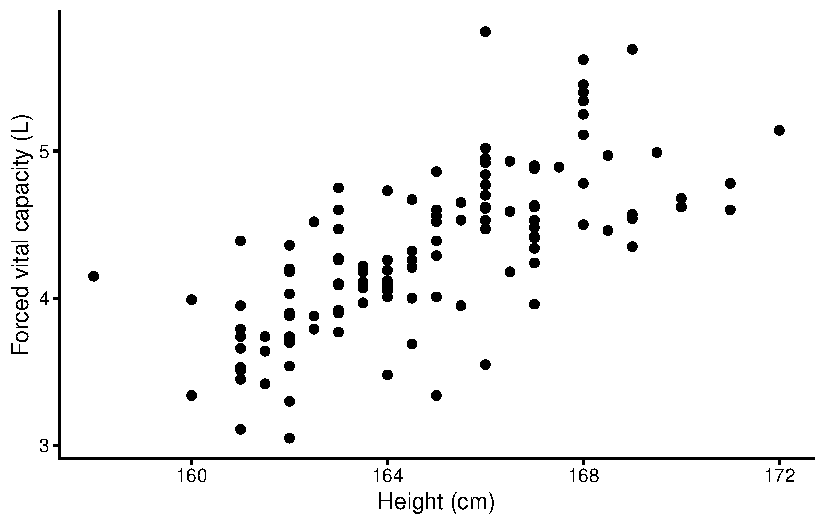
\includegraphics[keepaspectratio]{08-correlation-and-regression_files/figure-pdf/unnamed-chunk-7-1.pdf}}

We use \texttt{geom\_smooth()} to add a regression line. This geometry
``smooths'' your data, essentially drawing a smooth line through the
middle of the data. We specify that we want a line based on a linear
regression (i.e.~a \textbf{l}inear \textbf{m}odel) by including
\texttt{method=\textquotesingle{}ml\textquotesingle{}}, and we prevent a
shaded representation of the standard error of the regression by
including \texttt{se=FALSE}:

\begin{Shaded}
\begin{Highlighting}[]
\FunctionTok{ggplot}\NormalTok{(}\AttributeTok{data=}\NormalTok{lung, }\FunctionTok{aes}\NormalTok{(}\AttributeTok{x=}\NormalTok{Height, }\AttributeTok{y=}\NormalTok{FVC)) }\SpecialCharTok{+}
  \FunctionTok{geom\_point}\NormalTok{() }\SpecialCharTok{+}
  \FunctionTok{geom\_smooth}\NormalTok{(}\AttributeTok{method=}\StringTok{"lm"}\NormalTok{, }\AttributeTok{se=}\ConstantTok{FALSE}\NormalTok{) }\SpecialCharTok{+}
  \FunctionTok{theme\_classic}\NormalTok{() }\SpecialCharTok{+}
  \FunctionTok{labs}\NormalTok{(}\AttributeTok{x=}\StringTok{"Height (cm)"}\NormalTok{, }\AttributeTok{y=}\StringTok{"Forced vital capacity (L)"}\NormalTok{)}
\end{Highlighting}
\end{Shaded}

\pandocbounded{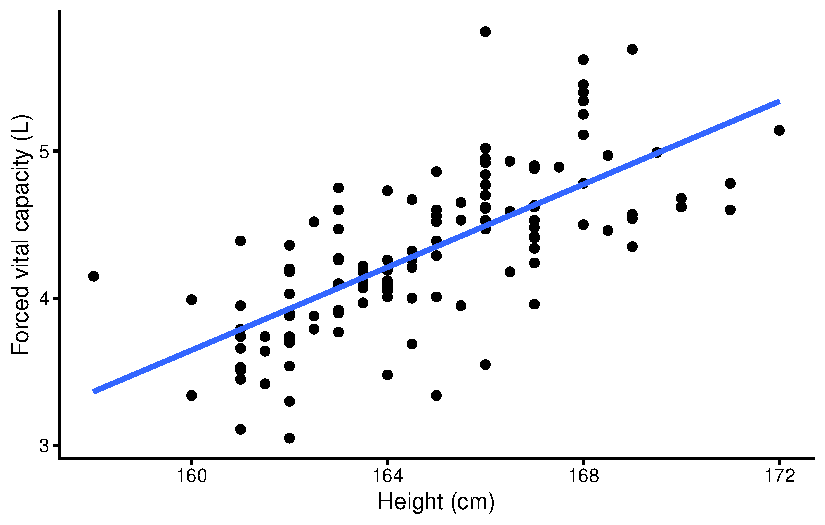
\includegraphics[keepaspectratio]{08-correlation-and-regression_files/figure-pdf/unnamed-chunk-8-1.pdf}}

\section*{Calculating a correlation
coefficient}\label{calculating-a-correlation-coefficient-1}
\addcontentsline{toc}{section}{Calculating a correlation coefficient}

\markright{Calculating a correlation coefficient}

We can use the \texttt{corrMatrix} function in the Jamovi package to
calculate a Pearson's correlation coefficient with a 95\% confidence
interval:

\begin{Shaded}
\begin{Highlighting}[]
\FunctionTok{corrMatrix}\NormalTok{(}\AttributeTok{data=}\NormalTok{lung, }\AttributeTok{vars=}\FunctionTok{c}\NormalTok{(Height, FVC), }\AttributeTok{ci=}\ConstantTok{TRUE}\NormalTok{)}
\end{Highlighting}
\end{Shaded}

\begin{verbatim}

 CORRELATION MATRIX

 Correlation Matrix                                    
 ───────────────────────────────────────────────────── 
                             Height        FVC         
 ───────────────────────────────────────────────────── 
   Height    Pearson's r              —                
             df                       —                
             p-value                  —                
             95% CI Upper             —                
             95% CI Lower             —                
                                                       
   FVC       Pearson's r      0.6976279            —   
             df                     118            —   
             p-value         < .0000001            —   
             95% CI Upper     0.7794090            —   
             95% CI Lower     0.5924715            —   
 ───────────────────────────────────────────────────── 
\end{verbatim}

\section{Fitting a simple linear regression
model}\label{fitting-a-simple-linear-regression-model-1}

We can use the \texttt{lm} function to fit a simple linear regression
model, specifying the model as \texttt{y\ \textasciitilde{}\ x} where
\texttt{y} represents the \emph{outcome} variable, and \texttt{x}
represents the \emph{explanatory} variable. Using
\texttt{mod08\_lung\_function.csv}, we can quantify the relationship
between FVC and height:

\begin{Shaded}
\begin{Highlighting}[]
\FunctionTok{lm}\NormalTok{(FVC }\SpecialCharTok{\textasciitilde{}}\NormalTok{ Height, }\AttributeTok{data=}\NormalTok{lung)}
\end{Highlighting}
\end{Shaded}

\begin{verbatim}

Call:
lm(formula = FVC ~ Height, data = lung)

Coefficients:
(Intercept)       Height  
   -18.8735       0.1408  
\end{verbatim}

The default output from the \texttt{lm} function is rather sparse. We
can obtain much more useful information by defining the linear
regression model as an object, then using the \texttt{summary()}
function:

\begin{Shaded}
\begin{Highlighting}[]
\NormalTok{model }\OtherTok{\textless{}{-}} \FunctionTok{lm}\NormalTok{(FVC }\SpecialCharTok{\textasciitilde{}}\NormalTok{ Height, }\AttributeTok{data=}\NormalTok{lung)}
\FunctionTok{summary}\NormalTok{(model)}
\end{Highlighting}
\end{Shaded}

\begin{verbatim}

Call:
lm(formula = FVC ~ Height, data = lung)

Residuals:
     Min       1Q   Median       3Q      Max 
-1.01139 -0.23643 -0.02082  0.24918  1.31786 

Coefficients:
             Estimate Std. Error t value Pr(>|t|)    
(Intercept) -18.87347    2.19365  -8.604 3.89e-14 ***
Height        0.14076    0.01331  10.577  < 2e-16 ***
---
Signif. codes:  0 '***' 0.001 '**' 0.01 '*' 0.05 '.' 0.1 ' ' 1

Residual standard error: 0.3965 on 118 degrees of freedom
Multiple R-squared:  0.4867,    Adjusted R-squared:  0.4823 
F-statistic: 111.9 on 1 and 118 DF,  p-value: < 2.2e-16
\end{verbatim}

Finally, we can obtain 95\% confidence intervals for the regression
coefficients using the \texttt{confint} function:

\begin{Shaded}
\begin{Highlighting}[]
\FunctionTok{confint}\NormalTok{(model)}
\end{Highlighting}
\end{Shaded}

\begin{verbatim}
                  2.5 %      97.5 %
(Intercept) -23.2174967 -14.5294441
Height        0.1144042   0.1671092
\end{verbatim}

Note that the output for R looks slightly different from the Jamovi
output, the numerical values are identical.

\section{Plotting residuals from a simple linear
regression}\label{plotting-residuals-from-a-simple-linear-regression-1}

We can use the \texttt{resid} function to obtain the residuals from a
saved model. These residuals can then be plotted using a density plot in
the usual way:

\begin{Shaded}
\begin{Highlighting}[]
\NormalTok{residuals }\OtherTok{\textless{}{-}} \FunctionTok{resid}\NormalTok{(model)}
\FunctionTok{plot}\NormalTok{(}\FunctionTok{density}\NormalTok{(residuals))}
\end{Highlighting}
\end{Shaded}

\pandocbounded{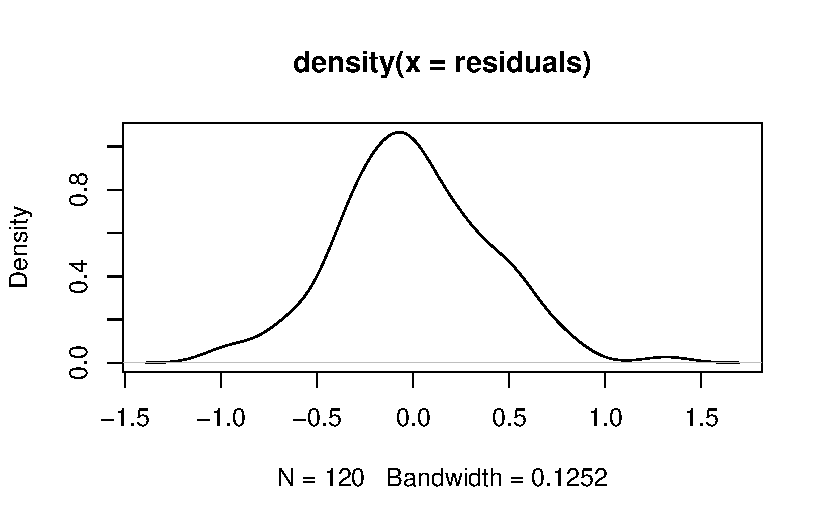
\includegraphics[keepaspectratio]{08-correlation-and-regression_files/figure-pdf/unnamed-chunk-13-1.pdf}}

\newpage{}

\bookmarksetup{startatroot}

\chapter*{Activities}\label{activities-7}
\addcontentsline{toc}{chapter}{Activities}

\markboth{Activities}{Activities}

\subsection*{Activity 8.1}\label{activity-8.1}
\addcontentsline{toc}{subsection}{Activity 8.1}

To investigate how body weight (kg) effects blood plasma volume (mL),
data were collected from 30 participants and a simple linear regression
analysis was conducted. The slope of the regression was 68 (95\%
confidence interval 52 to 84) and the intercept was −1570 (95\%
confidence interval −2655 to −492).

{[}\emph{You do not need software for this Activity}{]}

\begin{enumerate}
\def\labelenumi{\alph{enumi})}
\tightlist
\item
  What is the outcome variable and explanatory (exposure) variable?
\item
  Interpret the regression slope and its 95\% CI
\item
  Write the regression equation
\item
  If we randomly sampled a person from the population and found that
  their weight is 80kg, what would be the predicted value of plasma
  volume for this person?
\end{enumerate}

\subsection*{Activity 8.2}\label{activity-8.2}
\addcontentsline{toc}{subsection}{Activity 8.2}

To examine whether age predicts IQ, data were collected on 104 people.
Use the data in the file \texttt{Activity\_8.2.rds} to answer the
following questions.

\begin{enumerate}
\def\labelenumi{\alph{enumi})}
\tightlist
\item
  What is the outcome variable and the explanatory variable?
\item
  Create a scatter plot with the two variables. What can you infer from
  the scatter plot?
\item
  Obtain the correlation coefficient between age and IQ and interpret
  it.
\item
  Conduct a simple linear regression and report the relationship between
  the two variables including the interpretation of the
  R\textsuperscript{2} value. Are the assumptions for linear regression
  met in this model?
\item
  What could you infer about the association between age and IQ in the
  population, based on the results of the regression analysis in this
  sample?
\end{enumerate}

\subsection*{Activity 8.3}\label{activity-8.3}
\addcontentsline{toc}{subsection}{Activity 8.3}

Which of the following correlation coefficients indicates the weakest
linear relationship and why?

\begin{enumerate}
\def\labelenumi{\alph{enumi})}
\tightlist
\item
  r = 0.72
\item
  r = 0.41
\item
  r = 0.13
\item
  r = −0.33
\item
  r = −0.84
\end{enumerate}

\subsection*{Activity 8.4}\label{activity-8.4}
\addcontentsline{toc}{subsection}{Activity 8.4}

Are the following statements true or false?

\begin{enumerate}
\def\labelenumi{\alph{enumi})}
\tightlist
\item
  If a correlation coefficient is closer to 1.00 than to 0.00, this
  indicates that the outcome is caused by the exposure.
\item
  If a researcher has data on two variables, there will be a higher
  correlation if the two means are close together and a lower
  correlation if the two means are far apart.
\end{enumerate}

\subsection*{Supplementary Activity
8.5}\label{supplementary-activity-8.5}
\addcontentsline{toc}{subsection}{Supplementary Activity 8.5}

A cross-sectional study was conducted to examine the association between
gestational age and systolic blood pressure in low birthweight babies.
Data were collected at birth from 60 low birthweight babies and saved in
the file \texttt{Activity\_8.5\_babies.csv}. The dataset contains the
following variables:

\begin{itemize}
\tightlist
\item
  ID: participant ID number
\item
  sbp: systolic blood pressure (mmHg)
\item
  gestage: gestational age (weeks)
\end{itemize}

In this analysis, the researchers are interested in assessing the
association between systolic blood pressure (the outcome variable) and
gestational age (the explanatory variable).

NOTE: there is no need to apply clinical knowledge to the values of
systolic blood pressure.

\begin{enumerate}
\def\labelenumi{\alph{enumi})}
\tightlist
\item
  Produce a scatter plot summarising the relationship between systolic
  blood pressure and gestational age, and describe this relationship.
\item
  Estimate the correlation coefficient between systolic blood pressure
  and gestational age, and interpret it.
\item
  Fit a simple linear regression model predicting systolic blood
  pressure from gestational age, and present the estimated regression
  equation.
\item
  Are the assumptions of simple linear regression satisfied for your
  regression model? Provide evidence to support your claim.
\item
  Summarise your regression model in a brief conclusion.
\end{enumerate}

\bookmarksetup{startatroot}

\chapter{Analysing non-normal data}\label{analysing-non-normal-data}

\section*{Learning objectives}\label{learning-objectives-8}
\addcontentsline{toc}{section}{Learning objectives}

\markright{Learning objectives}

By the end of this module you will be able to:

\begin{itemize}
\tightlist
\item
  Transform non-normally distributed variables;
\item
  Explain the purpose of non-parametric statistics and key principles
  for their use;
\item
  Calculate ranks for variables;
\item
  Conduct and interpret a non-parametric independent samples
  significance test;
\item
  Conduct and interpret a non-parametric paired samples significance
  test;
\item
  Calculate and interpret the Spearman rank correlation coefficient.
\end{itemize}

\section*{Optional readings}\label{optional-readings-8}
\addcontentsline{toc}{section}{Optional readings}

\markright{Optional readings}

Kirkwood and Sterne (2001); Chapter 13.
\href{http://er1.library.unsw.edu.au/er/cgi-bin/eraccess.cgi?url=https://ebookcentral.proquest.com/lib/unsw/detail.action?docID=624728}{{[}UNSW
Library Link{]}}

Bland (2015); Chapter 12.
\href{http://er1.library.unsw.edu.au/er/cgi-bin/eraccess.cgi?url=https://ebookcentral.proquest.com/lib/unsw/detail.action?docID=5891730}{{[}UNSW
Library Link{]}}

\section{Introduction}\label{introduction-8}

In general, parametric statistics are preferred for reporting data
because the summary statistics (mean, standard deviation, standard error
of the mean etc) and the tests used (t-tests, correlation, regression
etc) are familiar and the results are easy to communicate. However,
non-parametric tests can be used if data are not normally distributed.
Non-parametric tests make fewer assumptions about the distribution of
the data.

\section{Transforming non-normally distributed
variables}\label{transforming-non-normally-distributed-variables}

When a variable has a skewed distribution, one possibility is to
transform the data to a new variable to try and obtain a normal or near
normal distribution. Methods to transform non-normally distributed data
include logarithmic transformation of each data point, or using the
square root or the square or the inverse (i.e.~1/x) etc.

\subsection{Worked Example}\label{worked-example-6}

We have data from 132 patients who had a hospital stay following
admission to ICU (\texttt{mod09\_infection.rds}). The distribution of
the length of stay for these patients is shown in the density plot in
Figure~\ref{fig-mod09-los}. As is common with variables that record
time, the data are skewed with many patients having relatively short
stays and a few patients having very long hospital stays. Clearly, it
would be inappropriate to use parametric statistical methods for these
data.

\begin{figure}

\centering{

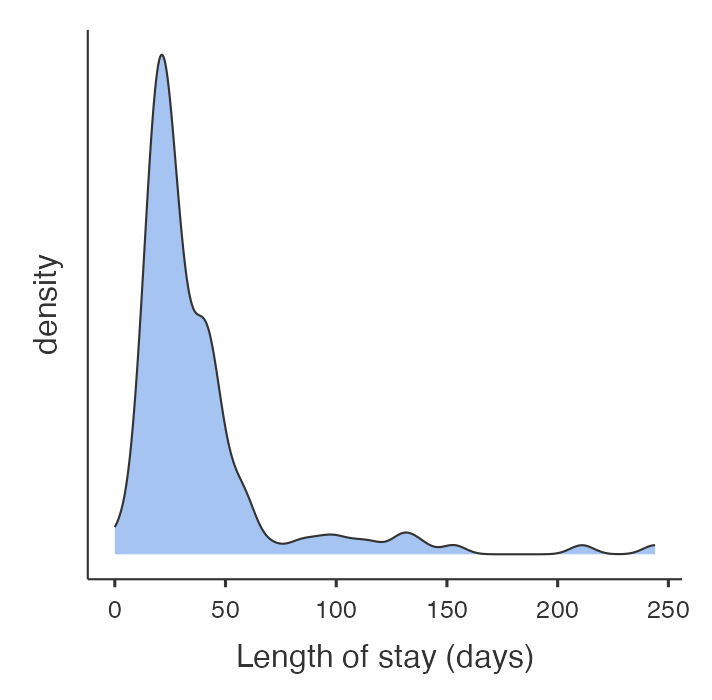
\includegraphics[width=0.66\linewidth,height=\textheight,keepaspectratio]{img/mod09/mod09-los-dist.png}

}

\caption{\label{fig-mod09-los}Length of hospital stay for 132 patients}

\end{figure}%

When data are positively skewed, as shown in Figure~\ref{fig-mod09-los},
a logarithmic transformation can often make the data closer to being
normally distributed. This is the most common transformation used. You
should note, however, that the logarithmic function cannot handle 0 or
negative values. One way to deal with zeros in a set of data is to add 1
to each value before taking the logarithm.

We would generate a new variable, as shown in the jamovi or R notes. As
the minimum length of stay in these sample data was 0, we have added 1
to each length of stay before taking the logarithm. The distribution of
the logarithm of (length of stay + 1) is shown in
Figure~\ref{fig-mod09-lnlos}.

\begin{figure}

\centering{

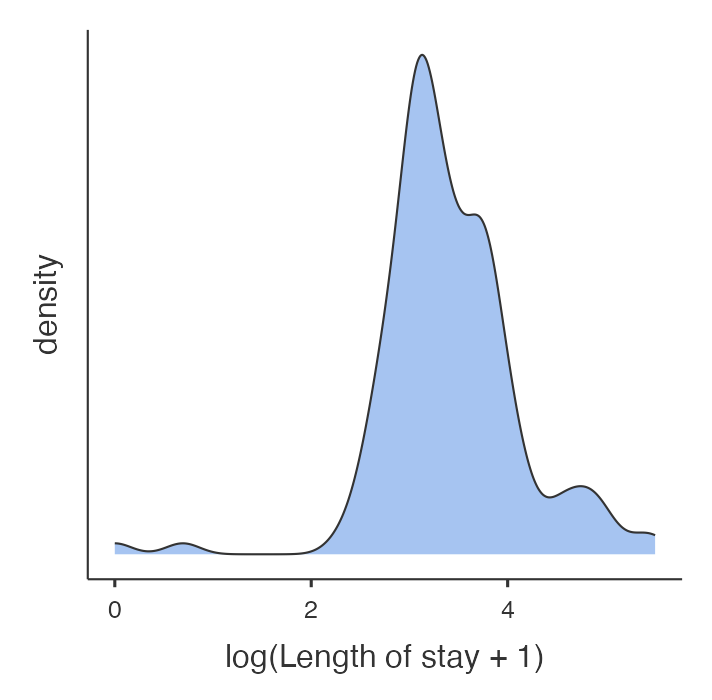
\includegraphics[width=0.66\linewidth,height=\textheight,keepaspectratio]{img/mod09/mod09-lnlos-dist.png}

}

\caption{\label{fig-mod09-lnlos}Distribution of log transformed (length
of stay + 1)}

\end{figure}%

The distribution now appears much more bell shaped.
Table~\ref{tbl-los-desc} shows the descriptive statistics for length of
stay before and after logarithmic transformation. Before transformation,
the SD is almost as large as the mean value which indicates that the
data are skewed and that these statistics are not an accurate
description of the centre and spread of the data.

\begin{longtable}[]{@{}
  >{\raggedright\arraybackslash}p{(\linewidth - 4\tabcolsep) * \real{0.4324}}
  >{\raggedright\arraybackslash}p{(\linewidth - 4\tabcolsep) * \real{0.2297}}
  >{\raggedright\arraybackslash}p{(\linewidth - 4\tabcolsep) * \real{0.3378}}@{}}
\caption{Summary statistics for untransformed and transformed length of
stay}\label{tbl-los-desc}\tabularnewline
\toprule\noalign{}
\begin{minipage}[b]{\linewidth}\raggedright
\end{minipage} & \begin{minipage}[b]{\linewidth}\raggedright
Length of stay
\end{minipage} & \begin{minipage}[b]{\linewidth}\raggedright
log(Length of stay + 1)
\end{minipage} \\
\midrule\noalign{}
\endfirsthead
\toprule\noalign{}
\begin{minipage}[b]{\linewidth}\raggedright
\end{minipage} & \begin{minipage}[b]{\linewidth}\raggedright
Length of stay
\end{minipage} & \begin{minipage}[b]{\linewidth}\raggedright
log(Length of stay + 1)
\end{minipage} \\
\midrule\noalign{}
\endhead
\bottomrule\noalign{}
\endlastfoot
Mean (Standard deviation) & 38.1 (35.78) & 3.41 (0.715) \\
Mean: 95\% confidence interval & 31.9 to 44.2 & 3.29 to 3.53 \\
Median {[}Interquartile range{]} & 27 {[}21 to 42{]} & 3.3 {[}3.1 to
3.8{]} \\
Range & 0 to 244 & 0 to 5.5 \\
\end{longtable}

The mean and standard deviation of the transformed length of stay are in
log base e (i.e.~ln) units. If we raise the mean of the log of length of
stay to the power of \(e\), it returns a value of 30.2 days
(\(e^{3.41}=30.2\)).

Technically, this is called the geometric mean of the data, and it has a
different interpretation to the usual mean, the arithmetic mean. This is
a much better estimate in this case of the ``average'' length of stay
than the mean of 38.1 days (95\% CI 31.9, 44.2 days) obtained from the
non-transformed positively skewed data. Note that, if you have added 1
to your data to deal with 0 values, the back-transformed estimate is
\emph{approximately} equal to the geometric mean.

This set of data also includes a variable summarising whether a patient
acquired a nosocomial infection (also known as healthcare-associated
infections), which are infections that develop while undergoing medical
treatment but were absent at the time of admission.

If we were testing the hypothesis that there was a difference in length
of stay between groups (status of nosocomial infection), t-tests should
not be used with length of stay, but could be used for the log
transformed variable, which is approximately normally distributed. The
output from the t-test of the log-transformed length of stay is shown in
Table~\ref{tbl-los-ttest}. This is done using the t-test shown in Module
5.

\begin{longtable}[]{@{}lllc@{}}
\caption{Summary statistics for transformed length of
stay}\label{tbl-los-ttest}\tabularnewline
\toprule\noalign{}
Nosocomial infection & n & Mean (SE) & 95\% Confidence interval \\
\midrule\noalign{}
\endfirsthead
\toprule\noalign{}
Nosocomial infection & n & Mean (SE) & 95\% Confidence interval \\
\midrule\noalign{}
\endhead
\bottomrule\noalign{}
\endlastfoot
No & 106 & 3.33 (0.068) & 3.19 to 3.46 \\
Yes & 26 & 3.73 (0.136) & 3.45 to 4.01 \\
Difference (Yes - No) & & 0.39 (0.153) & 0.09 to 0.70 \\
\end{longtable}

Here, a two-sample t-test gives a test statistic of -2.61 with 38.5
degrees of freedom, and a P-value of 0.01.

As explained above, the estimated statistics would need to be converted
back to the units in which the variable was measured. From
Table~\ref{tbl-los-ttest}, we can take the exponential of the
corresponding log-transformed values:

\begin{itemize}
\tightlist
\item
  the geometric mean of the infected group is approximately 41.5 days
  with a 95\% confidence interval from 31.4 to 55.0 days.
\item
  the geometric mean of the uninfected group is approximately 27.9 days
  with a 95\% confidence interval from 24.4 to 31.9 days.
\end{itemize}

\section{Non-parametric significance
tests}\label{non-parametric-significance-tests}

It is often not possible or sensible to transform a non-normal
distribution, for example if there are too many zero values or when we
simply want to compare groups using the unit in which the measurement
was taken (e.g.~length of stay). For this, non-parametric significance
tests can be used but the general idea behind these tests is that the
data values are replaced by ranks. This also protects against outliers
having too much influence.

\subsection{Ranking variables}\label{ranking-variables}

Table~\ref{tbl-9-1} shows how ranks are calculated for the first 21
patients in the length-of-stay data. First the data are sorted in order
of their magnitude (from the lowest value to the highest) ignoring the
group variable. Each data point is then assigned a rank. Data points
that are equal are assigned the mean of their ranks. Thus, the two
lengths of stay of 11 days share the ranks 4 and 5, and have a mean rank
of 4.5. Similarly, there are 5 people with a length of stay of 14 days
and these share the ranks 9 to 13, the mean of which is 11. Once ranks
are computed they are assigned to each of the two groups and summed
within each group.

\begin{table}

\caption{\label{tbl-9-1}Transforming data to ranks (first 21
participants)}

\centering{

\centering
\begin{tblr}[         %% tabularray outer open
]                     %% tabularray outer close
{                     %% tabularray inner open
colspec={Q[]Q[]Q[]Q[]Q[]Q[]},
hline{2}={1-6}{solid, black, 0.05em},
hline{1}={1-6}{solid, black, 0.08em},
hline{23}={1-6}{solid, black, 0.08em},
}                     %% tabularray inner close
ID & Infection & Length of stay & Rank & Infection=no & Infection=Yes \\
32 & No & 0 & 1.0 & 1.0 &   \\
33 & No & 1 & 2.0 & 2.0 &   \\
12 & No & 9 & 3.0 & 3.0 &   \\
22 & No & 11 & 4.5 & 4.5 &   \\
16 & No & 11 & 4.5 & 4.5 &   \\
28 & Yes & 12 & 6.0 &   & 6.0 \\
27 & No & 13 & 7.5 & 7.5 &   \\
20 & No & 13 & 7.5 & 7.5 &   \\
24 & No & 14 & 11.0 & 11.0 &   \\
11 & No & 14 & 11.0 & 11.0 &   \\
130 & No & 14 & 11.0 & 11.0 &   \\
10 & No & 14 & 11.0 & 11.0 &   \\
25 & No & 14 & 11.0 & 11.0 &   \\
19 & No & 15 & 15.5 & 15.5 &   \\
30 & No & 15 & 15.5 & 15.5 &   \\
23 & No & 15 & 15.5 & 15.5 &   \\
14 & No & 15 & 15.5 & 15.5 &   \\
15 & No & 17 & 20.5 & 20.5 &   \\
13 & No & 17 & 20.5 & 20.5 &   \\
21 & Yes & 17 & 20.5 &   & 20.5 \\
17 & No & 17 & 20.5 & 20.5 &   \\
\end{tblr}

}

\end{table}%

By assigning ranks to individuals, we lose information about their
actual values and this makes it more difficult to detect a difference.
However, outliers and extreme values in the data are brought back closer
to the data so that they are less influential. For this reason,
non-parametric tests have less power than parametric tests and they
require much larger differences in the data to show statistical
significance between groups.

\section{Non-parametric test for two independent samples (Wilcoxon
ranked sum
test)}\label{non-parametric-test-for-two-independent-samples-wilcoxon-ranked-sum-test}

The non-parametric equivalent to an independent samples t-test (Module
5) is the Wilcoxon ranked sum test, also known as the Mann-Whitney U
test. This can be obtained using the \texttt{Mann-Whitney\ U} option in
jamovi, and the \texttt{wilcox.test} in R.

The assumption for this test is that the distributions of the two
populations have the same general shape. If this assumption is met, then
this test evaluates the null hypothesis that the medians of the two
populations are equal. This test does not assume that the populations
are normally distributed, nor that their variances are equal.

Conducting the Wilcoxon ranked sum test for our length of stay data
yields a P-value of 0.014, providing evidence of a difference in the
median length of stay between the groups.

This P-value should be provided alongside non-parametric summary
statistics such as medians and inter-quartile ranges. In our example, we
can obtain the median length of stay values of 24 (Interquartile Range:
19 to 40 days) in the group with no infection and 37 (Interquartile
Range: 24 to 50 days) in the group with infection.

\section{Non-parametric test for paired data (Wilcoxon signed-rank
test)}\label{non-parametric-test-for-paired-data-wilcoxon-signed-rank-test}

There are two types of non-parametric tests for paired data, called the
Sign test and the Wilcoxon signed rank test. In practice, the Sign test
is rarely used and will not be discussed in this course.

If the differences between two paired measurements are not normally
distributed, a non-parametric equivalent of a paired t-test (Module 5)
should be used. The equivalent test is the Wilcoxon matched-pairs signed
rank test, also simply called the Wilcoxon matched-pairs test. This test
is resistant to outliers in the data, however the proportion of outliers
in the sample should be small. This test evaluates the null hypothesis
that the median of the paired differences is equal to zero.

In this test, the absolute differences between the paired scores are
ranked and the difference scores that are equal to zero (i.e.~scores
where there is no difference between the pairs) are excluded. Note that
the power of the test (the ability to detect an effect if there truly is
an effect) reduces in the presence of zero differences, as the effective
sample size (the number of non-zero differences) is reduced.

\subsection{Worked Example}\label{worked-example-7}

A crossover trial is done to compare symptom scores for two drugs in 11
people with arthritis (higher scores indicate more severe symptoms). The
data are contained in datafile file \texttt{mod09\_arthritis.csv}. The
data are shown in Table~\ref{tbl-9-2}.

\begin{table}

\caption{\label{tbl-9-2}Arthritis symptom scores for 11 patients after
administering two drugs}

\centering{

\centering
\begin{tblr}[         %% tabularray outer open
]                     %% tabularray outer close
{                     %% tabularray inner open
colspec={Q[]Q[]Q[]Q[]},
hline{2}={1-4}{solid, black, 0.05em},
hline{1}={1-4}{solid, black, 0.08em},
hline{13}={1-4}{solid, black, 0.08em},
}                     %% tabularray inner close
Patient ID & Score: Drug 1 & Score: Drug 2 & Difference (Drug 2 - Drug 1) \\
1 & 3 & 4 & 1 \\
2 & 2 & 7 & 5 \\
3 & 3 & 4 & 1 \\
4 & 8 & 10 & 2 \\
5 & 6 & 8 & 2 \\
6 & 6 & 1 & -5 \\
7 & 2 & 6 & 4 \\
8 & 3 & 7 & 4 \\
9 & 5 & 8 & 3 \\
10 & 9 & 10 & 1 \\
11 & 7 & 8 & 1 \\
\end{tblr}

}

\end{table}%

The data shows that there is 1 person who has a negative difference,
where the symptom score on drug 2 that is smaller than that for drug 1
(i.e., drug 2 is better than drug 1); and 10 people who have a positive
difference. No one has the same score for both drugs.

Before doing the analysis let us examine the distribution of the
difference of symptom scores between the two drugs. As in Module 5, we
first need to compute the difference between the symptom scores. To
examine the distribution, we construct a distribution plot as shown in
Figure~\ref{fig-mod09-diff-hist}.

\begin{figure}

\centering{

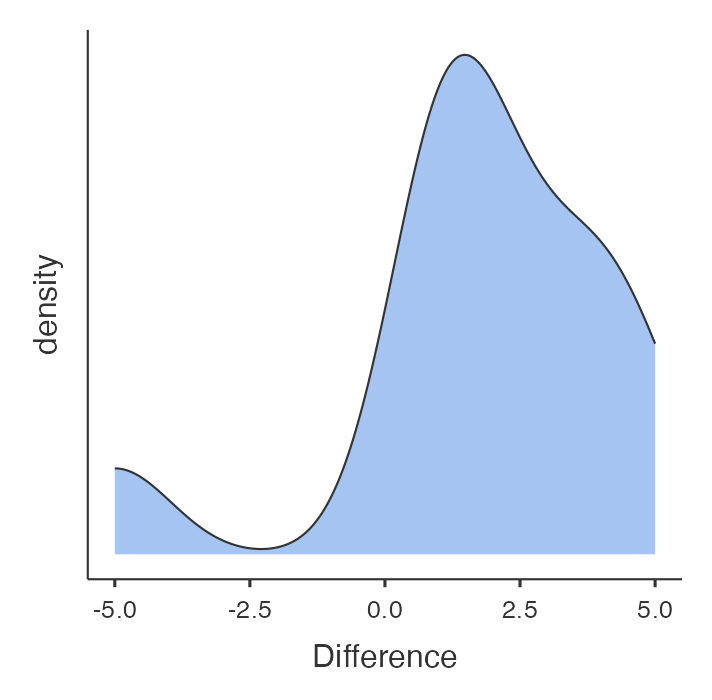
\includegraphics[width=0.66\linewidth,height=\textheight,keepaspectratio]{img/mod09/mod09-diff-dist.png}

}

\caption{\label{fig-mod09-diff-hist}Distribution of difference in
symptom scores between Drug 1 and Drug 2}

\end{figure}%

The plot shows that the differences are not normally distributed. The
data looks weirdly negatively skewed with a gap in values around -2.5.
Therefore, it would not be appropriate to conduct a paired t-test.
Hence, we conduct a non-parametric paired test (Wilcoxon matched-pairs
signed-rank test).

The P-value obtained from this test is 0.049. Thus, there is evidence of
a difference in symptom scores between the two drugs.

\section{Non-parametric estimates of
correlation}\label{non-parametric-estimates-of-correlation}

Estimating correlation using Pearson's correlation coefficient can be
problematic when bivariate Normality cannot be assumed, or in the
presence of outliers or skewness. One commonly used non-parametric
alternative to Pearson's correlation coefficient is the Spearman's rank
correlation (\(\rho\) or rho). When estimating the correlation between x
and y, Spearman's rank correlation essentially replaces the observations
x and y by their ranks, and calculates the correlation between the
ranks.

We will illustrate estimating rank correlation using the data
\texttt{mod08\_lung\_function.csv}, which has information about height
and lung function collected from a sample of 120 adults. The Spearman
rank correlation coefficient is estimated as 0.75, demonstrating a
positive association between height and FVC.

Kendall's tau (\(\tau\)) is an alternative to the Spearman rank
correlation, but it less commonly used.

\section{Summary}\label{summary-1}

In this module, we have presented methods to conduct a hypothesis test
with data that are not normally distributed. Non-parametric methods do
not assume any distribution for the data and use significance tests
based on ranks or sign (or both). A non-parametric test is always less
powerful than its equivalent parametric test if the data are normally
distributed and so whenever possible parametric significance tests
should be used. In some cases when data are not normally distributed
with a reasonably large sample size, the data can be transformed (most
commonly by log transformation) to make the distribution normal. A
parametric significance test should then be used with the transformed
data to test the hypothesis.

\newpage{}

\bookmarksetup{startatroot}

\chapter*{jamovi notes}\label{jamovi-notes-7}
\addcontentsline{toc}{chapter}{jamovi notes}

\markboth{jamovi notes}{jamovi notes}

\section{Transforming non-normally distributed
variables}\label{transforming-non-normally-distributed-variables-1}

One option for dealing with a non-normally distributed varaible is to
transform it into its square, square root or logarithmic value. The new
transformed variable may be normally distributed and therefore a
parametric test can be used. First we check the distribution of the
variable for normality, e.g.~by plotting a density plot.

You can calculate a new, transformed, variable using \textbf{Data
\textgreater{} Compute}. For example, to create a new column of data
based on the log of length of stay:

\begin{itemize}
\tightlist
\item
  click into an empty column at the end of the spreadsheet
\item
  click \textbf{Data \textgreater{} Compute}
\item
  provide a name for the new variable, here
  \texttt{log(length\ of\ stay\ +\ 1)}
\item
  enter the formula for the new variable in the
  \emph{f\textsubscript{x}} box, here \texttt{LN(los\ +\ 1)}
\item
  hit enter to create the new column:
\end{itemize}

\pandocbounded{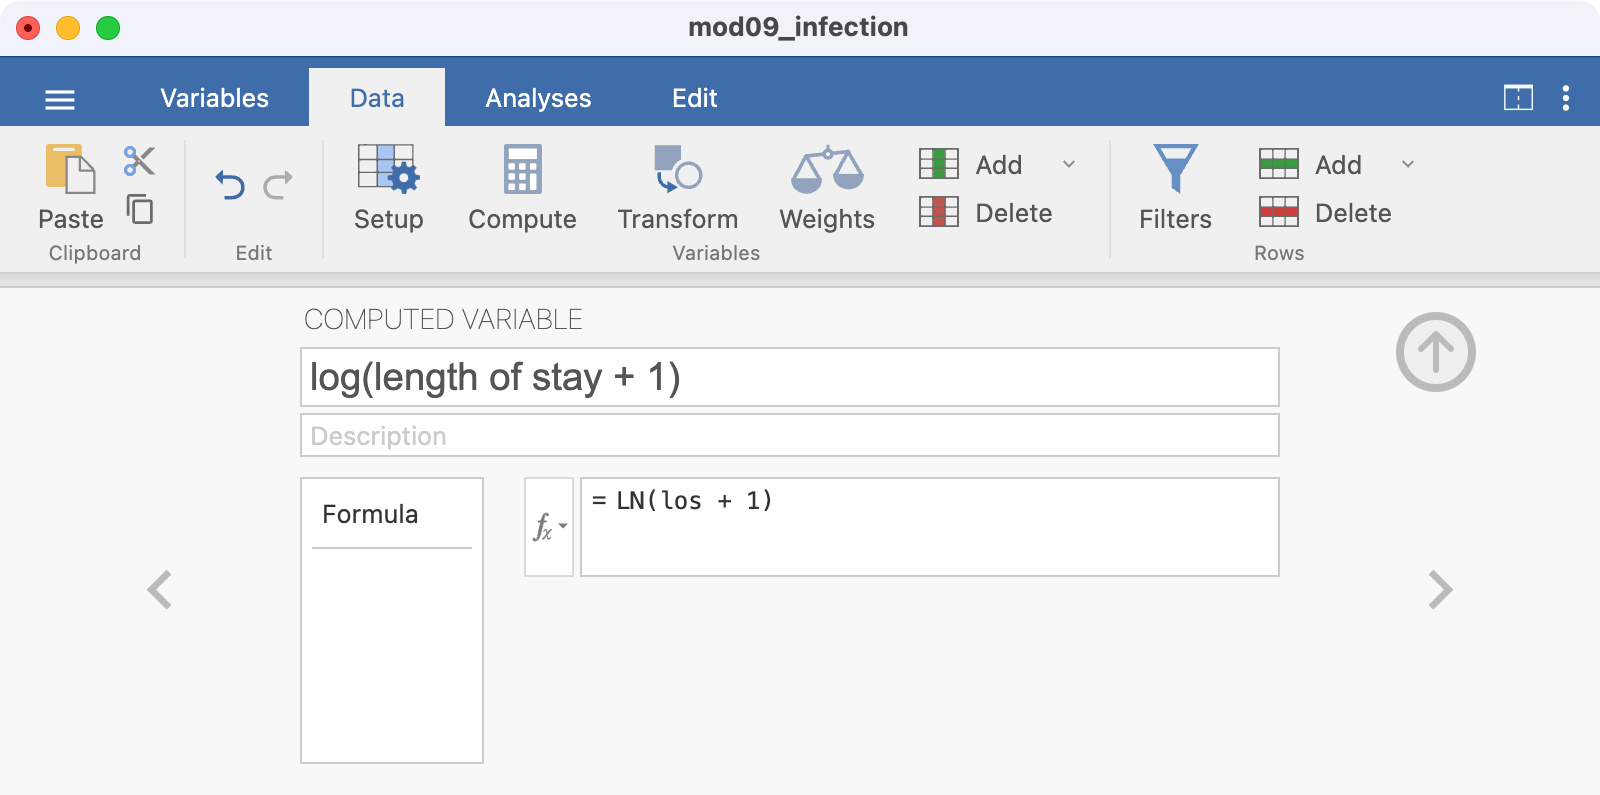
\includegraphics[keepaspectratio]{img/mod09/jamovi/mod09-gen1.png}}

You can now check whether this logged variable is normally distributed
as described in Module 2, for example by plotting a density plot as
shown in Figure 9.2.

To obtain the back-transformed mean, we can use a calculator to
calculate the exponential mean:

\(e^{3.407232} = 30.18\)

If your transformed variable is approximately normally distributed, you
can apply parametric tests such as the t-test. In the Worked Example 9.1
dataset, the variable \texttt{infect} (presence of nosocomial infection)
is a binary categorical variable. To test the hypothesis that patients
with nosocomial infection have a different length of stay to patients
without infection, you can conduct a t-test on the
\texttt{log(length\ of\ stay\ +\ 1)} variable. You will need to back
transform your mean values, as shown in Worked Example 9.1 in the course
notes when reporting your results.

\section{Wilcoxon ranked-sum test}\label{wilcoxon-ranked-sum-test}

The Wilcoxon ranked-sum test will be demonstrated using the length of
stay data in \texttt{mod09\_infection.rds}. Here, our continuous
variable is \texttt{los} and the grouping variable is \texttt{infect}.
Note that jamovi uses calls the Wilcoxon ranked-sum test the
\textbf{Mann-Whitney U} test. The two tests are equivalent.

The Wilcoxon ranked-sum test is conducted in \textbf{Analyses
\textgreater{} T-Tests \textgreater{} Independent Samples T-Test} in
jamovi. The screen is set up in the same way as for a two-sample t-test.
To conduct the Wilcoxon ranked-sum test, untick the \textbf{Student's}
box and click the \textbf{Mann-Whitney U} box in the \textbf{Tests}
section:

\pandocbounded{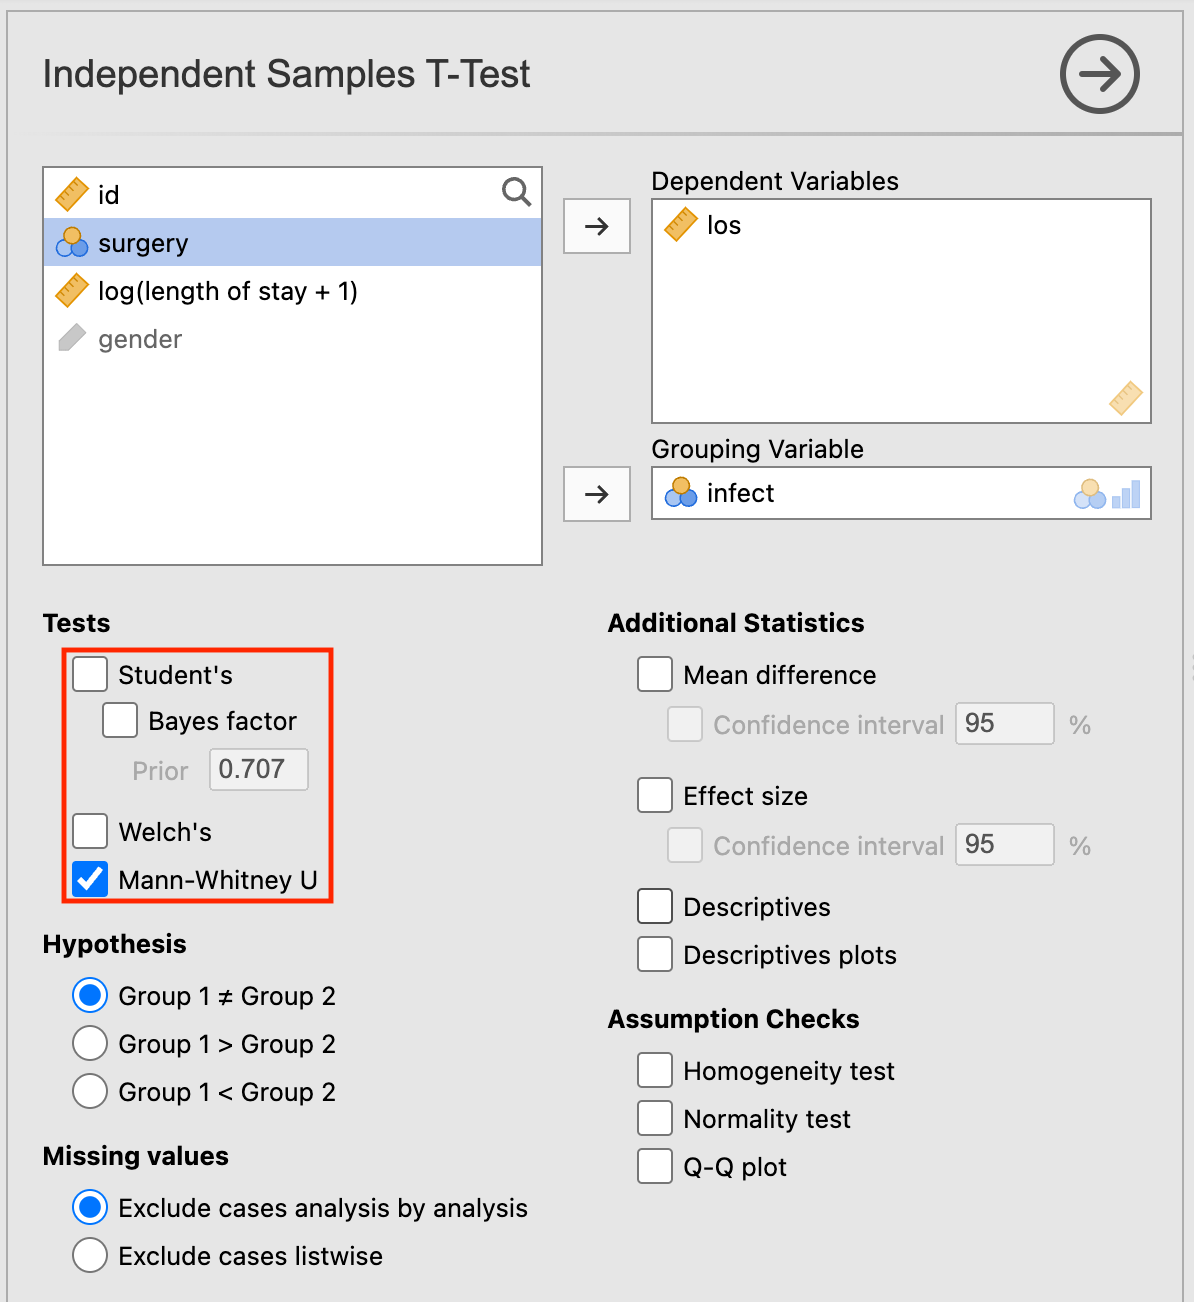
\includegraphics[keepaspectratio]{img/mod09/jamovi/mod09-wilcoxon.png}}

Note that the result appears without any descriptive analyses. You
should obtain the appropriate descriptive statistics in the usual way.

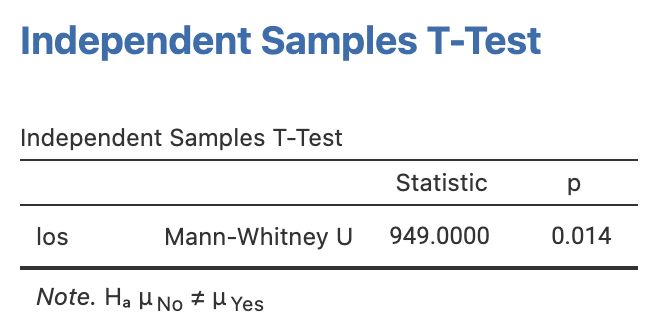
\includegraphics[width=0.5\linewidth,height=\textheight,keepaspectratio]{img/mod09/jamovi/mod09-wilcoxon-result.png}

\section{Wilcoxon matched-pairs signed-rank
test}\label{wilcoxon-matched-pairs-signed-rank-test}

The Wilcoxon ranked-sum test is conducted in jamovi using
\textbf{Analyses \textgreater{} T-Tests \textgreater{} Paired Samples
T-Test}.

We will demonstrate using the dataset on the arthritis drug cross-over
trial (\texttt{mod09\_arthritis.csv}). Like the paired t-test the paired
data need to be in separate columns.

\pandocbounded{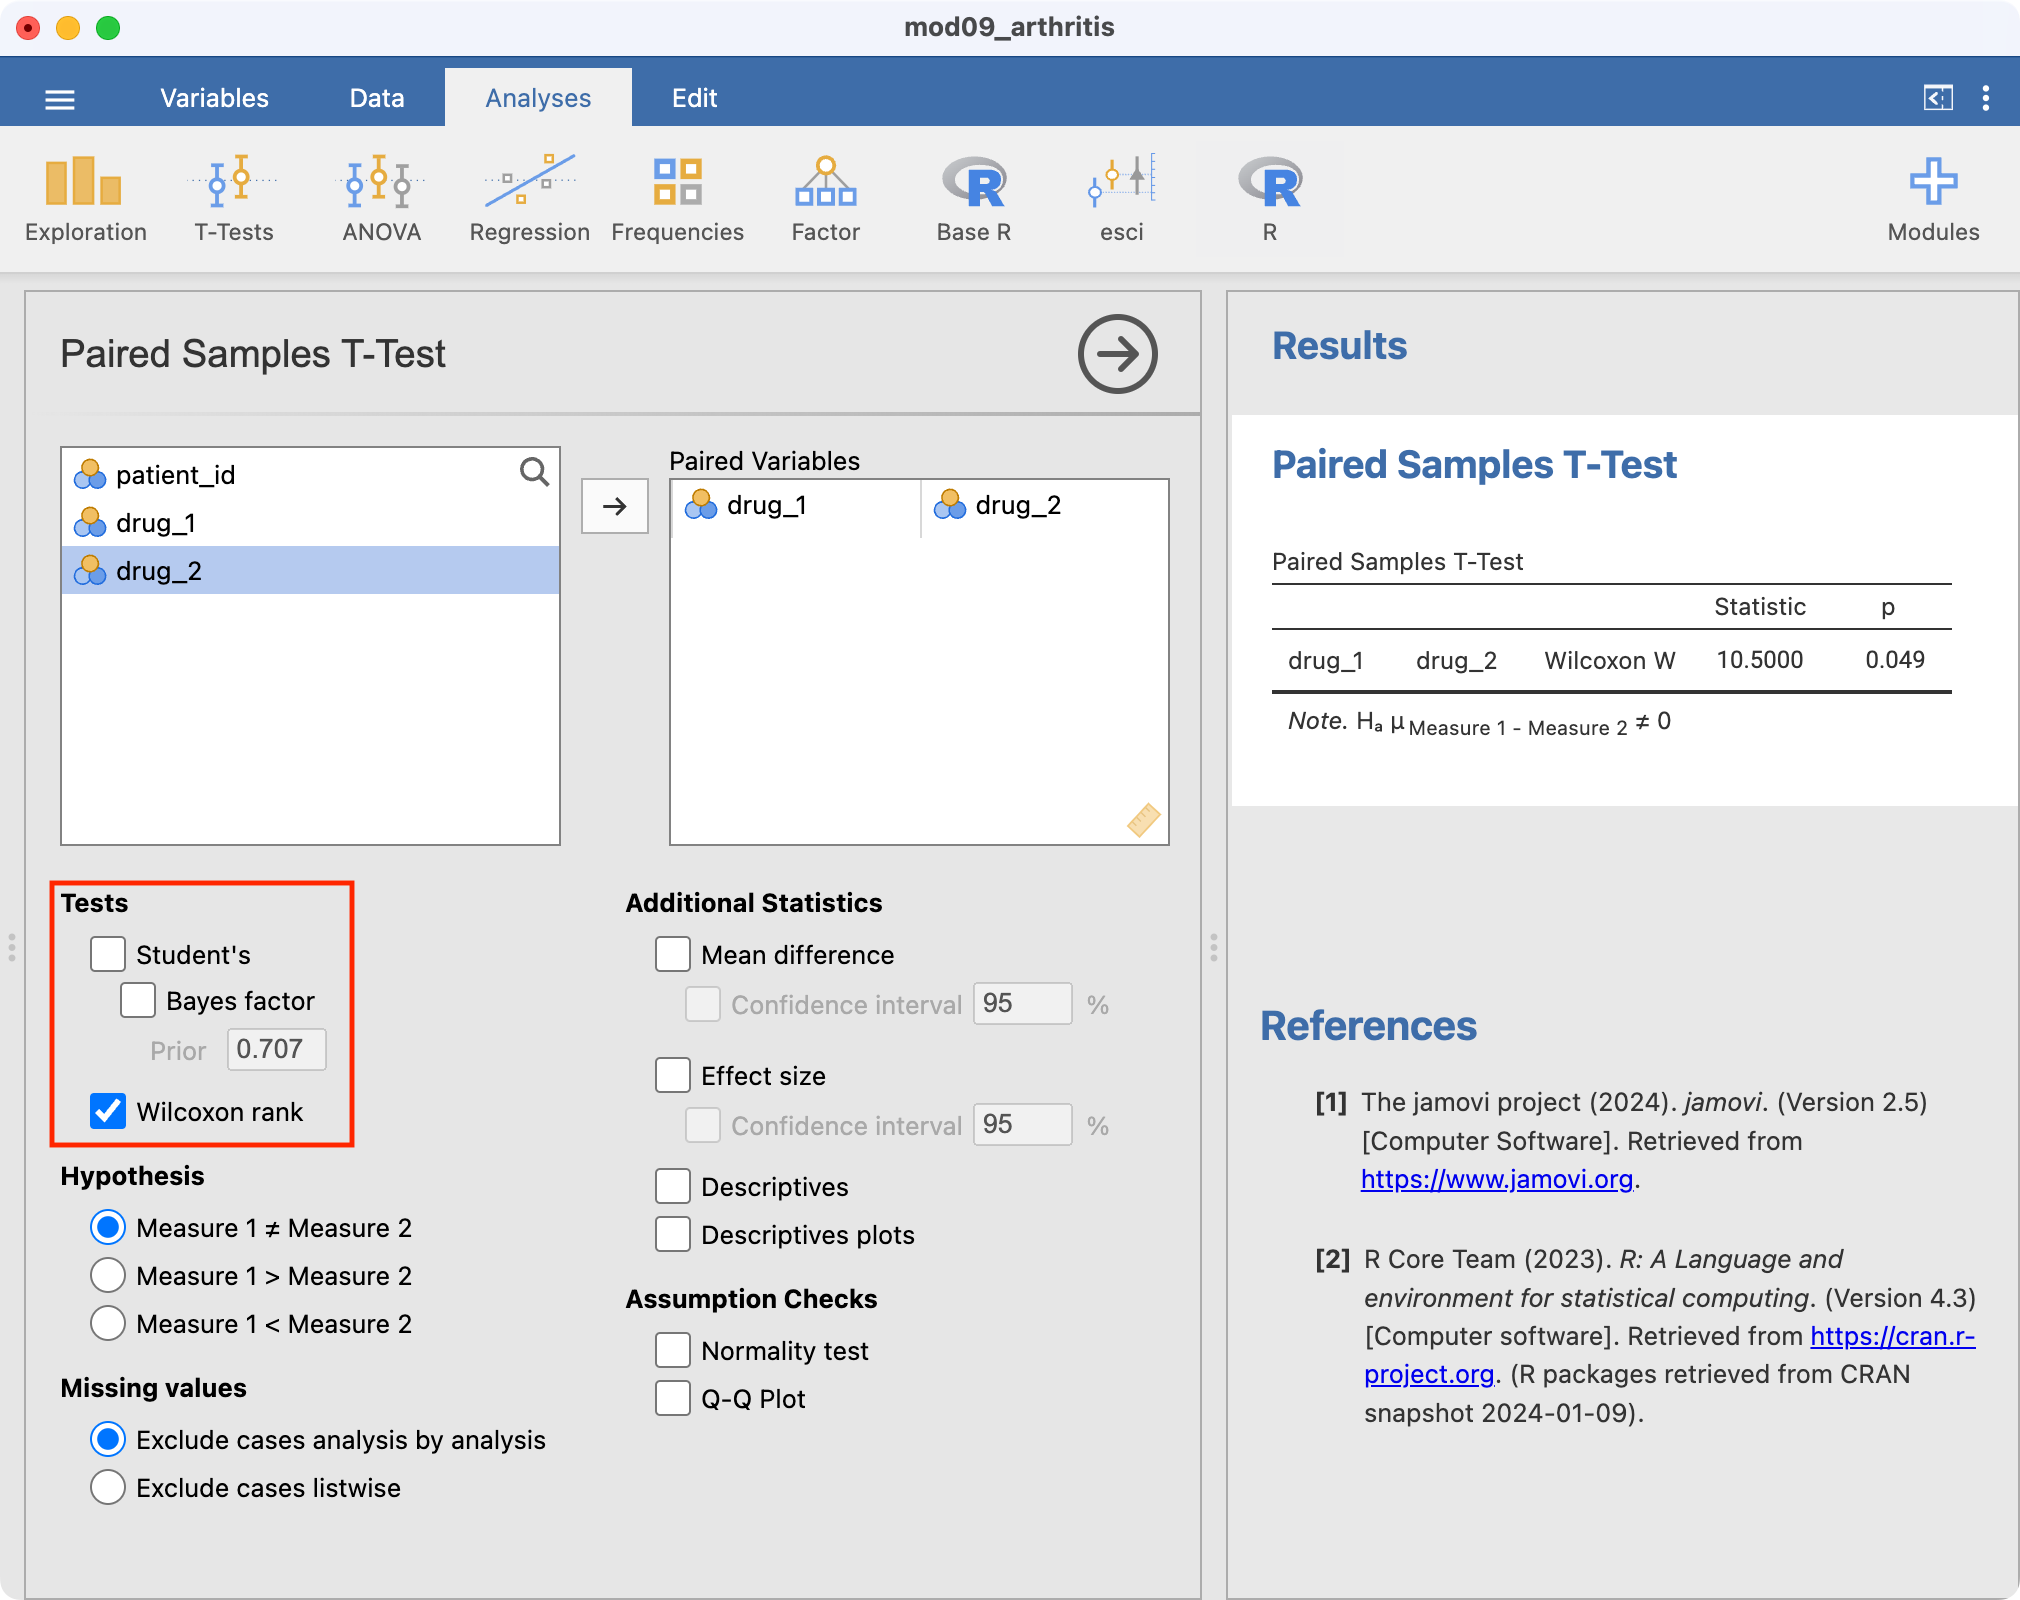
\includegraphics[keepaspectratio]{img/mod09/jamovi/mod09-wilcoxon-paired.png}}

\section{Estimating rank correlation
coefficients}\label{estimating-rank-correlation-coefficients}

The analyses for Spearman's and Kendall's rank correlation are conducted
in similar ways using \textbf{Regression \textgreater{} Correlation
Matrix}:

\pandocbounded{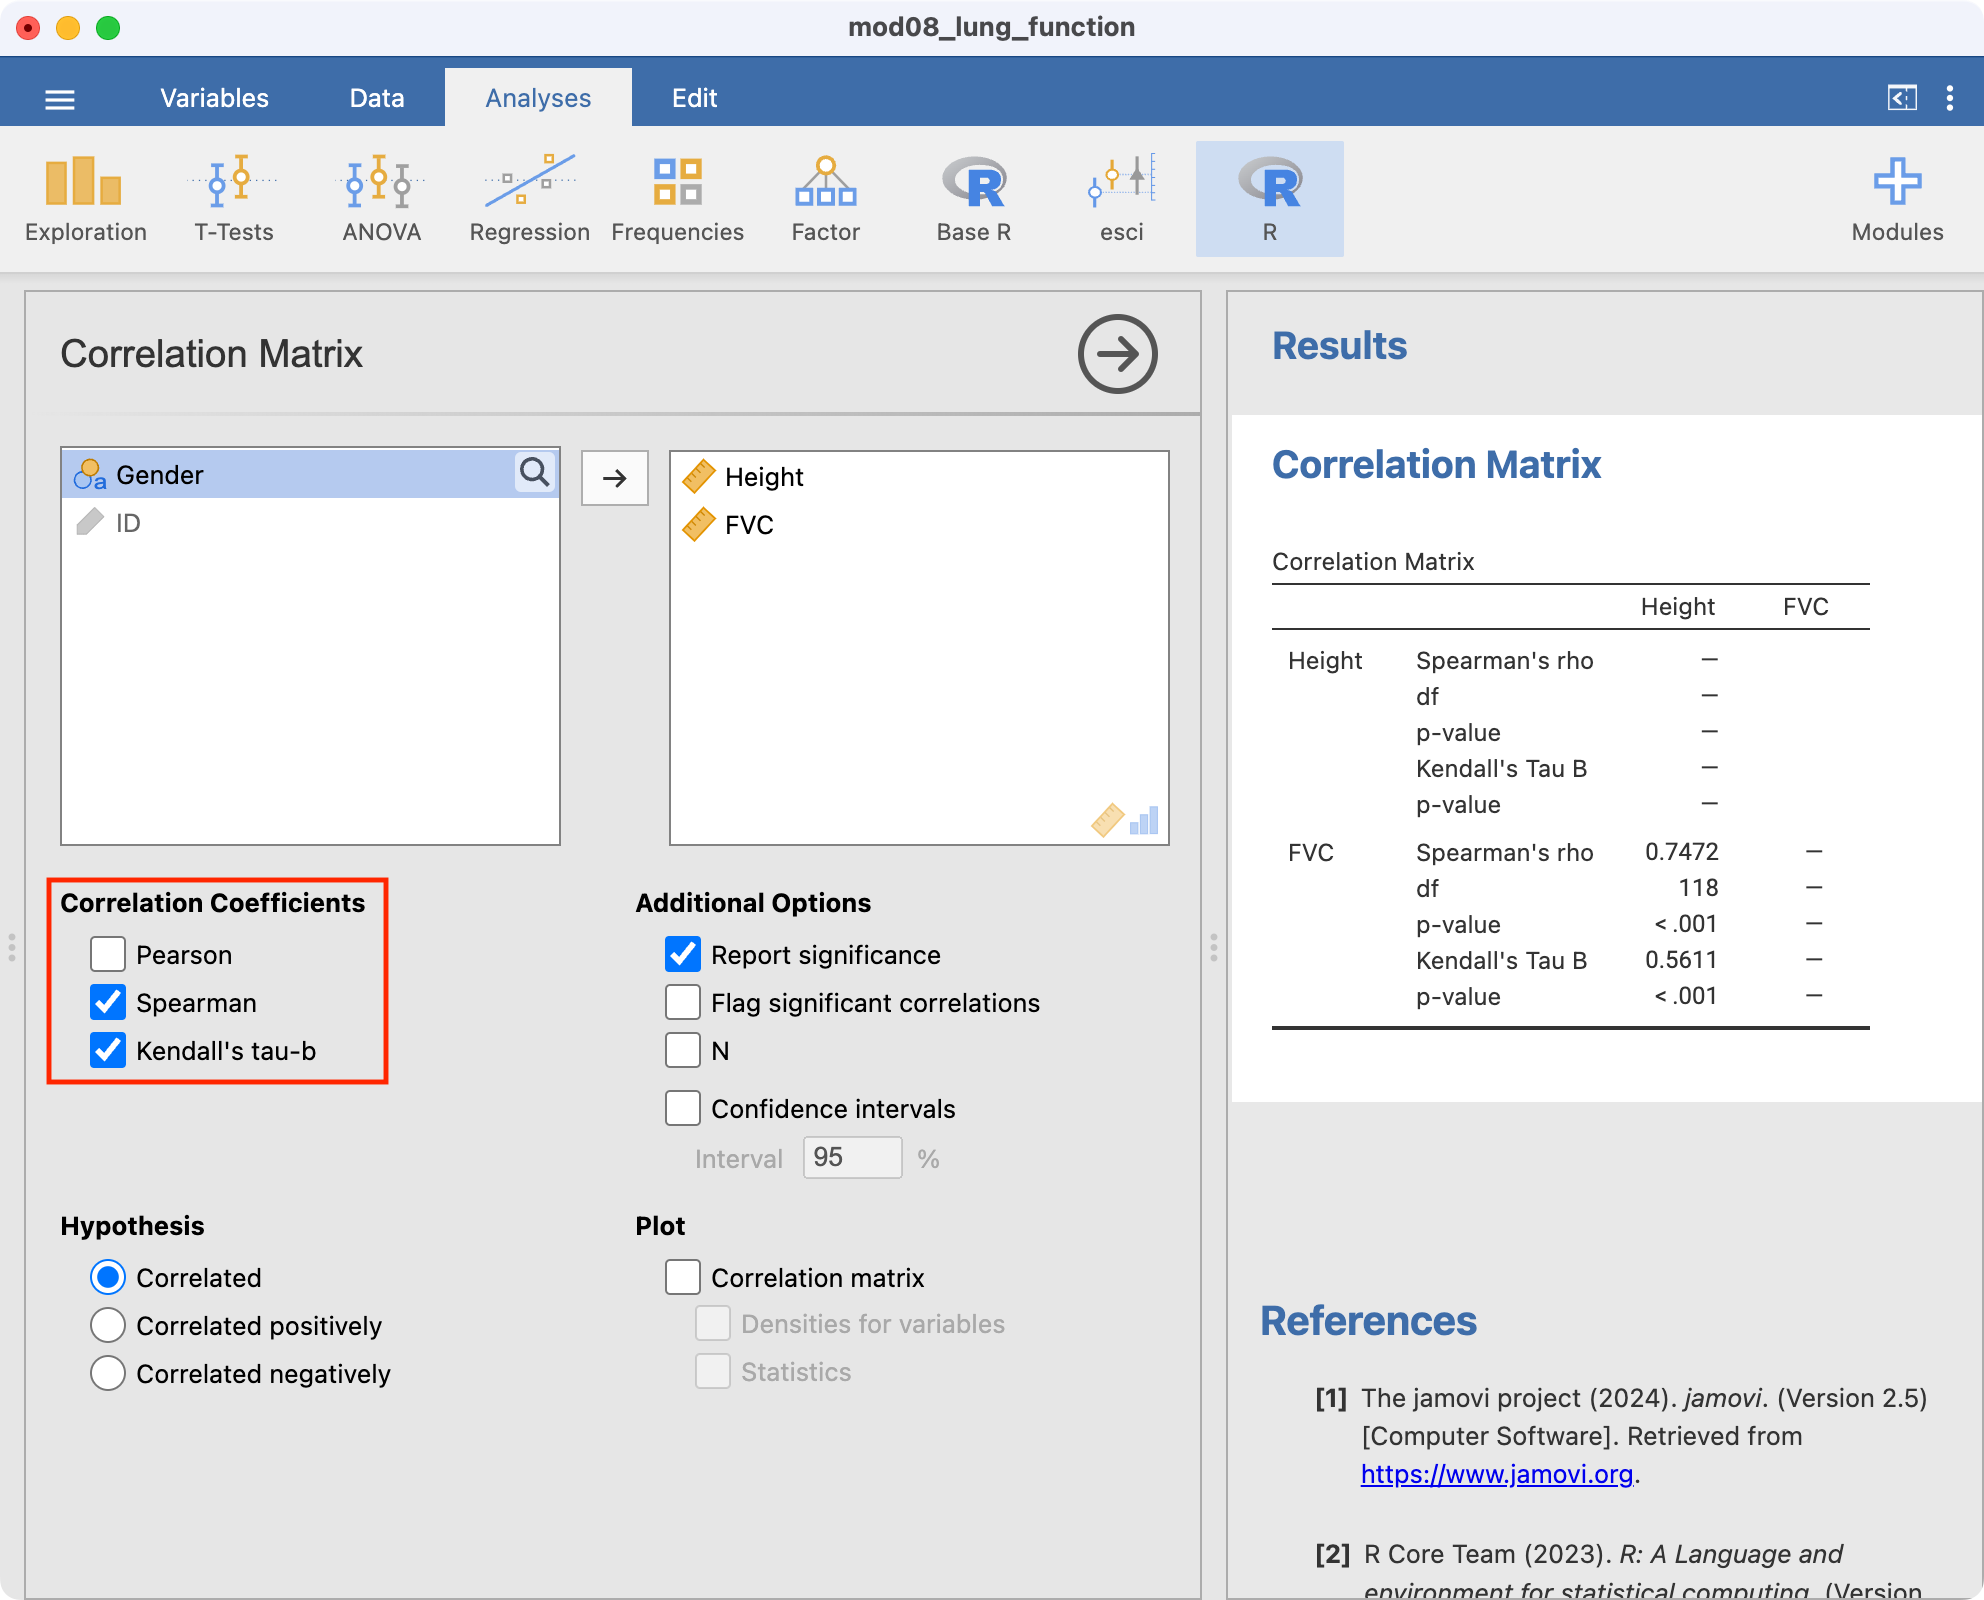
\includegraphics[keepaspectratio]{img/mod09/jamovi/mod09-corr.png}}

\newpage{}

\bookmarksetup{startatroot}

\chapter*{R notes}\label{r-notes-7}
\addcontentsline{toc}{chapter}{R notes}

\markboth{R notes}{R notes}

\section{Transforming non-normally distributed
variables}\label{transforming-non-normally-distributed-variables-2}

One option for dealing with a non-normally distributed varaible is to
transform it into its square, square root or logarithmic value. The new
transformed variable may be normally distributed and therefore a
parametric test can be used. First we check the distribution of the
variable for normality, e.g.~by plotting a histogram.

You can calculate a new, transformed, variable using standard commands.
For example, to create a new column of data based on the log of length
of stay:

\begin{Shaded}
\begin{Highlighting}[]
\FunctionTok{library}\NormalTok{(jmv)}
\FunctionTok{library}\NormalTok{(dplyr)}

\NormalTok{hospital }\OtherTok{\textless{}{-}} \FunctionTok{readRDS}\NormalTok{(}\StringTok{"data/examples/mod09\_infection.rds"}\NormalTok{) }\SpecialCharTok{|\textgreater{}} 
  \FunctionTok{mutate}\NormalTok{(}\AttributeTok{ln\_los =} \FunctionTok{log}\NormalTok{(los}\SpecialCharTok{+}\DecValTok{1}\NormalTok{))}

\FunctionTok{descriptives}\NormalTok{(}\AttributeTok{data=}\NormalTok{hospital, }\AttributeTok{vars=}\FunctionTok{c}\NormalTok{(los, ln\_los))}
\end{Highlighting}
\end{Shaded}

\begin{verbatim}

 DESCRIPTIVES

 Descriptives                                    
 ─────────────────────────────────────────────── 
                         los         ln_los      
 ─────────────────────────────────────────────── 
   N                          132          132   
   Missing                      0            0   
   Mean                  38.05303     3.407232   
   Median                27.00000     3.332205   
   Standard deviation    35.78057    0.7149892   
   Minimum               0.000000     0.000000   
   Maximum               244.0000     5.501258   
 ─────────────────────────────────────────────── 
\end{verbatim}

You can now check whether this logged variable is normally distributed
as described in Module 2, for example by plotting a histogram as shown
in Figure 9.2.

To obtain the back-transformed mean, we can use the \texttt{exp} command
to \texttt{anti-log} the mean:

\begin{Shaded}
\begin{Highlighting}[]
\FunctionTok{exp}\NormalTok{(}\FloatTok{3.407232}\NormalTok{)}
\end{Highlighting}
\end{Shaded}

\begin{verbatim}
[1] 30.18159
\end{verbatim}

If your transformed variable is approximately normally distributed, you
can apply parametric tests such as the t-test. In the Worked Example 9.1
dataset, the variable \texttt{infect} (presence of nosocomial infection)
is a binary categorical variable. To test the hypothesis that patients
with nosocomial infection have a different length of stay to patients
without infection, you can conduct a t-test on the \texttt{ln\_los}
variable. You will need to back transform your mean values, as shown in
Worked Example 9.1 in the course notes when reporting your results.

\section{Wilcoxon ranked-sum test}\label{wilcoxon-ranked-sum-test-1}

We use the \texttt{wilcox.test} function to perform the Wilcoxon
ranked-sum test:

\begin{verbatim}
wilcox.test(continuous_variable ~ group_variable, data=df)
\end{verbatim}

The Wilcoxon ranked-sum test will be demonstrated using the length of
stay data in \texttt{mod09\_infection.rds}. Here, out continuous
variable is \texttt{los} and the grouping variable is \texttt{infect}.

\begin{Shaded}
\begin{Highlighting}[]
\FunctionTok{wilcox.test}\NormalTok{(los }\SpecialCharTok{\textasciitilde{}}\NormalTok{ infect, }\AttributeTok{data=}\NormalTok{hospital)}
\end{Highlighting}
\end{Shaded}

\begin{verbatim}

    Wilcoxon rank sum test with continuity correction

data:  los by infect
W = 949, p-value = 0.01413
alternative hypothesis: true location shift is not equal to 0
\end{verbatim}

\section{Wilcoxon matched-pairs signed-rank
test}\label{wilcoxon-matched-pairs-signed-rank-test-1}

The \texttt{wilcox.test} function can also be used to conduct the
Wilcoxon matched-pairs signed-rank test. The specification of the
variables is a little different, in that each variable is specified as
\texttt{dataframe\$variable}:

\begin{verbatim}
wilcox.test(df$continuous_variable_1, df$continuous_variable_1, paired=TRUE)
\end{verbatim}

We will demonstrate using the dataset on the arthritis drug cross-over
trial (\texttt{mod09\_arthritis.csv}). Like the paired t-test the paired
data need to be in separate columns.

\begin{Shaded}
\begin{Highlighting}[]
\NormalTok{arthritis }\OtherTok{\textless{}{-}} \FunctionTok{read.csv}\NormalTok{(}\StringTok{"data/examples/mod09\_arthritis.csv"}\NormalTok{)}

\FunctionTok{wilcox.test}\NormalTok{(arthritis}\SpecialCharTok{$}\NormalTok{drug\_1, arthritis}\SpecialCharTok{$}\NormalTok{drug\_2, }
            \AttributeTok{paired=}\ConstantTok{TRUE}\NormalTok{)}
\end{Highlighting}
\end{Shaded}

\begin{verbatim}

    Wilcoxon signed rank exact test

data:  arthritis$drug_1 and arthritis$drug_2
V = 10.5, p-value = 0.0459
alternative hypothesis: true location shift is not equal to 0
\end{verbatim}

\section{Estimating rank correlation
coefficients}\label{estimating-rank-correlation-coefficients-1}

The analyses for Spearman's rank correlation is conducted similarly:

\begin{Shaded}
\begin{Highlighting}[]
\NormalTok{lung }\OtherTok{\textless{}{-}} \FunctionTok{read.csv}\NormalTok{(}\StringTok{"data/examples/mod08\_lung\_function.csv"}\NormalTok{)}

\FunctionTok{cor.test}\NormalTok{(lung}\SpecialCharTok{$}\NormalTok{Height, lung}\SpecialCharTok{$}\NormalTok{FVC, }\AttributeTok{method=}\StringTok{"spearman"}\NormalTok{)}
\end{Highlighting}
\end{Shaded}

\begin{verbatim}

    Spearman's rank correlation rho

data:  lung$Height and lung$FVC
S = 72796, p-value < 2.2e-16
alternative hypothesis: true rho is not equal to 0
sample estimates:
      rho 
0.7472186 
\end{verbatim}

\newpage{}

\bookmarksetup{startatroot}

\chapter*{Activities}\label{activities-8}
\addcontentsline{toc}{chapter}{Activities}

\markboth{Activities}{Activities}

\subsection*{Activity 9.1}\label{activity-9.1}
\addcontentsline{toc}{subsection}{Activity 9.1}

There is a hypothesis that university students who live and dine in the
university hall consume less vitamin C than the students who live and
dine at home. To test the hypothesis, 30 students were randomly selected
and their urinary ascorbic acid level was measured in mg over 3 hours.
Urinary excretion of ascorbic acid is a measure of vitamin C nutrition
in humans. The data is given in the following table and in the data set,
\texttt{Activity\_9.1.rds}.

\global\setlength{\Oldarrayrulewidth}{\arrayrulewidth}

\global\setlength{\Oldtabcolsep}{\tabcolsep}

\setlength{\tabcolsep}{2pt}

\renewcommand*{\arraystretch}{1.5}



\providecommand{\ascline}[3]{\noalign{\global\arrayrulewidth #1}\arrayrulecolor[HTML]{#2}\cline{#3}}

\begin{longtable*}[c]{|p{0.75in}|p{0.75in}}



\ascline{1.5pt}{666666}{1-2}

\multicolumn{1}{>{\centering}m{\dimexpr 0.75in+0\tabcolsep}}{\textcolor[HTML]{000000}{\fontsize{11}{11}\selectfont{\global\setmainfont{Helvetica}{Living\ and\ dining\ in\ Hall\ (n=17)}}}} & \multicolumn{1}{>{\centering}m{\dimexpr 0.75in+0\tabcolsep}}{\textcolor[HTML]{000000}{\fontsize{11}{11}\selectfont{\global\setmainfont{Helvetica}{Living\ and\ dining\ at\ Home\ (n\ =\ 13)}}}} \\

\ascline{1.5pt}{666666}{1-2}\endfirsthead 

\ascline{1.5pt}{666666}{1-2}

\multicolumn{1}{>{\centering}m{\dimexpr 0.75in+0\tabcolsep}}{\textcolor[HTML]{000000}{\fontsize{11}{11}\selectfont{\global\setmainfont{Helvetica}{Living\ and\ dining\ in\ Hall\ (n=17)}}}} & \multicolumn{1}{>{\centering}m{\dimexpr 0.75in+0\tabcolsep}}{\textcolor[HTML]{000000}{\fontsize{11}{11}\selectfont{\global\setmainfont{Helvetica}{Living\ and\ dining\ at\ Home\ (n\ =\ 13)}}}} \\

\ascline{1.5pt}{666666}{1-2}\endhead



\multicolumn{1}{>{\centering}m{\dimexpr 0.75in+0\tabcolsep}}{\textcolor[HTML]{000000}{\fontsize{11}{11}\selectfont{\global\setmainfont{Helvetica}{34}}}} & \multicolumn{1}{>{\centering}m{\dimexpr 0.75in+0\tabcolsep}}{\textcolor[HTML]{000000}{\fontsize{11}{11}\selectfont{\global\setmainfont{Helvetica}{163}}}} \\





\multicolumn{1}{>{\centering}m{\dimexpr 0.75in+0\tabcolsep}}{\textcolor[HTML]{000000}{\fontsize{11}{11}\selectfont{\global\setmainfont{Helvetica}{62}}}} & \multicolumn{1}{>{\centering}m{\dimexpr 0.75in+0\tabcolsep}}{\textcolor[HTML]{000000}{\fontsize{11}{11}\selectfont{\global\setmainfont{Helvetica}{205}}}} \\





\multicolumn{1}{>{\centering}m{\dimexpr 0.75in+0\tabcolsep}}{\textcolor[HTML]{000000}{\fontsize{11}{11}\selectfont{\global\setmainfont{Helvetica}{37}}}} & \multicolumn{1}{>{\centering}m{\dimexpr 0.75in+0\tabcolsep}}{\textcolor[HTML]{000000}{\fontsize{11}{11}\selectfont{\global\setmainfont{Helvetica}{83}}}} \\





\multicolumn{1}{>{\centering}m{\dimexpr 0.75in+0\tabcolsep}}{\textcolor[HTML]{000000}{\fontsize{11}{11}\selectfont{\global\setmainfont{Helvetica}{27}}}} & \multicolumn{1}{>{\centering}m{\dimexpr 0.75in+0\tabcolsep}}{\textcolor[HTML]{000000}{\fontsize{11}{11}\selectfont{\global\setmainfont{Helvetica}{372}}}} \\





\multicolumn{1}{>{\centering}m{\dimexpr 0.75in+0\tabcolsep}}{\textcolor[HTML]{000000}{\fontsize{11}{11}\selectfont{\global\setmainfont{Helvetica}{38}}}} & \multicolumn{1}{>{\centering}m{\dimexpr 0.75in+0\tabcolsep}}{\textcolor[HTML]{000000}{\fontsize{11}{11}\selectfont{\global\setmainfont{Helvetica}{50}}}} \\





\multicolumn{1}{>{\centering}m{\dimexpr 0.75in+0\tabcolsep}}{\textcolor[HTML]{000000}{\fontsize{11}{11}\selectfont{\global\setmainfont{Helvetica}{20}}}} & \multicolumn{1}{>{\centering}m{\dimexpr 0.75in+0\tabcolsep}}{\textcolor[HTML]{000000}{\fontsize{11}{11}\selectfont{\global\setmainfont{Helvetica}{22}}}} \\





\multicolumn{1}{>{\centering}m{\dimexpr 0.75in+0\tabcolsep}}{\textcolor[HTML]{000000}{\fontsize{11}{11}\selectfont{\global\setmainfont{Helvetica}{7}}}} & \multicolumn{1}{>{\centering}m{\dimexpr 0.75in+0\tabcolsep}}{\textcolor[HTML]{000000}{\fontsize{11}{11}\selectfont{\global\setmainfont{Helvetica}{47}}}} \\





\multicolumn{1}{>{\centering}m{\dimexpr 0.75in+0\tabcolsep}}{\textcolor[HTML]{000000}{\fontsize{11}{11}\selectfont{\global\setmainfont{Helvetica}{53}}}} & \multicolumn{1}{>{\centering}m{\dimexpr 0.75in+0\tabcolsep}}{\textcolor[HTML]{000000}{\fontsize{11}{11}\selectfont{\global\setmainfont{Helvetica}{255}}}} \\





\multicolumn{1}{>{\centering}m{\dimexpr 0.75in+0\tabcolsep}}{\textcolor[HTML]{000000}{\fontsize{11}{11}\selectfont{\global\setmainfont{Helvetica}{22}}}} & \multicolumn{1}{>{\centering}m{\dimexpr 0.75in+0\tabcolsep}}{\textcolor[HTML]{000000}{\fontsize{11}{11}\selectfont{\global\setmainfont{Helvetica}{30}}}} \\





\multicolumn{1}{>{\centering}m{\dimexpr 0.75in+0\tabcolsep}}{\textcolor[HTML]{000000}{\fontsize{11}{11}\selectfont{\global\setmainfont{Helvetica}{37}}}} & \multicolumn{1}{>{\centering}m{\dimexpr 0.75in+0\tabcolsep}}{\textcolor[HTML]{000000}{\fontsize{11}{11}\selectfont{\global\setmainfont{Helvetica}{89}}}} \\





\multicolumn{1}{>{\centering}m{\dimexpr 0.75in+0\tabcolsep}}{\textcolor[HTML]{000000}{\fontsize{11}{11}\selectfont{\global\setmainfont{Helvetica}{14}}}} & \multicolumn{1}{>{\centering}m{\dimexpr 0.75in+0\tabcolsep}}{\textcolor[HTML]{000000}{\fontsize{11}{11}\selectfont{\global\setmainfont{Helvetica}{96}}}} \\





\multicolumn{1}{>{\centering}m{\dimexpr 0.75in+0\tabcolsep}}{\textcolor[HTML]{000000}{\fontsize{11}{11}\selectfont{\global\setmainfont{Helvetica}{28}}}} & \multicolumn{1}{>{\centering}m{\dimexpr 0.75in+0\tabcolsep}}{\textcolor[HTML]{000000}{\fontsize{11}{11}\selectfont{\global\setmainfont{Helvetica}{48}}}} \\





\multicolumn{1}{>{\centering}m{\dimexpr 0.75in+0\tabcolsep}}{\textcolor[HTML]{000000}{\fontsize{11}{11}\selectfont{\global\setmainfont{Helvetica}{28}}}} & \multicolumn{1}{>{\centering}m{\dimexpr 0.75in+0\tabcolsep}}{\textcolor[HTML]{000000}{\fontsize{11}{11}\selectfont{\global\setmainfont{Helvetica}{25}}}} \\





\multicolumn{1}{>{\centering}m{\dimexpr 0.75in+0\tabcolsep}}{\textcolor[HTML]{000000}{\fontsize{11}{11}\selectfont{\global\setmainfont{Helvetica}{70}}}} & \multicolumn{1}{>{\centering}m{\dimexpr 0.75in+0\tabcolsep}}{\textcolor[HTML]{000000}{\fontsize{11}{11}\selectfont{\global\setmainfont{Helvetica}{163}}}} \\





\multicolumn{1}{>{\centering}m{\dimexpr 0.75in+0\tabcolsep}}{\textcolor[HTML]{000000}{\fontsize{11}{11}\selectfont{\global\setmainfont{Helvetica}{16}}}} & \multicolumn{1}{>{\centering}m{\dimexpr 0.75in+0\tabcolsep}}{\textcolor[HTML]{000000}{\fontsize{11}{11}\selectfont{\global\setmainfont{Helvetica}{}}}} \\





\multicolumn{1}{>{\centering}m{\dimexpr 0.75in+0\tabcolsep}}{\textcolor[HTML]{000000}{\fontsize{11}{11}\selectfont{\global\setmainfont{Helvetica}{9}}}} & \multicolumn{1}{>{\centering}m{\dimexpr 0.75in+0\tabcolsep}}{\textcolor[HTML]{000000}{\fontsize{11}{11}\selectfont{\global\setmainfont{Helvetica}{}}}} \\





\multicolumn{1}{>{\centering}m{\dimexpr 0.75in+0\tabcolsep}}{\textcolor[HTML]{000000}{\fontsize{11}{11}\selectfont{\global\setmainfont{Helvetica}{121}}}} & \multicolumn{1}{>{\centering}m{\dimexpr 0.75in+0\tabcolsep}}{\textcolor[HTML]{000000}{\fontsize{11}{11}\selectfont{\global\setmainfont{Helvetica}{}}}} \\

\ascline{1.5pt}{666666}{1-2}



\end{longtable*}



\arrayrulecolor[HTML]{000000}

\global\setlength{\arrayrulewidth}{\Oldarrayrulewidth}

\global\setlength{\tabcolsep}{\Oldtabcolsep}

\renewcommand*{\arraystretch}{1}

Analyse these data to assess the research question.

\subsection*{Activity 9.2}\label{activity-9.2}
\addcontentsline{toc}{subsection}{Activity 9.2}

Researchers conducted a study to assess the effect of a health promotion
campaign in increasing dietary fibre intake. Participants completed a
food diary before and after the campaign, from which daily fibre intake
(measured in grams) was estimated.

The dataset \texttt{Activity\_9.2.csv} contains the following variables:

\begin{itemize}
\tightlist
\item
  id: participant ID number
\item
  gender: participant gender (1=male, 2=female)
\item
  age\_yrs: participant age (years)
\item
  fibre\_pre: daily fibre consumption before the campaign (grams)
\item
  fibre\_post: daily fibre consumption after the campaign (grams)
\end{itemize}

Analyse these data to answer the research question.

\subsection*{Activity 9.3}\label{activity-9.3}
\addcontentsline{toc}{subsection}{Activity 9.3}

It is often necessary to take blood from newborn babies, which causes
them pain. A group of researchers wanted to test whether a pacifier
(dummy) would provide some pain relief. Newborn babies undergoing
venepuncture were randomised to one of two treatment groups. In the
placebo group, babies had blood taken as per the usual protocol. In the
pacifier group, babies were allowed to suck on a pacifier while having
their blood taken. Each venepuncture was observed by an assessor, who
rated the baby's pain on the DAN scale which ranges from 0 (no pain) to
10. The DAN is based on observation of the baby's facial expression,
limb movement, and vocal expression. The data are provided in the file
\texttt{Activity\_9.3.csv}.

Analyse these data to answer the research question.

\subsection*{Supplementary Activity
9.4}\label{supplementary-activity-9.4}
\addcontentsline{toc}{subsection}{Supplementary Activity 9.4}

A study was conducted among 201 people who had recently quit smoking.
The dataset \texttt{Activity\_9.4\_smoke.csv} contains the following
variables:

\begin{itemize}
\tightlist
\item
  ID: participant ID number
\item
  age: participant age (years)
\item
  gender: participant gender (1=Male, 2=Female)
\item
  day\_abs: number of days abstinent (i.e., number of days since last
  cigarette)
\end{itemize}

Analyse these data to assess whether there is a difference in the number
of days abstinent between males and females.

\bookmarksetup{startatroot}

\chapter{An introduction to sample size
estimation}\label{an-introduction-to-sample-size-estimation}

\section*{Learning objectives}\label{learning-objectives-9}
\addcontentsline{toc}{section}{Learning objectives}

\markright{Learning objectives}

By the end of this module you will be able to:

\begin{itemize}
\tightlist
\item
  Explain the issues involved in sample size estimation for
  epidemiological studies;
\item
  Estimate sample sizes for descriptive and analytic studies;
\item
  Compute the sample size needed for planned statistical tests;
\item
  Adjust sample size calculations for factors that influence study
  power.
\end{itemize}

\section*{Optional readings}\label{optional-readings-9}
\addcontentsline{toc}{section}{Optional readings}

\markright{Optional readings}

Kirkwood and Sterne (2001); Chapter 35.
\href{http://er1.library.unsw.edu.au/er/cgi-bin/eraccess.cgi?url=https://ebookcentral.proquest.com/lib/unsw/detail.action?docID=624728}{{[}UNSW
Library Link{]}}

Bland (2015); Chapter 18.
\href{http://er1.library.unsw.edu.au/er/cgi-bin/eraccess.cgi?url=https://ebookcentral.proquest.com/lib/unsw/detail.action?docID=5891730}{{[}UNSW
Library Link{]}}

For interest: Woodward (2013); Chapter 8.
\href{http://er1.library.unsw.edu.au/er/cgi-bin/eraccess.cgi?url=https://ebookcentral.proquest.com/lib/unsw/detail.action?docID=1575748}{{[}UNSW
Library Link{]}}

\section{Introduction}\label{introduction-9}

Determining the appropriate sample size (the number of participants in a
study) is one of the most critical issues when designing a research
study. A common question when planning a project is ``How many
participants do I need?'' The sample size needs to be large enough to
ensure that the results can be generalised to the population and will be
accurate, but small enough for the study question to be answered with
the resources available. In general, the larger the sample size, the
more precise the study results will be.

Unfortunately, estimating the sample size required for a study is not
straightforward and the method used varies with the study design and the
type of statistical test that will be conducted on the data collected.
In the past, researchers calculated the sample size by hand using
complicated mathematical formula. More recently, look-up tables have
been created which has removed the need for hand calculations. Now, most
researchers use computer programs where parameters relevant to the
particular study design are entered and the sample size is automatically
calculated. In this module, we will use an abbreviated look-up table to
demonstrate the parameters that need to be considered when estimating
sample sizes for a confidence interval and use software for all other
sample size calculations. The look-up table allows you to see at a
glance, the impact of different factors on the sample size estimation.

\subsection{Under and over-sized
studies}\label{under-and-over-sized-studies}

In health research, there are different implications for interpreting
the results if the sample size is too small or too large.

An under-sized study is one which lacks the power to find an effect or
association when, in truth, one exists. If the sample size is too small,
an important difference between groups may not be statistically
significant and so will not be detected by the study. In fact, it is
considered unethical to conduct a health study which is poorly designed
so that it is not possible to detect an effect or association if it
exists. Often, Ethics Committees request evidence of sample size
calculations before a study is approved.

A classic paper by Freiman et al examined 71 randomised controlled
trials which reported an absence of clinical effect between two
treatments.(Freiman et al. 1978) Many of the trials were too small to
show that a clinically important difference was statistically
significant. If the sample size of an analytic study is too small, then
only very limited conclusions can be drawn about the results.

In general, the larger the sample size the more precise the estimates
will be. However, large sample sizes have their own effect on the
interpretation of the results. An over-sized study is one in which a
small difference between groups, which is not important in clinical or
public health terms, is statistically significant. When the study sample
is large, the null hypothesis could be rejected in error and research
resources may be wasted. This type of study may be unethical due to the
unnecessary enrolment of a large number of people.

\section{Sample size estimation for descriptive
studies}\label{sample-size-estimation-for-descriptive-studies}

To estimate the sample size required for a descriptive study, we usually
focus on specifying the width of the confidence interval around our
primary estimate. For example, to estimate the sample size for a study
designed to measure a prevalence we need to:

\begin{itemize}
\tightlist
\item
  nominate the expected prevalence based on other available evidence;
\item
  nominate the required level of precision around the estimate. For
  this, the width of the 95\% confidence interval (i.e.~the distance
  equal to 1.96 \(\times\) SE) is used.
\end{itemize}

Table~\ref{tbl-10-1} is an abbreviated look-up table that we can use to
estimate the sample size for this type of study. Note that the sample
size required to detect an expected population prevalence of 5\% is the
same as to detect a prevalence of 95\%. Similarly 10\% is equivalent to
90\% etc. It is symmetric about 50\%. From Table~\ref{tbl-10-1}, you can
see that the sample size required increases as the expected prevalence
approaches 50\% and as the precision increases (i.e.~the required 95\%
CI becomes narrower).

\begin{table}[h]

\caption{\label{tbl-10-1}Sample size required to calculate a 95\%
confidence interval with a given precision}

\centering{

\centering
\begin{tblr}[         %% tabularray outer open
]                     %% tabularray outer close
{                     %% tabularray inner open
colspec={Q[]Q[]Q[]Q[]Q[]Q[]Q[]Q[]Q[]Q[]Q[]},
hline{2}={3-11}{solid, black, 0.03em},
hline{2}={2}{solid, black, 0.03em, l=-0.5},
hline{3}={1-11}{solid, black, 0.05em},
hline{1}={1-11}{solid, black, 0.08em},
hline{8}={1-11}{solid, black, 0.08em},
column{1,3-11}={}{halign=c},
row{2,3,4,5,6,7}={}{halign=c},
cell{1}{2}={c=10}{halign=c},
}                     %% tabularray inner close
& Required confidence interval width &  &  &  &  &  &  &  &  &  \\
Prevalence of outcome & 1\% & 1.5\% & 2\% & 2.5\% & 3\% & 3.5\% & 4\% & 5\% & 10\% & 15\% \\
5\% or 95\% & 1825 & 812 & 457 & 292 & 203 & 149 & 115 &   &   &   \\
10\% or 90\% & 3458 & 1537 & 865 & 554 & 385 & 283 & 217 & 139 &   &   \\
15\% or 85\% & 4899 & 2177 & 1225 & 784 & 545 & 400 & 307 & 196 & 49 &   \\
20\% or 80\% & 6147 & 2732 & 1537 & 984 & 683 & 502 & 385 & 246 & 62 & 28 \\
25\% or 75\% & 7203 & 3202 & 1801 & 1153 & 801 & 588 & 451 & 289 & 73 & 33 \\
\end{tblr}

}

\end{table}%

\subsection{Worked Example 10.1}\label{wex10-1}

A descriptive cross-sectional study is designed to measure the
prevalence of bronchitis in children age 0-2 years with a 95\% CI of
\(\pm\) 4\%. The prevalence is expected to be 20\%. From the table, a
sample size of at least 385 will be required for the width of the 95\%
CI to be \(\pm\) 4\% (i.e.~the reported precision of the summary
statistic will be 20\% (95\% CI 16\% to 24\%)).

If the prevalence turns out to be higher than the researchers expected
or if they decided that they wanted a narrower 95\% CI (i.e.~increase
precision), a larger sample size would be required.

\begin{itemize}
\tightlist
\item
  What sample size would be required if the prevalence was 15\% and the
  desired 95\% CI was \(\pm\) 3\%?
\item
  Answer: 545
\end{itemize}

\section{Sample size estimation for analytic
studies}\label{sample-size-estimation-for-analytic-studies}

Analytic study designs are used to compare characteristics between
different groups in the population. The main study designs are analytic
cross-sectional studies, case-control studies, cohort studies and
randomised controlled trials. For analytic study designs, the outcome
measure of interest can be a mean value, a proportion or a relative risk
if a random sample has been enrolled. For case-control studies the most
appropriate measure of association is an odds ratio.

\subsection{Factors to be considered}\label{factors-to-be-considered}

The first important decision in estimating a required sample size for an
analytic study is to select the type of statistical test that will be
used to report or analyse the data. Each type of test is associated with
a different method of sample size estimation.

Once the statistical method has been determined, the following issues
need to be decided:

\begin{itemize}
\tightlist
\item
  Statistical power: the chance of finding a difference if one exists,
  e.g.~80\%;
\item
  Level of significance: the P value that will be considered
  significant, e.g.~P\textless0.05;
\item
  Minimum effect size of interest: the size of the difference between
  groups e.g.~the difference in the proportion of parents who oppose
  immunisation in two different regions or the difference in mean values
  of blood pressure in two groups of people with different types of
  cardiac disease;
\item
  Variability: the spread of the measurements, e.g.~the expected
  standard deviation of the main outcome variable (if continuous), or
  the expected proportions;
\item
  Resources: an estimate of the number of participants available and
  amount of funding to run the study.
\end{itemize}

In addition to deciding the level of power and probability that will be
used, the difference between groups that is regarded as being important
has to be estimated. The smallest difference between study groups that
we want to detect is described as the minimum expected effect size. This
is determined on the basis of clinical judgement, public health
importance and expertise in the condition being researched, or may it be
need to be determined from a pilot study or a literature review. The
smaller the expected effect or association, the larger the sample size
will need to obtain statistical significance. We also need some
knowledge of how variable the measurement is expected to be. For this we
often use the standard deviation for a continuous measure. As
measurement variability increases, the sample size will need to increase
in order to detect the expected difference between the groups. Above
all, a study has to be practical in terms of the availability of a
population from which to draw sufficient numbers for the study and in
terms of the funds that are available to conduct the study.

\newpage

\subsection{Power and significance
level}\label{power-and-significance-level}

The power of a study, which was discussed in Module 4, is the chance of
finding a statistically significant difference when one exists, i.e.~the
probability of correctly rejecting the null hypothesis. The relationship
between the power of a study and statistical significance is shown in
Table~\ref{tbl-truth-vs-study-html}.

\begin{longtable}[]{@{}
  >{\raggedright\arraybackslash}p{(\linewidth - 4\tabcolsep) * \real{0.3000}}
  >{\centering\arraybackslash}p{(\linewidth - 4\tabcolsep) * \real{0.4111}}
  >{\centering\arraybackslash}p{(\linewidth - 4\tabcolsep) * \real{0.2889}}@{}}
\caption{Comparison of study result with the
truth}\label{tbl-truth-vs-study-html}\tabularnewline
\toprule\noalign{}
\begin{minipage}[b]{\linewidth}\raggedright
\end{minipage} & \begin{minipage}[b]{\linewidth}\centering
\textbf{Effect in reality}
\end{minipage} & \begin{minipage}[b]{\linewidth}\centering
\textbf{No effect in reality}
\end{minipage} \\
\midrule\noalign{}
\endfirsthead
\toprule\noalign{}
\begin{minipage}[b]{\linewidth}\raggedright
\end{minipage} & \begin{minipage}[b]{\linewidth}\centering
\textbf{Effect in reality}
\end{minipage} & \begin{minipage}[b]{\linewidth}\centering
\textbf{No effect in reality}
\end{minipage} \\
\midrule\noalign{}
\endhead
\bottomrule\noalign{}
\endlastfoot
\textbf{Evidence was found} & Correct: Power (\(1 - \beta\)) & Error:
\(\alpha\) \\
\textbf{No evidence was found} & Error: \(\beta\) & Correct \\
\end{longtable}

The power of a study is expressed as 1 - β where β is the probability of
a false negative (that is, the probability of a Type II error -
incorrectly not rejecting the null hypothesis. In most research, power
is generally set to 80\% (a Type II error rate of 20\%). However, in
some studies, especially in some clinical trials where rigorous results
are required, power is set to 90\% (a Type II error rate of 10\%).

The significance level, or α level, is the level at which the P value of
a test is considered to be statistically significant. The α level is
usually set at 5\% indicating a probability of \textless0.05 will be
regarded as statistically significant. Occasionally, especially if
several outcome measures are being compared, the α level is set at 1\%
indicating a probability of \textless0.01 will be regarded as
statistically significant.

The calculation of sample sizes for analytic studies are based on
calculations that are somewhat tedious to compute by hand. Software
packages or online sample size calculators are the standard method of
calculating sample sizes for analytic studies. In this module, we will
demonstrate the use of an online calculator called PS, available at
https://cqsclinical.app.vumc.org/ps/

\section{Detecting the difference between two
means}\label{detecting-the-difference-between-two-means}

The test that is used to show that two mean values are significantly
different from one another is the independent samples t-test (Module 5).
The sample size needed for this test to have sufficient power can be
calculated using PS as shown in the Worked Example below.

\subsection{Worked Example 10.2}\label{worked-example-10.2}

There is a hypothesis that the use of the oral contraceptive (OC) pill
in premenopausal women can increase systolic blood pressure. A study was
planned to test this hypothesis using a two sided t-test. The
investigators are interested in detecting an increase of at least 5 mm
Hg systolic blood pressure in the women using OC compared to the non-OC
users with 90\% power at a 5\% significance level. A pilot study shows
that the SD of systolic blood pressure in the target group is 25 mm Hg
and the mean systolic blood pressure of non-OC user women is 110 mm Hg.
What is the minimum number of women in each group that need to be
recruited for the study to detect this difference?

\textbf{Solution} The effect size of interest is 5 mm Hg and the
associated standard deviation is 25 mm Hg. For power of 90\% and alpha
of 5\%, the sample size calculation using the \textbf{t-test
\textgreater{} Independent} tab of PS:

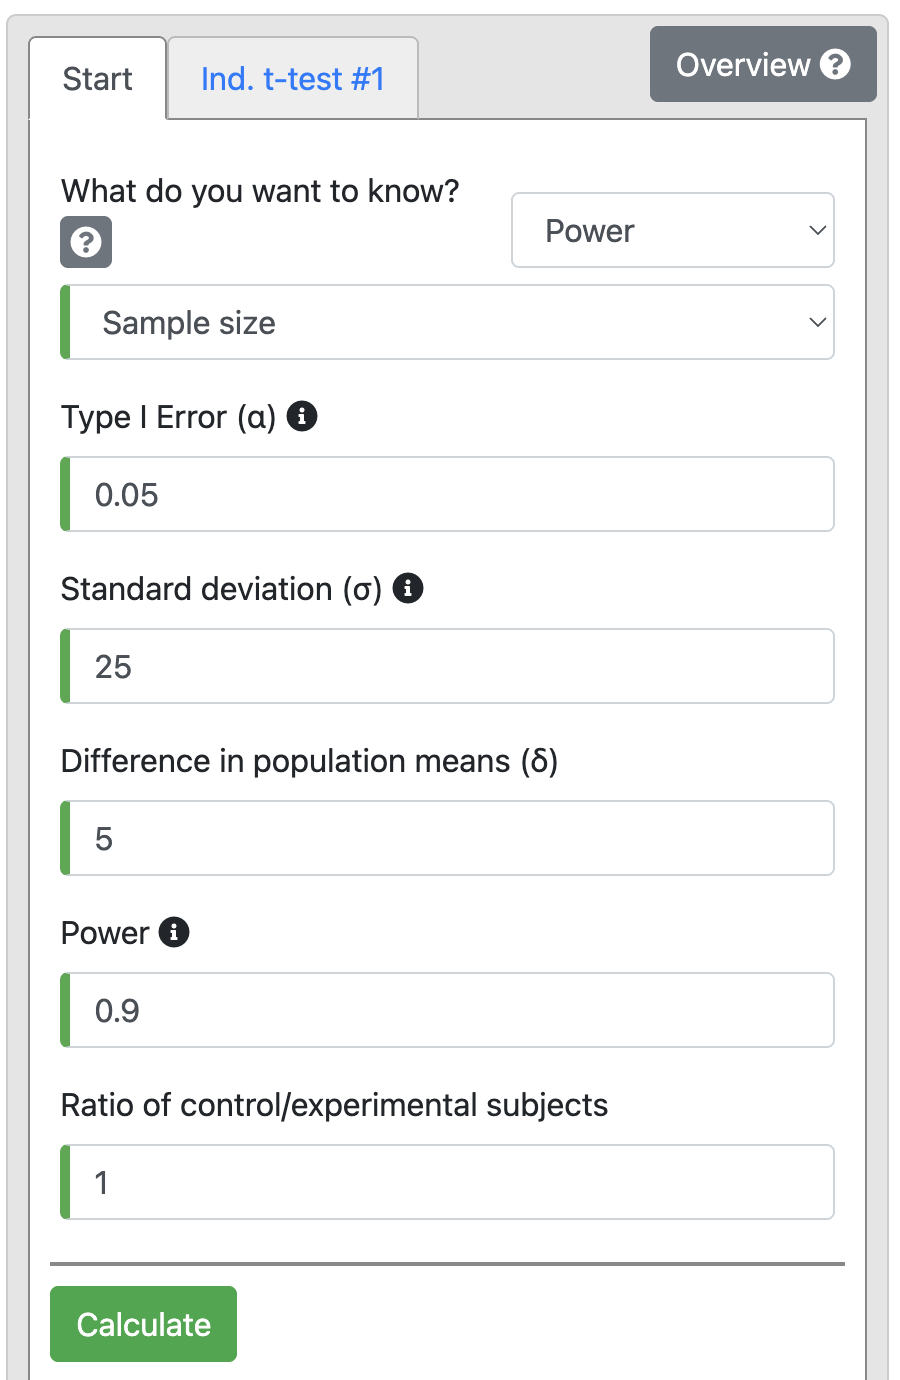
\includegraphics[width=0.4\linewidth,height=\textheight,keepaspectratio]{img/mod10/PS/mod10-twomeans-01.png}

\subsubsection{Output 10.2}\label{output-10.2}

\pandocbounded{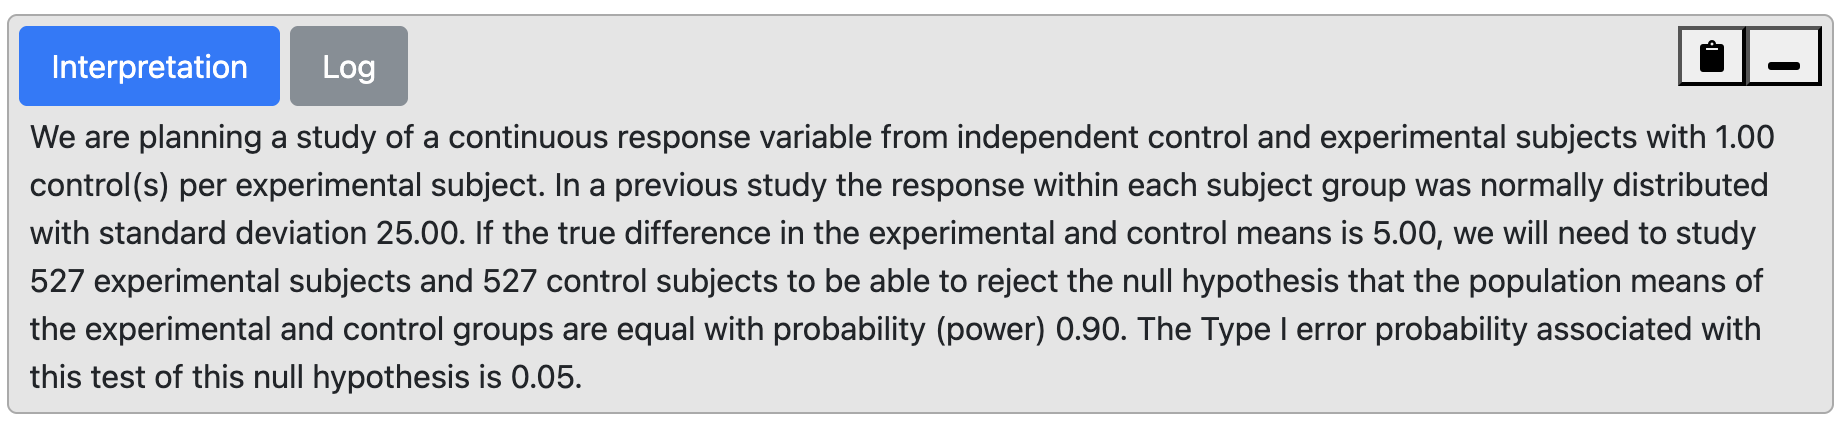
\includegraphics[keepaspectratio]{img/mod10/PS/mod10-twomeans-02.png}}

From the output, we can see that with 90\% power we will need 527
participants in each group, i.e., 1054 participants in total.

If the above were carried out by taking baseline measures of systolic
blood pressure, and then again when the women were taking the OC pills,
it would be a matched-pair study. Computing sample sizes for paired
studies requires an estimate of the correlation between the paired
observations, or an estimate of the standard deviation of the
differences. Calculating sample sizes for paired studies is a little
more complex than for independent studies, and is outside the scope of
this course.

\section{Detecting the difference between two
proportions}\label{detecting-the-difference-between-two-proportions}

The statistical test for deciding if there is a significant difference
between two independent proportions is a Pearson's chi-squared test
(Module 7).

Other than the power and alpha required for the test, the expected
prevalence or incidence rate of the outcome factor needs to be estimated
for each of the two groups being compared, based on what is known from
other studies or what is expected. Occasionally, we may not know the
expected proportion in one of the groups, e.g.~in a randomised control
trial of a novel intervention. In the sample size calculation for such a
study, we should instead justify the minimum expected difference between
the proportions based on what is important from a clinical or public
health perspective. Based on the minimum difference, we can then derive
the expected proportion for both groups. Note that the smaller the
difference, the larger the sample size required.

The sample size required in each group to observe a difference in two
independent proportions can be calculated using the \textbf{Dichotomous}
tab of PS.

\subsection{Worked Example 10.3}\label{wex10-3}

A health promotion campaign is being developed to reduce smoking in a
community, and will be tested in a randomised controlled trial. The
researchers would like to detect a reduction in smoking from 35\% to
25\%. How many participants should be recruited to detect a difference
at a 5\% significance level, with a power of 90\%?

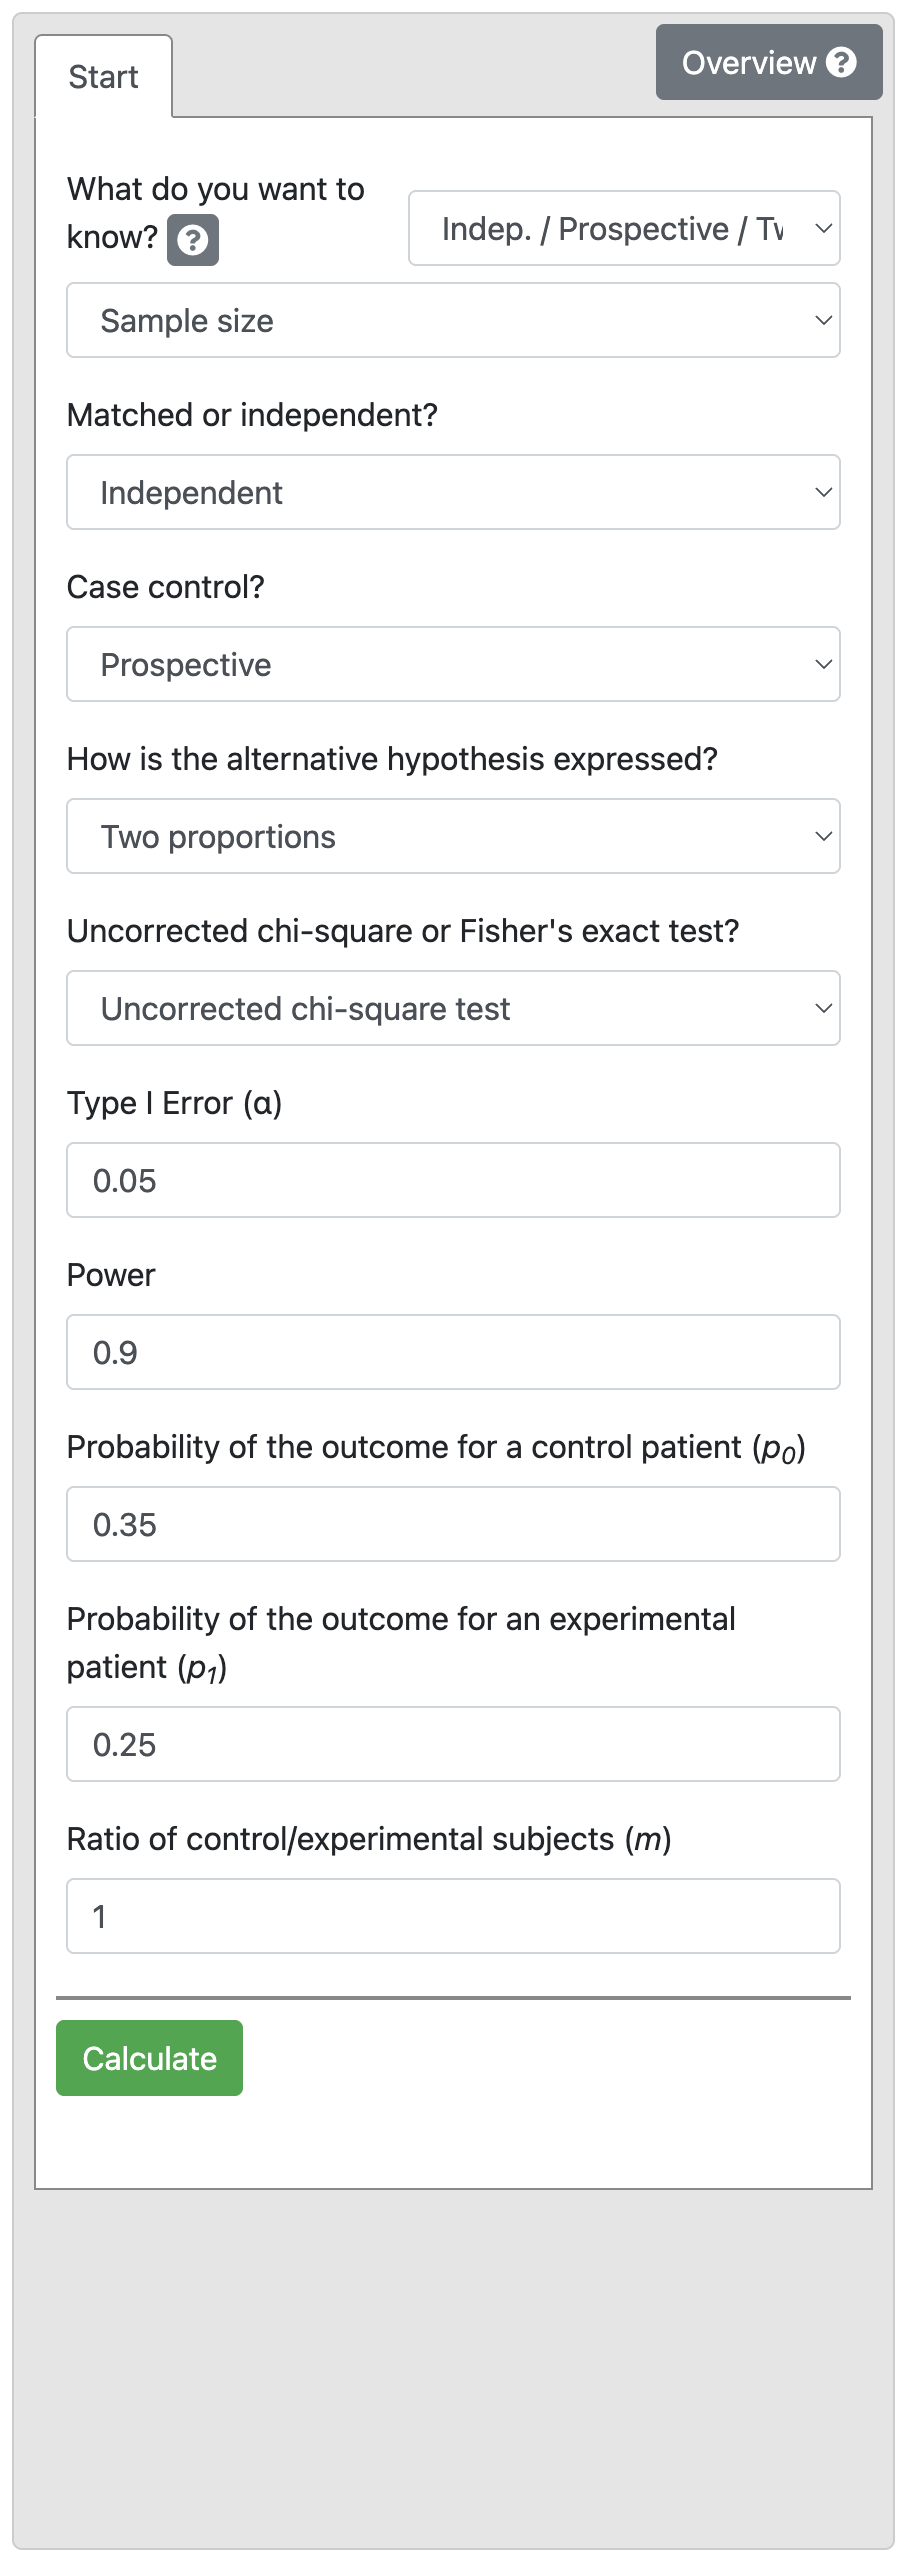
\includegraphics[width=0.4\linewidth,height=\textheight,keepaspectratio]{img/mod10/PS/mod10-twoprop-01.png}

\subsubsection*{Output 10.3: Sample size calculation for two independent
proportions}\label{output-10.3-sample-size-calculation-for-two-independent-proportions}
\addcontentsline{toc}{subsubsection}{Output 10.3: Sample size
calculation for two independent proportions}

\pandocbounded{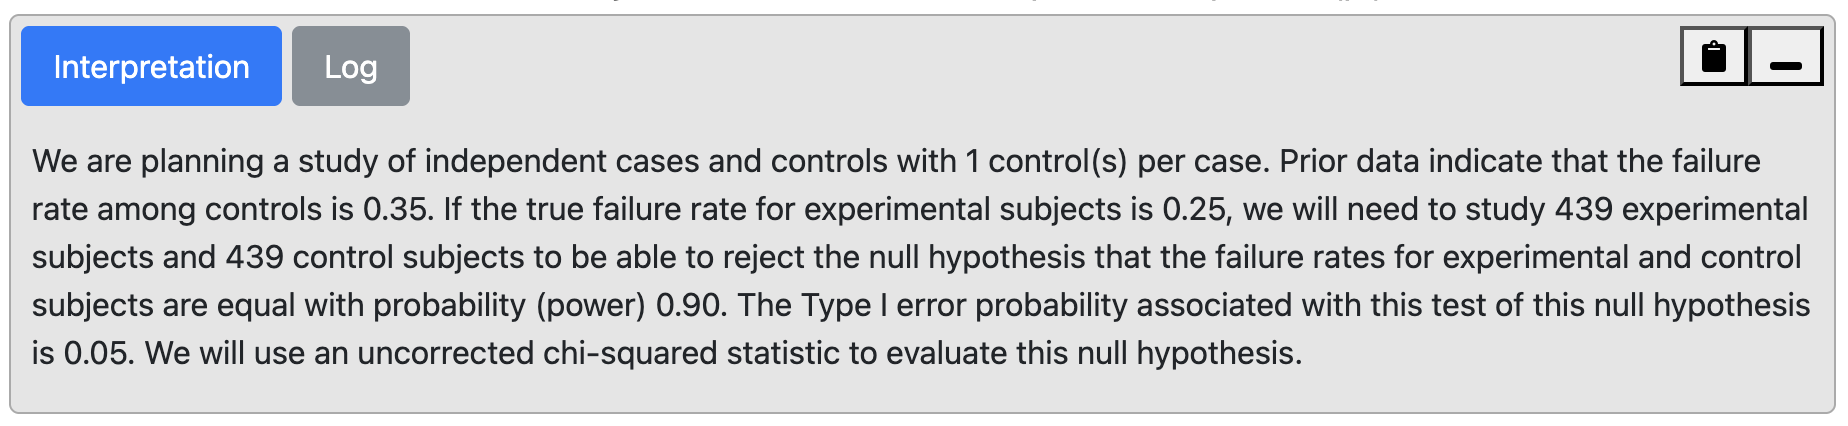
\includegraphics[keepaspectratio]{img/mod10/PS/mod10-twoprop-02.png}}

From Output 10.3, we see that we would need 439 intervention and 439
control participants (i.e.~a total sample size of 878 participants).

\section{Detecting an association using a relative
risk}\label{detecting-an-association-using-a-relative-risk}

The relative risk is used to describe the association between an
exposure and an outcome variable if the sample has been randomly
selected from the population. This statistic is often used to describe
the effect or association of an exposure in a cross-sectional or cohort
study or the effect/association of a treatment in an randomised
controlled trial. To estimate the sample size required for the RR to
have a statistically significant P value, i.e.~to show a significant
association, we need to define: - the size of the RR that is considered
to be of clinical or public health importance; - the event rate (rate of
outcome) among the group who are not exposed to the factor of interest
(reference group); - the desired level of significance (usually 0.05); -
the desired power of the study (usually 80\% or 90\%).

In general, a RR of 2.0 or greater is considered to be of public health
importance, however, a smaller RR can be important when exposure is
high. For example, there may be a relatively small risk of respiratory
infection among young children with a parent who smokes (RR
\textasciitilde{} 1.2). If 25\% of children are exposed to smoking in
their home, then the high exposure rate leads to a very large number of
children who have preventable respiratory infections across the
community.

\subsection{Worked Example 10.4}\label{wex10-4}

A study is planned to investigate the effect of an environmental
exposure on the incidence of a certain common disease. In the general
(unexposed) population the incidence rate of the disease is 50\% and it
is assumed that the incidence rate would be 75\% in the exposed
population. Thus the relative risk of interest would be 1.5 (i.e.~0.75 /
0.50). We want to detect this effect with 90\% power at a 5\% level of
significance.

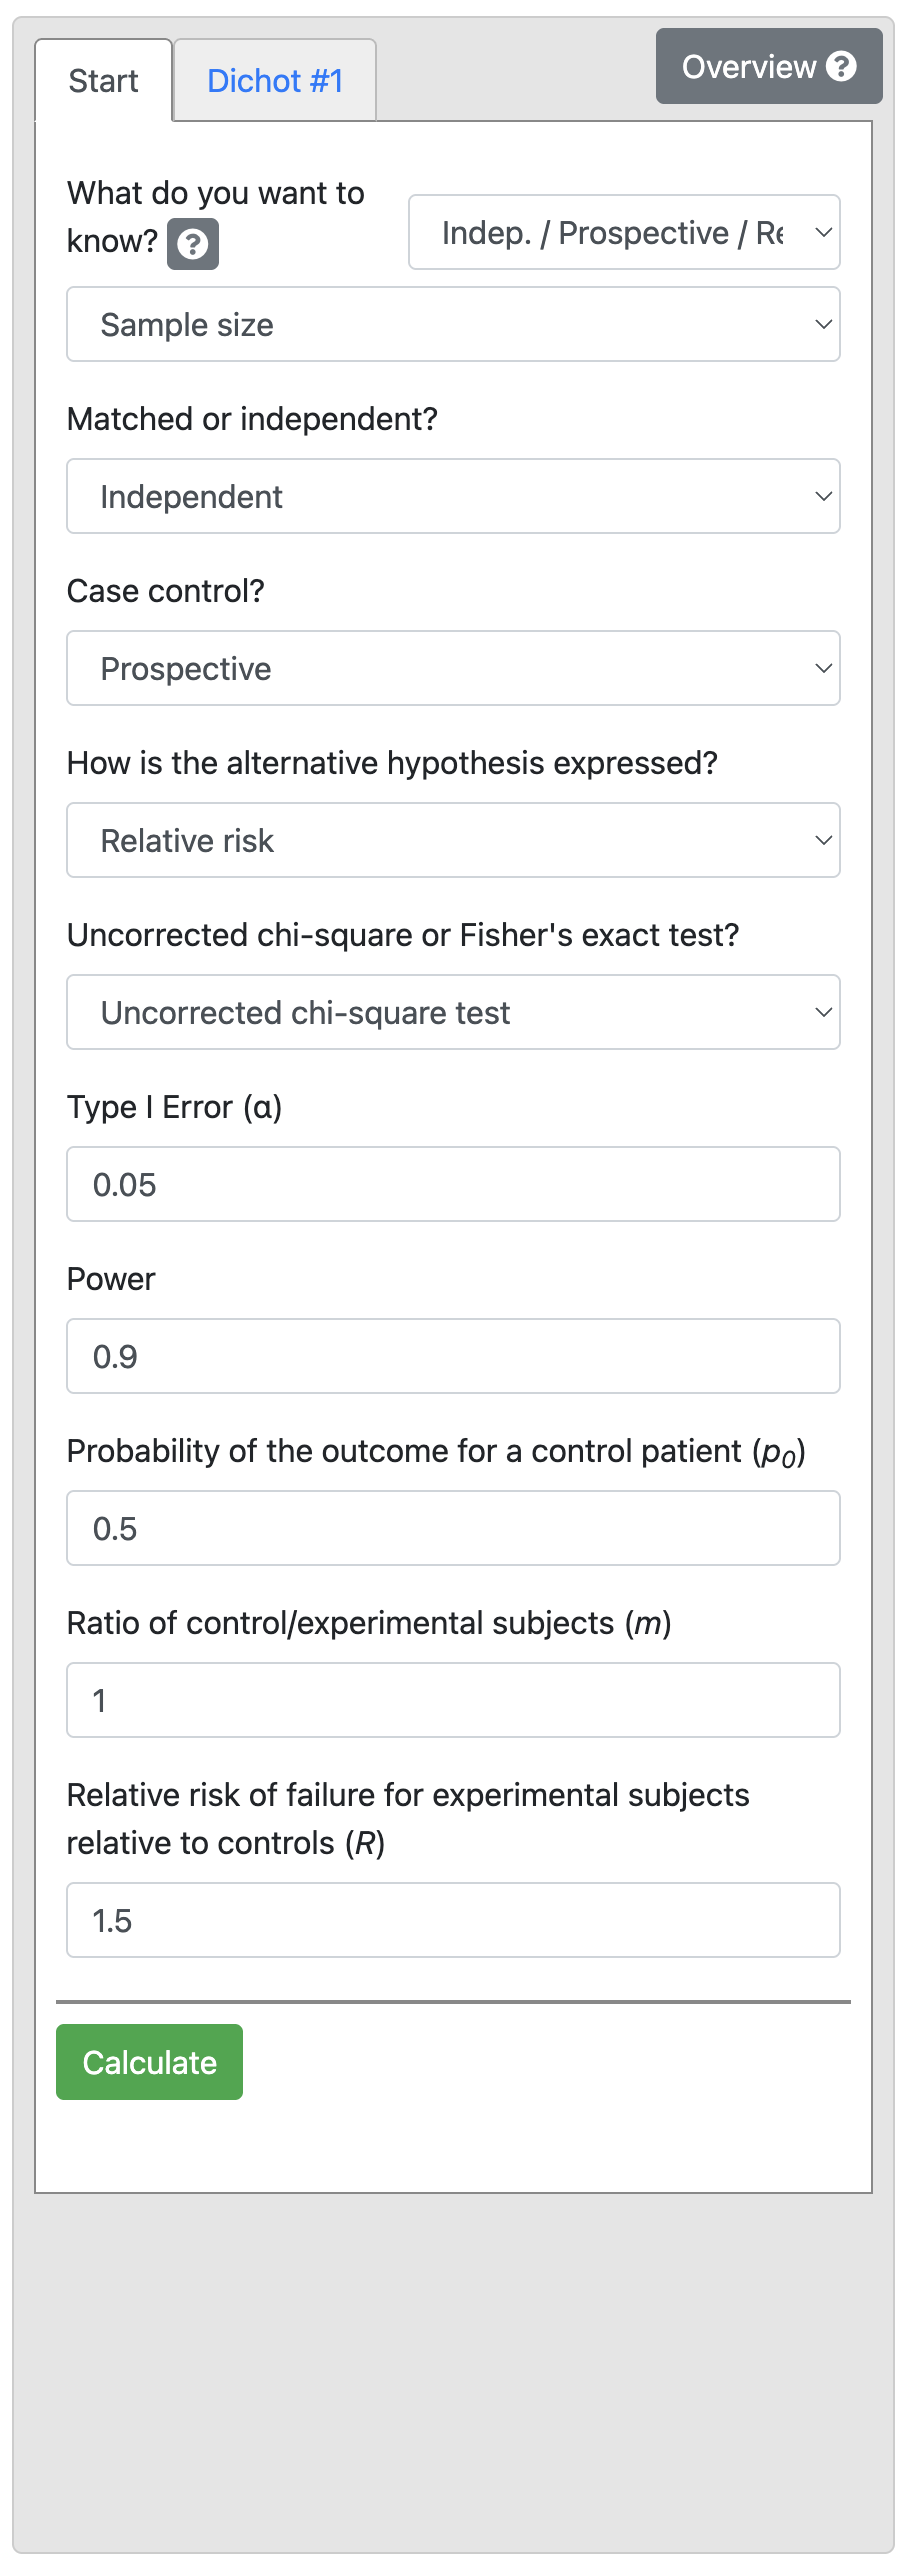
\includegraphics[width=0.4\linewidth,height=\textheight,keepaspectratio]{img/mod10/PS/mod10-rr-01.png}

\subsubsection{Output 10.4: Sample size calculation for relative
risk}\label{output-10.4-sample-size-calculation-for-relative-risk}

\pandocbounded{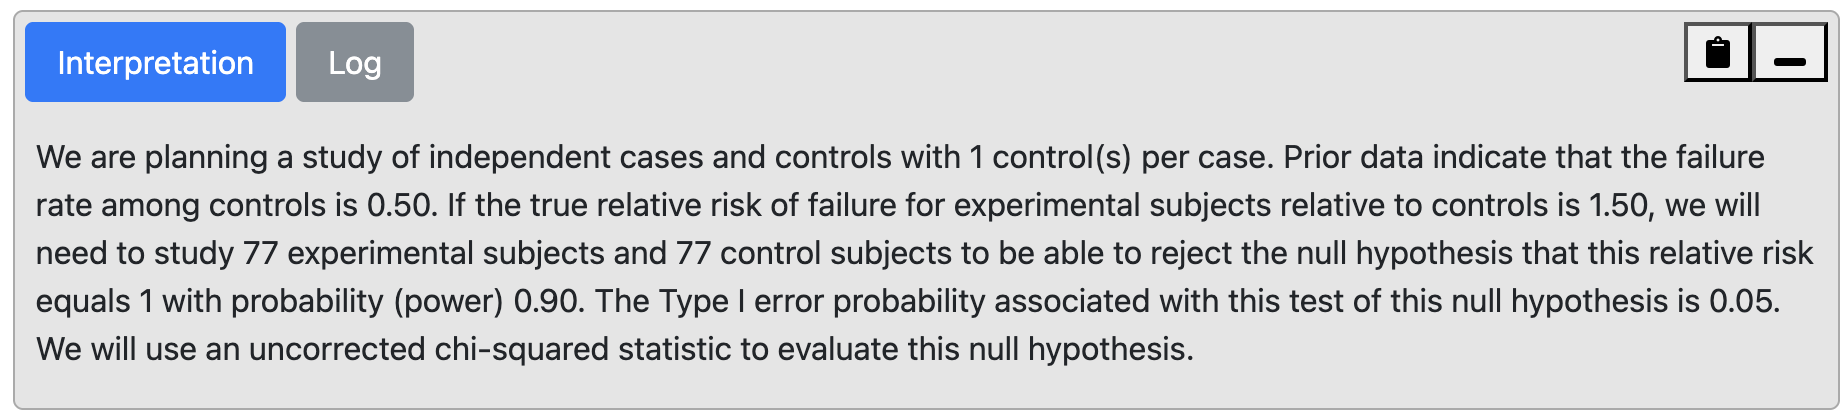
\includegraphics[keepaspectratio]{img/mod10/PS/mod10-rr-02.png}}

From Output 10.4, we can see that for a control proportion of 0.5 and RR
of 1.5, we need a total sample size of 154, that is 77 people would be
needed in each of the exposure groups.

\section{Detecting an association using an odds
ratio}\label{detecting-an-association-using-an-odds-ratio}

If we are designing a case-control study, the appropriate measure of
effect is an odds ratio. The method for estimating the sample size
required to detect an odds ratio of interest is slightly different to
that for the relative risk. However, the same parameters are required
for the estimation:

\begin{itemize}
\tightlist
\item
  the minimum OR to be considered clinically important;
\item
  the proportion of exposed among the control group;
\item
  the desired level of significance (usually 0.05);
\item
  the desired power of the study (usually 80\% or 90\%).
\end{itemize}

\subsection{Worked Example 10.5}\label{wex10-5}

A case-control study is designed to examine an association between an
exposure and outcome factor. Existing literature shows that 30\% of the
controls are expected to be exposed. We want to detect a minimum OR of
2.0 with 90\% power and 5\% level of significance.

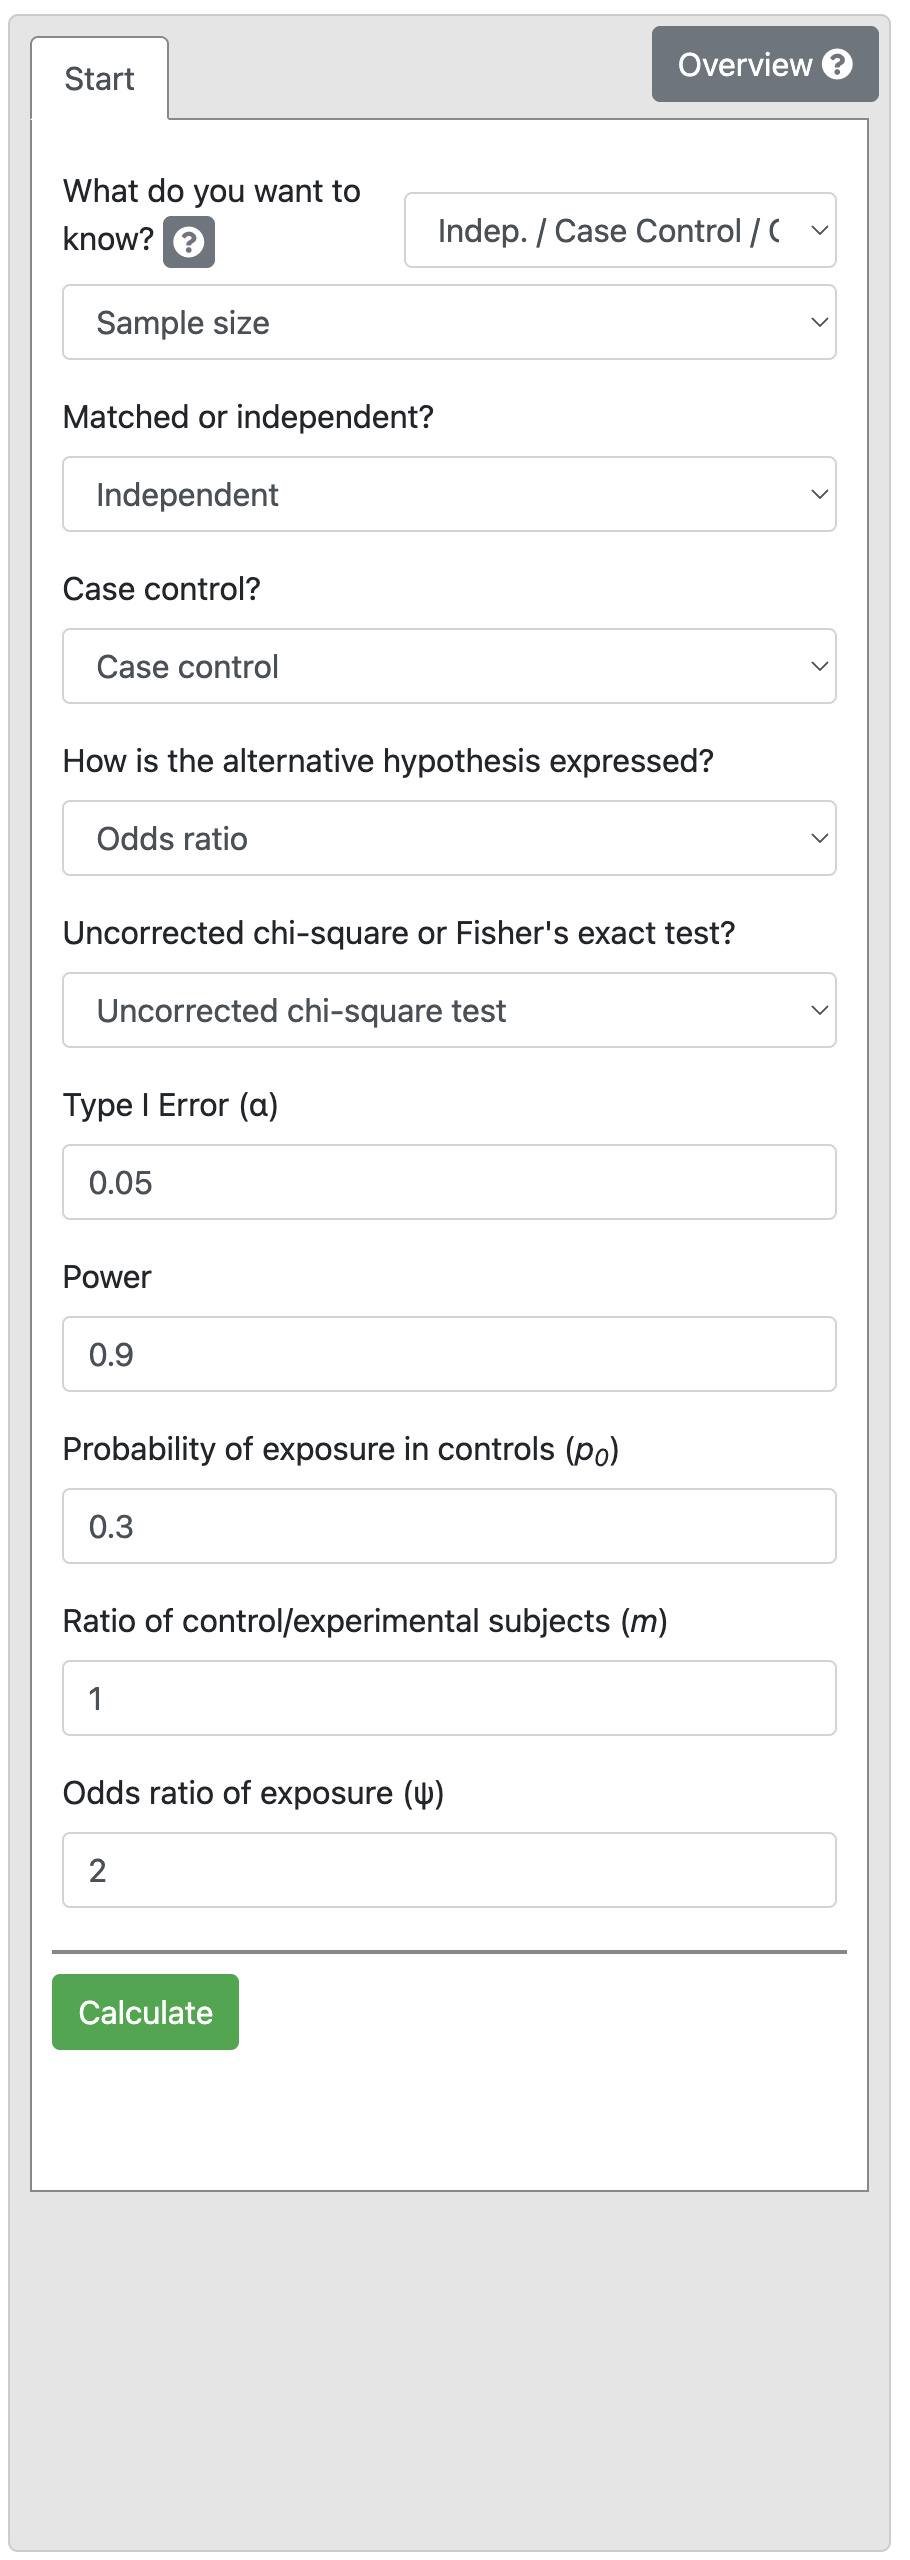
\includegraphics[width=0.4\linewidth,height=\textheight,keepaspectratio]{img/mod10/PS/mod10-or-01.png}

\subsubsection{Output 10.5}\label{output-10.5}

\pandocbounded{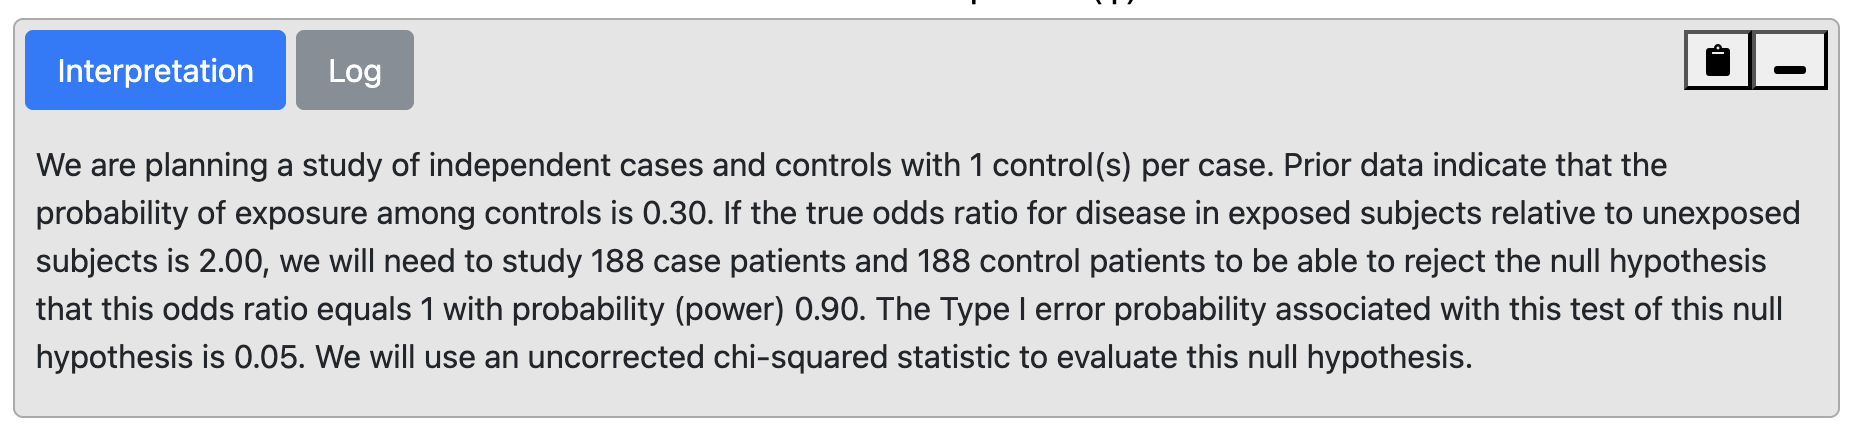
\includegraphics[keepaspectratio]{img/mod10/PS/mod10-or-02.png}}

We find that 188 controls and 188 cases are required i.e.~a total of 376
participants.

This sample size would be smaller if we increased the effect size (OR)
or reduced the study power to 80\%. You could try this yourself (answer:
141 per group if power is reduced to 80\%).

\section{Factors that influence
power}\label{factors-that-influence-power}

\subsection{Dropouts}\label{dropouts}

It is common to increase estimated sample sizes to allow for drop-outs
or non-response. To account for drop-outs, the estimated sample size can
be divided by (1 minus the dropout rate). Consider the following case:

\begin{itemize}
\tightlist
\item
  n-completed: the number who will complete the study (i.e.~n after
  drop-out)
\item
  n-recruited: the number who should be recruited (i.e.~n before
  drop-out)
\item
  d: drop-out rate (as a proportion - i.e.~a number between 0 and 1)
\end{itemize}

Then n-completed = n-recruited × (1 - d)

Re-arranging this formula gives: n-recruited = n-completed ÷ (1 - d).

\subsection{Unequal groups}\label{unequal-groups}

Many factors that come into play in a study can reduce the estimated
power of a study. In clinical trials, it is not unusual for recruitment
goals to be much harder to achieve than expected and therefore for the
target sample size to be impossible to realise within the timeframe
planned for recruitment.

In case-control studies, the number of potential case participants
available may be limited but study power can be maintained by enrolling
a greater number of controls than cases. Or in an experimental study,
more participants may be randomised to the new treatment group to test
its effects accurately when much is known about the effect of standard
care and a more precise estimate of the new treatment effect is
required.

However, there is a trade-off between increasing the ratio of group size
and the total number that needs to be enrolled. Consider Worked Example
10.5: selecting an equal number of controls and cases would require 188
cases and 188 controls, a total of 376 participants.

We may want to reduce the number of cases required, by selecting 2
controls for every case. Selecting 2 controls (N1) per case (N2) would
require 140 cases and 280 controls, a total of 420 participants. We can
extend this example and investigate the impact of changing the ratio of
controls per case.

\newpage

\begin{table}
\caption{The effect of unequal groups on Worked Example 10.5}\tabularnewline

\centering
\begin{tblr}[         %% tabularray outer open
]                     %% tabularray outer close
{                     %% tabularray inner open
colspec={Q[]Q[]Q[]Q[]},
hline{2}={1-4}{solid, black, 0.05em},
hline{1}={1-4}{solid, black, 0.08em},
hline{12}={1-4}{solid, black, 0.08em},
}                     %% tabularray inner close
Controls per case & Number of cases required & Number of controls required & Total participants required \\
1 & 188 & 188 & 376 \\
2 & 140 & 280 & 420 \\
3 & 124 & 372 & 496 \\
4 & 115 & 460 & 575 \\
5 & 111 & 555 & 666 \\
6 & 107 & 642 & 749 \\
7 & 105 & 735 & 840 \\
8 & 103 & 824 & 927 \\
9 & 102 & 918 & 1020 \\
10 & 101 & 1010 & 1111 \\
\end{tblr}
\end{table}

This can be visualised graphically, as in
Figure~\ref{fig-unequal-controls}.

\begin{figure}

\centering{

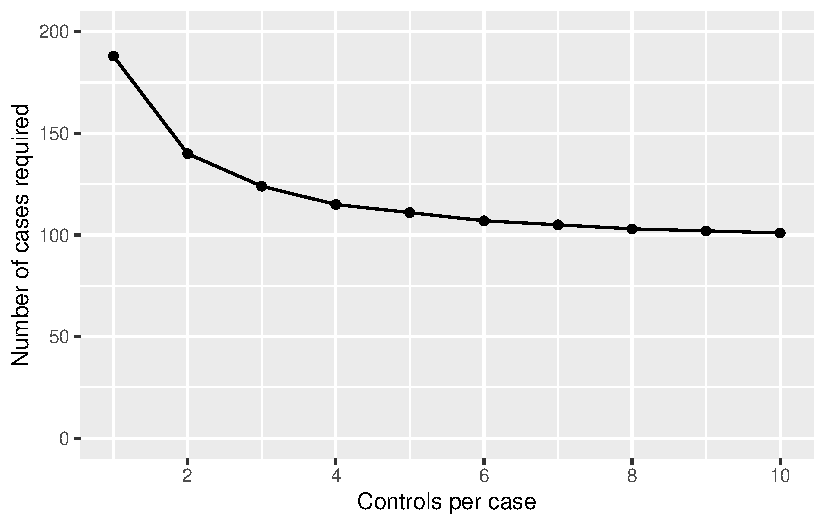
\includegraphics[width=0.66\linewidth,height=\textheight,keepaspectratio]{10-sample-size_files/figure-pdf/fig-unequal-controls-1.pdf}

}

\caption{\label{fig-unequal-controls}Increasing the number of controls
per case}

\end{figure}%

We can see that the number of cases required drops off if we go from 1
to 2 controls per case, and again from 2 to 3 controls per case. Once we
go from 3 to 4 controls per case, we only reduce the number of cases by
9 (124 vs 115 cases), but at an increase of 88 (372 vs 460) controls.
Clearly, this reduction in cases is not offset by the extra controls
required.

\section{Limitations in sample size
estimations}\label{limitations-in-sample-size-estimations}

In this module we have seen how to use a sample size calculator to
estimate the sample size requirement of a study given the statistical
test that will be used and the expected characteristics of the sample.
However, once a study is running, it is not unusual for sample size to
be compromised by the lack of research resources, difficulties in
recruiting participants or, in a clinical trial, participants wanting to
change groups when information about the new experimental treatment
rapidly becomes available in the press or on the internet.

One approach that is increasingly being used is to conduct a blinded
interim analysis say when 50\% of the total data that are planned have
been collected. In this, a statistician external to the research team
who is blinded to the interpretation of the group code is asked to
measure the effect size in the data with the sole aim of validating the
sample size requirement. It is rarely a good idea to use an interim
analysis to reduce the planned sample size and terminate a trial early
because the larger the sample size, the greater the precision with which
the treatment effect is estimated. However, interim analyses are useful
for deciding whether the sample size needs to be increased in order to
answer the study question and avoid a Type II error.

\section{Summary}\label{summary-2}

In this module we have discussed the importance of conducting a clinical
or epidemiological study with enough participants so that an effect or
association can be identified if it exists (i.e.~study power), and how
this has to be balanced by the need to not enrol more participants than
necessary because of resource issues. We have looked at the parameters
that need to be considered when estimating the sample size for different
studies and have used a look-up table to estimate required sample size
for a prevalence study and a sample size calculator to estimate
appropriate sample sizes in epidemiological research under the most
straightforward situations. The common requirement in all the situations
is that the researchers need to specify the minimum effect measure
(e.g.~difference in means, OR, RR etc) they want to detect with a given
probability (usually 80\% to 90\%) at a certain level of significance
(usually P\textless0.05). The ultimate decision on the sample size
depends on a compromise among different objectives such as power,
minimum effect size, and available resources. To make the final
decision, it is helpful to do some trial calculations using revised
power and the minimum detectable effect measure.

\newpage{}

\bookmarksetup{startatroot}

\chapter*{Software notes}\label{software-notes}
\addcontentsline{toc}{chapter}{Software notes}

\markboth{Software notes}{Software notes}

In this module, we will demonstrate the use of an online calculator
called PS, available at https://cqsclinical.app.vumc.org/ps/ While
sample size calculations can be conducted in R (using the \texttt{EpiR}
and \texttt{pwr} packages in particular), there is currently an
inconsitency in \texttt{EpiR} which means that I do not recommend this
package.

\pandocbounded{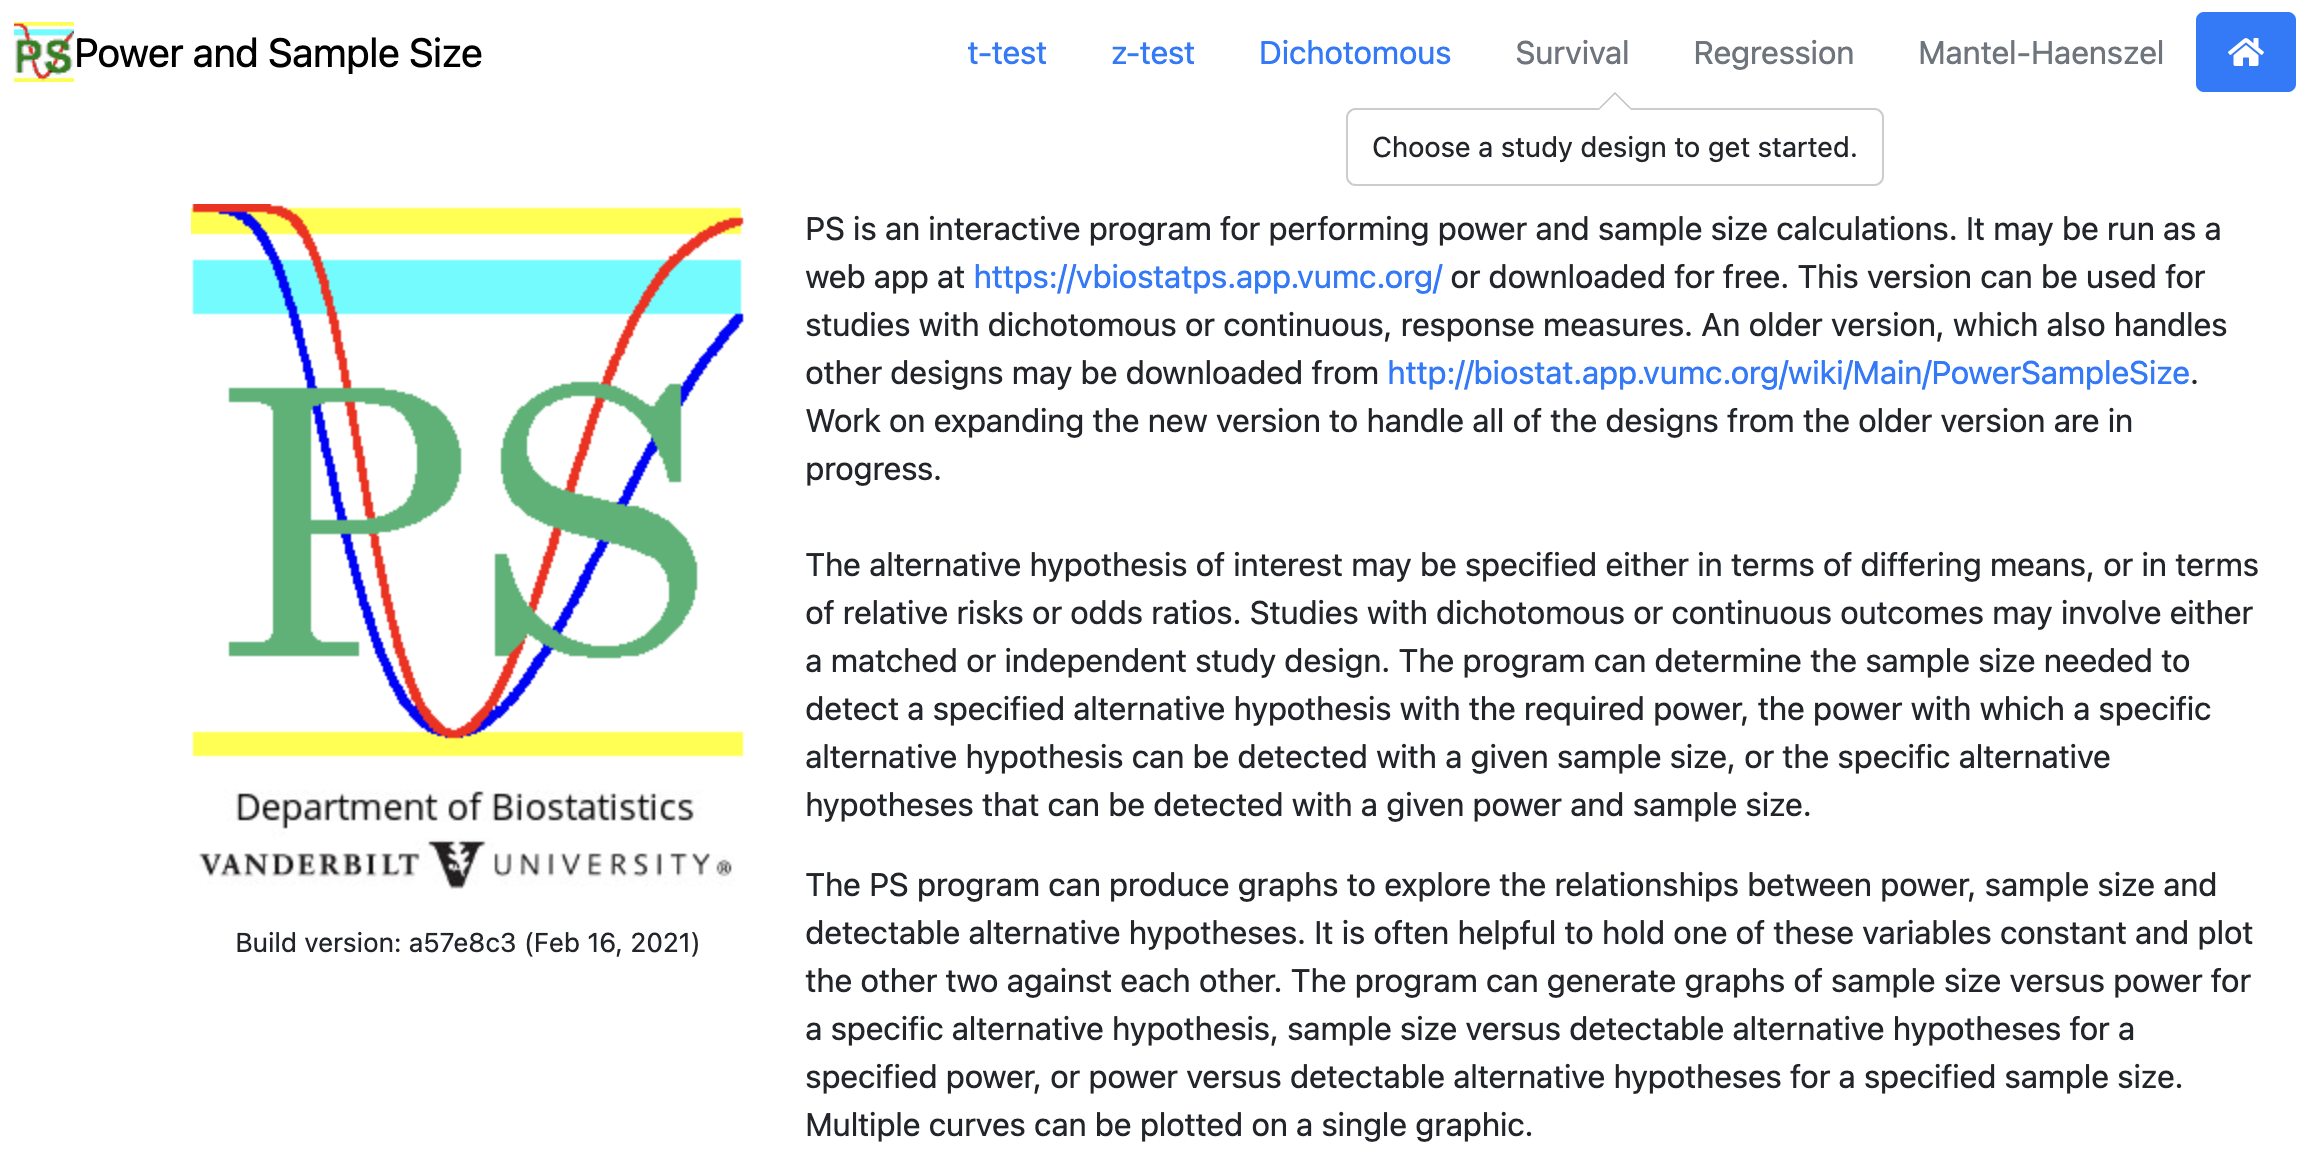
\includegraphics[keepaspectratio]{img/mod10/PS/mod10-ps-01.png}}

The web-app allows for a variety of variable types; we will focus on
\textbf{t-test} and \textbf{Dichotomous} analyses.

\section{Sample size calculation for two independent samples
t-test}\label{sample-size-calculation-for-two-independent-samples-t-test}

To do the problem discussed in Worked Example 10.2, choose
\textbf{t-test \textgreater{} Independent}. Choose \textbf{Power} in the
first drop-down, and then choose \textbf{Sample size}:

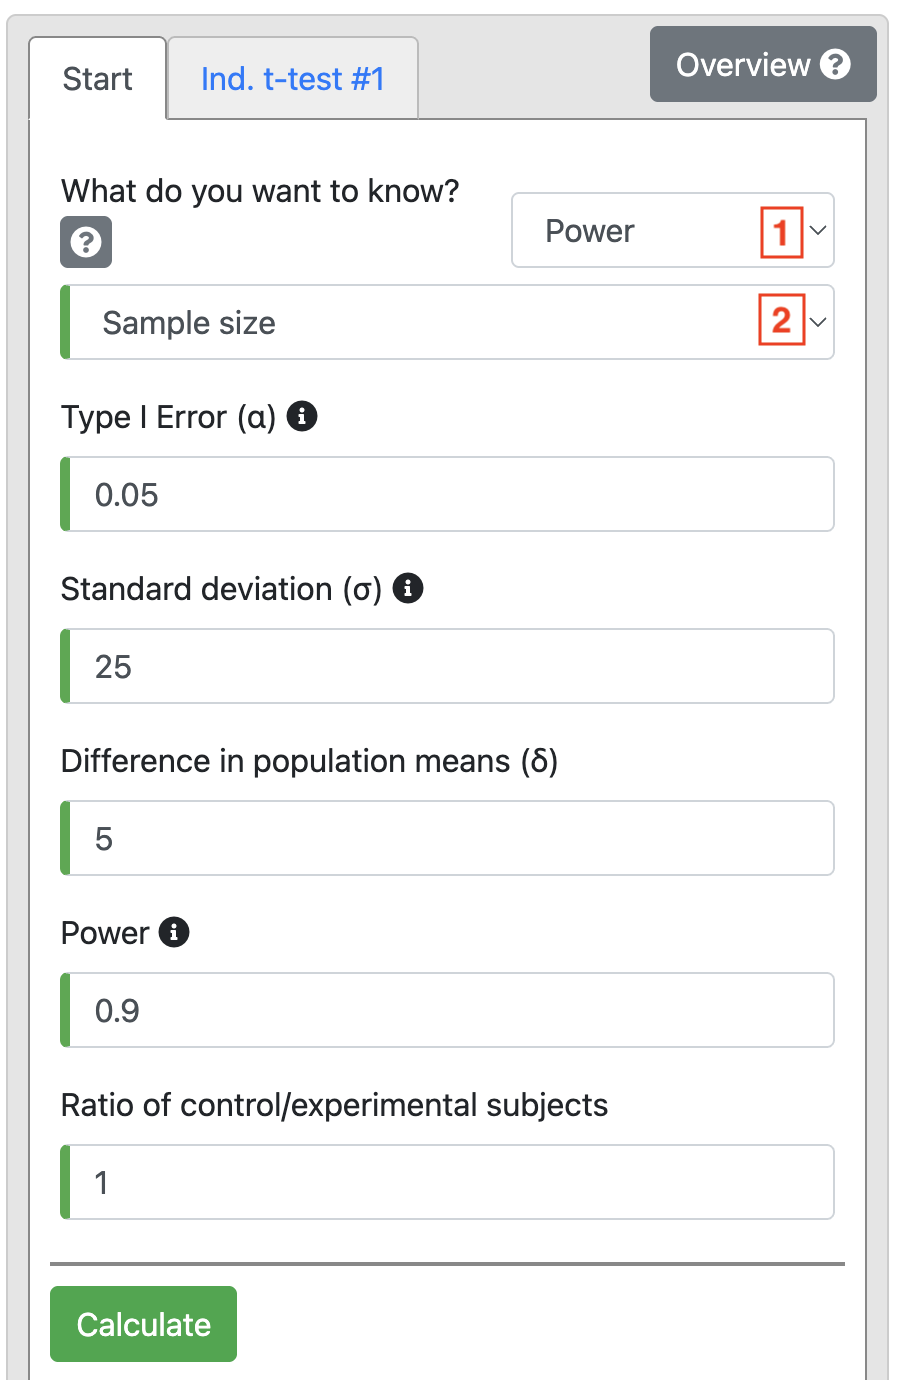
\includegraphics[width=0.4\linewidth,height=\textheight,keepaspectratio]{img/mod10/PS/mod10-twomeans-03.png}

Based on the information in Worked Example 10.2, change \textbf{Power}
to \texttt{0.9} and enter \texttt{25} as the \textbf{Standard deviation
(σ)}. We are interested in detecting a difference of 5 mmHg, so this is
entered as \textbf{Diference in population means (δ)}. We use equal
numbers in each group, so \textbf{Ratio} is entered as 1.

Click \textbf{Calculate} to produce Output 10.2.

\section{Sample size calculation for difference between two independent
proportions}\label{sample-size-calculation-for-difference-between-two-independent-proportions}

All sample size calculations for analyses based on 2-by-2 tables are
conducted under the \textbf{Dichotomous} tab, choosing:

\begin{itemize}
\tightlist
\item
  \textbf{Indep / Prospective / Two Prop.} for analyses based on
  estimating the difference in proportions;
\item
  \textbf{Indep / Prospective / Rel. Risk} for analyses based on
  estimating a relative risk;
\item
  \textbf{Indep / Case Control / Odds Ratio} for case-control studies.
\end{itemize}

To do the problem discussed in Worked Example 10.3, choose \textbf{Indep
/ Prospective / Two Prop.} and \textbf{Sample size} in the first two
drop-down options.

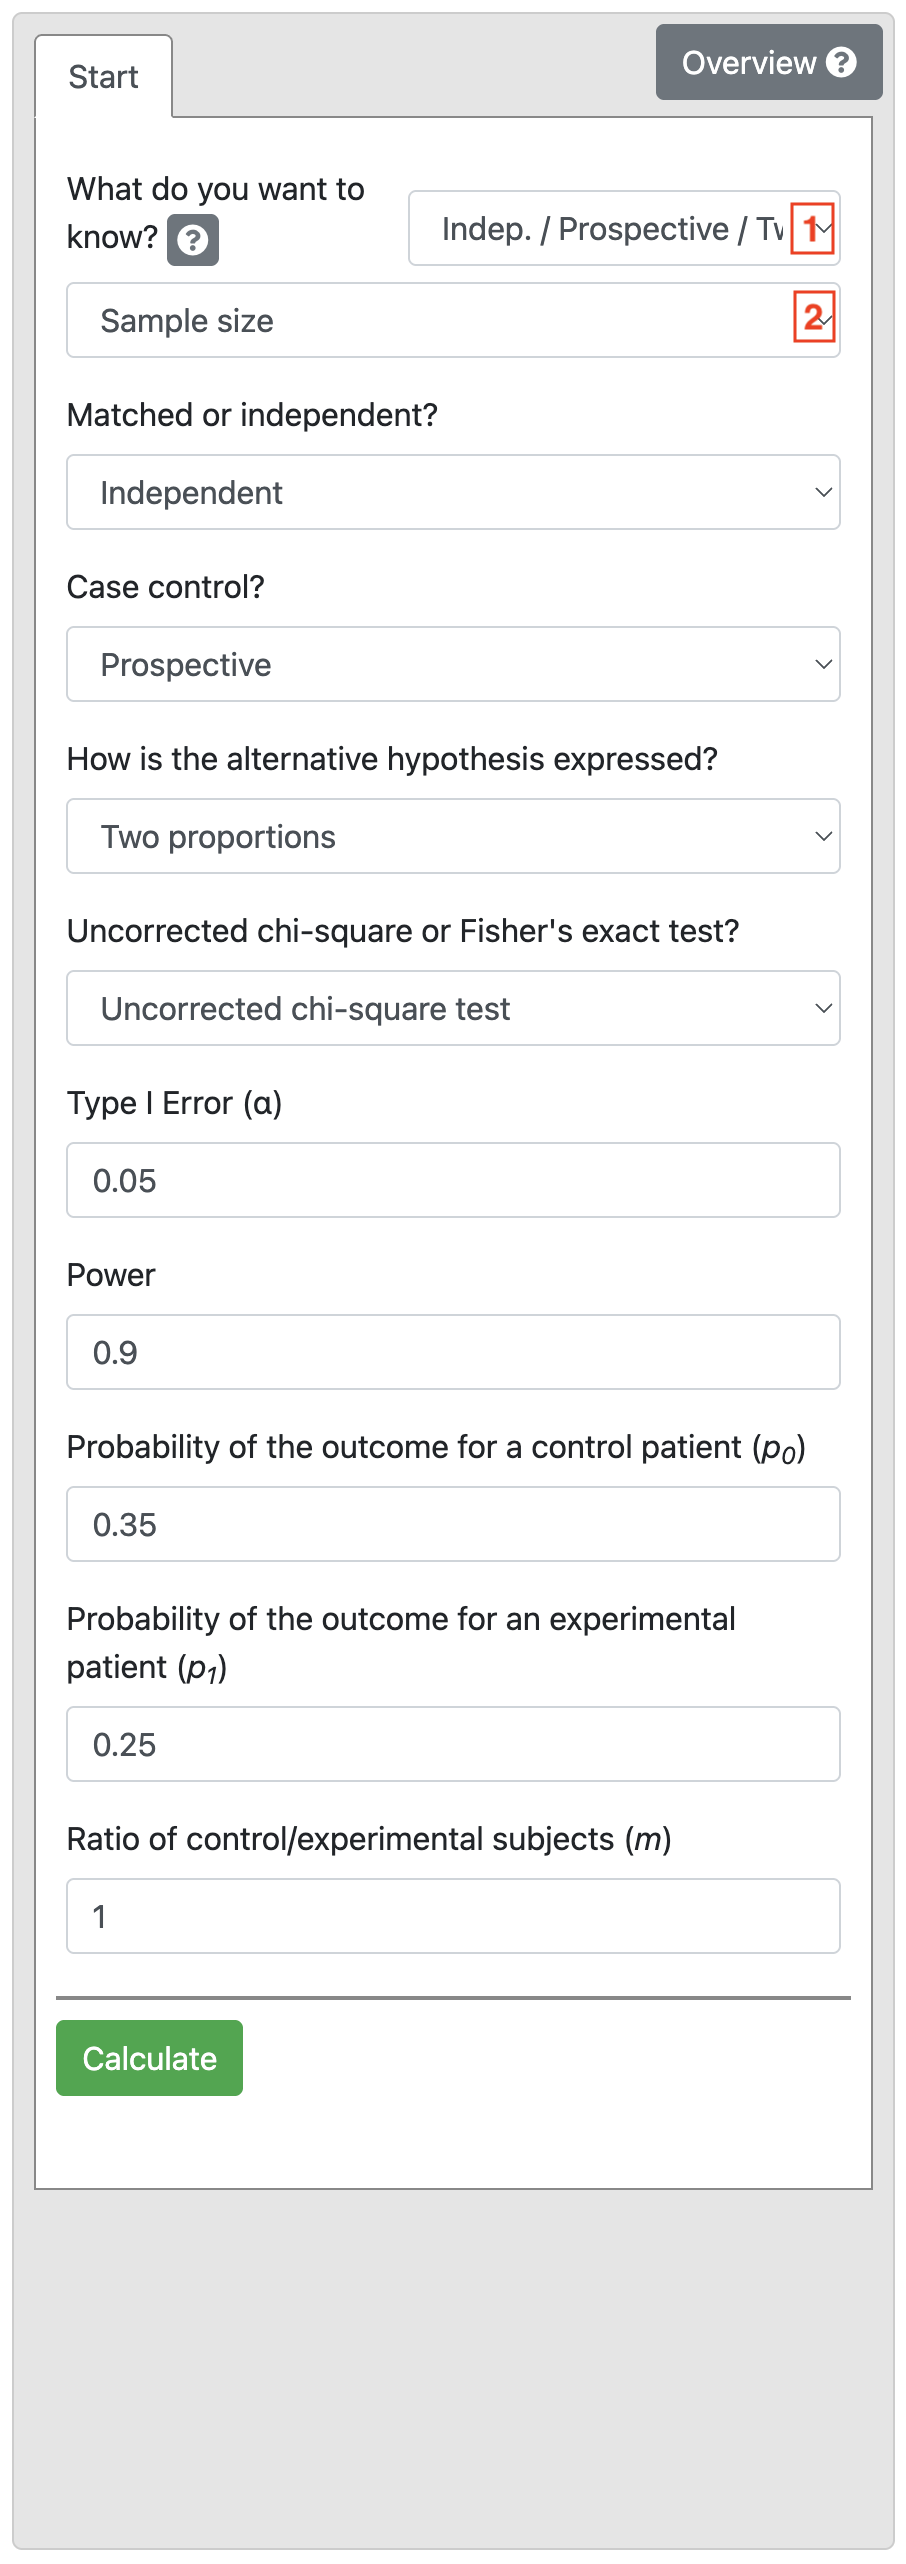
\includegraphics[width=0.4\linewidth,height=\textheight,keepaspectratio]{img/mod10/PS/mod10-twoprop-03.png}

Based on the information in Worked Example 10.5, the \textbf{Power} is
\texttt{0.9} and \textbf{Significance level} is \texttt{0.05}, and the
two proportions are entered as \texttt{0.35} and \texttt{0.2}. Define
equal numbers in each group (\textbf{Ratio} of \texttt{1}).

Click \textbf{Calculate} obtain Output 10.3.

Note: It doesn't matter if you swap the proportions for the
\textbf{Control} and \textbf{Experimental} group, you will get the same
result.

\section{Sample size calculation with a relative risk or odds
ratio}\label{sample-size-calculation-with-a-relative-risk-or-odds-ratio}

Using information from Worked Example 10.4, we select \textbf{Indep /
Prospective / Rel. Risk}, and enter \textbf{Power} as \texttt{0.9},
enter \texttt{0.5} as the \textbf{Probability of the outcome for a
control patient (p0)}. Finally, enter \texttt{1.5} as the
\textbf{Relative risk of failure for experimental subjects relative to
controls (R)} shown below:

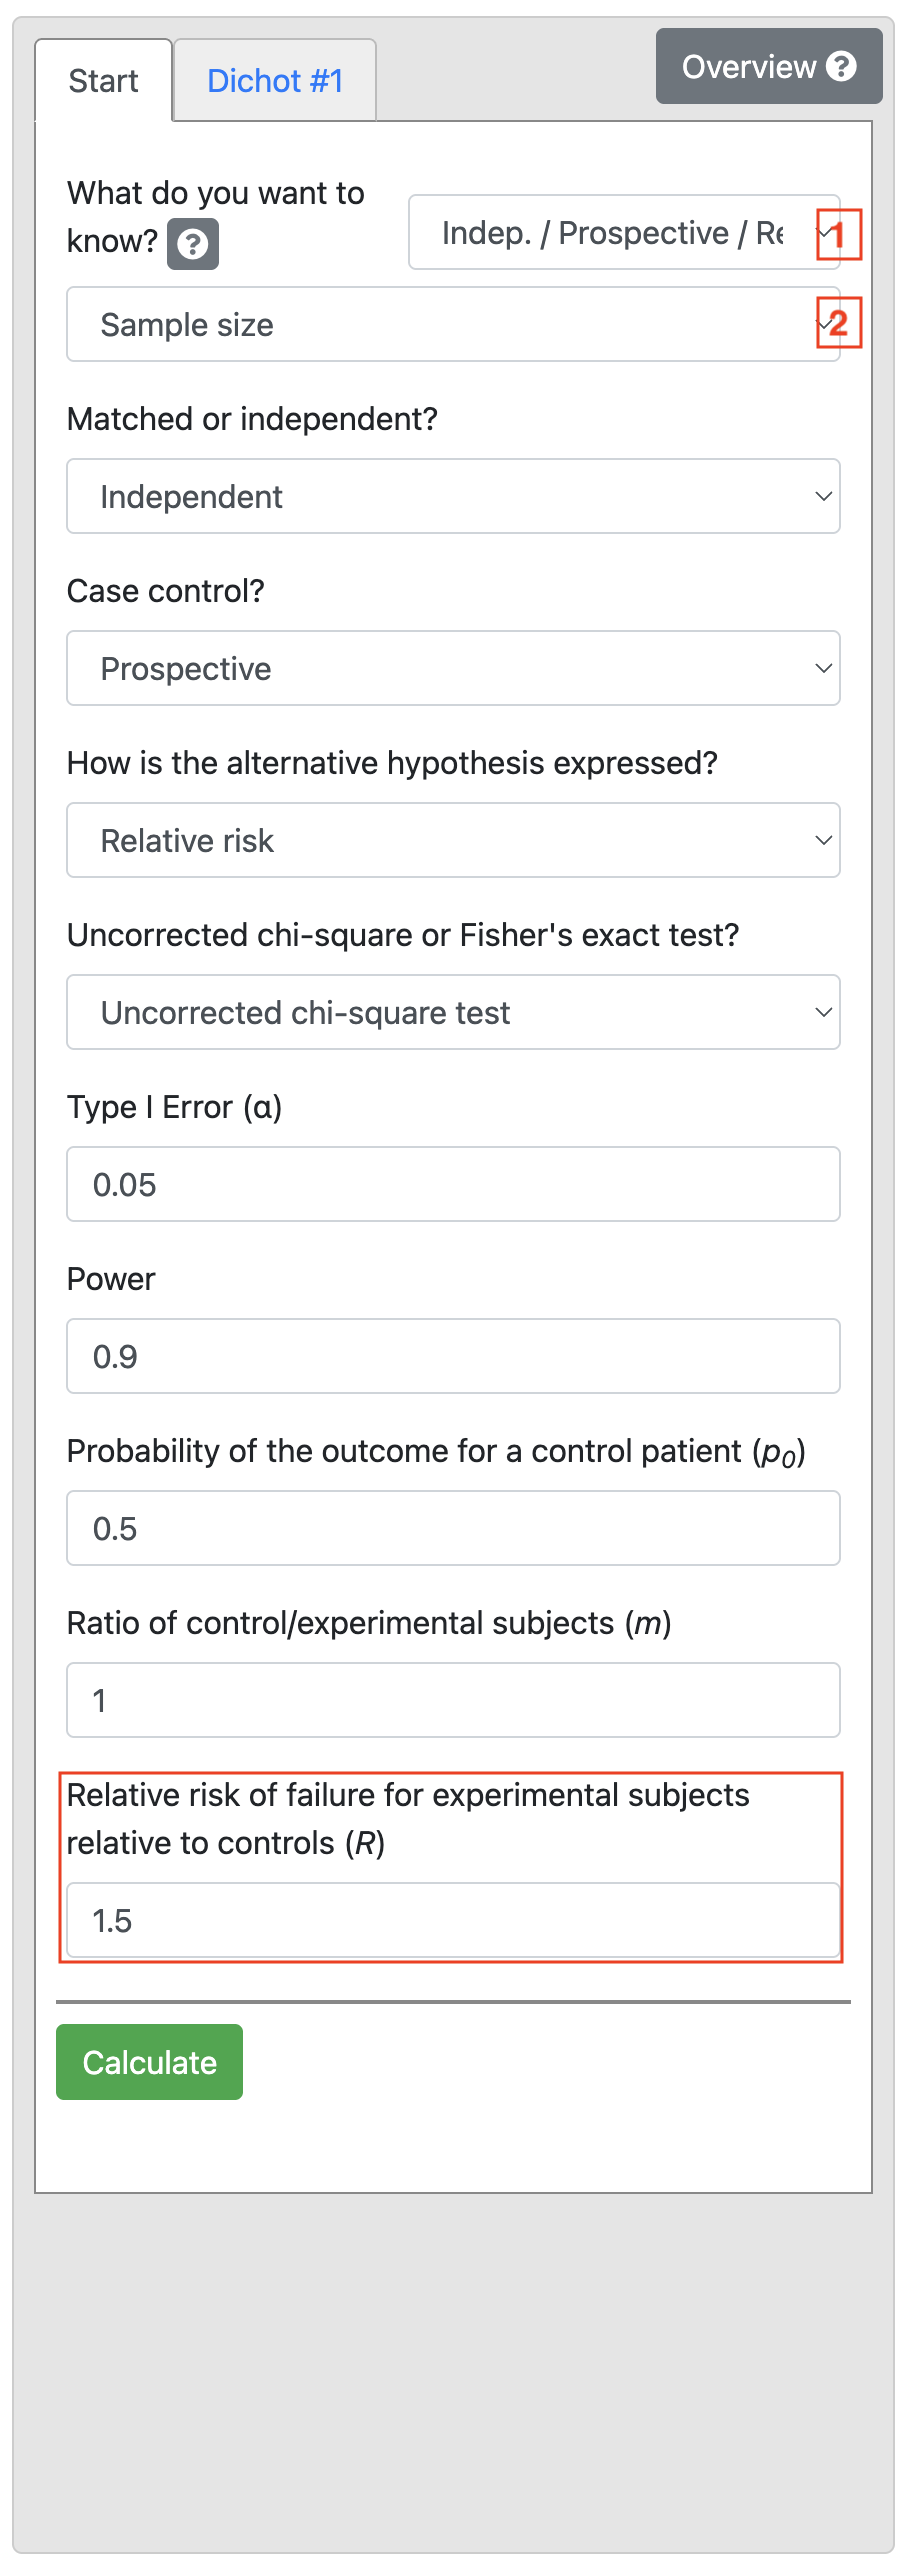
\includegraphics[width=0.4\linewidth,height=\textheight,keepaspectratio]{img/mod10/PS/mod10-rr-03.png}

Now we calculate the sample size for Worked Example 10.5. Select
\textbf{Indep / Case Control / Odds Ratio} and \textbf{Sample size}, and
enter \textbf{Power} as \texttt{0.9}, enter \texttt{0.3} as the
\textbf{Probability of exposure in controls (p0)}. Finally, enter
\texttt{2} as the \textbf{Odds ratio of exposure (ψ)} shown below:

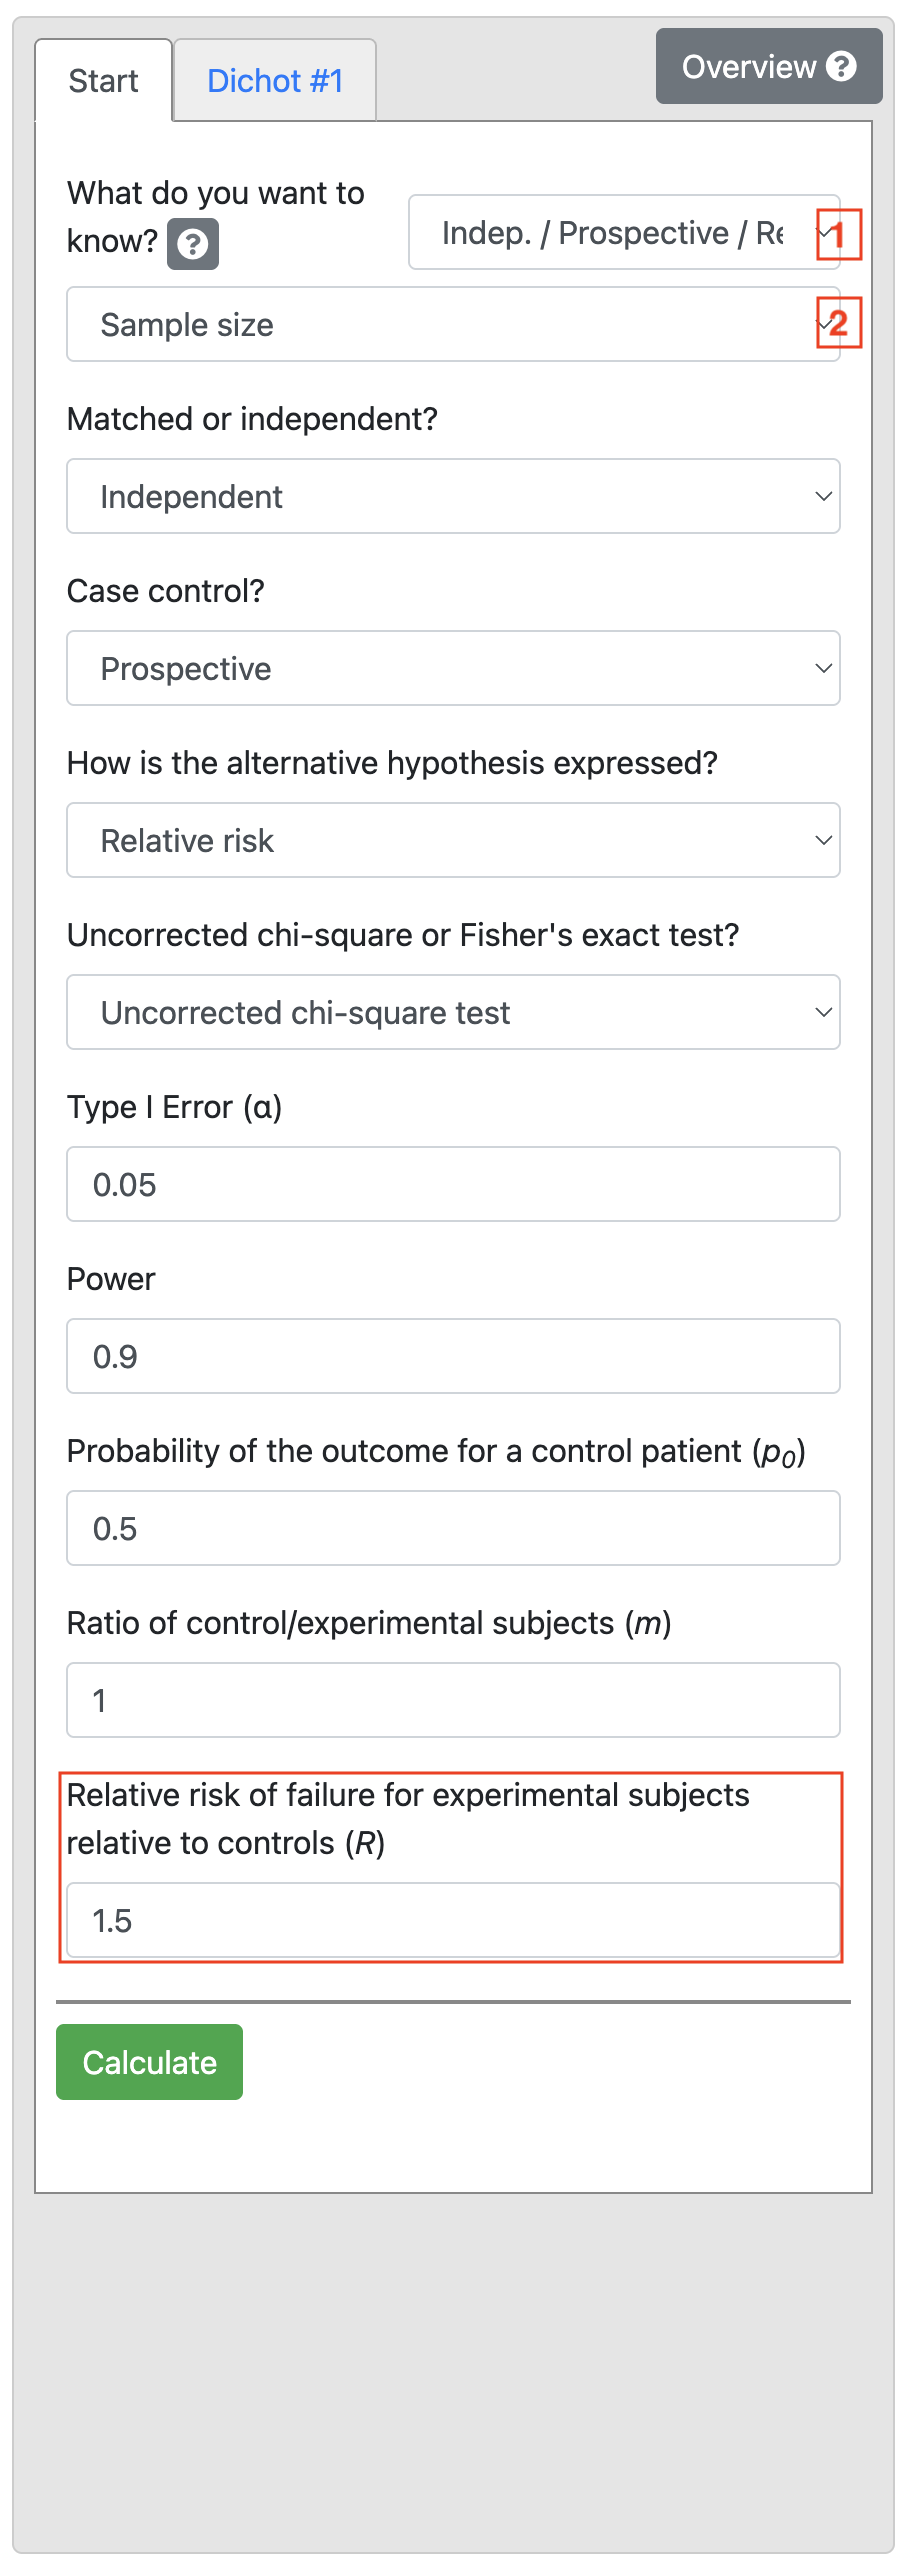
\includegraphics[width=0.4\linewidth,height=\textheight,keepaspectratio]{img/mod10/PS/mod10-rr-03.png}

\section{Estimating power or effect
size}\label{estimating-power-or-effect-size}

Note that in all PS examples provided here, we have chosen to estimate
the sample size (given the study power and effect size of interest). PS
also allows us to estimate the power (given the study sample size and
effect size) or the effect size (given the study sample size and power).

\bookmarksetup{startatroot}

\chapter*{Activities}\label{activities-9}
\addcontentsline{toc}{chapter}{Activities}

\markboth{Activities}{Activities}

\subsection*{Activity 10.1}\label{activity-10.1}
\addcontentsline{toc}{subsection}{Activity 10.1}

We are planning a study to measure the prevalence of a relatively rare
condition (say approximately 5\%) in children age 0-5 years in a remote
community.

\begin{enumerate}
\def\labelenumi{\alph{enumi})}
\tightlist
\item
  What type of study would need to be conducted?
\item
  Use the correct sample size table included in your notes to determine
  how many children would need to be enrolled for the confidence
  interval to be

  \begin{enumerate}
  \def\labelenumii{\roman{enumii}.}
  \tightlist
  \item
    2\%
  \item
    4\% around the prevalence?
  \end{enumerate}
\end{enumerate}

What would the resulting prevalence estimates and 95\% CIs be?

\subsection*{Activity 10.2}\label{activity-10.2}
\addcontentsline{toc}{subsection}{Activity 10.2}

We are planning an experimental study to test the use of a new drug to
alleviate the symptoms of the common cold compared to the use of Vitamin
C. Participants will be randomised to receive the new experimental drug
or to receive Vitamin C. How many participants will be required in each
group (power = 80\%, level of significance = 5\%).

\begin{enumerate}
\def\labelenumi{\alph{enumi})}
\tightlist
\item
  If the resolution of symptoms is 10\% in the control group and 40\% in
  the new treatment group?
\item
  How large will the sample size need to be if we decide to recruit two
  control participants to every intervention group participant?
\item
  If we decide to retain a 1:1 ratio of participants in the intervention
  and controls groups but the resolution of symptoms is 20\% in the
  control group and 40\% in the new treatment group?
\item
  How many participants would we need to recruit (calculated in c) if a
  pilot study shows that 15\% of people find the new treatment
  unpalatable and therefore do not take it?
\end{enumerate}

\subsection*{Activity 10.3}\label{activity-10.3}
\addcontentsline{toc}{subsection}{Activity 10.3}

Myalgic encephalomyelitis/chronic fatigue syndrome (ME/CFS) is a disease
featuring extreme fatigue, disrupted sleep, pain and other symptoms that
worsen after physical or mental effort. There is a hypothesis that
repeated infection with SARS-CoV-2 (the virus that causes COVID-19) may
increase the risk of ME/CFS. A case-control study, to be conducted in
NSW, is being designed to test the association between repeated
infection with SARS-CoV-2 (three infections or more) and ME/CFS. We
expect 40\% of the population to have been infected with SARS-CoV-2
three or more times.

\begin{enumerate}
\def\labelenumi{\alph{enumi})}
\tightlist
\item
  How many participants should be enrolled to detect an odds ratio of
  2.0 as statistically significant with 90\% power and a two-sided 5\%
  level of significance, assuming an equal number of cases and controls?
\item
  Your colleague suggests that your estimate of the proportion of people
  who have been infected with SARS-CoV-2 three or more times is out of
  date, and the up-to-date proportion is 60\%. How many participants
  should be enrolled under this scenario, retaining 90\% power and a
  two-sided 5\% level of significance?
\item
  Similar studies on ME/CFS have found that only 80\% of cases and 60\%
  of controls complete research studies they enrol in. How many
  participants should be enrolled to achieve the sample size that you
  estimated in Part (a)?
\item
  Colleagues suggest that it may be difficult to recruit enough cases,
  and perhaps more controls than cases should be enrolled. How many
  participants should be enrolled if three controls per case are
  recruited, keeping the odds ratio, power, and level of significance
  the same as in Part (a)? You do not need to account for drop-outs in
  this part.
\end{enumerate}

\subsection*{Activity 10.4}\label{activity-10.4}
\addcontentsline{toc}{subsection}{Activity 10.4}

The six-minute walk test is designed to assess people's aerobic capacity
and endurance. A person who undertakes the test is asked to walk as far
as they possibly can on a hard, flat surface in six minutes. The
distance the person walks is called the six-minute walk distance (6MWD).
Previous studies have estimated that the 6MWD in people with chronic
obstructive pulmonary disease (COPD) has an average of around 360
metres, with a standard deviation of 100 metres.

A researcher is interested in comparing the 6MWD in a group of people
with a respiratory disease who undertake an exercise program compared
with those who do not undertake the exercise program.

\begin{enumerate}
\def\labelenumi{\alph{enumi})}
\tightlist
\item
  The researcher wishes to undertake a randomised controlled trial to
  study the effect of the intervention. The researcher believes the
  minimum clinically important difference is 35 metres. The desired
  power of the study is 90\% and alpha = 0.05. What sample size would
  you recommend that she use? Include your Stata output in your answer.
\item
  A colleague suggests that a minimum clinically important difference
  should be set to 25 metres. Without performing any calculations,
  explain what will happen to the required sample size and why.
\item
  Research in this area has suggested that around 20\% of invited
  participants fail to attend their scheduled 6MWD. How many
  participants should the researchers enrol to meet the requirements of
  part (a)?
\item
  The researchers decide on scenario (a). After completing recruitment,
  the researchers found that 35\% of the invited participants
  (calculated in part (a)) failed to attend. Calculate the revised power
  to detect a 35 metre difference in 6MWD.
\end{enumerate}

\subsection*{Supplementary Activity
10.5}\label{supplementary-activity-10.5}
\addcontentsline{toc}{subsection}{Supplementary Activity 10.5}

Your colleague, Clancy, wants to test an intervention consisting of
behavioural techniques to reduce the amount of time that primary school
children spend on small-screen recreation (i.e., use of television,
computers, and tablets). Clancy would like to use a randomised
controlled trial to assess the impact of the intervention compared to
providing an information pamphlet, and will use the relative risk to
summarise the intervention effect.

Clancy's study will use the categorisation of 2 or more hours per day of
screen time as the primary outcome. Evidence suggests that 53\% of
children in primary school spend 2 or more hours per day on small-screen
recreation.

\begin{enumerate}
\def\labelenumi{\alph{enumi})}
\tightlist
\item
  How many participants should be recruited to detect a relative risk of
  0.5, with 90\% power and a 2-sided significance level of 0.05?
\item
  Clancy's colleague suggests Clancy should instead aim to detect a
  relative risk of 0.75 (keeping the power and 2-sided significance
  level as in part (a)). How many children should be recruited for this
  new effect size? What has happened to the sample size and why?
\item
  In talking with parents, you find out that they would be more likely
  to enrol their child in the study if their child had a greater chance
  of receiving the behavioural intervention than the pamphlet. Assuming
  Clancy wants to detect a relative risk of 0.75 (i.e., the scenario in
  part (b)), how many participants should Clancy recruit to have twice
  as many participants in the behavioural intervention arm compared to
  the pamphlet arm?
\item
  Clancy's colleague suggests that approximately 25\% of children drop
  out of trials in school-based studies, regardless of whether they
  receive the control or the intervention. How many participants should
  Clancy recruit to allow for this, based on scenario (c)?
\end{enumerate}

\bookmarksetup{startatroot}

\chapter*{Appendix}\label{appendix}
\addcontentsline{toc}{chapter}{Appendix}

\markboth{Appendix}{Appendix}

\bookmarksetup{startatroot}

\chapter*{Analysis flowchart}\label{analysis-flowchart}
\addcontentsline{toc}{chapter}{Analysis flowchart}

\markboth{Analysis flowchart}{Analysis flowchart}

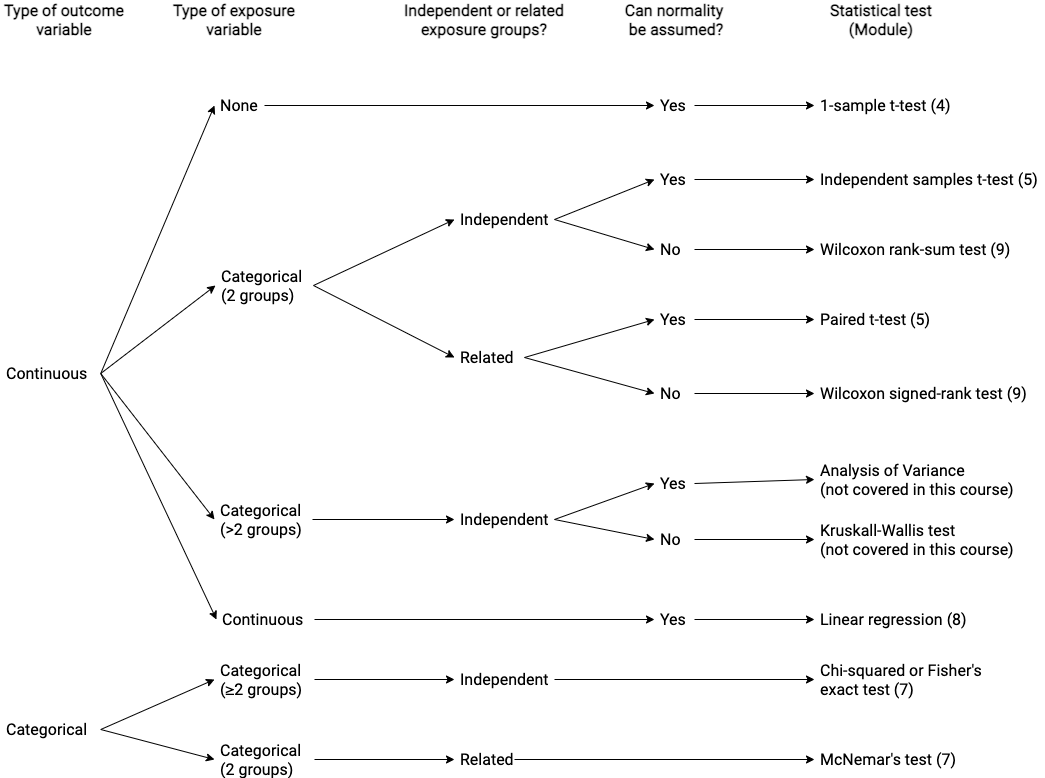
\includegraphics[width=1\linewidth,height=\textheight,keepaspectratio]{img/misc/analysis-flowchart.png}

\bookmarksetup{startatroot}

\chapter*{References}\label{references}
\addcontentsline{toc}{chapter}{References}

\markboth{References}{References}

\protect\phantomsection\label{refs}
\begin{CSLReferences}{1}{1}
\bibitem[\citeproctext]{ref-armitage_etal13}
Armitage, Peter, Geoffrey Berry, and J. N. S. Matthews. 2013.
\emph{Statistical {Methods} in {Medical Research}}. 4th ed.
Wiley-Blackwell.

\bibitem[\citeproctext]{ref-australianbureauofstatistics24}
Australian Bureau of Statistics. 2024. \emph{Causes of {Death},
{Australia}, 2023}.
Https://www.abs.gov.au/statistics/health/causes-death/causes-death-australia/latest-release.

\bibitem[\citeproctext]{ref-australianinstituteofhealthandwelfare24}
Australian Institute of Health and Welfare. 2024. {``Australia's Mothers
and Babies.''} In \emph{Australian Institute of Health and Welfare}.
Https://www.aihw.gov.au/reports/mothers-babies/australias-mothers-babies/contents/about.

\bibitem[\citeproctext]{ref-australianinstituteofhealthandwelfare25}
Australian Institute of Health and Welfare. 2025. \emph{Australia's
Health}. Https://www.aihw.gov.au/reports-data/australias-health.

\bibitem[\citeproctext]{ref-bland15}
Bland, Martin. 2015. \emph{An {Introduction} to {Medical Statistics}}.
4th Edition. Oxford University Press.

\bibitem[\citeproctext]{ref-boers18}
Boers, Maarten. 2018. {``Graphics and Statistics for Cardiology:
Designing Effective Tables for Presentation and Publication.''}
\emph{Heart} 104 (3): 192--200.
\url{https://doi.org/10.1136/heartjnl-2017-311581}.

\bibitem[\citeproctext]{ref-brown_etal01}
Brown, Lawrence D., T. Tony Cai, and Anirban DasGupta. 2001. {``Interval
{Estimation} for a {Binomial Proportion}.''} \emph{Statistical Science}
16 (2): 101--17. \url{https://www.jstor.org/stable/2676784}.

\bibitem[\citeproctext]{ref-deeks98}
Deeks, Jon. 1998. {``When Can Odds Ratios Mislead?''} \emph{BMJ} 317
(7166): 1155. \url{https://doi.org/10.1136/bmj.317.7166.1155a}.

\bibitem[\citeproctext]{ref-delacre_etal17}
Delacre, Marie, Daniël Lakens, and Christophe Leys. 2017. \emph{Why
{Psychologists Should} by {Default Use Welch}'s t-Test {Instead} of
{Student}'s t-Test}. 30 (1): 92. \url{https://doi.org/10.5334/irsp.82}.

\bibitem[\citeproctext]{ref-freiman_etal78}
Freiman, Jennie A., Thomas C. Chalmers, Harry Smith, and Roy R. Kuebler.
1978. {``The {Importance} of {Beta}, the {Type II Error} and {Sample
Size} in the {Design} and {Interpretation} of the {Randomized Control
Trial}.''} \emph{New England Journal of Medicine} 299 (13): 690--94.
\url{https://doi.org/10.1056/NEJM197809282991304}.

\bibitem[\citeproctext]{ref-kirkwood_sterne01}
Kirkwood, Betty, and Jonathan Sterne. 2001. \emph{Essentials of {Medical
Statistics}}. 2nd edition. Wiley-Blackwell.

\bibitem[\citeproctext]{ref-lowitjainstitute21}
Lowitja Institute. 2021. \emph{Indigenous {Data Governance} and
{Sovereignty}}.
Https://www.lowitja.org.au/wp-content/uploads/2023/10/328550\_data-governance-and-sovereignty.pdf.

\bibitem[\citeproctext]{ref-nationalindigenousaustraliansagency24}
National Indigenous Australians Agency. 2024. {``Framework for
{Governance} of {Indigenous Data} \textbar{} {NIAA}.''} In
\emph{Framework for Governance of Indigenous Data}.
Https://www.niaa.gov.au/resource-centre/framework-governance-indigenous-data.

\bibitem[\citeproctext]{ref-ruxton06}
Ruxton, Graeme D. 2006. {``The Unequal Variance t-Test Is an Underused
Alternative to {Student}'s t-Test and the {Mann}--{Whitney U} Test.''}
\emph{Behavioral Ecology} 17 (4): 688--90.
\url{https://doi.org/10.1093/beheco/ark016}.

\bibitem[\citeproctext]{ref-schmidt_kohlmann08}
Schmidt, Carsten Oliver, and Thomas Kohlmann. 2008. {``When to Use the
Odds Ratio or the Relative Risk?''} \emph{International Journal of
Public Health} 53 (3): 165--67.
\url{https://doi.org/10.1007/s00038-008-7068-3}.

\bibitem[\citeproctext]{ref-schober_etal18}
Schober, Patrick, Christa Boer, and Lothar A. Schwarte. 2018.
{``Correlation {Coefficients}: {Appropriate Use} and
{Interpretation}.''} \emph{Anesthesia \& Analgesia} 126 (5): 1763.
\url{https://doi.org/10.1213/ANE.0000000000002864}.

\bibitem[\citeproctext]{ref-therneau_grambsch10}
Therneau, Terry M., and Patricia M. Grambsch. 2010. \emph{Modeling
{Survival Data}: {Extending} the {Cox Model}}. Springer.

\bibitem[\citeproctext]{ref-universityofcaliforniairvine}
University of California Irvine. n.d. \emph{{UCI Machine Learning
Repository}}. Https://archive.ics.uci.edu/.

\bibitem[\citeproctext]{ref-vickers_etal20}
Vickers, Andrew J., Melissa J. Assel, Daniel D. Sjoberg, et al. 2020.
{``Guidelines for {Reporting} of {Figures} and {Tables} for {Clinical
Research} in {Urology}.''} \emph{European Urology}, ahead of print, May.
\url{https://doi.org/10.1016/j.eururo.2020.04.048}.

\bibitem[\citeproctext]{ref-walter_etal21}
Walter, Maggie, Raymond Lovett, Bobby Maher, et al. 2021. {``Indigenous
{Data Sovereignty} in the {Era} of {Big Data} and {Open Data}.''}
\emph{Australian Journal of Social Issues} 56 (2): 143--56.
\url{https://doi.org/10.1002/ajs4.141}.

\bibitem[\citeproctext]{ref-webb_etal16}
Webb, Penny, Chris Bain, and Andrew Page. 2016. \emph{Essential
{Epidemiology}: {An Introduction} for {Students} and {Health
Professionals}}. 3rd edition. Cambridge University Press.

\bibitem[\citeproctext]{ref-west21}
West, Robert M. 2021. {``Best Practice in Statistics: {Use} the {Welch}
t-Test When Testing the Difference Between Two Groups.''} \emph{Annals
of Clinical Biochemistry} 58 (4): 267--69.
\url{https://doi.org/10.1177/0004563221992088}.

\bibitem[\citeproctext]{ref-woodward13}
Woodward, Mark. 2013. \emph{Epidemiology: {Study Design} and {Data
Analysis}}. 3rd edition. {Chapman and Hall/CRC}.

\end{CSLReferences}


\backmatter


\end{document}
